\documentclass[twoside]{book}

% Packages required by doxygen
\usepackage{fixltx2e}
\usepackage{calc}
\usepackage{doxygen}
\usepackage[export]{adjustbox} % also loads graphicx
\usepackage{graphicx}
\usepackage[utf8]{inputenc}
\usepackage{makeidx}
\usepackage{multicol}
\usepackage{multirow}
\PassOptionsToPackage{warn}{textcomp}
\usepackage{textcomp}
\usepackage[nointegrals]{wasysym}
\usepackage[table]{xcolor}

% Font selection
\usepackage[T1]{fontenc}
\usepackage[scaled=.90]{helvet}
\usepackage{courier}
\usepackage{amssymb}
\usepackage{sectsty}
\renewcommand{\familydefault}{\sfdefault}
\allsectionsfont{%
  \fontseries{bc}\selectfont%
  \color{darkgray}%
}
\renewcommand{\DoxyLabelFont}{%
  \fontseries{bc}\selectfont%
  \color{darkgray}%
}
\newcommand{\+}{\discretionary{\mbox{\scriptsize$\hookleftarrow$}}{}{}}

% Page & text layout
\usepackage{geometry}
\geometry{%
  a4paper,%
  top=2.5cm,%
  bottom=2.5cm,%
  left=2.5cm,%
  right=2.5cm%
}
\tolerance=750
\hfuzz=15pt
\hbadness=750
\setlength{\emergencystretch}{15pt}
\setlength{\parindent}{0cm}
\setlength{\parskip}{3ex plus 2ex minus 2ex}
\makeatletter
\renewcommand{\paragraph}{%
  \@startsection{paragraph}{4}{0ex}{-1.0ex}{1.0ex}{%
    \normalfont\normalsize\bfseries\SS@parafont%
  }%
}
\renewcommand{\subparagraph}{%
  \@startsection{subparagraph}{5}{0ex}{-1.0ex}{1.0ex}{%
    \normalfont\normalsize\bfseries\SS@subparafont%
  }%
}
\makeatother

% Headers & footers
\usepackage{fancyhdr}
\pagestyle{fancyplain}
\fancyhead[LE]{\fancyplain{}{\bfseries\thepage}}
\fancyhead[CE]{\fancyplain{}{}}
\fancyhead[RE]{\fancyplain{}{\bfseries\leftmark}}
\fancyhead[LO]{\fancyplain{}{\bfseries\rightmark}}
\fancyhead[CO]{\fancyplain{}{}}
\fancyhead[RO]{\fancyplain{}{\bfseries\thepage}}
\fancyfoot[LE]{\fancyplain{}{}}
\fancyfoot[CE]{\fancyplain{}{}}
\fancyfoot[RE]{\fancyplain{}{\bfseries\scriptsize Generated by Doxygen }}
\fancyfoot[LO]{\fancyplain{}{\bfseries\scriptsize Generated by Doxygen }}
\fancyfoot[CO]{\fancyplain{}{}}
\fancyfoot[RO]{\fancyplain{}{}}
\renewcommand{\footrulewidth}{0.4pt}
\renewcommand{\chaptermark}[1]{%
  \markboth{#1}{}%
}
\renewcommand{\sectionmark}[1]{%
  \markright{\thesection\ #1}%
}

% Indices & bibliography
\usepackage{natbib}
\usepackage[titles]{tocloft}
\setcounter{tocdepth}{3}
\setcounter{secnumdepth}{5}
\makeindex

% Hyperlinks (required, but should be loaded last)
\usepackage{ifpdf}
\ifpdf
  \usepackage[pdftex,pagebackref=true]{hyperref}
\else
  \usepackage[ps2pdf,pagebackref=true]{hyperref}
\fi
\hypersetup{%
  colorlinks=true,%
  linkcolor=blue,%
  citecolor=blue,%
  unicode%
}

% Custom commands
\newcommand{\clearemptydoublepage}{%
  \newpage{\pagestyle{empty}\cleardoublepage}%
}

\usepackage{caption}
\captionsetup{labelsep=space,justification=centering,font={bf},singlelinecheck=off,skip=4pt,position=top}

%===== C O N T E N T S =====

\begin{document}

% Titlepage & ToC
\hypersetup{pageanchor=false,
             bookmarksnumbered=true,
             pdfencoding=unicode
            }
\pagenumbering{alph}
\begin{titlepage}
\vspace*{7cm}
\begin{center}%
{\Large W\+R\+E\+N\+CH \\[1ex]\large 1.\+4 }\\
\vspace*{1cm}
{\large Generated by Doxygen 1.8.13}\\
\end{center}
\end{titlepage}
\clearemptydoublepage
\pagenumbering{roman}
\tableofcontents
\clearemptydoublepage
\pagenumbering{arabic}
\hypersetup{pageanchor=true}

%--- Begin generated contents ---
\chapter{Overview}
\label{index}\hypertarget{index}{}User DocumentationOther\+: \href{../developer/}{\tt Developer} -\/ \href{../internal/}{\tt Internal}

 ~\newline
~\newline


\href{http://wrench-project.org}{\tt W\+R\+E\+N\+CH} enables novel avenues for scientific workflow use, research, development, and education. W\+R\+E\+N\+CH capitalizes on recent and critical advances in the state of the art of distributed platform/application simulation. W\+R\+E\+N\+CH builds on top of the open-\/source \href{http://simgrid.gforge.inria.fr}{\tt Sim\+Grid} simulation framework. Sim\+Grid enables the simulation of large-\/scale distributed applications in a way that is accurate (via validated simulation models), scalable (low ratio of simulation time to simulated time, ability to run large simulations on a single computer with low compute, memory, and energy footprints), and expressive (ability to simulate arbitrary platform, application, and execution scenarios). W\+R\+E\+N\+CH provides directly usable high-\/level simulation abstractions using Sim\+Grid as a foundation.

In a nutshell, W\+R\+E\+N\+CH makes it possible to\+:


\begin{DoxyItemize}
\item Prototype implementations of Workflow Management System (W\+MS) components and underlying algorithms;
\item Quickly, scalably, and accurately simulate arbitrary workflow and platform scenarios for a simulated W\+MS implementation; and
\item Run extensive experimental campaigns to conclusively compare workflow executions, platform architectures, and W\+MS algorithms and designs.
\end{DoxyItemize}

~\newline
\hypertarget{index_overview-architecture}{}\section{Architecture}\label{index_overview-architecture}
W\+R\+E\+N\+CH is an {\itshape open-\/source library} for developing simulators. It is neither a graphical interface nor a stand-\/alone simulator. W\+R\+E\+N\+CH exposes several high-\/level simulation abstractions to provide high-\/level {\bfseries building blocks} for developing custom simulators.

W\+R\+E\+N\+CH comprises four distinct layers\+:


\begin{DoxyItemize}
\item {\bfseries Simulation Core\+:} All necessary simulation models and base abstractions (computing, communicating, storing), provided by \href{http://simgrid.gforge.inria.fr}{\tt Sim\+Grid}.
\item {\bfseries Simulated Core CI Services\+:} abstractions for simulated cyberinfrastructure (CI) components that can be used by a W\+MS to execute workflows (compute services, storage services, network proximity services, data location services, etc.).
\item {\bfseries Simulated W\+MS\+:} simulated W\+MS implementations (e.\+g., simulated existing production W\+M\+Ss, simulated W\+MS research prototypes).
\item {\bfseries Top-\/\+Level Simulation\+:} a top-\/level set of abstractions to instantiate and simulate the execution of arbitrary workflows on arbitrary platforms using a particular W\+MS implementation.
\end{DoxyItemize}

\hypertarget{index_overview-users}{}\section{Three Classes of Users}\label{index_overview-users}
W\+R\+E\+N\+CH is intended for three different classes of users\+:


\begin{DoxyItemize}
\item {\bfseries W\+MS Users} use W\+R\+E\+N\+CH to simulate workflow executions using already implemented W\+MS implementations and Core services.
\item {\bfseries W\+MS Developers/\+Researchers} use W\+R\+E\+N\+CH to prototype and evaluate software W\+MS designs and/or to investigate and evaluate novel algorithms to be implemented in W\+M\+Ss, or experimented in novel CI (interacting with already implemented Core Services).
\item {\bfseries Internal Developers} contribute to the W\+R\+E\+N\+CH code, and in particular, implement new Core Services.
\end{DoxyItemize}\hypertarget{index_overview-users-levels}{}\subsection{Three Levels of A\+P\+I Documentation}\label{index_overview-users-levels}
The W\+R\+E\+N\+CH library provides three {\itshape incremental} levels of documentation, each targeting an A\+PI level\+:

{\bfseries User\+:} targets users who want to use W\+R\+E\+N\+CH for simulating the execution of scientific workflows in different simulation scenarios, using existing simulated W\+M\+Ss already implemented using W\+R\+E\+N\+CH. {\itshape Users} are N\+OT expected to develop new simulation abstractions or algorithms. Instead, they only use available simulation components as high-\/level building blocks to quickly build simulators. These simulators can be as simple as a single 50-\/line main() function.

{\bfseries Developer\+:} targets {\itshape W\+MS developers} and {\itshape W\+MS researchers} who work on developing novel W\+MS designs and algorithms. In addition to documentation for all simulation components provided at the {\itshape User} level, {\itshape Developer} documentation include detailed documentation for interacting with simulated Core Services. (\href{../developer/index.html}{\tt See Developer Documentation})

{\bfseries Internal\+:} targets those users who want to contribute code to W\+R\+E\+N\+CH. The {\itshape internal} documentation provides, in addition to both levels above, detailed documentation for all W\+R\+E\+N\+CH classes including binders to Sim\+Grid. This is the A\+PI needed to, for instance, implement new Core Services. (\href{../internal/index.html}{\tt See Internal Documentation})\hypertarget{index_overview-contact}{}\section{Get in Touch}\label{index_overview-contact}
The main channel to reach the W\+R\+E\+N\+CH team is via the support email\+: \href{mailto:support@wrench-project.org?subject=WRENCH Support Contact: Your Topic}{\tt support@wrench-\/project.\+org}.

{\bfseries Bug Report / Feature Request\+:} our preferred channel to report a bug or request a feature is via W\+R\+E\+N\+CH\textquotesingle{}s \href{https://github.com/wrench-project/wrench/issues}{\tt Github Issues Track}. 
\chapter{Installing W\+R\+E\+N\+CH}
\label{install}
\Hypertarget{install}
User DocumentationOther\+: \href{../developer/install.html}{\tt Developer} -\/ \href{../internal/install.html}{\tt Internal}\hypertarget{install_install-prerequisites}{}\section{Prerequisites}\label{install_install-prerequisites}
W\+R\+E\+N\+CH is developed in {\ttfamily C++}. The code follows the C++11 standard, and thus older compilers may fail to compile it. Therefore, we strongly recommend users to satisfy the following requirements\+:


\begin{DoxyItemize}
\item {\bfseries C\+Make} -\/ version 3.\+2.\+3 or higher
\end{DoxyItemize}

And, one of the following\+:
\begin{DoxyItemize}
\item {\bfseries g++} -\/ version 5.\+0 or higher
\item {\bfseries clang} -\/ version 3.\+6 or higher
\end{DoxyItemize}\hypertarget{install_install-prerequisites-dependencies}{}\subsection{Required Dependencies}\label{install_install-prerequisites-dependencies}

\begin{DoxyItemize}
\item \href{https://simgrid.org/}{\tt Sim\+Grid} -- version 3.\+21
\item \href{http://lemon.cs.elte.hu/}{\tt Lemon C++ library} -- version 1.\+3.\+1 or higher
\item \href{http://pugixml.org/}{\tt Pugi\+X\+ML} -- version 1.\+8 or higher
\item \href{https://github.com/nlohmann/json}{\tt J\+S\+ON for Modern C++} -- version 2.\+1.\+1 or higher
\end{DoxyItemize}\hypertarget{install_install-prerequisites-opt-dependencies}{}\subsection{Optional Dependencies}\label{install_install-prerequisites-opt-dependencies}

\begin{DoxyItemize}
\item \href{https://github.com/google/googletest}{\tt Google Test} -- version 1.\+8 or higher (only required for running test cases)
\item \href{http://www.doxygen.org}{\tt Doxygen} -- version 1.\+8 or higher (only required for generating documentation)
\item \href{https://gitlab.inria.fr/batsim/batsched}{\tt Batsched} -- only needed for realistic simulation of resource managed by production batch schedulers
\end{DoxyItemize}\hypertarget{install_install-source}{}\section{Source Install}\label{install_install-source}
\hypertarget{install_install-source-build}{}\subsection{Building W\+R\+E\+N\+CH}\label{install_install-source-build}
You can download the {\itshape wrench-\/1.\+4.\+tar.\+gz} archive from the \href{https://github.com/wrench-project/wrench/releases}{\tt Git\+Hub releases} page and install it as follows\+:


\begin{DoxyCode}
tar xf wrench-1.4.tar.gz
cd wrench-1.4
cmake .
make
make install # try "sudo make install" if you do not have write privileges
\end{DoxyCode}


To enable the use of Batsched (provided you have installed that package, see above)\+: 
\begin{DoxyCode}
cmake -DENABLE\_BATSCHED=on .
\end{DoxyCode}


If you want to stay on the bleeding edge, you should get the latest git version, and recompile it as you would do for an official archive\+:


\begin{DoxyCode}
git clone https://github.com/wrench-project/wrench
\end{DoxyCode}
\hypertarget{install_install-source-targets}{}\subsection{Existing Compilation Targets}\label{install_install-source-targets}
In most cases, compiling and installing W\+R\+E\+N\+CH is enough\+:


\begin{DoxyCode}
make
make install # try "sudo make install" if you do not have write privileges
\end{DoxyCode}


In addition, several compilation targets are provided in W\+R\+E\+N\+CH\+:


\begin{DoxyCode}
make doc               # Builds WRENCH documentation (in the ./docs directory) - Requires Doxygen
make unit\_tests        # Builds WRENCH unit tests  (run them by typing ./unit\_tests) - Requires Google Test
\end{DoxyCode}


If you want to see actual compiler and linker invocations, add V\+E\+R\+B\+O\+SE=1 to your compilation command\+:


\begin{DoxyCode}
make VERBOSE=1
\end{DoxyCode}
\hypertarget{install_install-docker}{}\section{Docker Containers}\label{install_install-docker}
W\+R\+E\+N\+CH is also distributed in Docker containers. Please, visit the \href{https://hub.docker.com/r/wrenchproject/wrench/}{\tt W\+R\+E\+N\+CH\textquotesingle{}s Repository on Docker Hub} to pull W\+R\+E\+N\+CH\textquotesingle{}s Docker images.

The {\ttfamily latest} tag provides a container with the latest \href{https://github.com/wrench-project/wrench/releases}{\tt W\+R\+E\+N\+CH\textquotesingle{}s release}\+:


\begin{DoxyCode}
docker pull wrenchproject/wrench 
# or
docker run -it wrenchproject/wrench /bin/bash
\end{DoxyCode}


The {\ttfamily unstable} tag provides a container with the current code in the Git\+Hub\textquotesingle{}s {\ttfamily master} branch\+:


\begin{DoxyCode}
docker pull wrenchproject/wrench:unstable
# or
docker run -it wrenchproject/wrench:unstable /bin/bash
\end{DoxyCode}


Additional tags are available for all W\+R\+E\+N\+CH releases.\hypertarget{install_install-troubleshooting}{}\subsection{Installation Troubleshooting}\label{install_install-troubleshooting}
\subparagraph*{{\ttfamily Could N\+OT find Pkg\+Config (missing\+: P\+K\+G\+\_\+\+C\+O\+N\+F\+I\+G\+\_\+\+E\+X\+E\+C\+U\+T\+A\+B\+LE)}}


\begin{DoxyItemize}
\item This error on Mac\+OS is because the {\ttfamily pkg-\/config} package is not installed
\item Solution\+: install this package
\begin{DoxyItemize}
\item Mac\+Ports\+: {\ttfamily sudo port install pkg-\/config}
\item Brew\+: {\ttfamily sudo brew install pkg-\/config} 
\end{DoxyItemize}
\end{DoxyItemize}
\chapter{Getting Started}
\label{getting-started}
\Hypertarget{getting-started}
User DocumentationOther\+: \href{../developer/getting-started.html}{\tt Developer} -\/ \href{../internal/getting-started.html}{\tt Internal}

The first step is to install the W\+R\+E\+N\+CH library, following the instructions on the \hyperlink{install}{installation page}.\hypertarget{getting-started_getting-started-example}{}\section{Running a First Example}\label{getting-started_getting-started-example}
Typing {\ttfamily make} in the top-\/level directory will compile the examples, and {\ttfamily make install} will put the examples binaries in the {\ttfamily /usr/local/bin} folder (for Mac\+OS and most Linux distributions).

W\+R\+E\+N\+CH provides a simple example in the {\ttfamily examples/simple-\/example} directory, which generates two executables\+: a cloud-\/based example {\ttfamily wrench-\/simple-\/example-\/cloud}, and a batch-\/system-\/based (e.\+g., S\+L\+U\+RM) example {\ttfamily wrench-\/simple-\/example-\/batch}. To run the examples, simply use one of the following commands\+:


\begin{DoxyCode}
# Runs the cloud-based implementation
wrench-simple-example-cloud \(\backslash\)
    <PATH-TO-WRENCH-FOLDER>/examples/simple-example/platform\_files/cloud\_hosts.xml \(\backslash\)
    <PATH-TO-WRENCH-FOLDER>/examples/simple-example/workflow\_files/genome.dax

# Runs the batch-based implementation
wrench-simple-example-batch \(\backslash\)
    <PATH-TO-WRENCH-FOLDER>/examples/simple-example/platform\_files/batch\_hosts.xml \(\backslash\)
    <PATH-TO-WRENCH-FOLDER>/examples/simple-example/workflow\_files/genome.dax
\end{DoxyCode}
\hypertarget{getting-started_getting-started-example-simple}{}\subsection{Understanding the Simple Example}\label{getting-started_getting-started-example-simple}
Both versions of the example (cloud of batch) require two command-\/line arguments\+: (1) a \href{http://simgrid.gforge.inria.fr/simgrid/3.19/doc/platform.html}{\tt Sim\+Grid virtual platform description file}; and (2) a W\+R\+E\+N\+CH workflow file.


\begin{DoxyItemize}
\item {\bfseries Sim\+Grid simulated platform description file\+:} A \href{http://simgrid.gforge.inria.fr}{\tt Sim\+Grid} simulation must be provided with the description of the platform on which an application execution is to be simulated. This is done via a platform description file, in X\+ML, that includes definitions of compute hosts, clusters of hosts, storage resources, network links, routes between hosts, etc. A detailed description on how to create a platform description file can be found \href{http://simgrid.gforge.inria.fr/simgrid/3.19/doc/platform.html}{\tt here}.
\item {\bfseries W\+R\+E\+N\+CH workflow file\+:} W\+R\+E\+N\+CH provides native parsers for \href{http://workflowarchive.org}{\tt D\+AX} (D\+AG in X\+ML) and \href{https://github.com/wrench-project/wrench/tree/master/doc/schemas}{\tt J\+S\+ON} workflow description file formats. Refer to their respective Web sites for detailed documentation.
\end{DoxyItemize}

The source file for the cloud-\/based simulator is at {\ttfamily examples/simple-\/example/\+Simulator\+Cloud.\+cpp} and at {\ttfamily examples/simple-\/example/\+Simulator\+Batch.\+cpp} for the batch-\/based example. These source files, which are heavily commented, and perform the following\+:


\begin{DoxyItemize}
\item The first step is to read and parse the workflow and the platform files, and to create a simulation object ({\ttfamily \hyperlink{classwrench_1_1_simulation}{wrench\+::\+Simulation}}).
\item A storage service ({\ttfamily \hyperlink{classwrench_1_1_simple_storage_service}{wrench\+::\+Simple\+Storage\+Service}}) is created and deployed on a host.
\item A cloud ({\ttfamily \hyperlink{classwrench_1_1_cloud_service}{wrench\+::\+Cloud\+Service}}) or a batch ({\ttfamily \hyperlink{classwrench_1_1_batch_service}{wrench\+::\+Batch\+Service}}) service is created and deployed on a host. Both services are seen by the simulation as compute services ({\ttfamily \hyperlink{classwrench_1_1_compute_service}{wrench\+::\+Compute\+Service}}) – jobs can then be submitted to these services.
\item A Workflow Management System ({\ttfamily \hyperlink{classwrench_1_1_w_m_s}{wrench\+::\+W\+MS}}) is instantiated (in this case the {\ttfamily Simple\+W\+MS}) with a reference to a workflow object ({\ttfamily \hyperlink{classwrench_1_1_workflow}{wrench\+::\+Workflow}}) and a scheduler ({\ttfamily wrench\+::\+Scheduler}). The scheduler implements the decision-\/making algorithms inside the W\+MS. These algorithms are modularized (so that the same W\+MS implementation can be iniated with various decision-\/making algorithms in different simulations). The source codes for the schedulers, which is of interest to \char`\"{}\+Developers\char`\"{} (i.\+e., those users who use the W\+R\+E\+N\+CH Developer A\+PI), is in directory {\ttfamily examples/scheduler}.
\item A file registry ({\ttfamily \hyperlink{classwrench_1_1_file_registry_service}{wrench\+::\+File\+Registry\+Service}}), a.\+k.\+a. a file replica catalog, which keeps track of files stored in different storage services, is deployed on a host.
\item Workflow input files are staged on the storage service
\item The simulation is launched, executes, and completes.
\item Timestamps can be retrieved to analyze the simulated execution.
\end{DoxyItemize}

This simple example can be used as a blueprint for starting a large W\+R\+E\+N\+C\+H-\/based simulation project. The next section provides further details about this process.\hypertarget{getting-started_getting-started-wrench-init}{}\section{W\+R\+E\+N\+C\+H Initialization Tool}\label{getting-started_getting-started-wrench-init}
The {\ttfamily wrench-\/init} tool is a project generator built with W\+R\+E\+N\+CH, which creates a simple project structure with example class files, as follows\+:


\begin{DoxyCode}
project-folder/
├── CMakeLists.txt
├── README.md
├── src/
│   ├── SimpleSimulator.cpp
│   ├── SimpleStandardJobScheduler.cpp
│   ├── SimpleStandardJobScheduler.h
│   ├── SimpleWMS.cpp
│   └── SimpleWMS.h 
├── test/
├── doc/
├── build/
└── data/
    ├── platform-files/
    └── workflow-files/
\end{DoxyCode}


The {\ttfamily Simple\+Simulator.\+cpp} source file contains the class representing the simulator (either cloud or batch). {\ttfamily Simple\+Standard\+Job\+Scheduler.\+h} and {\ttfamily Simple\+Standard\+Job\+Scheduler.\+cpp} contain a simple implementation for a {\ttfamily \hyperlink{classwrench_1_1_standard_job_scheduler}{wrench\+::\+Standard\+Job\+Scheduler}}; {\ttfamily Simple\+W\+M\+S.\+h} and {\ttfamily Simple\+W\+M\+S.\+cpp} denote the implementation of a simple workflow management system. Example platform and workflow files are also generated into the {\ttfamily data} folder. These files provide the minimum necessary implementation for a W\+R\+E\+N\+C\+H-\/enabled simulator.

The {\ttfamily wrench-\/init} tool only requires a single argument, the name of the folder where the project skeleton will be generated\+:


\begin{DoxyCode}
$ wrench-init <PROJECT\_FOLDER>
\end{DoxyCode}


Additional options supported by the tool can be found by using the {\ttfamily wrench-\/init -\/-\/help} command.\hypertarget{getting-started_getting-started-prep}{}\section{Preparing the Environment}\label{getting-started_getting-started-prep}
\hypertarget{getting-started_getting-started-prep-import}{}\subsection{Importing W\+R\+E\+N\+CH}\label{getting-started_getting-started-prep-import}
For ease of use, all W\+R\+E\+N\+CH abstractions are accessed via a single include statement\+:


\begin{DoxyCode}
\textcolor{preprocessor}{#include <wrench.h>}
\end{DoxyCode}
\hypertarget{getting-started_getting-started-prep-cmakelists}{}\subsection{Creating Your C\+Make\+Lists.\+txt File}\label{getting-started_getting-started-prep-cmakelists}
Below is an example of a {\ttfamily C\+Make\+Lists.\+txt} file that can be used as a starting template for developing a W\+R\+E\+N\+CH application compiled using cmake\+:


\begin{DoxyCode}
cmake\_minimum\_required(VERSION 3.2)
message(STATUS "Cmake version $\{CMAKE\_MAJOR\_VERSION\}.$\{CMAKE\_MINOR\_VERSION\}.$\{CMAKE\_PATCH\_VERSION\}")

project(YOUR\_PROJECT\_NAME)

add\_definitions("-Wall -Wno-unused-variable -Wno-unused-private-field")

set(CMAKE\_CXX\_STANDARD 11)

# include directories for dependencies and WRENCH libraries
include\_directories(src/ /usr/local/include /usr/local/include/wrench)

# source files
set(SOURCE\_FILES
        src/main.cpp
        )

# test files
set(TEST\_FILES
        )

# wrench library and dependencies
find\_library(WRENCH\_LIBRARY NAMES wrench)
find\_library(SIMGRID\_LIBRARY NAMES simgrid)
find\_library(PUGIXML\_LIBRARY NAMES pugixml)
find\_library(LEMON\_LIBRARY NAMES emon)
find\_library(GTEST\_LIBRARY NAMES gtest)

# generating the executable
add\_executable(my-executable $\{SOURCE\_FILES\})
target\_link\_libraries(my-executable 
                        $\{WRENCH\_LIBRARY\} 
                        $\{SIMGRID\_LIBRARY\} 
                        $\{PUGIXML\_LIBRARY\} 
                        $\{LEMON\_LIBRARY\}
                     )

install(TARGETS my-executable DESTINATION bin)

# generating unit tests
add\_executable(unit\_tests EXCLUDE\_FROM\_ALL 
                 $\{SOURCE\_FILES\} 
                 $\{TEST\_FILES\}
              )
target\_link\_libraries(unit\_tests 
                        $\{GTEST\_LIBRARY\} wrench -lpthread -lm
                     )
\end{DoxyCode}
 
\chapter{W\+R\+E\+N\+CH 101}
\label{wrench-101}
\Hypertarget{wrench-101}
User DocumentationOther\+: \href{../developer/wrench-101.html}{\tt Developer} -\/ \href{../internal/wrench-101.html}{\tt Internal}

W\+R\+E\+N\+CH 101 is a page and a set of documents that provide detailed information for each W\+R\+E\+N\+CH\textquotesingle{}s \hyperlink{index_overview-users}{classes of users}, and higher-\/level content than the \href{./annotated.html}{\tt A\+PI Reference}. For instructions on how to \hyperlink{install}{install}, run a \hyperlink{getting-started}{first example}, or \hyperlink{getting-started_getting-started-prep}{create a basic W\+R\+E\+N\+C\+H-\/based simulator}, please refer to their respective sections in the documentation.

This {\bfseries User 101} guide describes all the W\+R\+E\+N\+CH simulation components (building blocks) necessary to build a custom simulator and run simulation scenarios.



\hypertarget{wrench-101_wrench-101-simulator-10000ft}{}\section{10,000-\/ft view of a W\+R\+E\+N\+C\+H-\/based simulator}\label{wrench-101_wrench-101-simulator-10000ft}
A W\+R\+E\+N\+C\+H-\/based simulator can be as simple as a single {\ttfamily main()} function that first creates a platform to be simulated (the hardware) and a set of services that run on the platform (the software). These services correspond to software that knows how to store data, perform computation, and many other useful things that real-\/world cyberinfrastructure services can do.

The simulator then needs to create a workflow (or a set of workflows) to be executed, which consists of a set of compute tasks each with input and output files, and thus data-\/dependencies. A special service is then created, called a Workflow Management System (W\+MS), that will be in charge of executing the workflow on the platform. (This service must have been implemented by a W\+R\+E\+N\+CH \char`\"{}developer\char`\"{}, i.\+e., a user that has used the Developer A\+PI). The set of input files to the workflow, if any, are staged on the platform at particular storage locations.

The simulation is then launched via a single call. When this call returns, the W\+MS has cleanly\+\_\+terminated (typically after completing the execution of the workflow, or failing to executed it) and the simulation output can be analyzed.\hypertarget{wrench-101_wrench-101-simulator-blueprint}{}\section{Blueprint for a W\+R\+E\+N\+C\+H-\/based simulator}\label{wrench-101_wrench-101-simulator-blueprint}
Here are the steps that a W\+R\+E\+N\+C\+H-\/based simulator typically follows\+:


\begin{DoxyEnumerate}
\item {\bfseries Create and initialize a simulation} -- In W\+R\+E\+N\+CH, a user simulation is defined via the {\ttfamily \hyperlink{classwrench_1_1_simulation}{wrench\+::\+Simulation}} class. An instance of this class must be created, and the {\ttfamily \hyperlink{classwrench_1_1_simulation_a3c6d35f1f77f35cbc727ce31e5689992}{wrench\+::\+Simulation\+::init()}} method is called to initialize the simulation (and parse W\+R\+E\+N\+C\+H-\/specific and \href{http://simgrid.gforge.inria.fr/simgrid/3.19/doc/options.html}{\tt Sim\+Grid-\/specific} command-\/line arguments). Two useful such arguments are {\ttfamily -\/-\/help-\/wrench}, which displays help messages about optional W\+R\+E\+N\+C\+H-\/specific command-\/line arguments, and {\ttfamily -\/-\/help-\/simgrid}, which displays help messages about optional Simgrid-\/specific command-\/line arguments.
\item {\bfseries Instantiate a simulated platform} -- This is done with the {\ttfamily \hyperlink{classwrench_1_1_simulation_ae22639abf6ede9f345b382f5ffe19b0e}{wrench\+::\+Simulation\+::instantiate\+Platform()}} method which takes as argument a \href{http://simgrid.gforge.inria.fr/simgrid/3.17/doc/platform.html}{\tt Sim\+Grid virtual platform description file}. Any \href{http://simgrid.gforge.inria.fr}{\tt Sim\+Grid} simulation must be provided with the description of the platform on which an application/system execution is to be simulated (compute hosts, clusters of hosts, storage resources, network links, routers, routes between hosts, etc.)
\item {\bfseries Instantiate services on the platform} -- The {\ttfamily \hyperlink{classwrench_1_1_simulation_ad1f5c12285ecfaf5a2ce7dab5ec8b4c5}{wrench\+::\+Simulation\+::add()}} method is used to add services to the simulation. Each class of service is created with a particular constructor, which also specifies host(s) on which the service is to be started. Typical kinds of services include compute services, storage services, network proximity services, and file registry services.
\item {\bfseries Create at least one workflow} -- This is done by creating an instance of the {\ttfamily \hyperlink{classwrench_1_1_workflow}{wrench\+::\+Workflow}} class, which has methods to manually add tasks and files to the workflow application, but also methods to import workflows from standard workflow description files (\href{http://workflowarchive.org}{\tt D\+AX} and \href{https://github.com/wrench-project/wrench/tree/master/doc/schemas}{\tt J\+S\+ON}). If there are input files to the workflow\textquotesingle{}s entry tasks, these must be staged on instantiated storage services.
\item {\bfseries Instantiate at least one W\+MS per workflow} -- At least one of the services instantiated must be a {\ttfamily \hyperlink{classwrench_1_1_w_m_s}{wrench\+::\+W\+MS}} instance, i.\+e., a service that is in charge of executing the workflow, as implemented by a W\+R\+E\+N\+CH \char`\"{}developer\char`\"{} using the \href{../developer/wrench-101.html}{\tt Developer} A\+PI. Associating a workflow to a W\+MS is done via the {\ttfamily \hyperlink{classwrench_1_1_w_m_s_afd2a6ae2f4d792046a6a17d5c0dc313f}{wrench\+::\+W\+M\+S\+::add\+Workflow()}} method.
\item {\bfseries Launch the simulation} -- This is done via the {\ttfamily \hyperlink{classwrench_1_1_simulation_ae9589632de9a2311ed1d7f7747478985}{wrench\+::\+Simulation\+::launch()}} call which first sanity checks the simulation setup and then launches all simulated services, until all W\+MS services have exited (after they have completed or failed to complete workflows).
\item {\bfseries Process simulation output} -- The {\ttfamily \hyperlink{classwrench_1_1_simulation_aff0338aa6831c6ac252cf0673fe68f44}{wrench\+::\+Simulation\+::get\+Output()}} method returns an object that is a collection of time-\/stamped traces of simulation events. These traces can be processed/analyzed at will.
\end{DoxyEnumerate}\hypertarget{wrench-101_wrench-101-simulator-services}{}\section{Available services}\label{wrench-101_wrench-101-simulator-services}
To date, these are the (simulated) services that can be instantiated on the simulated platform\+:


\begin{DoxyItemize}
\item {\bfseries Compute Services} (classes that derive {\ttfamily \hyperlink{classwrench_1_1_compute_service}{wrench\+::\+Compute\+Service}})\+: These are services that know how to compute workflow tasks. These include bare-\/metal servers ({\ttfamily \hyperlink{classwrench_1_1_bare_metal_compute_service}{wrench\+::\+Bare\+Metal\+Compute\+Service}}), cloud platforms ({\ttfamily \hyperlink{classwrench_1_1_cloud_service}{wrench\+::\+Cloud\+Service}}), virtualized cluster platforms ({\ttfamily \hyperlink{classwrench_1_1_virtualized_cluster_service}{wrench\+::\+Virtualized\+Cluster\+Service}}), batch-\/scheduled clusters ({\ttfamily \hyperlink{classwrench_1_1_batch_service}{wrench\+::\+Batch\+Service}}). It is not technically required to instantiate a compute service, but then no workflow task can be executed by the W\+MS.
\item {\bfseries Storage Services} (classes that derive {\ttfamily \hyperlink{classwrench_1_1_storage_service}{wrench\+::\+Storage\+Service}})\+: These are services that know how to store workflow files, which can then be accessed in reading/writing by the compute services when executing tasks that read/write files. It is not technically required to instantiate a storage service, but then no workflow task can have an input or an output file.
\item {\bfseries File Registry Services} (the {\ttfamily \hyperlink{classwrench_1_1_file_registry_service}{wrench\+::\+File\+Registry\+Service}} class)\+: These services, often known as {\itshape replica catalogs}, are simply databases of $<$filename, list of locations$>$ key-\/value pairs of the storage services on which a copies of files are available. They are used during workflow execution to decide where input files for tasks can be acquired. It is not required to instantiate a file registry service, unless the workflow\textquotesingle{}s entry tasks have input files (because in this case these files have to be stored at some storage services before the execution can start, and all file registry service are then automatically made aware of where these files are stored). Note that some W\+MS implementations may complain if no file registry service is available.
\item {\bfseries Network Proximity Services} (the class {\ttfamily \hyperlink{classwrench_1_1_network_proximity_service}{wrench\+::\+Network\+Proximity\+Service}})\+: These are services that monitor the network and maintain a database of host-\/to-\/host network distances. This database can be queried by W\+M\+Ss to make informed decisions, e.\+g., to pick from which storage service a file should be retrieved so as to reduce communication time. Typically, network distances are estimated based on round-\/trip-\/times between hosts. It is not required to instantiate a network proximity service, but some W\+MS implementations may complain if none is available.
\item {\bfseries Workflow Management Systems (W\+M\+Ss)} (classes that derive {\ttfamily \hyperlink{classwrench_1_1_w_m_s}{wrench\+::\+W\+MS}})\+: A workflow management system provides the mechanisms for executing workflow applications, include decision-\/making for optimizing various objectives (the most common one is to minimize workflow execution time). By default, W\+R\+E\+N\+CH does not provide a W\+MS implementation as part of its core components, however a simple implementation ({\ttfamily wrench\+::\+Simple\+W\+MS}) is available in the {\ttfamily examples/simple-\/example} folder. Please, refer to the \href{../developer/wrench-101.html}{\tt Developer 101 Guide} section for further information on how to develop a W\+MS. At least {\bfseries one} W\+MS should be provided for running a simulation. Additional W\+M\+Ss implementations may also be found in the \href{http://wrench-project.org}{\tt W\+R\+E\+N\+CH project website}.
\end{DoxyItemize}\hypertarget{wrench-101_wrench-101-customizing-services}{}\section{Customizing Services}\label{wrench-101_wrench-101-customizing-services}
Each service is customizable by passing to its constructor a {\itshape property list}, i.\+e., a key-\/value map where each key is a property and each value is a string. Each service defines a property class. For instance, the {\ttfamily \hyperlink{classwrench_1_1_service}{wrench\+::\+Service}} class has an associated {\ttfamily \hyperlink{classwrench_1_1_service_property}{wrench\+::\+Service\+Property}} class, the {\ttfamily \hyperlink{classwrench_1_1_compute_service}{wrench\+::\+Compute\+Service}} class has an associated {\ttfamily \hyperlink{classwrench_1_1_compute_service_property}{wrench\+::\+Compute\+Service\+Property}} class, and so on at all levels of the service class hierarchy.

The A\+PI documentation for these property classes explains what each property means, what possible values are, and what default values are. Other properties have more to do with what the service can or should do when in operation. For instance, the {\ttfamily \hyperlink{classwrench_1_1_batch_service_property}{wrench\+::\+Batch\+Service\+Property}} class defines a {\ttfamily \hyperlink{classwrench_1_1_batch_service_property_aceb0af1c33f5ff2da347f54a484ce32e}{wrench\+::\+Batch\+Service\+Property\+::\+B\+A\+T\+C\+H\+\_\+\+S\+C\+H\+E\+D\+U\+L\+I\+N\+G\+\_\+\+A\+L\+G\+O\+R\+I\+T\+HM}} which specifies what scheduling algorithm a batch service should use for prioritizing jobs. All property classes inherit from the {\ttfamily \hyperlink{classwrench_1_1_service_property}{wrench\+::\+Service\+Property}} class, and one can explore that hierarchy to discover all possible (and there are many) service customization opportunities.

Finally, each service exchanges messages on the network with other services (e.\+g., a W\+MS service sends a \char`\"{}do some work\char`\"{} message to a compute service). The size in bytes, or payload, of all messages can be customized similarly to the properties, i.\+e., by passing a key-\/value map to the service\textquotesingle{}s constructor. For instance, the {\ttfamily \hyperlink{classwrench_1_1_service_message_payload}{wrench\+::\+Service\+Message\+Payload}} class defines a {\ttfamily \hyperlink{classwrench_1_1_service_message_payload_a9efb4a6b2c8876e17a3f636ba5ac17f6}{wrench\+::\+Service\+Message\+Payload\+::\+S\+T\+O\+P\+\_\+\+D\+A\+E\+M\+O\+N\+\_\+\+M\+E\+S\+S\+A\+G\+E\+\_\+\+P\+A\+Y\+L\+O\+AD}} property which can be used to customize the size, in bytes, of the control message sent to the service daemon (that is the entry point to the service) to tell it to terminate. Each service class has a corresponding message payload class, and the A\+PI documentation for these message payload classes details all messages whose payload can be customized.\hypertarget{wrench-101_wrench-101-logging}{}\section{Customizing logging}\label{wrench-101_wrench-101-logging}
When running a W\+R\+E\+N\+CH simulator you will notice that there is quite a bit of logging output. While logging output can be useful to inspect visually the way in which the simulation proceeds, it often becomes necessary to disable it. W\+R\+E\+N\+CH\textquotesingle{}s logging system is a thin layer on top of Sim\+Grid\textquotesingle{}s logging system, and as such is controlled via command-\/line arguments. The simple example in {\ttfamily examples/simple-\/example} is executed as follows, assuming the working directory is {\ttfamily examples/simple-\/example}\+:


\begin{DoxyCode}
./\hyperlink{namespacewrench}{wrench}-simple-example-cloud  platform\_files/cloud\_hosts.xml workflow\_files/genome.dax
\end{DoxyCode}


One first way in which to modify logging is to disable colors, which can be useful to redirect output to a file, is to use the {\ttfamily -\/-\/wrench-\/no-\/color} command-\/line option, anywhere in the argument list, for instance\+:


\begin{DoxyCode}
./\hyperlink{namespacewrench}{wrench}-simple-example-cloud  --\hyperlink{namespacewrench}{wrench}-no-color platform\_files/cloud\_hosts.xml workflow\_files/
      genome.dax
\end{DoxyCode}


Disabling all logging is done with the Sim\+Grid option {\ttfamily -\/-\/wrench-\/no-\/log}\+:


\begin{DoxyCode}
./\hyperlink{namespacewrench}{wrench}-simple-example-cloud  --\hyperlink{namespacewrench}{wrench}-no-log platform\_files/cloud\_hosts.xml workflow\_files/
      genome.dax
\end{DoxyCode}


The above {\ttfamily -\/-\/wrench-\/no-\/log} option is a simple wrapper around the sophisticated Simgrid logging capabilities (it is equivalent to the Simgrid argument {\ttfamily -\/-\/log=root.\+threshold\+:critical}). Details on these capabilities are displayed when passing the {\ttfamily -\/-\/help-\/logs} command-\/line argument to your simulator. In a nutshell particular \char`\"{}log categories\char`\"{} can be toggled on and off. Log category names are attached to {\ttfamily $\ast$.cpp} files in the W\+R\+E\+N\+CH and Sim\+Grid code. Using the {\ttfamily -\/-\/help-\/log-\/categories} command-\/line argument shows the entire log category hierarchy. For instance, there is a log category that is called {\ttfamily wms} for the W\+MS, i.\+e., those logging messages in the {\ttfamily wrench\+:W\+MS} class and a log category that is called {\ttfamily simple\+\_\+wms} for logging message in the {\ttfamily wrench\+::\+Simple\+W\+MS} class, which inherits from {\ttfamily \hyperlink{classwrench_1_1_w_m_s}{wrench\+::\+W\+MS}}. These messages are thus logging output produced by the W\+MS in the simple example. They can be enabled while other messages are disabled as follows\+:


\begin{DoxyCode}
./\hyperlink{namespacewrench}{wrench}-simple-example-cloud   platform\_files/cloud\_hosts.xml workflow\_files/genome.dax --log=root.
      threshold:critical --log=simple\_wms.threshold=debug --log=wms.threshold=debug
\end{DoxyCode}


Use the {\ttfamily -\/-\/help-\/logs} option displays information on the way Sim\+Grid logging works. See the \href{http://simgrid.gforge.inria.fr/simgrid/latest/doc/outcomes_logs.html}{\tt full Sim\+Grid logging documentation} for all details.\hypertarget{wrench-101_wrench-101-simulation-output}{}\section{Analyzing Simulation Output}\label{wrench-101_wrench-101-simulation-output}
Once the {\ttfamily \hyperlink{classwrench_1_1_simulation_ae9589632de9a2311ed1d7f7747478985}{wrench\+::\+Simulation\+::launch()}} method has returned, it is possible to process time-\/stamped traces to analyze simulation output. The {\ttfamily \hyperlink{classwrench_1_1_simulation_aff0338aa6831c6ac252cf0673fe68f44}{wrench\+::\+Simulation\+::get\+Output()}} method returns an instance of {\ttfamily \hyperlink{classwrench_1_1_simulation_output}{wrench\+::\+Simulation\+Output}}. This object has a templated {\ttfamily \hyperlink{classwrench_1_1_simulation_output_a1d03324f34db985d0e181e42cf30cd9d}{wrench\+::\+Simulation\+Output\+::get\+Trace()}} method to retrieve traces for various information types. For instance, the call 
\begin{DoxyCode}
simulation.getOutput().getTrace<wrench::SimulationTimestampTaskCompletion>()
\end{DoxyCode}
 returns a vector of time-\/stamped task completion events. The classes that implement time-\/stamped events are all classes named {\ttfamily wrench\+::\+Simulation\+Timestamp\+Something}, where {\ttfamily Something} is pretty self-\/explanatory (e.\+g., {\ttfamily Task\+Completion}).\hypertarget{wrench-101_wrench-101-energy}{}\section{Measuring Energy Consumption}\label{wrench-101_wrench-101-energy}
W\+R\+E\+N\+CH leverages \href{http://simgrid.gforge.inria.fr/simgrid/latest/doc/group__plugin__energy.html}{\tt Sim\+Grid\textquotesingle{}s energy plugin}, which provides accounting for computing time and dissipated energy in the simulated platform. Sim\+Grid\textquotesingle{}s energy plugin requires host {\bfseries pstate} definitions (levels of performance, C\+PU frequency) in the \href{http://simgrid.gforge.inria.fr/simgrid/latest/doc/platform.html}{\tt X\+ML platform description file}. The following is a list of current available information provided by the plugin\+:


\begin{DoxyItemize}
\item {\ttfamily wrench\+::\+Simulation\+::get\+Energy\+Consumed\+By\+Host()}
\item {\ttfamily wrench\+::\+Simulation\+::get\+Total\+Energy\+Consumed()}
\item {\ttfamily \hyperlink{classwrench_1_1_simulation_adf4675a8c9c62c93bfbd3dc4a4e46556}{wrench\+::\+Simulation\+::set\+Pstate()}}
\item {\ttfamily \hyperlink{classwrench_1_1_simulation_a5e8d5b963d2278c79b49a0ed7db2b933}{wrench\+::\+Simulation\+::get\+Numberof\+Pstates()}}
\item {\ttfamily \hyperlink{classwrench_1_1_simulation_a3d204b229feec1eee4f1e82d92490d81}{wrench\+::\+Simulation\+::get\+Current\+Pstate()}}
\item {\ttfamily \hyperlink{classwrench_1_1_simulation_afdf2ae84f6b3c8b51c5189199bebb52e}{wrench\+::\+Simulation\+::get\+Min\+Power\+Consumption()}}
\item {\ttfamily \hyperlink{classwrench_1_1_simulation_ae76b92ce868c6e6c1683377d869a5b34}{wrench\+::\+Simulation\+::get\+Max\+Power\+Consumption()}}
\item {\ttfamily \hyperlink{classwrench_1_1_simulation_abb75fd040236995186d9ad45434fe069}{wrench\+::\+Simulation\+::get\+List\+Of\+Pstates()}}
\end{DoxyItemize}

{\bfseries Note\+:} The energy plugin is N\+OT enabled by default in W\+R\+E\+N\+CH simulation. To enable the plugin, the {\ttfamily -\/-\/activate-\/energy} command line option should be provided when running a simulator. 
\chapter{Guide}
\label{guide}
\Hypertarget{guide}
User DocumentationOther\+: \href{../developer/guide.html}{\tt Developer} -\/ \href{../internal/guide.html}{\tt Internal}


\begin{DoxyEnumerate}
\item Compute Services
\begin{DoxyEnumerate}
\item \hyperlink{guide-baremetal}{Bare-\/metal Servers}
\item \hyperlink{guide-cloud}{Cloud Platforms}
\item \hyperlink{guide-virtualizedcluster}{Virtualized Cluster Platforms}
\item \hyperlink{guide-batch}{Batch-\/scheduled Clusters}
\item \hyperlink{guide-htcondor}{H\+T\+Condor Workload Management System}
\end{DoxyEnumerate}
\item Storage Services
\begin{DoxyEnumerate}
\item \hyperlink{guide-simplestorage}{Simple}
\end{DoxyEnumerate}
\item File Registry Services
\begin{DoxyEnumerate}
\item \hyperlink{guide-fileregistry}{File Registry Service}
\end{DoxyEnumerate}
\item Network Proximity Services
\begin{DoxyEnumerate}
\item \hyperlink{guide-networkproximity}{Network Proximity Service} 
\end{DoxyEnumerate}
\end{DoxyEnumerate}
\chapter{Bare-\/\+Metal}
\label{guide-baremetal}
\Hypertarget{guide-baremetal}
Internal DocumentationOther\+: \href{../user/guide-baremetal.html}{\tt User} -\/ \href{../developer/guide-baremetal.html}{\tt Developer}\hypertarget{guide-baremetal_guide-baremetal-overview}{}\section{Overview}\label{guide-baremetal_guide-baremetal-overview}
A bare-\/metal is a service that makes it possible to run directly jobs on hardware resources. Think of it as a set of multi-\/core hosts on which multi-\/threaded processes can be started using something like Ssh. The service does not perform any space-\/sharing among the jobs. In other words, jobs submitted to the service execute concurrently in a time-\/shared manner. It is the responsibility of the job submitter to pick hosts and/or numbers of cores for each task, e.\+g., to enforce space-\/sharing of cores. The only resource allocation performed by the service is that it ensures that the R\+AM capacity of a host is not exceeded. Tasks that have non-\/zero R\+AM requirements are queued in F\+C\+FS fashion at each host until there is enough R\+AM to execute them (think of this as each host running an OS that disallows swapping and implements a F\+C\+FS access policy for R\+AM allocation).\hypertarget{guide-baremetal_guide-baremetal-creating}{}\section{Creating a bare-\/metal compute service}\label{guide-baremetal_guide-baremetal-creating}
In W\+R\+E\+N\+CH, a bare-\/metal service represents a compute service ({\ttfamily \hyperlink{classwrench_1_1_compute_service}{wrench\+::\+Compute\+Service}}), which is defined by the {\ttfamily \hyperlink{classwrench_1_1_bare_metal_compute_service}{wrench\+::\+Bare\+Metal\+Compute\+Service}} class. An instantiation of a bare-\/metal service requires the following parameters\+:


\begin{DoxyItemize}
\item The name of a host on which to start the service (this is the entry point to the service);
\item A set of compute hosts in a map ({\ttfamily std\+::map}), where each key is a hostname and each value is a tuple ({\ttfamily std\+::tuple}) with a number of cores and a R\+AM capacity.
\item A scratch space size, i.\+e., the size in bytes of storage local to the bare-\/metal service (used to store workflow files, as needed, during job executions)
\item Maps ({\ttfamily std\+::map}) of configurable properties ({\ttfamily \hyperlink{classwrench_1_1_bare_metal_compute_service_property}{wrench\+::\+Bare\+Metal\+Compute\+Service\+Property}}) and configurable message payloads ({\ttfamily \hyperlink{classwrench_1_1_bare_metal_compute_service_message_payload}{wrench\+::\+Bare\+Metal\+Compute\+Service\+Message\+Payload}}).
\end{DoxyItemize}

The example below shows how to create an instance of a bare-\/metal service that runs on host \char`\"{}\+Gateway\char`\"{}, provides access to 4 cores and 1\+GiB of R\+AM on host \char`\"{}\+Node1\char`\"{} and to 8 cores and 4\+GiB of R\+AM on host \char`\"{}\+Node2\char`\"{}, and has a scratch space of 1\+TiB. Furthermore, the thread startup overhead is configured to be one hundredth of a second\+:


\begin{DoxyCode}
\textcolor{keyword}{auto} baremetal\_cs = simulation->add(
          \textcolor{keyword}{new} \hyperlink{classwrench_1_1_bare_metal_compute_service}{wrench::BareMetalComputeService}(\textcolor{stringliteral}{"Gateway"}, 
                                       \{\{\textcolor{stringliteral}{"Node1"}, std::make\_tuple(4, pow(2,30))\}, \{\textcolor{stringliteral}{"Node2"}, std::make\_tuple
      (8, pow(2,32)\}\},
                                       pow(2,40),
                                       \{\{
      \hyperlink{classwrench_1_1_bare_metal_compute_service_property_a63dfaa7ebb4dc18d236c58384f14dd25}{wrench::BareMetalComputeServiceProperty::THREAD\_STARTUP\_OVERHEAD}
      , \textcolor{stringliteral}{"0.01"}\}\}, 
                                       \{\});
\end{DoxyCode}
\hypertarget{guide-batch_guide-baremetal-creating-properties}{}\subsection{Bare-\/metal service properties}\label{guide-batch_guide-baremetal-creating-properties}
In addition to properties inherited from {\ttfamily \hyperlink{classwrench_1_1_compute_service_property}{wrench\+::\+Compute\+Service\+Property}}, a bare-\/metal service supports the following properties\+:


\begin{DoxyItemize}
\item {\ttfamily \hyperlink{classwrench_1_1_bare_metal_compute_service_property_a63dfaa7ebb4dc18d236c58384f14dd25}{wrench\+::\+Bare\+Metal\+Compute\+Service\+Property\+::\+T\+H\+R\+E\+A\+D\+\_\+\+S\+T\+A\+R\+T\+U\+P\+\_\+\+O\+V\+E\+R\+H\+E\+AD}}
\end{DoxyItemize}\hypertarget{guide-baremetal_guide-baremetal-using}{}\section{Submitting jobs to a bare-\/metal compute service}\label{guide-baremetal_guide-baremetal-using}
As expected, a bare-\/metal service provides implementations of the methods in the {\ttfamily \hyperlink{classwrench_1_1_compute_service}{wrench\+::\+Compute\+Service}} base class. The {\ttfamily \hyperlink{classwrench_1_1_compute_service_abc9e51234c29965341727f07b446ff0c}{wrench\+::\+Compute\+Service\+::submit\+Job()}} method takes as argument service-\/specific arguments as a {\ttfamily std\+::map$<$std\+::string, std\+::string$>$} of key-\/value pairs. The key is a task ID, and the value is the service-\/specific argument for that task. When submitting a job to a bare-\/metal service, arguments can be specified a follows.

For each task, an optional argument can be provided as a string formatted as \char`\"{}hostname\+:num\+\_\+cores\char`\"{}, \char`\"{}hostname\char`\"{}, or \char`\"{}num\+\_\+cores\char`\"{}, where \char`\"{}hostname\char`\"{} is the name of one of the service\textquotesingle{}s compute hosts and \char`\"{}num\+\_\+cores\char`\"{} is an integer (e.\+g., \char`\"{}host1\+:10\char`\"{}, \char`\"{}host1\char`\"{}, \char`\"{}10\char`\"{})\+:


\begin{DoxyItemize}
\item If no value is provided for a task, or if the value is the empty string, then the bare-\/metal service will choose the host on which the task should be executed (typically the host with the lowest current load), and will execute the task with as many cores as possible on that host.
\item If a \char`\"{}hostname\char`\"{} value is provided for a task, then the bare-\/metal service will execute the task on that host, and will execute the task with as many cores as possible on that host.
\item If a \char`\"{}num\+\_\+cores\char`\"{} value is provided for a task, then the bare-\/metal service will choose the host on which the task should be executed (typically the host with the lowest current load), and will execute the task with the specified number of cores.
\item If a \char`\"{}hostname\+:num\+\_\+cores\char`\"{} value is provided for a task, then the bare-\/metal service will execute the task on that host with the specified number of cores.
\end{DoxyItemize}

Here is an example submission to the bare-\/metal service created in the above example, for a 4-\/task job for tasks with I\+Ds \char`\"{}task1\char`\"{}, \char`\"{}task2\char`\"{}, \char`\"{}task3\char`\"{}, and \char`\"{}task4\char`\"{}\+:


\begin{DoxyCode}
\textcolor{comment}{// Create a job manager}
\textcolor{keyword}{auto} job\_manager = this->createJobManager();

\textcolor{comment}{// Create a job}
\textcolor{keyword}{auto} job = job\_manager->createStandardJob(
                 \{this->getWorklow()->getTaskByID(\textcolor{stringliteral}{"task1"}),
                  this->getWorklow()->getTaskByID(\textcolor{stringliteral}{"task2"}),
                  this->getWorklow()->getTaskByID(\textcolor{stringliteral}{"task3"}),
                  this->getWorklow()->getTaskByID(\textcolor{stringliteral}{"task4"})\}, \{\});

\textcolor{comment}{// Create service-specific arguments so that:}
\textcolor{comment}{//   task1 will run on host Node1 with as many cores as possible}
\textcolor{comment}{//   task2 will run on host Node2 with 16 cores}
\textcolor{comment}{//   task3 will run on some host with as many cores as possible}
\textcolor{comment}{//   task4 will run on some host with 4 cores}
std::map<std::string, std::string> service\_specific\_args;
service\_specific\_args[\textcolor{stringliteral}{"task1"}] = \textcolor{stringliteral}{"Node1"};
service\_specific\_args[\textcolor{stringliteral}{"task2"}] = \textcolor{stringliteral}{"Node2:16"};
service\_specific\_args[\textcolor{stringliteral}{"task4"}] = \textcolor{stringliteral}{"4"};

\textcolor{comment}{// Submit the job}
job\_manager->submitJob(job, baremetal\_cs, service\_specific\_args);
\end{DoxyCode}
 
\chapter{Batch}
\label{guide-batch}
\Hypertarget{guide-batch}
Internal DocumentationOther\+: \href{../user/guide-batch.html}{\tt User} -\/ \href{../developer/guide-batch.html}{\tt Developer}\hypertarget{guide-batch_guide-batch-overview}{}\section{Overview}\label{guide-batch_guide-batch-overview}
A batch service is a service that makes it possible to run workflow jobs on a homogeneous cluster managed by a batch scheduler. The batch scheduler receives requests that ask for a number of compute nodes, with a number of cores per compute node, and a duration. Requests wait in a queue and, using a range of possible batch scheduling algorithms, are dispatched to the requested compute resources in a space-\/sharing manner. Therefore, a job submitted to the service experiences a \char`\"{}queue waiting time\char`\"{} period (the length of which depends on the load on the service) followed by an \char`\"{}execution time\char`\"{} period. In typical batch-\/scheduler fashion, a running job is cleanly\+\_\+terminated when it reaches its requested duration, which may cause the job to fail. If, instead, the job completes before the requested duration the job succeeds. In both cases, the job\textquotesingle{}s allocated compute resources are reclaimed by the batch scheduler.

A batch service also supports so-\/called \char`\"{}pilot jobs\char`\"{}, i.\+e., jobs that are submitted to the service, with requested resources and duration, but without specifying at submission time which workflow tasks/operations should be performed by the job. Instead, once the job starts it exposes to its submitter a \hyperlink{guide-baremetal}{Bare-\/metal} service. This service is available only for the requested duration, and can be used in any manner by the submitter. This allows late binding of workflow tasks to compute resources.\hypertarget{guide-batch_guide-batch-creating}{}\section{Creating a batch compute service}\label{guide-batch_guide-batch-creating}
In W\+R\+E\+N\+CH, a batch service represents a compute service ({\ttfamily \hyperlink{classwrench_1_1_compute_service}{wrench\+::\+Compute\+Service}}), which is defined by the {\ttfamily \hyperlink{classwrench_1_1_batch_service}{wrench\+::\+Batch\+Service}} class. An instantiation of a batch service requires the following parameters\+:


\begin{DoxyItemize}
\item A hostname on which to start the service (this is the entry point to the service)
\item A list ({\ttfamily std\+::vector}) of hostnames (all cores and all R\+AM of each host is available to the batch service)
\item A scratch space size, i.\+e., the size in bytes of storage local to the batch service (used to store workflow files, as needed, during job executions)
\item Maps ({\ttfamily std\+::map}) of configurable properties ({\ttfamily \hyperlink{classwrench_1_1_batch_service_property}{wrench\+::\+Batch\+Service\+Property}}) and configurable message payloads ({\ttfamily \hyperlink{classwrench_1_1_batch_service_message_payload}{wrench\+::\+Batch\+Service\+Message\+Payload}})
\end{DoxyItemize}

The example below shows how to create an instance of a batch service that runs on host \char`\"{}\+Gateway\char`\"{} and provides access to 4 hosts (using all their cores and R\+AM), with 1 TiB scratch space. Furthermore, the batch scheduling algorithm is configured to the F\+C\+FS (First-\/\+Come-\/\+First-\/\+Serve)\+:


\begin{DoxyCode}
\textcolor{keyword}{auto} batch\_cs = simulation->add(
          \textcolor{keyword}{new} \hyperlink{classwrench_1_1_batch_service}{wrench::BatchService}(\textcolor{stringliteral}{"Gateway"}, 
                                   \{\textcolor{stringliteral}{"Node1"}, \textcolor{stringliteral}{"Node2"}, \textcolor{stringliteral}{"Node3"}, \textcolor{stringliteral}{"Node4"}\},
                                   pow(2,40),
                                   \{\{
      \hyperlink{classwrench_1_1_batch_service_property_aceb0af1c33f5ff2da347f54a484ce32e}{wrench::BatchServiceProperty::BATCH\_SCHEDULING\_ALGORITHM}
      , \textcolor{stringliteral}{"FCFS"}\}\},
                                   \{\});
\end{DoxyCode}
\hypertarget{guide-batch_guide-baremetal-creating-properties}{}\subsection{Bare-\/metal service properties}\label{guide-batch_guide-baremetal-creating-properties}
In addition to properties inherited from {\ttfamily \hyperlink{classwrench_1_1_compute_service_property}{wrench\+::\+Compute\+Service\+Property}}, a batch compute service supports the following properties\+:


\begin{DoxyItemize}
\item {\ttfamily \hyperlink{classwrench_1_1_batch_service_property_ad60a71526e251e20cbd871e5d30e5023}{wrench\+::\+Batch\+Service\+Property\+::\+T\+H\+R\+E\+A\+D\+\_\+\+S\+T\+A\+R\+T\+U\+P\+\_\+\+O\+V\+E\+R\+H\+E\+AD}}
\item {\ttfamily \hyperlink{classwrench_1_1_batch_service_property_af75bbbe70a733d3a65cddc5c57b0b441}{wrench\+::\+Batch\+Service\+Property\+::\+H\+O\+S\+T\+\_\+\+S\+E\+L\+E\+C\+T\+I\+O\+N\+\_\+\+A\+L\+G\+O\+R\+I\+T\+HM}}
\item {\ttfamily \hyperlink{classwrench_1_1_batch_service_property_aceb0af1c33f5ff2da347f54a484ce32e}{wrench\+::\+Batch\+Service\+Property\+::\+B\+A\+T\+C\+H\+\_\+\+S\+C\+H\+E\+D\+U\+L\+I\+N\+G\+\_\+\+A\+L\+G\+O\+R\+I\+T\+HM}}
\item {\ttfamily \hyperlink{classwrench_1_1_batch_service_property_a51cc79b2c963a67dac5685fbba4e5a9f}{wrench\+::\+Batch\+Service\+Property\+::\+B\+A\+T\+C\+H\+\_\+\+Q\+U\+E\+U\+E\+\_\+\+O\+R\+D\+E\+R\+I\+N\+G\+\_\+\+A\+L\+G\+O\+R\+I\+T\+HM}}
\item {\ttfamily \hyperlink{classwrench_1_1_batch_service_property_a685c9784445ed28adbe43f69ccb98249}{wrench\+::\+Batch\+Service\+Property\+::\+B\+A\+T\+C\+H\+\_\+\+R\+J\+M\+S\+\_\+\+D\+E\+L\+AY}}
\item {\ttfamily \hyperlink{classwrench_1_1_batch_service_property_a6a7fb4d9f505cc29f7236ea3e5713f34}{wrench\+::\+Batch\+Service\+Property\+::\+S\+I\+M\+U\+L\+A\+T\+E\+D\+\_\+\+W\+O\+R\+K\+L\+O\+A\+D\+\_\+\+T\+R\+A\+C\+E\+\_\+\+F\+I\+LE}}
\item {\ttfamily \hyperlink{classwrench_1_1_batch_service_property_a0757979b1512be80fda90cbab946b51f}{wrench\+::\+Batch\+Service\+Property\+::\+O\+U\+T\+P\+U\+T\+\_\+\+C\+S\+V\+\_\+\+J\+O\+B\+\_\+\+L\+OG}}
\item {\ttfamily \hyperlink{classwrench_1_1_batch_service_property_a0bde5c75f5f093ae15e68d67ae453ac3}{wrench\+::\+Batch\+Service\+Property\+::\+S\+I\+M\+U\+L\+A\+T\+E\+\_\+\+C\+O\+M\+P\+U\+T\+A\+T\+I\+O\+N\+\_\+\+A\+S\+\_\+\+S\+L\+E\+EP}}
\item {\ttfamily \hyperlink{classwrench_1_1_batch_service_property_aaab42384419440aacdbaac79e3346bf1}{wrench\+::\+Batch\+Service\+Property\+::\+B\+A\+T\+S\+C\+H\+E\+D\+\_\+\+L\+O\+G\+G\+I\+N\+G\+\_\+\+M\+U\+T\+ED}}
\item {\ttfamily \hyperlink{classwrench_1_1_batch_service_property_ac21c68a5a297ba00fc919cec0d90c18d}{wrench\+::\+Batch\+Service\+Property\+::\+B\+A\+T\+S\+C\+H\+E\+D\+\_\+\+C\+O\+N\+T\+I\+G\+U\+O\+U\+S\+\_\+\+A\+L\+L\+O\+C\+A\+T\+I\+ON}}
\end{DoxyItemize}\hypertarget{guide-batch_guide-batch-using}{}\section{Submitting jobs to a batch compute service}\label{guide-batch_guide-batch-using}
As expected, a batch service provides implementations of the methods in the {\ttfamily \hyperlink{classwrench_1_1_compute_service}{wrench\+::\+Compute\+Service}} base class. The {\ttfamily \hyperlink{classwrench_1_1_compute_service_abc9e51234c29965341727f07b446ff0c}{wrench\+::\+Compute\+Service\+::submit\+Job()}} method takes as argument service-\/specific arguments as a {\ttfamily std\+::map$<$std\+::string, std\+::string$>$} of key-\/value pairs. These {\bfseries required} arguments are to be specified as follows\+:


\begin{DoxyItemize}
\item key\+: {\ttfamily -\/t}; value\+: a requested runtime in minutes (if the job execution exceeds this limit, then the job is cleanly\+\_\+terminated)
\item key\+: {\ttfamily -\/N}; value\+: a requested number of compute nodes
\item key\+: {\ttfamily -\/c}; value\+: a requested number of cores per compute nodes
\end{DoxyItemize}

(You may note the the above corresponds to the arguments that must be provided to \href{https://slurm.schedmd.com/}{\tt S\+L\+U\+RM}.)

Here is an example job submission to the batch service\+:


\begin{DoxyCode}
\textcolor{comment}{// Create a job manager}
\textcolor{keyword}{auto} job\_manager = this->createJobManager();

\textcolor{comment}{// Create a job}
\textcolor{keyword}{auto} job = job\_manager->createStandardJob(tasks, \{\});

\textcolor{comment}{// Create service-specific arguments so that:}
\textcolor{comment}{//   The job will run no longer than 1 hour}
\textcolor{comment}{//   The job will run on 2 compute nodes}
\textcolor{comment}{//   The job will use 4 cores on each compute nodes}
std::map<std::string, std::string> service\_specific\_args;
service\_specific\_args[\textcolor{stringliteral}{"-t"}] = \textcolor{stringliteral}{"60"};
service\_specific\_args[\textcolor{stringliteral}{"-N"}] = \textcolor{stringliteral}{"2"};
service\_specific\_args[\textcolor{stringliteral}{"-c"}] = \textcolor{stringliteral}{"4"};

\textcolor{comment}{// Submit the job}
job\_manager->submitJob(job, batch\_cs, service\_specific\_args);
\end{DoxyCode}
 
\chapter{Cloud}
\label{guide-cloud}
\Hypertarget{guide-cloud}
User DocumentationOther\+: \href{../developer/guide-cloud.html}{\tt Developer} -\/ \href{../internal/guide-cloud.html}{\tt Internal}\hypertarget{guide-cloud_guide-cloud-overview}{}\section{Overview}\label{guide-cloud_guide-cloud-overview}
A cloud service is an abstraction of a compute service that corresponds to a cloud platform that provides access to virtualized compute resources, i.\+e., virtual machines (V\+Ms). The cloud service provides all necessary abstractions to manage V\+Ms, including creation, suspension, resume, etc. Compute jobs submitted to the cloud service run on previously created VM instances. If a VM that meets a job\textquotesingle{}s requirements cannot be found, the service will throw an exception. In the cloud service, a VM instance behaves as a \hyperlink{guide-baremetal}{bare-\/metal} service.

The main difference between a cloud service and a \hyperlink{guide-virtualizedcluster}{virtualized cluster service} is that the latter does expose the underlying physical infrastructure (e.\+g., it is possible to instantiate a VM on a particular physical host, or to migrate a VM between two particular physical hosts).\hypertarget{guide-cloud_guide-cloud-creating}{}\section{Creating a cloud compute service}\label{guide-cloud_guide-cloud-creating}
In W\+R\+E\+N\+CH, a cloud service represents a compute service (\hyperlink{classwrench_1_1_compute_service}{wrench\+::\+Compute\+Service}), which is defined by the \hyperlink{classwrench_1_1_cloud_service}{wrench\+::\+Cloud\+Service} class. An instantiation of a cloud service requires the following parameters\+:


\begin{DoxyItemize}
\item A hostname on which to start the service (this is the entry point to the service)
\item A list ({\ttfamily std\+::vector}) of hostnames (all cores and all R\+AM of each host is available to the cloud service)
\item A scratch space size, i.\+e., the size in bytes of storage local to the cloud service (used to store workflow files, as needed, during job executions)
\item Maps ({\ttfamily std\+::map}) of configurable properties ({\ttfamily \hyperlink{classwrench_1_1_cloud_service_property}{wrench\+::\+Cloud\+Service\+Property}}) and configurable message payloads ({\ttfamily \hyperlink{classwrench_1_1_cloud_service_message_payload}{wrench\+::\+Cloud\+Service\+Message\+Payload}}).
\end{DoxyItemize}

The example below shows how to create an instance of a cloud service that runs on host \char`\"{}cloud\+\_\+gateway\char`\"{}, provides access to 4 execution hosts, and has a scratch space of 1\+TiB\+:


\begin{DoxyCode}
\textcolor{keyword}{auto} cloud\_cs = simulation.add(
          \textcolor{keyword}{new} \hyperlink{classwrench_1_1_cloud_service}{wrench::CloudService}(\textcolor{stringliteral}{"cloud\_gateway"}, \{\textcolor{stringliteral}{"host1"}, \textcolor{stringliteral}{"host2"}, \textcolor{stringliteral}{"host3"}, \textcolor{stringliteral}{"host4"}
      \}, pow(2,40),
                                   \{\{
      \hyperlink{classwrench_1_1_compute_service_property_af0abab1e3bce4932c4482031f0c31ce8}{wrench::CloudServiceProperty::SUPPORTS\_PILOT\_JOBS}, \textcolor{stringliteral}{"false"}
      \}\}));
\end{DoxyCode}
\hypertarget{guide-cloud_guide-cloud-creating-properties}{}\subsection{Cloud service properties}\label{guide-cloud_guide-cloud-creating-properties}
In addition to properties inherited from {\ttfamily \hyperlink{classwrench_1_1_compute_service_property}{wrench\+::\+Compute\+Service\+Property}}, a cloud service supports the following properties\+:


\begin{DoxyItemize}
\item {\ttfamily \hyperlink{classwrench_1_1_cloud_service_property_a7e2fddc7f539dedff89fb41635a5b200}{wrench\+::\+Cloud\+Service\+Property\+::\+V\+M\+\_\+\+B\+O\+O\+T\+\_\+\+O\+V\+E\+R\+H\+E\+A\+D\+\_\+\+I\+N\+\_\+\+S\+E\+C\+O\+N\+DS}} 
\end{DoxyItemize}
\chapter{Virtualized Cluster}
\label{guide-virtualizedcluster}
\Hypertarget{guide-virtualizedcluster}
User DocumentationOther\+: \href{../developer/guide-virtualizedcluster.html}{\tt Developer} -\/ \href{../internal/guide-virtualizedcluster.html}{\tt Internal}\hypertarget{guide-virtualizedcluster_guide-virtualizedcluster-overview}{}\section{Overview}\label{guide-virtualizedcluster_guide-virtualizedcluster-overview}
A virtualized cluster service is an abstraction of a compute service that corresponds to a platform of physical resources on which Virtual Machine (VM) instances can be created. The virtualized cluster service provides all necessary abstractions to manage V\+Ms and their allocation to physical resources, including creation on specific physical hosts, suspend/resume, migration, etc. Compute jobs submitted to the virtualized cluster service run on previously created VM instances. If a VM that meets a job\textquotesingle{}s requirements cannot be found, the service will throw an exception. In the virtualized cluster service, a VM behaves as a \hyperlink{guide-baremetal}{bare-\/metal} service.

The main difference between a \hyperlink{guide-cloud}{cloud service} and a virtualized cluster service is that the latter does expose the underlying physical infrastructure (e.\+g., it is possible to instantiate a VM on a particular physical host, or to migrate a VM between two particular physical hosts).\hypertarget{guide-virtualizedcluster_guide-virtualizedcluster-creating}{}\section{Creating a virtualized cluster compute service}\label{guide-virtualizedcluster_guide-virtualizedcluster-creating}
In W\+R\+E\+N\+CH, a virtualized cluster service represents a cloud service (\hyperlink{classwrench_1_1_cloud_service}{wrench\+::\+Cloud\+Service}, which itself represents a \hyperlink{classwrench_1_1_compute_service}{wrench\+::\+Compute\+Service}), which is defined by the \hyperlink{classwrench_1_1_virtualized_cluster_service}{wrench\+::\+Virtualized\+Cluster\+Service} class. An instantiation of a virtualized cluster service requires the following parameters\+:


\begin{DoxyItemize}
\item A hostname on which to start the service (this is the entry point to the service)
\item A list ({\ttfamily std\+::vector}) of hostnames (all cores and all R\+AM of each host is available to the virtualized cluster service)
\item A scratch space size, i.\+e., the size in bytes of storage local to the virtualized cluster service (used to store workflow files, as needed, during job executions)
\item Maps ({\ttfamily std\+::map}) of configurable properties ({\ttfamily \hyperlink{classwrench_1_1_virtualized_cluster_service_property}{wrench\+::\+Virtualized\+Cluster\+Service\+Property}}) and configurable message payloads ({\ttfamily \hyperlink{classwrench_1_1_virtualized_cluster_service_message_payload}{wrench\+::\+Virtualized\+Cluster\+Service\+Message\+Payload}}).
\end{DoxyItemize}

The example below shows how to create an instance of a virtualized cluster service that runs on host \char`\"{}vc\+\_\+gateway\char`\"{}, provides access to 4 execution hosts, and has a scratch space of 1\+TiB\+:


\begin{DoxyCode}
\textcolor{keyword}{auto} virtualized\_cluster\_cs = simulation.add(
          \textcolor{keyword}{new} \hyperlink{classwrench_1_1_virtualized_cluster_service}{wrench::VirtualizedClusterService}(\textcolor{stringliteral}{"vc\_gateway"}, \{\textcolor{stringliteral}{"host1"}, \textcolor{stringliteral}{"
      host2"}, \textcolor{stringliteral}{"host3"}, \textcolor{stringliteral}{"host4"}\}, pow(2,40),
                                                \{\{
      \hyperlink{classwrench_1_1_compute_service_property_af0abab1e3bce4932c4482031f0c31ce8}{wrench::VirtualizedClusterServiceProperty::SUPPORTS\_PILOT\_JOBS}
      , \textcolor{stringliteral}{"false"}\}\}));
\end{DoxyCode}
\hypertarget{guide-virtualizedcluster_guide-virtualizedcluster-creating-properties}{}\subsection{Virtualized cluster service properties}\label{guide-virtualizedcluster_guide-virtualizedcluster-creating-properties}
All properties for a virtualized cluster service are inherited from {\ttfamily \hyperlink{classwrench_1_1_cloud_service_property}{wrench\+::\+Cloud\+Service\+Property}} (see the \hyperlink{guide-cloud_guide-cloud-creating-properties}{Cloud service properties} section). 
\chapter{H\+T\+Condor}
\label{guide-htcondor}
\Hypertarget{guide-htcondor}
Internal DocumentationOther\+: \href{../user/guide-htcondor.html}{\tt User} -\/ \href{../developer/guide-htcondor.html}{\tt Developer}\hypertarget{guide-htcondor_guide-htcondor-overview}{}\section{Overview}\label{guide-htcondor_guide-htcondor-overview}
\href{http://htcondor.org}{\tt H\+T\+Condor} is a workload management framework that supervises task executions on local and remote resources. H\+T\+Condor is composed of six main service daemons ({\ttfamily startd}, {\ttfamily starter}, {\ttfamily schedd}, {\ttfamily shadow}, {\ttfamily negotiator}, and {\ttfamily collector}). In addition, each host on which one or more of these daemons is spawned must also run a {\ttfamily master} daemon, which controls the execution of all other daemons (including initialization and completion).\hypertarget{guide-htcondor_guide-htcondor-creating}{}\section{Creating an H\+T\+Condor Service}\label{guide-htcondor_guide-htcondor-creating}
H\+T\+Condor is composed of a pool of resources in which jobs are submitted to perform their computation. In W\+R\+E\+N\+CH, an H\+T\+Condor service represents a compute service ({\ttfamily \hyperlink{classwrench_1_1_compute_service}{wrench\+::\+Compute\+Service}}), which is defined by the {\ttfamily \hyperlink{classwrench_1_1_h_t_condor_service}{wrench\+::\+H\+T\+Condor\+Service}} class. An instantiation of an H\+T\+Condor service requires the following parameters\+:


\begin{DoxyItemize}
\item A hostname on which to start the service;
\item The H\+T\+Condor pool name;
\item A {\ttfamily std\+::set} of {\ttfamily \hyperlink{classwrench_1_1_compute_service}{wrench\+::\+Compute\+Service}} available to the H\+T\+Condor pool; and
\item A {\ttfamily std\+::map} of properties ({\ttfamily \hyperlink{classwrench_1_1_h_t_condor_service_property}{wrench\+::\+H\+T\+Condor\+Service\+Property}}) and message payloads ({\ttfamily \hyperlink{classwrench_1_1_h_t_condor_service_message_payload}{wrench\+::\+H\+T\+Condor\+Service\+Message\+Payload}}).
\end{DoxyItemize}

The set of compute services may represent any computing instance natively provided by W\+R\+E\+N\+CH (e.\+g., bare-\/metal servers, cloud platforms, batch-\/scheduled clusters, etc.) or additional services derived from the {\ttfamily \hyperlink{classwrench_1_1_compute_service}{wrench\+::\+Compute\+Service}} base class. The example below shows how to create an instance of an H\+T\+Condor service with a pool of resources containing a \hyperlink{guide-baremetal}{Bare-\/metal} server\+:


\begin{DoxyCode}
\textcolor{comment}{// Simulation }
\hyperlink{classwrench_1_1_simulation}{wrench::Simulation} simulation;
simulation.\hyperlink{classwrench_1_1_simulation_a3c6d35f1f77f35cbc727ce31e5689992}{init}(&argc, argv);

\textcolor{comment}{// Create bare-metal server}
std::set<wrench::ComputeService *> compute\_services;
compute\_services.insert(\textcolor{keyword}{new} \hyperlink{classwrench_1_1_bare_metal_compute_service}{wrench::BareMetalComputeService}(
          \textcolor{stringliteral}{"execution\_hostname"},
          \{std::make\_pair(
                  \textcolor{stringliteral}{"execution\_hostname"},
                  std::make\_tuple(\hyperlink{classwrench_1_1_simulation_a6f0f556690d10d683a61acc3f10f5521}{wrench::Simulation::getHostNumCores}(\textcolor{stringliteral}{"
      execution\_hostname"}),
                                  \hyperlink{classwrench_1_1_simulation_a757dde71d164a89ff52e49c4c52af0b5}{wrench::Simulation::getHostMemoryCapacity}
      (\textcolor{stringliteral}{"execution\_hostname"})))\},
          100000000000.0));

\textcolor{keyword}{auto} compute\_service = simulation->\hyperlink{classwrench_1_1_simulation_ad1f5c12285ecfaf5a2ce7dab5ec8b4c5}{add}(
          \textcolor{keyword}{new} \hyperlink{classwrench_1_1_h_t_condor_service}{wrench::HTCondorService}(hostname, 
                                      \textcolor{stringliteral}{"local"}, 
                                      std::move(compute\_services),
                                      \{\{
      \hyperlink{classwrench_1_1_compute_service_property_af0abab1e3bce4932c4482031f0c31ce8}{wrench::HTCondorServiceProperty::SUPPORTS\_PILOT\_JOBS}, \textcolor{stringliteral}{"
      false"}\}\}
                                      ));
\end{DoxyCode}
\hypertarget{guide-htcondor_guide-htcondor-anatomy}{}\section{Anatomy of the H\+T\+Condor Service}\label{guide-htcondor_guide-htcondor-anatomy}
In W\+R\+E\+N\+CH, we implement the 3 fundamental H\+T\+Condor services, implemented as particular sets of daemons. The {\itshape Job Execution Service} consists of a {\ttfamily startd} daemon, which adds the host on which it is running to the H\+T\+Condor pool, and of a {\ttfamily starter} daemon, which manages task executions on this host. The {\itshape Central Manager Service} consists of a {\ttfamily collector} daemon, which collects information about all other daemons, and of a {\ttfamily negotiator} daemon, which performs task/resource matchmaking. The {\itshape Job Submission Service} consists of a {\ttfamily schedd} daemon, which maintains a queue of tasks, and of several instances of a {\ttfamily shadow} daemon, each of which corresponds to a task submitted to the Condor pool for execution.



~

W\+R\+E\+N\+CH H\+T\+Condor service implementation spawns two additional services during execution\+: \hyperlink{classwrench_1_1_h_t_condor_central_manager_service}{wrench\+::\+H\+T\+Condor\+Central\+Manager\+Service} and \hyperlink{classwrench_1_1_h_t_condor_negotiator_service}{wrench\+::\+H\+T\+Condor\+Negotiator\+Service}.

The \hyperlink{classwrench_1_1_h_t_condor_central_manager_service}{wrench\+::\+H\+T\+Condor\+Central\+Manager\+Service} coordinates the execution of jobs submitted to the H\+T\+Condor pool. Jobs submitted to the \hyperlink{classwrench_1_1_h_t_condor_service}{wrench\+::\+H\+T\+Condor\+Service} are then queued in a {\ttfamily std\+::vector$<$\hyperlink{classwrench_1_1_standard_job}{wrench\+::\+Standard\+Job} $\ast$$>$}, which are then consumed as resources become available. The Central Manager also spawns the execution of the \hyperlink{classwrench_1_1_h_t_condor_negotiator_service}{wrench\+::\+H\+T\+Condor\+Negotiator\+Service}, which performs matchmaking between jobs and compute resources available in the pool. Note that job submission in H\+T\+Condor is asynchronous, thus our simulated services operates independent from each other (see the Interacting with services section from the Developer Documentation ). 
\chapter{Simple\+Storage}
\label{guide-simplestorage}
\Hypertarget{guide-simplestorage}
Developer DocumentationOther\+: \href{../user/wrench-101.html}{\tt User} -\/ \href{../internal/wrench-101.html}{\tt Internal}\hypertarget{guide-simplestorage_guide-simplestorage-overview}{}\section{Overview}\label{guide-simplestorage_guide-simplestorage-overview}
A Simple storage service is the simplest possible abstraction for a service that can store and provide workflow files. It has a certain storage capacity, and provides write, read, and delete operations on files. Writes and Reads can be done synchronously or asynchronously. In addition, higher-\/level semantics such as copying a file directly from a storage service to another are provided.\hypertarget{guide-simplestorage_guide-simplestorage-creating}{}\section{Creating a Simple storage service}\label{guide-simplestorage_guide-simplestorage-creating}
In W\+R\+E\+N\+CH, a Simple storage service represents a storage service ({\ttfamily \hyperlink{classwrench_1_1_storage_service}{wrench\+::\+Storage\+Service}}), which is defined by the {\ttfamily wrench\+::\+Simple\+Storage} class. An instantiation of a Simple storage service requires the following parameters\+:


\begin{DoxyItemize}
\item The name of a host on which to start the service (this is the entry point to the service);
\item A capacity in bytes;
\item Maps ({\ttfamily std\+::map}) of configurable properties ({\ttfamily \hyperlink{classwrench_1_1_batch_service_property}{wrench\+::\+Batch\+Service\+Property}}) and configurable message payloads ({\ttfamily \hyperlink{classwrench_1_1_batch_service_message_payload}{wrench\+::\+Batch\+Service\+Message\+Payload}}).
\end{DoxyItemize}

The example below shows how to create an instance of a Simple storage service that runs on host \char`\"{}\+Gateway\char`\"{}, has access to 64\+TiB of storage. Furthermore, the number of maximum concurrent data connections supported by the service is configured to be 8\+:


\begin{DoxyCode}
\textcolor{keyword}{auto} storage\_service = simulation->\hyperlink{classwrench_1_1_simulation_ad1f5c12285ecfaf5a2ce7dab5ec8b4c5}{add}(
          \textcolor{keyword}{new} \hyperlink{classwrench_1_1_simple_storage_service}{wrench::SimpleStorageService}(\textcolor{stringliteral}{"Gateway"}, 
                                  pow(2,46),
                                       \{\{wrench::SimpleStorageProperty::MAX\_NUM\_CONCURRENT\_DATA\_CONNECTIONS
      , \textcolor{stringliteral}{"8"}\}\}
                                      );
\end{DoxyCode}
\hypertarget{guide-simplestorage_guide-simplestorage-using}{}\section{Using a simple storage service}\label{guide-simplestorage_guide-simplestorage-using}
One can interact directly with a simple storage service to check whether the service hosts a particular file or to delete a file\+:


\begin{DoxyCode}
\hyperlink{classwrench_1_1_workflow_file}{wrench::WorkflowFile} *some\_file;

[...]

\textcolor{keywordflow}{if} (storage\_service->lookupFile(some\_file)) \{
  std::cerr << \textcolor{stringliteral}{"File is there! Let's delete it...\(\backslash\)n"};
  storage\_service->deleteFile(some\_file);
\}
\end{DoxyCode}


While there are few other direct interactions are possible (see the documentation of the {\ttfamily \hyperlink{classwrench_1_1_storage_service}{wrench\+::\+Storage\+Service}} and {\ttfamily \hyperlink{classwrench_1_1_simple_storage_service}{wrench\+::\+Simple\+Storage\+Service}} classes), many interactions are via a data movement manager (an instance of the {\ttfamily \hyperlink{classwrench_1_1_data_movement_manager}{wrench\+::\+Data\+Movement\+Manager}} class). This is a helper process that makes it possible interact asynchronously and transparently with storage services. For instance, here is an example of a synchronous file copy\+:


\begin{DoxyCode}
\hyperlink{classwrench_1_1_workflow_file}{wrench::WorkflowFile} *some\_file;
\hyperlink{classwrench_1_1_storage_service}{wrench::StorageService} *src, *dst;

[...]

\textcolor{comment}{// Create a job manager}
\textcolor{keyword}{auto} job\_manager = this->createJobManager();

job\_manager->doSynchronousFileCopy(some\_file, src, dst);
\end{DoxyCode}


The above call blocks until the file copy has completed. An asynchronous file copy would work as follows\+:


\begin{DoxyCode}
\hyperlink{classwrench_1_1_workflow_file}{wrench::WorkflowFile} *some\_file;
\hyperlink{classwrench_1_1_storage_service}{wrench::StorageService} *src, *dst;

[...]

\textcolor{comment}{// Create a job manager}
\textcolor{keyword}{auto} job\_manager = this->createJobManager();

job\_manager->initiateAsynchronousFileCopy(some\_file, src, dst);

[...]

\textcolor{comment}{// Wait for a workflow execution event}
\textcolor{keyword}{auto} \textcolor{keyword}{event} = this->getWorkflow()->waitForNextExecutionEvent();

\textcolor{keywordflow}{if} (event->type == \hyperlink{classwrench_1_1_workflow_execution_event_a5611165191fbc4d121d1b141c748a448a01537cae4bfcc4d44d2746cd9a3f303f}{wrench::WorkflowExecutionEvent::FILE\_COPY\_COMPLETION}
      ) \{
  std::cerr << \textcolor{stringliteral}{"Success!\(\backslash\)n"};
\} \textcolor{keywordflow}{else} \textcolor{keywordflow}{if} (event->type == \hyperlink{classwrench_1_1_workflow_execution_event_a5611165191fbc4d121d1b141c748a448a01537cae4bfcc4d44d2746cd9a3f303f}{wrench::WorkflowExecutionEvent::FILE\_COPY\_COMPLETION}
      ) \{
  std::cerr << \textcolor{stringliteral}{"Failure!\(\backslash\)n"};
\}
\end{DoxyCode}


See the documentation of the {\ttfamily \hyperlink{classwrench_1_1_data_movement_manager}{wrench\+::\+Data\+Movement\+Manager}} class for all available A\+PI methods. 
\chapter{File Registry}
\label{guide-fileregistry}
\Hypertarget{guide-fileregistry}
User DocumentationOther\+: \href{../developer/guide-fileregistry.html}{\tt Developer} -\/ \href{../internal/guide-fileregistry.html}{\tt Internal}\hypertarget{guide-fileregistry_guide-fileregistry-overview}{}\section{Overview}\label{guide-fileregistry_guide-fileregistry-overview}
A file registry service is a simple store of key-\/value pairs where keys are files (i.\+e., {\ttfamily \hyperlink{classwrench_1_1_workflow_file}{wrench\+::\+Workflow\+File}}) and values are Storage Services (i.\+e., {\ttfamily \hyperlink{classwrench_1_1_storage_service}{wrench\+::\+Storage\+Service}}). It is used to keep track of the location of file copies. In real-\/world deployments, this service is often called a \char`\"{}replica catalog\char`\"{}.\hypertarget{guide-fileregistry_guide-fileregistry-creating}{}\section{Creating a file registry service}\label{guide-fileregistry_guide-fileregistry-creating}
In W\+R\+E\+N\+CH, a file registry service is defined by the {\ttfamily \hyperlink{classwrench_1_1_file_registry_service}{wrench\+::\+File\+Registry\+Service}} class, an instantiation of which requires the following parameters\+:


\begin{DoxyItemize}
\item The name of a host on which to start the service (this is the entry point to the service);
\item Maps ({\ttfamily std\+::map}) of configurable properties ({\ttfamily \hyperlink{classwrench_1_1_network_proximity_service_property}{wrench\+::\+Network\+Proximity\+Service\+Property}}) and configurable message payloads ({\ttfamily \hyperlink{classwrench_1_1_network_proximity_service_message_payload}{wrench\+::\+Network\+Proximity\+Service\+Message\+Payload}}).
\end{DoxyItemize}

The example below shows how to create an instance that runs on host \char`\"{}\+Replica\+Catalog\char`\"{}. The service\textquotesingle{}s properties are customized to specify that it takes 0.\+1 (simulated) seconds for the service to lookup an entry in its database.


\begin{DoxyCode}
\textcolor{keyword}{auto} fr\_service = simulation->\hyperlink{classwrench_1_1_simulation_ad1f5c12285ecfaf5a2ce7dab5ec8b4c5}{add}(
          \textcolor{keyword}{new} \hyperlink{classwrench_1_1_file_registry_service}{wrench::FileRegistryService}(\textcolor{stringliteral}{"ReplicaCatalog"},
                                       \{\{wrench::FileRegistryService::LOOKUP\_COMPUTE\_COST, \textcolor{stringliteral}{"0.1"}\}\},
                                       \{\});
\end{DoxyCode}
\hypertarget{guide-fileregistry_guide-fileregistry-creating-properties}{}\subsection{File registry service properties}\label{guide-fileregistry_guide-fileregistry-creating-properties}
The properties that can be configured for a file registry service include\+:


\begin{DoxyItemize}
\item {\ttfamily wrench\+::\+File\+Registry\+Service\+::\+L\+O\+O\+K\+U\+P\+\_\+\+C\+O\+M\+P\+U\+T\+E\+\_\+\+C\+O\+ST} 
\end{DoxyItemize}
\chapter{Network Proximity}
\label{guide-networkproximity}
\Hypertarget{guide-networkproximity}
Internal DocumentationOther\+: \href{../user/guide-networkproximity.html}{\tt User} -\/ \href{../developer/guide-networkproximity.html}{\tt Developer}\hypertarget{guide-networkproximity_guide-networkproximity-overview}{}\section{Overview}\label{guide-networkproximity_guide-networkproximity-overview}
A network proximity service answers queries regarding the network proximity between hosts. The service accomplishes this by periodically performing network transfer experiments between hosts, keeping a record of observed network transfer times, and computing network distances.\hypertarget{guide-networkproximity_guide-networkproximity-creating}{}\section{Creating a network proximity service}\label{guide-networkproximity_guide-networkproximity-creating}
In W\+R\+E\+N\+CH, a network proximity service is defined by the {\ttfamily \hyperlink{classwrench_1_1_network_proximity_service}{wrench\+::\+Network\+Proximity\+Service}} class, an instantiation of which requires the following parameters\+:


\begin{DoxyItemize}
\item The name of a host on which to start the service (this is the entry point to the service);
\item A set of hosts names in a vector ({\ttfamily std\+::vector}), which define which hosts are monitored by the service;
\item Maps ({\ttfamily std\+::map}) of configurable properties ({\ttfamily \hyperlink{classwrench_1_1_network_proximity_service_property}{wrench\+::\+Network\+Proximity\+Service\+Property}}) and configurable message payloads ({\ttfamily \hyperlink{classwrench_1_1_network_proximity_service_message_payload}{wrench\+::\+Network\+Proximity\+Service\+Message\+Payload}}).
\end{DoxyItemize}

The example below shows how to create an instance that runs on host \char`\"{}\+Networkcentral\char`\"{}, and can answer network distance queries about hosts \char`\"{}\+Host1\char`\"{}, \char`\"{}\+Host2\char`\"{}, \char`\"{}\+Host3\char`\"{}, and \char`\"{}\+Host4\char`\"{}. The service\textquotesingle{}s properties are customized to specify that the service performs network transfer experiments on average every 60 seconds, and that the Vivaldi algorithm is used to compute network coordinates.


\begin{DoxyCode}
\textcolor{keyword}{auto} np\_service = simulation->\hyperlink{classwrench_1_1_simulation_ad1f5c12285ecfaf5a2ce7dab5ec8b4c5}{add}(
          \textcolor{keyword}{new} \hyperlink{classwrench_1_1_network_proximity_service}{wrench::NetworkProximityService}(\textcolor{stringliteral}{"Networkcentral"}, 
                                       \{\textcolor{stringliteral}{"Host1"}, \textcolor{stringliteral}{"Host2"}, \textcolor{stringliteral}{"Host3"}, \textcolor{stringliteral}{"Host4"}\},
                                       \{\{
      \hyperlink{classwrench_1_1_network_proximity_service_property_ae186f459f35a78e808d406f74483e418}{wrench::NetworkProximityServiceProperty::NETWORK\_PROXIMITY\_MEASUREMENT\_PERIOD}
      , \textcolor{stringliteral}{"60"}\},
                                        \{
      \hyperlink{classwrench_1_1_network_proximity_service_property_a4cb766dcd609012ab68000cfd9dc11b1}{wrench::NetworkProximityServiceProperty::NETWORK\_PROXIMITY\_SERVICE\_TYPE}
      , \textcolor{stringliteral}{"VIVALDI"}\}\},
                                       \{\});
\end{DoxyCode}
\hypertarget{guide-networkproximity_guide-networkproximity-creating-properties}{}\subsection{Network proximity service properties}\label{guide-networkproximity_guide-networkproximity-creating-properties}
The properties that can be configured for a network proximity service include\+:


\begin{DoxyItemize}
\item {\ttfamily \hyperlink{classwrench_1_1_network_proximity_service_property_a180718956b9f9b7bf040cc60dcef65f7}{wrench\+::\+Network\+Proximity\+Service\+Property\+::\+L\+O\+O\+K\+U\+P\+\_\+\+O\+V\+E\+R\+H\+E\+AD}}
\item {\ttfamily \hyperlink{classwrench_1_1_network_proximity_service_property_a19af22a3ba877db9832cd764de95d3d8}{wrench\+::\+Network\+Proximity\+Service\+Property\+::\+N\+E\+T\+W\+O\+R\+K\+\_\+\+D\+A\+E\+M\+O\+N\+\_\+\+C\+O\+M\+M\+U\+N\+I\+C\+A\+T\+I\+O\+N\+\_\+\+C\+O\+V\+E\+R\+A\+GE}}
\item {\ttfamily \hyperlink{classwrench_1_1_network_proximity_service_property_ae186f459f35a78e808d406f74483e418}{wrench\+::\+Network\+Proximity\+Service\+Property\+::\+N\+E\+T\+W\+O\+R\+K\+\_\+\+P\+R\+O\+X\+I\+M\+I\+T\+Y\+\_\+\+M\+E\+A\+S\+U\+R\+E\+M\+E\+N\+T\+\_\+\+P\+E\+R\+I\+OD}}
\item {\ttfamily \hyperlink{classwrench_1_1_network_proximity_service_property_a4a8f7599edf8a3983a0ff5ddfa3c8e2e}{wrench\+::\+Network\+Proximity\+Service\+Property\+::\+N\+E\+T\+W\+O\+R\+K\+\_\+\+P\+R\+O\+X\+I\+M\+I\+T\+Y\+\_\+\+M\+E\+A\+S\+U\+R\+E\+M\+E\+N\+T\+\_\+\+P\+E\+R\+I\+O\+D\+\_\+\+M\+A\+X\+\_\+\+N\+O\+I\+SE}}
\item {\ttfamily \hyperlink{classwrench_1_1_network_proximity_service_property_ad29e681b572ce963991844a75794e4c2}{wrench\+::\+Network\+Proximity\+Service\+Property\+::\+N\+E\+T\+W\+O\+R\+K\+\_\+\+P\+R\+O\+X\+I\+M\+I\+T\+Y\+\_\+\+M\+E\+S\+S\+A\+G\+E\+\_\+\+S\+I\+ZE}}
\item {\ttfamily \hyperlink{classwrench_1_1_network_proximity_service_property_a1c62b6bc5aef9b415d583aff4d44a892}{wrench\+::\+Network\+Proximity\+Service\+Property\+::\+N\+E\+T\+W\+O\+R\+K\+\_\+\+P\+R\+O\+X\+I\+M\+I\+T\+Y\+\_\+\+P\+E\+E\+R\+\_\+\+L\+O\+O\+K\+U\+P\+\_\+\+S\+E\+ED}}
\item {\ttfamily \hyperlink{classwrench_1_1_network_proximity_service_property_a4cb766dcd609012ab68000cfd9dc11b1}{wrench\+::\+Network\+Proximity\+Service\+Property\+::\+N\+E\+T\+W\+O\+R\+K\+\_\+\+P\+R\+O\+X\+I\+M\+I\+T\+Y\+\_\+\+S\+E\+R\+V\+I\+C\+E\+\_\+\+T\+Y\+PE}}
\end{DoxyItemize}\hypertarget{guide-networkproximity_guide-networkproximity-using}{}\section{Querying a network proximity service}\label{guide-networkproximity_guide-networkproximity-using}
Querying a network proximity service is straightforward. For instance, to obtain a measure of the network distance between hosts \char`\"{}\+Host1\char`\"{} and \char`\"{}\+Host3\char`\"{}, one simply does\+:


\begin{DoxyCode}
\textcolor{keywordtype}{double} distance = np\_service->\hyperlink{classwrench_1_1_network_proximity_service_a3fe7aa39935af1eeeccdd18288f88068}{query}(std::make\_pair(\textcolor{stringliteral}{"Host1"},\textcolor{stringliteral}{"Host2"}));
\end{DoxyCode}


This distance corresponds to half the round-\/trip-\/time, in seconds, between the two hosts. If the service is configured to use the Vivaldi coordinate-\/based system, as in our example above, this distance is actually derived from network coordinates, as computed by the Vivaldi algorithm. In this case one can actually ask for these coordinates for any given host\+:


\begin{DoxyCode}
std::pair<double,double> coords = np\_service->getCoordinates(\textcolor{stringliteral}{"Host1"});
\end{DoxyCode}


See the documentation of {\ttfamily \hyperlink{classwrench_1_1_network_proximity_service}{wrench\+::\+Network\+Proximity\+Service}} for more A\+PI methods. 
\chapter{Namespace Index}
\section{Namespace List}
Here is a list of all documented namespaces with brief descriptions\+:\begin{DoxyCompactList}
\item\contentsline{section}{\hyperlink{namespacewrench}{wrench} }{\pageref{namespacewrench}}{}
\end{DoxyCompactList}

\chapter{Hierarchical Index}
\section{Class Hierarchy}
This inheritance list is sorted roughly, but not completely, alphabetically\+:\begin{DoxyCompactList}
\item \contentsline{section}{wrench\+:\+:Batch\+Job}{\pageref{classwrench_1_1_batch_job}}{}
\item \contentsline{section}{wrench\+:\+:Dynamic\+Optimization}{\pageref{classwrench_1_1_dynamic_optimization}}{}
\item exception\begin{DoxyCompactList}
\item \contentsline{section}{wrench\+:\+:Workflow\+Execution\+Exception}{\pageref{classwrench_1_1_workflow_execution_exception}}{}
\end{DoxyCompactList}
\item \contentsline{section}{wrench\+:\+:Failure\+Cause}{\pageref{classwrench_1_1_failure_cause}}{}
\begin{DoxyCompactList}
\item \contentsline{section}{wrench\+:\+:Compute\+Thread\+Has\+Died}{\pageref{classwrench_1_1_compute_thread_has_died}}{}
\item \contentsline{section}{wrench\+:\+:Fatal\+Failure}{\pageref{classwrench_1_1_fatal_failure}}{}
\item \contentsline{section}{wrench\+:\+:File\+Already\+Being\+Copied}{\pageref{classwrench_1_1_file_already_being_copied}}{}
\item \contentsline{section}{wrench\+:\+:File\+Not\+Found}{\pageref{classwrench_1_1_file_not_found}}{}
\item \contentsline{section}{wrench\+:\+:Functionality\+Not\+Available}{\pageref{classwrench_1_1_functionality_not_available}}{}
\item \contentsline{section}{wrench\+:\+:Host\+Error}{\pageref{classwrench_1_1_host_error}}{}
\item \contentsline{section}{wrench\+:\+:Job\+Cannot\+Be\+Forgotten}{\pageref{classwrench_1_1_job_cannot_be_forgotten}}{}
\item \contentsline{section}{wrench\+:\+:Job\+Cannot\+Be\+Terminated}{\pageref{classwrench_1_1_job_cannot_be_terminated}}{}
\item \contentsline{section}{wrench\+:\+:Job\+Killed}{\pageref{classwrench_1_1_job_killed}}{}
\item \contentsline{section}{wrench\+:\+:Job\+Timeout}{\pageref{classwrench_1_1_job_timeout}}{}
\item \contentsline{section}{wrench\+:\+:Job\+Type\+Not\+Supported}{\pageref{classwrench_1_1_job_type_not_supported}}{}
\item \contentsline{section}{wrench\+:\+:Network\+Error}{\pageref{classwrench_1_1_network_error}}{}
\item \contentsline{section}{wrench\+:\+:No\+Scratch\+Space}{\pageref{classwrench_1_1_no_scratch_space}}{}
\item \contentsline{section}{wrench\+:\+:No\+Storage\+Service\+For\+File}{\pageref{classwrench_1_1_no_storage_service_for_file}}{}
\item \contentsline{section}{wrench\+:\+:Not\+Enough\+Resources}{\pageref{classwrench_1_1_not_enough_resources}}{}
\item \contentsline{section}{wrench\+:\+:Service\+Is\+Down}{\pageref{classwrench_1_1_service_is_down}}{}
\item \contentsline{section}{wrench\+:\+:Storage\+Service\+Not\+Enough\+Space}{\pageref{classwrench_1_1_storage_service_not_enough_space}}{}
\end{DoxyCompactList}
\item \contentsline{section}{wrench\+:\+:Simulation\+Timestamp\+File\+Copy\+:\+:File\+Location}{\pageref{structwrench_1_1_simulation_timestamp_file_copy_1_1_file_location}}{}
\item Generic\+Simulation\+Trace\begin{DoxyCompactList}
\item \contentsline{section}{wrench\+:\+:Simulation\+Trace$<$ T $>$}{\pageref{classwrench_1_1_simulation_trace}}{}
\item \contentsline{section}{wrench\+:\+:Simulation\+Trace$<$ Simulation\+Timestamp\+Pstate\+Set $>$}{\pageref{classwrench_1_1_simulation_trace_3_01_simulation_timestamp_pstate_set_01_4}}{}
\end{DoxyCompactList}
\item \contentsline{section}{wrench\+:\+:Message\+Manager}{\pageref{classwrench_1_1_message_manager}}{}
\item \contentsline{section}{wrench\+:\+:Network\+Connection}{\pageref{classwrench_1_1_network_connection}}{}
\item \contentsline{section}{wrench\+:\+:Network\+Connection\+Manager}{\pageref{classwrench_1_1_network_connection_manager}}{}
\item \contentsline{section}{wrench\+:\+:Pilot\+Job\+Scheduler}{\pageref{classwrench_1_1_pilot_job_scheduler}}{}
\item \contentsline{section}{wrench\+:\+:Pointer\+Util}{\pageref{classwrench_1_1_pointer_util}}{}
\item \contentsline{section}{wrench\+:\+:S4\+U\+\_\+\+Daemon}{\pageref{classwrench_1_1_s4_u___daemon}}{}
\begin{DoxyCompactList}
\item \contentsline{section}{wrench\+:\+:Service}{\pageref{classwrench_1_1_service}}{}
\begin{DoxyCompactList}
\item \contentsline{section}{wrench\+:\+:Alarm}{\pageref{classwrench_1_1_alarm}}{}
\item \contentsline{section}{wrench\+:\+:Batsched\+Network\+Listener}{\pageref{classwrench_1_1_batsched_network_listener}}{}
\item \contentsline{section}{wrench\+:\+:Compute\+Service}{\pageref{classwrench_1_1_compute_service}}{}
\begin{DoxyCompactList}
\item \contentsline{section}{wrench\+:\+:Bare\+Metal\+Compute\+Service}{\pageref{classwrench_1_1_bare_metal_compute_service}}{}
\item \contentsline{section}{wrench\+:\+:Batch\+Service}{\pageref{classwrench_1_1_batch_service}}{}
\item \contentsline{section}{wrench\+:\+:Cloud\+Service}{\pageref{classwrench_1_1_cloud_service}}{}
\begin{DoxyCompactList}
\item \contentsline{section}{wrench\+:\+:Virtualized\+Cluster\+Service}{\pageref{classwrench_1_1_virtualized_cluster_service}}{}
\end{DoxyCompactList}
\item \contentsline{section}{wrench\+:\+:H\+T\+Condor\+Central\+Manager\+Service}{\pageref{classwrench_1_1_h_t_condor_central_manager_service}}{}
\item \contentsline{section}{wrench\+:\+:H\+T\+Condor\+Service}{\pageref{classwrench_1_1_h_t_condor_service}}{}
\end{DoxyCompactList}
\item \contentsline{section}{wrench\+:\+:Compute\+Thread}{\pageref{classwrench_1_1_compute_thread}}{}
\item \contentsline{section}{wrench\+:\+:Data\+Movement\+Manager}{\pageref{classwrench_1_1_data_movement_manager}}{}
\item \contentsline{section}{wrench\+:\+:Energy\+Meter}{\pageref{classwrench_1_1_energy_meter}}{}
\item \contentsline{section}{wrench\+:\+:File\+Registry\+Service}{\pageref{classwrench_1_1_file_registry_service}}{}
\item \contentsline{section}{wrench\+:\+:H\+T\+Condor\+Negotiator\+Service}{\pageref{classwrench_1_1_h_t_condor_negotiator_service}}{}
\item \contentsline{section}{wrench\+:\+:Job\+Manager}{\pageref{classwrench_1_1_job_manager}}{}
\item \contentsline{section}{wrench\+:\+:Network\+Proximity\+Daemon}{\pageref{classwrench_1_1_network_proximity_daemon}}{}
\item \contentsline{section}{wrench\+:\+:Network\+Proximity\+Service}{\pageref{classwrench_1_1_network_proximity_service}}{}
\item \contentsline{section}{wrench\+:\+:Service\+Failure\+Detector}{\pageref{classwrench_1_1_service_failure_detector}}{}
\item \contentsline{section}{wrench\+:\+:Standard\+Job\+Executor}{\pageref{classwrench_1_1_standard_job_executor}}{}
\item \contentsline{section}{wrench\+:\+:Storage\+Service}{\pageref{classwrench_1_1_storage_service}}{}
\begin{DoxyCompactList}
\item \contentsline{section}{wrench\+:\+:Simple\+Storage\+Service}{\pageref{classwrench_1_1_simple_storage_service}}{}
\end{DoxyCompactList}
\item \contentsline{section}{wrench\+:\+:W\+MS}{\pageref{classwrench_1_1_w_m_s}}{}
\begin{DoxyCompactList}
\item \contentsline{section}{wrench\+:\+:Workload\+Trace\+File\+Replayer}{\pageref{classwrench_1_1_workload_trace_file_replayer}}{}
\item \contentsline{section}{wrench\+:\+:Workload\+Trace\+File\+Replayer\+Event\+Receiver}{\pageref{classwrench_1_1_workload_trace_file_replayer_event_receiver}}{}
\end{DoxyCompactList}
\item \contentsline{section}{wrench\+:\+:Workunit\+Executor}{\pageref{classwrench_1_1_workunit_executor}}{}
\end{DoxyCompactList}
\end{DoxyCompactList}
\item \contentsline{section}{wrench\+:\+:S4\+U\+\_\+\+Daemon\+Actor}{\pageref{classwrench_1_1_s4_u___daemon_actor}}{}
\item \contentsline{section}{wrench\+:\+:S4\+U\+\_\+\+Mailbox}{\pageref{classwrench_1_1_s4_u___mailbox}}{}
\item \contentsline{section}{wrench\+:\+:S4\+U\+\_\+\+Pending\+Communication}{\pageref{classwrench_1_1_s4_u___pending_communication}}{}
\item \contentsline{section}{wrench\+:\+:S4\+U\+\_\+\+Simulation}{\pageref{classwrench_1_1_s4_u___simulation}}{}
\item \contentsline{section}{wrench\+:\+:S4\+U\+\_\+\+Virtual\+Machine}{\pageref{classwrench_1_1_s4_u___virtual_machine}}{}
\item \contentsline{section}{wrench\+:\+:Service\+Message\+Payload}{\pageref{classwrench_1_1_service_message_payload}}{}
\begin{DoxyCompactList}
\item \contentsline{section}{wrench\+:\+:Compute\+Service\+Message\+Payload}{\pageref{classwrench_1_1_compute_service_message_payload}}{}
\begin{DoxyCompactList}
\item \contentsline{section}{wrench\+:\+:Bare\+Metal\+Compute\+Service\+Message\+Payload}{\pageref{classwrench_1_1_bare_metal_compute_service_message_payload}}{}
\item \contentsline{section}{wrench\+:\+:Batch\+Service\+Message\+Payload}{\pageref{classwrench_1_1_batch_service_message_payload}}{}
\item \contentsline{section}{wrench\+:\+:Cloud\+Service\+Message\+Payload}{\pageref{classwrench_1_1_cloud_service_message_payload}}{}
\begin{DoxyCompactList}
\item \contentsline{section}{wrench\+:\+:Virtualized\+Cluster\+Service\+Message\+Payload}{\pageref{classwrench_1_1_virtualized_cluster_service_message_payload}}{}
\end{DoxyCompactList}
\item \contentsline{section}{wrench\+:\+:H\+T\+Condor\+Central\+Manager\+Service\+Message\+Payload}{\pageref{classwrench_1_1_h_t_condor_central_manager_service_message_payload}}{}
\item \contentsline{section}{wrench\+:\+:H\+T\+Condor\+Service\+Message\+Payload}{\pageref{classwrench_1_1_h_t_condor_service_message_payload}}{}
\end{DoxyCompactList}
\item \contentsline{section}{wrench\+:\+:File\+Registry\+Service\+Message\+Payload}{\pageref{classwrench_1_1_file_registry_service_message_payload}}{}
\item \contentsline{section}{wrench\+:\+:Network\+Proximity\+Service\+Message\+Payload}{\pageref{classwrench_1_1_network_proximity_service_message_payload}}{}
\item \contentsline{section}{wrench\+:\+:Storage\+Service\+Message\+Payload}{\pageref{classwrench_1_1_storage_service_message_payload}}{}
\begin{DoxyCompactList}
\item \contentsline{section}{wrench\+:\+:Simple\+Storage\+Service\+Message\+Payload}{\pageref{classwrench_1_1_simple_storage_service_message_payload}}{}
\end{DoxyCompactList}
\end{DoxyCompactList}
\item \contentsline{section}{wrench\+:\+:Service\+Property}{\pageref{classwrench_1_1_service_property}}{}
\begin{DoxyCompactList}
\item \contentsline{section}{wrench\+:\+:Compute\+Service\+Property}{\pageref{classwrench_1_1_compute_service_property}}{}
\begin{DoxyCompactList}
\item \contentsline{section}{wrench\+:\+:Bare\+Metal\+Compute\+Service\+Property}{\pageref{classwrench_1_1_bare_metal_compute_service_property}}{}
\item \contentsline{section}{wrench\+:\+:Batch\+Service\+Property}{\pageref{classwrench_1_1_batch_service_property}}{}
\item \contentsline{section}{wrench\+:\+:Cloud\+Service\+Property}{\pageref{classwrench_1_1_cloud_service_property}}{}
\begin{DoxyCompactList}
\item \contentsline{section}{wrench\+:\+:Virtualized\+Cluster\+Service\+Property}{\pageref{classwrench_1_1_virtualized_cluster_service_property}}{}
\end{DoxyCompactList}
\item \contentsline{section}{wrench\+:\+:H\+T\+Condor\+Service\+Property}{\pageref{classwrench_1_1_h_t_condor_service_property}}{}
\end{DoxyCompactList}
\item \contentsline{section}{wrench\+:\+:File\+Registry\+Service\+Property}{\pageref{classwrench_1_1_file_registry_service_property}}{}
\item \contentsline{section}{wrench\+:\+:Network\+Proximity\+Service\+Property}{\pageref{classwrench_1_1_network_proximity_service_property}}{}
\item \contentsline{section}{wrench\+:\+:Storage\+Service\+Property}{\pageref{classwrench_1_1_storage_service_property}}{}
\begin{DoxyCompactList}
\item \contentsline{section}{wrench\+:\+:Simple\+Storage\+Service\+Property}{\pageref{classwrench_1_1_simple_storage_service_property}}{}
\end{DoxyCompactList}
\end{DoxyCompactList}
\item \contentsline{section}{wrench\+:\+:Simulation}{\pageref{classwrench_1_1_simulation}}{}
\item \contentsline{section}{wrench\+:\+:Simulation\+Message}{\pageref{classwrench_1_1_simulation_message}}{}
\begin{DoxyCompactList}
\item \contentsline{section}{wrench\+:\+:Job\+Manager\+Message}{\pageref{classwrench_1_1_job_manager_message}}{}
\begin{DoxyCompactList}
\item \contentsline{section}{wrench\+:\+:Job\+Manager\+Standard\+Job\+Done\+Message}{\pageref{classwrench_1_1_job_manager_standard_job_done_message}}{}
\item \contentsline{section}{wrench\+:\+:Job\+Manager\+Standard\+Job\+Failed\+Message}{\pageref{classwrench_1_1_job_manager_standard_job_failed_message}}{}
\end{DoxyCompactList}
\item \contentsline{section}{wrench\+:\+:Service\+Failure\+Detector\+Message}{\pageref{classwrench_1_1_service_failure_detector_message}}{}
\begin{DoxyCompactList}
\item \contentsline{section}{wrench\+:\+:Service\+Ha\+Crashede\+Message}{\pageref{classwrench_1_1_service_ha_crashede_message}}{}
\end{DoxyCompactList}
\item \contentsline{section}{wrench\+:\+:Service\+Message}{\pageref{classwrench_1_1_service_message}}{}
\begin{DoxyCompactList}
\item \contentsline{section}{wrench\+:\+:Alarm\+Job\+Time\+Out\+Message}{\pageref{classwrench_1_1_alarm_job_time_out_message}}{}
\item \contentsline{section}{wrench\+:\+:Compute\+Service\+Message}{\pageref{classwrench_1_1_compute_service_message}}{}
\begin{DoxyCompactList}
\item \contentsline{section}{wrench\+:\+:Batch\+Service\+Message}{\pageref{classwrench_1_1_batch_service_message}}{}
\begin{DoxyCompactList}
\item \contentsline{section}{wrench\+:\+:Batch\+Execute\+Job\+From\+Bat\+Sched\+Message}{\pageref{classwrench_1_1_batch_execute_job_from_bat_sched_message}}{}
\item \contentsline{section}{wrench\+:\+:Batch\+Query\+Answer\+Message}{\pageref{classwrench_1_1_batch_query_answer_message}}{}
\item \contentsline{section}{wrench\+:\+:Batch\+Service\+Job\+Request\+Message}{\pageref{classwrench_1_1_batch_service_job_request_message}}{}
\end{DoxyCompactList}
\item \contentsline{section}{wrench\+:\+:Cloud\+Service\+Message}{\pageref{classwrench_1_1_cloud_service_message}}{}
\begin{DoxyCompactList}
\item \contentsline{section}{wrench\+:\+:Cloud\+Service\+Create\+V\+M\+Answer\+Message}{\pageref{classwrench_1_1_cloud_service_create_v_m_answer_message}}{}
\item \contentsline{section}{wrench\+:\+:Cloud\+Service\+Create\+V\+M\+Request\+Message}{\pageref{classwrench_1_1_cloud_service_create_v_m_request_message}}{}
\item \contentsline{section}{wrench\+:\+:Cloud\+Service\+Get\+Execution\+Hosts\+Answer\+Message}{\pageref{classwrench_1_1_cloud_service_get_execution_hosts_answer_message}}{}
\item \contentsline{section}{wrench\+:\+:Cloud\+Service\+Get\+Execution\+Hosts\+Request\+Message}{\pageref{classwrench_1_1_cloud_service_get_execution_hosts_request_message}}{}
\item \contentsline{section}{wrench\+:\+:Cloud\+Service\+Resume\+V\+M\+Answer\+Message}{\pageref{classwrench_1_1_cloud_service_resume_v_m_answer_message}}{}
\item \contentsline{section}{wrench\+:\+:Cloud\+Service\+Resume\+V\+M\+Request\+Message}{\pageref{classwrench_1_1_cloud_service_resume_v_m_request_message}}{}
\item \contentsline{section}{wrench\+:\+:Cloud\+Service\+Shutdown\+V\+M\+Answer\+Message}{\pageref{classwrench_1_1_cloud_service_shutdown_v_m_answer_message}}{}
\item \contentsline{section}{wrench\+:\+:Cloud\+Service\+Shutdown\+V\+M\+Request\+Message}{\pageref{classwrench_1_1_cloud_service_shutdown_v_m_request_message}}{}
\item \contentsline{section}{wrench\+:\+:Cloud\+Service\+Start\+V\+M\+Answer\+Message}{\pageref{classwrench_1_1_cloud_service_start_v_m_answer_message}}{}
\item \contentsline{section}{wrench\+:\+:Cloud\+Service\+Start\+V\+M\+Request\+Message}{\pageref{classwrench_1_1_cloud_service_start_v_m_request_message}}{}
\item \contentsline{section}{wrench\+:\+:Cloud\+Service\+Suspend\+V\+M\+Answer\+Message}{\pageref{classwrench_1_1_cloud_service_suspend_v_m_answer_message}}{}
\item \contentsline{section}{wrench\+:\+:Cloud\+Service\+Suspend\+V\+M\+Request\+Message}{\pageref{classwrench_1_1_cloud_service_suspend_v_m_request_message}}{}
\end{DoxyCompactList}
\item \contentsline{section}{wrench\+:\+:Compute\+Service\+Pilot\+Job\+Expired\+Message}{\pageref{classwrench_1_1_compute_service_pilot_job_expired_message}}{}
\item \contentsline{section}{wrench\+:\+:Compute\+Service\+Pilot\+Job\+Failed\+Message}{\pageref{classwrench_1_1_compute_service_pilot_job_failed_message}}{}
\item \contentsline{section}{wrench\+:\+:Compute\+Service\+Pilot\+Job\+Started\+Message}{\pageref{classwrench_1_1_compute_service_pilot_job_started_message}}{}
\item \contentsline{section}{wrench\+:\+:Compute\+Service\+Resource\+Information\+Answer\+Message}{\pageref{classwrench_1_1_compute_service_resource_information_answer_message}}{}
\item \contentsline{section}{wrench\+:\+:Compute\+Service\+Resource\+Information\+Request\+Message}{\pageref{classwrench_1_1_compute_service_resource_information_request_message}}{}
\item \contentsline{section}{wrench\+:\+:Compute\+Service\+Standard\+Job\+Done\+Message}{\pageref{classwrench_1_1_compute_service_standard_job_done_message}}{}
\item \contentsline{section}{wrench\+:\+:Compute\+Service\+Standard\+Job\+Failed\+Message}{\pageref{classwrench_1_1_compute_service_standard_job_failed_message}}{}
\item \contentsline{section}{wrench\+:\+:Compute\+Service\+Submit\+Pilot\+Job\+Answer\+Message}{\pageref{classwrench_1_1_compute_service_submit_pilot_job_answer_message}}{}
\item \contentsline{section}{wrench\+:\+:Compute\+Service\+Submit\+Pilot\+Job\+Request\+Message}{\pageref{classwrench_1_1_compute_service_submit_pilot_job_request_message}}{}
\item \contentsline{section}{wrench\+:\+:Compute\+Service\+Submit\+Standard\+Job\+Answer\+Message}{\pageref{classwrench_1_1_compute_service_submit_standard_job_answer_message}}{}
\item \contentsline{section}{wrench\+:\+:Compute\+Service\+Submit\+Standard\+Job\+Request\+Message}{\pageref{classwrench_1_1_compute_service_submit_standard_job_request_message}}{}
\item \contentsline{section}{wrench\+:\+:Compute\+Service\+Terminate\+Pilot\+Job\+Answer\+Message}{\pageref{classwrench_1_1_compute_service_terminate_pilot_job_answer_message}}{}
\item \contentsline{section}{wrench\+:\+:Compute\+Service\+Terminate\+Pilot\+Job\+Request\+Message}{\pageref{classwrench_1_1_compute_service_terminate_pilot_job_request_message}}{}
\item \contentsline{section}{wrench\+:\+:Compute\+Service\+Terminate\+Standard\+Job\+Answer\+Message}{\pageref{classwrench_1_1_compute_service_terminate_standard_job_answer_message}}{}
\item \contentsline{section}{wrench\+:\+:Compute\+Service\+Terminate\+Standard\+Job\+Request\+Message}{\pageref{classwrench_1_1_compute_service_terminate_standard_job_request_message}}{}
\item \contentsline{section}{wrench\+:\+:Virtualized\+Cluster\+Service\+Message}{\pageref{classwrench_1_1_virtualized_cluster_service_message}}{}
\begin{DoxyCompactList}
\item \contentsline{section}{wrench\+:\+:Virtualized\+Cluster\+Service\+Migrate\+V\+M\+Answer\+Message}{\pageref{classwrench_1_1_virtualized_cluster_service_migrate_v_m_answer_message}}{}
\item \contentsline{section}{wrench\+:\+:Virtualized\+Cluster\+Service\+Migrate\+V\+M\+Request\+Message}{\pageref{classwrench_1_1_virtualized_cluster_service_migrate_v_m_request_message}}{}
\end{DoxyCompactList}
\end{DoxyCompactList}
\item \contentsline{section}{wrench\+:\+:File\+Registry\+Message}{\pageref{classwrench_1_1_file_registry_message}}{}
\begin{DoxyCompactList}
\item \contentsline{section}{wrench\+:\+:File\+Registry\+Add\+Entry\+Answer\+Message}{\pageref{classwrench_1_1_file_registry_add_entry_answer_message}}{}
\item \contentsline{section}{wrench\+:\+:File\+Registry\+Add\+Entry\+Request\+Message}{\pageref{classwrench_1_1_file_registry_add_entry_request_message}}{}
\item \contentsline{section}{wrench\+:\+:File\+Registry\+File\+Lookup\+Answer\+Message}{\pageref{classwrench_1_1_file_registry_file_lookup_answer_message}}{}
\item \contentsline{section}{wrench\+:\+:File\+Registry\+File\+Lookup\+By\+Proximity\+Answer\+Message}{\pageref{classwrench_1_1_file_registry_file_lookup_by_proximity_answer_message}}{}
\item \contentsline{section}{wrench\+:\+:File\+Registry\+File\+Lookup\+By\+Proximity\+Request\+Message}{\pageref{classwrench_1_1_file_registry_file_lookup_by_proximity_request_message}}{}
\item \contentsline{section}{wrench\+:\+:File\+Registry\+File\+Lookup\+Request\+Message}{\pageref{classwrench_1_1_file_registry_file_lookup_request_message}}{}
\item \contentsline{section}{wrench\+:\+:File\+Registry\+Remove\+Entry\+Answer\+Message}{\pageref{classwrench_1_1_file_registry_remove_entry_answer_message}}{}
\item \contentsline{section}{wrench\+:\+:File\+Registry\+Remove\+Entry\+Request\+Message}{\pageref{classwrench_1_1_file_registry_remove_entry_request_message}}{}
\end{DoxyCompactList}
\item \contentsline{section}{wrench\+:\+:H\+T\+Condor\+Central\+Manager\+Service\+Message}{\pageref{classwrench_1_1_h_t_condor_central_manager_service_message}}{}
\begin{DoxyCompactList}
\item \contentsline{section}{wrench\+:\+:Negotiator\+Completion\+Message}{\pageref{classwrench_1_1_negotiator_completion_message}}{}
\end{DoxyCompactList}
\item \contentsline{section}{wrench\+:\+:Network\+Proximity\+Message}{\pageref{classwrench_1_1_network_proximity_message}}{}
\begin{DoxyCompactList}
\item \contentsline{section}{wrench\+:\+:Coordinate\+Lookup\+Answer\+Message}{\pageref{classwrench_1_1_coordinate_lookup_answer_message}}{}
\item \contentsline{section}{wrench\+:\+:Coordinate\+Lookup\+Request\+Message}{\pageref{classwrench_1_1_coordinate_lookup_request_message}}{}
\item \contentsline{section}{wrench\+:\+:Network\+Proximity\+Compute\+Answer\+Message}{\pageref{classwrench_1_1_network_proximity_compute_answer_message}}{}
\item \contentsline{section}{wrench\+:\+:Network\+Proximity\+Lookup\+Answer\+Message}{\pageref{classwrench_1_1_network_proximity_lookup_answer_message}}{}
\item \contentsline{section}{wrench\+:\+:Network\+Proximity\+Lookup\+Request\+Message}{\pageref{classwrench_1_1_network_proximity_lookup_request_message}}{}
\item \contentsline{section}{wrench\+:\+:Network\+Proximity\+Transfer\+Message}{\pageref{classwrench_1_1_network_proximity_transfer_message}}{}
\item \contentsline{section}{wrench\+:\+:Next\+Contact\+Daemon\+Answer\+Message}{\pageref{classwrench_1_1_next_contact_daemon_answer_message}}{}
\item \contentsline{section}{wrench\+:\+:Next\+Contact\+Daemon\+Request\+Message}{\pageref{classwrench_1_1_next_contact_daemon_request_message}}{}
\end{DoxyCompactList}
\item \contentsline{section}{wrench\+:\+:Service\+Daemon\+Stopped\+Message}{\pageref{classwrench_1_1_service_daemon_stopped_message}}{}
\item \contentsline{section}{wrench\+:\+:Service\+Stop\+Daemon\+Message}{\pageref{classwrench_1_1_service_stop_daemon_message}}{}
\item \contentsline{section}{wrench\+:\+:Service\+T\+T\+L\+Expired\+Message}{\pageref{classwrench_1_1_service_t_t_l_expired_message}}{}
\item \contentsline{section}{wrench\+:\+:Storage\+Service\+Message}{\pageref{classwrench_1_1_storage_service_message}}{}
\begin{DoxyCompactList}
\item \contentsline{section}{wrench\+:\+:Storage\+Service\+File\+Content\+Message}{\pageref{classwrench_1_1_storage_service_file_content_message}}{}
\item \contentsline{section}{wrench\+:\+:Storage\+Service\+File\+Copy\+Answer\+Message}{\pageref{classwrench_1_1_storage_service_file_copy_answer_message}}{}
\item \contentsline{section}{wrench\+:\+:Storage\+Service\+File\+Copy\+Request\+Message}{\pageref{classwrench_1_1_storage_service_file_copy_request_message}}{}
\item \contentsline{section}{wrench\+:\+:Storage\+Service\+File\+Delete\+Answer\+Message}{\pageref{classwrench_1_1_storage_service_file_delete_answer_message}}{}
\item \contentsline{section}{wrench\+:\+:Storage\+Service\+File\+Delete\+Request\+Message}{\pageref{classwrench_1_1_storage_service_file_delete_request_message}}{}
\item \contentsline{section}{wrench\+:\+:Storage\+Service\+File\+Lookup\+Answer\+Message}{\pageref{classwrench_1_1_storage_service_file_lookup_answer_message}}{}
\item \contentsline{section}{wrench\+:\+:Storage\+Service\+File\+Lookup\+Request\+Message}{\pageref{classwrench_1_1_storage_service_file_lookup_request_message}}{}
\item \contentsline{section}{wrench\+:\+:Storage\+Service\+File\+Read\+Answer\+Message}{\pageref{classwrench_1_1_storage_service_file_read_answer_message}}{}
\item \contentsline{section}{wrench\+:\+:Storage\+Service\+File\+Read\+Request\+Message}{\pageref{classwrench_1_1_storage_service_file_read_request_message}}{}
\item \contentsline{section}{wrench\+:\+:Storage\+Service\+File\+Write\+Answer\+Message}{\pageref{classwrench_1_1_storage_service_file_write_answer_message}}{}
\item \contentsline{section}{wrench\+:\+:Storage\+Service\+File\+Write\+Request\+Message}{\pageref{classwrench_1_1_storage_service_file_write_request_message}}{}
\item \contentsline{section}{wrench\+:\+:Storage\+Service\+Free\+Space\+Answer\+Message}{\pageref{classwrench_1_1_storage_service_free_space_answer_message}}{}
\item \contentsline{section}{wrench\+:\+:Storage\+Service\+Free\+Space\+Request\+Message}{\pageref{classwrench_1_1_storage_service_free_space_request_message}}{}
\end{DoxyCompactList}
\end{DoxyCompactList}
\item \contentsline{section}{wrench\+:\+:Standard\+Job\+Executor\+Message}{\pageref{classwrench_1_1_standard_job_executor_message}}{}
\begin{DoxyCompactList}
\item \contentsline{section}{wrench\+:\+:Compute\+Thread\+Done\+Message}{\pageref{classwrench_1_1_compute_thread_done_message}}{}
\item \contentsline{section}{wrench\+:\+:Standard\+Job\+Executor\+Done\+Message}{\pageref{classwrench_1_1_standard_job_executor_done_message}}{}
\item \contentsline{section}{wrench\+:\+:Standard\+Job\+Executor\+Failed\+Message}{\pageref{classwrench_1_1_standard_job_executor_failed_message}}{}
\item \contentsline{section}{wrench\+:\+:Workunit\+Executor\+Done\+Message}{\pageref{classwrench_1_1_workunit_executor_done_message}}{}
\item \contentsline{section}{wrench\+:\+:Workunit\+Executor\+Failed\+Message}{\pageref{classwrench_1_1_workunit_executor_failed_message}}{}
\end{DoxyCompactList}
\item \contentsline{section}{wrench\+:\+:W\+M\+S\+Message}{\pageref{classwrench_1_1_w_m_s_message}}{}
\begin{DoxyCompactList}
\item \contentsline{section}{wrench\+:\+:Alarm\+W\+M\+S\+Deferred\+Start\+Message}{\pageref{classwrench_1_1_alarm_w_m_s_deferred_start_message}}{}
\end{DoxyCompactList}
\end{DoxyCompactList}
\item \contentsline{section}{wrench\+:\+:Simulation\+Output}{\pageref{classwrench_1_1_simulation_output}}{}
\item \contentsline{section}{wrench\+:\+:Simulation\+Timestamp$<$ T $>$}{\pageref{classwrench_1_1_simulation_timestamp}}{}
\item \contentsline{section}{wrench\+:\+:Simulation\+Timestamp\+Type}{\pageref{classwrench_1_1_simulation_timestamp_type}}{}
\begin{DoxyCompactList}
\item \contentsline{section}{wrench\+:\+:Simulation\+Timestamp\+Energy\+Consumption}{\pageref{classwrench_1_1_simulation_timestamp_energy_consumption}}{}
\item \contentsline{section}{wrench\+:\+:Simulation\+Timestamp\+Pair}{\pageref{classwrench_1_1_simulation_timestamp_pair}}{}
\begin{DoxyCompactList}
\item \contentsline{section}{wrench\+:\+:Simulation\+Timestamp\+File\+Copy}{\pageref{classwrench_1_1_simulation_timestamp_file_copy}}{}
\begin{DoxyCompactList}
\item \contentsline{section}{wrench\+:\+:Simulation\+Timestamp\+File\+Copy\+Completion}{\pageref{classwrench_1_1_simulation_timestamp_file_copy_completion}}{}
\item \contentsline{section}{wrench\+:\+:Simulation\+Timestamp\+File\+Copy\+Failure}{\pageref{classwrench_1_1_simulation_timestamp_file_copy_failure}}{}
\item \contentsline{section}{wrench\+:\+:Simulation\+Timestamp\+File\+Copy\+Start}{\pageref{classwrench_1_1_simulation_timestamp_file_copy_start}}{}
\end{DoxyCompactList}
\item \contentsline{section}{wrench\+:\+:Simulation\+Timestamp\+Task}{\pageref{classwrench_1_1_simulation_timestamp_task}}{}
\begin{DoxyCompactList}
\item \contentsline{section}{wrench\+:\+:Simulation\+Timestamp\+Task\+Completion}{\pageref{classwrench_1_1_simulation_timestamp_task_completion}}{}
\item \contentsline{section}{wrench\+:\+:Simulation\+Timestamp\+Task\+Failure}{\pageref{classwrench_1_1_simulation_timestamp_task_failure}}{}
\item \contentsline{section}{wrench\+:\+:Simulation\+Timestamp\+Task\+Start}{\pageref{classwrench_1_1_simulation_timestamp_task_start}}{}
\item \contentsline{section}{wrench\+:\+:Simulation\+Timestamp\+Task\+Terminated}{\pageref{classwrench_1_1_simulation_timestamp_task_terminated}}{}
\end{DoxyCompactList}
\end{DoxyCompactList}
\item \contentsline{section}{wrench\+:\+:Simulation\+Timestamp\+Pstate\+Set}{\pageref{classwrench_1_1_simulation_timestamp_pstate_set}}{}
\end{DoxyCompactList}
\item \contentsline{section}{wrench\+:\+:Standard\+Job\+Executor\+Message\+Payload}{\pageref{classwrench_1_1_standard_job_executor_message_payload}}{}
\item \contentsline{section}{wrench\+:\+:Standard\+Job\+Executor\+Property}{\pageref{classwrench_1_1_standard_job_executor_property}}{}
\item \contentsline{section}{wrench\+:\+:Standard\+Job\+Scheduler}{\pageref{classwrench_1_1_standard_job_scheduler}}{}
\item \contentsline{section}{wrench\+:\+:Static\+Optimization}{\pageref{classwrench_1_1_static_optimization}}{}
\item \contentsline{section}{wrench\+:\+:Terminal\+Output}{\pageref{classwrench_1_1_terminal_output}}{}
\item \contentsline{section}{wrench\+:\+:Trace\+File\+Loader}{\pageref{classwrench_1_1_trace_file_loader}}{}
\item \contentsline{section}{wrench\+:\+:Unit\+Parser}{\pageref{classwrench_1_1_unit_parser}}{}
\item \contentsline{section}{wrench\+:\+:Workflow}{\pageref{classwrench_1_1_workflow}}{}
\item \contentsline{section}{wrench\+:\+:Workflow\+Execution\+Event}{\pageref{classwrench_1_1_workflow_execution_event}}{}
\begin{DoxyCompactList}
\item \contentsline{section}{wrench\+:\+:File\+Copy\+Completed\+Event}{\pageref{classwrench_1_1_file_copy_completed_event}}{}
\item \contentsline{section}{wrench\+:\+:File\+Copy\+Failed\+Event}{\pageref{classwrench_1_1_file_copy_failed_event}}{}
\item \contentsline{section}{wrench\+:\+:Pilot\+Job\+Expired\+Event}{\pageref{classwrench_1_1_pilot_job_expired_event}}{}
\item \contentsline{section}{wrench\+:\+:Pilot\+Job\+Started\+Event}{\pageref{classwrench_1_1_pilot_job_started_event}}{}
\item \contentsline{section}{wrench\+:\+:Standard\+Job\+Completed\+Event}{\pageref{classwrench_1_1_standard_job_completed_event}}{}
\item \contentsline{section}{wrench\+:\+:Standard\+Job\+Failed\+Event}{\pageref{classwrench_1_1_standard_job_failed_event}}{}
\end{DoxyCompactList}
\item \contentsline{section}{wrench\+:\+:Workflow\+File}{\pageref{classwrench_1_1_workflow_file}}{}
\item \contentsline{section}{wrench\+:\+:Workflow\+Job}{\pageref{classwrench_1_1_workflow_job}}{}
\begin{DoxyCompactList}
\item \contentsline{section}{wrench\+:\+:Pilot\+Job}{\pageref{classwrench_1_1_pilot_job}}{}
\item \contentsline{section}{wrench\+:\+:Standard\+Job}{\pageref{classwrench_1_1_standard_job}}{}
\end{DoxyCompactList}
\item \contentsline{section}{wrench\+:\+:Workflow\+Task}{\pageref{classwrench_1_1_workflow_task}}{}
\item \contentsline{section}{wrench\+:\+:Workflow\+Task\+:\+:Workflow\+Task\+Execution}{\pageref{structwrench_1_1_workflow_task_1_1_workflow_task_execution}}{}
\item \contentsline{section}{wrench\+:\+:Workunit}{\pageref{classwrench_1_1_workunit}}{}
\end{DoxyCompactList}

\chapter{Class Index}
\section{Class List}
Here are the classes, structs, unions and interfaces with brief descriptions\+:\begin{DoxyCompactList}
\item\contentsline{section}{\hyperlink{classwrench_1_1_bare_metal_compute_service}{wrench\+::\+Bare\+Metal\+Compute\+Service} \\*A compute service that manages a set of multi-\/core compute hosts and provides access to their resources }{\pageref{classwrench_1_1_bare_metal_compute_service}}{}
\item\contentsline{section}{\hyperlink{classwrench_1_1_bare_metal_compute_service_message_payload}{wrench\+::\+Bare\+Metal\+Compute\+Service\+Message\+Payload} \\*Configurable message payloads for a Multi\+Host\+Multicore\+Compute\+Service }{\pageref{classwrench_1_1_bare_metal_compute_service_message_payload}}{}
\item\contentsline{section}{\hyperlink{classwrench_1_1_bare_metal_compute_service_property}{wrench\+::\+Bare\+Metal\+Compute\+Service\+Property} \\*Configurable properties for a Multi\+Host\+Multicore\+Compute\+Service }{\pageref{classwrench_1_1_bare_metal_compute_service_property}}{}
\item\contentsline{section}{\hyperlink{classwrench_1_1_batch_service}{wrench\+::\+Batch\+Service} \\*A batch-\/scheduled compute service that manages a set of compute hosts and controls access to their resource via a batch queue }{\pageref{classwrench_1_1_batch_service}}{}
\item\contentsline{section}{\hyperlink{classwrench_1_1_batch_service_message_payload}{wrench\+::\+Batch\+Service\+Message\+Payload} \\*Configurable message payloads for a \hyperlink{classwrench_1_1_batch_service}{Batch\+Service} }{\pageref{classwrench_1_1_batch_service_message_payload}}{}
\item\contentsline{section}{\hyperlink{classwrench_1_1_batch_service_property}{wrench\+::\+Batch\+Service\+Property} \\*Configurable properties for a \hyperlink{classwrench_1_1_batch_service}{Batch\+Service} }{\pageref{classwrench_1_1_batch_service_property}}{}
\item\contentsline{section}{\hyperlink{classwrench_1_1_cloud_service}{wrench\+::\+Cloud\+Service} \\*A cloud-\/based compute service that manages a set of physical hosts and controls access to their resources by (transparently) executing jobs in VM instances }{\pageref{classwrench_1_1_cloud_service}}{}
\item\contentsline{section}{\hyperlink{classwrench_1_1_cloud_service_message_payload}{wrench\+::\+Cloud\+Service\+Message\+Payload} \\*Configurable message payloads for a \hyperlink{classwrench_1_1_cloud_service}{Cloud\+Service} }{\pageref{classwrench_1_1_cloud_service_message_payload}}{}
\item\contentsline{section}{\hyperlink{classwrench_1_1_cloud_service_property}{wrench\+::\+Cloud\+Service\+Property} \\*Configurable properties for a \hyperlink{classwrench_1_1_cloud_service}{Cloud\+Service} }{\pageref{classwrench_1_1_cloud_service_property}}{}
\item\contentsline{section}{\hyperlink{classwrench_1_1_compute_service}{wrench\+::\+Compute\+Service} \\*The compute service base class }{\pageref{classwrench_1_1_compute_service}}{}
\item\contentsline{section}{\hyperlink{classwrench_1_1_compute_service_message_payload}{wrench\+::\+Compute\+Service\+Message\+Payload} \\*Configurable message payloads for a \hyperlink{classwrench_1_1_compute_service}{Compute\+Service} }{\pageref{classwrench_1_1_compute_service_message_payload}}{}
\item\contentsline{section}{\hyperlink{classwrench_1_1_compute_service_property}{wrench\+::\+Compute\+Service\+Property} \\*Configurable properties for a \hyperlink{classwrench_1_1_compute_service}{Compute\+Service} }{\pageref{classwrench_1_1_compute_service_property}}{}
\item\contentsline{section}{\hyperlink{class_compute_thread_has_died}{Compute\+Thread\+Has\+Died} \\*A \char`\"{}compute thread has died\char`\"{} failure cause }{\pageref{class_compute_thread_has_died}}{}
\item\contentsline{section}{\hyperlink{classwrench_1_1_energy_meter}{wrench\+::\+Energy\+Meter} }{\pageref{classwrench_1_1_energy_meter}}{}
\item\contentsline{section}{\hyperlink{class_fatal_failure}{Fatal\+Failure} \\*An \char`\"{}\+Unknown\char`\"{} failure cause (should not happen) }{\pageref{class_fatal_failure}}{}
\item\contentsline{section}{\hyperlink{class_file_already_being_copied}{File\+Already\+Being\+Copied} \\*A \char`\"{}file is already there\char`\"{} failure cause }{\pageref{class_file_already_being_copied}}{}
\item\contentsline{section}{\hyperlink{class_file_copy_completed_event}{File\+Copy\+Completed\+Event} \\*A \char`\"{}file copy has completed\char`\"{} Workflow\+Execution\+Event }{\pageref{class_file_copy_completed_event}}{}
\item\contentsline{section}{\hyperlink{class_file_copy_failed_event}{File\+Copy\+Failed\+Event} \\*A \char`\"{}file copy has failed\char`\"{} Workflow\+Execution\+Event }{\pageref{class_file_copy_failed_event}}{}
\item\contentsline{section}{\hyperlink{structwrench_1_1_simulation_timestamp_file_copy_1_1_file_location}{wrench\+::\+Simulation\+Timestamp\+File\+Copy\+::\+File\+Location} \\*A file location struct that contains the storage service and partition where a file is located }{\pageref{structwrench_1_1_simulation_timestamp_file_copy_1_1_file_location}}{}
\item\contentsline{section}{\hyperlink{class_file_not_found}{File\+Not\+Found} \\*A \char`\"{}file was not found\char`\"{} failure cause }{\pageref{class_file_not_found}}{}
\item\contentsline{section}{\hyperlink{classwrench_1_1_file_registry_service}{wrench\+::\+File\+Registry\+Service} \\*A file registry service (a.\+k.\+a. replica catalog) that holds a database of which files are available at which storage services. More specifically, the database holds a set of $<$file, storage service$>$ entries. A \hyperlink{classwrench_1_1_w_m_s}{W\+MS} can add, lookup, and remove entries at will from this database }{\pageref{classwrench_1_1_file_registry_service}}{}
\item\contentsline{section}{\hyperlink{classwrench_1_1_file_registry_service_message_payload}{wrench\+::\+File\+Registry\+Service\+Message\+Payload} \\*Configurable message payload for a \hyperlink{classwrench_1_1_file_registry_service}{File\+Registry\+Service} }{\pageref{classwrench_1_1_file_registry_service_message_payload}}{}
\item\contentsline{section}{\hyperlink{classwrench_1_1_file_registry_service_property}{wrench\+::\+File\+Registry\+Service\+Property} \\*Configurable properties for a \hyperlink{classwrench_1_1_file_registry_service}{File\+Registry\+Service} }{\pageref{classwrench_1_1_file_registry_service_property}}{}
\item\contentsline{section}{\hyperlink{class_functionality_not_available}{Functionality\+Not\+Available} \\*A \char`\"{}requested functionality is not available on that service\char`\"{} failure cause }{\pageref{class_functionality_not_available}}{}
\item\contentsline{section}{\hyperlink{class_host_error}{Host\+Error} \\*A \char`\"{}host error\char`\"{} failure cause }{\pageref{class_host_error}}{}
\item\contentsline{section}{\hyperlink{classwrench_1_1_h_t_condor_central_manager_service}{wrench\+::\+H\+T\+Condor\+Central\+Manager\+Service} }{\pageref{classwrench_1_1_h_t_condor_central_manager_service}}{}
\item\contentsline{section}{\hyperlink{classwrench_1_1_h_t_condor_central_manager_service_message}{wrench\+::\+H\+T\+Condor\+Central\+Manager\+Service\+Message} }{\pageref{classwrench_1_1_h_t_condor_central_manager_service_message}}{}
\item\contentsline{section}{\hyperlink{classwrench_1_1_h_t_condor_central_manager_service_message_payload}{wrench\+::\+H\+T\+Condor\+Central\+Manager\+Service\+Message\+Payload} \\*Configurable message payloads for an H\+T\+Condor Central Manager service }{\pageref{classwrench_1_1_h_t_condor_central_manager_service_message_payload}}{}
\item\contentsline{section}{\hyperlink{classwrench_1_1_h_t_condor_service}{wrench\+::\+H\+T\+Condor\+Service} \\*A workload management framework compute service }{\pageref{classwrench_1_1_h_t_condor_service}}{}
\item\contentsline{section}{\hyperlink{classwrench_1_1_h_t_condor_service_message_payload}{wrench\+::\+H\+T\+Condor\+Service\+Message\+Payload} \\*Configurable message payloads for an \hyperlink{classwrench_1_1_h_t_condor_service}{H\+T\+Condor\+Service} }{\pageref{classwrench_1_1_h_t_condor_service_message_payload}}{}
\item\contentsline{section}{\hyperlink{classwrench_1_1_h_t_condor_service_property}{wrench\+::\+H\+T\+Condor\+Service\+Property} \\*Properties for an H\+T\+Condor service }{\pageref{classwrench_1_1_h_t_condor_service_property}}{}
\item\contentsline{section}{\hyperlink{class_job_cannot_be_forgotten}{Job\+Cannot\+Be\+Forgotten} \\*A \char`\"{}job cannot be forgotten\char`\"{} failure cause }{\pageref{class_job_cannot_be_forgotten}}{}
\item\contentsline{section}{\hyperlink{class_job_cannot_be_terminated}{Job\+Cannot\+Be\+Terminated} \\*A \char`\"{}job cannot be terminated\char`\"{} failure cause }{\pageref{class_job_cannot_be_terminated}}{}
\item\contentsline{section}{\hyperlink{class_job_killed}{Job\+Killed} \\*A \char`\"{}job has been killed\char`\"{} failure cause }{\pageref{class_job_killed}}{}
\item\contentsline{section}{\hyperlink{class_job_timeout}{Job\+Timeout} \\*A \char`\"{}job has times out\char`\"{} failure cause }{\pageref{class_job_timeout}}{}
\item\contentsline{section}{\hyperlink{class_job_type_not_supported}{Job\+Type\+Not\+Supported} \\*A \char`\"{}compute service does not support requested job type\char`\"{} failure cause }{\pageref{class_job_type_not_supported}}{}
\item\contentsline{section}{\hyperlink{classwrench_1_1_negotiator_completion_message}{wrench\+::\+Negotiator\+Completion\+Message} }{\pageref{classwrench_1_1_negotiator_completion_message}}{}
\item\contentsline{section}{\hyperlink{class_network_error}{Network\+Error} \\*A \char`\"{}network error (or endpoint is down)\char`\"{} failure cause }{\pageref{class_network_error}}{}
\item\contentsline{section}{\hyperlink{classwrench_1_1_network_proximity_service}{wrench\+::\+Network\+Proximity\+Service} \\*A network proximity service that continuously estimates inter-\/host latencies and can be queried for such estimates }{\pageref{classwrench_1_1_network_proximity_service}}{}
\item\contentsline{section}{\hyperlink{classwrench_1_1_network_proximity_service_message_payload}{wrench\+::\+Network\+Proximity\+Service\+Message\+Payload} \\*Configurable message payloads for a \hyperlink{classwrench_1_1_network_proximity_service}{Network\+Proximity\+Service} }{\pageref{classwrench_1_1_network_proximity_service_message_payload}}{}
\item\contentsline{section}{\hyperlink{classwrench_1_1_network_proximity_service_property}{wrench\+::\+Network\+Proximity\+Service\+Property} \\*Configurable properties for a \hyperlink{classwrench_1_1_network_proximity_service}{Network\+Proximity\+Service} }{\pageref{classwrench_1_1_network_proximity_service_property}}{}
\item\contentsline{section}{\hyperlink{class_no_scratch_space}{No\+Scratch\+Space} \\*A \char`\"{}no scratch space\char`\"{} failure cause }{\pageref{class_no_scratch_space}}{}
\item\contentsline{section}{\hyperlink{class_no_storage_service_for_file}{No\+Storage\+Service\+For\+File} \\*A \char`\"{}file cannot be found anywhere\char`\"{} failure cause }{\pageref{class_no_storage_service_for_file}}{}
\item\contentsline{section}{\hyperlink{class_not_enough_resources}{Not\+Enough\+Resources} \\*A \char`\"{}compute service doesn\textquotesingle{}t have enough cores\char`\"{} failure cause }{\pageref{class_not_enough_resources}}{}
\item\contentsline{section}{\hyperlink{class_pilot_job_expired_event}{Pilot\+Job\+Expired\+Event} \\*A \char`\"{}pilot job has expired\char`\"{} Workflow\+Execution\+Event }{\pageref{class_pilot_job_expired_event}}{}
\item\contentsline{section}{\hyperlink{classwrench_1_1_pilot_job_scheduler}{wrench\+::\+Pilot\+Job\+Scheduler} \\*A (mostly virtual) base class for implementing Pilot\+Job scheduling algorithms to be used by a \hyperlink{classwrench_1_1_w_m_s}{W\+MS} }{\pageref{classwrench_1_1_pilot_job_scheduler}}{}
\item\contentsline{section}{\hyperlink{class_pilot_job_started_event}{Pilot\+Job\+Started\+Event} \\*A \char`\"{}pilot job has started\char`\"{} Workflow\+Execution\+Event }{\pageref{class_pilot_job_started_event}}{}
\item\contentsline{section}{\hyperlink{classwrench_1_1_service}{wrench\+::\+Service} \\*A service that can be added to the simulation and that can be used by a \hyperlink{classwrench_1_1_w_m_s}{W\+MS} when executing a workflow }{\pageref{classwrench_1_1_service}}{}
\item\contentsline{section}{\hyperlink{classwrench_1_1_service_failure_detector}{wrench\+::\+Service\+Failure\+Detector} }{\pageref{classwrench_1_1_service_failure_detector}}{}
\item\contentsline{section}{\hyperlink{class_service_is_down}{Service\+Is\+Down} \\*A \char`\"{}service is down\char`\"{} failure cause }{\pageref{class_service_is_down}}{}
\item\contentsline{section}{\hyperlink{classwrench_1_1_service_message_payload}{wrench\+::\+Service\+Message\+Payload} \\*Configurable message payloads for a \hyperlink{classwrench_1_1_service}{Service} }{\pageref{classwrench_1_1_service_message_payload}}{}
\item\contentsline{section}{\hyperlink{classwrench_1_1_service_property}{wrench\+::\+Service\+Property} \\*Configurable properties for a \hyperlink{classwrench_1_1_service}{Service} }{\pageref{classwrench_1_1_service_property}}{}
\item\contentsline{section}{\hyperlink{classwrench_1_1_simple_storage_service}{wrench\+::\+Simple\+Storage\+Service} \\*A storage service that provides direct access to some storage resource (e.\+g., a disk) }{\pageref{classwrench_1_1_simple_storage_service}}{}
\item\contentsline{section}{\hyperlink{classwrench_1_1_simple_storage_service_message_payload}{wrench\+::\+Simple\+Storage\+Service\+Message\+Payload} \\*Configurable message payloads for a \hyperlink{classwrench_1_1_simple_storage_service}{Simple\+Storage\+Service} }{\pageref{classwrench_1_1_simple_storage_service_message_payload}}{}
\item\contentsline{section}{\hyperlink{classwrench_1_1_simple_storage_service_property}{wrench\+::\+Simple\+Storage\+Service\+Property} \\*Configurable properties for a \hyperlink{classwrench_1_1_simple_storage_service}{Simple\+Storage\+Service} }{\pageref{classwrench_1_1_simple_storage_service_property}}{}
\item\contentsline{section}{\hyperlink{classwrench_1_1_simulation}{wrench\+::\+Simulation} \\*A class that provides basic simulation methods }{\pageref{classwrench_1_1_simulation}}{}
\item\contentsline{section}{\hyperlink{classwrench_1_1_simulation_output}{wrench\+::\+Simulation\+Output} \\*A class that contains post-\/mortem simulation-\/generated data }{\pageref{classwrench_1_1_simulation_output}}{}
\item\contentsline{section}{\hyperlink{classwrench_1_1_simulation_timestamp}{wrench\+::\+Simulation\+Timestamp$<$ T $>$} \\*A time-\/stamped simulation event stored in \hyperlink{classwrench_1_1_simulation_output}{Simulation\+Output} }{\pageref{classwrench_1_1_simulation_timestamp}}{}
\item\contentsline{section}{\hyperlink{classwrench_1_1_simulation_timestamp_energy_consumption}{wrench\+::\+Simulation\+Timestamp\+Energy\+Consumption} }{\pageref{classwrench_1_1_simulation_timestamp_energy_consumption}}{}
\item\contentsline{section}{\hyperlink{classwrench_1_1_simulation_timestamp_file_copy}{wrench\+::\+Simulation\+Timestamp\+File\+Copy} \\*A base class for simulation timestamps regarding file copies }{\pageref{classwrench_1_1_simulation_timestamp_file_copy}}{}
\item\contentsline{section}{\hyperlink{classwrench_1_1_simulation_timestamp_file_copy_completion}{wrench\+::\+Simulation\+Timestamp\+File\+Copy\+Completion} \\*A simulation timestamp class for file copy completions }{\pageref{classwrench_1_1_simulation_timestamp_file_copy_completion}}{}
\item\contentsline{section}{\hyperlink{classwrench_1_1_simulation_timestamp_file_copy_failure}{wrench\+::\+Simulation\+Timestamp\+File\+Copy\+Failure} \\*A simulation timestamp class for file copy failure times }{\pageref{classwrench_1_1_simulation_timestamp_file_copy_failure}}{}
\item\contentsline{section}{\hyperlink{classwrench_1_1_simulation_timestamp_file_copy_start}{wrench\+::\+Simulation\+Timestamp\+File\+Copy\+Start} \\*A simulation timestamp class for file copy start times }{\pageref{classwrench_1_1_simulation_timestamp_file_copy_start}}{}
\item\contentsline{section}{\hyperlink{classwrench_1_1_simulation_timestamp_pair}{wrench\+::\+Simulation\+Timestamp\+Pair} \\*A base class for simulation timestamps }{\pageref{classwrench_1_1_simulation_timestamp_pair}}{}
\item\contentsline{section}{\hyperlink{classwrench_1_1_simulation_timestamp_pstate_set}{wrench\+::\+Simulation\+Timestamp\+Pstate\+Set} \\*A simulation timestamp class for changes in a host\textquotesingle{}s pstate }{\pageref{classwrench_1_1_simulation_timestamp_pstate_set}}{}
\item\contentsline{section}{\hyperlink{classwrench_1_1_simulation_timestamp_task}{wrench\+::\+Simulation\+Timestamp\+Task} \\*A base class for simulation timestamps regarding workflow tasks }{\pageref{classwrench_1_1_simulation_timestamp_task}}{}
\item\contentsline{section}{\hyperlink{classwrench_1_1_simulation_timestamp_task_completion}{wrench\+::\+Simulation\+Timestamp\+Task\+Completion} \\*A simulation timestamp class for \hyperlink{classwrench_1_1_workflow_task}{Workflow\+Task} completion times }{\pageref{classwrench_1_1_simulation_timestamp_task_completion}}{}
\item\contentsline{section}{\hyperlink{classwrench_1_1_simulation_timestamp_task_failure}{wrench\+::\+Simulation\+Timestamp\+Task\+Failure} \\*A simulation timestamp class for \hyperlink{classwrench_1_1_workflow_task}{Workflow\+Task} failure times }{\pageref{classwrench_1_1_simulation_timestamp_task_failure}}{}
\item\contentsline{section}{\hyperlink{classwrench_1_1_simulation_timestamp_task_start}{wrench\+::\+Simulation\+Timestamp\+Task\+Start} \\*A simulation timestamp class for \hyperlink{classwrench_1_1_workflow_task}{Workflow\+Task} start times }{\pageref{classwrench_1_1_simulation_timestamp_task_start}}{}
\item\contentsline{section}{\hyperlink{classwrench_1_1_simulation_timestamp_task_terminated}{wrench\+::\+Simulation\+Timestamp\+Task\+Terminated} \\*A simulation timestamp class for \hyperlink{classwrench_1_1_workflow_task}{Workflow\+Task} termination times }{\pageref{classwrench_1_1_simulation_timestamp_task_terminated}}{}
\item\contentsline{section}{\hyperlink{classwrench_1_1_simulation_timestamp_type}{wrench\+::\+Simulation\+Timestamp\+Type} }{\pageref{classwrench_1_1_simulation_timestamp_type}}{}
\item\contentsline{section}{\hyperlink{class_standard_job_completed_event}{Standard\+Job\+Completed\+Event} \\*A \char`\"{}standard job has completed\char`\"{} Workflow\+Execution\+Event }{\pageref{class_standard_job_completed_event}}{}
\item\contentsline{section}{\hyperlink{class_standard_job_failed_event}{Standard\+Job\+Failed\+Event} \\*A \char`\"{}standard job has failed\char`\"{} Workflow\+Execution\+Event }{\pageref{class_standard_job_failed_event}}{}
\item\contentsline{section}{\hyperlink{classwrench_1_1_standard_job_scheduler}{wrench\+::\+Standard\+Job\+Scheduler} \\*A (mostly virtual) base class for implementing Standard\+Job scheduling algorithms to be used by a \hyperlink{classwrench_1_1_w_m_s}{W\+MS} }{\pageref{classwrench_1_1_standard_job_scheduler}}{}
\item\contentsline{section}{\hyperlink{classwrench_1_1_storage_service}{wrench\+::\+Storage\+Service} \\*The storage service base class }{\pageref{classwrench_1_1_storage_service}}{}
\item\contentsline{section}{\hyperlink{classwrench_1_1_storage_service_message_payload}{wrench\+::\+Storage\+Service\+Message\+Payload} \\*Configurable message payloads for a \hyperlink{classwrench_1_1_storage_service}{Storage\+Service} }{\pageref{classwrench_1_1_storage_service_message_payload}}{}
\item\contentsline{section}{\hyperlink{class_storage_service_not_enough_space}{Storage\+Service\+Not\+Enough\+Space} \\*A \char`\"{}not enough space on storage service\char`\"{} failure cause }{\pageref{class_storage_service_not_enough_space}}{}
\item\contentsline{section}{\hyperlink{classwrench_1_1_storage_service_property}{wrench\+::\+Storage\+Service\+Property} \\*Configurable properties for a \hyperlink{classwrench_1_1_storage_service}{Storage\+Service} }{\pageref{classwrench_1_1_storage_service_property}}{}
\item\contentsline{section}{\hyperlink{classwrench_1_1_virtualized_cluster_service}{wrench\+::\+Virtualized\+Cluster\+Service} \\*A virtualized cluster-\/based compute service }{\pageref{classwrench_1_1_virtualized_cluster_service}}{}
\item\contentsline{section}{\hyperlink{classwrench_1_1_virtualized_cluster_service_message_payload}{wrench\+::\+Virtualized\+Cluster\+Service\+Message\+Payload} \\*Configurable message payloads for a \hyperlink{classwrench_1_1_virtualized_cluster_service}{Virtualized\+Cluster\+Service} }{\pageref{classwrench_1_1_virtualized_cluster_service_message_payload}}{}
\item\contentsline{section}{\hyperlink{classwrench_1_1_virtualized_cluster_service_property}{wrench\+::\+Virtualized\+Cluster\+Service\+Property} \\*Configurable properties for a \hyperlink{classwrench_1_1_virtualized_cluster_service}{Virtualized\+Cluster\+Service} }{\pageref{classwrench_1_1_virtualized_cluster_service_property}}{}
\item\contentsline{section}{\hyperlink{classwrench_1_1_w_m_s}{wrench\+::\+W\+MS} \\*A workflow management system (\hyperlink{classwrench_1_1_w_m_s}{W\+MS}) }{\pageref{classwrench_1_1_w_m_s}}{}
\item\contentsline{section}{\hyperlink{classwrench_1_1_workflow}{wrench\+::\+Workflow} \\*A workflow (to be executed by a \hyperlink{classwrench_1_1_w_m_s}{W\+MS}) }{\pageref{classwrench_1_1_workflow}}{}
\item\contentsline{section}{\hyperlink{classwrench_1_1_workflow_file}{wrench\+::\+Workflow\+File} \\*A data file used/produced by a \hyperlink{classwrench_1_1_workflow_task}{Workflow\+Task} in a \hyperlink{classwrench_1_1_workflow}{Workflow} }{\pageref{classwrench_1_1_workflow_file}}{}
\item\contentsline{section}{\hyperlink{classwrench_1_1_workflow_task}{wrench\+::\+Workflow\+Task} \\*A computational task in a \hyperlink{classwrench_1_1_workflow}{Workflow} }{\pageref{classwrench_1_1_workflow_task}}{}
\end{DoxyCompactList}

\chapter{Namespace Documentation}
\hypertarget{namespacewrench}{}\section{wrench Namespace Reference}
\label{namespacewrench}\index{wrench@{wrench}}
\subsection*{Classes}
\begin{DoxyCompactItemize}
\item 
class \hyperlink{classwrench_1_1_alarm}{Alarm}
\begin{DoxyCompactList}\small\item\em A one-\/shot service that sends a message to a mailbox after some specified amount of time and terminates. \end{DoxyCompactList}\item 
class \hyperlink{classwrench_1_1_alarm_job_time_out_message}{Alarm\+Job\+Time\+Out\+Message}
\begin{DoxyCompactList}\small\item\em A message sent by an alarm when a job goes over its requested execution time. \end{DoxyCompactList}\item 
class \hyperlink{classwrench_1_1_alarm_w_m_s_deferred_start_message}{Alarm\+W\+M\+S\+Deferred\+Start\+Message}
\begin{DoxyCompactList}\small\item\em Message sent by an alarm to a \hyperlink{classwrench_1_1_w_m_s}{W\+MS} to tell it that it can start executing its workflow. \end{DoxyCompactList}\item 
class \hyperlink{classwrench_1_1_bare_metal_compute_service}{Bare\+Metal\+Compute\+Service}
\begin{DoxyCompactList}\small\item\em A compute service that manages a set of multi-\/core compute hosts and provides access to their resources. \end{DoxyCompactList}\item 
class \hyperlink{classwrench_1_1_bare_metal_compute_service_message_payload}{Bare\+Metal\+Compute\+Service\+Message\+Payload}
\begin{DoxyCompactList}\small\item\em Configurable message payloads for a Multi\+Host\+Multicore\+Compute\+Service. \end{DoxyCompactList}\item 
class \hyperlink{classwrench_1_1_bare_metal_compute_service_property}{Bare\+Metal\+Compute\+Service\+Property}
\begin{DoxyCompactList}\small\item\em Configurable properties for a Multi\+Host\+Multicore\+Compute\+Service. \end{DoxyCompactList}\item 
class \hyperlink{classwrench_1_1_batch_execute_job_from_bat_sched_message}{Batch\+Execute\+Job\+From\+Bat\+Sched\+Message}
\begin{DoxyCompactList}\small\item\em A message sent by a \hyperlink{classwrench_1_1_batsched_network_listener}{Batsched\+Network\+Listener} to a Batsched-\/enabled \hyperlink{classwrench_1_1_batch_service}{Batch\+Service} to tell it to start a job execution, passing it the J\+S\+ON reply received from Batsched. \end{DoxyCompactList}\item 
class \hyperlink{classwrench_1_1_batch_job}{Batch\+Job}
\begin{DoxyCompactList}\small\item\em A batch job, which encapsulates a \hyperlink{classwrench_1_1_workflow_job}{Workflow\+Job} and additional information used by a \hyperlink{classwrench_1_1_batch_service}{Batch\+Service}. \end{DoxyCompactList}\item 
class \hyperlink{classwrench_1_1_batch_query_answer_message}{Batch\+Query\+Answer\+Message}
\begin{DoxyCompactList}\small\item\em A message send by a \hyperlink{classwrench_1_1_batsched_network_listener}{Batsched\+Network\+Listener} to a Batsched-\/enabled \hyperlink{classwrench_1_1_batch_service}{Batch\+Service} with a job start time estimate obtained from Batsched. \end{DoxyCompactList}\item 
class \hyperlink{classwrench_1_1_batch_service}{Batch\+Service}
\begin{DoxyCompactList}\small\item\em A batch-\/scheduled compute service that manages a set of compute hosts and controls access to their resource via a batch queue. \end{DoxyCompactList}\item 
class \hyperlink{classwrench_1_1_batch_service_job_request_message}{Batch\+Service\+Job\+Request\+Message}
\begin{DoxyCompactList}\small\item\em A message sent to a \hyperlink{classwrench_1_1_batch_service}{Batch\+Service} to submit a batch job for execution. \end{DoxyCompactList}\item 
class \hyperlink{classwrench_1_1_batch_service_message}{Batch\+Service\+Message}
\begin{DoxyCompactList}\small\item\em Top-\/level class for messages received/sent by a \hyperlink{classwrench_1_1_batch_service}{Batch\+Service}. \end{DoxyCompactList}\item 
class \hyperlink{classwrench_1_1_batch_service_message_payload}{Batch\+Service\+Message\+Payload}
\begin{DoxyCompactList}\small\item\em Configurable message payloads for a \hyperlink{classwrench_1_1_batch_service}{Batch\+Service}. \end{DoxyCompactList}\item 
class \hyperlink{classwrench_1_1_batch_service_property}{Batch\+Service\+Property}
\begin{DoxyCompactList}\small\item\em Configurable properties for a \hyperlink{classwrench_1_1_batch_service}{Batch\+Service}. \end{DoxyCompactList}\item 
class \hyperlink{classwrench_1_1_batsched_network_listener}{Batsched\+Network\+Listener}
\begin{DoxyCompactList}\small\item\em A helper service that handles all interaction with Batsched. \end{DoxyCompactList}\item 
class \hyperlink{classwrench_1_1_cloud_service}{Cloud\+Service}
\begin{DoxyCompactList}\small\item\em A cloud-\/based compute service that manages a set of physical hosts and controls access to their resources by (transparently) executing jobs in VM instances. \end{DoxyCompactList}\item 
class \hyperlink{classwrench_1_1_cloud_service_create_v_m_answer_message}{Cloud\+Service\+Create\+V\+M\+Answer\+Message}
\begin{DoxyCompactList}\small\item\em A message sent by a \hyperlink{classwrench_1_1_cloud_service}{Cloud\+Service} in answer to a VM creation request. \end{DoxyCompactList}\item 
class \hyperlink{classwrench_1_1_cloud_service_create_v_m_request_message}{Cloud\+Service\+Create\+V\+M\+Request\+Message}
\begin{DoxyCompactList}\small\item\em A message sent to a \hyperlink{classwrench_1_1_cloud_service}{Cloud\+Service} to request a VM creation. \end{DoxyCompactList}\item 
class \hyperlink{classwrench_1_1_cloud_service_get_execution_hosts_answer_message}{Cloud\+Service\+Get\+Execution\+Hosts\+Answer\+Message}
\begin{DoxyCompactList}\small\item\em A message sent by a \hyperlink{classwrench_1_1_cloud_service}{Cloud\+Service} in answer to a list of execution hosts request. \end{DoxyCompactList}\item 
class \hyperlink{classwrench_1_1_cloud_service_get_execution_hosts_request_message}{Cloud\+Service\+Get\+Execution\+Hosts\+Request\+Message}
\begin{DoxyCompactList}\small\item\em A message sent to a \hyperlink{classwrench_1_1_cloud_service}{Cloud\+Service} to request the list of its execution hosts. \end{DoxyCompactList}\item 
class \hyperlink{classwrench_1_1_cloud_service_message}{Cloud\+Service\+Message}
\begin{DoxyCompactList}\small\item\em Top-\/level class for messages received/sent by a \hyperlink{classwrench_1_1_cloud_service}{Cloud\+Service}. \end{DoxyCompactList}\item 
class \hyperlink{classwrench_1_1_cloud_service_message_payload}{Cloud\+Service\+Message\+Payload}
\begin{DoxyCompactList}\small\item\em Configurable message payloads for a \hyperlink{classwrench_1_1_cloud_service}{Cloud\+Service}. \end{DoxyCompactList}\item 
class \hyperlink{classwrench_1_1_cloud_service_property}{Cloud\+Service\+Property}
\begin{DoxyCompactList}\small\item\em Configurable properties for a \hyperlink{classwrench_1_1_cloud_service}{Cloud\+Service}. \end{DoxyCompactList}\item 
class \hyperlink{classwrench_1_1_cloud_service_resume_v_m_answer_message}{Cloud\+Service\+Resume\+V\+M\+Answer\+Message}
\begin{DoxyCompactList}\small\item\em A message sent by a \hyperlink{classwrench_1_1_cloud_service}{Cloud\+Service} in answer to a VM resume request. \end{DoxyCompactList}\item 
class \hyperlink{classwrench_1_1_cloud_service_resume_v_m_request_message}{Cloud\+Service\+Resume\+V\+M\+Request\+Message}
\begin{DoxyCompactList}\small\item\em A message sent to a \hyperlink{classwrench_1_1_cloud_service}{Cloud\+Service} to request a VM resume. \end{DoxyCompactList}\item 
class \hyperlink{classwrench_1_1_cloud_service_shutdown_v_m_answer_message}{Cloud\+Service\+Shutdown\+V\+M\+Answer\+Message}
\begin{DoxyCompactList}\small\item\em A message sent by a \hyperlink{classwrench_1_1_cloud_service}{Cloud\+Service} in answer to a VM shutdown request. \end{DoxyCompactList}\item 
class \hyperlink{classwrench_1_1_cloud_service_shutdown_v_m_request_message}{Cloud\+Service\+Shutdown\+V\+M\+Request\+Message}
\begin{DoxyCompactList}\small\item\em A message sent to a \hyperlink{classwrench_1_1_cloud_service}{Cloud\+Service} to request a VM shutdown. \end{DoxyCompactList}\item 
class \hyperlink{classwrench_1_1_cloud_service_start_v_m_answer_message}{Cloud\+Service\+Start\+V\+M\+Answer\+Message}
\begin{DoxyCompactList}\small\item\em A message sent by a \hyperlink{classwrench_1_1_cloud_service}{Cloud\+Service} in answer to a VM start request. \end{DoxyCompactList}\item 
class \hyperlink{classwrench_1_1_cloud_service_start_v_m_request_message}{Cloud\+Service\+Start\+V\+M\+Request\+Message}
\begin{DoxyCompactList}\small\item\em A message sent to a \hyperlink{classwrench_1_1_cloud_service}{Cloud\+Service} to request a VM start. \end{DoxyCompactList}\item 
class \hyperlink{classwrench_1_1_cloud_service_suspend_v_m_answer_message}{Cloud\+Service\+Suspend\+V\+M\+Answer\+Message}
\begin{DoxyCompactList}\small\item\em A message sent by a \hyperlink{classwrench_1_1_cloud_service}{Cloud\+Service} in answer to a VM suspend request. \end{DoxyCompactList}\item 
class \hyperlink{classwrench_1_1_cloud_service_suspend_v_m_request_message}{Cloud\+Service\+Suspend\+V\+M\+Request\+Message}
\begin{DoxyCompactList}\small\item\em A message sent to a \hyperlink{classwrench_1_1_cloud_service}{Cloud\+Service} to request a VM suspend. \end{DoxyCompactList}\item 
class \hyperlink{classwrench_1_1_compute_service}{Compute\+Service}
\begin{DoxyCompactList}\small\item\em The compute service base class. \end{DoxyCompactList}\item 
class \hyperlink{classwrench_1_1_compute_service_message}{Compute\+Service\+Message}
\begin{DoxyCompactList}\small\item\em Top-\/level class for messages received/sent by a \hyperlink{classwrench_1_1_compute_service}{Compute\+Service}. \end{DoxyCompactList}\item 
class \hyperlink{classwrench_1_1_compute_service_message_payload}{Compute\+Service\+Message\+Payload}
\begin{DoxyCompactList}\small\item\em Configurable message payloads for a \hyperlink{classwrench_1_1_compute_service}{Compute\+Service}. \end{DoxyCompactList}\item 
class \hyperlink{classwrench_1_1_compute_service_pilot_job_expired_message}{Compute\+Service\+Pilot\+Job\+Expired\+Message}
\begin{DoxyCompactList}\small\item\em A message sent by a \hyperlink{classwrench_1_1_compute_service}{Compute\+Service} when a \hyperlink{classwrench_1_1_pilot_job}{Pilot\+Job} has expired. \end{DoxyCompactList}\item 
class \hyperlink{classwrench_1_1_compute_service_pilot_job_failed_message}{Compute\+Service\+Pilot\+Job\+Failed\+Message}
\begin{DoxyCompactList}\small\item\em A message sent by a \hyperlink{classwrench_1_1_compute_service}{Compute\+Service} when a \hyperlink{classwrench_1_1_pilot_job}{Pilot\+Job} has failed. \end{DoxyCompactList}\item 
class \hyperlink{classwrench_1_1_compute_service_pilot_job_started_message}{Compute\+Service\+Pilot\+Job\+Started\+Message}
\begin{DoxyCompactList}\small\item\em A message sent by a \hyperlink{classwrench_1_1_compute_service}{Compute\+Service} when a \hyperlink{classwrench_1_1_pilot_job}{Pilot\+Job} has started its execution. \end{DoxyCompactList}\item 
class \hyperlink{classwrench_1_1_compute_service_property}{Compute\+Service\+Property}
\begin{DoxyCompactList}\small\item\em Configurable properties for a \hyperlink{classwrench_1_1_compute_service}{Compute\+Service}. \end{DoxyCompactList}\item 
class \hyperlink{classwrench_1_1_compute_service_resource_information_answer_message}{Compute\+Service\+Resource\+Information\+Answer\+Message}
\begin{DoxyCompactList}\small\item\em A message sent by a \hyperlink{classwrench_1_1_compute_service}{Compute\+Service} in answer to a resource information request. \end{DoxyCompactList}\item 
class \hyperlink{classwrench_1_1_compute_service_resource_information_request_message}{Compute\+Service\+Resource\+Information\+Request\+Message}
\begin{DoxyCompactList}\small\item\em A message sent to a \hyperlink{classwrench_1_1_compute_service}{Compute\+Service} to request information on its compute resources. \end{DoxyCompactList}\item 
class \hyperlink{classwrench_1_1_compute_service_standard_job_done_message}{Compute\+Service\+Standard\+Job\+Done\+Message}
\begin{DoxyCompactList}\small\item\em A message sent by a \hyperlink{classwrench_1_1_compute_service}{Compute\+Service} when a \hyperlink{classwrench_1_1_standard_job}{Standard\+Job} has completed execution. \end{DoxyCompactList}\item 
class \hyperlink{classwrench_1_1_compute_service_standard_job_failed_message}{Compute\+Service\+Standard\+Job\+Failed\+Message}
\begin{DoxyCompactList}\small\item\em A message sent by a \hyperlink{classwrench_1_1_compute_service}{Compute\+Service} when a \hyperlink{classwrench_1_1_standard_job}{Standard\+Job} has failed to execute. \end{DoxyCompactList}\item 
class \hyperlink{classwrench_1_1_compute_service_submit_pilot_job_answer_message}{Compute\+Service\+Submit\+Pilot\+Job\+Answer\+Message}
\begin{DoxyCompactList}\small\item\em A message sent by a \hyperlink{classwrench_1_1_compute_service}{Compute\+Service} in answer to a \hyperlink{classwrench_1_1_pilot_job}{Pilot\+Job} submission request. \end{DoxyCompactList}\item 
class \hyperlink{classwrench_1_1_compute_service_submit_pilot_job_request_message}{Compute\+Service\+Submit\+Pilot\+Job\+Request\+Message}
\begin{DoxyCompactList}\small\item\em A message sent to a \hyperlink{classwrench_1_1_compute_service}{Compute\+Service} to submit a \hyperlink{classwrench_1_1_pilot_job}{Pilot\+Job} for execution. \end{DoxyCompactList}\item 
class \hyperlink{classwrench_1_1_compute_service_submit_standard_job_answer_message}{Compute\+Service\+Submit\+Standard\+Job\+Answer\+Message}
\begin{DoxyCompactList}\small\item\em A message sent by a \hyperlink{classwrench_1_1_compute_service}{Compute\+Service} in answer to a \hyperlink{classwrench_1_1_standard_job}{Standard\+Job} submission request. \end{DoxyCompactList}\item 
class \hyperlink{classwrench_1_1_compute_service_submit_standard_job_request_message}{Compute\+Service\+Submit\+Standard\+Job\+Request\+Message}
\begin{DoxyCompactList}\small\item\em A message sent to a \hyperlink{classwrench_1_1_compute_service}{Compute\+Service} to submit a \hyperlink{classwrench_1_1_standard_job}{Standard\+Job} for execution. \end{DoxyCompactList}\item 
class \hyperlink{classwrench_1_1_compute_service_terminate_pilot_job_answer_message}{Compute\+Service\+Terminate\+Pilot\+Job\+Answer\+Message}
\begin{DoxyCompactList}\small\item\em A message sent by a \hyperlink{classwrench_1_1_compute_service}{Compute\+Service} in answer to a \hyperlink{classwrench_1_1_pilot_job}{Pilot\+Job} termination request. \end{DoxyCompactList}\item 
class \hyperlink{classwrench_1_1_compute_service_terminate_pilot_job_request_message}{Compute\+Service\+Terminate\+Pilot\+Job\+Request\+Message}
\begin{DoxyCompactList}\small\item\em A message sent to a \hyperlink{classwrench_1_1_compute_service}{Compute\+Service} to terminate a \hyperlink{classwrench_1_1_pilot_job}{Pilot\+Job} previously submitted for execution. \end{DoxyCompactList}\item 
class \hyperlink{classwrench_1_1_compute_service_terminate_standard_job_answer_message}{Compute\+Service\+Terminate\+Standard\+Job\+Answer\+Message}
\begin{DoxyCompactList}\small\item\em A message sent by a \hyperlink{classwrench_1_1_compute_service}{Compute\+Service} in answer to a \hyperlink{classwrench_1_1_standard_job}{Standard\+Job} termination request. \end{DoxyCompactList}\item 
class \hyperlink{classwrench_1_1_compute_service_terminate_standard_job_request_message}{Compute\+Service\+Terminate\+Standard\+Job\+Request\+Message}
\begin{DoxyCompactList}\small\item\em A message sent to a \hyperlink{classwrench_1_1_compute_service}{Compute\+Service} to terminate a \hyperlink{classwrench_1_1_standard_job}{Standard\+Job} previously submitted for execution. \end{DoxyCompactList}\item 
class \hyperlink{classwrench_1_1_compute_thread}{Compute\+Thread}
\begin{DoxyCompactList}\small\item\em A one-\/shot service that simulates a C\+P\+U-\/bound thread that performs a given number of flops and then reports to some mailbox saying \char`\"{}\+I am done\char`\"{}. \end{DoxyCompactList}\item 
class \hyperlink{classwrench_1_1_compute_thread_done_message}{Compute\+Thread\+Done\+Message}
\begin{DoxyCompactList}\small\item\em A message sent by a \hyperlink{classwrench_1_1_compute_thread}{Compute\+Thread} once it\textquotesingle{}s done performing its computation. \end{DoxyCompactList}\item 
class \hyperlink{classwrench_1_1_compute_thread_has_died}{Compute\+Thread\+Has\+Died}
\begin{DoxyCompactList}\small\item\em A \char`\"{}compute thread has died\char`\"{} failure cause. \end{DoxyCompactList}\item 
class \hyperlink{classwrench_1_1_coordinate_lookup_answer_message}{Coordinate\+Lookup\+Answer\+Message}
\begin{DoxyCompactList}\small\item\em A message sent by a \hyperlink{classwrench_1_1_network_proximity_service}{Network\+Proximity\+Service} in answer to a coordinate lookup request. \end{DoxyCompactList}\item 
class \hyperlink{classwrench_1_1_coordinate_lookup_request_message}{Coordinate\+Lookup\+Request\+Message}
\begin{DoxyCompactList}\small\item\em A message sent to a \hyperlink{classwrench_1_1_network_proximity_service}{Network\+Proximity\+Service} to request a coordinate lookup. \end{DoxyCompactList}\item 
class \hyperlink{classwrench_1_1_data_movement_manager}{Data\+Movement\+Manager}
\begin{DoxyCompactList}\small\item\em A helper daemon (co-\/located with a \hyperlink{classwrench_1_1_w_m_s}{W\+MS}) that handles data movement operations. \end{DoxyCompactList}\item 
class \hyperlink{classwrench_1_1_dynamic_optimization}{Dynamic\+Optimization}
\begin{DoxyCompactList}\small\item\em An abstract class that serves as a base class for implementing dynamic (i.\+e., at runtime) optimizations to be used by a \hyperlink{classwrench_1_1_w_m_s}{W\+MS} while executing a \hyperlink{classwrench_1_1_workflow}{Workflow}. \end{DoxyCompactList}\item 
class \hyperlink{classwrench_1_1_energy_meter}{Energy\+Meter}
\item 
class \hyperlink{classwrench_1_1_failure_cause}{Failure\+Cause}
\begin{DoxyCompactList}\small\item\em A top-\/level class to describe all simulation-\/valid failures that can occur during workflow execution (and should/could be handled by a \hyperlink{classwrench_1_1_w_m_s}{W\+MS}) \end{DoxyCompactList}\item 
class \hyperlink{classwrench_1_1_fatal_failure}{Fatal\+Failure}
\begin{DoxyCompactList}\small\item\em An \char`\"{}\+Unknown\char`\"{} failure cause (should not happen) \end{DoxyCompactList}\item 
class \hyperlink{classwrench_1_1_file_already_being_copied}{File\+Already\+Being\+Copied}
\begin{DoxyCompactList}\small\item\em A \char`\"{}file is already there\char`\"{} failure cause. \end{DoxyCompactList}\item 
class \hyperlink{classwrench_1_1_file_copy_completed_event}{File\+Copy\+Completed\+Event}
\begin{DoxyCompactList}\small\item\em A \char`\"{}file copy has completed\char`\"{} \hyperlink{classwrench_1_1_workflow_execution_event}{Workflow\+Execution\+Event}. \end{DoxyCompactList}\item 
class \hyperlink{classwrench_1_1_file_copy_failed_event}{File\+Copy\+Failed\+Event}
\begin{DoxyCompactList}\small\item\em A \char`\"{}file copy has failed\char`\"{} \hyperlink{classwrench_1_1_workflow_execution_event}{Workflow\+Execution\+Event}. \end{DoxyCompactList}\item 
class \hyperlink{classwrench_1_1_file_not_found}{File\+Not\+Found}
\begin{DoxyCompactList}\small\item\em A \char`\"{}file was not found\char`\"{} failure cause. \end{DoxyCompactList}\item 
class \hyperlink{classwrench_1_1_file_registry_add_entry_answer_message}{File\+Registry\+Add\+Entry\+Answer\+Message}
\begin{DoxyCompactList}\small\item\em A message sent by a \hyperlink{classwrench_1_1_file_registry_service}{File\+Registry\+Service} in answer to an entry addition request. \end{DoxyCompactList}\item 
class \hyperlink{classwrench_1_1_file_registry_add_entry_request_message}{File\+Registry\+Add\+Entry\+Request\+Message}
\begin{DoxyCompactList}\small\item\em A message sent to a \hyperlink{classwrench_1_1_file_registry_service}{File\+Registry\+Service} to request the addition of an entry. \end{DoxyCompactList}\item 
class \hyperlink{classwrench_1_1_file_registry_file_lookup_answer_message}{File\+Registry\+File\+Lookup\+Answer\+Message}
\begin{DoxyCompactList}\small\item\em A message sent by a \hyperlink{classwrench_1_1_file_registry_service}{File\+Registry\+Service} in answer to a file lookup request. \end{DoxyCompactList}\item 
class \hyperlink{classwrench_1_1_file_registry_file_lookup_by_proximity_answer_message}{File\+Registry\+File\+Lookup\+By\+Proximity\+Answer\+Message}
\begin{DoxyCompactList}\small\item\em A message sent by a \hyperlink{classwrench_1_1_file_registry_service}{File\+Registry\+Service} in answer to a file lookup request, in which file locations are sorted by decreasing proximity to some reference host. \end{DoxyCompactList}\item 
class \hyperlink{classwrench_1_1_file_registry_file_lookup_by_proximity_request_message}{File\+Registry\+File\+Lookup\+By\+Proximity\+Request\+Message}
\begin{DoxyCompactList}\small\item\em A message sent to a \hyperlink{classwrench_1_1_file_registry_service}{File\+Registry\+Service} to request a file lookup, expecting a reply in which file locations are sorted by decreasing proximity to some reference host. \end{DoxyCompactList}\item 
class \hyperlink{classwrench_1_1_file_registry_file_lookup_request_message}{File\+Registry\+File\+Lookup\+Request\+Message}
\begin{DoxyCompactList}\small\item\em A message sent to a \hyperlink{classwrench_1_1_file_registry_service}{File\+Registry\+Service} to request a file lookup. \end{DoxyCompactList}\item 
class \hyperlink{classwrench_1_1_file_registry_message}{File\+Registry\+Message}
\begin{DoxyCompactList}\small\item\em Top-\/level \hyperlink{classwrench_1_1_file_registry_message}{File\+Registry\+Message} class. \end{DoxyCompactList}\item 
class \hyperlink{classwrench_1_1_file_registry_remove_entry_answer_message}{File\+Registry\+Remove\+Entry\+Answer\+Message}
\begin{DoxyCompactList}\small\item\em A message sent by a \hyperlink{classwrench_1_1_file_registry_service}{File\+Registry\+Service} in answer to an entry removal request. \end{DoxyCompactList}\item 
class \hyperlink{classwrench_1_1_file_registry_remove_entry_request_message}{File\+Registry\+Remove\+Entry\+Request\+Message}
\begin{DoxyCompactList}\small\item\em A message sent to a \hyperlink{classwrench_1_1_file_registry_service}{File\+Registry\+Service} to request the removal of an entry. \end{DoxyCompactList}\item 
class \hyperlink{classwrench_1_1_file_registry_service}{File\+Registry\+Service}
\begin{DoxyCompactList}\small\item\em A file registry service (a.\+k.\+a. replica catalog) that holds a database of which files are available at which storage services. More specifically, the database holds a set of $<$file, storage service$>$ entries. A \hyperlink{classwrench_1_1_w_m_s}{W\+MS} can add, lookup, and remove entries at will from this database. \end{DoxyCompactList}\item 
class \hyperlink{classwrench_1_1_file_registry_service_message_payload}{File\+Registry\+Service\+Message\+Payload}
\begin{DoxyCompactList}\small\item\em Configurable message payload for a \hyperlink{classwrench_1_1_file_registry_service}{File\+Registry\+Service}. \end{DoxyCompactList}\item 
class \hyperlink{classwrench_1_1_file_registry_service_property}{File\+Registry\+Service\+Property}
\begin{DoxyCompactList}\small\item\em Configurable properties for a \hyperlink{classwrench_1_1_file_registry_service}{File\+Registry\+Service}. \end{DoxyCompactList}\item 
class \hyperlink{classwrench_1_1_functionality_not_available}{Functionality\+Not\+Available}
\begin{DoxyCompactList}\small\item\em A \char`\"{}requested functionality is not available on that service\char`\"{} failure cause. \end{DoxyCompactList}\item 
class \hyperlink{classwrench_1_1_host_error}{Host\+Error}
\begin{DoxyCompactList}\small\item\em A \char`\"{}host error\char`\"{} failure cause. \end{DoxyCompactList}\item 
class \hyperlink{classwrench_1_1_h_t_condor_central_manager_service}{H\+T\+Condor\+Central\+Manager\+Service}
\item 
class \hyperlink{classwrench_1_1_h_t_condor_central_manager_service_message}{H\+T\+Condor\+Central\+Manager\+Service\+Message}
\item 
class \hyperlink{classwrench_1_1_h_t_condor_central_manager_service_message_payload}{H\+T\+Condor\+Central\+Manager\+Service\+Message\+Payload}
\begin{DoxyCompactList}\small\item\em Configurable message payloads for an H\+T\+Condor Central Manager service. \end{DoxyCompactList}\item 
class \hyperlink{classwrench_1_1_h_t_condor_negotiator_service}{H\+T\+Condor\+Negotiator\+Service}
\item 
class \hyperlink{classwrench_1_1_h_t_condor_service}{H\+T\+Condor\+Service}
\begin{DoxyCompactList}\small\item\em A workload management framework compute service. \end{DoxyCompactList}\item 
class \hyperlink{classwrench_1_1_h_t_condor_service_message_payload}{H\+T\+Condor\+Service\+Message\+Payload}
\begin{DoxyCompactList}\small\item\em Configurable message payloads for an \hyperlink{classwrench_1_1_h_t_condor_service}{H\+T\+Condor\+Service}. \end{DoxyCompactList}\item 
class \hyperlink{classwrench_1_1_h_t_condor_service_property}{H\+T\+Condor\+Service\+Property}
\begin{DoxyCompactList}\small\item\em Properties for an H\+T\+Condor service. \end{DoxyCompactList}\item 
class \hyperlink{classwrench_1_1_job_cannot_be_forgotten}{Job\+Cannot\+Be\+Forgotten}
\begin{DoxyCompactList}\small\item\em A \char`\"{}job cannot be forgotten\char`\"{} failure cause. \end{DoxyCompactList}\item 
class \hyperlink{classwrench_1_1_job_cannot_be_terminated}{Job\+Cannot\+Be\+Terminated}
\begin{DoxyCompactList}\small\item\em A \char`\"{}job cannot be terminated\char`\"{} failure cause. \end{DoxyCompactList}\item 
class \hyperlink{classwrench_1_1_job_killed}{Job\+Killed}
\begin{DoxyCompactList}\small\item\em A \char`\"{}job has been killed\char`\"{} failure cause. \end{DoxyCompactList}\item 
class \hyperlink{classwrench_1_1_job_manager}{Job\+Manager}
\begin{DoxyCompactList}\small\item\em A helper daemon (co-\/located with and explicitly started by a \hyperlink{classwrench_1_1_w_m_s}{W\+MS}), which is used to handle all job executions. \end{DoxyCompactList}\item 
class \hyperlink{classwrench_1_1_job_manager_message}{Job\+Manager\+Message}
\begin{DoxyCompactList}\small\item\em Top-\/level class for messages received/sent by a \hyperlink{classwrench_1_1_job_manager}{Job\+Manager}. \end{DoxyCompactList}\item 
class \hyperlink{classwrench_1_1_job_manager_standard_job_done_message}{Job\+Manager\+Standard\+Job\+Done\+Message}
\item 
class \hyperlink{classwrench_1_1_job_manager_standard_job_failed_message}{Job\+Manager\+Standard\+Job\+Failed\+Message}
\item 
class \hyperlink{classwrench_1_1_job_timeout}{Job\+Timeout}
\begin{DoxyCompactList}\small\item\em A \char`\"{}job has times out\char`\"{} failure cause. \end{DoxyCompactList}\item 
class \hyperlink{classwrench_1_1_job_type_not_supported}{Job\+Type\+Not\+Supported}
\begin{DoxyCompactList}\small\item\em A \char`\"{}compute service does not support requested job type\char`\"{} failure cause. \end{DoxyCompactList}\item 
class \hyperlink{classwrench_1_1_message_manager}{Message\+Manager}
\begin{DoxyCompactList}\small\item\em A helper class that manages messages (in terms of memory deallocation to avoid leaks when a message was sent but never received) \end{DoxyCompactList}\item 
class \hyperlink{classwrench_1_1_negotiator_completion_message}{Negotiator\+Completion\+Message}
\item 
class \hyperlink{classwrench_1_1_network_connection}{Network\+Connection}
\begin{DoxyCompactList}\small\item\em A helper class that implements a network connection abstraction to be used by a service, e.\+g., when the service needs to limit its number of concurrent connections. \end{DoxyCompactList}\item 
class \hyperlink{classwrench_1_1_network_connection_manager}{Network\+Connection\+Manager}
\begin{DoxyCompactList}\small\item\em An abstraction that manages a pool of network connections. \end{DoxyCompactList}\item 
class \hyperlink{classwrench_1_1_network_error}{Network\+Error}
\begin{DoxyCompactList}\small\item\em A \char`\"{}network error (or endpoint is down)\char`\"{} failure cause. \end{DoxyCompactList}\item 
class \hyperlink{classwrench_1_1_network_proximity_compute_answer_message}{Network\+Proximity\+Compute\+Answer\+Message}
\begin{DoxyCompactList}\small\item\em A message received by a \hyperlink{classwrench_1_1_network_proximity_service}{Network\+Proximity\+Service} that updates its database of proximity values. \end{DoxyCompactList}\item 
class \hyperlink{classwrench_1_1_network_proximity_daemon}{Network\+Proximity\+Daemon}
\begin{DoxyCompactList}\small\item\em A daemon used by a \hyperlink{classwrench_1_1_network_proximity_service}{Network\+Proximity\+Service} to run network measurements (proximity is computed between two such running daemons) \end{DoxyCompactList}\item 
class \hyperlink{classwrench_1_1_network_proximity_lookup_answer_message}{Network\+Proximity\+Lookup\+Answer\+Message}
\begin{DoxyCompactList}\small\item\em A message sent by a \hyperlink{classwrench_1_1_network_proximity_service}{Network\+Proximity\+Service} in answer to a network proximity lookup request. \end{DoxyCompactList}\item 
class \hyperlink{classwrench_1_1_network_proximity_lookup_request_message}{Network\+Proximity\+Lookup\+Request\+Message}
\begin{DoxyCompactList}\small\item\em A message sent to a \hyperlink{classwrench_1_1_network_proximity_service}{Network\+Proximity\+Service} to request a network proximity lookup. \end{DoxyCompactList}\item 
class \hyperlink{classwrench_1_1_network_proximity_message}{Network\+Proximity\+Message}
\begin{DoxyCompactList}\small\item\em Top-\/level class for messages received/sent by a \hyperlink{classwrench_1_1_network_proximity_service}{Network\+Proximity\+Service}. \end{DoxyCompactList}\item 
class \hyperlink{classwrench_1_1_network_proximity_service}{Network\+Proximity\+Service}
\begin{DoxyCompactList}\small\item\em A network proximity service that continuously estimates inter-\/host latencies and can be queried for such estimates. \end{DoxyCompactList}\item 
class \hyperlink{classwrench_1_1_network_proximity_service_message_payload}{Network\+Proximity\+Service\+Message\+Payload}
\begin{DoxyCompactList}\small\item\em Configurable message payloads for a \hyperlink{classwrench_1_1_network_proximity_service}{Network\+Proximity\+Service}. \end{DoxyCompactList}\item 
class \hyperlink{classwrench_1_1_network_proximity_service_property}{Network\+Proximity\+Service\+Property}
\begin{DoxyCompactList}\small\item\em Configurable properties for a \hyperlink{classwrench_1_1_network_proximity_service}{Network\+Proximity\+Service}. \end{DoxyCompactList}\item 
class \hyperlink{classwrench_1_1_network_proximity_transfer_message}{Network\+Proximity\+Transfer\+Message}
\begin{DoxyCompactList}\small\item\em A message sent between \hyperlink{classwrench_1_1_network_proximity_daemon}{Network\+Proximity\+Daemon} processes to perform network measurements. \end{DoxyCompactList}\item 
class \hyperlink{classwrench_1_1_next_contact_daemon_answer_message}{Next\+Contact\+Daemon\+Answer\+Message}
\begin{DoxyCompactList}\small\item\em A message sent by a \hyperlink{classwrench_1_1_network_proximity_service}{Network\+Proximity\+Service} to a \hyperlink{classwrench_1_1_network_proximity_daemon}{Network\+Proximity\+Daemon} to tell it which other Network\+Proximity\+Daemons it should do measurements with next. \end{DoxyCompactList}\item 
class \hyperlink{classwrench_1_1_next_contact_daemon_request_message}{Next\+Contact\+Daemon\+Request\+Message}
\begin{DoxyCompactList}\small\item\em A message sent to a \hyperlink{classwrench_1_1_network_proximity_service}{Network\+Proximity\+Service} by a \hyperlink{classwrench_1_1_network_proximity_daemon}{Network\+Proximity\+Daemon} to ask which other Network\+Proximity\+Daemons it should do measurements with next. \end{DoxyCompactList}\item 
class \hyperlink{classwrench_1_1_no_scratch_space}{No\+Scratch\+Space}
\begin{DoxyCompactList}\small\item\em A \char`\"{}no scratch space\char`\"{} failure cause. \end{DoxyCompactList}\item 
class \hyperlink{classwrench_1_1_no_storage_service_for_file}{No\+Storage\+Service\+For\+File}
\begin{DoxyCompactList}\small\item\em A \char`\"{}file cannot be found anywhere\char`\"{} failure cause. \end{DoxyCompactList}\item 
class \hyperlink{classwrench_1_1_not_enough_resources}{Not\+Enough\+Resources}
\begin{DoxyCompactList}\small\item\em A \char`\"{}compute service doesn\textquotesingle{}t have enough cores\char`\"{} failure cause. \end{DoxyCompactList}\item 
class \hyperlink{classwrench_1_1_pilot_job}{Pilot\+Job}
\begin{DoxyCompactList}\small\item\em A pilot (i.\+e., non-\/standard) workflow job that can be submitted to a \hyperlink{classwrench_1_1_compute_service}{Compute\+Service} by a \hyperlink{classwrench_1_1_w_m_s}{W\+MS} (via a \hyperlink{classwrench_1_1_job_manager}{Job\+Manager}) \end{DoxyCompactList}\item 
class \hyperlink{classwrench_1_1_pilot_job_expired_event}{Pilot\+Job\+Expired\+Event}
\begin{DoxyCompactList}\small\item\em A \char`\"{}pilot job has expired\char`\"{} \hyperlink{classwrench_1_1_workflow_execution_event}{Workflow\+Execution\+Event}. \end{DoxyCompactList}\item 
class \hyperlink{classwrench_1_1_pilot_job_scheduler}{Pilot\+Job\+Scheduler}
\begin{DoxyCompactList}\small\item\em A (mostly virtual) base class for implementing \hyperlink{classwrench_1_1_pilot_job}{Pilot\+Job} scheduling algorithms to be used by a \hyperlink{classwrench_1_1_w_m_s}{W\+MS}. \end{DoxyCompactList}\item 
class \hyperlink{classwrench_1_1_pilot_job_started_event}{Pilot\+Job\+Started\+Event}
\begin{DoxyCompactList}\small\item\em A \char`\"{}pilot job has started\char`\"{} \hyperlink{classwrench_1_1_workflow_execution_event}{Workflow\+Execution\+Event}. \end{DoxyCompactList}\item 
class \hyperlink{classwrench_1_1_pointer_util}{Pointer\+Util}
\begin{DoxyCompactList}\small\item\em A helper class that implements useful smart pointer operations. \end{DoxyCompactList}\item 
class \hyperlink{classwrench_1_1_s4_u___daemon}{S4\+U\+\_\+\+Daemon}
\begin{DoxyCompactList}\small\item\em A generic \char`\"{}running daemon\char`\"{} abstraction that serves as a basis for all simulated processes. \end{DoxyCompactList}\item 
class \hyperlink{classwrench_1_1_s4_u___daemon_actor}{S4\+U\+\_\+\+Daemon\+Actor}
\begin{DoxyCompactList}\small\item\em The S4U actor that\textquotesingle{}s the foundation for the \hyperlink{classwrench_1_1_s4_u___daemon}{S4\+U\+\_\+\+Daemon} abstraction. \end{DoxyCompactList}\item 
class \hyperlink{classwrench_1_1_s4_u___mailbox}{S4\+U\+\_\+\+Mailbox}
\begin{DoxyCompactList}\small\item\em Wrappers around S4U\textquotesingle{}s communication methods. \end{DoxyCompactList}\item 
class \hyperlink{classwrench_1_1_s4_u___pending_communication}{S4\+U\+\_\+\+Pending\+Communication}
\begin{DoxyCompactList}\small\item\em This is a simple wrapper class around S4U asynchronous communication checking methods. \end{DoxyCompactList}\item 
class \hyperlink{classwrench_1_1_s4_u___simulation}{S4\+U\+\_\+\+Simulation}
\begin{DoxyCompactList}\small\item\em Wrappers around S4U\textquotesingle{}s basic simulation methods. \end{DoxyCompactList}\item 
class \hyperlink{classwrench_1_1_s4_u___virtual_machine}{S4\+U\+\_\+\+Virtual\+Machine}
\begin{DoxyCompactList}\small\item\em A wrapper for the simgrid\+::s4u\+::\+Virtual\+Machine class. \end{DoxyCompactList}\item 
class \hyperlink{classwrench_1_1_service}{Service}
\begin{DoxyCompactList}\small\item\em A service that can be added to the simulation and that can be used by a \hyperlink{classwrench_1_1_w_m_s}{W\+MS} when executing a workflow. \end{DoxyCompactList}\item 
class \hyperlink{classwrench_1_1_service_daemon_stopped_message}{Service\+Daemon\+Stopped\+Message}
\begin{DoxyCompactList}\small\item\em A message sent by a \hyperlink{classwrench_1_1_service}{Service} to acknowledge a terminate request. \end{DoxyCompactList}\item 
class \hyperlink{classwrench_1_1_service_failure_detector}{Service\+Failure\+Detector}
\item 
class \hyperlink{classwrench_1_1_service_failure_detector_message}{Service\+Failure\+Detector\+Message}
\begin{DoxyCompactList}\small\item\em Top-\/level class for messages received/sent by a Failure\+Detector. \end{DoxyCompactList}\item 
class \hyperlink{classwrench_1_1_service_ha_crashede_message}{Service\+Ha\+Crashede\+Message}
\item 
class \hyperlink{classwrench_1_1_service_is_down}{Service\+Is\+Down}
\begin{DoxyCompactList}\small\item\em A \char`\"{}service is down\char`\"{} failure cause. \end{DoxyCompactList}\item 
class \hyperlink{classwrench_1_1_service_message}{Service\+Message}
\begin{DoxyCompactList}\small\item\em Top-\/level class for messages received/sent by a \hyperlink{classwrench_1_1_service}{Service}. \end{DoxyCompactList}\item 
class \hyperlink{classwrench_1_1_service_message_payload}{Service\+Message\+Payload}
\begin{DoxyCompactList}\small\item\em Configurable message payloads for a \hyperlink{classwrench_1_1_service}{Service}. \end{DoxyCompactList}\item 
class \hyperlink{classwrench_1_1_service_property}{Service\+Property}
\begin{DoxyCompactList}\small\item\em Configurable properties for a \hyperlink{classwrench_1_1_service}{Service}. \end{DoxyCompactList}\item 
class \hyperlink{classwrench_1_1_service_stop_daemon_message}{Service\+Stop\+Daemon\+Message}
\begin{DoxyCompactList}\small\item\em A message sent to a \hyperlink{classwrench_1_1_service}{Service} to request for it to terminate. \end{DoxyCompactList}\item 
class \hyperlink{classwrench_1_1_service_t_t_l_expired_message}{Service\+T\+T\+L\+Expired\+Message}
\begin{DoxyCompactList}\small\item\em A message sent to a \hyperlink{classwrench_1_1_service}{Service} to notify it that its time-\/to-\/live has expired (which will cause the service to terminate) \end{DoxyCompactList}\item 
class \hyperlink{classwrench_1_1_simple_storage_service}{Simple\+Storage\+Service}
\begin{DoxyCompactList}\small\item\em A storage service that provides direct access to some storage resource (e.\+g., a disk) \end{DoxyCompactList}\item 
class \hyperlink{classwrench_1_1_simple_storage_service_message_payload}{Simple\+Storage\+Service\+Message\+Payload}
\begin{DoxyCompactList}\small\item\em Configurable message payloads for a \hyperlink{classwrench_1_1_simple_storage_service}{Simple\+Storage\+Service}. \end{DoxyCompactList}\item 
class \hyperlink{classwrench_1_1_simple_storage_service_property}{Simple\+Storage\+Service\+Property}
\begin{DoxyCompactList}\small\item\em Configurable properties for a \hyperlink{classwrench_1_1_simple_storage_service}{Simple\+Storage\+Service}. \end{DoxyCompactList}\item 
class \hyperlink{classwrench_1_1_simulation}{Simulation}
\begin{DoxyCompactList}\small\item\em A class that provides basic simulation methods. \end{DoxyCompactList}\item 
class \hyperlink{classwrench_1_1_simulation_message}{Simulation\+Message}
\begin{DoxyCompactList}\small\item\em Top-\/level class to describe a message communicated by processes in the simulation. \end{DoxyCompactList}\item 
class \hyperlink{classwrench_1_1_simulation_output}{Simulation\+Output}
\begin{DoxyCompactList}\small\item\em A class that contains post-\/mortem simulation-\/generated data. \end{DoxyCompactList}\item 
class \hyperlink{classwrench_1_1_simulation_timestamp}{Simulation\+Timestamp}
\begin{DoxyCompactList}\small\item\em A time-\/stamped simulation event stored in \hyperlink{classwrench_1_1_simulation_output}{Simulation\+Output}. \end{DoxyCompactList}\item 
class \hyperlink{classwrench_1_1_simulation_timestamp_energy_consumption}{Simulation\+Timestamp\+Energy\+Consumption}
\item 
class \hyperlink{classwrench_1_1_simulation_timestamp_file_copy}{Simulation\+Timestamp\+File\+Copy}
\begin{DoxyCompactList}\small\item\em A base class for simulation timestamps regarding file copies. \end{DoxyCompactList}\item 
class \hyperlink{classwrench_1_1_simulation_timestamp_file_copy_completion}{Simulation\+Timestamp\+File\+Copy\+Completion}
\begin{DoxyCompactList}\small\item\em A simulation timestamp class for file copy completions. \end{DoxyCompactList}\item 
class \hyperlink{classwrench_1_1_simulation_timestamp_file_copy_failure}{Simulation\+Timestamp\+File\+Copy\+Failure}
\begin{DoxyCompactList}\small\item\em A simulation timestamp class for file copy failure times. \end{DoxyCompactList}\item 
class \hyperlink{classwrench_1_1_simulation_timestamp_file_copy_start}{Simulation\+Timestamp\+File\+Copy\+Start}
\begin{DoxyCompactList}\small\item\em A simulation timestamp class for file copy start times. \end{DoxyCompactList}\item 
class \hyperlink{classwrench_1_1_simulation_timestamp_pair}{Simulation\+Timestamp\+Pair}
\begin{DoxyCompactList}\small\item\em A base class for simulation timestamps. \end{DoxyCompactList}\item 
class \hyperlink{classwrench_1_1_simulation_timestamp_pstate_set}{Simulation\+Timestamp\+Pstate\+Set}
\begin{DoxyCompactList}\small\item\em A simulation timestamp class for changes in a host\textquotesingle{}s pstate. \end{DoxyCompactList}\item 
class \hyperlink{classwrench_1_1_simulation_timestamp_task}{Simulation\+Timestamp\+Task}
\begin{DoxyCompactList}\small\item\em A base class for simulation timestamps regarding workflow tasks. \end{DoxyCompactList}\item 
class \hyperlink{classwrench_1_1_simulation_timestamp_task_completion}{Simulation\+Timestamp\+Task\+Completion}
\begin{DoxyCompactList}\small\item\em A simulation timestamp class for \hyperlink{classwrench_1_1_workflow_task}{Workflow\+Task} completion times. \end{DoxyCompactList}\item 
class \hyperlink{classwrench_1_1_simulation_timestamp_task_failure}{Simulation\+Timestamp\+Task\+Failure}
\begin{DoxyCompactList}\small\item\em A simulation timestamp class for \hyperlink{classwrench_1_1_workflow_task}{Workflow\+Task} failure times. \end{DoxyCompactList}\item 
class \hyperlink{classwrench_1_1_simulation_timestamp_task_start}{Simulation\+Timestamp\+Task\+Start}
\begin{DoxyCompactList}\small\item\em A simulation timestamp class for \hyperlink{classwrench_1_1_workflow_task}{Workflow\+Task} start times. \end{DoxyCompactList}\item 
class \hyperlink{classwrench_1_1_simulation_timestamp_task_terminated}{Simulation\+Timestamp\+Task\+Terminated}
\begin{DoxyCompactList}\small\item\em A simulation timestamp class for \hyperlink{classwrench_1_1_workflow_task}{Workflow\+Task} termination times. \end{DoxyCompactList}\item 
class \hyperlink{classwrench_1_1_simulation_timestamp_type}{Simulation\+Timestamp\+Type}
\item 
class \hyperlink{classwrench_1_1_simulation_trace}{Simulation\+Trace}
\begin{DoxyCompactList}\small\item\em A template class to represent a trace of timestamps. \end{DoxyCompactList}\item 
class \hyperlink{classwrench_1_1_simulation_trace_3_01_simulation_timestamp_pstate_set_01_4}{Simulation\+Trace$<$ Simulation\+Timestamp\+Pstate\+Set $>$}
\begin{DoxyCompactList}\small\item\em A specialized class to represent a trace of \hyperlink{classwrench_1_1_simulation_timestamp_pstate_set}{Simulation\+Timestamp\+Pstate\+Set} timestamps. \end{DoxyCompactList}\item 
class \hyperlink{classwrench_1_1_standard_job}{Standard\+Job}
\begin{DoxyCompactList}\small\item\em A standard (i.\+e., non-\/pilot) workflow job that can be submitted to a \hyperlink{classwrench_1_1_compute_service}{Compute\+Service} by a \hyperlink{classwrench_1_1_w_m_s}{W\+MS} (via a \hyperlink{classwrench_1_1_job_manager}{Job\+Manager}) \end{DoxyCompactList}\item 
class \hyperlink{classwrench_1_1_standard_job_completed_event}{Standard\+Job\+Completed\+Event}
\begin{DoxyCompactList}\small\item\em A \char`\"{}standard job has completed\char`\"{} \hyperlink{classwrench_1_1_workflow_execution_event}{Workflow\+Execution\+Event}. \end{DoxyCompactList}\item 
class \hyperlink{classwrench_1_1_standard_job_executor}{Standard\+Job\+Executor}
\begin{DoxyCompactList}\small\item\em A service that knows how to execute a standard job on a multi-\/node multi-\/core platform. Note that when killed in the middle of computing, this service will set (internal) running tasks\textquotesingle{} states to F\+A\+I\+L\+ED, and likely the calling service will want to make failed tasks R\+E\+A\+DY and N\+O\+T\+\_\+\+R\+E\+A\+DY again to \char`\"{}unwind\char`\"{} the failed executions and resubmit tasks for execution. Also, this service does not increment task failure counts, as it does not know if the \hyperlink{classwrench_1_1_standard_job_executor_aec6a1864dacefd357399bc058e3ae08f}{kill()} was an actual failure (i.\+e., some timeout) or a feature (i.\+e., a \hyperlink{classwrench_1_1_w_m_s}{W\+MS} changing its mind) \end{DoxyCompactList}\item 
class \hyperlink{classwrench_1_1_standard_job_executor_done_message}{Standard\+Job\+Executor\+Done\+Message}
\begin{DoxyCompactList}\small\item\em A message sent by a \hyperlink{classwrench_1_1_standard_job_executor}{Standard\+Job\+Executor} to notify that it has completed a \hyperlink{classwrench_1_1_standard_job}{Standard\+Job}. \end{DoxyCompactList}\item 
class \hyperlink{classwrench_1_1_standard_job_executor_failed_message}{Standard\+Job\+Executor\+Failed\+Message}
\begin{DoxyCompactList}\small\item\em A message sent by a \hyperlink{classwrench_1_1_standard_job_executor}{Standard\+Job\+Executor} to notify that its \hyperlink{classwrench_1_1_standard_job}{Standard\+Job} has failed. \end{DoxyCompactList}\item 
class \hyperlink{classwrench_1_1_standard_job_executor_message}{Standard\+Job\+Executor\+Message}
\begin{DoxyCompactList}\small\item\em Top-\/level class for messages received/sent by a \hyperlink{classwrench_1_1_standard_job_executor}{Standard\+Job\+Executor}. \end{DoxyCompactList}\item 
class \hyperlink{classwrench_1_1_standard_job_executor_message_payload}{Standard\+Job\+Executor\+Message\+Payload}
\begin{DoxyCompactList}\small\item\em Configurable message payloads for a \hyperlink{classwrench_1_1_standard_job_executor}{Standard\+Job\+Executor}. \end{DoxyCompactList}\item 
class \hyperlink{classwrench_1_1_standard_job_executor_property}{Standard\+Job\+Executor\+Property}
\begin{DoxyCompactList}\small\item\em Configurable properties for a \hyperlink{classwrench_1_1_standard_job_executor}{Standard\+Job\+Executor}. \end{DoxyCompactList}\item 
class \hyperlink{classwrench_1_1_standard_job_failed_event}{Standard\+Job\+Failed\+Event}
\begin{DoxyCompactList}\small\item\em A \char`\"{}standard job has failed\char`\"{} \hyperlink{classwrench_1_1_workflow_execution_event}{Workflow\+Execution\+Event}. \end{DoxyCompactList}\item 
class \hyperlink{classwrench_1_1_standard_job_scheduler}{Standard\+Job\+Scheduler}
\begin{DoxyCompactList}\small\item\em A (mostly virtual) base class for implementing \hyperlink{classwrench_1_1_standard_job}{Standard\+Job} scheduling algorithms to be used by a \hyperlink{classwrench_1_1_w_m_s}{W\+MS}. \end{DoxyCompactList}\item 
class \hyperlink{classwrench_1_1_static_optimization}{Static\+Optimization}
\begin{DoxyCompactList}\small\item\em An abstract class that serves as a base class for implementing static (i.\+e., before workflow execution) optimizations to be used by a \hyperlink{classwrench_1_1_w_m_s}{W\+MS}. \end{DoxyCompactList}\item 
class \hyperlink{classwrench_1_1_storage_service}{Storage\+Service}
\begin{DoxyCompactList}\small\item\em The storage service base class. \end{DoxyCompactList}\item 
class \hyperlink{classwrench_1_1_storage_service_file_content_message}{Storage\+Service\+File\+Content\+Message}
\begin{DoxyCompactList}\small\item\em A message sent/received by a \hyperlink{classwrench_1_1_storage_service}{Storage\+Service} that has a file size as a payload. \end{DoxyCompactList}\item 
class \hyperlink{classwrench_1_1_storage_service_file_copy_answer_message}{Storage\+Service\+File\+Copy\+Answer\+Message}
\begin{DoxyCompactList}\small\item\em A message sent by a \hyperlink{classwrench_1_1_storage_service}{Storage\+Service} in answer to a file copy request. \end{DoxyCompactList}\item 
class \hyperlink{classwrench_1_1_storage_service_file_copy_request_message}{Storage\+Service\+File\+Copy\+Request\+Message}
\begin{DoxyCompactList}\small\item\em A message sent to a \hyperlink{classwrench_1_1_storage_service}{Storage\+Service} to copy a file from another \hyperlink{classwrench_1_1_storage_service}{Storage\+Service}. \end{DoxyCompactList}\item 
class \hyperlink{classwrench_1_1_storage_service_file_delete_answer_message}{Storage\+Service\+File\+Delete\+Answer\+Message}
\begin{DoxyCompactList}\small\item\em A message sent by a \hyperlink{classwrench_1_1_storage_service}{Storage\+Service} in answer to a file deletion request. \end{DoxyCompactList}\item 
class \hyperlink{classwrench_1_1_storage_service_file_delete_request_message}{Storage\+Service\+File\+Delete\+Request\+Message}
\begin{DoxyCompactList}\small\item\em A message sent to a \hyperlink{classwrench_1_1_storage_service}{Storage\+Service} to delete a file. \end{DoxyCompactList}\item 
class \hyperlink{classwrench_1_1_storage_service_file_lookup_answer_message}{Storage\+Service\+File\+Lookup\+Answer\+Message}
\begin{DoxyCompactList}\small\item\em A message sent by a \hyperlink{classwrench_1_1_storage_service}{Storage\+Service} in answer to a file lookup request. \end{DoxyCompactList}\item 
class \hyperlink{classwrench_1_1_storage_service_file_lookup_request_message}{Storage\+Service\+File\+Lookup\+Request\+Message}
\begin{DoxyCompactList}\small\item\em A message sent to a \hyperlink{classwrench_1_1_storage_service}{Storage\+Service} to lookup a file. \end{DoxyCompactList}\item 
class \hyperlink{classwrench_1_1_storage_service_file_read_answer_message}{Storage\+Service\+File\+Read\+Answer\+Message}
\begin{DoxyCompactList}\small\item\em A message sent by a \hyperlink{classwrench_1_1_storage_service}{Storage\+Service} in answer to a file read request. \end{DoxyCompactList}\item 
class \hyperlink{classwrench_1_1_storage_service_file_read_request_message}{Storage\+Service\+File\+Read\+Request\+Message}
\begin{DoxyCompactList}\small\item\em A message sent to a \hyperlink{classwrench_1_1_storage_service}{Storage\+Service} to read a file. \end{DoxyCompactList}\item 
class \hyperlink{classwrench_1_1_storage_service_file_write_answer_message}{Storage\+Service\+File\+Write\+Answer\+Message}
\begin{DoxyCompactList}\small\item\em A message sent by a \hyperlink{classwrench_1_1_storage_service}{Storage\+Service} in answer to a file write request. \end{DoxyCompactList}\item 
class \hyperlink{classwrench_1_1_storage_service_file_write_request_message}{Storage\+Service\+File\+Write\+Request\+Message}
\begin{DoxyCompactList}\small\item\em A message sent to a \hyperlink{classwrench_1_1_storage_service}{Storage\+Service} to write a file. \end{DoxyCompactList}\item 
class \hyperlink{classwrench_1_1_storage_service_free_space_answer_message}{Storage\+Service\+Free\+Space\+Answer\+Message}
\begin{DoxyCompactList}\small\item\em A message sent by a \hyperlink{classwrench_1_1_storage_service}{Storage\+Service} in answer to a free space enquiry. \end{DoxyCompactList}\item 
class \hyperlink{classwrench_1_1_storage_service_free_space_request_message}{Storage\+Service\+Free\+Space\+Request\+Message}
\begin{DoxyCompactList}\small\item\em A message sent to a \hyperlink{classwrench_1_1_storage_service}{Storage\+Service} to enquire about its free space. \end{DoxyCompactList}\item 
class \hyperlink{classwrench_1_1_storage_service_message}{Storage\+Service\+Message}
\begin{DoxyCompactList}\small\item\em Top-\/level class for messages received/sent by a \hyperlink{classwrench_1_1_storage_service}{Storage\+Service}. \end{DoxyCompactList}\item 
class \hyperlink{classwrench_1_1_storage_service_message_payload}{Storage\+Service\+Message\+Payload}
\begin{DoxyCompactList}\small\item\em Configurable message payloads for a \hyperlink{classwrench_1_1_storage_service}{Storage\+Service}. \end{DoxyCompactList}\item 
class \hyperlink{classwrench_1_1_storage_service_not_enough_space}{Storage\+Service\+Not\+Enough\+Space}
\begin{DoxyCompactList}\small\item\em A \char`\"{}not enough space on storage service\char`\"{} failure cause. \end{DoxyCompactList}\item 
class \hyperlink{classwrench_1_1_storage_service_property}{Storage\+Service\+Property}
\begin{DoxyCompactList}\small\item\em Configurable properties for a \hyperlink{classwrench_1_1_storage_service}{Storage\+Service}. \end{DoxyCompactList}\item 
class \hyperlink{classwrench_1_1_terminal_output}{Terminal\+Output}
\begin{DoxyCompactList}\small\item\em Color-\/enabling wrappers around Simgrid\textquotesingle{}s X\+B\+T\+\_\+\+I\+N\+FO, X\+B\+T\+\_\+\+D\+E\+B\+UG, X\+B\+T\+\_\+\+W\+A\+RN logging macros. \end{DoxyCompactList}\item 
class \hyperlink{classwrench_1_1_trace_file_loader}{Trace\+File\+Loader}
\begin{DoxyCompactList}\small\item\em A class that can load a job submission trace (a.\+k.\+a. supercomputer workload) in the S\+WF format (see \href{http://www.cs.huji.ac.il/labs/parallel/workload/swf.html}{\tt http\+://www.\+cs.\+huji.\+ac.\+il/labs/parallel/workload/swf.\+html}) and store it as a vector of simulation-\/relevant fields. \end{DoxyCompactList}\item 
class \hyperlink{classwrench_1_1_unit_parser}{Unit\+Parser}
\begin{DoxyCompactList}\small\item\em A class used to part string specification of values with units into a single value (e.\+g., \char`\"{}2\+K\+B\char`\"{} -\/$>$ 2048 bytes, \char`\"{}2\+Kb\char`\"{} -\/$>$ 256 bytes) \end{DoxyCompactList}\item 
class \hyperlink{classwrench_1_1_virtualized_cluster_service}{Virtualized\+Cluster\+Service}
\begin{DoxyCompactList}\small\item\em A virtualized cluster-\/based compute service. \end{DoxyCompactList}\item 
class \hyperlink{classwrench_1_1_virtualized_cluster_service_message}{Virtualized\+Cluster\+Service\+Message}
\begin{DoxyCompactList}\small\item\em Top-\/level class for messages received/sent by a \hyperlink{classwrench_1_1_virtualized_cluster_service}{Virtualized\+Cluster\+Service}. \end{DoxyCompactList}\item 
class \hyperlink{classwrench_1_1_virtualized_cluster_service_message_payload}{Virtualized\+Cluster\+Service\+Message\+Payload}
\begin{DoxyCompactList}\small\item\em Configurable message payloads for a \hyperlink{classwrench_1_1_virtualized_cluster_service}{Virtualized\+Cluster\+Service}. \end{DoxyCompactList}\item 
class \hyperlink{classwrench_1_1_virtualized_cluster_service_migrate_v_m_answer_message}{Virtualized\+Cluster\+Service\+Migrate\+V\+M\+Answer\+Message}
\begin{DoxyCompactList}\small\item\em A message sent by a \hyperlink{classwrench_1_1_virtualized_cluster_service}{Virtualized\+Cluster\+Service} in answer to a VM migration request. \end{DoxyCompactList}\item 
class \hyperlink{classwrench_1_1_virtualized_cluster_service_migrate_v_m_request_message}{Virtualized\+Cluster\+Service\+Migrate\+V\+M\+Request\+Message}
\begin{DoxyCompactList}\small\item\em A message sent to a \hyperlink{classwrench_1_1_virtualized_cluster_service}{Virtualized\+Cluster\+Service} to request a VM migration. \end{DoxyCompactList}\item 
class \hyperlink{classwrench_1_1_virtualized_cluster_service_property}{Virtualized\+Cluster\+Service\+Property}
\begin{DoxyCompactList}\small\item\em Configurable properties for a \hyperlink{classwrench_1_1_virtualized_cluster_service}{Virtualized\+Cluster\+Service}. \end{DoxyCompactList}\item 
class \hyperlink{classwrench_1_1_w_m_s}{W\+MS}
\begin{DoxyCompactList}\small\item\em A workflow management system (\hyperlink{classwrench_1_1_w_m_s}{W\+MS}) \end{DoxyCompactList}\item 
class \hyperlink{classwrench_1_1_w_m_s_message}{W\+M\+S\+Message}
\begin{DoxyCompactList}\small\item\em Top-\/level class for messages received/sent by a \hyperlink{classwrench_1_1_w_m_s}{W\+MS}. \end{DoxyCompactList}\item 
class \hyperlink{classwrench_1_1_workflow}{Workflow}
\begin{DoxyCompactList}\small\item\em A workflow (to be executed by a \hyperlink{classwrench_1_1_w_m_s}{W\+MS}) \end{DoxyCompactList}\item 
class \hyperlink{classwrench_1_1_workflow_execution_event}{Workflow\+Execution\+Event}
\begin{DoxyCompactList}\small\item\em A class to represent the various execution events that are relevant to the execution of a workflow. \end{DoxyCompactList}\item 
class \hyperlink{classwrench_1_1_workflow_execution_exception}{Workflow\+Execution\+Exception}
\begin{DoxyCompactList}\small\item\em An generic exception that is thrown whenever something unexpected (but simulation-\/valid) occurrs during the simulated execution of a \hyperlink{classwrench_1_1_w_m_s}{W\+MS}. \end{DoxyCompactList}\item 
class \hyperlink{classwrench_1_1_workflow_file}{Workflow\+File}
\begin{DoxyCompactList}\small\item\em A data file used/produced by a \hyperlink{classwrench_1_1_workflow_task}{Workflow\+Task} in a \hyperlink{classwrench_1_1_workflow}{Workflow}. \end{DoxyCompactList}\item 
class \hyperlink{classwrench_1_1_workflow_job}{Workflow\+Job}
\begin{DoxyCompactList}\small\item\em Abstraction of a job used for executing tasks in a \hyperlink{classwrench_1_1_workflow}{Workflow}. \end{DoxyCompactList}\item 
class \hyperlink{classwrench_1_1_workflow_task}{Workflow\+Task}
\begin{DoxyCompactList}\small\item\em A computational task in a \hyperlink{classwrench_1_1_workflow}{Workflow}. \end{DoxyCompactList}\item 
class \hyperlink{classwrench_1_1_workload_trace_file_replayer}{Workload\+Trace\+File\+Replayer}
\begin{DoxyCompactList}\small\item\em A service that goes through a job submission trace (as loaded by a \hyperlink{classwrench_1_1_trace_file_loader}{Trace\+File\+Loader}), and \char`\"{}replays\char`\"{} it on a given \hyperlink{classwrench_1_1_batch_service}{Batch\+Service}. \end{DoxyCompactList}\item 
class \hyperlink{classwrench_1_1_workload_trace_file_replayer_event_receiver}{Workload\+Trace\+File\+Replayer\+Event\+Receiver}
\begin{DoxyCompactList}\small\item\em A \hyperlink{classwrench_1_1_w_m_s}{W\+MS} that only submits a single job to a given batch service, which is used to implement batch workload replay. \end{DoxyCompactList}\item 
class \hyperlink{classwrench_1_1_workunit}{Workunit}
\begin{DoxyCompactList}\small\item\em A class to describe a unit of work that\textquotesingle{}s a sub-\/component of a \hyperlink{classwrench_1_1_standard_job}{Standard\+Job}. \end{DoxyCompactList}\item 
class \hyperlink{classwrench_1_1_workunit_executor}{Workunit\+Executor}
\begin{DoxyCompactList}\small\item\em An service that performs a Work\+Unit. \end{DoxyCompactList}\item 
class \hyperlink{classwrench_1_1_workunit_executor_done_message}{Workunit\+Executor\+Done\+Message}
\begin{DoxyCompactList}\small\item\em A message sent by a \hyperlink{classwrench_1_1_workunit_executor}{Workunit\+Executor} to notify that it has completed a Work\+Unit. \end{DoxyCompactList}\item 
class \hyperlink{classwrench_1_1_workunit_executor_failed_message}{Workunit\+Executor\+Failed\+Message}
\begin{DoxyCompactList}\small\item\em A message sent by a \hyperlink{classwrench_1_1_workunit_executor}{Workunit\+Executor} to notify that its Work\+Unit as failed. \end{DoxyCompactList}\end{DoxyCompactItemize}
\subsection*{Functions}
\begin{DoxyCompactItemize}
\item 
static std\+::tuple$<$ std\+::string, unsigned long $>$ \hyperlink{namespacewrench_a9601a7728120192951232d2e0a74a483}{parse\+Resource\+Spec} (std\+::string spec)
\begin{DoxyCompactList}\small\item\em Helper static function to parse resource specifications to the $<$cores,ram$>$ format. \end{DoxyCompactList}\end{DoxyCompactItemize}


\subsection{Detailed Description}
Copyright (c) 2017. The W\+R\+E\+N\+CH Team.

This program is free software\+: you can redistribute it and/or modify it under the terms of the G\+NU General Public License as published by the Free Software Foundation, either version 3 of the License, or (at your option) any later version.

Copyright (c) 2017-\/2018. The W\+R\+E\+N\+CH Team.

This program is free software\+: you can redistribute it and/or modify it under the terms of the G\+NU General Public License as published by the Free Software Foundation, either version 3 of the License, or (at your option) any later version.

Copyright (c) 2017-\/2019. The W\+R\+E\+N\+CH Team.

This program is free software\+: you can redistribute it and/or modify it under the terms of the G\+NU General Public License as published by the Free Software Foundation, either version 3 of the License, or (at your option) any later version. 

\subsection{Function Documentation}
\mbox{\Hypertarget{namespacewrench_a9601a7728120192951232d2e0a74a483}\label{namespacewrench_a9601a7728120192951232d2e0a74a483}} 
\index{wrench@{wrench}!parse\+Resource\+Spec@{parse\+Resource\+Spec}}
\index{parse\+Resource\+Spec@{parse\+Resource\+Spec}!wrench@{wrench}}
\subsubsection{\texorpdfstring{parse\+Resource\+Spec()}{parseResourceSpec()}}
{\footnotesize\ttfamily static std\+::tuple$<$std\+::string, unsigned long$>$ wrench\+::parse\+Resource\+Spec (\begin{DoxyParamCaption}\item[{std\+::string}]{spec }\end{DoxyParamCaption})\hspace{0.3cm}{\ttfamily [static]}}



Helper static function to parse resource specifications to the $<$cores,ram$>$ format. 


\begin{DoxyParams}{Parameters}
{\em spec} & specification string \\
\hline
\end{DoxyParams}
\begin{DoxyReturn}{Returns}
a $<$cores, ram$>$ tuple 
\end{DoxyReturn}

\begin{DoxyExceptions}{Exceptions}
{\em std\+::invalid\+\_\+argument} & \\
\hline
\end{DoxyExceptions}

\chapter{Class Documentation}
\hypertarget{classwrench_1_1_bare_metal_compute_service}{}\section{wrench\+:\+:Bare\+Metal\+Compute\+Service Class Reference}
\label{classwrench_1_1_bare_metal_compute_service}\index{wrench\+::\+Bare\+Metal\+Compute\+Service@{wrench\+::\+Bare\+Metal\+Compute\+Service}}


A compute service that manages a set of multi-\/core compute hosts and provides access to their resources.  




{\ttfamily \#include $<$Bare\+Metal\+Compute\+Service.\+h$>$}

Inheritance diagram for wrench\+:\+:Bare\+Metal\+Compute\+Service\+:\begin{figure}[H]
\begin{center}
\leavevmode
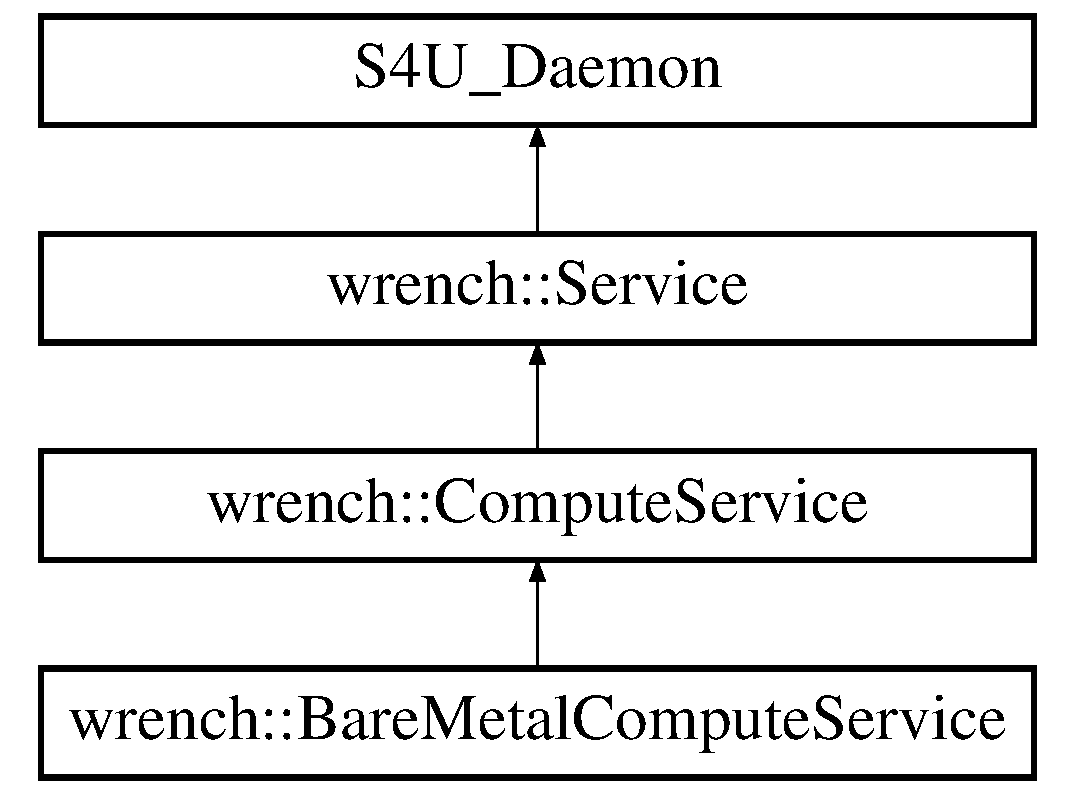
\includegraphics[height=4.000000cm]{classwrench_1_1_bare_metal_compute_service}
\end{center}
\end{figure}
\subsection*{Public Member Functions}
\begin{DoxyCompactItemize}
\item 
\hyperlink{classwrench_1_1_bare_metal_compute_service_ad1f0b74b15538742ec16da2f805df662}{Bare\+Metal\+Compute\+Service} (const std\+::string \&hostname, const std\+::map$<$ std\+::string, std\+::tuple$<$ unsigned long, double $>$$>$ compute\+\_\+resources, double scratch\+\_\+space\+\_\+size, std\+::map$<$ std\+::string, std\+::string $>$ property\+\_\+list=\{\}, std\+::map$<$ std\+::string, std\+::string $>$ messagepayload\+\_\+list=\{\})
\begin{DoxyCompactList}\small\item\em Constructor. \end{DoxyCompactList}\item 
\hyperlink{classwrench_1_1_bare_metal_compute_service_a67f03e4100d64ad6921dd65bfd1c8293}{Bare\+Metal\+Compute\+Service} (const std\+::string \&hostname, const std\+::set$<$ std\+::string $>$ compute\+\_\+hosts, double scratch\+\_\+space\+\_\+size, std\+::map$<$ std\+::string, std\+::string $>$ property\+\_\+list=\{\}, std\+::map$<$ std\+::string, std\+::string $>$ messagepayload\+\_\+list=\{\})
\begin{DoxyCompactList}\small\item\em Constructor. \end{DoxyCompactList}\end{DoxyCompactItemize}
\subsection*{Additional Inherited Members}


\subsection{Detailed Description}
A compute service that manages a set of multi-\/core compute hosts and provides access to their resources. 

One can think of this as a simple service that allows the user to run tasks and to specify for each task on which host it should run and with how many cores. If no host is specified, the service will pick the least loaded host. If no number of cores is specified, the service will use as many cores as possible. The service will make sure that the R\+AM capacity of a host is not exceeded by possibly delaying task executions until enough R\+AM is available. 

\subsection{Constructor \& Destructor Documentation}
\mbox{\Hypertarget{classwrench_1_1_bare_metal_compute_service_ad1f0b74b15538742ec16da2f805df662}\label{classwrench_1_1_bare_metal_compute_service_ad1f0b74b15538742ec16da2f805df662}} 
\index{wrench\+::\+Bare\+Metal\+Compute\+Service@{wrench\+::\+Bare\+Metal\+Compute\+Service}!Bare\+Metal\+Compute\+Service@{Bare\+Metal\+Compute\+Service}}
\index{Bare\+Metal\+Compute\+Service@{Bare\+Metal\+Compute\+Service}!wrench\+::\+Bare\+Metal\+Compute\+Service@{wrench\+::\+Bare\+Metal\+Compute\+Service}}
\subsubsection{\texorpdfstring{Bare\+Metal\+Compute\+Service()}{BareMetalComputeService()}\hspace{0.1cm}{\footnotesize\ttfamily [1/2]}}
{\footnotesize\ttfamily wrench\+::\+Bare\+Metal\+Compute\+Service\+::\+Bare\+Metal\+Compute\+Service (\begin{DoxyParamCaption}\item[{const std\+::string \&}]{hostname,  }\item[{const std\+::map$<$ std\+::string, std\+::tuple$<$ unsigned long, double $>$$>$}]{compute\+\_\+resources,  }\item[{double}]{scratch\+\_\+space\+\_\+size,  }\item[{std\+::map$<$ std\+::string, std\+::string $>$}]{property\+\_\+list = {\ttfamily \{\}},  }\item[{std\+::map$<$ std\+::string, std\+::string $>$}]{messagepayload\+\_\+list = {\ttfamily \{\}} }\end{DoxyParamCaption})}



Constructor. 


\begin{DoxyParams}{Parameters}
{\em hostname} & the name of the host on which the service should be started \\
\hline
{\em compute\+\_\+resources} & a map of $<$num\+\_\+cores, memory$>$ tuples, indexed by hostname, which represents the compute resources available to this service.
\begin{DoxyItemize}
\item use num\+\_\+cores = \hyperlink{classwrench_1_1_compute_service_a1160f521623440ad4e0e0823e08a7d22}{Compute\+Service\+::\+A\+L\+L\+\_\+\+C\+O\+R\+ES} to use all cores available on the host
\item use memory = \hyperlink{classwrench_1_1_compute_service_abc4fe0bad59f544b4b34d0e7d4012d44}{Compute\+Service\+::\+A\+L\+L\+\_\+\+R\+AM} to use all R\+AM available on the host 
\end{DoxyItemize}\\
\hline
{\em scratch\+\_\+space\+\_\+size} & size (in bytes) of the compute service\textquotesingle{}s scratch storage paste \\
\hline
{\em property\+\_\+list} & a property list (\{\} means \char`\"{}use all defaults\char`\"{}) \\
\hline
{\em messagepayload\+\_\+list} & a message payload list (\{\} means \char`\"{}use all defaults\char`\"{}) \\
\hline
\end{DoxyParams}
\mbox{\Hypertarget{classwrench_1_1_bare_metal_compute_service_a67f03e4100d64ad6921dd65bfd1c8293}\label{classwrench_1_1_bare_metal_compute_service_a67f03e4100d64ad6921dd65bfd1c8293}} 
\index{wrench\+::\+Bare\+Metal\+Compute\+Service@{wrench\+::\+Bare\+Metal\+Compute\+Service}!Bare\+Metal\+Compute\+Service@{Bare\+Metal\+Compute\+Service}}
\index{Bare\+Metal\+Compute\+Service@{Bare\+Metal\+Compute\+Service}!wrench\+::\+Bare\+Metal\+Compute\+Service@{wrench\+::\+Bare\+Metal\+Compute\+Service}}
\subsubsection{\texorpdfstring{Bare\+Metal\+Compute\+Service()}{BareMetalComputeService()}\hspace{0.1cm}{\footnotesize\ttfamily [2/2]}}
{\footnotesize\ttfamily wrench\+::\+Bare\+Metal\+Compute\+Service\+::\+Bare\+Metal\+Compute\+Service (\begin{DoxyParamCaption}\item[{const std\+::string \&}]{hostname,  }\item[{const std\+::set$<$ std\+::string $>$}]{compute\+\_\+hosts,  }\item[{double}]{scratch\+\_\+space\+\_\+size,  }\item[{std\+::map$<$ std\+::string, std\+::string $>$}]{property\+\_\+list = {\ttfamily \{\}},  }\item[{std\+::map$<$ std\+::string, std\+::string $>$}]{messagepayload\+\_\+list = {\ttfamily \{\}} }\end{DoxyParamCaption})}



Constructor. 


\begin{DoxyParams}{Parameters}
{\em hostname} & the name of the host on which the service should be started \\
\hline
{\em compute\+\_\+hosts,\+:} & the names of the hosts available as compute resources (the service will use all the cores and all the R\+AM of each host) \\
\hline
{\em scratch\+\_\+space\+\_\+size} & size (in bytes) of the compute service\textquotesingle{}s scratch storage paste \\
\hline
{\em property\+\_\+list} & a property list (\{\} means \char`\"{}use all defaults\char`\"{}) \\
\hline
{\em messagepayload\+\_\+list} & a message payload list (\{\} means \char`\"{}use all defaults\char`\"{}) \\
\hline
\end{DoxyParams}


The documentation for this class was generated from the following files\+:\begin{DoxyCompactItemize}
\item 
/\+Users/rafsilva/\+Documents/isi/workspace/wrench/wrench/include/wrench/services/compute/bare\+\_\+metal/Bare\+Metal\+Compute\+Service.\+h\item 
/\+Users/rafsilva/\+Documents/isi/workspace/wrench/wrench/src/wrench/services/compute/bare\+\_\+metal/Bare\+Metal\+Compute\+Service.\+cpp\end{DoxyCompactItemize}

\hypertarget{classwrench_1_1_bare_metal_compute_service_message_payload}{}\section{wrench\+:\+:Bare\+Metal\+Compute\+Service\+Message\+Payload Class Reference}
\label{classwrench_1_1_bare_metal_compute_service_message_payload}\index{wrench\+::\+Bare\+Metal\+Compute\+Service\+Message\+Payload@{wrench\+::\+Bare\+Metal\+Compute\+Service\+Message\+Payload}}


Configurable message payloads for a Multi\+Host\+Multicore\+Compute\+Service.  




{\ttfamily \#include $<$Bare\+Metal\+Compute\+Service\+Message\+Payload.\+h$>$}

Inheritance diagram for wrench\+:\+:Bare\+Metal\+Compute\+Service\+Message\+Payload\+:\begin{figure}[H]
\begin{center}
\leavevmode
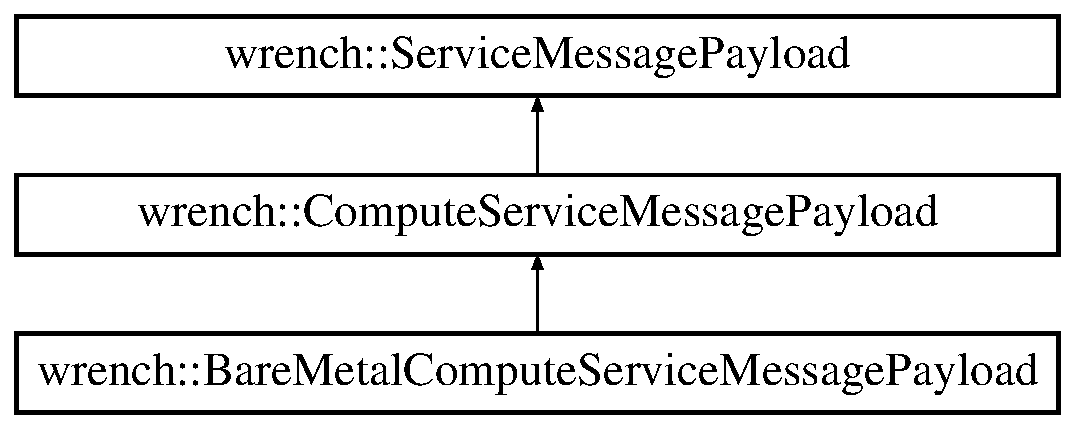
\includegraphics[height=3.000000cm]{classwrench_1_1_bare_metal_compute_service_message_payload}
\end{center}
\end{figure}
\subsection*{Static Public Attributes}
\begin{DoxyCompactItemize}
\item 
\mbox{\Hypertarget{classwrench_1_1_bare_metal_compute_service_message_payload_a10eabc33f0fc2110737b3cf151623250}\label{classwrench_1_1_bare_metal_compute_service_message_payload_a10eabc33f0fc2110737b3cf151623250}} 
static const std\+::string \hyperlink{classwrench_1_1_bare_metal_compute_service_message_payload_a10eabc33f0fc2110737b3cf151623250}{F\+L\+O\+P\+\_\+\+R\+A\+T\+E\+\_\+\+A\+N\+S\+W\+E\+R\+\_\+\+M\+E\+S\+S\+A\+G\+E\+\_\+\+P\+A\+Y\+L\+O\+AD}
\begin{DoxyCompactList}\small\item\em The number of bytes in the control message sent by the daemon to state its per-\/core flop rate. \end{DoxyCompactList}\item 
\mbox{\Hypertarget{classwrench_1_1_bare_metal_compute_service_message_payload_a1ab951377c6247c9b58c0f4494cf2950}\label{classwrench_1_1_bare_metal_compute_service_message_payload_a1ab951377c6247c9b58c0f4494cf2950}} 
static const std\+::string \hyperlink{classwrench_1_1_bare_metal_compute_service_message_payload_a1ab951377c6247c9b58c0f4494cf2950}{F\+L\+O\+P\+\_\+\+R\+A\+T\+E\+\_\+\+R\+E\+Q\+U\+E\+S\+T\+\_\+\+M\+E\+S\+S\+A\+G\+E\+\_\+\+P\+A\+Y\+L\+O\+AD}
\begin{DoxyCompactList}\small\item\em The number of bytes in the control message sent to the daemon to ask it for its per-\/core flop rate. \end{DoxyCompactList}\item 
\mbox{\Hypertarget{classwrench_1_1_bare_metal_compute_service_message_payload_ae7c1a15d40447d30f00bee194929fd70}\label{classwrench_1_1_bare_metal_compute_service_message_payload_ae7c1a15d40447d30f00bee194929fd70}} 
static const std\+::string \hyperlink{classwrench_1_1_bare_metal_compute_service_message_payload_ae7c1a15d40447d30f00bee194929fd70}{N\+O\+T\+\_\+\+E\+N\+O\+U\+G\+H\+\_\+\+C\+O\+R\+E\+S\+\_\+\+M\+E\+S\+S\+A\+G\+E\+\_\+\+P\+A\+Y\+L\+O\+AD}
\begin{DoxyCompactList}\small\item\em The number of bytes in the control message sent by the daemon to state that it does not have sufficient cores to (ever) run a submitted job. \end{DoxyCompactList}\end{DoxyCompactItemize}


\subsection{Detailed Description}
Configurable message payloads for a Multi\+Host\+Multicore\+Compute\+Service. 

The documentation for this class was generated from the following file\+:\begin{DoxyCompactItemize}
\item 
/\+Users/rafsilva/\+Documents/isi/workspace/wrench/wrench/include/wrench/services/compute/bare\+\_\+metal/Bare\+Metal\+Compute\+Service\+Message\+Payload.\+h\end{DoxyCompactItemize}

\hypertarget{classwrench_1_1_bare_metal_compute_service_property}{}\section{wrench\+:\+:Bare\+Metal\+Compute\+Service\+Property Class Reference}
\label{classwrench_1_1_bare_metal_compute_service_property}\index{wrench\+::\+Bare\+Metal\+Compute\+Service\+Property@{wrench\+::\+Bare\+Metal\+Compute\+Service\+Property}}


Configurable properties for a Multi\+Host\+Multicore\+Compute\+Service.  




{\ttfamily \#include $<$Bare\+Metal\+Compute\+Service\+Property.\+h$>$}

Inheritance diagram for wrench\+:\+:Bare\+Metal\+Compute\+Service\+Property\+:\begin{figure}[H]
\begin{center}
\leavevmode
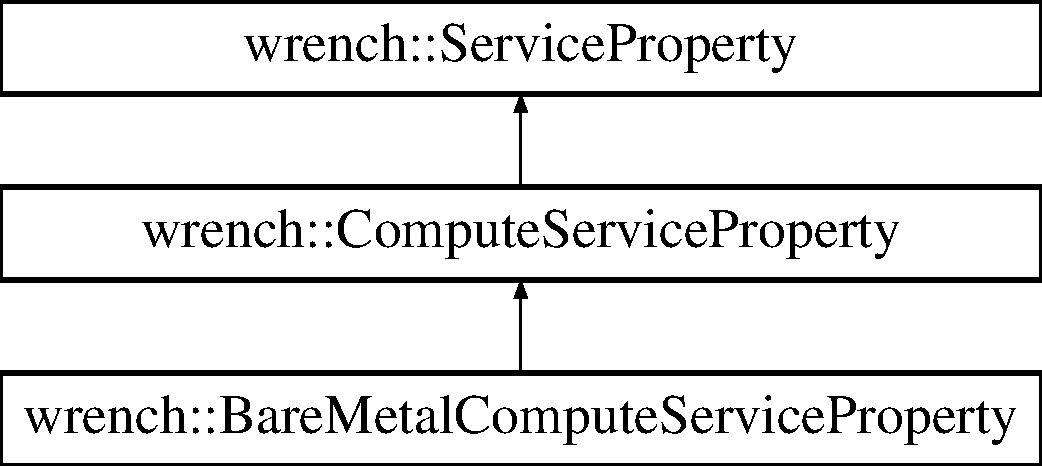
\includegraphics[height=3.000000cm]{classwrench_1_1_bare_metal_compute_service_property}
\end{center}
\end{figure}
\subsection*{Static Public Attributes}
\begin{DoxyCompactItemize}
\item 
\mbox{\Hypertarget{classwrench_1_1_bare_metal_compute_service_property_a63dfaa7ebb4dc18d236c58384f14dd25}\label{classwrench_1_1_bare_metal_compute_service_property_a63dfaa7ebb4dc18d236c58384f14dd25}} 
static const std\+::string \hyperlink{classwrench_1_1_bare_metal_compute_service_property_a63dfaa7ebb4dc18d236c58384f14dd25}{T\+H\+R\+E\+A\+D\+\_\+\+S\+T\+A\+R\+T\+U\+P\+\_\+\+O\+V\+E\+R\+H\+E\+AD}
\begin{DoxyCompactList}\small\item\em The overhead to start a thread, in seconds. \end{DoxyCompactList}\end{DoxyCompactItemize}


\subsection{Detailed Description}
Configurable properties for a Multi\+Host\+Multicore\+Compute\+Service. 

The documentation for this class was generated from the following file\+:\begin{DoxyCompactItemize}
\item 
/\+Users/rafsilva/\+Documents/isi/workspace/wrench/wrench/include/wrench/services/compute/bare\+\_\+metal/Bare\+Metal\+Compute\+Service\+Property.\+h\end{DoxyCompactItemize}

\hypertarget{classwrench_1_1_batch_service}{}\section{wrench\+:\+:Batch\+Service Class Reference}
\label{classwrench_1_1_batch_service}\index{wrench\+::\+Batch\+Service@{wrench\+::\+Batch\+Service}}


A batch-\/scheduled compute service that manages a set of compute hosts and controls access to their resource via a batch queue.  




{\ttfamily \#include $<$Batch\+Service.\+h$>$}

Inheritance diagram for wrench\+:\+:Batch\+Service\+:\begin{figure}[H]
\begin{center}
\leavevmode
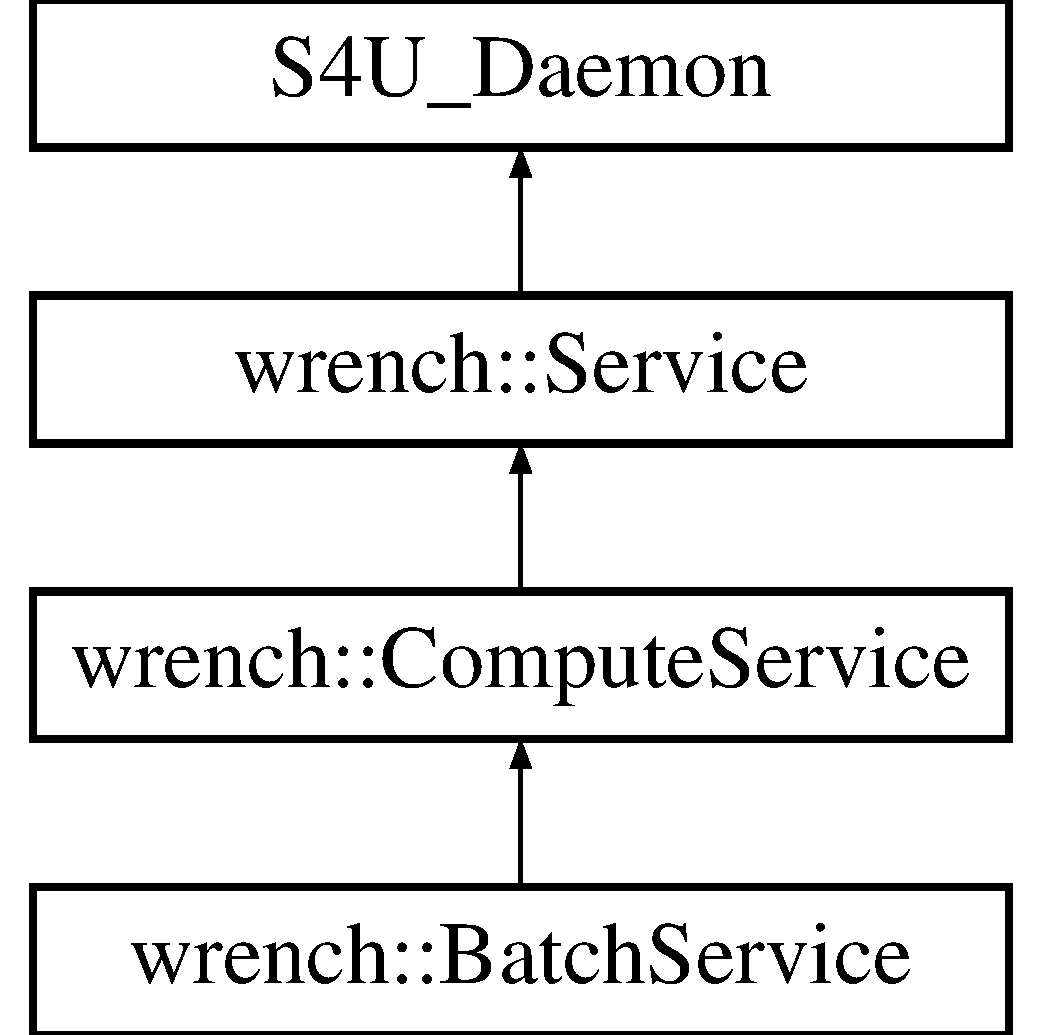
\includegraphics[height=4.000000cm]{classwrench_1_1_batch_service}
\end{center}
\end{figure}
\subsection*{Public Member Functions}
\begin{DoxyCompactItemize}
\item 
\hyperlink{classwrench_1_1_batch_service_a2f91405c977001fa52acda0fe849f143}{Batch\+Service} (std\+::string \&hostname, std\+::vector$<$ std\+::string $>$ compute\+\_\+hosts, double scratch\+\_\+space\+\_\+size, std\+::map$<$ std\+::string, std\+::string $>$ property\+\_\+list=\{\}, std\+::map$<$ std\+::string, std\+::string $>$ messagepayload\+\_\+list=\{\})
\begin{DoxyCompactList}\small\item\em Constructor. \end{DoxyCompactList}\end{DoxyCompactItemize}
\subsection*{Additional Inherited Members}


\subsection{Detailed Description}
A batch-\/scheduled compute service that manages a set of compute hosts and controls access to their resource via a batch queue. 

In the current implementation of this service, like for many of its real-\/world counterparts, memory partitioning among jobs on the same host is not handled. When multiple jobs share hosts, which can happen when jobs require only a few cores per host and can thus be co-\/located on the same hosts in a non-\/exclusive fashion, each job simply runs as if it had access to the full R\+AM of each compute host it is scheduled on. The simulation of these memory contended scenarios is thus, for now, not realistic as there is no simulation of the effects of memory sharing (e.\+g., swapping). 

\subsection{Constructor \& Destructor Documentation}
\mbox{\Hypertarget{classwrench_1_1_batch_service_a2f91405c977001fa52acda0fe849f143}\label{classwrench_1_1_batch_service_a2f91405c977001fa52acda0fe849f143}} 
\index{wrench\+::\+Batch\+Service@{wrench\+::\+Batch\+Service}!Batch\+Service@{Batch\+Service}}
\index{Batch\+Service@{Batch\+Service}!wrench\+::\+Batch\+Service@{wrench\+::\+Batch\+Service}}
\subsubsection{\texorpdfstring{Batch\+Service()}{BatchService()}}
{\footnotesize\ttfamily wrench\+::\+Batch\+Service\+::\+Batch\+Service (\begin{DoxyParamCaption}\item[{std\+::string \&}]{hostname,  }\item[{std\+::vector$<$ std\+::string $>$}]{compute\+\_\+hosts,  }\item[{double}]{scratch\+\_\+space\+\_\+size,  }\item[{std\+::map$<$ std\+::string, std\+::string $>$}]{property\+\_\+list = {\ttfamily \{\}},  }\item[{std\+::map$<$ std\+::string, std\+::string $>$}]{messagepayload\+\_\+list = {\ttfamily \{\}} }\end{DoxyParamCaption})}



Constructor. 


\begin{DoxyParams}{Parameters}
{\em hostname} & the hostname on which to start the service \\
\hline
{\em compute\+\_\+hosts} & the list of names of the available compute hosts
\begin{DoxyItemize}
\item the hosts must be homogeneous (speed, number of cores, and R\+AM size)
\item all cores are usable by the batch service on each host
\item all R\+AM is usable by the batch service on each host 
\end{DoxyItemize}\\
\hline
{\em scratch\+\_\+space\+\_\+size} & the size for the scratch storage space for the service (0 means \char`\"{}no scratch space\char`\"{}) \\
\hline
{\em property\+\_\+list} & a property list that specifies \hyperlink{classwrench_1_1_batch_service_property}{Batch\+Service\+Property} values (\{\} means \char`\"{}use all defaults\char`\"{}) \\
\hline
{\em messagepayload\+\_\+list} & a message payload list that specifies \hyperlink{classwrench_1_1_batch_service_message_payload}{Batch\+Service\+Message\+Payload} values (\{\} means \char`\"{}use all defaults\char`\"{}) \\
\hline
\end{DoxyParams}


The documentation for this class was generated from the following files\+:\begin{DoxyCompactItemize}
\item 
/\+Users/rafsilva/\+Documents/isi/workspace/wrench/wrench/include/wrench/services/compute/batch/Batch\+Service.\+h\item 
/\+Users/rafsilva/\+Documents/isi/workspace/wrench/wrench/src/wrench/services/compute/batch/Batch\+Service.\+cpp\end{DoxyCompactItemize}

\hypertarget{classwrench_1_1_batch_service_message_payload}{}\section{wrench\+:\+:Batch\+Service\+Message\+Payload Class Reference}
\label{classwrench_1_1_batch_service_message_payload}\index{wrench\+::\+Batch\+Service\+Message\+Payload@{wrench\+::\+Batch\+Service\+Message\+Payload}}


Configurable message payloads for a \hyperlink{classwrench_1_1_batch_service}{Batch\+Service}.  




{\ttfamily \#include $<$Batch\+Service\+Message\+Payload.\+h$>$}

Inheritance diagram for wrench\+:\+:Batch\+Service\+Message\+Payload\+:\begin{figure}[H]
\begin{center}
\leavevmode
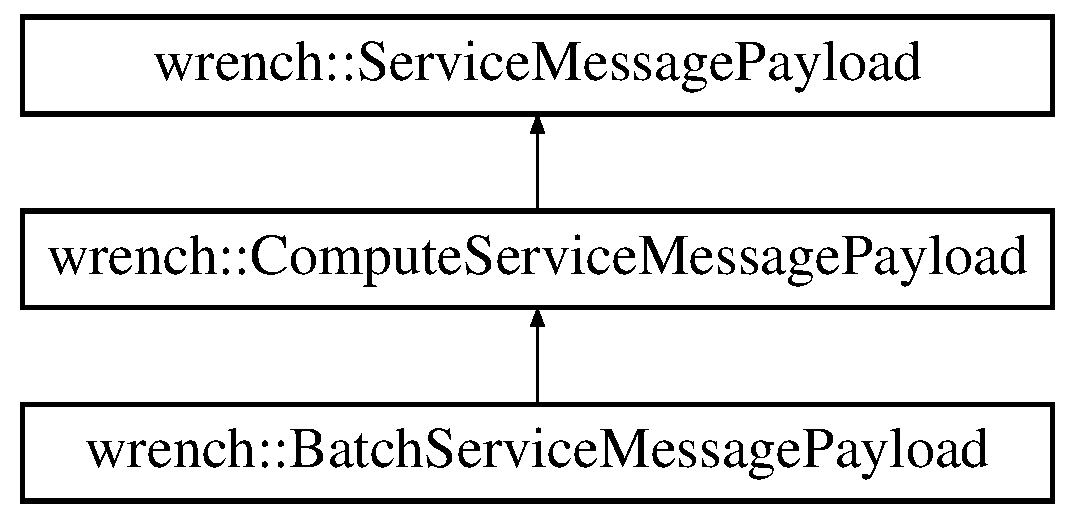
\includegraphics[height=3.000000cm]{classwrench_1_1_batch_service_message_payload}
\end{center}
\end{figure}
\subsection*{Additional Inherited Members}


\subsection{Detailed Description}
Configurable message payloads for a \hyperlink{classwrench_1_1_batch_service}{Batch\+Service}. 

The documentation for this class was generated from the following file\+:\begin{DoxyCompactItemize}
\item 
/\+Users/rafsilva/\+Documents/isi/workspace/wrench/wrench/include/wrench/services/compute/batch/Batch\+Service\+Message\+Payload.\+h\end{DoxyCompactItemize}

\hypertarget{classwrench_1_1_batch_service_property}{}\section{wrench\+:\+:Batch\+Service\+Property Class Reference}
\label{classwrench_1_1_batch_service_property}\index{wrench\+::\+Batch\+Service\+Property@{wrench\+::\+Batch\+Service\+Property}}


Configurable properties for a \hyperlink{classwrench_1_1_batch_service}{Batch\+Service}.  




{\ttfamily \#include $<$Batch\+Service\+Property.\+h$>$}

Inheritance diagram for wrench\+:\+:Batch\+Service\+Property\+:\begin{figure}[H]
\begin{center}
\leavevmode
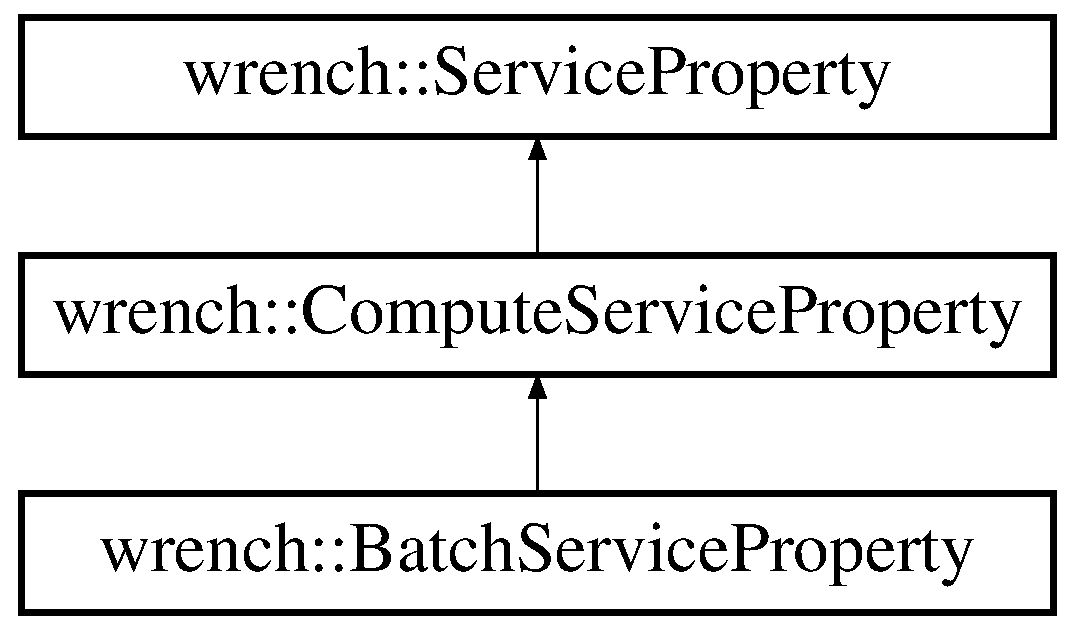
\includegraphics[height=3.000000cm]{classwrench_1_1_batch_service_property}
\end{center}
\end{figure}
\subsection*{Static Public Attributes}
\begin{DoxyCompactItemize}
\item 
static const std\+::string \hyperlink{classwrench_1_1_batch_service_property_a51cc79b2c963a67dac5685fbba4e5a9f}{B\+A\+T\+C\+H\+\_\+\+Q\+U\+E\+U\+E\+\_\+\+O\+R\+D\+E\+R\+I\+N\+G\+\_\+\+A\+L\+G\+O\+R\+I\+T\+HM}
\begin{DoxyCompactList}\small\item\em The batch queue ordering algorithm. Can be\+: \end{DoxyCompactList}\item 
\mbox{\Hypertarget{classwrench_1_1_batch_service_property_a685c9784445ed28adbe43f69ccb98249}\label{classwrench_1_1_batch_service_property_a685c9784445ed28adbe43f69ccb98249}} 
static const std\+::string \hyperlink{classwrench_1_1_batch_service_property_a685c9784445ed28adbe43f69ccb98249}{B\+A\+T\+C\+H\+\_\+\+R\+J\+M\+S\+\_\+\+D\+E\+L\+AY}
\begin{DoxyCompactList}\small\item\em Number of seconds that the Batch Scheduler adds to the runtime of each incoming job. This is something production batch systems do to avoid too aggressive job terminations. For instance, if a job says it wants to run for (at most) 60 seconds, the system will actually assume the job wants to run for (at most) 60 + 5 seconds. \end{DoxyCompactList}\item 
static const std\+::string \hyperlink{classwrench_1_1_batch_service_property_aceb0af1c33f5ff2da347f54a484ce32e}{B\+A\+T\+C\+H\+\_\+\+S\+C\+H\+E\+D\+U\+L\+I\+N\+G\+\_\+\+A\+L\+G\+O\+R\+I\+T\+HM}
\begin{DoxyCompactList}\small\item\em The batch scheduling algorithm. Can be\+: \end{DoxyCompactList}\item 
static const std\+::string \hyperlink{classwrench_1_1_batch_service_property_ac21c68a5a297ba00fc919cec0d90c18d}{B\+A\+T\+S\+C\+H\+E\+D\+\_\+\+C\+O\+N\+T\+I\+G\+U\+O\+U\+S\+\_\+\+A\+L\+L\+O\+C\+A\+T\+I\+ON}
\begin{DoxyCompactList}\small\item\em Controls Batsched node allocation policy. \end{DoxyCompactList}\item 
static const std\+::string \hyperlink{classwrench_1_1_batch_service_property_aaab42384419440aacdbaac79e3346bf1}{B\+A\+T\+S\+C\+H\+E\+D\+\_\+\+L\+O\+G\+G\+I\+N\+G\+\_\+\+M\+U\+T\+ED}
\begin{DoxyCompactList}\small\item\em Controls Batsched logging. \end{DoxyCompactList}\item 
static const std\+::string \hyperlink{classwrench_1_1_batch_service_property_af75bbbe70a733d3a65cddc5c57b0b441}{H\+O\+S\+T\+\_\+\+S\+E\+L\+E\+C\+T\+I\+O\+N\+\_\+\+A\+L\+G\+O\+R\+I\+T\+HM}
\begin{DoxyCompactList}\small\item\em The host selection algorithm. Can be\+: \end{DoxyCompactList}\item 
static const std\+::string \hyperlink{classwrench_1_1_batch_service_property_a0757979b1512be80fda90cbab946b51f}{O\+U\+T\+P\+U\+T\+\_\+\+C\+S\+V\+\_\+\+J\+O\+B\+\_\+\+L\+OG}
\begin{DoxyCompactList}\small\item\em Path to a to-\/be-\/generated Batsim-\/style C\+SV trace file (e.\+g. for b3atch schedule visualization purposes). \end{DoxyCompactList}\item 
\mbox{\Hypertarget{classwrench_1_1_batch_service_property_a0bde5c75f5f093ae15e68d67ae453ac3}\label{classwrench_1_1_batch_service_property_a0bde5c75f5f093ae15e68d67ae453ac3}} 
static const std\+::string \hyperlink{classwrench_1_1_batch_service_property_a0bde5c75f5f093ae15e68d67ae453ac3}{S\+I\+M\+U\+L\+A\+T\+E\+\_\+\+C\+O\+M\+P\+U\+T\+A\+T\+I\+O\+N\+\_\+\+A\+S\+\_\+\+S\+L\+E\+EP}
\begin{DoxyCompactList}\small\item\em Simulate computation as just a sleep instead of an actual comput thread. This is for scalability reason, and only simulation-\/valid if one is sure that cores are space shared (i.\+e., only a single compute thread can ever run on a core at once). Since space-\/sharing at the core level is typically the case in batch-\/scheduled clusters, this is likely fine. Possible values are \char`\"{}false\char`\"{} (the default) or \char`\"{}true\char`\"{}. \end{DoxyCompactList}\item 
\mbox{\Hypertarget{classwrench_1_1_batch_service_property_a6a7fb4d9f505cc29f7236ea3e5713f34}\label{classwrench_1_1_batch_service_property_a6a7fb4d9f505cc29f7236ea3e5713f34}} 
static const std\+::string \hyperlink{classwrench_1_1_batch_service_property_a6a7fb4d9f505cc29f7236ea3e5713f34}{S\+I\+M\+U\+L\+A\+T\+E\+D\+\_\+\+W\+O\+R\+K\+L\+O\+A\+D\+\_\+\+T\+R\+A\+C\+E\+\_\+\+F\+I\+LE}
\begin{DoxyCompactList}\small\item\em Path to a workload trace file to be replayed. The trace file can be be in the S\+WF format (see \href{http://www.cs.huji.ac.il/labs/parallel/workload/swf.html}{\tt http\+://www.\+cs.\+huji.\+ac.\+il/labs/parallel/workload/swf.\+html}), in which case it must have extension \char`\"{}.\+swf\char`\"{}, or in the J\+S\+ON format as used in the B\+A\+T\+S\+IM project (see \href{https://github.com/oar-team/batsim}{\tt https\+://github.\+com/oar-\/team/batsim}), in which case is must have the \char`\"{}.\+json\char`\"{} extension). The jobs in the trace whose node/host/processor/core requirements exceed the capacity of the batch service will simply be capped at that capacity. Job submission times in the trace files are relative to the \hyperlink{classwrench_1_1_batch_service}{Batch\+Service}\textquotesingle{}s start time (i.\+e., all jobs in the trace files will be replayed no matter when the \hyperlink{classwrench_1_1_batch_service}{Batch\+Service} starts). Note that in the B\+A\+T\+S\+IM J\+S\+ON format, the trace does not contains requested vs. actual trace runtimes, and to all requested runtimes are 100\% accurate. \end{DoxyCompactList}\item 
static const std\+::string \hyperlink{classwrench_1_1_batch_service_property_a3869070a4dcfeea63bb5f9a8518de1cc}{T\+A\+S\+K\+\_\+\+S\+E\+L\+E\+C\+T\+I\+O\+N\+\_\+\+A\+L\+G\+O\+R\+I\+T\+HM}
\begin{DoxyCompactList}\small\item\em The algorithm to pick which ready computational task (within a standard job executed by the batch service), in case multiple tasks are ready, should run first. This is typically not managed by a batch scheduler, but by some application-\/level script that executes a set of tasks within compute resources allocated by the batch scheduler. Possible values are\+: \end{DoxyCompactList}\item 
\mbox{\Hypertarget{classwrench_1_1_batch_service_property_ad60a71526e251e20cbd871e5d30e5023}\label{classwrench_1_1_batch_service_property_ad60a71526e251e20cbd871e5d30e5023}} 
static const std\+::string \hyperlink{classwrench_1_1_batch_service_property_ad60a71526e251e20cbd871e5d30e5023}{T\+H\+R\+E\+A\+D\+\_\+\+S\+T\+A\+R\+T\+U\+P\+\_\+\+O\+V\+E\+R\+H\+E\+AD}
\begin{DoxyCompactList}\small\item\em The overhead to start a thread execution, in seconds. \end{DoxyCompactList}\item 
static const std\+::string \hyperlink{classwrench_1_1_batch_service_property_a5f40d6321b3062091d00db8a5a9dc07e}{U\+S\+E\+\_\+\+R\+E\+A\+L\+\_\+\+R\+U\+N\+T\+I\+M\+E\+S\+\_\+\+A\+S\+\_\+\+R\+E\+Q\+U\+E\+S\+T\+E\+D\+\_\+\+R\+U\+N\+T\+I\+M\+ES}
\begin{DoxyCompactList}\small\item\em Whether, when simulating a workload trace file, to use the actual runtimes as requested runtimes (i.\+e., simulating users who request exactly what they need) or not (i.\+e., simulating users who always overestimate what they need, which is typical in the real world)\+: \end{DoxyCompactList}\end{DoxyCompactItemize}


\subsection{Detailed Description}
Configurable properties for a \hyperlink{classwrench_1_1_batch_service}{Batch\+Service}. 

\subsection{Member Data Documentation}
\mbox{\Hypertarget{classwrench_1_1_batch_service_property_a51cc79b2c963a67dac5685fbba4e5a9f}\label{classwrench_1_1_batch_service_property_a51cc79b2c963a67dac5685fbba4e5a9f}} 
\index{wrench\+::\+Batch\+Service\+Property@{wrench\+::\+Batch\+Service\+Property}!B\+A\+T\+C\+H\+\_\+\+Q\+U\+E\+U\+E\+\_\+\+O\+R\+D\+E\+R\+I\+N\+G\+\_\+\+A\+L\+G\+O\+R\+I\+T\+HM@{B\+A\+T\+C\+H\+\_\+\+Q\+U\+E\+U\+E\+\_\+\+O\+R\+D\+E\+R\+I\+N\+G\+\_\+\+A\+L\+G\+O\+R\+I\+T\+HM}}
\index{B\+A\+T\+C\+H\+\_\+\+Q\+U\+E\+U\+E\+\_\+\+O\+R\+D\+E\+R\+I\+N\+G\+\_\+\+A\+L\+G\+O\+R\+I\+T\+HM@{B\+A\+T\+C\+H\+\_\+\+Q\+U\+E\+U\+E\+\_\+\+O\+R\+D\+E\+R\+I\+N\+G\+\_\+\+A\+L\+G\+O\+R\+I\+T\+HM}!wrench\+::\+Batch\+Service\+Property@{wrench\+::\+Batch\+Service\+Property}}
\subsubsection{\texorpdfstring{B\+A\+T\+C\+H\+\_\+\+Q\+U\+E\+U\+E\+\_\+\+O\+R\+D\+E\+R\+I\+N\+G\+\_\+\+A\+L\+G\+O\+R\+I\+T\+HM}{BATCH\_QUEUE\_ORDERING\_ALGORITHM}}
{\footnotesize\ttfamily const std\+::string wrench\+::\+Batch\+Service\+Property\+::\+B\+A\+T\+C\+H\+\_\+\+Q\+U\+E\+U\+E\+\_\+\+O\+R\+D\+E\+R\+I\+N\+G\+\_\+\+A\+L\+G\+O\+R\+I\+T\+HM\hspace{0.3cm}{\ttfamily [static]}}



The batch queue ordering algorithm. Can be\+: 


\begin{DoxyItemize}
\item If E\+N\+A\+B\+L\+E\+\_\+\+B\+A\+T\+S\+C\+H\+ED is set to off / not set\+: ignored
\item If E\+N\+A\+B\+L\+E\+\_\+\+B\+A\+T\+S\+C\+H\+ED is set to on\+:
\begin{DoxyItemize}
\item whatever queue ordering algorithm is supported by Batsched (by default\+: \char`\"{}fcfs\char`\"{}) 
\end{DoxyItemize}
\end{DoxyItemize}\mbox{\Hypertarget{classwrench_1_1_batch_service_property_aceb0af1c33f5ff2da347f54a484ce32e}\label{classwrench_1_1_batch_service_property_aceb0af1c33f5ff2da347f54a484ce32e}} 
\index{wrench\+::\+Batch\+Service\+Property@{wrench\+::\+Batch\+Service\+Property}!B\+A\+T\+C\+H\+\_\+\+S\+C\+H\+E\+D\+U\+L\+I\+N\+G\+\_\+\+A\+L\+G\+O\+R\+I\+T\+HM@{B\+A\+T\+C\+H\+\_\+\+S\+C\+H\+E\+D\+U\+L\+I\+N\+G\+\_\+\+A\+L\+G\+O\+R\+I\+T\+HM}}
\index{B\+A\+T\+C\+H\+\_\+\+S\+C\+H\+E\+D\+U\+L\+I\+N\+G\+\_\+\+A\+L\+G\+O\+R\+I\+T\+HM@{B\+A\+T\+C\+H\+\_\+\+S\+C\+H\+E\+D\+U\+L\+I\+N\+G\+\_\+\+A\+L\+G\+O\+R\+I\+T\+HM}!wrench\+::\+Batch\+Service\+Property@{wrench\+::\+Batch\+Service\+Property}}
\subsubsection{\texorpdfstring{B\+A\+T\+C\+H\+\_\+\+S\+C\+H\+E\+D\+U\+L\+I\+N\+G\+\_\+\+A\+L\+G\+O\+R\+I\+T\+HM}{BATCH\_SCHEDULING\_ALGORITHM}}
{\footnotesize\ttfamily const std\+::string wrench\+::\+Batch\+Service\+Property\+::\+B\+A\+T\+C\+H\+\_\+\+S\+C\+H\+E\+D\+U\+L\+I\+N\+G\+\_\+\+A\+L\+G\+O\+R\+I\+T\+HM\hspace{0.3cm}{\ttfamily [static]}}



The batch scheduling algorithm. Can be\+: 


\begin{DoxyItemize}
\item If E\+N\+A\+B\+L\+E\+\_\+\+B\+A\+T\+S\+C\+H\+ED is set to off / not set\+:
\begin{DoxyItemize}
\item \char`\"{}\+F\+C\+F\+S\char`\"{}\+: First Come First Serve
\end{DoxyItemize}
\item If E\+N\+A\+B\+L\+E\+\_\+\+B\+A\+T\+S\+C\+H\+ED is set to on\+:
\begin{DoxyItemize}
\item whatever scheduling algorithm is supported by Batsched (by default\+: \char`\"{}conservative\+\_\+bf\char`\"{}, other options include \char`\"{}easy\+\_\+bf\char`\"{} and \char`\"{}easy\+\_\+bf\+\_\+fast\char`\"{}) 
\end{DoxyItemize}
\end{DoxyItemize}\mbox{\Hypertarget{classwrench_1_1_batch_service_property_ac21c68a5a297ba00fc919cec0d90c18d}\label{classwrench_1_1_batch_service_property_ac21c68a5a297ba00fc919cec0d90c18d}} 
\index{wrench\+::\+Batch\+Service\+Property@{wrench\+::\+Batch\+Service\+Property}!B\+A\+T\+S\+C\+H\+E\+D\+\_\+\+C\+O\+N\+T\+I\+G\+U\+O\+U\+S\+\_\+\+A\+L\+L\+O\+C\+A\+T\+I\+ON@{B\+A\+T\+S\+C\+H\+E\+D\+\_\+\+C\+O\+N\+T\+I\+G\+U\+O\+U\+S\+\_\+\+A\+L\+L\+O\+C\+A\+T\+I\+ON}}
\index{B\+A\+T\+S\+C\+H\+E\+D\+\_\+\+C\+O\+N\+T\+I\+G\+U\+O\+U\+S\+\_\+\+A\+L\+L\+O\+C\+A\+T\+I\+ON@{B\+A\+T\+S\+C\+H\+E\+D\+\_\+\+C\+O\+N\+T\+I\+G\+U\+O\+U\+S\+\_\+\+A\+L\+L\+O\+C\+A\+T\+I\+ON}!wrench\+::\+Batch\+Service\+Property@{wrench\+::\+Batch\+Service\+Property}}
\subsubsection{\texorpdfstring{B\+A\+T\+S\+C\+H\+E\+D\+\_\+\+C\+O\+N\+T\+I\+G\+U\+O\+U\+S\+\_\+\+A\+L\+L\+O\+C\+A\+T\+I\+ON}{BATSCHED\_CONTIGUOUS\_ALLOCATION}}
{\footnotesize\ttfamily const std\+::string wrench\+::\+Batch\+Service\+Property\+::\+B\+A\+T\+S\+C\+H\+E\+D\+\_\+\+C\+O\+N\+T\+I\+G\+U\+O\+U\+S\+\_\+\+A\+L\+L\+O\+C\+A\+T\+I\+ON\hspace{0.3cm}{\ttfamily [static]}}



Controls Batsched node allocation policy. 


\begin{DoxyItemize}
\item If E\+N\+A\+B\+L\+E\+\_\+\+B\+A\+T\+S\+C\+H\+ED is set to off or not set\+: ignored
\item If E\+N\+A\+B\+L\+E\+\_\+\+B\+A\+T\+S\+C\+H\+ED is set to on\+:
\begin{DoxyItemize}
\item \char`\"{}false\char`\"{}\+: do not enforce contiguous nodes for allocations (default)
\item \char`\"{}true\char`\"{}\+: enforce contiguous nodes for allocations (note that not all algorithms implemented by batsched support contiguous allocations, so this option may have no effect in some cases). 
\end{DoxyItemize}
\end{DoxyItemize}\mbox{\Hypertarget{classwrench_1_1_batch_service_property_aaab42384419440aacdbaac79e3346bf1}\label{classwrench_1_1_batch_service_property_aaab42384419440aacdbaac79e3346bf1}} 
\index{wrench\+::\+Batch\+Service\+Property@{wrench\+::\+Batch\+Service\+Property}!B\+A\+T\+S\+C\+H\+E\+D\+\_\+\+L\+O\+G\+G\+I\+N\+G\+\_\+\+M\+U\+T\+ED@{B\+A\+T\+S\+C\+H\+E\+D\+\_\+\+L\+O\+G\+G\+I\+N\+G\+\_\+\+M\+U\+T\+ED}}
\index{B\+A\+T\+S\+C\+H\+E\+D\+\_\+\+L\+O\+G\+G\+I\+N\+G\+\_\+\+M\+U\+T\+ED@{B\+A\+T\+S\+C\+H\+E\+D\+\_\+\+L\+O\+G\+G\+I\+N\+G\+\_\+\+M\+U\+T\+ED}!wrench\+::\+Batch\+Service\+Property@{wrench\+::\+Batch\+Service\+Property}}
\subsubsection{\texorpdfstring{B\+A\+T\+S\+C\+H\+E\+D\+\_\+\+L\+O\+G\+G\+I\+N\+G\+\_\+\+M\+U\+T\+ED}{BATSCHED\_LOGGING\_MUTED}}
{\footnotesize\ttfamily const std\+::string wrench\+::\+Batch\+Service\+Property\+::\+B\+A\+T\+S\+C\+H\+E\+D\+\_\+\+L\+O\+G\+G\+I\+N\+G\+\_\+\+M\+U\+T\+ED\hspace{0.3cm}{\ttfamily [static]}}



Controls Batsched logging. 


\begin{DoxyItemize}
\item If E\+N\+A\+B\+L\+E\+\_\+\+B\+A\+T\+S\+C\+H\+ED is set to off or not set\+: ignored
\item If E\+N\+A\+B\+L\+E\+\_\+\+B\+A\+T\+S\+C\+H\+ED is set to on\+:
\begin{DoxyItemize}
\item \char`\"{}true\char`\"{}\+: do not show Batsched logging output on the terminal (default)
\item \char`\"{}false\char`\"{}\+: show Batsched logging output on the terminal 
\end{DoxyItemize}
\end{DoxyItemize}\mbox{\Hypertarget{classwrench_1_1_batch_service_property_af75bbbe70a733d3a65cddc5c57b0b441}\label{classwrench_1_1_batch_service_property_af75bbbe70a733d3a65cddc5c57b0b441}} 
\index{wrench\+::\+Batch\+Service\+Property@{wrench\+::\+Batch\+Service\+Property}!H\+O\+S\+T\+\_\+\+S\+E\+L\+E\+C\+T\+I\+O\+N\+\_\+\+A\+L\+G\+O\+R\+I\+T\+HM@{H\+O\+S\+T\+\_\+\+S\+E\+L\+E\+C\+T\+I\+O\+N\+\_\+\+A\+L\+G\+O\+R\+I\+T\+HM}}
\index{H\+O\+S\+T\+\_\+\+S\+E\+L\+E\+C\+T\+I\+O\+N\+\_\+\+A\+L\+G\+O\+R\+I\+T\+HM@{H\+O\+S\+T\+\_\+\+S\+E\+L\+E\+C\+T\+I\+O\+N\+\_\+\+A\+L\+G\+O\+R\+I\+T\+HM}!wrench\+::\+Batch\+Service\+Property@{wrench\+::\+Batch\+Service\+Property}}
\subsubsection{\texorpdfstring{H\+O\+S\+T\+\_\+\+S\+E\+L\+E\+C\+T\+I\+O\+N\+\_\+\+A\+L\+G\+O\+R\+I\+T\+HM}{HOST\_SELECTION\_ALGORITHM}}
{\footnotesize\ttfamily const std\+::string wrench\+::\+Batch\+Service\+Property\+::\+H\+O\+S\+T\+\_\+\+S\+E\+L\+E\+C\+T\+I\+O\+N\+\_\+\+A\+L\+G\+O\+R\+I\+T\+HM\hspace{0.3cm}{\ttfamily [static]}}



The host selection algorithm. Can be\+: 


\begin{DoxyItemize}
\item If E\+N\+A\+B\+L\+E\+\_\+\+B\+A\+T\+S\+C\+H\+ED is set to off or not set\+: ignored
\item If E\+N\+A\+B\+L\+E\+\_\+\+B\+A\+T\+S\+C\+H\+ED is set to on\+:
\begin{DoxyItemize}
\item F\+I\+R\+S\+T\+F\+IT (default)
\item B\+E\+S\+T\+F\+IT
\item R\+O\+U\+N\+D\+R\+O\+B\+IN 
\end{DoxyItemize}
\end{DoxyItemize}\mbox{\Hypertarget{classwrench_1_1_batch_service_property_a0757979b1512be80fda90cbab946b51f}\label{classwrench_1_1_batch_service_property_a0757979b1512be80fda90cbab946b51f}} 
\index{wrench\+::\+Batch\+Service\+Property@{wrench\+::\+Batch\+Service\+Property}!O\+U\+T\+P\+U\+T\+\_\+\+C\+S\+V\+\_\+\+J\+O\+B\+\_\+\+L\+OG@{O\+U\+T\+P\+U\+T\+\_\+\+C\+S\+V\+\_\+\+J\+O\+B\+\_\+\+L\+OG}}
\index{O\+U\+T\+P\+U\+T\+\_\+\+C\+S\+V\+\_\+\+J\+O\+B\+\_\+\+L\+OG@{O\+U\+T\+P\+U\+T\+\_\+\+C\+S\+V\+\_\+\+J\+O\+B\+\_\+\+L\+OG}!wrench\+::\+Batch\+Service\+Property@{wrench\+::\+Batch\+Service\+Property}}
\subsubsection{\texorpdfstring{O\+U\+T\+P\+U\+T\+\_\+\+C\+S\+V\+\_\+\+J\+O\+B\+\_\+\+L\+OG}{OUTPUT\_CSV\_JOB\_LOG}}
{\footnotesize\ttfamily const std\+::string wrench\+::\+Batch\+Service\+Property\+::\+O\+U\+T\+P\+U\+T\+\_\+\+C\+S\+V\+\_\+\+J\+O\+B\+\_\+\+L\+OG\hspace{0.3cm}{\ttfamily [static]}}



Path to a to-\/be-\/generated Batsim-\/style C\+SV trace file (e.\+g. for b3atch schedule visualization purposes). 


\begin{DoxyItemize}
\item If E\+N\+A\+B\+L\+E\+\_\+\+B\+A\+T\+S\+C\+H\+ED is set to off or not set\+: ignored
\item If E\+N\+A\+B\+L\+E\+\_\+\+B\+A\+T\+S\+C\+H\+ED is set to on\+: The trace file is generated in C\+VS format as follows\+: allocated\+\_\+processors,consumed\+\_\+energy,execution\+\_\+time,finish\+\_\+time,job\+\_\+id,metadata, requested\+\_\+number\+\_\+of\+\_\+processors,requested\+\_\+time,starting\+\_\+time,stretch,submission\+\_\+time,success, turnaround\+\_\+time,waiting\+\_\+time,workload\+\_\+name 
\end{DoxyItemize}\mbox{\Hypertarget{classwrench_1_1_batch_service_property_a3869070a4dcfeea63bb5f9a8518de1cc}\label{classwrench_1_1_batch_service_property_a3869070a4dcfeea63bb5f9a8518de1cc}} 
\index{wrench\+::\+Batch\+Service\+Property@{wrench\+::\+Batch\+Service\+Property}!T\+A\+S\+K\+\_\+\+S\+E\+L\+E\+C\+T\+I\+O\+N\+\_\+\+A\+L\+G\+O\+R\+I\+T\+HM@{T\+A\+S\+K\+\_\+\+S\+E\+L\+E\+C\+T\+I\+O\+N\+\_\+\+A\+L\+G\+O\+R\+I\+T\+HM}}
\index{T\+A\+S\+K\+\_\+\+S\+E\+L\+E\+C\+T\+I\+O\+N\+\_\+\+A\+L\+G\+O\+R\+I\+T\+HM@{T\+A\+S\+K\+\_\+\+S\+E\+L\+E\+C\+T\+I\+O\+N\+\_\+\+A\+L\+G\+O\+R\+I\+T\+HM}!wrench\+::\+Batch\+Service\+Property@{wrench\+::\+Batch\+Service\+Property}}
\subsubsection{\texorpdfstring{T\+A\+S\+K\+\_\+\+S\+E\+L\+E\+C\+T\+I\+O\+N\+\_\+\+A\+L\+G\+O\+R\+I\+T\+HM}{TASK\_SELECTION\_ALGORITHM}}
{\footnotesize\ttfamily const std\+::string wrench\+::\+Batch\+Service\+Property\+::\+T\+A\+S\+K\+\_\+\+S\+E\+L\+E\+C\+T\+I\+O\+N\+\_\+\+A\+L\+G\+O\+R\+I\+T\+HM\hspace{0.3cm}{\ttfamily [static]}}



The algorithm to pick which ready computational task (within a standard job executed by the batch service), in case multiple tasks are ready, should run first. This is typically not managed by a batch scheduler, but by some application-\/level script that executes a set of tasks within compute resources allocated by the batch scheduler. Possible values are\+: 


\begin{DoxyItemize}
\item maximum\+\_\+flops (default)
\item maximum\+\_\+minimum\+\_\+cores
\item minimum\+\_\+top\+\_\+level 
\end{DoxyItemize}\mbox{\Hypertarget{classwrench_1_1_batch_service_property_a5f40d6321b3062091d00db8a5a9dc07e}\label{classwrench_1_1_batch_service_property_a5f40d6321b3062091d00db8a5a9dc07e}} 
\index{wrench\+::\+Batch\+Service\+Property@{wrench\+::\+Batch\+Service\+Property}!U\+S\+E\+\_\+\+R\+E\+A\+L\+\_\+\+R\+U\+N\+T\+I\+M\+E\+S\+\_\+\+A\+S\+\_\+\+R\+E\+Q\+U\+E\+S\+T\+E\+D\+\_\+\+R\+U\+N\+T\+I\+M\+ES@{U\+S\+E\+\_\+\+R\+E\+A\+L\+\_\+\+R\+U\+N\+T\+I\+M\+E\+S\+\_\+\+A\+S\+\_\+\+R\+E\+Q\+U\+E\+S\+T\+E\+D\+\_\+\+R\+U\+N\+T\+I\+M\+ES}}
\index{U\+S\+E\+\_\+\+R\+E\+A\+L\+\_\+\+R\+U\+N\+T\+I\+M\+E\+S\+\_\+\+A\+S\+\_\+\+R\+E\+Q\+U\+E\+S\+T\+E\+D\+\_\+\+R\+U\+N\+T\+I\+M\+ES@{U\+S\+E\+\_\+\+R\+E\+A\+L\+\_\+\+R\+U\+N\+T\+I\+M\+E\+S\+\_\+\+A\+S\+\_\+\+R\+E\+Q\+U\+E\+S\+T\+E\+D\+\_\+\+R\+U\+N\+T\+I\+M\+ES}!wrench\+::\+Batch\+Service\+Property@{wrench\+::\+Batch\+Service\+Property}}
\subsubsection{\texorpdfstring{U\+S\+E\+\_\+\+R\+E\+A\+L\+\_\+\+R\+U\+N\+T\+I\+M\+E\+S\+\_\+\+A\+S\+\_\+\+R\+E\+Q\+U\+E\+S\+T\+E\+D\+\_\+\+R\+U\+N\+T\+I\+M\+ES}{USE\_REAL\_RUNTIMES\_AS\_REQUESTED\_RUNTIMES}}
{\footnotesize\ttfamily const std\+::string wrench\+::\+Batch\+Service\+Property\+::\+U\+S\+E\+\_\+\+R\+E\+A\+L\+\_\+\+R\+U\+N\+T\+I\+M\+E\+S\+\_\+\+A\+S\+\_\+\+R\+E\+Q\+U\+E\+S\+T\+E\+D\+\_\+\+R\+U\+N\+T\+I\+M\+ES\hspace{0.3cm}{\ttfamily [static]}}



Whether, when simulating a workload trace file, to use the actual runtimes as requested runtimes (i.\+e., simulating users who request exactly what they need) or not (i.\+e., simulating users who always overestimate what they need, which is typical in the real world)\+: 


\begin{DoxyItemize}
\item \char`\"{}true\char`\"{}\+: use real runtimes as requested runtimes
\item \char`\"{}false\char`\"{}\+: use requested times from the trace file 
\end{DoxyItemize}

The documentation for this class was generated from the following file\+:\begin{DoxyCompactItemize}
\item 
/\+Users/rafsilva/\+Documents/isi/workspace/wrench/wrench/include/wrench/services/compute/batch/Batch\+Service\+Property.\+h\end{DoxyCompactItemize}

\hypertarget{classwrench_1_1_cloud_service}{}\section{wrench\+:\+:Cloud\+Service Class Reference}
\label{classwrench_1_1_cloud_service}\index{wrench\+::\+Cloud\+Service@{wrench\+::\+Cloud\+Service}}


A cloud-\/based compute service that manages a set of physical hosts and controls access to their resources by (transparently) executing jobs in VM instances.  




{\ttfamily \#include $<$Cloud\+Service.\+h$>$}

Inheritance diagram for wrench\+:\+:Cloud\+Service\+:\begin{figure}[H]
\begin{center}
\leavevmode
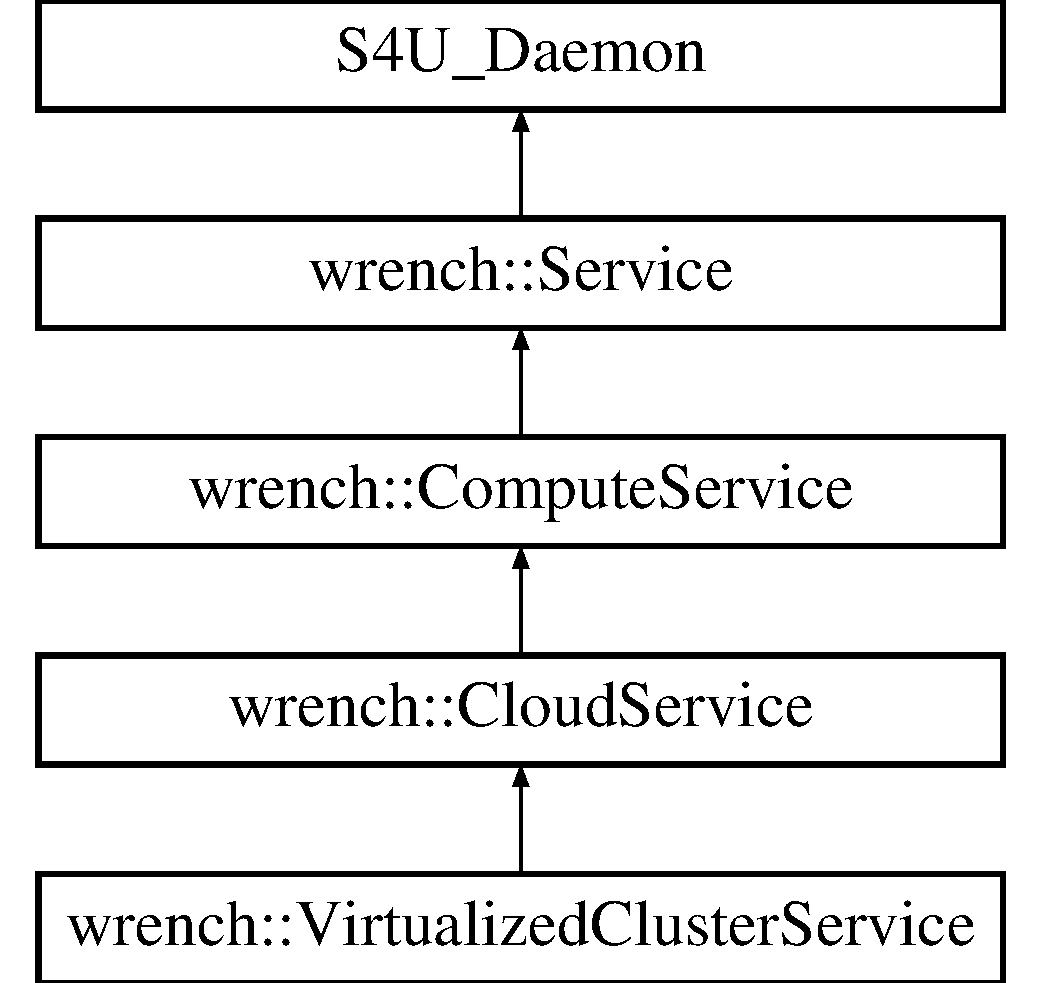
\includegraphics[height=5.000000cm]{classwrench_1_1_cloud_service}
\end{center}
\end{figure}
\subsection*{Public Member Functions}
\begin{DoxyCompactItemize}
\item 
\hyperlink{classwrench_1_1_cloud_service_a9f7f2d8bbbcaf2cd1c2cc881d11afec3}{Cloud\+Service} (const std\+::string \&hostname, std\+::vector$<$ std\+::string $>$ \&\hyperlink{classwrench_1_1_cloud_service_a8225cae457e491f3f3aad32653910ea0}{execution\+\_\+hosts}, double scratch\+\_\+space\+\_\+size, std\+::map$<$ std\+::string, std\+::string $>$ property\+\_\+list=\{\}, std\+::map$<$ std\+::string, std\+::string $>$ messagepayload\+\_\+list=\{\})
\begin{DoxyCompactList}\small\item\em Constructor. \end{DoxyCompactList}\end{DoxyCompactItemize}
\subsection*{Protected Attributes}
\begin{DoxyCompactItemize}
\item 
\mbox{\Hypertarget{classwrench_1_1_cloud_service_a56d772651ad005c9de543ca24327b9c6}\label{classwrench_1_1_cloud_service_a56d772651ad005c9de543ca24327b9c6}} 
std\+::map$<$ std\+::string, double $>$ \hyperlink{classwrench_1_1_cloud_service_a56d772651ad005c9de543ca24327b9c6}{cs\+\_\+available\+\_\+ram}
\begin{DoxyCompactList}\small\item\em Map of available R\+AM at hosts. \end{DoxyCompactList}\item 
\mbox{\Hypertarget{classwrench_1_1_cloud_service_a8225cae457e491f3f3aad32653910ea0}\label{classwrench_1_1_cloud_service_a8225cae457e491f3f3aad32653910ea0}} 
std\+::vector$<$ std\+::string $>$ \hyperlink{classwrench_1_1_cloud_service_a8225cae457e491f3f3aad32653910ea0}{execution\+\_\+hosts}
\begin{DoxyCompactList}\small\item\em List of execution host names. \end{DoxyCompactList}\item 
\mbox{\Hypertarget{classwrench_1_1_cloud_service_afda7fb1800d2d418e2a586925ffd4013}\label{classwrench_1_1_cloud_service_afda7fb1800d2d418e2a586925ffd4013}} 
std\+::map$<$ std\+::string, unsigned long $>$ \hyperlink{classwrench_1_1_cloud_service_afda7fb1800d2d418e2a586925ffd4013}{used\+\_\+cores\+\_\+per\+\_\+execution\+\_\+host}
\begin{DoxyCompactList}\small\item\em A map of the number of used cores (per VM) per execution host. \end{DoxyCompactList}\item 
\mbox{\Hypertarget{classwrench_1_1_cloud_service_a41782dd4332c11a992997562132f35e1}\label{classwrench_1_1_cloud_service_a41782dd4332c11a992997562132f35e1}} 
std\+::map$<$ std\+::string, std\+::tuple$<$ std\+::shared\+\_\+ptr$<$ S4\+U\+\_\+\+Virtual\+Machine $>$, std\+::shared\+\_\+ptr$<$ \hyperlink{classwrench_1_1_compute_service}{Compute\+Service} $>$, unsigned long, unsigned long $>$ $>$ \hyperlink{classwrench_1_1_cloud_service_a41782dd4332c11a992997562132f35e1}{vm\+\_\+list}
\begin{DoxyCompactList}\small\item\em A map of V\+Ms described by the VM actor, the actual compute service, the total number of cores, and R\+AM size. \end{DoxyCompactList}\end{DoxyCompactItemize}
\subsection*{Additional Inherited Members}


\subsection{Detailed Description}
A cloud-\/based compute service that manages a set of physical hosts and controls access to their resources by (transparently) executing jobs in VM instances. 

\subsection{Constructor \& Destructor Documentation}
\mbox{\Hypertarget{classwrench_1_1_cloud_service_a9f7f2d8bbbcaf2cd1c2cc881d11afec3}\label{classwrench_1_1_cloud_service_a9f7f2d8bbbcaf2cd1c2cc881d11afec3}} 
\index{wrench\+::\+Cloud\+Service@{wrench\+::\+Cloud\+Service}!Cloud\+Service@{Cloud\+Service}}
\index{Cloud\+Service@{Cloud\+Service}!wrench\+::\+Cloud\+Service@{wrench\+::\+Cloud\+Service}}
\subsubsection{\texorpdfstring{Cloud\+Service()}{CloudService()}}
{\footnotesize\ttfamily wrench\+::\+Cloud\+Service\+::\+Cloud\+Service (\begin{DoxyParamCaption}\item[{const std\+::string \&}]{hostname,  }\item[{std\+::vector$<$ std\+::string $>$ \&}]{execution\+\_\+hosts,  }\item[{double}]{scratch\+\_\+space\+\_\+size,  }\item[{std\+::map$<$ std\+::string, std\+::string $>$}]{property\+\_\+list = {\ttfamily \{\}},  }\item[{std\+::map$<$ std\+::string, std\+::string $>$}]{messagepayload\+\_\+list = {\ttfamily \{\}} }\end{DoxyParamCaption})}



Constructor. 


\begin{DoxyParams}{Parameters}
{\em hostname} & the hostname on which to start the service \\
\hline
{\em execution\+\_\+hosts} & the list of the names of the hosts available for running virtual machines \\
\hline
{\em scratch\+\_\+space\+\_\+size} & the size for the scratch storage pace of the cloud service \\
\hline
{\em property\+\_\+list} & a property list (\{\} means \char`\"{}use all defaults\char`\"{}) \\
\hline
{\em messagepayload\+\_\+list} & a message payload list (\{\} means \char`\"{}use all defaults\char`\"{})\\
\hline
\end{DoxyParams}

\begin{DoxyExceptions}{Exceptions}
{\em std\+::runtime\+\_\+error} & \\
\hline
\end{DoxyExceptions}


The documentation for this class was generated from the following files\+:\begin{DoxyCompactItemize}
\item 
/\+Users/rafsilva/\+Documents/isi/workspace/wrench/wrench/include/wrench/services/compute/cloud/Cloud\+Service.\+h\item 
/\+Users/rafsilva/\+Documents/isi/workspace/wrench/wrench/src/wrench/services/compute/cloud/Cloud\+Service.\+cpp\end{DoxyCompactItemize}

\hypertarget{classwrench_1_1_cloud_service_message_payload}{}\section{wrench\+:\+:Cloud\+Service\+Message\+Payload Class Reference}
\label{classwrench_1_1_cloud_service_message_payload}\index{wrench\+::\+Cloud\+Service\+Message\+Payload@{wrench\+::\+Cloud\+Service\+Message\+Payload}}


Configurable message payloads for a \hyperlink{classwrench_1_1_cloud_service}{Cloud\+Service}.  




{\ttfamily \#include $<$Cloud\+Service\+Message\+Payload.\+h$>$}

Inheritance diagram for wrench\+:\+:Cloud\+Service\+Message\+Payload\+:\begin{figure}[H]
\begin{center}
\leavevmode
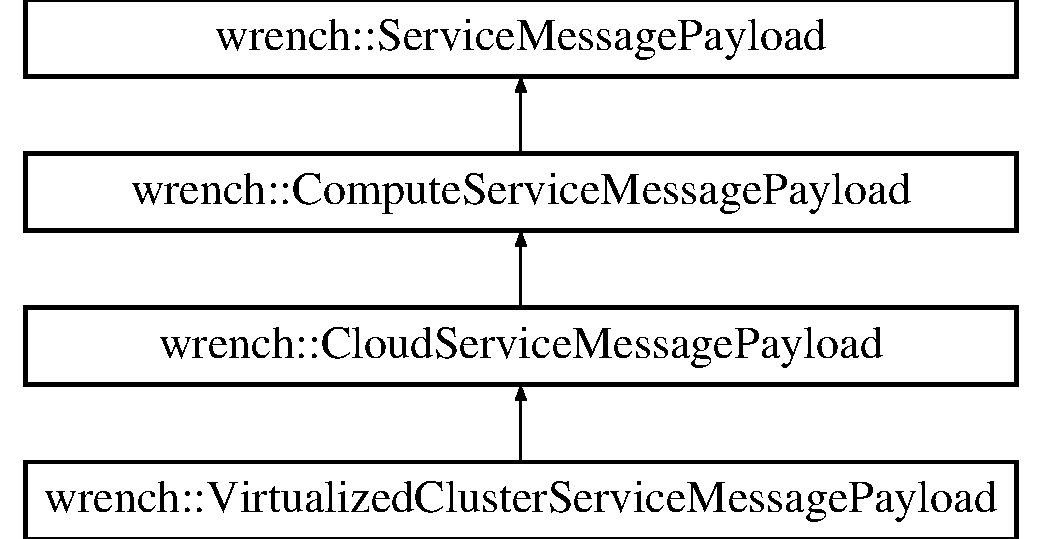
\includegraphics[height=4.000000cm]{classwrench_1_1_cloud_service_message_payload}
\end{center}
\end{figure}
\subsection*{Static Public Attributes}
\begin{DoxyCompactItemize}
\item 
\mbox{\Hypertarget{classwrench_1_1_cloud_service_message_payload_a4baff1046f125b8028edfc8b39ac3479}\label{classwrench_1_1_cloud_service_message_payload_a4baff1046f125b8028edfc8b39ac3479}} 
static const std\+::string \hyperlink{classwrench_1_1_cloud_service_message_payload_a4baff1046f125b8028edfc8b39ac3479}{C\+R\+E\+A\+T\+E\+\_\+\+V\+M\+\_\+\+A\+N\+S\+W\+E\+R\+\_\+\+M\+E\+S\+S\+A\+G\+E\+\_\+\+P\+A\+Y\+L\+O\+AD}
\begin{DoxyCompactList}\small\item\em The number of bytes in the control message sent by the service in answer to a VM creation request. \end{DoxyCompactList}\item 
\mbox{\Hypertarget{classwrench_1_1_cloud_service_message_payload_a02e27dcb5db011cc95718df537866eab}\label{classwrench_1_1_cloud_service_message_payload_a02e27dcb5db011cc95718df537866eab}} 
static const std\+::string \hyperlink{classwrench_1_1_cloud_service_message_payload_a02e27dcb5db011cc95718df537866eab}{C\+R\+E\+A\+T\+E\+\_\+\+V\+M\+\_\+\+R\+E\+Q\+U\+E\+S\+T\+\_\+\+M\+E\+S\+S\+A\+G\+E\+\_\+\+P\+A\+Y\+L\+O\+AD}
\begin{DoxyCompactList}\small\item\em The number of bytes in the control message sent to the service to request a VM creation. \end{DoxyCompactList}\item 
\mbox{\Hypertarget{classwrench_1_1_cloud_service_message_payload_a1a8446c3a946db300e5c19a13959bdd0}\label{classwrench_1_1_cloud_service_message_payload_a1a8446c3a946db300e5c19a13959bdd0}} 
static const std\+::string \hyperlink{classwrench_1_1_cloud_service_message_payload_a1a8446c3a946db300e5c19a13959bdd0}{G\+E\+T\+\_\+\+E\+X\+E\+C\+U\+T\+I\+O\+N\+\_\+\+H\+O\+S\+T\+S\+\_\+\+A\+N\+S\+W\+E\+R\+\_\+\+M\+E\+S\+S\+A\+G\+E\+\_\+\+P\+A\+Y\+L\+O\+AD}
\begin{DoxyCompactList}\small\item\em The number of bytes in the control message sent by the service in answer to a get execution hosts request. \end{DoxyCompactList}\item 
\mbox{\Hypertarget{classwrench_1_1_cloud_service_message_payload_a0c4ac7c65733155c7819d9c2b0528939}\label{classwrench_1_1_cloud_service_message_payload_a0c4ac7c65733155c7819d9c2b0528939}} 
static const std\+::string \hyperlink{classwrench_1_1_cloud_service_message_payload_a0c4ac7c65733155c7819d9c2b0528939}{G\+E\+T\+\_\+\+E\+X\+E\+C\+U\+T\+I\+O\+N\+\_\+\+H\+O\+S\+T\+S\+\_\+\+R\+E\+Q\+U\+E\+S\+T\+\_\+\+M\+E\+S\+S\+A\+G\+E\+\_\+\+P\+A\+Y\+L\+O\+AD}
\begin{DoxyCompactList}\small\item\em The number of bytes in the control message sent to the service to request a get execution hosts. \end{DoxyCompactList}\item 
\mbox{\Hypertarget{classwrench_1_1_cloud_service_message_payload_a79c5699f69b6fb6b2d0ae7a3ebcb3301}\label{classwrench_1_1_cloud_service_message_payload_a79c5699f69b6fb6b2d0ae7a3ebcb3301}} 
static const std\+::string \hyperlink{classwrench_1_1_cloud_service_message_payload_a79c5699f69b6fb6b2d0ae7a3ebcb3301}{R\+E\+S\+U\+M\+E\+\_\+\+V\+M\+\_\+\+A\+N\+S\+W\+E\+R\+\_\+\+M\+E\+S\+S\+A\+G\+E\+\_\+\+P\+A\+Y\+L\+O\+AD}
\begin{DoxyCompactList}\small\item\em The number of bytes in the control message sent by the service in answer to a VM resume request. \end{DoxyCompactList}\item 
\mbox{\Hypertarget{classwrench_1_1_cloud_service_message_payload_a18dbfc17cec5bf71e60a7b27e36024d7}\label{classwrench_1_1_cloud_service_message_payload_a18dbfc17cec5bf71e60a7b27e36024d7}} 
static const std\+::string \hyperlink{classwrench_1_1_cloud_service_message_payload_a18dbfc17cec5bf71e60a7b27e36024d7}{R\+E\+S\+U\+M\+E\+\_\+\+V\+M\+\_\+\+R\+E\+Q\+U\+E\+S\+T\+\_\+\+M\+E\+S\+S\+A\+G\+E\+\_\+\+P\+A\+Y\+L\+O\+AD}
\begin{DoxyCompactList}\small\item\em The number of bytes in the control message sent to the service to request a VM resume. \end{DoxyCompactList}\item 
\mbox{\Hypertarget{classwrench_1_1_cloud_service_message_payload_aa4788e4c91a26be675bfa29e827f529a}\label{classwrench_1_1_cloud_service_message_payload_aa4788e4c91a26be675bfa29e827f529a}} 
static const std\+::string \hyperlink{classwrench_1_1_cloud_service_message_payload_aa4788e4c91a26be675bfa29e827f529a}{S\+H\+U\+T\+D\+O\+W\+N\+\_\+\+V\+M\+\_\+\+A\+N\+S\+W\+E\+R\+\_\+\+M\+E\+S\+S\+A\+G\+E\+\_\+\+P\+A\+Y\+L\+O\+AD}
\begin{DoxyCompactList}\small\item\em The number of bytes in the control message sent by the service in answer to a VM shutdown request. \end{DoxyCompactList}\item 
\mbox{\Hypertarget{classwrench_1_1_cloud_service_message_payload_a2270e6fb3b1a4b583602bcb19877c3ee}\label{classwrench_1_1_cloud_service_message_payload_a2270e6fb3b1a4b583602bcb19877c3ee}} 
static const std\+::string \hyperlink{classwrench_1_1_cloud_service_message_payload_a2270e6fb3b1a4b583602bcb19877c3ee}{S\+H\+U\+T\+D\+O\+W\+N\+\_\+\+V\+M\+\_\+\+R\+E\+Q\+U\+E\+S\+T\+\_\+\+M\+E\+S\+S\+A\+G\+E\+\_\+\+P\+A\+Y\+L\+O\+AD}
\begin{DoxyCompactList}\small\item\em The number of bytes in the control message sent to the service to request a VM shutdown. \end{DoxyCompactList}\item 
\mbox{\Hypertarget{classwrench_1_1_cloud_service_message_payload_aa4bcd8c64fc1518561b9537158205a76}\label{classwrench_1_1_cloud_service_message_payload_aa4bcd8c64fc1518561b9537158205a76}} 
static const std\+::string \hyperlink{classwrench_1_1_cloud_service_message_payload_aa4bcd8c64fc1518561b9537158205a76}{S\+T\+A\+R\+T\+\_\+\+V\+M\+\_\+\+A\+N\+S\+W\+E\+R\+\_\+\+M\+E\+S\+S\+A\+G\+E\+\_\+\+P\+A\+Y\+L\+O\+AD}
\begin{DoxyCompactList}\small\item\em The number of bytes in the control message sent by the service in answer to a VM start request. \end{DoxyCompactList}\item 
\mbox{\Hypertarget{classwrench_1_1_cloud_service_message_payload_ac7663bdc3b3a6baf5a994d606e80c1cc}\label{classwrench_1_1_cloud_service_message_payload_ac7663bdc3b3a6baf5a994d606e80c1cc}} 
static const std\+::string \hyperlink{classwrench_1_1_cloud_service_message_payload_ac7663bdc3b3a6baf5a994d606e80c1cc}{S\+T\+A\+R\+T\+\_\+\+V\+M\+\_\+\+R\+E\+Q\+U\+E\+S\+T\+\_\+\+M\+E\+S\+S\+A\+G\+E\+\_\+\+P\+A\+Y\+L\+O\+AD}
\begin{DoxyCompactList}\small\item\em The number of bytes in the control message sent to the service to request a VM start. \end{DoxyCompactList}\item 
\mbox{\Hypertarget{classwrench_1_1_cloud_service_message_payload_ac31b4af8992603feaf301ba46f82a44b}\label{classwrench_1_1_cloud_service_message_payload_ac31b4af8992603feaf301ba46f82a44b}} 
static const std\+::string \hyperlink{classwrench_1_1_cloud_service_message_payload_ac31b4af8992603feaf301ba46f82a44b}{S\+U\+S\+P\+E\+N\+D\+\_\+\+V\+M\+\_\+\+A\+N\+S\+W\+E\+R\+\_\+\+M\+E\+S\+S\+A\+G\+E\+\_\+\+P\+A\+Y\+L\+O\+AD}
\begin{DoxyCompactList}\small\item\em The number of bytes in the control message sent by the service in answer to a VM suspend request. \end{DoxyCompactList}\item 
\mbox{\Hypertarget{classwrench_1_1_cloud_service_message_payload_a8eb571b25e35581f6e08126bdd0e0799}\label{classwrench_1_1_cloud_service_message_payload_a8eb571b25e35581f6e08126bdd0e0799}} 
static const std\+::string \hyperlink{classwrench_1_1_cloud_service_message_payload_a8eb571b25e35581f6e08126bdd0e0799}{S\+U\+S\+P\+E\+N\+D\+\_\+\+V\+M\+\_\+\+R\+E\+Q\+U\+E\+S\+T\+\_\+\+M\+E\+S\+S\+A\+G\+E\+\_\+\+P\+A\+Y\+L\+O\+AD}
\begin{DoxyCompactList}\small\item\em The number of bytes in the control message sent to the service to request a VM suspend. \end{DoxyCompactList}\end{DoxyCompactItemize}


\subsection{Detailed Description}
Configurable message payloads for a \hyperlink{classwrench_1_1_cloud_service}{Cloud\+Service}. 

The documentation for this class was generated from the following file\+:\begin{DoxyCompactItemize}
\item 
/\+Users/rafsilva/\+Documents/isi/workspace/wrench/wrench/include/wrench/services/compute/cloud/Cloud\+Service\+Message\+Payload.\+h\end{DoxyCompactItemize}

\hypertarget{classwrench_1_1_cloud_service_property}{}\section{wrench\+:\+:Cloud\+Service\+Property Class Reference}
\label{classwrench_1_1_cloud_service_property}\index{wrench\+::\+Cloud\+Service\+Property@{wrench\+::\+Cloud\+Service\+Property}}


Configurable properties for a \hyperlink{classwrench_1_1_cloud_service}{Cloud\+Service}.  




{\ttfamily \#include $<$Cloud\+Service\+Property.\+h$>$}

Inheritance diagram for wrench\+:\+:Cloud\+Service\+Property\+:\begin{figure}[H]
\begin{center}
\leavevmode
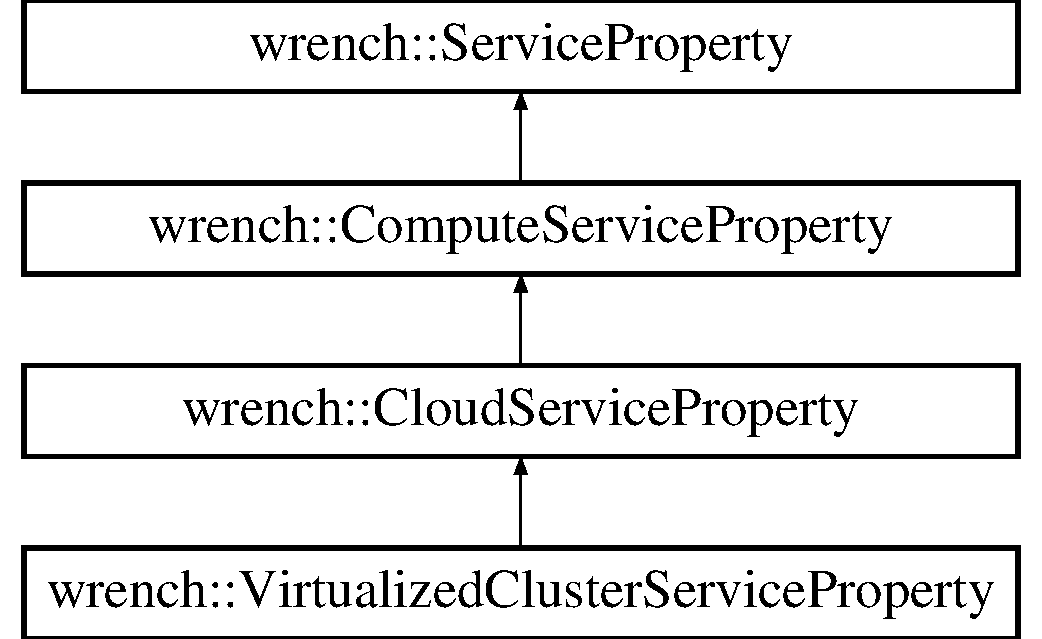
\includegraphics[height=4.000000cm]{classwrench_1_1_cloud_service_property}
\end{center}
\end{figure}
\subsection*{Static Public Attributes}
\begin{DoxyCompactItemize}
\item 
\mbox{\Hypertarget{classwrench_1_1_cloud_service_property_a7e2fddc7f539dedff89fb41635a5b200}\label{classwrench_1_1_cloud_service_property_a7e2fddc7f539dedff89fb41635a5b200}} 
static const std\+::string \hyperlink{classwrench_1_1_cloud_service_property_a7e2fddc7f539dedff89fb41635a5b200}{V\+M\+\_\+\+B\+O\+O\+T\+\_\+\+O\+V\+E\+R\+H\+E\+A\+D\+\_\+\+I\+N\+\_\+\+S\+E\+C\+O\+N\+DS}
\begin{DoxyCompactList}\small\item\em The overhead, in seconds, to boot a VM. \end{DoxyCompactList}\end{DoxyCompactItemize}


\subsection{Detailed Description}
Configurable properties for a \hyperlink{classwrench_1_1_cloud_service}{Cloud\+Service}. 

The documentation for this class was generated from the following file\+:\begin{DoxyCompactItemize}
\item 
/\+Users/rafsilva/\+Documents/isi/workspace/wrench/wrench/include/wrench/services/compute/cloud/Cloud\+Service\+Property.\+h\end{DoxyCompactItemize}

\hypertarget{classwrench_1_1_compute_service}{}\section{wrench\+:\+:Compute\+Service Class Reference}
\label{classwrench_1_1_compute_service}\index{wrench\+::\+Compute\+Service@{wrench\+::\+Compute\+Service}}


The compute service base class.  




{\ttfamily \#include $<$Compute\+Service.\+h$>$}

Inheritance diagram for wrench\+:\+:Compute\+Service\+:\begin{figure}[H]
\begin{center}
\leavevmode
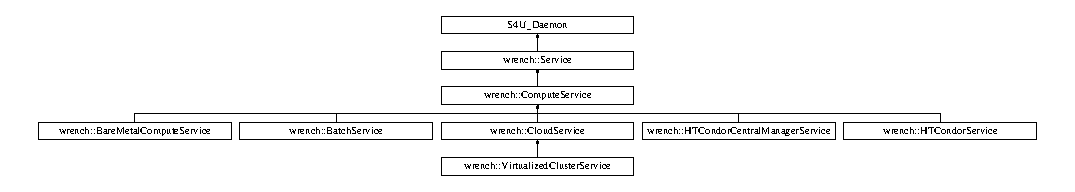
\includegraphics[height=2.137404cm]{classwrench_1_1_compute_service}
\end{center}
\end{figure}
\subsection*{Public Member Functions}
\begin{DoxyCompactItemize}
\item 
\hyperlink{classwrench_1_1_compute_service_abccb305cb121b093931392c937aa86e2}{Compute\+Service} (const std\+::string \&\hyperlink{classwrench_1_1_s4_u___daemon_a52bc0b9a6cd248310749dac086819f00}{hostname}, std\+::string service\+\_\+name, std\+::string mailbox\+\_\+name\+\_\+prefix, double scratch\+\_\+space\+\_\+size)
\begin{DoxyCompactList}\small\item\em Constructor. \end{DoxyCompactList}\item 
std\+::map$<$ std\+::string, double $>$ \hyperlink{classwrench_1_1_compute_service_a72c2608b82692ad73888d9b9f7c6bd0c}{get\+Core\+Flop\+Rate} ()
\begin{DoxyCompactList}\small\item\em Get the per-\/core flop rate of the compute service\textquotesingle{}s hosts. \end{DoxyCompactList}\item 
double \hyperlink{classwrench_1_1_compute_service_ac3662628f589ffe44e17921e60971fd6}{get\+Free\+Scratch\+Space\+Size} ()
\begin{DoxyCompactList}\small\item\em Get the free space on the compute service\textquotesingle{}s scratch storage space. \end{DoxyCompactList}\item 
std\+::map$<$ std\+::string, double $>$ \hyperlink{classwrench_1_1_compute_service_a113d9698fc83cefd78121e279b99b51e}{get\+Memory\+Capacity} ()
\begin{DoxyCompactList}\small\item\em Get the R\+AM capacities for each of the compute service\textquotesingle{}s hosts. \end{DoxyCompactList}\item 
std\+::map$<$ std\+::string, unsigned long $>$ \hyperlink{classwrench_1_1_compute_service_a0d88426f33110e811771f73f39c6458a}{get\+Num\+Cores} ()
\begin{DoxyCompactList}\small\item\em Get core counts for each of the compute service\textquotesingle{}s host. \end{DoxyCompactList}\item 
unsigned long \hyperlink{classwrench_1_1_compute_service_a1b576a22529bd638e6998f0513a44b36}{get\+Num\+Hosts} ()
\begin{DoxyCompactList}\small\item\em Get the number of hosts that the compute service manages. \end{DoxyCompactList}\item 
std\+::map$<$ std\+::string, unsigned long $>$ \hyperlink{classwrench_1_1_compute_service_a7d717171627835491772e589c4e6101f}{get\+Num\+Idle\+Cores} ()
\begin{DoxyCompactList}\small\item\em Get idle core counts for each of the compute service\textquotesingle{}s host. \end{DoxyCompactList}\item 
unsigned long \hyperlink{classwrench_1_1_compute_service_a5d2e4bca8b531521561f167769186f56}{get\+Total\+Num\+Cores} ()
\begin{DoxyCompactList}\small\item\em Get the total core counts for all hosts of the compute service. \end{DoxyCompactList}\item 
unsigned long \hyperlink{classwrench_1_1_compute_service_a225719efa4cb6c3b910c20e8828cb789}{get\+Total\+Num\+Idle\+Cores} ()
\begin{DoxyCompactList}\small\item\em Get the total idle core counts for all hosts of the compute service. \end{DoxyCompactList}\item 
double \hyperlink{classwrench_1_1_compute_service_ae0a8acd4a82063250799e313f1d520d1}{get\+Total\+Scratch\+Space\+Size} ()
\begin{DoxyCompactList}\small\item\em Get the total capacity of the compute service\textquotesingle{}s scratch storage space. \end{DoxyCompactList}\item 
double \hyperlink{classwrench_1_1_compute_service_a244e08a35ea94061acc1396f9447bb0c}{get\+T\+TL} ()
\begin{DoxyCompactList}\small\item\em Get the time-\/to-\/live of the compute service. \end{DoxyCompactList}\item 
bool \hyperlink{classwrench_1_1_compute_service_a07b64249656b26fef280c1f9db823acf}{has\+Scratch} ()
\begin{DoxyCompactList}\small\item\em Checks if the compute service has a scratch space. \end{DoxyCompactList}\item 
\mbox{\Hypertarget{classwrench_1_1_compute_service_a289d4a0c5254772575340095b73cf7d4}\label{classwrench_1_1_compute_service_a289d4a0c5254772575340095b73cf7d4}} 
void \hyperlink{classwrench_1_1_compute_service_a289d4a0c5254772575340095b73cf7d4}{stop} () override
\begin{DoxyCompactList}\small\item\em Stop the compute service -\/ must be called by the \hyperlink{classwrench_1_1_compute_service_a289d4a0c5254772575340095b73cf7d4}{stop()} method of derived classes. \end{DoxyCompactList}\item 
void \hyperlink{classwrench_1_1_compute_service_abc9e51234c29965341727f07b446ff0c}{submit\+Job} (\hyperlink{classwrench_1_1_workflow_job}{Workflow\+Job} $\ast$job, std\+::map$<$ std\+::string, std\+::string $>$=\{\})
\begin{DoxyCompactList}\small\item\em Submit a job to the compute service. \end{DoxyCompactList}\item 
\mbox{\Hypertarget{classwrench_1_1_compute_service_a96d4857d6e9ec654d8d48b046a87924d}\label{classwrench_1_1_compute_service_a96d4857d6e9ec654d8d48b046a87924d}} 
virtual void {\bfseries submit\+Pilot\+Job} (\hyperlink{classwrench_1_1_pilot_job}{Pilot\+Job} $\ast$job, std\+::map$<$ std\+::string, std\+::string $>$ \&service\+\_\+specific\+\_\+arguments)=0
\item 
\mbox{\Hypertarget{classwrench_1_1_compute_service_a3b6015d44a0410b957346ccbc29f715d}\label{classwrench_1_1_compute_service_a3b6015d44a0410b957346ccbc29f715d}} 
virtual void {\bfseries submit\+Standard\+Job} (\hyperlink{classwrench_1_1_standard_job}{Standard\+Job} $\ast$job, std\+::map$<$ std\+::string, std\+::string $>$ \&service\+\_\+specific\+\_\+arguments)=0
\item 
bool \hyperlink{classwrench_1_1_compute_service_acd8cd30b0c6a7f23be2a16e9c8910822}{supports\+Pilot\+Jobs} ()
\begin{DoxyCompactList}\small\item\em Get whether the compute service supports pilot jobs or not. \end{DoxyCompactList}\item 
bool \hyperlink{classwrench_1_1_compute_service_a0f15f4038c447b0f580b9d2a7bf0cd22}{supports\+Standard\+Jobs} ()
\begin{DoxyCompactList}\small\item\em Get whether the compute service supports standard jobs or not. \end{DoxyCompactList}\item 
void \hyperlink{classwrench_1_1_compute_service_aba97c346fb8f171f17ec09681be37d7f}{terminate\+Job} (\hyperlink{classwrench_1_1_workflow_job}{Workflow\+Job} $\ast$job)
\begin{DoxyCompactList}\small\item\em Terminate a previously-\/submitted job (which may or may not be running yet) \end{DoxyCompactList}\item 
\mbox{\Hypertarget{classwrench_1_1_compute_service_aba3fad85c3f62b9764fc5a05d4d0edd0}\label{classwrench_1_1_compute_service_aba3fad85c3f62b9764fc5a05d4d0edd0}} 
virtual void {\bfseries terminate\+Pilot\+Job} (\hyperlink{classwrench_1_1_pilot_job}{Pilot\+Job} $\ast$job)=0
\item 
\mbox{\Hypertarget{classwrench_1_1_compute_service_aa648a19b246d650827924d0e829dd2b6}\label{classwrench_1_1_compute_service_aa648a19b246d650827924d0e829dd2b6}} 
virtual void {\bfseries terminate\+Standard\+Job} (\hyperlink{classwrench_1_1_standard_job}{Standard\+Job} $\ast$job)=0
\end{DoxyCompactItemize}
\subsection*{Static Public Attributes}
\begin{DoxyCompactItemize}
\item 
\mbox{\Hypertarget{classwrench_1_1_compute_service_a1160f521623440ad4e0e0823e08a7d22}\label{classwrench_1_1_compute_service_a1160f521623440ad4e0e0823e08a7d22}} 
static constexpr unsigned long \hyperlink{classwrench_1_1_compute_service_a1160f521623440ad4e0e0823e08a7d22}{A\+L\+L\+\_\+\+C\+O\+R\+ES} = U\+L\+O\+N\+G\+\_\+\+M\+AX
\begin{DoxyCompactList}\small\item\em A convenient constant to mean \char`\"{}use all cores of a physical host\char`\"{} whenever a number of cores is needed when instantiating compute services. \end{DoxyCompactList}\item 
\mbox{\Hypertarget{classwrench_1_1_compute_service_abc4fe0bad59f544b4b34d0e7d4012d44}\label{classwrench_1_1_compute_service_abc4fe0bad59f544b4b34d0e7d4012d44}} 
static constexpr double \hyperlink{classwrench_1_1_compute_service_abc4fe0bad59f544b4b34d0e7d4012d44}{A\+L\+L\+\_\+\+R\+AM} = D\+B\+L\+\_\+\+M\+AX
\begin{DoxyCompactList}\small\item\em A convenient constant to mean \char`\"{}use all ram of a physical host\char`\"{} whenever a ram capacity is needed when instantiating compute services. \end{DoxyCompactList}\item 
\mbox{\Hypertarget{classwrench_1_1_compute_service_a022e9408f53191b4102e2ce00487799c}\label{classwrench_1_1_compute_service_a022e9408f53191b4102e2ce00487799c}} 
static \hyperlink{classwrench_1_1_storage_service}{Storage\+Service} $\ast$ \hyperlink{classwrench_1_1_compute_service_a022e9408f53191b4102e2ce00487799c}{S\+C\+R\+A\+T\+CH} = (\hyperlink{classwrench_1_1_storage_service}{Storage\+Service} $\ast$) U\+L\+O\+N\+G\+\_\+\+M\+AX
\begin{DoxyCompactList}\small\item\em A convenient constant to mean \char`\"{}the scratch storage space\char`\"{} of a \hyperlink{classwrench_1_1_compute_service}{Compute\+Service}. This is used to move data to a \hyperlink{classwrench_1_1_compute_service}{Compute\+Service}\textquotesingle{}s scratch storage space. \end{DoxyCompactList}\end{DoxyCompactItemize}
\subsection*{Protected Member Functions}
\begin{DoxyCompactItemize}
\item 
\hyperlink{classwrench_1_1_compute_service_afa84f3dd13d7fac9632ded22db2d8c4f}{Compute\+Service} (const std\+::string \&\hyperlink{classwrench_1_1_s4_u___daemon_a52bc0b9a6cd248310749dac086819f00}{hostname}, std\+::string service\+\_\+name, std\+::string mailbox\+\_\+name\+\_\+prefix, \hyperlink{classwrench_1_1_storage_service}{Storage\+Service} $\ast$scratch\+\_\+space)
\begin{DoxyCompactList}\small\item\em Constructor. \end{DoxyCompactList}\item 
\hyperlink{classwrench_1_1_storage_service}{Storage\+Service} $\ast$ \hyperlink{classwrench_1_1_compute_service_a751da474fe424957a614116cef6a5e13}{get\+Scratch} ()
\begin{DoxyCompactList}\small\item\em Get the compute service\textquotesingle{}s scratch storage space. \end{DoxyCompactList}\item 
std\+::shared\+\_\+ptr$<$ \hyperlink{classwrench_1_1_storage_service}{Storage\+Service} $>$ \hyperlink{classwrench_1_1_compute_service_a6532846cd02094b6095341d37d5b2bf7}{get\+Scratch\+Shared\+Ptr} ()
\begin{DoxyCompactList}\small\item\em Get a shared pointer to the compute service\textquotesingle{}s scratch storage space. \end{DoxyCompactList}\end{DoxyCompactItemize}
\subsection*{Protected Attributes}
\begin{DoxyCompactItemize}
\item 
\mbox{\Hypertarget{classwrench_1_1_compute_service_a41fa63f7200275c18f3bcb0dda9099a5}\label{classwrench_1_1_compute_service_a41fa63f7200275c18f3bcb0dda9099a5}} 
\hyperlink{classwrench_1_1_storage_service}{Storage\+Service} $\ast$ \hyperlink{classwrench_1_1_compute_service_a41fa63f7200275c18f3bcb0dda9099a5}{scratch\+\_\+space\+\_\+storage\+\_\+service}
\begin{DoxyCompactList}\small\item\em A scratch storage service associated to the compute service. \end{DoxyCompactList}\item 
\mbox{\Hypertarget{classwrench_1_1_compute_service_a851cc870ccd1b6c9243fb83cbb34be71}\label{classwrench_1_1_compute_service_a851cc870ccd1b6c9243fb83cbb34be71}} 
std\+::shared\+\_\+ptr$<$ \hyperlink{classwrench_1_1_storage_service}{Storage\+Service} $>$ {\bfseries scratch\+\_\+space\+\_\+storage\+\_\+service\+\_\+shared\+\_\+ptr}
\end{DoxyCompactItemize}
\subsection*{Additional Inherited Members}


\subsection{Detailed Description}
The compute service base class. 

\subsection{Constructor \& Destructor Documentation}
\mbox{\Hypertarget{classwrench_1_1_compute_service_abccb305cb121b093931392c937aa86e2}\label{classwrench_1_1_compute_service_abccb305cb121b093931392c937aa86e2}} 
\index{wrench\+::\+Compute\+Service@{wrench\+::\+Compute\+Service}!Compute\+Service@{Compute\+Service}}
\index{Compute\+Service@{Compute\+Service}!wrench\+::\+Compute\+Service@{wrench\+::\+Compute\+Service}}
\subsubsection{\texorpdfstring{Compute\+Service()}{ComputeService()}\hspace{0.1cm}{\footnotesize\ttfamily [1/2]}}
{\footnotesize\ttfamily wrench\+::\+Compute\+Service\+::\+Compute\+Service (\begin{DoxyParamCaption}\item[{const std\+::string \&}]{hostname,  }\item[{std\+::string}]{service\+\_\+name,  }\item[{std\+::string}]{mailbox\+\_\+name\+\_\+prefix,  }\item[{double}]{scratch\+\_\+space\+\_\+size }\end{DoxyParamCaption})}



Constructor. 


\begin{DoxyParams}{Parameters}
{\em hostname} & the name of the host on which the compute service runs \\
\hline
{\em service\+\_\+name} & the name of the compute service \\
\hline
{\em mailbox\+\_\+name\+\_\+prefix} & the mailbox name prefix \\
\hline
{\em scratch\+\_\+space\+\_\+size} & the size for the scratch storage space of the compute service (0 if none) \\
\hline
\end{DoxyParams}
\mbox{\Hypertarget{classwrench_1_1_compute_service_afa84f3dd13d7fac9632ded22db2d8c4f}\label{classwrench_1_1_compute_service_afa84f3dd13d7fac9632ded22db2d8c4f}} 
\index{wrench\+::\+Compute\+Service@{wrench\+::\+Compute\+Service}!Compute\+Service@{Compute\+Service}}
\index{Compute\+Service@{Compute\+Service}!wrench\+::\+Compute\+Service@{wrench\+::\+Compute\+Service}}
\subsubsection{\texorpdfstring{Compute\+Service()}{ComputeService()}\hspace{0.1cm}{\footnotesize\ttfamily [2/2]}}
{\footnotesize\ttfamily wrench\+::\+Compute\+Service\+::\+Compute\+Service (\begin{DoxyParamCaption}\item[{const std\+::string \&}]{hostname,  }\item[{std\+::string}]{service\+\_\+name,  }\item[{std\+::string}]{mailbox\+\_\+name\+\_\+prefix,  }\item[{\hyperlink{classwrench_1_1_storage_service}{Storage\+Service} $\ast$}]{scratch\+\_\+space }\end{DoxyParamCaption})\hspace{0.3cm}{\ttfamily [protected]}}



Constructor. 


\begin{DoxyParams}{Parameters}
{\em hostname} & the name of the host on which the compute service runs \\
\hline
{\em service\+\_\+name} & the name of the compute service \\
\hline
{\em mailbox\+\_\+name\+\_\+prefix} & the mailbox name prefix \\
\hline
{\em scratch\+\_\+space} & scratch storage space of the compute service (nullptr if none) \\
\hline
\end{DoxyParams}


\subsection{Member Function Documentation}
\mbox{\Hypertarget{classwrench_1_1_compute_service_a72c2608b82692ad73888d9b9f7c6bd0c}\label{classwrench_1_1_compute_service_a72c2608b82692ad73888d9b9f7c6bd0c}} 
\index{wrench\+::\+Compute\+Service@{wrench\+::\+Compute\+Service}!get\+Core\+Flop\+Rate@{get\+Core\+Flop\+Rate}}
\index{get\+Core\+Flop\+Rate@{get\+Core\+Flop\+Rate}!wrench\+::\+Compute\+Service@{wrench\+::\+Compute\+Service}}
\subsubsection{\texorpdfstring{get\+Core\+Flop\+Rate()}{getCoreFlopRate()}}
{\footnotesize\ttfamily std\+::map$<$ std\+::string, double $>$ wrench\+::\+Compute\+Service\+::get\+Core\+Flop\+Rate (\begin{DoxyParamCaption}{ }\end{DoxyParamCaption})}



Get the per-\/core flop rate of the compute service\textquotesingle{}s hosts. 

\begin{DoxyReturn}{Returns}
a list of flop rates in flop/sec
\end{DoxyReturn}

\begin{DoxyExceptions}{Exceptions}
{\em std\+::runtime\+\_\+error} & \\
\hline
\end{DoxyExceptions}
\mbox{\Hypertarget{classwrench_1_1_compute_service_ac3662628f589ffe44e17921e60971fd6}\label{classwrench_1_1_compute_service_ac3662628f589ffe44e17921e60971fd6}} 
\index{wrench\+::\+Compute\+Service@{wrench\+::\+Compute\+Service}!get\+Free\+Scratch\+Space\+Size@{get\+Free\+Scratch\+Space\+Size}}
\index{get\+Free\+Scratch\+Space\+Size@{get\+Free\+Scratch\+Space\+Size}!wrench\+::\+Compute\+Service@{wrench\+::\+Compute\+Service}}
\subsubsection{\texorpdfstring{get\+Free\+Scratch\+Space\+Size()}{getFreeScratchSpaceSize()}}
{\footnotesize\ttfamily double wrench\+::\+Compute\+Service\+::get\+Free\+Scratch\+Space\+Size (\begin{DoxyParamCaption}{ }\end{DoxyParamCaption})}



Get the free space on the compute service\textquotesingle{}s scratch storage space. 

\begin{DoxyReturn}{Returns}
a size (in bytes) 
\end{DoxyReturn}
\mbox{\Hypertarget{classwrench_1_1_compute_service_a113d9698fc83cefd78121e279b99b51e}\label{classwrench_1_1_compute_service_a113d9698fc83cefd78121e279b99b51e}} 
\index{wrench\+::\+Compute\+Service@{wrench\+::\+Compute\+Service}!get\+Memory\+Capacity@{get\+Memory\+Capacity}}
\index{get\+Memory\+Capacity@{get\+Memory\+Capacity}!wrench\+::\+Compute\+Service@{wrench\+::\+Compute\+Service}}
\subsubsection{\texorpdfstring{get\+Memory\+Capacity()}{getMemoryCapacity()}}
{\footnotesize\ttfamily std\+::map$<$ std\+::string, double $>$ wrench\+::\+Compute\+Service\+::get\+Memory\+Capacity (\begin{DoxyParamCaption}{ }\end{DoxyParamCaption})}



Get the R\+AM capacities for each of the compute service\textquotesingle{}s hosts. 

\begin{DoxyReturn}{Returns}
a map of R\+AM capacities, indexed by hostname
\end{DoxyReturn}

\begin{DoxyExceptions}{Exceptions}
{\em std\+::runtime\+\_\+error} & \\
\hline
\end{DoxyExceptions}
\mbox{\Hypertarget{classwrench_1_1_compute_service_a0d88426f33110e811771f73f39c6458a}\label{classwrench_1_1_compute_service_a0d88426f33110e811771f73f39c6458a}} 
\index{wrench\+::\+Compute\+Service@{wrench\+::\+Compute\+Service}!get\+Num\+Cores@{get\+Num\+Cores}}
\index{get\+Num\+Cores@{get\+Num\+Cores}!wrench\+::\+Compute\+Service@{wrench\+::\+Compute\+Service}}
\subsubsection{\texorpdfstring{get\+Num\+Cores()}{getNumCores()}}
{\footnotesize\ttfamily std\+::map$<$ std\+::string, unsigned long $>$ wrench\+::\+Compute\+Service\+::get\+Num\+Cores (\begin{DoxyParamCaption}{ }\end{DoxyParamCaption})}



Get core counts for each of the compute service\textquotesingle{}s host. 

\begin{DoxyReturn}{Returns}
a map of core counts, indexed by hostnames
\end{DoxyReturn}

\begin{DoxyExceptions}{Exceptions}
{\em \hyperlink{classwrench_1_1_workflow_execution_exception}{Workflow\+Execution\+Exception}} & \\
\hline
{\em std\+::runtime\+\_\+error} & \\
\hline
\end{DoxyExceptions}
\mbox{\Hypertarget{classwrench_1_1_compute_service_a1b576a22529bd638e6998f0513a44b36}\label{classwrench_1_1_compute_service_a1b576a22529bd638e6998f0513a44b36}} 
\index{wrench\+::\+Compute\+Service@{wrench\+::\+Compute\+Service}!get\+Num\+Hosts@{get\+Num\+Hosts}}
\index{get\+Num\+Hosts@{get\+Num\+Hosts}!wrench\+::\+Compute\+Service@{wrench\+::\+Compute\+Service}}
\subsubsection{\texorpdfstring{get\+Num\+Hosts()}{getNumHosts()}}
{\footnotesize\ttfamily unsigned long wrench\+::\+Compute\+Service\+::get\+Num\+Hosts (\begin{DoxyParamCaption}{ }\end{DoxyParamCaption})}



Get the number of hosts that the compute service manages. 

\begin{DoxyReturn}{Returns}
the host count
\end{DoxyReturn}

\begin{DoxyExceptions}{Exceptions}
{\em \hyperlink{classwrench_1_1_workflow_execution_exception}{Workflow\+Execution\+Exception}} & \\
\hline
{\em std\+::runtime\+\_\+error} & \\
\hline
\end{DoxyExceptions}
\mbox{\Hypertarget{classwrench_1_1_compute_service_a7d717171627835491772e589c4e6101f}\label{classwrench_1_1_compute_service_a7d717171627835491772e589c4e6101f}} 
\index{wrench\+::\+Compute\+Service@{wrench\+::\+Compute\+Service}!get\+Num\+Idle\+Cores@{get\+Num\+Idle\+Cores}}
\index{get\+Num\+Idle\+Cores@{get\+Num\+Idle\+Cores}!wrench\+::\+Compute\+Service@{wrench\+::\+Compute\+Service}}
\subsubsection{\texorpdfstring{get\+Num\+Idle\+Cores()}{getNumIdleCores()}}
{\footnotesize\ttfamily std\+::map$<$ std\+::string, unsigned long $>$ wrench\+::\+Compute\+Service\+::get\+Num\+Idle\+Cores (\begin{DoxyParamCaption}{ }\end{DoxyParamCaption})}



Get idle core counts for each of the compute service\textquotesingle{}s host. 

\begin{DoxyReturn}{Returns}
the idle core counts (could be empty)
\end{DoxyReturn}

\begin{DoxyExceptions}{Exceptions}
{\em \hyperlink{classwrench_1_1_workflow_execution_exception}{Workflow\+Execution\+Exception}} & \\
\hline
{\em std\+::runtime\+\_\+error} & \\
\hline
\end{DoxyExceptions}
\mbox{\Hypertarget{classwrench_1_1_compute_service_a751da474fe424957a614116cef6a5e13}\label{classwrench_1_1_compute_service_a751da474fe424957a614116cef6a5e13}} 
\index{wrench\+::\+Compute\+Service@{wrench\+::\+Compute\+Service}!get\+Scratch@{get\+Scratch}}
\index{get\+Scratch@{get\+Scratch}!wrench\+::\+Compute\+Service@{wrench\+::\+Compute\+Service}}
\subsubsection{\texorpdfstring{get\+Scratch()}{getScratch()}}
{\footnotesize\ttfamily \hyperlink{classwrench_1_1_storage_service}{Storage\+Service} $\ast$ wrench\+::\+Compute\+Service\+::get\+Scratch (\begin{DoxyParamCaption}{ }\end{DoxyParamCaption})\hspace{0.3cm}{\ttfamily [protected]}}



Get the compute service\textquotesingle{}s scratch storage space. 

\begin{DoxyReturn}{Returns}
a pointer to the shared scratch space 
\end{DoxyReturn}
\mbox{\Hypertarget{classwrench_1_1_compute_service_a6532846cd02094b6095341d37d5b2bf7}\label{classwrench_1_1_compute_service_a6532846cd02094b6095341d37d5b2bf7}} 
\index{wrench\+::\+Compute\+Service@{wrench\+::\+Compute\+Service}!get\+Scratch\+Shared\+Ptr@{get\+Scratch\+Shared\+Ptr}}
\index{get\+Scratch\+Shared\+Ptr@{get\+Scratch\+Shared\+Ptr}!wrench\+::\+Compute\+Service@{wrench\+::\+Compute\+Service}}
\subsubsection{\texorpdfstring{get\+Scratch\+Shared\+Ptr()}{getScratchSharedPtr()}}
{\footnotesize\ttfamily std\+::shared\+\_\+ptr$<$ \hyperlink{classwrench_1_1_storage_service}{Storage\+Service} $>$ wrench\+::\+Compute\+Service\+::get\+Scratch\+Shared\+Ptr (\begin{DoxyParamCaption}{ }\end{DoxyParamCaption})\hspace{0.3cm}{\ttfamily [protected]}}



Get a shared pointer to the compute service\textquotesingle{}s scratch storage space. 

\begin{DoxyReturn}{Returns}
a shared pointer to the shared scratch space 
\end{DoxyReturn}
\mbox{\Hypertarget{classwrench_1_1_compute_service_a5d2e4bca8b531521561f167769186f56}\label{classwrench_1_1_compute_service_a5d2e4bca8b531521561f167769186f56}} 
\index{wrench\+::\+Compute\+Service@{wrench\+::\+Compute\+Service}!get\+Total\+Num\+Cores@{get\+Total\+Num\+Cores}}
\index{get\+Total\+Num\+Cores@{get\+Total\+Num\+Cores}!wrench\+::\+Compute\+Service@{wrench\+::\+Compute\+Service}}
\subsubsection{\texorpdfstring{get\+Total\+Num\+Cores()}{getTotalNumCores()}}
{\footnotesize\ttfamily unsigned long wrench\+::\+Compute\+Service\+::get\+Total\+Num\+Cores (\begin{DoxyParamCaption}{ }\end{DoxyParamCaption})}



Get the total core counts for all hosts of the compute service. 

\begin{DoxyReturn}{Returns}
total core counts
\end{DoxyReturn}

\begin{DoxyExceptions}{Exceptions}
{\em \hyperlink{classwrench_1_1_workflow_execution_exception}{Workflow\+Execution\+Exception}} & \\
\hline
{\em std\+::runtime\+\_\+error} & \\
\hline
\end{DoxyExceptions}
\mbox{\Hypertarget{classwrench_1_1_compute_service_a225719efa4cb6c3b910c20e8828cb789}\label{classwrench_1_1_compute_service_a225719efa4cb6c3b910c20e8828cb789}} 
\index{wrench\+::\+Compute\+Service@{wrench\+::\+Compute\+Service}!get\+Total\+Num\+Idle\+Cores@{get\+Total\+Num\+Idle\+Cores}}
\index{get\+Total\+Num\+Idle\+Cores@{get\+Total\+Num\+Idle\+Cores}!wrench\+::\+Compute\+Service@{wrench\+::\+Compute\+Service}}
\subsubsection{\texorpdfstring{get\+Total\+Num\+Idle\+Cores()}{getTotalNumIdleCores()}}
{\footnotesize\ttfamily unsigned long wrench\+::\+Compute\+Service\+::get\+Total\+Num\+Idle\+Cores (\begin{DoxyParamCaption}{ }\end{DoxyParamCaption})}



Get the total idle core counts for all hosts of the compute service. 

\begin{DoxyReturn}{Returns}
total idle core counts
\end{DoxyReturn}

\begin{DoxyExceptions}{Exceptions}
{\em \hyperlink{classwrench_1_1_workflow_execution_exception}{Workflow\+Execution\+Exception}} & \\
\hline
{\em std\+::runtime\+\_\+error} & \\
\hline
\end{DoxyExceptions}
\mbox{\Hypertarget{classwrench_1_1_compute_service_ae0a8acd4a82063250799e313f1d520d1}\label{classwrench_1_1_compute_service_ae0a8acd4a82063250799e313f1d520d1}} 
\index{wrench\+::\+Compute\+Service@{wrench\+::\+Compute\+Service}!get\+Total\+Scratch\+Space\+Size@{get\+Total\+Scratch\+Space\+Size}}
\index{get\+Total\+Scratch\+Space\+Size@{get\+Total\+Scratch\+Space\+Size}!wrench\+::\+Compute\+Service@{wrench\+::\+Compute\+Service}}
\subsubsection{\texorpdfstring{get\+Total\+Scratch\+Space\+Size()}{getTotalScratchSpaceSize()}}
{\footnotesize\ttfamily double wrench\+::\+Compute\+Service\+::get\+Total\+Scratch\+Space\+Size (\begin{DoxyParamCaption}{ }\end{DoxyParamCaption})}



Get the total capacity of the compute service\textquotesingle{}s scratch storage space. 

\begin{DoxyReturn}{Returns}
a size (in bytes) 
\end{DoxyReturn}
\mbox{\Hypertarget{classwrench_1_1_compute_service_a244e08a35ea94061acc1396f9447bb0c}\label{classwrench_1_1_compute_service_a244e08a35ea94061acc1396f9447bb0c}} 
\index{wrench\+::\+Compute\+Service@{wrench\+::\+Compute\+Service}!get\+T\+TL@{get\+T\+TL}}
\index{get\+T\+TL@{get\+T\+TL}!wrench\+::\+Compute\+Service@{wrench\+::\+Compute\+Service}}
\subsubsection{\texorpdfstring{get\+T\+T\+L()}{getTTL()}}
{\footnotesize\ttfamily double wrench\+::\+Compute\+Service\+::get\+T\+TL (\begin{DoxyParamCaption}{ }\end{DoxyParamCaption})}



Get the time-\/to-\/live of the compute service. 

\begin{DoxyReturn}{Returns}
the ttl in seconds
\end{DoxyReturn}

\begin{DoxyExceptions}{Exceptions}
{\em std\+::runtime\+\_\+error} & \\
\hline
\end{DoxyExceptions}
\mbox{\Hypertarget{classwrench_1_1_compute_service_a07b64249656b26fef280c1f9db823acf}\label{classwrench_1_1_compute_service_a07b64249656b26fef280c1f9db823acf}} 
\index{wrench\+::\+Compute\+Service@{wrench\+::\+Compute\+Service}!has\+Scratch@{has\+Scratch}}
\index{has\+Scratch@{has\+Scratch}!wrench\+::\+Compute\+Service@{wrench\+::\+Compute\+Service}}
\subsubsection{\texorpdfstring{has\+Scratch()}{hasScratch()}}
{\footnotesize\ttfamily bool wrench\+::\+Compute\+Service\+::has\+Scratch (\begin{DoxyParamCaption}{ }\end{DoxyParamCaption})}



Checks if the compute service has a scratch space. 

\begin{DoxyReturn}{Returns}
true if the compute service has some scratch storage space, false otherwise 
\end{DoxyReturn}
\mbox{\Hypertarget{classwrench_1_1_compute_service_abc9e51234c29965341727f07b446ff0c}\label{classwrench_1_1_compute_service_abc9e51234c29965341727f07b446ff0c}} 
\index{wrench\+::\+Compute\+Service@{wrench\+::\+Compute\+Service}!submit\+Job@{submit\+Job}}
\index{submit\+Job@{submit\+Job}!wrench\+::\+Compute\+Service@{wrench\+::\+Compute\+Service}}
\subsubsection{\texorpdfstring{submit\+Job()}{submitJob()}}
{\footnotesize\ttfamily void wrench\+::\+Compute\+Service\+::submit\+Job (\begin{DoxyParamCaption}\item[{\hyperlink{classwrench_1_1_workflow_job}{Workflow\+Job} $\ast$}]{job,  }\item[{std\+::map$<$ std\+::string, std\+::string $>$}]{service\+\_\+specific\+\_\+args = {\ttfamily \{\}} }\end{DoxyParamCaption})}



Submit a job to the compute service. 


\begin{DoxyParams}{Parameters}
{\em job} & the job \\
\hline
{\em service\+\_\+specific\+\_\+args} & arguments specific to compute services when needed\+:
\begin{DoxyItemize}
\item to a \hyperlink{classwrench_1_1_bare_metal_compute_service}{Bare\+Metal\+Compute\+Service}\+: \{\}
\begin{DoxyItemize}
\item If no entry is provided for a task\+ID, the service will pick on which host and with how many cores to run the task
\item If a number of cores is provided (e.\+g., \{\char`\"{}task1\char`\"{}, \char`\"{}12\char`\"{}\}), the service will pick the host on which to run the task
\item If a hostname and a number of cores is provided (e.\+g., \{\char`\"{}task1\char`\"{}, \char`\"{}host1\+:12\char`\"{}\}, the service will run the task on that host with the specified number of cores
\end{DoxyItemize}
\item to a \hyperlink{classwrench_1_1_batch_service}{Batch\+Service}\+: \{\char`\"{}-\/t\char`\"{}\+:\char`\"{}$<$int$>$\char`\"{},\char`\"{}-\/\+N\char`\"{}\+:\char`\"{}$<$int$>$\char`\"{},\char`\"{}-\/c\char`\"{}\+:\char`\"{}$<$int$>$\char`\"{}\} (S\+L\+U\+R\+M-\/like)
\begin{DoxyItemize}
\item \char`\"{}-\/t\char`\"{}\+: number of requested job duration in minutes
\item \char`\"{}-\/\+N\char`\"{}\+: number of requested compute hosts
\item \char`\"{}-\/c\char`\"{}\+: number of requested cores per compute host
\end{DoxyItemize}
\item to a \hyperlink{classwrench_1_1_cloud_service}{Cloud\+Service}\+: \{\}
\end{DoxyItemize}\\
\hline
\end{DoxyParams}

\begin{DoxyExceptions}{Exceptions}
{\em \hyperlink{classwrench_1_1_workflow_execution_exception}{Workflow\+Execution\+Exception}} & \\
\hline
{\em std\+::invalid\+\_\+argument} & \\
\hline
{\em std\+::runtime\+\_\+error} & \\
\hline
\end{DoxyExceptions}
\mbox{\Hypertarget{classwrench_1_1_compute_service_acd8cd30b0c6a7f23be2a16e9c8910822}\label{classwrench_1_1_compute_service_acd8cd30b0c6a7f23be2a16e9c8910822}} 
\index{wrench\+::\+Compute\+Service@{wrench\+::\+Compute\+Service}!supports\+Pilot\+Jobs@{supports\+Pilot\+Jobs}}
\index{supports\+Pilot\+Jobs@{supports\+Pilot\+Jobs}!wrench\+::\+Compute\+Service@{wrench\+::\+Compute\+Service}}
\subsubsection{\texorpdfstring{supports\+Pilot\+Jobs()}{supportsPilotJobs()}}
{\footnotesize\ttfamily bool wrench\+::\+Compute\+Service\+::supports\+Pilot\+Jobs (\begin{DoxyParamCaption}{ }\end{DoxyParamCaption})}



Get whether the compute service supports pilot jobs or not. 

\begin{DoxyReturn}{Returns}
true or false 
\end{DoxyReturn}
\mbox{\Hypertarget{classwrench_1_1_compute_service_a0f15f4038c447b0f580b9d2a7bf0cd22}\label{classwrench_1_1_compute_service_a0f15f4038c447b0f580b9d2a7bf0cd22}} 
\index{wrench\+::\+Compute\+Service@{wrench\+::\+Compute\+Service}!supports\+Standard\+Jobs@{supports\+Standard\+Jobs}}
\index{supports\+Standard\+Jobs@{supports\+Standard\+Jobs}!wrench\+::\+Compute\+Service@{wrench\+::\+Compute\+Service}}
\subsubsection{\texorpdfstring{supports\+Standard\+Jobs()}{supportsStandardJobs()}}
{\footnotesize\ttfamily bool wrench\+::\+Compute\+Service\+::supports\+Standard\+Jobs (\begin{DoxyParamCaption}{ }\end{DoxyParamCaption})}



Get whether the compute service supports standard jobs or not. 

\begin{DoxyReturn}{Returns}
true or false 
\end{DoxyReturn}
\mbox{\Hypertarget{classwrench_1_1_compute_service_aba97c346fb8f171f17ec09681be37d7f}\label{classwrench_1_1_compute_service_aba97c346fb8f171f17ec09681be37d7f}} 
\index{wrench\+::\+Compute\+Service@{wrench\+::\+Compute\+Service}!terminate\+Job@{terminate\+Job}}
\index{terminate\+Job@{terminate\+Job}!wrench\+::\+Compute\+Service@{wrench\+::\+Compute\+Service}}
\subsubsection{\texorpdfstring{terminate\+Job()}{terminateJob()}}
{\footnotesize\ttfamily void wrench\+::\+Compute\+Service\+::terminate\+Job (\begin{DoxyParamCaption}\item[{\hyperlink{classwrench_1_1_workflow_job}{Workflow\+Job} $\ast$}]{job }\end{DoxyParamCaption})}



Terminate a previously-\/submitted job (which may or may not be running yet) 


\begin{DoxyParams}{Parameters}
{\em job} & the job to terminate\\
\hline
\end{DoxyParams}

\begin{DoxyExceptions}{Exceptions}
{\em std\+::invalid\+\_\+argument} & \\
\hline
{\em \hyperlink{classwrench_1_1_workflow_execution_exception}{Workflow\+Execution\+Exception}} & \\
\hline
{\em std\+::runtime\+\_\+error} & \\
\hline
\end{DoxyExceptions}


The documentation for this class was generated from the following files\+:\begin{DoxyCompactItemize}
\item 
/\+Users/rafsilva/\+Documents/isi/workspace/wrench/wrench/include/wrench/services/compute/Compute\+Service.\+h\item 
/\+Users/rafsilva/\+Documents/isi/workspace/wrench/wrench/src/wrench/services/compute/Compute\+Service.\+cpp\end{DoxyCompactItemize}

\hypertarget{classwrench_1_1_compute_service_message_payload}{}\section{wrench\+:\+:Compute\+Service\+Message\+Payload Class Reference}
\label{classwrench_1_1_compute_service_message_payload}\index{wrench\+::\+Compute\+Service\+Message\+Payload@{wrench\+::\+Compute\+Service\+Message\+Payload}}


Configurable message payloads for a \hyperlink{classwrench_1_1_compute_service}{Compute\+Service}.  




{\ttfamily \#include $<$Compute\+Service\+Message\+Payload.\+h$>$}

Inheritance diagram for wrench\+:\+:Compute\+Service\+Message\+Payload\+:\begin{figure}[H]
\begin{center}
\leavevmode
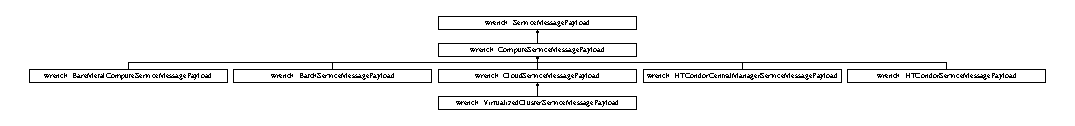
\includegraphics[height=1.247911cm]{classwrench_1_1_compute_service_message_payload}
\end{center}
\end{figure}
\subsection*{Static Public Attributes}
\begin{DoxyCompactItemize}
\item 
\mbox{\Hypertarget{classwrench_1_1_compute_service_message_payload_af1dc4d2c2f784a5b2a29034567254ba7}\label{classwrench_1_1_compute_service_message_payload_af1dc4d2c2f784a5b2a29034567254ba7}} 
static const std\+::string \hyperlink{classwrench_1_1_compute_service_message_payload_af1dc4d2c2f784a5b2a29034567254ba7}{J\+O\+B\+\_\+\+T\+Y\+P\+E\+\_\+\+N\+O\+T\+\_\+\+S\+U\+P\+P\+O\+R\+T\+E\+D\+\_\+\+M\+E\+S\+S\+A\+G\+E\+\_\+\+P\+A\+Y\+L\+O\+AD}
\begin{DoxyCompactList}\small\item\em The number of bytes in the control message sent by the daemon to state that it does not support the type of a submitted job. \end{DoxyCompactList}\item 
\mbox{\Hypertarget{classwrench_1_1_compute_service_message_payload_a1f5b40748d7fe90fb682d735395de3af}\label{classwrench_1_1_compute_service_message_payload_a1f5b40748d7fe90fb682d735395de3af}} 
static const std\+::string \hyperlink{classwrench_1_1_compute_service_message_payload_a1f5b40748d7fe90fb682d735395de3af}{P\+I\+L\+O\+T\+\_\+\+J\+O\+B\+\_\+\+E\+X\+P\+I\+R\+E\+D\+\_\+\+M\+E\+S\+S\+A\+G\+E\+\_\+\+P\+A\+Y\+L\+O\+AD}
\begin{DoxyCompactList}\small\item\em The number of bytes in the control message sent by the daemon to state that a pilot job has expired. \end{DoxyCompactList}\item 
\mbox{\Hypertarget{classwrench_1_1_compute_service_message_payload_a6b614da3139f4735421ed8e918556c0c}\label{classwrench_1_1_compute_service_message_payload_a6b614da3139f4735421ed8e918556c0c}} 
static const std\+::string \hyperlink{classwrench_1_1_compute_service_message_payload_a6b614da3139f4735421ed8e918556c0c}{P\+I\+L\+O\+T\+\_\+\+J\+O\+B\+\_\+\+F\+A\+I\+L\+E\+D\+\_\+\+M\+E\+S\+S\+A\+G\+E\+\_\+\+P\+A\+Y\+L\+O\+AD}
\begin{DoxyCompactList}\small\item\em The number of bytes in the control message sent by the daemon to state that a pilot job has failed. \end{DoxyCompactList}\item 
\mbox{\Hypertarget{classwrench_1_1_compute_service_message_payload_a0a91a957ed0eeba0bb35daea55b25fa5}\label{classwrench_1_1_compute_service_message_payload_a0a91a957ed0eeba0bb35daea55b25fa5}} 
static const std\+::string \hyperlink{classwrench_1_1_compute_service_message_payload_a0a91a957ed0eeba0bb35daea55b25fa5}{P\+I\+L\+O\+T\+\_\+\+J\+O\+B\+\_\+\+S\+T\+A\+R\+T\+E\+D\+\_\+\+M\+E\+S\+S\+A\+G\+E\+\_\+\+P\+A\+Y\+L\+O\+AD}
\begin{DoxyCompactList}\small\item\em The number of bytes in the control message sent by the daemon to state that a pilot job has started. \end{DoxyCompactList}\item 
\mbox{\Hypertarget{classwrench_1_1_compute_service_message_payload_a110f501ef6361a70627833e8ab5ab511}\label{classwrench_1_1_compute_service_message_payload_a110f501ef6361a70627833e8ab5ab511}} 
static const std\+::string \hyperlink{classwrench_1_1_compute_service_message_payload_a110f501ef6361a70627833e8ab5ab511}{R\+E\+S\+O\+U\+R\+C\+E\+\_\+\+D\+E\+S\+C\+R\+I\+P\+T\+I\+O\+N\+\_\+\+A\+N\+S\+W\+E\+R\+\_\+\+M\+E\+S\+S\+A\+G\+E\+\_\+\+P\+A\+Y\+L\+O\+AD}
\begin{DoxyCompactList}\small\item\em The number of bytes in the control message sent by the daemon to state information on its resources. \end{DoxyCompactList}\item 
\mbox{\Hypertarget{classwrench_1_1_compute_service_message_payload_abfd5cdb62efb21fb3ebf7764b9c7ad47}\label{classwrench_1_1_compute_service_message_payload_abfd5cdb62efb21fb3ebf7764b9c7ad47}} 
static const std\+::string \hyperlink{classwrench_1_1_compute_service_message_payload_abfd5cdb62efb21fb3ebf7764b9c7ad47}{R\+E\+S\+O\+U\+R\+C\+E\+\_\+\+D\+E\+S\+C\+R\+I\+P\+T\+I\+O\+N\+\_\+\+R\+E\+Q\+U\+E\+S\+T\+\_\+\+M\+E\+S\+S\+A\+G\+E\+\_\+\+P\+A\+Y\+L\+O\+AD}
\begin{DoxyCompactList}\small\item\em The number of bytes in the control message sent to the daemon to ask it for information on its resources. \end{DoxyCompactList}\item 
\mbox{\Hypertarget{classwrench_1_1_compute_service_message_payload_a3ba0560d8901349f0fbd2ab7e6eb3862}\label{classwrench_1_1_compute_service_message_payload_a3ba0560d8901349f0fbd2ab7e6eb3862}} 
static const std\+::string \hyperlink{classwrench_1_1_compute_service_message_payload_a3ba0560d8901349f0fbd2ab7e6eb3862}{S\+T\+A\+N\+D\+A\+R\+D\+\_\+\+J\+O\+B\+\_\+\+D\+O\+N\+E\+\_\+\+M\+E\+S\+S\+A\+G\+E\+\_\+\+P\+A\+Y\+L\+O\+AD}
\begin{DoxyCompactList}\small\item\em The number of bytes in the control message sent by the daemon to state that it has completed a standard job. \end{DoxyCompactList}\item 
\mbox{\Hypertarget{classwrench_1_1_compute_service_message_payload_aafb88e732f10b7e26bd1fe39356457bf}\label{classwrench_1_1_compute_service_message_payload_aafb88e732f10b7e26bd1fe39356457bf}} 
static const std\+::string \hyperlink{classwrench_1_1_compute_service_message_payload_aafb88e732f10b7e26bd1fe39356457bf}{S\+T\+A\+N\+D\+A\+R\+D\+\_\+\+J\+O\+B\+\_\+\+F\+A\+I\+L\+E\+D\+\_\+\+M\+E\+S\+S\+A\+G\+E\+\_\+\+P\+A\+Y\+L\+O\+AD}
\begin{DoxyCompactList}\small\item\em The number of bytes in the control message sent by the daemon to state that a running standard job has failed. \end{DoxyCompactList}\item 
\mbox{\Hypertarget{classwrench_1_1_compute_service_message_payload_a421715521f0d2837e24e9e150da0de4a}\label{classwrench_1_1_compute_service_message_payload_a421715521f0d2837e24e9e150da0de4a}} 
static const std\+::string \hyperlink{classwrench_1_1_compute_service_message_payload_a421715521f0d2837e24e9e150da0de4a}{S\+U\+B\+M\+I\+T\+\_\+\+P\+I\+L\+O\+T\+\_\+\+J\+O\+B\+\_\+\+A\+N\+S\+W\+E\+R\+\_\+\+M\+E\+S\+S\+A\+G\+E\+\_\+\+P\+A\+Y\+L\+O\+AD}
\begin{DoxyCompactList}\small\item\em The number of bytes in the control message sent from the daemon to acknowledge a pilot job submission. \end{DoxyCompactList}\item 
\mbox{\Hypertarget{classwrench_1_1_compute_service_message_payload_aae15472660475257104b6717902fbffb}\label{classwrench_1_1_compute_service_message_payload_aae15472660475257104b6717902fbffb}} 
static const std\+::string \hyperlink{classwrench_1_1_compute_service_message_payload_aae15472660475257104b6717902fbffb}{S\+U\+B\+M\+I\+T\+\_\+\+P\+I\+L\+O\+T\+\_\+\+J\+O\+B\+\_\+\+R\+E\+Q\+U\+E\+S\+T\+\_\+\+M\+E\+S\+S\+A\+G\+E\+\_\+\+P\+A\+Y\+L\+O\+AD}
\begin{DoxyCompactList}\small\item\em The number of bytes in the control message sent to the daemon to submit a pilot job. \end{DoxyCompactList}\item 
\mbox{\Hypertarget{classwrench_1_1_compute_service_message_payload_a1c23509b24aee6ea4e71b28497d659ba}\label{classwrench_1_1_compute_service_message_payload_a1c23509b24aee6ea4e71b28497d659ba}} 
static const std\+::string \hyperlink{classwrench_1_1_compute_service_message_payload_a1c23509b24aee6ea4e71b28497d659ba}{S\+U\+B\+M\+I\+T\+\_\+\+S\+T\+A\+N\+D\+A\+R\+D\+\_\+\+J\+O\+B\+\_\+\+A\+N\+S\+W\+E\+R\+\_\+\+M\+E\+S\+S\+A\+G\+E\+\_\+\+P\+A\+Y\+L\+O\+AD}
\begin{DoxyCompactList}\small\item\em The number of bytes in the control message sent by the daemon to acknowledge a standard job submission. \end{DoxyCompactList}\item 
\mbox{\Hypertarget{classwrench_1_1_compute_service_message_payload_a86cb39a4741f03121d6c8254d8cbaf1c}\label{classwrench_1_1_compute_service_message_payload_a86cb39a4741f03121d6c8254d8cbaf1c}} 
static const std\+::string \hyperlink{classwrench_1_1_compute_service_message_payload_a86cb39a4741f03121d6c8254d8cbaf1c}{S\+U\+B\+M\+I\+T\+\_\+\+S\+T\+A\+N\+D\+A\+R\+D\+\_\+\+J\+O\+B\+\_\+\+R\+E\+Q\+U\+E\+S\+T\+\_\+\+M\+E\+S\+S\+A\+G\+E\+\_\+\+P\+A\+Y\+L\+O\+AD}
\begin{DoxyCompactList}\small\item\em The number of bytes in the control message sent to the daemon to submit a standard job. \end{DoxyCompactList}\item 
\mbox{\Hypertarget{classwrench_1_1_compute_service_message_payload_ad0bf94135d0c642785f4ce490a0dde0b}\label{classwrench_1_1_compute_service_message_payload_ad0bf94135d0c642785f4ce490a0dde0b}} 
static const std\+::string \hyperlink{classwrench_1_1_compute_service_message_payload_ad0bf94135d0c642785f4ce490a0dde0b}{T\+E\+R\+M\+I\+N\+A\+T\+E\+\_\+\+P\+I\+L\+O\+T\+\_\+\+J\+O\+B\+\_\+\+A\+N\+S\+W\+E\+R\+\_\+\+M\+E\+S\+S\+A\+G\+E\+\_\+\+P\+A\+Y\+L\+O\+AD}
\begin{DoxyCompactList}\small\item\em The number of bytes in the control message sent by the daemon to acknowledge a pilot job termination. \end{DoxyCompactList}\item 
\mbox{\Hypertarget{classwrench_1_1_compute_service_message_payload_a6d80bf772eba3b8eb7224dc73e370cd0}\label{classwrench_1_1_compute_service_message_payload_a6d80bf772eba3b8eb7224dc73e370cd0}} 
static const std\+::string \hyperlink{classwrench_1_1_compute_service_message_payload_a6d80bf772eba3b8eb7224dc73e370cd0}{T\+E\+R\+M\+I\+N\+A\+T\+E\+\_\+\+P\+I\+L\+O\+T\+\_\+\+J\+O\+B\+\_\+\+R\+E\+Q\+U\+E\+S\+T\+\_\+\+M\+E\+S\+S\+A\+G\+E\+\_\+\+P\+A\+Y\+L\+O\+AD}
\begin{DoxyCompactList}\small\item\em The number of bytes in the control message sent to the daemon to terminate a pilot job. \end{DoxyCompactList}\item 
\mbox{\Hypertarget{classwrench_1_1_compute_service_message_payload_a734ce7db76ab5ec58a6c692ce4b8e18f}\label{classwrench_1_1_compute_service_message_payload_a734ce7db76ab5ec58a6c692ce4b8e18f}} 
static const std\+::string \hyperlink{classwrench_1_1_compute_service_message_payload_a734ce7db76ab5ec58a6c692ce4b8e18f}{T\+E\+R\+M\+I\+N\+A\+T\+E\+\_\+\+S\+T\+A\+N\+D\+A\+R\+D\+\_\+\+J\+O\+B\+\_\+\+A\+N\+S\+W\+E\+R\+\_\+\+M\+E\+S\+S\+A\+G\+E\+\_\+\+P\+A\+Y\+L\+O\+AD}
\begin{DoxyCompactList}\small\item\em The number of bytes in the control message sent by the daemon to acknowledge a standard job termination. \end{DoxyCompactList}\item 
\mbox{\Hypertarget{classwrench_1_1_compute_service_message_payload_a24f99e315abb2e89e666e719af98d4dc}\label{classwrench_1_1_compute_service_message_payload_a24f99e315abb2e89e666e719af98d4dc}} 
static const std\+::string \hyperlink{classwrench_1_1_compute_service_message_payload_a24f99e315abb2e89e666e719af98d4dc}{T\+E\+R\+M\+I\+N\+A\+T\+E\+\_\+\+S\+T\+A\+N\+D\+A\+R\+D\+\_\+\+J\+O\+B\+\_\+\+R\+E\+Q\+U\+E\+S\+T\+\_\+\+M\+E\+S\+S\+A\+G\+E\+\_\+\+P\+A\+Y\+L\+O\+AD}
\begin{DoxyCompactList}\small\item\em The number of bytes in the control message sent to the daemon to terminate a standard job. \end{DoxyCompactList}\item 
\mbox{\Hypertarget{classwrench_1_1_compute_service_message_payload_a79d0d40e02d24145252b7afb2c526cc5}\label{classwrench_1_1_compute_service_message_payload_a79d0d40e02d24145252b7afb2c526cc5}} 
static const std\+::string \hyperlink{classwrench_1_1_compute_service_message_payload_a79d0d40e02d24145252b7afb2c526cc5}{T\+T\+L\+\_\+\+A\+N\+S\+W\+E\+R\+\_\+\+M\+E\+S\+S\+A\+G\+E\+\_\+\+P\+A\+Y\+L\+O\+AD}
\begin{DoxyCompactList}\small\item\em The number of bytes in the control message sent by the daemon to state its time-\/to-\/live. \end{DoxyCompactList}\item 
\mbox{\Hypertarget{classwrench_1_1_compute_service_message_payload_a951187b1bb9fb20d7944e5577b94ae47}\label{classwrench_1_1_compute_service_message_payload_a951187b1bb9fb20d7944e5577b94ae47}} 
static const std\+::string \hyperlink{classwrench_1_1_compute_service_message_payload_a951187b1bb9fb20d7944e5577b94ae47}{T\+T\+L\+\_\+\+R\+E\+Q\+U\+E\+S\+T\+\_\+\+M\+E\+S\+S\+A\+G\+E\+\_\+\+P\+A\+Y\+L\+O\+AD}
\begin{DoxyCompactList}\small\item\em The number of bytes in the control message sent to the daemon to ask it for its time-\/to-\/live. \end{DoxyCompactList}\end{DoxyCompactItemize}


\subsection{Detailed Description}
Configurable message payloads for a \hyperlink{classwrench_1_1_compute_service}{Compute\+Service}. 

The documentation for this class was generated from the following file\+:\begin{DoxyCompactItemize}
\item 
/\+Users/rafsilva/\+Documents/isi/workspace/wrench/wrench/include/wrench/services/compute/Compute\+Service\+Message\+Payload.\+h\end{DoxyCompactItemize}

\hypertarget{classwrench_1_1_compute_service_property}{}\section{wrench\+:\+:Compute\+Service\+Property Class Reference}
\label{classwrench_1_1_compute_service_property}\index{wrench\+::\+Compute\+Service\+Property@{wrench\+::\+Compute\+Service\+Property}}


Configurable properties for a \hyperlink{classwrench_1_1_compute_service}{Compute\+Service}.  




{\ttfamily \#include $<$Compute\+Service\+Property.\+h$>$}

Inheritance diagram for wrench\+:\+:Compute\+Service\+Property\+:\begin{figure}[H]
\begin{center}
\leavevmode
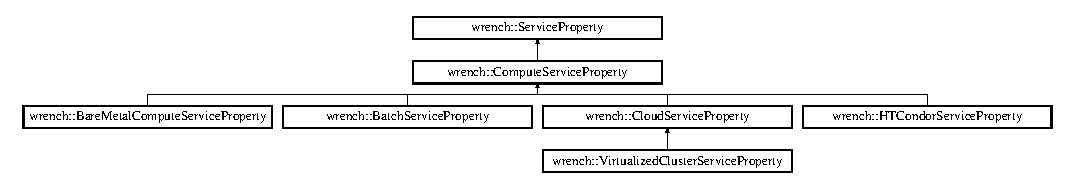
\includegraphics[height=2.089552cm]{classwrench_1_1_compute_service_property}
\end{center}
\end{figure}
\subsection*{Static Public Attributes}
\begin{DoxyCompactItemize}
\item 
\mbox{\Hypertarget{classwrench_1_1_compute_service_property_af0abab1e3bce4932c4482031f0c31ce8}\label{classwrench_1_1_compute_service_property_af0abab1e3bce4932c4482031f0c31ce8}} 
static const std\+::string \hyperlink{classwrench_1_1_compute_service_property_af0abab1e3bce4932c4482031f0c31ce8}{S\+U\+P\+P\+O\+R\+T\+S\+\_\+\+P\+I\+L\+O\+T\+\_\+\+J\+O\+BS}
\begin{DoxyCompactList}\small\item\em Whether the compute service supports pilot jobs (true or false) \end{DoxyCompactList}\item 
\mbox{\Hypertarget{classwrench_1_1_compute_service_property_a4e1b5e2e1effa86cfac0da608f112c14}\label{classwrench_1_1_compute_service_property_a4e1b5e2e1effa86cfac0da608f112c14}} 
static const std\+::string \hyperlink{classwrench_1_1_compute_service_property_a4e1b5e2e1effa86cfac0da608f112c14}{S\+U\+P\+P\+O\+R\+T\+S\+\_\+\+S\+T\+A\+N\+D\+A\+R\+D\+\_\+\+J\+O\+BS}
\begin{DoxyCompactList}\small\item\em Whether the compute service supports standard jobs (true or false) \end{DoxyCompactList}\end{DoxyCompactItemize}


\subsection{Detailed Description}
Configurable properties for a \hyperlink{classwrench_1_1_compute_service}{Compute\+Service}. 

The documentation for this class was generated from the following file\+:\begin{DoxyCompactItemize}
\item 
/\+Users/rafsilva/\+Documents/isi/workspace/wrench/wrench/include/wrench/services/compute/Compute\+Service\+Property.\+h\end{DoxyCompactItemize}

\hypertarget{classwrench_1_1_compute_thread_has_died}{}\section{wrench\+:\+:Compute\+Thread\+Has\+Died Class Reference}
\label{classwrench_1_1_compute_thread_has_died}\index{wrench\+::\+Compute\+Thread\+Has\+Died@{wrench\+::\+Compute\+Thread\+Has\+Died}}


A \char`\"{}compute thread has died\char`\"{} failure cause.  




{\ttfamily \#include $<$Failure\+Cause.\+h$>$}

Inheritance diagram for wrench\+:\+:Compute\+Thread\+Has\+Died\+:\begin{figure}[H]
\begin{center}
\leavevmode
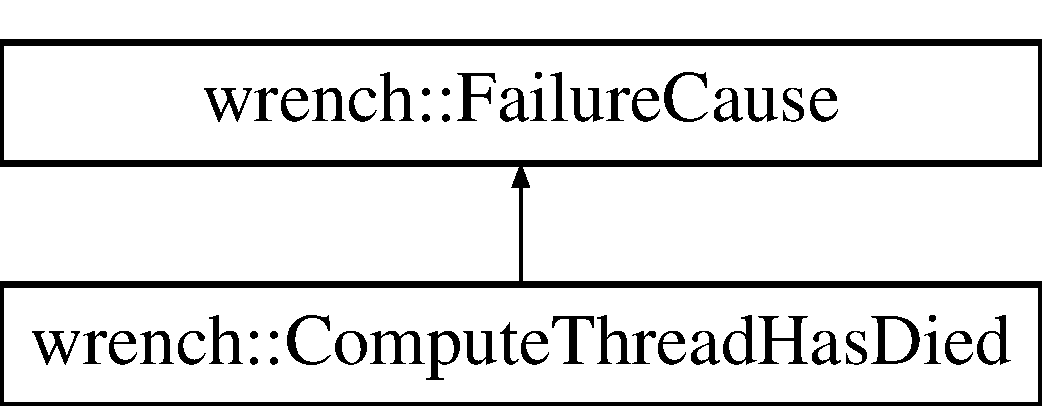
\includegraphics[height=2.000000cm]{classwrench_1_1_compute_thread_has_died}
\end{center}
\end{figure}
\subsection*{Public Member Functions}
\begin{DoxyCompactItemize}
\item 
std\+::string \hyperlink{classwrench_1_1_compute_thread_has_died_a4725416d9ff31b39ec9d48d23d1c1c0b}{to\+String} ()
\begin{DoxyCompactList}\small\item\em Get the human-\/readable failure message. \end{DoxyCompactList}\end{DoxyCompactItemize}
\subsection*{Additional Inherited Members}


\subsection{Detailed Description}
A \char`\"{}compute thread has died\char`\"{} failure cause. 

\subsection{Member Function Documentation}
\mbox{\Hypertarget{classwrench_1_1_compute_thread_has_died_a4725416d9ff31b39ec9d48d23d1c1c0b}\label{classwrench_1_1_compute_thread_has_died_a4725416d9ff31b39ec9d48d23d1c1c0b}} 
\index{wrench\+::\+Compute\+Thread\+Has\+Died@{wrench\+::\+Compute\+Thread\+Has\+Died}!to\+String@{to\+String}}
\index{to\+String@{to\+String}!wrench\+::\+Compute\+Thread\+Has\+Died@{wrench\+::\+Compute\+Thread\+Has\+Died}}
\subsubsection{\texorpdfstring{to\+String()}{toString()}}
{\footnotesize\ttfamily std\+::string wrench\+::\+Compute\+Thread\+Has\+Died\+::to\+String (\begin{DoxyParamCaption}{ }\end{DoxyParamCaption})\hspace{0.3cm}{\ttfamily [virtual]}}



Get the human-\/readable failure message. 

\begin{DoxyReturn}{Returns}
the message 
\end{DoxyReturn}


Implements \hyperlink{classwrench_1_1_failure_cause_afbad248ebe902409f2cd4f1d6f2b867d}{wrench\+::\+Failure\+Cause}.



The documentation for this class was generated from the following files\+:\begin{DoxyCompactItemize}
\item 
/\+Users/rafsilva/\+Documents/isi/workspace/wrench/wrench/include/wrench/workflow/execution\+\_\+events/Failure\+Cause.\+h\item 
/\+Users/rafsilva/\+Documents/isi/workspace/wrench/wrench/src/wrench/workflow/execution\+\_\+events/Failure\+Cause.\+cpp\end{DoxyCompactItemize}

\hypertarget{classwrench_1_1_data_movement_manager}{}\section{wrench\+:\+:Data\+Movement\+Manager Class Reference}
\label{classwrench_1_1_data_movement_manager}\index{wrench\+::\+Data\+Movement\+Manager@{wrench\+::\+Data\+Movement\+Manager}}


A helper daemon (co-\/located with a \hyperlink{classwrench_1_1_w_m_s}{W\+MS}) that handles data movement operations.  




{\ttfamily \#include $<$Data\+Movement\+Manager.\+h$>$}

Inheritance diagram for wrench\+:\+:Data\+Movement\+Manager\+:\begin{figure}[H]
\begin{center}
\leavevmode
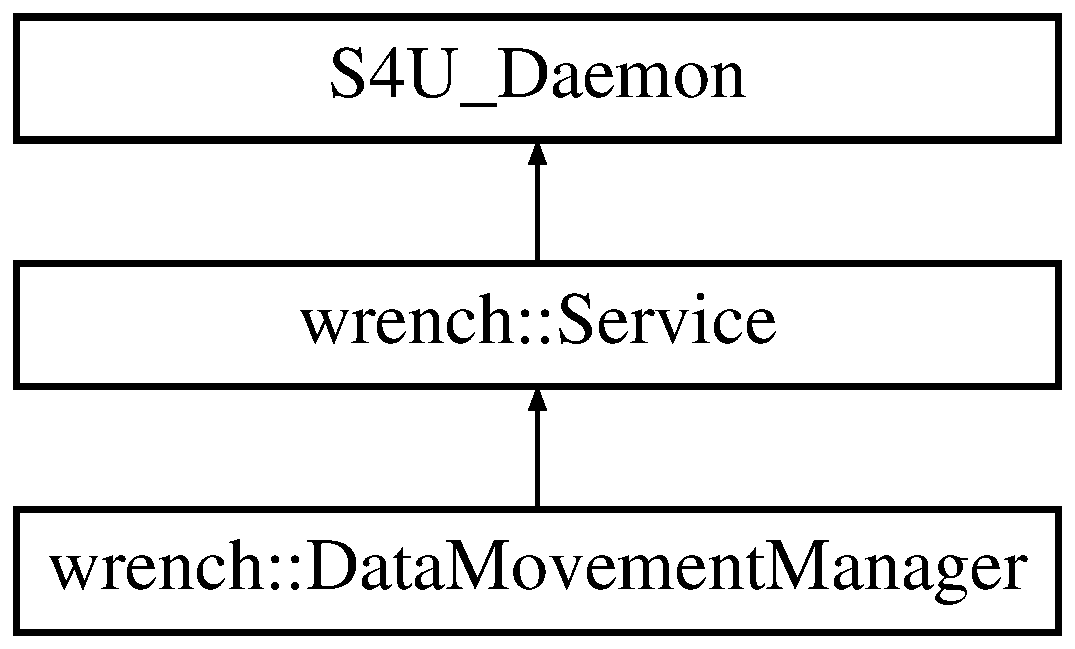
\includegraphics[height=3.000000cm]{classwrench_1_1_data_movement_manager}
\end{center}
\end{figure}
\subsection*{Public Member Functions}
\begin{DoxyCompactItemize}
\item 
void \hyperlink{classwrench_1_1_data_movement_manager_a815bf4ed2a32b39c0e46a6f5a3c10e51}{do\+Synchronous\+File\+Copy} (\hyperlink{classwrench_1_1_workflow_file}{Workflow\+File} $\ast$file, \hyperlink{classwrench_1_1_storage_service}{Storage\+Service} $\ast$src, \hyperlink{classwrench_1_1_storage_service}{Storage\+Service} $\ast$dst, \hyperlink{classwrench_1_1_file_registry_service}{File\+Registry\+Service} $\ast$file\+\_\+registry\+\_\+service=nullptr)
\begin{DoxyCompactList}\small\item\em Ask the data manager to perform a synchronous file copy. \end{DoxyCompactList}\item 
void \hyperlink{classwrench_1_1_data_movement_manager_ad9c2dd49c769884e01932df7ac90bb0e}{do\+Synchronous\+File\+Copy} (\hyperlink{classwrench_1_1_workflow_file}{Workflow\+File} $\ast$file, \hyperlink{classwrench_1_1_storage_service}{Storage\+Service} $\ast$src, std\+::string src\+\_\+partition, \hyperlink{classwrench_1_1_storage_service}{Storage\+Service} $\ast$dst, std\+::string dst\+\_\+partition, \hyperlink{classwrench_1_1_file_registry_service}{File\+Registry\+Service} $\ast$file\+\_\+registry\+\_\+service=nullptr)
\begin{DoxyCompactList}\small\item\em Ask the data manager to perform a synchronous file copy. \end{DoxyCompactList}\item 
void \hyperlink{classwrench_1_1_data_movement_manager_a3ddeb9700a10b5f249b91786e6dddcb0}{initiate\+Asynchronous\+File\+Copy} (\hyperlink{classwrench_1_1_workflow_file}{Workflow\+File} $\ast$file, \hyperlink{classwrench_1_1_storage_service}{Storage\+Service} $\ast$src, \hyperlink{classwrench_1_1_storage_service}{Storage\+Service} $\ast$dst, \hyperlink{classwrench_1_1_file_registry_service}{File\+Registry\+Service} $\ast$file\+\_\+registry\+\_\+service=nullptr)
\begin{DoxyCompactList}\small\item\em Ask the data manager to initiate an asynchronous file copy. \end{DoxyCompactList}\item 
void \hyperlink{classwrench_1_1_data_movement_manager_a87d7d38e2d45b6024789feac0213d0b2}{initiate\+Asynchronous\+File\+Copy} (\hyperlink{classwrench_1_1_workflow_file}{Workflow\+File} $\ast$file, \hyperlink{classwrench_1_1_storage_service}{Storage\+Service} $\ast$src, std\+::string src\+\_\+partition, \hyperlink{classwrench_1_1_storage_service}{Storage\+Service} $\ast$dst, std\+::string dst\+\_\+partition, \hyperlink{classwrench_1_1_file_registry_service}{File\+Registry\+Service} $\ast$file\+\_\+registry\+\_\+service=nullptr)
\begin{DoxyCompactList}\small\item\em Ask the data manager to initiate an asynchronous file copy. \end{DoxyCompactList}\item 
\mbox{\Hypertarget{classwrench_1_1_data_movement_manager_a231a54a5b09f83f8e6e9681cc3134864}\label{classwrench_1_1_data_movement_manager_a231a54a5b09f83f8e6e9681cc3134864}} 
void \hyperlink{classwrench_1_1_data_movement_manager_a231a54a5b09f83f8e6e9681cc3134864}{kill} ()
\begin{DoxyCompactList}\small\item\em Kill the manager (brutally terminate the daemon) \end{DoxyCompactList}\item 
void \hyperlink{classwrench_1_1_data_movement_manager_a72fc97280a6f1f475e168c1f71ec5f70}{stop} ()
\begin{DoxyCompactList}\small\item\em Stop the manager. \end{DoxyCompactList}\end{DoxyCompactItemize}
\subsection*{Protected Member Functions}
\begin{DoxyCompactItemize}
\item 
\hyperlink{classwrench_1_1_data_movement_manager_aef4b101f450be0869b60dc5d656dcf1e}{Data\+Movement\+Manager} (\hyperlink{classwrench_1_1_w_m_s}{W\+MS} $\ast$wms)
\begin{DoxyCompactList}\small\item\em Constructor. \end{DoxyCompactList}\end{DoxyCompactItemize}
\subsection*{Additional Inherited Members}


\subsection{Detailed Description}
A helper daemon (co-\/located with a \hyperlink{classwrench_1_1_w_m_s}{W\+MS}) that handles data movement operations. 

\subsection{Constructor \& Destructor Documentation}
\mbox{\Hypertarget{classwrench_1_1_data_movement_manager_aef4b101f450be0869b60dc5d656dcf1e}\label{classwrench_1_1_data_movement_manager_aef4b101f450be0869b60dc5d656dcf1e}} 
\index{wrench\+::\+Data\+Movement\+Manager@{wrench\+::\+Data\+Movement\+Manager}!Data\+Movement\+Manager@{Data\+Movement\+Manager}}
\index{Data\+Movement\+Manager@{Data\+Movement\+Manager}!wrench\+::\+Data\+Movement\+Manager@{wrench\+::\+Data\+Movement\+Manager}}
\subsubsection{\texorpdfstring{Data\+Movement\+Manager()}{DataMovementManager()}}
{\footnotesize\ttfamily wrench\+::\+Data\+Movement\+Manager\+::\+Data\+Movement\+Manager (\begin{DoxyParamCaption}\item[{\hyperlink{classwrench_1_1_w_m_s}{W\+MS} $\ast$}]{wms }\end{DoxyParamCaption})\hspace{0.3cm}{\ttfamily [explicit]}, {\ttfamily [protected]}}



Constructor. 


\begin{DoxyParams}{Parameters}
{\em wms} & the \hyperlink{classwrench_1_1_w_m_s}{W\+MS} that uses this data movement manager \\
\hline
\end{DoxyParams}


\subsection{Member Function Documentation}
\mbox{\Hypertarget{classwrench_1_1_data_movement_manager_a815bf4ed2a32b39c0e46a6f5a3c10e51}\label{classwrench_1_1_data_movement_manager_a815bf4ed2a32b39c0e46a6f5a3c10e51}} 
\index{wrench\+::\+Data\+Movement\+Manager@{wrench\+::\+Data\+Movement\+Manager}!do\+Synchronous\+File\+Copy@{do\+Synchronous\+File\+Copy}}
\index{do\+Synchronous\+File\+Copy@{do\+Synchronous\+File\+Copy}!wrench\+::\+Data\+Movement\+Manager@{wrench\+::\+Data\+Movement\+Manager}}
\subsubsection{\texorpdfstring{do\+Synchronous\+File\+Copy()}{doSynchronousFileCopy()}\hspace{0.1cm}{\footnotesize\ttfamily [1/2]}}
{\footnotesize\ttfamily void wrench\+::\+Data\+Movement\+Manager\+::do\+Synchronous\+File\+Copy (\begin{DoxyParamCaption}\item[{\hyperlink{classwrench_1_1_workflow_file}{Workflow\+File} $\ast$}]{file,  }\item[{\hyperlink{classwrench_1_1_storage_service}{Storage\+Service} $\ast$}]{src,  }\item[{\hyperlink{classwrench_1_1_storage_service}{Storage\+Service} $\ast$}]{dst,  }\item[{\hyperlink{classwrench_1_1_file_registry_service}{File\+Registry\+Service} $\ast$}]{file\+\_\+registry\+\_\+service = {\ttfamily nullptr} }\end{DoxyParamCaption})}



Ask the data manager to perform a synchronous file copy. 


\begin{DoxyParams}{Parameters}
{\em file} & the file to copy \\
\hline
{\em src} & the source storage service (using the \char`\"{}/\char`\"{} partition) \\
\hline
{\em dst} & the destination storage service (using the \char`\"{}/\char`\"{} partition) \\
\hline
{\em file\+\_\+registry\+\_\+service} & a file registry service to update once the file copy has (successfully) completed (none if nullptr)\\
\hline
\end{DoxyParams}

\begin{DoxyExceptions}{Exceptions}
{\em std\+::invalid\+\_\+argument} & \\
\hline
{\em \hyperlink{classwrench_1_1_workflow_execution_exception}{Workflow\+Execution\+Exception}} & \\
\hline
\end{DoxyExceptions}
\mbox{\Hypertarget{classwrench_1_1_data_movement_manager_ad9c2dd49c769884e01932df7ac90bb0e}\label{classwrench_1_1_data_movement_manager_ad9c2dd49c769884e01932df7ac90bb0e}} 
\index{wrench\+::\+Data\+Movement\+Manager@{wrench\+::\+Data\+Movement\+Manager}!do\+Synchronous\+File\+Copy@{do\+Synchronous\+File\+Copy}}
\index{do\+Synchronous\+File\+Copy@{do\+Synchronous\+File\+Copy}!wrench\+::\+Data\+Movement\+Manager@{wrench\+::\+Data\+Movement\+Manager}}
\subsubsection{\texorpdfstring{do\+Synchronous\+File\+Copy()}{doSynchronousFileCopy()}\hspace{0.1cm}{\footnotesize\ttfamily [2/2]}}
{\footnotesize\ttfamily void wrench\+::\+Data\+Movement\+Manager\+::do\+Synchronous\+File\+Copy (\begin{DoxyParamCaption}\item[{\hyperlink{classwrench_1_1_workflow_file}{Workflow\+File} $\ast$}]{file,  }\item[{\hyperlink{classwrench_1_1_storage_service}{Storage\+Service} $\ast$}]{src,  }\item[{std\+::string}]{src\+\_\+partition,  }\item[{\hyperlink{classwrench_1_1_storage_service}{Storage\+Service} $\ast$}]{dst,  }\item[{std\+::string}]{dst\+\_\+partition,  }\item[{\hyperlink{classwrench_1_1_file_registry_service}{File\+Registry\+Service} $\ast$}]{file\+\_\+registry\+\_\+service = {\ttfamily nullptr} }\end{DoxyParamCaption})}



Ask the data manager to perform a synchronous file copy. 


\begin{DoxyParams}{Parameters}
{\em file} & the file to copy \\
\hline
{\em src} & the source storage service \\
\hline
{\em dst} & the destination storage service \\
\hline
{\em file\+\_\+registry\+\_\+service} & a file registry service to update once the file copy has (successfully) completed (none if nullptr)\\
\hline
\end{DoxyParams}

\begin{DoxyExceptions}{Exceptions}
{\em std\+::invalid\+\_\+argument} & \\
\hline
{\em \hyperlink{classwrench_1_1_workflow_execution_exception}{Workflow\+Execution\+Exception}} & \\
\hline
\end{DoxyExceptions}
\mbox{\Hypertarget{classwrench_1_1_data_movement_manager_a3ddeb9700a10b5f249b91786e6dddcb0}\label{classwrench_1_1_data_movement_manager_a3ddeb9700a10b5f249b91786e6dddcb0}} 
\index{wrench\+::\+Data\+Movement\+Manager@{wrench\+::\+Data\+Movement\+Manager}!initiate\+Asynchronous\+File\+Copy@{initiate\+Asynchronous\+File\+Copy}}
\index{initiate\+Asynchronous\+File\+Copy@{initiate\+Asynchronous\+File\+Copy}!wrench\+::\+Data\+Movement\+Manager@{wrench\+::\+Data\+Movement\+Manager}}
\subsubsection{\texorpdfstring{initiate\+Asynchronous\+File\+Copy()}{initiateAsynchronousFileCopy()}\hspace{0.1cm}{\footnotesize\ttfamily [1/2]}}
{\footnotesize\ttfamily void wrench\+::\+Data\+Movement\+Manager\+::initiate\+Asynchronous\+File\+Copy (\begin{DoxyParamCaption}\item[{\hyperlink{classwrench_1_1_workflow_file}{Workflow\+File} $\ast$}]{file,  }\item[{\hyperlink{classwrench_1_1_storage_service}{Storage\+Service} $\ast$}]{src,  }\item[{\hyperlink{classwrench_1_1_storage_service}{Storage\+Service} $\ast$}]{dst,  }\item[{\hyperlink{classwrench_1_1_file_registry_service}{File\+Registry\+Service} $\ast$}]{file\+\_\+registry\+\_\+service = {\ttfamily nullptr} }\end{DoxyParamCaption})}



Ask the data manager to initiate an asynchronous file copy. 


\begin{DoxyParams}{Parameters}
{\em file} & the file to copy \\
\hline
{\em src} & the source storage service (using the \char`\"{}/\char`\"{} partition) \\
\hline
{\em dst} & the destination storage service (using the \char`\"{}/\char`\"{} partition) \\
\hline
{\em file\+\_\+registry\+\_\+service} & a file registry service to update once the file copy has (successfully) completed (none if nullptr)\\
\hline
\end{DoxyParams}

\begin{DoxyExceptions}{Exceptions}
{\em std\+::invalid\+\_\+argument} & \\
\hline
{\em \hyperlink{classwrench_1_1_workflow_execution_exception}{Workflow\+Execution\+Exception}} & \\
\hline
\end{DoxyExceptions}
\mbox{\Hypertarget{classwrench_1_1_data_movement_manager_a87d7d38e2d45b6024789feac0213d0b2}\label{classwrench_1_1_data_movement_manager_a87d7d38e2d45b6024789feac0213d0b2}} 
\index{wrench\+::\+Data\+Movement\+Manager@{wrench\+::\+Data\+Movement\+Manager}!initiate\+Asynchronous\+File\+Copy@{initiate\+Asynchronous\+File\+Copy}}
\index{initiate\+Asynchronous\+File\+Copy@{initiate\+Asynchronous\+File\+Copy}!wrench\+::\+Data\+Movement\+Manager@{wrench\+::\+Data\+Movement\+Manager}}
\subsubsection{\texorpdfstring{initiate\+Asynchronous\+File\+Copy()}{initiateAsynchronousFileCopy()}\hspace{0.1cm}{\footnotesize\ttfamily [2/2]}}
{\footnotesize\ttfamily void wrench\+::\+Data\+Movement\+Manager\+::initiate\+Asynchronous\+File\+Copy (\begin{DoxyParamCaption}\item[{\hyperlink{classwrench_1_1_workflow_file}{Workflow\+File} $\ast$}]{file,  }\item[{\hyperlink{classwrench_1_1_storage_service}{Storage\+Service} $\ast$}]{src,  }\item[{std\+::string}]{src\+\_\+partition,  }\item[{\hyperlink{classwrench_1_1_storage_service}{Storage\+Service} $\ast$}]{dst,  }\item[{std\+::string}]{dst\+\_\+partition,  }\item[{\hyperlink{classwrench_1_1_file_registry_service}{File\+Registry\+Service} $\ast$}]{file\+\_\+registry\+\_\+service = {\ttfamily nullptr} }\end{DoxyParamCaption})}



Ask the data manager to initiate an asynchronous file copy. 


\begin{DoxyParams}{Parameters}
{\em file} & the file to copy \\
\hline
{\em src} & the source storage service \\
\hline
{\em src\+\_\+partition} & the source partition \\
\hline
{\em dst} & the destination storage service \\
\hline
{\em dst\+\_\+partition} & the destination partition \\
\hline
{\em file\+\_\+registry\+\_\+service} & a file registry service to update once the file copy has (successfully) completed (none if nullptr)\\
\hline
\end{DoxyParams}

\begin{DoxyExceptions}{Exceptions}
{\em std\+::invalid\+\_\+argument} & \\
\hline
{\em \hyperlink{classwrench_1_1_workflow_execution_exception}{Workflow\+Execution\+Exception}} & \\
\hline
\end{DoxyExceptions}
\mbox{\Hypertarget{classwrench_1_1_data_movement_manager_a72fc97280a6f1f475e168c1f71ec5f70}\label{classwrench_1_1_data_movement_manager_a72fc97280a6f1f475e168c1f71ec5f70}} 
\index{wrench\+::\+Data\+Movement\+Manager@{wrench\+::\+Data\+Movement\+Manager}!stop@{stop}}
\index{stop@{stop}!wrench\+::\+Data\+Movement\+Manager@{wrench\+::\+Data\+Movement\+Manager}}
\subsubsection{\texorpdfstring{stop()}{stop()}}
{\footnotesize\ttfamily void wrench\+::\+Data\+Movement\+Manager\+::stop (\begin{DoxyParamCaption}{ }\end{DoxyParamCaption})\hspace{0.3cm}{\ttfamily [virtual]}}



Stop the manager. 


\begin{DoxyExceptions}{Exceptions}
{\em \hyperlink{classwrench_1_1_workflow_execution_exception}{Workflow\+Execution\+Exception}} & \\
\hline
{\em std\+::runtime\+\_\+error} & \\
\hline
\end{DoxyExceptions}


Reimplemented from \hyperlink{classwrench_1_1_service_ac33a32f4758c6f51b27d2cfb9b46efda}{wrench\+::\+Service}.



The documentation for this class was generated from the following files\+:\begin{DoxyCompactItemize}
\item 
/\+Users/rafsilva/\+Documents/isi/workspace/wrench/wrench/include/wrench/managers/Data\+Movement\+Manager.\+h\item 
/\+Users/rafsilva/\+Documents/isi/workspace/wrench/wrench/src/wrench/managers/Data\+Movement\+Manager.\+cpp\end{DoxyCompactItemize}

\hypertarget{classwrench_1_1_dynamic_optimization}{}\section{wrench\+:\+:Dynamic\+Optimization Class Reference}
\label{classwrench_1_1_dynamic_optimization}\index{wrench\+::\+Dynamic\+Optimization@{wrench\+::\+Dynamic\+Optimization}}


An abstract class that serves as a base class for implementing dynamic (i.\+e., at runtime) optimizations to be used by a \hyperlink{classwrench_1_1_w_m_s}{W\+MS} while executing a \hyperlink{classwrench_1_1_workflow}{Workflow}.  




{\ttfamily \#include $<$Dynamic\+Optimization.\+h$>$}

\subsection*{Public Member Functions}
\begin{DoxyCompactItemize}
\item 
virtual void \hyperlink{classwrench_1_1_dynamic_optimization_a996a15c4c05df94fdf01303bea4bb6aa}{process} (\hyperlink{classwrench_1_1_workflow}{Workflow} $\ast$workflow)=0
\begin{DoxyCompactList}\small\item\em Method to process (i.\+e., modify the structure of) a workflow at runtime so as to optimize its execution (to be overridden) \end{DoxyCompactList}\end{DoxyCompactItemize}


\subsection{Detailed Description}
An abstract class that serves as a base class for implementing dynamic (i.\+e., at runtime) optimizations to be used by a \hyperlink{classwrench_1_1_w_m_s}{W\+MS} while executing a \hyperlink{classwrench_1_1_workflow}{Workflow}. 

\subsection{Member Function Documentation}
\mbox{\Hypertarget{classwrench_1_1_dynamic_optimization_a996a15c4c05df94fdf01303bea4bb6aa}\label{classwrench_1_1_dynamic_optimization_a996a15c4c05df94fdf01303bea4bb6aa}} 
\index{wrench\+::\+Dynamic\+Optimization@{wrench\+::\+Dynamic\+Optimization}!process@{process}}
\index{process@{process}!wrench\+::\+Dynamic\+Optimization@{wrench\+::\+Dynamic\+Optimization}}
\subsubsection{\texorpdfstring{process()}{process()}}
{\footnotesize\ttfamily virtual void wrench\+::\+Dynamic\+Optimization\+::process (\begin{DoxyParamCaption}\item[{\hyperlink{classwrench_1_1_workflow}{Workflow} $\ast$}]{workflow }\end{DoxyParamCaption})\hspace{0.3cm}{\ttfamily [pure virtual]}}



Method to process (i.\+e., modify the structure of) a workflow at runtime so as to optimize its execution (to be overridden) 


\begin{DoxyParams}{Parameters}
{\em workflow} & the workflow \\
\hline
\end{DoxyParams}


The documentation for this class was generated from the following file\+:\begin{DoxyCompactItemize}
\item 
/\+Users/rafsilva/\+Documents/isi/workspace/wrench/wrench/include/wrench/wms/Dynamic\+Optimization.\+h\end{DoxyCompactItemize}

\hypertarget{classwrench_1_1_energy_meter}{}\section{wrench\+:\+:Energy\+Meter Class Reference}
\label{classwrench_1_1_energy_meter}\index{wrench\+::\+Energy\+Meter@{wrench\+::\+Energy\+Meter}}
Inheritance diagram for wrench\+:\+:Energy\+Meter\+:\begin{figure}[H]
\begin{center}
\leavevmode
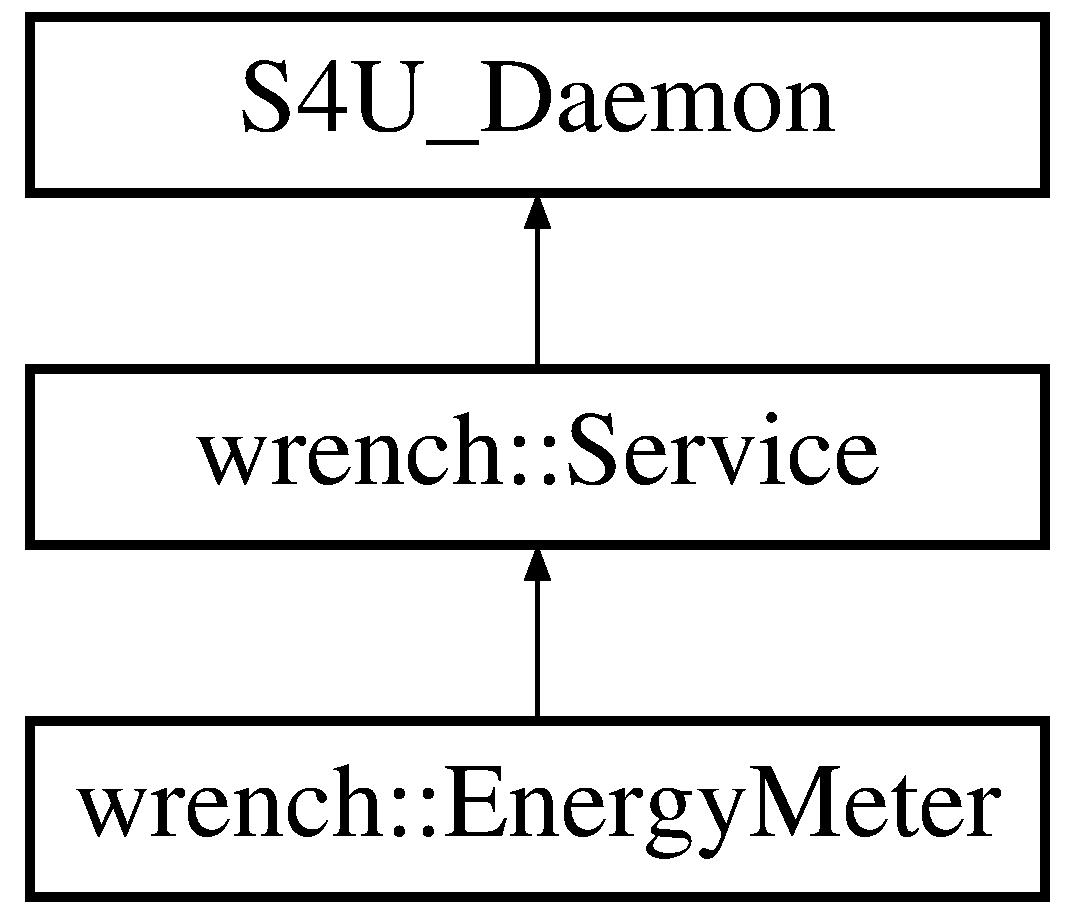
\includegraphics[height=3.000000cm]{classwrench_1_1_energy_meter}
\end{center}
\end{figure}
\subsection*{Public Member Functions}
\begin{DoxyCompactItemize}
\item 
\mbox{\Hypertarget{classwrench_1_1_energy_meter_a2f39104adc8875ae269dea7c58b5aa06}\label{classwrench_1_1_energy_meter_a2f39104adc8875ae269dea7c58b5aa06}} 
void \hyperlink{classwrench_1_1_energy_meter_a2f39104adc8875ae269dea7c58b5aa06}{kill} ()
\begin{DoxyCompactList}\small\item\em Kill the energy meter (brutally terminate the daemon) \end{DoxyCompactList}\item 
void \hyperlink{classwrench_1_1_energy_meter_ab5191f00d7af7cff9cecb664d2e784d8}{stop} ()
\begin{DoxyCompactList}\small\item\em Stop the energy meter. \end{DoxyCompactList}\end{DoxyCompactItemize}
\subsection*{Protected Member Functions}
\begin{DoxyCompactItemize}
\item 
\hyperlink{classwrench_1_1_energy_meter_a8533895c6eb032027069d3cd04b9f8f1}{Energy\+Meter} (\hyperlink{classwrench_1_1_w_m_s}{W\+MS} $\ast$wms, const std\+::map$<$ std\+::string, double $>$ \&measurement\+\_\+periods)
\begin{DoxyCompactList}\small\item\em Constructor. \end{DoxyCompactList}\item 
\hyperlink{classwrench_1_1_energy_meter_a31196bca18a3db3804c4bafd32770c64}{Energy\+Meter} (\hyperlink{classwrench_1_1_w_m_s}{W\+MS} $\ast$wms, const std\+::vector$<$ std\+::string $>$ \&hostnames, double period)
\begin{DoxyCompactList}\small\item\em Constructor. \end{DoxyCompactList}\end{DoxyCompactItemize}


\subsection{Constructor \& Destructor Documentation}
\mbox{\Hypertarget{classwrench_1_1_energy_meter_a8533895c6eb032027069d3cd04b9f8f1}\label{classwrench_1_1_energy_meter_a8533895c6eb032027069d3cd04b9f8f1}} 
\index{wrench\+::\+Energy\+Meter@{wrench\+::\+Energy\+Meter}!Energy\+Meter@{Energy\+Meter}}
\index{Energy\+Meter@{Energy\+Meter}!wrench\+::\+Energy\+Meter@{wrench\+::\+Energy\+Meter}}
\subsubsection{\texorpdfstring{Energy\+Meter()}{EnergyMeter()}\hspace{0.1cm}{\footnotesize\ttfamily [1/2]}}
{\footnotesize\ttfamily wrench\+::\+Energy\+Meter\+::\+Energy\+Meter (\begin{DoxyParamCaption}\item[{\hyperlink{classwrench_1_1_w_m_s}{W\+MS} $\ast$}]{wms,  }\item[{const std\+::map$<$ std\+::string, double $>$ \&}]{measurement\+\_\+periods }\end{DoxyParamCaption})\hspace{0.3cm}{\ttfamily [protected]}}



Constructor. 


\begin{DoxyParams}{Parameters}
{\em wms} & the \hyperlink{classwrench_1_1_w_m_s}{W\+MS} that uses this data movement manager  measurement\+\_\+periods\+: the measurement period for each metered host \\
\hline
\end{DoxyParams}
\mbox{\Hypertarget{classwrench_1_1_energy_meter_a31196bca18a3db3804c4bafd32770c64}\label{classwrench_1_1_energy_meter_a31196bca18a3db3804c4bafd32770c64}} 
\index{wrench\+::\+Energy\+Meter@{wrench\+::\+Energy\+Meter}!Energy\+Meter@{Energy\+Meter}}
\index{Energy\+Meter@{Energy\+Meter}!wrench\+::\+Energy\+Meter@{wrench\+::\+Energy\+Meter}}
\subsubsection{\texorpdfstring{Energy\+Meter()}{EnergyMeter()}\hspace{0.1cm}{\footnotesize\ttfamily [2/2]}}
{\footnotesize\ttfamily wrench\+::\+Energy\+Meter\+::\+Energy\+Meter (\begin{DoxyParamCaption}\item[{\hyperlink{classwrench_1_1_w_m_s}{W\+MS} $\ast$}]{wms,  }\item[{const std\+::vector$<$ std\+::string $>$ \&}]{hostnames,  }\item[{double}]{measurement\+\_\+period }\end{DoxyParamCaption})\hspace{0.3cm}{\ttfamily [protected]}}



Constructor. 


\begin{DoxyParams}{Parameters}
{\em wms} & the \hyperlink{classwrench_1_1_w_m_s}{W\+MS} that uses this data movement manager \\
\hline
{\em hostnames} & the list of metered hosts, as hostnames \\
\hline
{\em measurement\+\_\+period} & the measurement period \\
\hline
\end{DoxyParams}


\subsection{Member Function Documentation}
\mbox{\Hypertarget{classwrench_1_1_energy_meter_ab5191f00d7af7cff9cecb664d2e784d8}\label{classwrench_1_1_energy_meter_ab5191f00d7af7cff9cecb664d2e784d8}} 
\index{wrench\+::\+Energy\+Meter@{wrench\+::\+Energy\+Meter}!stop@{stop}}
\index{stop@{stop}!wrench\+::\+Energy\+Meter@{wrench\+::\+Energy\+Meter}}
\subsubsection{\texorpdfstring{stop()}{stop()}}
{\footnotesize\ttfamily void wrench\+::\+Energy\+Meter\+::stop (\begin{DoxyParamCaption}{ }\end{DoxyParamCaption})}



Stop the energy meter. 


\begin{DoxyExceptions}{Exceptions}
{\em Workflow\+Execution\+Exception} & \\
\hline
{\em std\+::runtime\+\_\+error} & \\
\hline
\end{DoxyExceptions}


The documentation for this class was generated from the following files\+:\begin{DoxyCompactItemize}
\item 
/\+Users/rafsilva/\+Documents/isi/workspace/wrench/wrench/include/wrench/managers/Energy\+Meter.\+h\item 
/\+Users/rafsilva/\+Documents/isi/workspace/wrench/wrench/src/wrench/managers/Energy\+Meter.\+cpp\end{DoxyCompactItemize}

\hypertarget{classwrench_1_1_failure_cause}{}\section{wrench\+:\+:Failure\+Cause Class Reference}
\label{classwrench_1_1_failure_cause}\index{wrench\+::\+Failure\+Cause@{wrench\+::\+Failure\+Cause}}


A top-\/level class to describe all simulation-\/valid failures that can occur during workflow execution (and should/could be handled by a \hyperlink{classwrench_1_1_w_m_s}{W\+MS})  




{\ttfamily \#include $<$Failure\+Cause.\+h$>$}

Inheritance diagram for wrench\+:\+:Failure\+Cause\+:\begin{figure}[H]
\begin{center}
\leavevmode
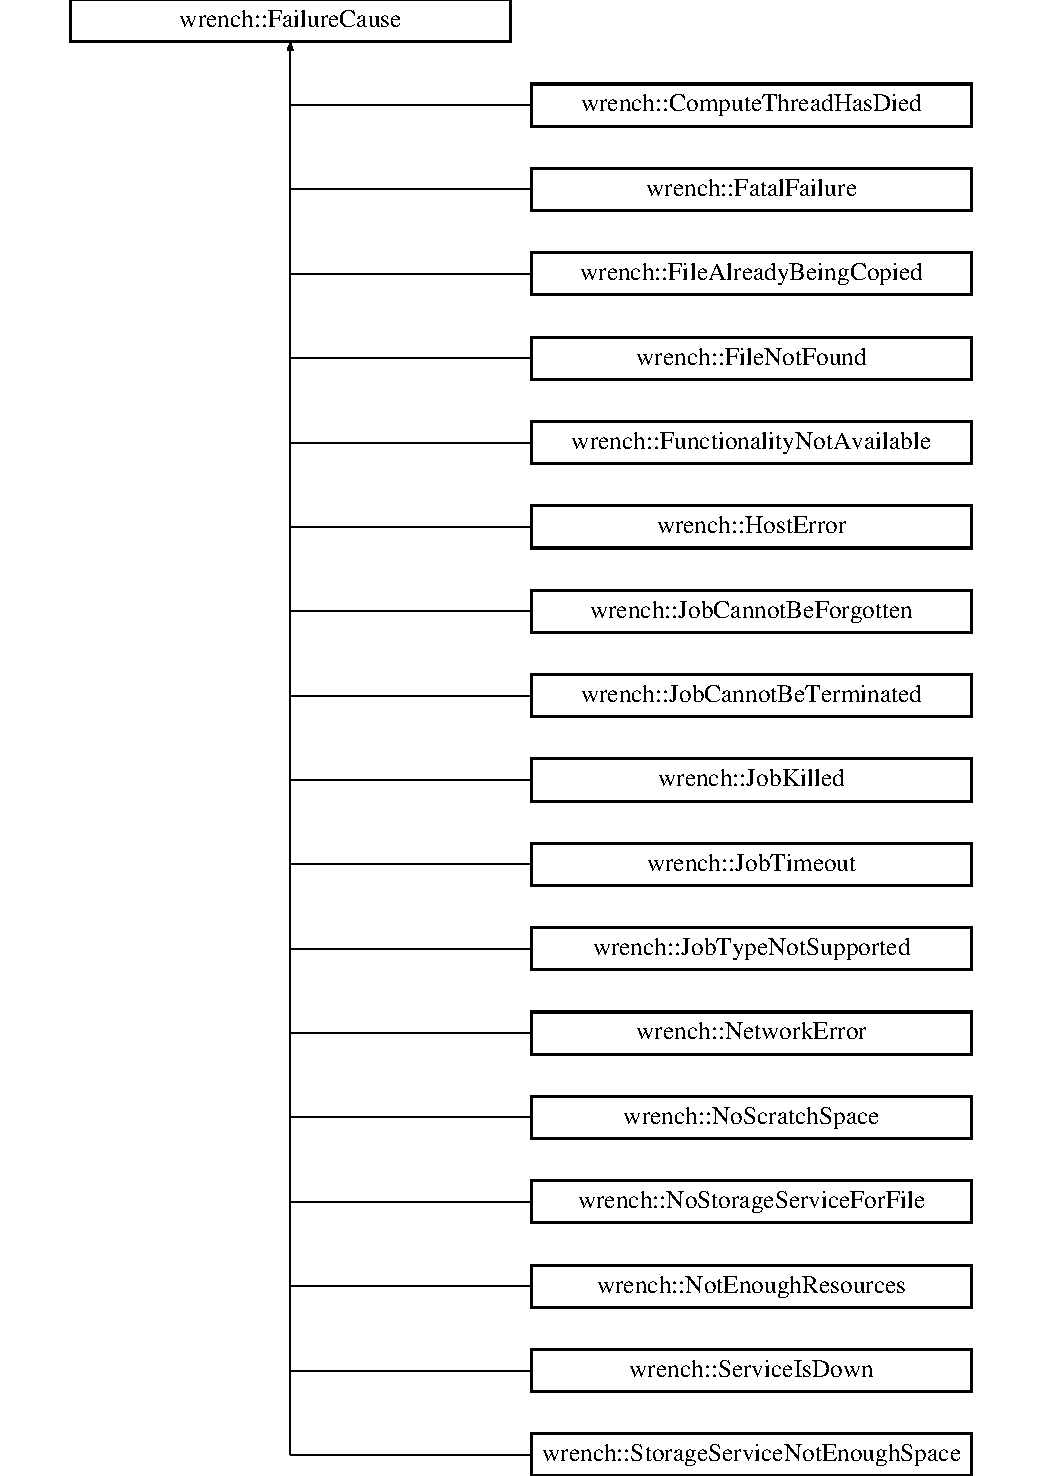
\includegraphics[height=12.000000cm]{classwrench_1_1_failure_cause}
\end{center}
\end{figure}
\subsection*{Public Types}
\begin{DoxyCompactItemize}
\item 
enum \hyperlink{classwrench_1_1_failure_cause_a6d06d6845ca5499c5cbbd9e1a08c9c77}{Cause\+Type} \{ \newline
\hyperlink{classwrench_1_1_failure_cause_a6d06d6845ca5499c5cbbd9e1a08c9c77accf0a8513eb8a8742d7b7f4cf055e05a}{F\+A\+T\+A\+L\+\_\+\+F\+A\+I\+L\+U\+RE}, 
\hyperlink{classwrench_1_1_failure_cause_a6d06d6845ca5499c5cbbd9e1a08c9c77a864646934bad10175377329098b912a6}{N\+O\+\_\+\+S\+T\+O\+R\+A\+G\+E\+\_\+\+S\+E\+R\+V\+I\+C\+E\+\_\+\+F\+O\+R\+\_\+\+F\+I\+LE}, 
\hyperlink{classwrench_1_1_failure_cause_a6d06d6845ca5499c5cbbd9e1a08c9c77a2e0288e55c8d2cf951acf20d4640b469}{N\+O\+\_\+\+S\+C\+R\+A\+T\+C\+H\+\_\+\+S\+P\+A\+CE}, 
\hyperlink{classwrench_1_1_failure_cause_a6d06d6845ca5499c5cbbd9e1a08c9c77ab5690623631a20fbb24bcabfb7806bf2}{F\+I\+L\+E\+\_\+\+N\+O\+T\+\_\+\+F\+O\+U\+ND}, 
\newline
\hyperlink{classwrench_1_1_failure_cause_a6d06d6845ca5499c5cbbd9e1a08c9c77abdc62ab4e21f2909db76e1f503e9c44c}{F\+I\+L\+E\+\_\+\+A\+L\+R\+E\+A\+D\+Y\+\_\+\+T\+H\+E\+RE}, 
\hyperlink{classwrench_1_1_failure_cause_a6d06d6845ca5499c5cbbd9e1a08c9c77a7f78628f013c41cc1ff269614d2e9f5c}{F\+I\+L\+E\+\_\+\+A\+L\+R\+E\+A\+D\+Y\+\_\+\+B\+E\+I\+N\+G\+\_\+\+C\+O\+P\+I\+ED}, 
\hyperlink{classwrench_1_1_failure_cause_a6d06d6845ca5499c5cbbd9e1a08c9c77ab25836e82d005c2f3eb72cdfe247feec}{S\+T\+O\+R\+A\+G\+E\+\_\+\+N\+O\+T\+\_\+\+E\+N\+O\+U\+G\+H\+\_\+\+S\+P\+A\+CE}, 
\hyperlink{classwrench_1_1_failure_cause_a6d06d6845ca5499c5cbbd9e1a08c9c77a89fb949be686938482b82a78297cf90c}{S\+E\+R\+V\+I\+C\+E\+\_\+\+D\+O\+WN}, 
\newline
\hyperlink{classwrench_1_1_failure_cause_a6d06d6845ca5499c5cbbd9e1a08c9c77aff608d63d9d05fc76c44ba7cd39053e6}{J\+O\+B\+\_\+\+T\+Y\+P\+E\+\_\+\+N\+O\+T\+\_\+\+S\+U\+P\+P\+O\+R\+T\+ED}, 
\hyperlink{classwrench_1_1_failure_cause_a6d06d6845ca5499c5cbbd9e1a08c9c77a0b39d227bbca2c1585f2a322fa92d614}{N\+O\+T\+\_\+\+E\+N\+O\+U\+G\+H\+\_\+\+R\+E\+S\+O\+U\+R\+C\+ES}, 
\hyperlink{classwrench_1_1_failure_cause_a6d06d6845ca5499c5cbbd9e1a08c9c77a02d62b0456ff50fd6ad1ebf2f749327d}{N\+E\+T\+W\+O\+R\+K\+\_\+\+E\+R\+R\+OR}, 
\hyperlink{classwrench_1_1_failure_cause_a6d06d6845ca5499c5cbbd9e1a08c9c77a74db928f7b05128dbaf2462588c7208f}{N\+E\+T\+W\+O\+R\+K\+\_\+\+T\+I\+M\+E\+O\+UT}, 
\newline
\hyperlink{classwrench_1_1_failure_cause_a6d06d6845ca5499c5cbbd9e1a08c9c77ae26e9df054dd1df285e7d0ab8f350869}{J\+O\+B\+\_\+\+K\+I\+L\+L\+ED}, 
\hyperlink{classwrench_1_1_failure_cause_a6d06d6845ca5499c5cbbd9e1a08c9c77af3188a3cd262d0ef0e0b985c0f3bc93d}{J\+O\+B\+\_\+\+C\+A\+N\+N\+O\+T\+\_\+\+B\+E\+\_\+\+T\+E\+R\+M\+I\+N\+A\+T\+ED}, 
\hyperlink{classwrench_1_1_failure_cause_a6d06d6845ca5499c5cbbd9e1a08c9c77ae4e51f06537ecc8ab4f7a5b3a890b2a5}{J\+O\+B\+\_\+\+C\+A\+N\+N\+O\+T\+\_\+\+B\+E\+\_\+\+F\+O\+R\+G\+O\+T\+T\+EN}, 
\hyperlink{classwrench_1_1_failure_cause_a6d06d6845ca5499c5cbbd9e1a08c9c77a709b0b9c94851003622d5ec900f186f6}{C\+O\+M\+P\+U\+T\+E\+\_\+\+T\+H\+R\+E\+A\+D\+\_\+\+H\+A\+S\+\_\+\+D\+I\+ED}, 
\newline
\hyperlink{classwrench_1_1_failure_cause_a6d06d6845ca5499c5cbbd9e1a08c9c77a362e54af1fdb80512e4708504105d8c0}{F\+U\+N\+C\+T\+I\+O\+N\+A\+L\+I\+T\+Y\+\_\+\+N\+O\+T\+\_\+\+A\+V\+A\+I\+L\+A\+B\+LE}, 
\hyperlink{classwrench_1_1_failure_cause_a6d06d6845ca5499c5cbbd9e1a08c9c77a60d4bf28e7842c657ebe0c429b32f423}{J\+O\+B\+\_\+\+T\+I\+M\+E\+O\+UT}, 
\hyperlink{classwrench_1_1_failure_cause_a6d06d6845ca5499c5cbbd9e1a08c9c77ac063809cfa1d103f49dd7d25939a54d4}{H\+O\+S\+T\+\_\+\+E\+R\+R\+OR}
 \}\begin{DoxyCompactList}\small\item\em Types of failure causes. \end{DoxyCompactList}
\end{DoxyCompactItemize}
\subsection*{Public Member Functions}
\begin{DoxyCompactItemize}
\item 
\hyperlink{classwrench_1_1_failure_cause_ac18f4c292fbdc1878da7ae2431c7d3e4}{Failure\+Cause} (\hyperlink{classwrench_1_1_failure_cause_a6d06d6845ca5499c5cbbd9e1a08c9c77}{Cause\+Type} cause)
\begin{DoxyCompactList}\small\item\em Constructor. \end{DoxyCompactList}\item 
\hyperlink{classwrench_1_1_failure_cause_a6d06d6845ca5499c5cbbd9e1a08c9c77}{Cause\+Type} \hyperlink{classwrench_1_1_failure_cause_a24fa4deecfa2e5e187f8d88187b8dddb}{get\+Cause\+Type} ()
\begin{DoxyCompactList}\small\item\em Retrieve the type of the failure cause. \end{DoxyCompactList}\item 
virtual std\+::string \hyperlink{classwrench_1_1_failure_cause_afbad248ebe902409f2cd4f1d6f2b867d}{to\+String} ()=0
\begin{DoxyCompactList}\small\item\em Return an error message that describes the failure cause (to be overridden) \end{DoxyCompactList}\end{DoxyCompactItemize}


\subsection{Detailed Description}
A top-\/level class to describe all simulation-\/valid failures that can occur during workflow execution (and should/could be handled by a \hyperlink{classwrench_1_1_w_m_s}{W\+MS}) 

\subsection{Member Enumeration Documentation}
\mbox{\Hypertarget{classwrench_1_1_failure_cause_a6d06d6845ca5499c5cbbd9e1a08c9c77}\label{classwrench_1_1_failure_cause_a6d06d6845ca5499c5cbbd9e1a08c9c77}} 
\index{wrench\+::\+Failure\+Cause@{wrench\+::\+Failure\+Cause}!Cause\+Type@{Cause\+Type}}
\index{Cause\+Type@{Cause\+Type}!wrench\+::\+Failure\+Cause@{wrench\+::\+Failure\+Cause}}
\subsubsection{\texorpdfstring{Cause\+Type}{CauseType}}
{\footnotesize\ttfamily enum \hyperlink{classwrench_1_1_failure_cause_a6d06d6845ca5499c5cbbd9e1a08c9c77}{wrench\+::\+Failure\+Cause\+::\+Cause\+Type}}



Types of failure causes. 

\begin{DoxyEnumFields}{Enumerator}
\raisebox{\heightof{T}}[0pt][0pt]{\index{F\+A\+T\+A\+L\+\_\+\+F\+A\+I\+L\+U\+RE@{F\+A\+T\+A\+L\+\_\+\+F\+A\+I\+L\+U\+RE}!wrench\+::\+Failure\+Cause@{wrench\+::\+Failure\+Cause}}\index{wrench\+::\+Failure\+Cause@{wrench\+::\+Failure\+Cause}!F\+A\+T\+A\+L\+\_\+\+F\+A\+I\+L\+U\+RE@{F\+A\+T\+A\+L\+\_\+\+F\+A\+I\+L\+U\+RE}}}\mbox{\Hypertarget{classwrench_1_1_failure_cause_a6d06d6845ca5499c5cbbd9e1a08c9c77accf0a8513eb8a8742d7b7f4cf055e05a}\label{classwrench_1_1_failure_cause_a6d06d6845ca5499c5cbbd9e1a08c9c77accf0a8513eb8a8742d7b7f4cf055e05a}} 
F\+A\+T\+A\+L\+\_\+\+F\+A\+I\+L\+U\+RE&Unknown cause. \\
\hline

\raisebox{\heightof{T}}[0pt][0pt]{\index{N\+O\+\_\+\+S\+T\+O\+R\+A\+G\+E\+\_\+\+S\+E\+R\+V\+I\+C\+E\+\_\+\+F\+O\+R\+\_\+\+F\+I\+LE@{N\+O\+\_\+\+S\+T\+O\+R\+A\+G\+E\+\_\+\+S\+E\+R\+V\+I\+C\+E\+\_\+\+F\+O\+R\+\_\+\+F\+I\+LE}!wrench\+::\+Failure\+Cause@{wrench\+::\+Failure\+Cause}}\index{wrench\+::\+Failure\+Cause@{wrench\+::\+Failure\+Cause}!N\+O\+\_\+\+S\+T\+O\+R\+A\+G\+E\+\_\+\+S\+E\+R\+V\+I\+C\+E\+\_\+\+F\+O\+R\+\_\+\+F\+I\+LE@{N\+O\+\_\+\+S\+T\+O\+R\+A\+G\+E\+\_\+\+S\+E\+R\+V\+I\+C\+E\+\_\+\+F\+O\+R\+\_\+\+F\+I\+LE}}}\mbox{\Hypertarget{classwrench_1_1_failure_cause_a6d06d6845ca5499c5cbbd9e1a08c9c77a864646934bad10175377329098b912a6}\label{classwrench_1_1_failure_cause_a6d06d6845ca5499c5cbbd9e1a08c9c77a864646934bad10175377329098b912a6}} 
N\+O\+\_\+\+S\+T\+O\+R\+A\+G\+E\+\_\+\+S\+E\+R\+V\+I\+C\+E\+\_\+\+F\+O\+R\+\_\+\+F\+I\+LE&The file cannot be found anywhere. \\
\hline

\raisebox{\heightof{T}}[0pt][0pt]{\index{N\+O\+\_\+\+S\+C\+R\+A\+T\+C\+H\+\_\+\+S\+P\+A\+CE@{N\+O\+\_\+\+S\+C\+R\+A\+T\+C\+H\+\_\+\+S\+P\+A\+CE}!wrench\+::\+Failure\+Cause@{wrench\+::\+Failure\+Cause}}\index{wrench\+::\+Failure\+Cause@{wrench\+::\+Failure\+Cause}!N\+O\+\_\+\+S\+C\+R\+A\+T\+C\+H\+\_\+\+S\+P\+A\+CE@{N\+O\+\_\+\+S\+C\+R\+A\+T\+C\+H\+\_\+\+S\+P\+A\+CE}}}\mbox{\Hypertarget{classwrench_1_1_failure_cause_a6d06d6845ca5499c5cbbd9e1a08c9c77a2e0288e55c8d2cf951acf20d4640b469}\label{classwrench_1_1_failure_cause_a6d06d6845ca5499c5cbbd9e1a08c9c77a2e0288e55c8d2cf951acf20d4640b469}} 
N\+O\+\_\+\+S\+C\+R\+A\+T\+C\+H\+\_\+\+S\+P\+A\+CE&No Scratch Space is available. \\
\hline

\raisebox{\heightof{T}}[0pt][0pt]{\index{F\+I\+L\+E\+\_\+\+N\+O\+T\+\_\+\+F\+O\+U\+ND@{F\+I\+L\+E\+\_\+\+N\+O\+T\+\_\+\+F\+O\+U\+ND}!wrench\+::\+Failure\+Cause@{wrench\+::\+Failure\+Cause}}\index{wrench\+::\+Failure\+Cause@{wrench\+::\+Failure\+Cause}!F\+I\+L\+E\+\_\+\+N\+O\+T\+\_\+\+F\+O\+U\+ND@{F\+I\+L\+E\+\_\+\+N\+O\+T\+\_\+\+F\+O\+U\+ND}}}\mbox{\Hypertarget{classwrench_1_1_failure_cause_a6d06d6845ca5499c5cbbd9e1a08c9c77ab5690623631a20fbb24bcabfb7806bf2}\label{classwrench_1_1_failure_cause_a6d06d6845ca5499c5cbbd9e1a08c9c77ab5690623631a20fbb24bcabfb7806bf2}} 
F\+I\+L\+E\+\_\+\+N\+O\+T\+\_\+\+F\+O\+U\+ND&The file was not found where it was supposed to be found. \\
\hline

\raisebox{\heightof{T}}[0pt][0pt]{\index{F\+I\+L\+E\+\_\+\+A\+L\+R\+E\+A\+D\+Y\+\_\+\+T\+H\+E\+RE@{F\+I\+L\+E\+\_\+\+A\+L\+R\+E\+A\+D\+Y\+\_\+\+T\+H\+E\+RE}!wrench\+::\+Failure\+Cause@{wrench\+::\+Failure\+Cause}}\index{wrench\+::\+Failure\+Cause@{wrench\+::\+Failure\+Cause}!F\+I\+L\+E\+\_\+\+A\+L\+R\+E\+A\+D\+Y\+\_\+\+T\+H\+E\+RE@{F\+I\+L\+E\+\_\+\+A\+L\+R\+E\+A\+D\+Y\+\_\+\+T\+H\+E\+RE}}}\mbox{\Hypertarget{classwrench_1_1_failure_cause_a6d06d6845ca5499c5cbbd9e1a08c9c77abdc62ab4e21f2909db76e1f503e9c44c}\label{classwrench_1_1_failure_cause_a6d06d6845ca5499c5cbbd9e1a08c9c77abdc62ab4e21f2909db76e1f503e9c44c}} 
F\+I\+L\+E\+\_\+\+A\+L\+R\+E\+A\+D\+Y\+\_\+\+T\+H\+E\+RE&The file to be written is already there. \\
\hline

\raisebox{\heightof{T}}[0pt][0pt]{\index{F\+I\+L\+E\+\_\+\+A\+L\+R\+E\+A\+D\+Y\+\_\+\+B\+E\+I\+N\+G\+\_\+\+C\+O\+P\+I\+ED@{F\+I\+L\+E\+\_\+\+A\+L\+R\+E\+A\+D\+Y\+\_\+\+B\+E\+I\+N\+G\+\_\+\+C\+O\+P\+I\+ED}!wrench\+::\+Failure\+Cause@{wrench\+::\+Failure\+Cause}}\index{wrench\+::\+Failure\+Cause@{wrench\+::\+Failure\+Cause}!F\+I\+L\+E\+\_\+\+A\+L\+R\+E\+A\+D\+Y\+\_\+\+B\+E\+I\+N\+G\+\_\+\+C\+O\+P\+I\+ED@{F\+I\+L\+E\+\_\+\+A\+L\+R\+E\+A\+D\+Y\+\_\+\+B\+E\+I\+N\+G\+\_\+\+C\+O\+P\+I\+ED}}}\mbox{\Hypertarget{classwrench_1_1_failure_cause_a6d06d6845ca5499c5cbbd9e1a08c9c77a7f78628f013c41cc1ff269614d2e9f5c}\label{classwrench_1_1_failure_cause_a6d06d6845ca5499c5cbbd9e1a08c9c77a7f78628f013c41cc1ff269614d2e9f5c}} 
F\+I\+L\+E\+\_\+\+A\+L\+R\+E\+A\+D\+Y\+\_\+\+B\+E\+I\+N\+G\+\_\+\+C\+O\+P\+I\+ED&The file is already being copied there. \\
\hline

\raisebox{\heightof{T}}[0pt][0pt]{\index{S\+T\+O\+R\+A\+G\+E\+\_\+\+N\+O\+T\+\_\+\+E\+N\+O\+U\+G\+H\+\_\+\+S\+P\+A\+CE@{S\+T\+O\+R\+A\+G\+E\+\_\+\+N\+O\+T\+\_\+\+E\+N\+O\+U\+G\+H\+\_\+\+S\+P\+A\+CE}!wrench\+::\+Failure\+Cause@{wrench\+::\+Failure\+Cause}}\index{wrench\+::\+Failure\+Cause@{wrench\+::\+Failure\+Cause}!S\+T\+O\+R\+A\+G\+E\+\_\+\+N\+O\+T\+\_\+\+E\+N\+O\+U\+G\+H\+\_\+\+S\+P\+A\+CE@{S\+T\+O\+R\+A\+G\+E\+\_\+\+N\+O\+T\+\_\+\+E\+N\+O\+U\+G\+H\+\_\+\+S\+P\+A\+CE}}}\mbox{\Hypertarget{classwrench_1_1_failure_cause_a6d06d6845ca5499c5cbbd9e1a08c9c77ab25836e82d005c2f3eb72cdfe247feec}\label{classwrench_1_1_failure_cause_a6d06d6845ca5499c5cbbd9e1a08c9c77ab25836e82d005c2f3eb72cdfe247feec}} 
S\+T\+O\+R\+A\+G\+E\+\_\+\+N\+O\+T\+\_\+\+E\+N\+O\+U\+G\+H\+\_\+\+S\+P\+A\+CE&The storage service does not have enough space to support the requested operation. \\
\hline

\raisebox{\heightof{T}}[0pt][0pt]{\index{S\+E\+R\+V\+I\+C\+E\+\_\+\+D\+O\+WN@{S\+E\+R\+V\+I\+C\+E\+\_\+\+D\+O\+WN}!wrench\+::\+Failure\+Cause@{wrench\+::\+Failure\+Cause}}\index{wrench\+::\+Failure\+Cause@{wrench\+::\+Failure\+Cause}!S\+E\+R\+V\+I\+C\+E\+\_\+\+D\+O\+WN@{S\+E\+R\+V\+I\+C\+E\+\_\+\+D\+O\+WN}}}\mbox{\Hypertarget{classwrench_1_1_failure_cause_a6d06d6845ca5499c5cbbd9e1a08c9c77a89fb949be686938482b82a78297cf90c}\label{classwrench_1_1_failure_cause_a6d06d6845ca5499c5cbbd9e1a08c9c77a89fb949be686938482b82a78297cf90c}} 
S\+E\+R\+V\+I\+C\+E\+\_\+\+D\+O\+WN&The service cannot be used because it is down (likely it was terminated) \\
\hline

\raisebox{\heightof{T}}[0pt][0pt]{\index{J\+O\+B\+\_\+\+T\+Y\+P\+E\+\_\+\+N\+O\+T\+\_\+\+S\+U\+P\+P\+O\+R\+T\+ED@{J\+O\+B\+\_\+\+T\+Y\+P\+E\+\_\+\+N\+O\+T\+\_\+\+S\+U\+P\+P\+O\+R\+T\+ED}!wrench\+::\+Failure\+Cause@{wrench\+::\+Failure\+Cause}}\index{wrench\+::\+Failure\+Cause@{wrench\+::\+Failure\+Cause}!J\+O\+B\+\_\+\+T\+Y\+P\+E\+\_\+\+N\+O\+T\+\_\+\+S\+U\+P\+P\+O\+R\+T\+ED@{J\+O\+B\+\_\+\+T\+Y\+P\+E\+\_\+\+N\+O\+T\+\_\+\+S\+U\+P\+P\+O\+R\+T\+ED}}}\mbox{\Hypertarget{classwrench_1_1_failure_cause_a6d06d6845ca5499c5cbbd9e1a08c9c77aff608d63d9d05fc76c44ba7cd39053e6}\label{classwrench_1_1_failure_cause_a6d06d6845ca5499c5cbbd9e1a08c9c77aff608d63d9d05fc76c44ba7cd39053e6}} 
J\+O\+B\+\_\+\+T\+Y\+P\+E\+\_\+\+N\+O\+T\+\_\+\+S\+U\+P\+P\+O\+R\+T\+ED&The compute service does not support this job type. \\
\hline

\raisebox{\heightof{T}}[0pt][0pt]{\index{N\+O\+T\+\_\+\+E\+N\+O\+U\+G\+H\+\_\+\+R\+E\+S\+O\+U\+R\+C\+ES@{N\+O\+T\+\_\+\+E\+N\+O\+U\+G\+H\+\_\+\+R\+E\+S\+O\+U\+R\+C\+ES}!wrench\+::\+Failure\+Cause@{wrench\+::\+Failure\+Cause}}\index{wrench\+::\+Failure\+Cause@{wrench\+::\+Failure\+Cause}!N\+O\+T\+\_\+\+E\+N\+O\+U\+G\+H\+\_\+\+R\+E\+S\+O\+U\+R\+C\+ES@{N\+O\+T\+\_\+\+E\+N\+O\+U\+G\+H\+\_\+\+R\+E\+S\+O\+U\+R\+C\+ES}}}\mbox{\Hypertarget{classwrench_1_1_failure_cause_a6d06d6845ca5499c5cbbd9e1a08c9c77a0b39d227bbca2c1585f2a322fa92d614}\label{classwrench_1_1_failure_cause_a6d06d6845ca5499c5cbbd9e1a08c9c77a0b39d227bbca2c1585f2a322fa92d614}} 
N\+O\+T\+\_\+\+E\+N\+O\+U\+G\+H\+\_\+\+R\+E\+S\+O\+U\+R\+C\+ES&The compute service cannot run the job (ever) due to insufficient resources (cores and/or ram) \\
\hline

\raisebox{\heightof{T}}[0pt][0pt]{\index{N\+E\+T\+W\+O\+R\+K\+\_\+\+E\+R\+R\+OR@{N\+E\+T\+W\+O\+R\+K\+\_\+\+E\+R\+R\+OR}!wrench\+::\+Failure\+Cause@{wrench\+::\+Failure\+Cause}}\index{wrench\+::\+Failure\+Cause@{wrench\+::\+Failure\+Cause}!N\+E\+T\+W\+O\+R\+K\+\_\+\+E\+R\+R\+OR@{N\+E\+T\+W\+O\+R\+K\+\_\+\+E\+R\+R\+OR}}}\mbox{\Hypertarget{classwrench_1_1_failure_cause_a6d06d6845ca5499c5cbbd9e1a08c9c77a02d62b0456ff50fd6ad1ebf2f749327d}\label{classwrench_1_1_failure_cause_a6d06d6845ca5499c5cbbd9e1a08c9c77a02d62b0456ff50fd6ad1ebf2f749327d}} 
N\+E\+T\+W\+O\+R\+K\+\_\+\+E\+R\+R\+OR&There was a network error, or an endpoint was down. \\
\hline

\raisebox{\heightof{T}}[0pt][0pt]{\index{N\+E\+T\+W\+O\+R\+K\+\_\+\+T\+I\+M\+E\+O\+UT@{N\+E\+T\+W\+O\+R\+K\+\_\+\+T\+I\+M\+E\+O\+UT}!wrench\+::\+Failure\+Cause@{wrench\+::\+Failure\+Cause}}\index{wrench\+::\+Failure\+Cause@{wrench\+::\+Failure\+Cause}!N\+E\+T\+W\+O\+R\+K\+\_\+\+T\+I\+M\+E\+O\+UT@{N\+E\+T\+W\+O\+R\+K\+\_\+\+T\+I\+M\+E\+O\+UT}}}\mbox{\Hypertarget{classwrench_1_1_failure_cause_a6d06d6845ca5499c5cbbd9e1a08c9c77a74db928f7b05128dbaf2462588c7208f}\label{classwrench_1_1_failure_cause_a6d06d6845ca5499c5cbbd9e1a08c9c77a74db928f7b05128dbaf2462588c7208f}} 
N\+E\+T\+W\+O\+R\+K\+\_\+\+T\+I\+M\+E\+O\+UT&There was a network timeout (for a \char`\"{}with timeout\char`\"{} network operation) \\
\hline

\raisebox{\heightof{T}}[0pt][0pt]{\index{J\+O\+B\+\_\+\+K\+I\+L\+L\+ED@{J\+O\+B\+\_\+\+K\+I\+L\+L\+ED}!wrench\+::\+Failure\+Cause@{wrench\+::\+Failure\+Cause}}\index{wrench\+::\+Failure\+Cause@{wrench\+::\+Failure\+Cause}!J\+O\+B\+\_\+\+K\+I\+L\+L\+ED@{J\+O\+B\+\_\+\+K\+I\+L\+L\+ED}}}\mbox{\Hypertarget{classwrench_1_1_failure_cause_a6d06d6845ca5499c5cbbd9e1a08c9c77ae26e9df054dd1df285e7d0ab8f350869}\label{classwrench_1_1_failure_cause_a6d06d6845ca5499c5cbbd9e1a08c9c77ae26e9df054dd1df285e7d0ab8f350869}} 
J\+O\+B\+\_\+\+K\+I\+L\+L\+ED&A Job has been killed (likely because the service performing it was terminated) \\
\hline

\raisebox{\heightof{T}}[0pt][0pt]{\index{J\+O\+B\+\_\+\+C\+A\+N\+N\+O\+T\+\_\+\+B\+E\+\_\+\+T\+E\+R\+M\+I\+N\+A\+T\+ED@{J\+O\+B\+\_\+\+C\+A\+N\+N\+O\+T\+\_\+\+B\+E\+\_\+\+T\+E\+R\+M\+I\+N\+A\+T\+ED}!wrench\+::\+Failure\+Cause@{wrench\+::\+Failure\+Cause}}\index{wrench\+::\+Failure\+Cause@{wrench\+::\+Failure\+Cause}!J\+O\+B\+\_\+\+C\+A\+N\+N\+O\+T\+\_\+\+B\+E\+\_\+\+T\+E\+R\+M\+I\+N\+A\+T\+ED@{J\+O\+B\+\_\+\+C\+A\+N\+N\+O\+T\+\_\+\+B\+E\+\_\+\+T\+E\+R\+M\+I\+N\+A\+T\+ED}}}\mbox{\Hypertarget{classwrench_1_1_failure_cause_a6d06d6845ca5499c5cbbd9e1a08c9c77af3188a3cd262d0ef0e0b985c0f3bc93d}\label{classwrench_1_1_failure_cause_a6d06d6845ca5499c5cbbd9e1a08c9c77af3188a3cd262d0ef0e0b985c0f3bc93d}} 
J\+O\+B\+\_\+\+C\+A\+N\+N\+O\+T\+\_\+\+B\+E\+\_\+\+T\+E\+R\+M\+I\+N\+A\+T\+ED&The job cannot be terminated because it is neither pending nor running. \\
\hline

\raisebox{\heightof{T}}[0pt][0pt]{\index{J\+O\+B\+\_\+\+C\+A\+N\+N\+O\+T\+\_\+\+B\+E\+\_\+\+F\+O\+R\+G\+O\+T\+T\+EN@{J\+O\+B\+\_\+\+C\+A\+N\+N\+O\+T\+\_\+\+B\+E\+\_\+\+F\+O\+R\+G\+O\+T\+T\+EN}!wrench\+::\+Failure\+Cause@{wrench\+::\+Failure\+Cause}}\index{wrench\+::\+Failure\+Cause@{wrench\+::\+Failure\+Cause}!J\+O\+B\+\_\+\+C\+A\+N\+N\+O\+T\+\_\+\+B\+E\+\_\+\+F\+O\+R\+G\+O\+T\+T\+EN@{J\+O\+B\+\_\+\+C\+A\+N\+N\+O\+T\+\_\+\+B\+E\+\_\+\+F\+O\+R\+G\+O\+T\+T\+EN}}}\mbox{\Hypertarget{classwrench_1_1_failure_cause_a6d06d6845ca5499c5cbbd9e1a08c9c77ae4e51f06537ecc8ab4f7a5b3a890b2a5}\label{classwrench_1_1_failure_cause_a6d06d6845ca5499c5cbbd9e1a08c9c77ae4e51f06537ecc8ab4f7a5b3a890b2a5}} 
J\+O\+B\+\_\+\+C\+A\+N\+N\+O\+T\+\_\+\+B\+E\+\_\+\+F\+O\+R\+G\+O\+T\+T\+EN&The job cannot be forgotten because it is not completed. \\
\hline

\raisebox{\heightof{T}}[0pt][0pt]{\index{C\+O\+M\+P\+U\+T\+E\+\_\+\+T\+H\+R\+E\+A\+D\+\_\+\+H\+A\+S\+\_\+\+D\+I\+ED@{C\+O\+M\+P\+U\+T\+E\+\_\+\+T\+H\+R\+E\+A\+D\+\_\+\+H\+A\+S\+\_\+\+D\+I\+ED}!wrench\+::\+Failure\+Cause@{wrench\+::\+Failure\+Cause}}\index{wrench\+::\+Failure\+Cause@{wrench\+::\+Failure\+Cause}!C\+O\+M\+P\+U\+T\+E\+\_\+\+T\+H\+R\+E\+A\+D\+\_\+\+H\+A\+S\+\_\+\+D\+I\+ED@{C\+O\+M\+P\+U\+T\+E\+\_\+\+T\+H\+R\+E\+A\+D\+\_\+\+H\+A\+S\+\_\+\+D\+I\+ED}}}\mbox{\Hypertarget{classwrench_1_1_failure_cause_a6d06d6845ca5499c5cbbd9e1a08c9c77a709b0b9c94851003622d5ec900f186f6}\label{classwrench_1_1_failure_cause_a6d06d6845ca5499c5cbbd9e1a08c9c77a709b0b9c94851003622d5ec900f186f6}} 
C\+O\+M\+P\+U\+T\+E\+\_\+\+T\+H\+R\+E\+A\+D\+\_\+\+H\+A\+S\+\_\+\+D\+I\+ED&A compute thread has died. \\
\hline

\raisebox{\heightof{T}}[0pt][0pt]{\index{F\+U\+N\+C\+T\+I\+O\+N\+A\+L\+I\+T\+Y\+\_\+\+N\+O\+T\+\_\+\+A\+V\+A\+I\+L\+A\+B\+LE@{F\+U\+N\+C\+T\+I\+O\+N\+A\+L\+I\+T\+Y\+\_\+\+N\+O\+T\+\_\+\+A\+V\+A\+I\+L\+A\+B\+LE}!wrench\+::\+Failure\+Cause@{wrench\+::\+Failure\+Cause}}\index{wrench\+::\+Failure\+Cause@{wrench\+::\+Failure\+Cause}!F\+U\+N\+C\+T\+I\+O\+N\+A\+L\+I\+T\+Y\+\_\+\+N\+O\+T\+\_\+\+A\+V\+A\+I\+L\+A\+B\+LE@{F\+U\+N\+C\+T\+I\+O\+N\+A\+L\+I\+T\+Y\+\_\+\+N\+O\+T\+\_\+\+A\+V\+A\+I\+L\+A\+B\+LE}}}\mbox{\Hypertarget{classwrench_1_1_failure_cause_a6d06d6845ca5499c5cbbd9e1a08c9c77a362e54af1fdb80512e4708504105d8c0}\label{classwrench_1_1_failure_cause_a6d06d6845ca5499c5cbbd9e1a08c9c77a362e54af1fdb80512e4708504105d8c0}} 
F\+U\+N\+C\+T\+I\+O\+N\+A\+L\+I\+T\+Y\+\_\+\+N\+O\+T\+\_\+\+A\+V\+A\+I\+L\+A\+B\+LE&A functionality is not available. \\
\hline

\raisebox{\heightof{T}}[0pt][0pt]{\index{J\+O\+B\+\_\+\+T\+I\+M\+E\+O\+UT@{J\+O\+B\+\_\+\+T\+I\+M\+E\+O\+UT}!wrench\+::\+Failure\+Cause@{wrench\+::\+Failure\+Cause}}\index{wrench\+::\+Failure\+Cause@{wrench\+::\+Failure\+Cause}!J\+O\+B\+\_\+\+T\+I\+M\+E\+O\+UT@{J\+O\+B\+\_\+\+T\+I\+M\+E\+O\+UT}}}\mbox{\Hypertarget{classwrench_1_1_failure_cause_a6d06d6845ca5499c5cbbd9e1a08c9c77a60d4bf28e7842c657ebe0c429b32f423}\label{classwrench_1_1_failure_cause_a6d06d6845ca5499c5cbbd9e1a08c9c77a60d4bf28e7842c657ebe0c429b32f423}} 
J\+O\+B\+\_\+\+T\+I\+M\+E\+O\+UT&A job was terminated due to a timeout. \\
\hline

\raisebox{\heightof{T}}[0pt][0pt]{\index{H\+O\+S\+T\+\_\+\+E\+R\+R\+OR@{H\+O\+S\+T\+\_\+\+E\+R\+R\+OR}!wrench\+::\+Failure\+Cause@{wrench\+::\+Failure\+Cause}}\index{wrench\+::\+Failure\+Cause@{wrench\+::\+Failure\+Cause}!H\+O\+S\+T\+\_\+\+E\+R\+R\+OR@{H\+O\+S\+T\+\_\+\+E\+R\+R\+OR}}}\mbox{\Hypertarget{classwrench_1_1_failure_cause_a6d06d6845ca5499c5cbbd9e1a08c9c77ac063809cfa1d103f49dd7d25939a54d4}\label{classwrench_1_1_failure_cause_a6d06d6845ca5499c5cbbd9e1a08c9c77ac063809cfa1d103f49dd7d25939a54d4}} 
H\+O\+S\+T\+\_\+\+E\+R\+R\+OR&The host went down (while computing, while sleeping) \\
\hline

\end{DoxyEnumFields}


\subsection{Constructor \& Destructor Documentation}
\mbox{\Hypertarget{classwrench_1_1_failure_cause_ac18f4c292fbdc1878da7ae2431c7d3e4}\label{classwrench_1_1_failure_cause_ac18f4c292fbdc1878da7ae2431c7d3e4}} 
\index{wrench\+::\+Failure\+Cause@{wrench\+::\+Failure\+Cause}!Failure\+Cause@{Failure\+Cause}}
\index{Failure\+Cause@{Failure\+Cause}!wrench\+::\+Failure\+Cause@{wrench\+::\+Failure\+Cause}}
\subsubsection{\texorpdfstring{Failure\+Cause()}{FailureCause()}}
{\footnotesize\ttfamily wrench\+::\+Failure\+Cause\+::\+Failure\+Cause (\begin{DoxyParamCaption}\item[{\hyperlink{classwrench_1_1_failure_cause_a6d06d6845ca5499c5cbbd9e1a08c9c77}{Cause\+Type}}]{cause }\end{DoxyParamCaption})\hspace{0.3cm}{\ttfamily [explicit]}}



Constructor. 


\begin{DoxyParams}{Parameters}
{\em cause} & the type of the failure cause \\
\hline
\end{DoxyParams}


\subsection{Member Function Documentation}
\mbox{\Hypertarget{classwrench_1_1_failure_cause_a24fa4deecfa2e5e187f8d88187b8dddb}\label{classwrench_1_1_failure_cause_a24fa4deecfa2e5e187f8d88187b8dddb}} 
\index{wrench\+::\+Failure\+Cause@{wrench\+::\+Failure\+Cause}!get\+Cause\+Type@{get\+Cause\+Type}}
\index{get\+Cause\+Type@{get\+Cause\+Type}!wrench\+::\+Failure\+Cause@{wrench\+::\+Failure\+Cause}}
\subsubsection{\texorpdfstring{get\+Cause\+Type()}{getCauseType()}}
{\footnotesize\ttfamily \hyperlink{classwrench_1_1_failure_cause_a6d06d6845ca5499c5cbbd9e1a08c9c77}{Failure\+Cause\+::\+Cause\+Type} wrench\+::\+Failure\+Cause\+::get\+Cause\+Type (\begin{DoxyParamCaption}{ }\end{DoxyParamCaption})}



Retrieve the type of the failure cause. 

\begin{DoxyReturn}{Returns}

\end{DoxyReturn}
\mbox{\Hypertarget{classwrench_1_1_failure_cause_afbad248ebe902409f2cd4f1d6f2b867d}\label{classwrench_1_1_failure_cause_afbad248ebe902409f2cd4f1d6f2b867d}} 
\index{wrench\+::\+Failure\+Cause@{wrench\+::\+Failure\+Cause}!to\+String@{to\+String}}
\index{to\+String@{to\+String}!wrench\+::\+Failure\+Cause@{wrench\+::\+Failure\+Cause}}
\subsubsection{\texorpdfstring{to\+String()}{toString()}}
{\footnotesize\ttfamily virtual std\+::string wrench\+::\+Failure\+Cause\+::to\+String (\begin{DoxyParamCaption}{ }\end{DoxyParamCaption})\hspace{0.3cm}{\ttfamily [pure virtual]}}



Return an error message that describes the failure cause (to be overridden) 

\begin{DoxyReturn}{Returns}
an error message 
\end{DoxyReturn}


Implemented in \hyperlink{classwrench_1_1_job_timeout_a91515ca59f71777de74a4b0b169d12e7}{wrench\+::\+Job\+Timeout}, \hyperlink{classwrench_1_1_fatal_failure_a4b547da3bac56b7b23aeba34c2dbbd39}{wrench\+::\+Fatal\+Failure}, \hyperlink{classwrench_1_1_compute_thread_has_died_a4725416d9ff31b39ec9d48d23d1c1c0b}{wrench\+::\+Compute\+Thread\+Has\+Died}, \hyperlink{classwrench_1_1_job_cannot_be_forgotten_abbfbece144c738c9948bf8f01d6bbd53}{wrench\+::\+Job\+Cannot\+Be\+Forgotten}, \hyperlink{classwrench_1_1_job_cannot_be_terminated_acfa2b83db93bb68e0e773cc8b4a45505}{wrench\+::\+Job\+Cannot\+Be\+Terminated}, \hyperlink{classwrench_1_1_host_error_adacb96198ee8477b67fcac9ff8638266}{wrench\+::\+Host\+Error}, \hyperlink{classwrench_1_1_network_error_a114346c3faa84b3925600e9a22314a37}{wrench\+::\+Network\+Error}, \hyperlink{classwrench_1_1_job_killed_aa9c6b749d16db4a313ffdd83629f1c76}{wrench\+::\+Job\+Killed}, \hyperlink{classwrench_1_1_not_enough_resources_aeccad36aeccb259ac4c2d17752963269}{wrench\+::\+Not\+Enough\+Resources}, \hyperlink{classwrench_1_1_functionality_not_available_af19ea11f7e3d50d0bea7c8a66b7b1221}{wrench\+::\+Functionality\+Not\+Available}, \hyperlink{classwrench_1_1_job_type_not_supported_ab6a302367f2db332484da0c256e3ae5c}{wrench\+::\+Job\+Type\+Not\+Supported}, \hyperlink{classwrench_1_1_service_is_down_a29dbb2d3dd1b5d6a47536bab974b7151}{wrench\+::\+Service\+Is\+Down}, \hyperlink{classwrench_1_1_file_already_being_copied_a44fa6078be3bd9e0b06cd536b691666c}{wrench\+::\+File\+Already\+Being\+Copied}, \hyperlink{classwrench_1_1_storage_service_not_enough_space_a42680e32c21db44888e173d6a0358326}{wrench\+::\+Storage\+Service\+Not\+Enough\+Space}, \hyperlink{classwrench_1_1_file_not_found_ac9c3bdcc58b4626a0f3de0b4288bf4b4}{wrench\+::\+File\+Not\+Found}, \hyperlink{classwrench_1_1_no_scratch_space_add628f91104786a99a410ec07abac54c}{wrench\+::\+No\+Scratch\+Space}, and \hyperlink{classwrench_1_1_no_storage_service_for_file_ab3941ca284f35abd00e9292e22d7d553}{wrench\+::\+No\+Storage\+Service\+For\+File}.



The documentation for this class was generated from the following files\+:\begin{DoxyCompactItemize}
\item 
/\+Users/rafsilva/\+Documents/isi/workspace/wrench/wrench/include/wrench/workflow/execution\+\_\+events/Failure\+Cause.\+h\item 
/\+Users/rafsilva/\+Documents/isi/workspace/wrench/wrench/src/wrench/workflow/execution\+\_\+events/Failure\+Cause.\+cpp\end{DoxyCompactItemize}

\hypertarget{classwrench_1_1_fatal_failure}{}\section{wrench\+:\+:Fatal\+Failure Class Reference}
\label{classwrench_1_1_fatal_failure}\index{wrench\+::\+Fatal\+Failure@{wrench\+::\+Fatal\+Failure}}


An \char`\"{}\+Unknown\char`\"{} failure cause (should not happen)  




{\ttfamily \#include $<$Failure\+Cause.\+h$>$}

Inheritance diagram for wrench\+:\+:Fatal\+Failure\+:\begin{figure}[H]
\begin{center}
\leavevmode
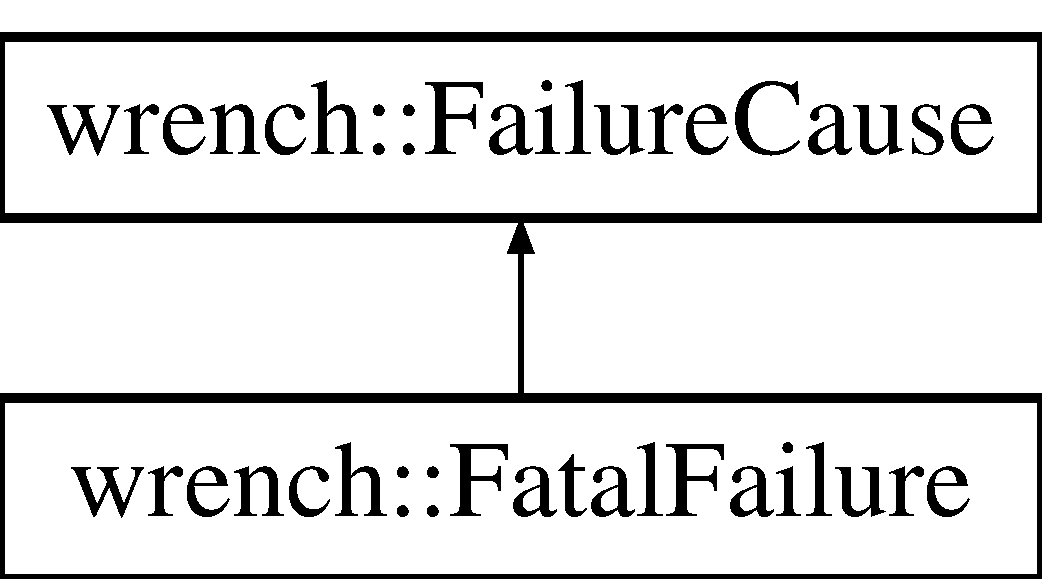
\includegraphics[height=2.000000cm]{classwrench_1_1_fatal_failure}
\end{center}
\end{figure}
\subsection*{Public Member Functions}
\begin{DoxyCompactItemize}
\item 
\mbox{\Hypertarget{classwrench_1_1_fatal_failure_af926761acc0458ebbb315d23f83e0d50}\label{classwrench_1_1_fatal_failure_af926761acc0458ebbb315d23f83e0d50}} 
\hyperlink{classwrench_1_1_fatal_failure_af926761acc0458ebbb315d23f83e0d50}{Fatal\+Failure} ()
\begin{DoxyCompactList}\small\item\em Constructor. \end{DoxyCompactList}\item 
std\+::string \hyperlink{classwrench_1_1_fatal_failure_a4b547da3bac56b7b23aeba34c2dbbd39}{to\+String} ()
\begin{DoxyCompactList}\small\item\em Get the human-\/readable failure message. \end{DoxyCompactList}\end{DoxyCompactItemize}
\subsection*{Additional Inherited Members}


\subsection{Detailed Description}
An \char`\"{}\+Unknown\char`\"{} failure cause (should not happen) 

\subsection{Member Function Documentation}
\mbox{\Hypertarget{classwrench_1_1_fatal_failure_a4b547da3bac56b7b23aeba34c2dbbd39}\label{classwrench_1_1_fatal_failure_a4b547da3bac56b7b23aeba34c2dbbd39}} 
\index{wrench\+::\+Fatal\+Failure@{wrench\+::\+Fatal\+Failure}!to\+String@{to\+String}}
\index{to\+String@{to\+String}!wrench\+::\+Fatal\+Failure@{wrench\+::\+Fatal\+Failure}}
\subsubsection{\texorpdfstring{to\+String()}{toString()}}
{\footnotesize\ttfamily std\+::string wrench\+::\+Fatal\+Failure\+::to\+String (\begin{DoxyParamCaption}{ }\end{DoxyParamCaption})\hspace{0.3cm}{\ttfamily [virtual]}}



Get the human-\/readable failure message. 

\begin{DoxyReturn}{Returns}
the message 
\end{DoxyReturn}


Implements \hyperlink{classwrench_1_1_failure_cause_afbad248ebe902409f2cd4f1d6f2b867d}{wrench\+::\+Failure\+Cause}.



The documentation for this class was generated from the following files\+:\begin{DoxyCompactItemize}
\item 
/\+Users/rafsilva/\+Documents/isi/workspace/wrench/wrench/include/wrench/workflow/execution\+\_\+events/Failure\+Cause.\+h\item 
/\+Users/rafsilva/\+Documents/isi/workspace/wrench/wrench/src/wrench/workflow/execution\+\_\+events/Failure\+Cause.\+cpp\end{DoxyCompactItemize}

\hypertarget{classwrench_1_1_file_already_being_copied}{}\section{wrench\+:\+:File\+Already\+Being\+Copied Class Reference}
\label{classwrench_1_1_file_already_being_copied}\index{wrench\+::\+File\+Already\+Being\+Copied@{wrench\+::\+File\+Already\+Being\+Copied}}


A \char`\"{}file is already there\char`\"{} failure cause.  




{\ttfamily \#include $<$Failure\+Cause.\+h$>$}

Inheritance diagram for wrench\+:\+:File\+Already\+Being\+Copied\+:\begin{figure}[H]
\begin{center}
\leavevmode
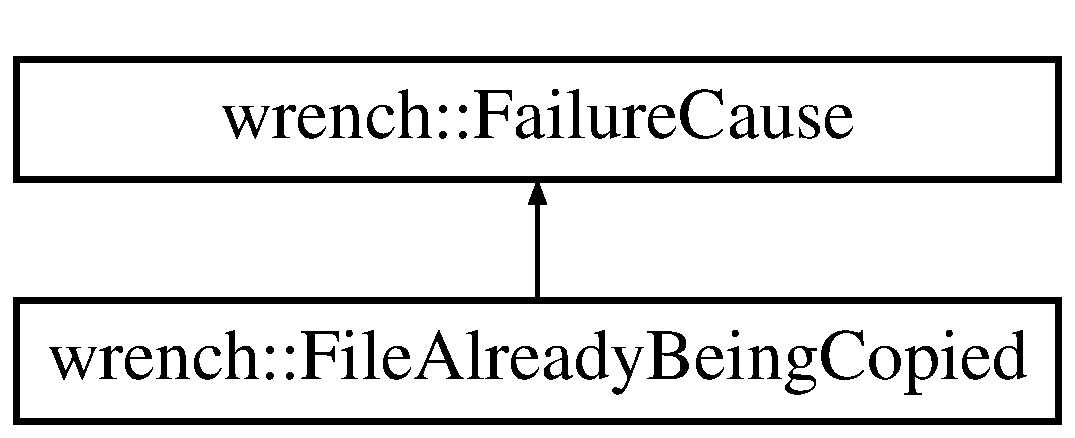
\includegraphics[height=2.000000cm]{classwrench_1_1_file_already_being_copied}
\end{center}
\end{figure}
\subsection*{Public Member Functions}
\begin{DoxyCompactItemize}
\item 
\hyperlink{classwrench_1_1_workflow_file}{Workflow\+File} $\ast$ \hyperlink{classwrench_1_1_file_already_being_copied_a4bb8bd28c57ad1c9a37985b45f5005f4}{get\+File} ()
\begin{DoxyCompactList}\small\item\em Getter. \end{DoxyCompactList}\item 
std\+::string \hyperlink{classwrench_1_1_file_already_being_copied_af1e681d40a77ced81ce05fa49f1fabf5}{get\+Partition} ()
\begin{DoxyCompactList}\small\item\em Getter. \end{DoxyCompactList}\item 
\hyperlink{classwrench_1_1_storage_service}{Storage\+Service} $\ast$ \hyperlink{classwrench_1_1_file_already_being_copied_afac6f9f7f7dae1f51487c5a6223cad30}{get\+Storage\+Service} ()
\begin{DoxyCompactList}\small\item\em Getter. \end{DoxyCompactList}\item 
std\+::string \hyperlink{classwrench_1_1_file_already_being_copied_a44fa6078be3bd9e0b06cd536b691666c}{to\+String} ()
\begin{DoxyCompactList}\small\item\em Get the human-\/readable failure message. \end{DoxyCompactList}\end{DoxyCompactItemize}
\subsection*{Additional Inherited Members}


\subsection{Detailed Description}
A \char`\"{}file is already there\char`\"{} failure cause. 

/$\ast$$\ast$ A \char`\"{}file is already being copied\char`\"{} failure cause 

\subsection{Member Function Documentation}
\mbox{\Hypertarget{classwrench_1_1_file_already_being_copied_a4bb8bd28c57ad1c9a37985b45f5005f4}\label{classwrench_1_1_file_already_being_copied_a4bb8bd28c57ad1c9a37985b45f5005f4}} 
\index{wrench\+::\+File\+Already\+Being\+Copied@{wrench\+::\+File\+Already\+Being\+Copied}!get\+File@{get\+File}}
\index{get\+File@{get\+File}!wrench\+::\+File\+Already\+Being\+Copied@{wrench\+::\+File\+Already\+Being\+Copied}}
\subsubsection{\texorpdfstring{get\+File()}{getFile()}}
{\footnotesize\ttfamily \hyperlink{classwrench_1_1_workflow_file}{Workflow\+File} $\ast$ wrench\+::\+File\+Already\+Being\+Copied\+::get\+File (\begin{DoxyParamCaption}{ }\end{DoxyParamCaption})}



Getter. 

\begin{DoxyReturn}{Returns}
the file 
\end{DoxyReturn}
\mbox{\Hypertarget{classwrench_1_1_file_already_being_copied_af1e681d40a77ced81ce05fa49f1fabf5}\label{classwrench_1_1_file_already_being_copied_af1e681d40a77ced81ce05fa49f1fabf5}} 
\index{wrench\+::\+File\+Already\+Being\+Copied@{wrench\+::\+File\+Already\+Being\+Copied}!get\+Partition@{get\+Partition}}
\index{get\+Partition@{get\+Partition}!wrench\+::\+File\+Already\+Being\+Copied@{wrench\+::\+File\+Already\+Being\+Copied}}
\subsubsection{\texorpdfstring{get\+Partition()}{getPartition()}}
{\footnotesize\ttfamily std\+::string wrench\+::\+File\+Already\+Being\+Copied\+::get\+Partition (\begin{DoxyParamCaption}{ }\end{DoxyParamCaption})}



Getter. 

\begin{DoxyReturn}{Returns}
the destination partition 
\end{DoxyReturn}
\mbox{\Hypertarget{classwrench_1_1_file_already_being_copied_afac6f9f7f7dae1f51487c5a6223cad30}\label{classwrench_1_1_file_already_being_copied_afac6f9f7f7dae1f51487c5a6223cad30}} 
\index{wrench\+::\+File\+Already\+Being\+Copied@{wrench\+::\+File\+Already\+Being\+Copied}!get\+Storage\+Service@{get\+Storage\+Service}}
\index{get\+Storage\+Service@{get\+Storage\+Service}!wrench\+::\+File\+Already\+Being\+Copied@{wrench\+::\+File\+Already\+Being\+Copied}}
\subsubsection{\texorpdfstring{get\+Storage\+Service()}{getStorageService()}}
{\footnotesize\ttfamily \hyperlink{classwrench_1_1_storage_service}{Storage\+Service} $\ast$ wrench\+::\+File\+Already\+Being\+Copied\+::get\+Storage\+Service (\begin{DoxyParamCaption}{ }\end{DoxyParamCaption})}



Getter. 

\begin{DoxyReturn}{Returns}
the storage service 
\end{DoxyReturn}
\mbox{\Hypertarget{classwrench_1_1_file_already_being_copied_a44fa6078be3bd9e0b06cd536b691666c}\label{classwrench_1_1_file_already_being_copied_a44fa6078be3bd9e0b06cd536b691666c}} 
\index{wrench\+::\+File\+Already\+Being\+Copied@{wrench\+::\+File\+Already\+Being\+Copied}!to\+String@{to\+String}}
\index{to\+String@{to\+String}!wrench\+::\+File\+Already\+Being\+Copied@{wrench\+::\+File\+Already\+Being\+Copied}}
\subsubsection{\texorpdfstring{to\+String()}{toString()}}
{\footnotesize\ttfamily std\+::string wrench\+::\+File\+Already\+Being\+Copied\+::to\+String (\begin{DoxyParamCaption}{ }\end{DoxyParamCaption})\hspace{0.3cm}{\ttfamily [virtual]}}



Get the human-\/readable failure message. 

\begin{DoxyReturn}{Returns}
the message 
\end{DoxyReturn}


Implements \hyperlink{classwrench_1_1_failure_cause_afbad248ebe902409f2cd4f1d6f2b867d}{wrench\+::\+Failure\+Cause}.



The documentation for this class was generated from the following files\+:\begin{DoxyCompactItemize}
\item 
/\+Users/rafsilva/\+Documents/isi/workspace/wrench/wrench/include/wrench/workflow/execution\+\_\+events/Failure\+Cause.\+h\item 
/\+Users/rafsilva/\+Documents/isi/workspace/wrench/wrench/src/wrench/workflow/execution\+\_\+events/Failure\+Cause.\+cpp\end{DoxyCompactItemize}

\hypertarget{classwrench_1_1_file_copy_completed_event}{}\section{wrench\+:\+:File\+Copy\+Completed\+Event Class Reference}
\label{classwrench_1_1_file_copy_completed_event}\index{wrench\+::\+File\+Copy\+Completed\+Event@{wrench\+::\+File\+Copy\+Completed\+Event}}


A \char`\"{}file copy has completed\char`\"{} \hyperlink{classwrench_1_1_workflow_execution_event}{Workflow\+Execution\+Event}.  




{\ttfamily \#include $<$Workflow\+Execution\+Event.\+h$>$}

Inheritance diagram for wrench\+:\+:File\+Copy\+Completed\+Event\+:\begin{figure}[H]
\begin{center}
\leavevmode
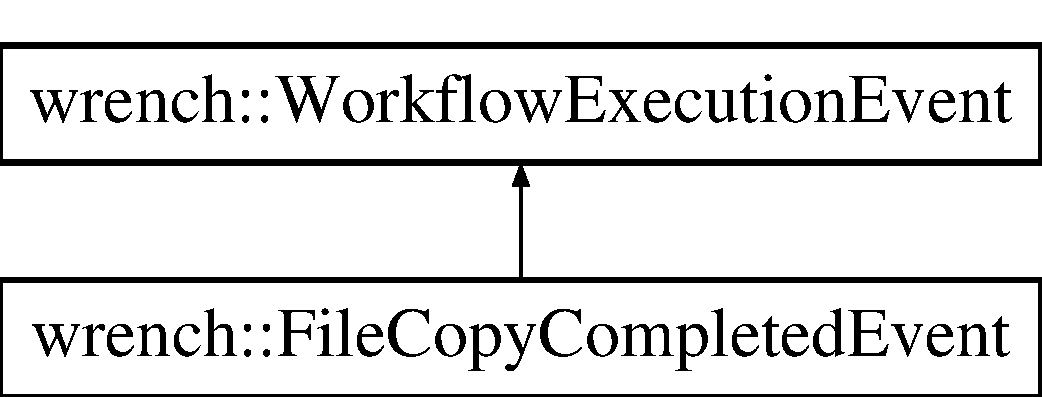
\includegraphics[height=2.000000cm]{classwrench_1_1_file_copy_completed_event}
\end{center}
\end{figure}
\subsection*{Public Attributes}
\begin{DoxyCompactItemize}
\item 
\mbox{\Hypertarget{classwrench_1_1_file_copy_completed_event_aed62752926d496a4335ec83dd5b8b028}\label{classwrench_1_1_file_copy_completed_event_aed62752926d496a4335ec83dd5b8b028}} 
\hyperlink{classwrench_1_1_workflow_file}{Workflow\+File} $\ast$ \hyperlink{classwrench_1_1_file_copy_completed_event_aed62752926d496a4335ec83dd5b8b028}{file}
\begin{DoxyCompactList}\small\item\em The workflow file that has successfully been copied. \end{DoxyCompactList}\item 
\mbox{\Hypertarget{classwrench_1_1_file_copy_completed_event_a5c2d148a0ed5b983d2107dd06e6beefe}\label{classwrench_1_1_file_copy_completed_event_a5c2d148a0ed5b983d2107dd06e6beefe}} 
\hyperlink{classwrench_1_1_file_registry_service}{File\+Registry\+Service} $\ast$ \hyperlink{classwrench_1_1_file_copy_completed_event_a5c2d148a0ed5b983d2107dd06e6beefe}{file\+\_\+registry\+\_\+service}
\begin{DoxyCompactList}\small\item\em The file registry service that was supposed to be updated (or nullptr if none) \end{DoxyCompactList}\item 
\mbox{\Hypertarget{classwrench_1_1_file_copy_completed_event_a6f72ffd664cfd233ae769b2985d85360}\label{classwrench_1_1_file_copy_completed_event_a6f72ffd664cfd233ae769b2985d85360}} 
bool \hyperlink{classwrench_1_1_file_copy_completed_event_a6f72ffd664cfd233ae769b2985d85360}{file\+\_\+registry\+\_\+service\+\_\+updated}
\begin{DoxyCompactList}\small\item\em Whether the file registry service (if any) has been successfully updated. \end{DoxyCompactList}\item 
\mbox{\Hypertarget{classwrench_1_1_file_copy_completed_event_a58c97ffa789f6422b1e1798f104e80bf}\label{classwrench_1_1_file_copy_completed_event_a58c97ffa789f6422b1e1798f104e80bf}} 
\hyperlink{classwrench_1_1_storage_service}{Storage\+Service} $\ast$ \hyperlink{classwrench_1_1_file_copy_completed_event_a58c97ffa789f6422b1e1798f104e80bf}{storage\+\_\+service}
\begin{DoxyCompactList}\small\item\em The storage service to which the file has been copied. \end{DoxyCompactList}\end{DoxyCompactItemize}
\subsection*{Additional Inherited Members}


\subsection{Detailed Description}
A \char`\"{}file copy has completed\char`\"{} \hyperlink{classwrench_1_1_workflow_execution_event}{Workflow\+Execution\+Event}. 

The documentation for this class was generated from the following file\+:\begin{DoxyCompactItemize}
\item 
/\+Users/rafsilva/\+Documents/isi/workspace/wrench/wrench/include/wrench/workflow/execution\+\_\+events/Workflow\+Execution\+Event.\+h\end{DoxyCompactItemize}

\hypertarget{classwrench_1_1_file_copy_failed_event}{}\section{wrench\+:\+:File\+Copy\+Failed\+Event Class Reference}
\label{classwrench_1_1_file_copy_failed_event}\index{wrench\+::\+File\+Copy\+Failed\+Event@{wrench\+::\+File\+Copy\+Failed\+Event}}


A \char`\"{}file copy has failed\char`\"{} \hyperlink{classwrench_1_1_workflow_execution_event}{Workflow\+Execution\+Event}.  




{\ttfamily \#include $<$Workflow\+Execution\+Event.\+h$>$}

Inheritance diagram for wrench\+:\+:File\+Copy\+Failed\+Event\+:\begin{figure}[H]
\begin{center}
\leavevmode
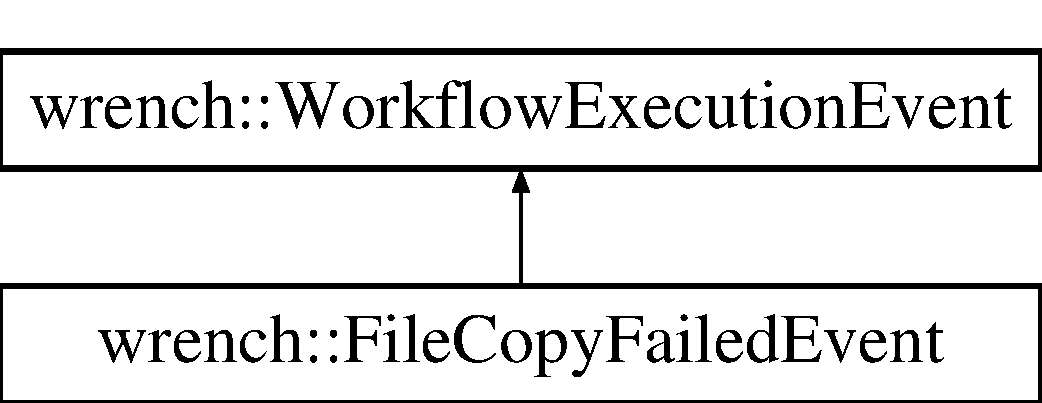
\includegraphics[height=2.000000cm]{classwrench_1_1_file_copy_failed_event}
\end{center}
\end{figure}
\subsection*{Public Attributes}
\begin{DoxyCompactItemize}
\item 
\mbox{\Hypertarget{classwrench_1_1_file_copy_failed_event_a8d3e5e8ce73f3ac145eb5046e0e79833}\label{classwrench_1_1_file_copy_failed_event_a8d3e5e8ce73f3ac145eb5046e0e79833}} 
std\+::shared\+\_\+ptr$<$ \hyperlink{classwrench_1_1_failure_cause}{Failure\+Cause} $>$ \hyperlink{classwrench_1_1_file_copy_failed_event_a8d3e5e8ce73f3ac145eb5046e0e79833}{failure\+\_\+cause}
\begin{DoxyCompactList}\small\item\em The cause of the failure. \end{DoxyCompactList}\item 
\mbox{\Hypertarget{classwrench_1_1_file_copy_failed_event_ab15883f629da5271f8cb3f0e2add0345}\label{classwrench_1_1_file_copy_failed_event_ab15883f629da5271f8cb3f0e2add0345}} 
\hyperlink{classwrench_1_1_workflow_file}{Workflow\+File} $\ast$ \hyperlink{classwrench_1_1_file_copy_failed_event_ab15883f629da5271f8cb3f0e2add0345}{file}
\begin{DoxyCompactList}\small\item\em The workflow file that has failed to be copied. \end{DoxyCompactList}\item 
\mbox{\Hypertarget{classwrench_1_1_file_copy_failed_event_ae24d988402fcdd2d3d114d2f1787096e}\label{classwrench_1_1_file_copy_failed_event_ae24d988402fcdd2d3d114d2f1787096e}} 
\hyperlink{classwrench_1_1_storage_service}{Storage\+Service} $\ast$ \hyperlink{classwrench_1_1_file_copy_failed_event_ae24d988402fcdd2d3d114d2f1787096e}{storage\+\_\+service}
\begin{DoxyCompactList}\small\item\em The storage service on which it was supposed to be copied. \end{DoxyCompactList}\end{DoxyCompactItemize}
\subsection*{Additional Inherited Members}


\subsection{Detailed Description}
A \char`\"{}file copy has failed\char`\"{} \hyperlink{classwrench_1_1_workflow_execution_event}{Workflow\+Execution\+Event}. 

The documentation for this class was generated from the following file\+:\begin{DoxyCompactItemize}
\item 
/\+Users/rafsilva/\+Documents/isi/workspace/wrench/wrench/include/wrench/workflow/execution\+\_\+events/Workflow\+Execution\+Event.\+h\end{DoxyCompactItemize}

\hypertarget{structwrench_1_1_simulation_timestamp_file_copy_1_1_file_location}{}\section{wrench\+:\+:Simulation\+Timestamp\+File\+Copy\+:\+:File\+Location Struct Reference}
\label{structwrench_1_1_simulation_timestamp_file_copy_1_1_file_location}\index{wrench\+::\+Simulation\+Timestamp\+File\+Copy\+::\+File\+Location@{wrench\+::\+Simulation\+Timestamp\+File\+Copy\+::\+File\+Location}}


A file location struct that contains the storage service and partition where a file is located.  




{\ttfamily \#include $<$Simulation\+Timestamp\+Types.\+h$>$}

\subsection*{Public Member Functions}
\begin{DoxyCompactItemize}
\item 
\mbox{\Hypertarget{structwrench_1_1_simulation_timestamp_file_copy_1_1_file_location_ae7c84b7e0d04c47b45b73a1c606388cf}\label{structwrench_1_1_simulation_timestamp_file_copy_1_1_file_location_ae7c84b7e0d04c47b45b73a1c606388cf}} 
{\bfseries File\+Location} (\hyperlink{classwrench_1_1_storage_service}{Storage\+Service} $\ast$storage\+\_\+service, std\+::string partition)
\item 
\mbox{\Hypertarget{structwrench_1_1_simulation_timestamp_file_copy_1_1_file_location_aeba929897e5efd58f2912f4ed41e19cd}\label{structwrench_1_1_simulation_timestamp_file_copy_1_1_file_location_aeba929897e5efd58f2912f4ed41e19cd}} 
bool {\bfseries operator!=} (const \hyperlink{structwrench_1_1_simulation_timestamp_file_copy_1_1_file_location}{File\+Location} \&rhs)
\item 
\mbox{\Hypertarget{structwrench_1_1_simulation_timestamp_file_copy_1_1_file_location_a3dff7db2ffe47741dfd8e5b3ea39c51d}\label{structwrench_1_1_simulation_timestamp_file_copy_1_1_file_location_a3dff7db2ffe47741dfd8e5b3ea39c51d}} 
bool {\bfseries operator==} (const \hyperlink{structwrench_1_1_simulation_timestamp_file_copy_1_1_file_location}{File\+Location} \&rhs)
\end{DoxyCompactItemize}
\subsection*{Public Attributes}
\begin{DoxyCompactItemize}
\item 
\mbox{\Hypertarget{structwrench_1_1_simulation_timestamp_file_copy_1_1_file_location_abbfd743a39bc124ef6dab2ca053a4989}\label{structwrench_1_1_simulation_timestamp_file_copy_1_1_file_location_abbfd743a39bc124ef6dab2ca053a4989}} 
std\+::string {\bfseries partition}
\item 
\mbox{\Hypertarget{structwrench_1_1_simulation_timestamp_file_copy_1_1_file_location_aee633ee71f58b8a4474ea9ad5db1e1fd}\label{structwrench_1_1_simulation_timestamp_file_copy_1_1_file_location_aee633ee71f58b8a4474ea9ad5db1e1fd}} 
\hyperlink{classwrench_1_1_storage_service}{Storage\+Service} $\ast$ {\bfseries storage\+\_\+service}
\end{DoxyCompactItemize}


\subsection{Detailed Description}
A file location struct that contains the storage service and partition where a file is located. 

The documentation for this struct was generated from the following file\+:\begin{DoxyCompactItemize}
\item 
/\+Users/rafsilva/\+Documents/isi/workspace/wrench/wrench/include/wrench/simulation/Simulation\+Timestamp\+Types.\+h\end{DoxyCompactItemize}

\hypertarget{classwrench_1_1_file_not_found}{}\section{wrench\+:\+:File\+Not\+Found Class Reference}
\label{classwrench_1_1_file_not_found}\index{wrench\+::\+File\+Not\+Found@{wrench\+::\+File\+Not\+Found}}


A \char`\"{}file was not found\char`\"{} failure cause.  




{\ttfamily \#include $<$Failure\+Cause.\+h$>$}

Inheritance diagram for wrench\+:\+:File\+Not\+Found\+:\begin{figure}[H]
\begin{center}
\leavevmode
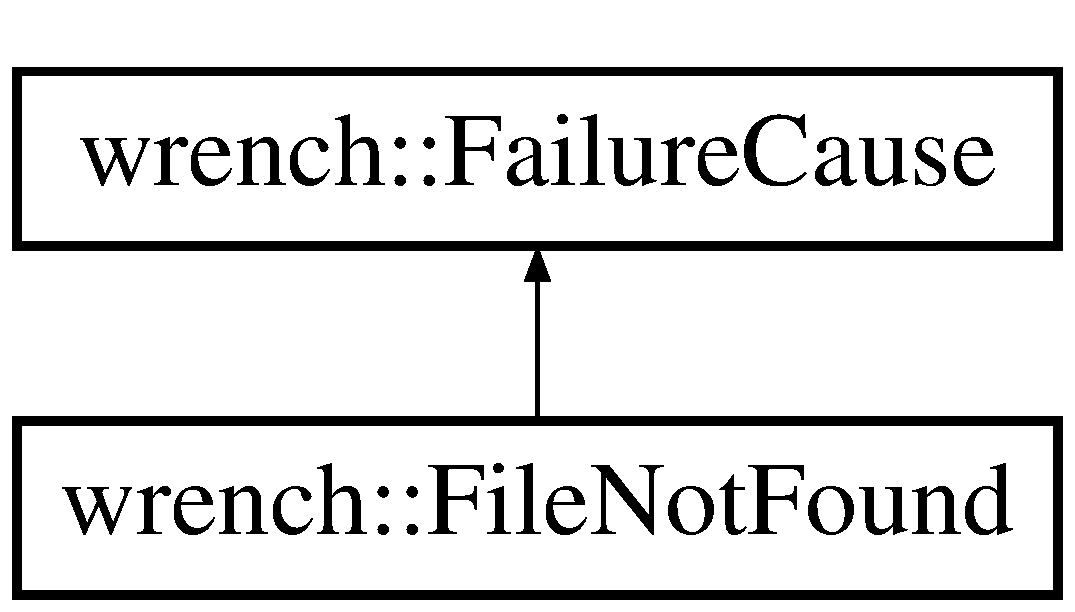
\includegraphics[height=2.000000cm]{classwrench_1_1_file_not_found}
\end{center}
\end{figure}
\subsection*{Public Member Functions}
\begin{DoxyCompactItemize}
\item 
\hyperlink{classwrench_1_1_workflow_file}{Workflow\+File} $\ast$ \hyperlink{classwrench_1_1_file_not_found_aa89df5eaeb42af70876ac6ce084de33d}{get\+File} ()
\begin{DoxyCompactList}\small\item\em Getter. \end{DoxyCompactList}\item 
\hyperlink{classwrench_1_1_storage_service}{Storage\+Service} $\ast$ \hyperlink{classwrench_1_1_file_not_found_ac831b3a371f81e56bfac869fd4113514}{get\+Storage\+Service} ()
\begin{DoxyCompactList}\small\item\em Getter. \end{DoxyCompactList}\item 
std\+::string \hyperlink{classwrench_1_1_file_not_found_ac9c3bdcc58b4626a0f3de0b4288bf4b4}{to\+String} ()
\begin{DoxyCompactList}\small\item\em Get the human-\/readable failure message. \end{DoxyCompactList}\end{DoxyCompactItemize}
\subsection*{Additional Inherited Members}


\subsection{Detailed Description}
A \char`\"{}file was not found\char`\"{} failure cause. 

\subsection{Member Function Documentation}
\mbox{\Hypertarget{classwrench_1_1_file_not_found_aa89df5eaeb42af70876ac6ce084de33d}\label{classwrench_1_1_file_not_found_aa89df5eaeb42af70876ac6ce084de33d}} 
\index{wrench\+::\+File\+Not\+Found@{wrench\+::\+File\+Not\+Found}!get\+File@{get\+File}}
\index{get\+File@{get\+File}!wrench\+::\+File\+Not\+Found@{wrench\+::\+File\+Not\+Found}}
\subsubsection{\texorpdfstring{get\+File()}{getFile()}}
{\footnotesize\ttfamily \hyperlink{classwrench_1_1_workflow_file}{Workflow\+File} $\ast$ wrench\+::\+File\+Not\+Found\+::get\+File (\begin{DoxyParamCaption}{ }\end{DoxyParamCaption})}



Getter. 

\begin{DoxyReturn}{Returns}
the file 
\end{DoxyReturn}
\mbox{\Hypertarget{classwrench_1_1_file_not_found_ac831b3a371f81e56bfac869fd4113514}\label{classwrench_1_1_file_not_found_ac831b3a371f81e56bfac869fd4113514}} 
\index{wrench\+::\+File\+Not\+Found@{wrench\+::\+File\+Not\+Found}!get\+Storage\+Service@{get\+Storage\+Service}}
\index{get\+Storage\+Service@{get\+Storage\+Service}!wrench\+::\+File\+Not\+Found@{wrench\+::\+File\+Not\+Found}}
\subsubsection{\texorpdfstring{get\+Storage\+Service()}{getStorageService()}}
{\footnotesize\ttfamily \hyperlink{classwrench_1_1_storage_service}{Storage\+Service} $\ast$ wrench\+::\+File\+Not\+Found\+::get\+Storage\+Service (\begin{DoxyParamCaption}{ }\end{DoxyParamCaption})}



Getter. 

\begin{DoxyReturn}{Returns}
the storage service 
\end{DoxyReturn}
\mbox{\Hypertarget{classwrench_1_1_file_not_found_ac9c3bdcc58b4626a0f3de0b4288bf4b4}\label{classwrench_1_1_file_not_found_ac9c3bdcc58b4626a0f3de0b4288bf4b4}} 
\index{wrench\+::\+File\+Not\+Found@{wrench\+::\+File\+Not\+Found}!to\+String@{to\+String}}
\index{to\+String@{to\+String}!wrench\+::\+File\+Not\+Found@{wrench\+::\+File\+Not\+Found}}
\subsubsection{\texorpdfstring{to\+String()}{toString()}}
{\footnotesize\ttfamily std\+::string wrench\+::\+File\+Not\+Found\+::to\+String (\begin{DoxyParamCaption}{ }\end{DoxyParamCaption})\hspace{0.3cm}{\ttfamily [virtual]}}



Get the human-\/readable failure message. 

\begin{DoxyReturn}{Returns}
the message 
\end{DoxyReturn}


Implements \hyperlink{classwrench_1_1_failure_cause_afbad248ebe902409f2cd4f1d6f2b867d}{wrench\+::\+Failure\+Cause}.



The documentation for this class was generated from the following files\+:\begin{DoxyCompactItemize}
\item 
/\+Users/rafsilva/\+Documents/isi/workspace/wrench/wrench/include/wrench/workflow/execution\+\_\+events/Failure\+Cause.\+h\item 
/\+Users/rafsilva/\+Documents/isi/workspace/wrench/wrench/src/wrench/workflow/execution\+\_\+events/Failure\+Cause.\+cpp\end{DoxyCompactItemize}

\hypertarget{classwrench_1_1_file_registry_service}{}\section{wrench\+:\+:File\+Registry\+Service Class Reference}
\label{classwrench_1_1_file_registry_service}\index{wrench\+::\+File\+Registry\+Service@{wrench\+::\+File\+Registry\+Service}}


A file registry service (a.\+k.\+a. replica catalog) that holds a database of which files are available at which storage services. More specifically, the database holds a set of $<$file, storage service$>$ entries. A \hyperlink{classwrench_1_1_w_m_s}{W\+MS} can add, lookup, and remove entries at will from this database.  




{\ttfamily \#include $<$File\+Registry\+Service.\+h$>$}

Inheritance diagram for wrench\+:\+:File\+Registry\+Service\+:\begin{figure}[H]
\begin{center}
\leavevmode
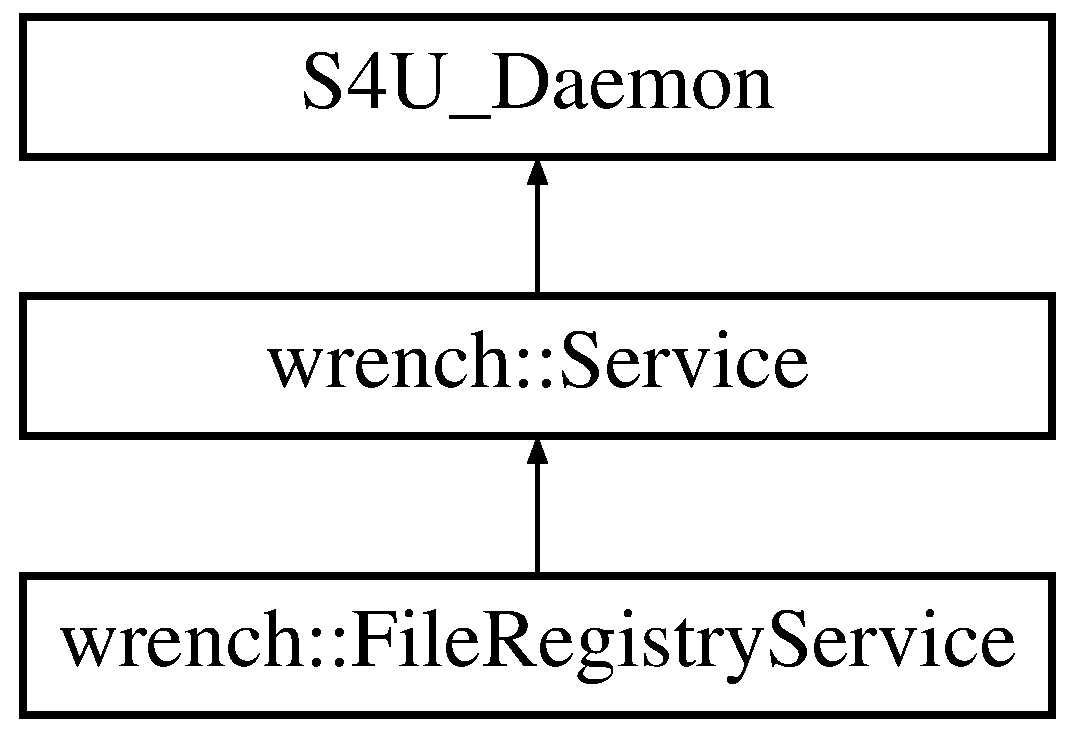
\includegraphics[height=3.000000cm]{classwrench_1_1_file_registry_service}
\end{center}
\end{figure}
\subsection*{Public Member Functions}
\begin{DoxyCompactItemize}
\item 
\hyperlink{classwrench_1_1_file_registry_service_ab5b1061fc26163f291e905c27bdbf114}{File\+Registry\+Service} (std\+::string \hyperlink{classwrench_1_1_s4_u___daemon_a52bc0b9a6cd248310749dac086819f00}{hostname}, std\+::map$<$ std\+::string, std\+::string $>$ \hyperlink{classwrench_1_1_service_a032143b1e2d7296dde9b4ca1e34845ce}{property\+\_\+list}=\{\}, std\+::map$<$ std\+::string, std\+::string $>$ \hyperlink{classwrench_1_1_service_a63865f20c92027ab626ab1347b0099d2}{messagepayload\+\_\+list}=\{\})
\begin{DoxyCompactList}\small\item\em Constructor. \end{DoxyCompactList}\item 
void \hyperlink{classwrench_1_1_file_registry_service_a6c630119b5168fa84ea923217ee02243}{add\+Entry} (\hyperlink{classwrench_1_1_workflow_file}{Workflow\+File} $\ast$file, \hyperlink{classwrench_1_1_storage_service}{Storage\+Service} $\ast$storage\+\_\+service)
\begin{DoxyCompactList}\small\item\em Add an entry. \end{DoxyCompactList}\item 
std\+::set$<$ \hyperlink{classwrench_1_1_storage_service}{Storage\+Service} $\ast$ $>$ \hyperlink{classwrench_1_1_file_registry_service_a380277028177601cd601c8d8603d47f6}{lookup\+Entry} (\hyperlink{classwrench_1_1_workflow_file}{Workflow\+File} $\ast$file)
\begin{DoxyCompactList}\small\item\em Lookup entries for a file. \end{DoxyCompactList}\item 
std\+::map$<$ double, \hyperlink{classwrench_1_1_storage_service}{Storage\+Service} $\ast$ $>$ \hyperlink{classwrench_1_1_file_registry_service_a729671ba5d3f3d0da7f3e15058515aa7}{lookup\+Entry} (\hyperlink{classwrench_1_1_workflow_file}{Workflow\+File} $\ast$file, std\+::string reference\+\_\+host, \hyperlink{classwrench_1_1_network_proximity_service}{Network\+Proximity\+Service} $\ast$)
\begin{DoxyCompactList}\small\item\em Lookup entries for a file, including for each entry a network distance from a reference host (as determined by a network proximity service) \end{DoxyCompactList}\item 
void \hyperlink{classwrench_1_1_file_registry_service_a3e5d8d7503c2d3ad422b35c598647d82}{remove\+Entry} (\hyperlink{classwrench_1_1_workflow_file}{Workflow\+File} $\ast$file, \hyperlink{classwrench_1_1_storage_service}{Storage\+Service} $\ast$storage\+\_\+service)
\begin{DoxyCompactList}\small\item\em Remove an entry. \end{DoxyCompactList}\end{DoxyCompactItemize}
\subsection*{Additional Inherited Members}


\subsection{Detailed Description}
A file registry service (a.\+k.\+a. replica catalog) that holds a database of which files are available at which storage services. More specifically, the database holds a set of $<$file, storage service$>$ entries. A \hyperlink{classwrench_1_1_w_m_s}{W\+MS} can add, lookup, and remove entries at will from this database. 

\subsection{Constructor \& Destructor Documentation}
\mbox{\Hypertarget{classwrench_1_1_file_registry_service_ab5b1061fc26163f291e905c27bdbf114}\label{classwrench_1_1_file_registry_service_ab5b1061fc26163f291e905c27bdbf114}} 
\index{wrench\+::\+File\+Registry\+Service@{wrench\+::\+File\+Registry\+Service}!File\+Registry\+Service@{File\+Registry\+Service}}
\index{File\+Registry\+Service@{File\+Registry\+Service}!wrench\+::\+File\+Registry\+Service@{wrench\+::\+File\+Registry\+Service}}
\subsubsection{\texorpdfstring{File\+Registry\+Service()}{FileRegistryService()}}
{\footnotesize\ttfamily wrench\+::\+File\+Registry\+Service\+::\+File\+Registry\+Service (\begin{DoxyParamCaption}\item[{std\+::string}]{hostname,  }\item[{std\+::map$<$ std\+::string, std\+::string $>$}]{property\+\_\+list = {\ttfamily \{\}},  }\item[{std\+::map$<$ std\+::string, std\+::string $>$}]{messagepayload\+\_\+list = {\ttfamily \{\}} }\end{DoxyParamCaption})}



Constructor. 


\begin{DoxyParams}{Parameters}
{\em hostname} & the hostname on which to start the service \\
\hline
{\em property\+\_\+list} & a property list (\{\} means \char`\"{}use all defaults\char`\"{}) \\
\hline
{\em messagepayload\+\_\+list} & a message payload list (\{\} means \char`\"{}use all defaults\char`\"{}) \\
\hline
\end{DoxyParams}


\subsection{Member Function Documentation}
\mbox{\Hypertarget{classwrench_1_1_file_registry_service_a6c630119b5168fa84ea923217ee02243}\label{classwrench_1_1_file_registry_service_a6c630119b5168fa84ea923217ee02243}} 
\index{wrench\+::\+File\+Registry\+Service@{wrench\+::\+File\+Registry\+Service}!add\+Entry@{add\+Entry}}
\index{add\+Entry@{add\+Entry}!wrench\+::\+File\+Registry\+Service@{wrench\+::\+File\+Registry\+Service}}
\subsubsection{\texorpdfstring{add\+Entry()}{addEntry()}}
{\footnotesize\ttfamily void wrench\+::\+File\+Registry\+Service\+::add\+Entry (\begin{DoxyParamCaption}\item[{\hyperlink{classwrench_1_1_workflow_file}{Workflow\+File} $\ast$}]{file,  }\item[{\hyperlink{classwrench_1_1_storage_service}{Storage\+Service} $\ast$}]{storage\+\_\+service }\end{DoxyParamCaption})}



Add an entry. 


\begin{DoxyParams}{Parameters}
{\em file} & a file \\
\hline
{\em storage\+\_\+service} & a storage\+\_\+service\\
\hline
\end{DoxyParams}

\begin{DoxyExceptions}{Exceptions}
{\em \hyperlink{classwrench_1_1_workflow_execution_exception}{Workflow\+Execution\+Exception}} & \\
\hline
{\em std\+::invalid\+\_\+argument} & \\
\hline
{\em std\+::runtime\+\_\+error} & \\
\hline
\end{DoxyExceptions}
\mbox{\Hypertarget{classwrench_1_1_file_registry_service_a380277028177601cd601c8d8603d47f6}\label{classwrench_1_1_file_registry_service_a380277028177601cd601c8d8603d47f6}} 
\index{wrench\+::\+File\+Registry\+Service@{wrench\+::\+File\+Registry\+Service}!lookup\+Entry@{lookup\+Entry}}
\index{lookup\+Entry@{lookup\+Entry}!wrench\+::\+File\+Registry\+Service@{wrench\+::\+File\+Registry\+Service}}
\subsubsection{\texorpdfstring{lookup\+Entry()}{lookupEntry()}\hspace{0.1cm}{\footnotesize\ttfamily [1/2]}}
{\footnotesize\ttfamily std\+::set$<$ \hyperlink{classwrench_1_1_storage_service}{Storage\+Service} $\ast$ $>$ wrench\+::\+File\+Registry\+Service\+::lookup\+Entry (\begin{DoxyParamCaption}\item[{\hyperlink{classwrench_1_1_workflow_file}{Workflow\+File} $\ast$}]{file }\end{DoxyParamCaption})}



Lookup entries for a file. 


\begin{DoxyParams}{Parameters}
{\em file} & the file to lookup \\
\hline
\end{DoxyParams}
\begin{DoxyReturn}{Returns}
The list of storage services that hold a copy of the file
\end{DoxyReturn}

\begin{DoxyExceptions}{Exceptions}
{\em \hyperlink{classwrench_1_1_workflow_execution_exception}{Workflow\+Execution\+Exception}} & \\
\hline
{\em std\+::invalid\+\_\+argument} & \\
\hline
{\em std\+::runtime\+\_\+error} & \\
\hline
\end{DoxyExceptions}
\mbox{\Hypertarget{classwrench_1_1_file_registry_service_a729671ba5d3f3d0da7f3e15058515aa7}\label{classwrench_1_1_file_registry_service_a729671ba5d3f3d0da7f3e15058515aa7}} 
\index{wrench\+::\+File\+Registry\+Service@{wrench\+::\+File\+Registry\+Service}!lookup\+Entry@{lookup\+Entry}}
\index{lookup\+Entry@{lookup\+Entry}!wrench\+::\+File\+Registry\+Service@{wrench\+::\+File\+Registry\+Service}}
\subsubsection{\texorpdfstring{lookup\+Entry()}{lookupEntry()}\hspace{0.1cm}{\footnotesize\ttfamily [2/2]}}
{\footnotesize\ttfamily std\+::map$<$ double, \hyperlink{classwrench_1_1_storage_service}{Storage\+Service} $\ast$ $>$ wrench\+::\+File\+Registry\+Service\+::lookup\+Entry (\begin{DoxyParamCaption}\item[{\hyperlink{classwrench_1_1_workflow_file}{Workflow\+File} $\ast$}]{file,  }\item[{std\+::string}]{reference\+\_\+host,  }\item[{\hyperlink{classwrench_1_1_network_proximity_service}{Network\+Proximity\+Service} $\ast$}]{network\+\_\+proximity\+\_\+service }\end{DoxyParamCaption})}



Lookup entries for a file, including for each entry a network distance from a reference host (as determined by a network proximity service) 


\begin{DoxyParams}{Parameters}
{\em file} & the file to lookup \\
\hline
{\em reference\+\_\+host} & reference host from which network proximity values are to be measured \\
\hline
{\em network\+\_\+proximity\+\_\+service} & the network proximity service to use\\
\hline
\end{DoxyParams}
\begin{DoxyReturn}{Returns}
a map of $<$distance , storage service$>$ pairs 
\end{DoxyReturn}
\mbox{\Hypertarget{classwrench_1_1_file_registry_service_a3e5d8d7503c2d3ad422b35c598647d82}\label{classwrench_1_1_file_registry_service_a3e5d8d7503c2d3ad422b35c598647d82}} 
\index{wrench\+::\+File\+Registry\+Service@{wrench\+::\+File\+Registry\+Service}!remove\+Entry@{remove\+Entry}}
\index{remove\+Entry@{remove\+Entry}!wrench\+::\+File\+Registry\+Service@{wrench\+::\+File\+Registry\+Service}}
\subsubsection{\texorpdfstring{remove\+Entry()}{removeEntry()}}
{\footnotesize\ttfamily void wrench\+::\+File\+Registry\+Service\+::remove\+Entry (\begin{DoxyParamCaption}\item[{\hyperlink{classwrench_1_1_workflow_file}{Workflow\+File} $\ast$}]{file,  }\item[{\hyperlink{classwrench_1_1_storage_service}{Storage\+Service} $\ast$}]{storage\+\_\+service }\end{DoxyParamCaption})}



Remove an entry. 


\begin{DoxyParams}{Parameters}
{\em file} & a file \\
\hline
{\em storage\+\_\+service} & a storage service\\
\hline
\end{DoxyParams}

\begin{DoxyExceptions}{Exceptions}
{\em \hyperlink{classwrench_1_1_workflow_execution_exception}{Workflow\+Execution\+Exception}} & \\
\hline
{\em std\+::invalid\+\_\+argument} & \\
\hline
{\em std\+::runtime\+\_\+error} & \\
\hline
\end{DoxyExceptions}


The documentation for this class was generated from the following files\+:\begin{DoxyCompactItemize}
\item 
/\+Users/rafsilva/\+Documents/isi/workspace/wrench/wrench/include/wrench/services/file\+\_\+registry/File\+Registry\+Service.\+h\item 
/\+Users/rafsilva/\+Documents/isi/workspace/wrench/wrench/src/wrench/services/file\+\_\+registry/File\+Registry\+Service.\+cpp\end{DoxyCompactItemize}

\hypertarget{classwrench_1_1_file_registry_service_message_payload}{}\section{wrench\+:\+:File\+Registry\+Service\+Message\+Payload Class Reference}
\label{classwrench_1_1_file_registry_service_message_payload}\index{wrench\+::\+File\+Registry\+Service\+Message\+Payload@{wrench\+::\+File\+Registry\+Service\+Message\+Payload}}


Configurable message payload for a \hyperlink{classwrench_1_1_file_registry_service}{File\+Registry\+Service}.  




{\ttfamily \#include $<$File\+Registry\+Service\+Message\+Payload.\+h$>$}

Inheritance diagram for wrench\+:\+:File\+Registry\+Service\+Message\+Payload\+:\begin{figure}[H]
\begin{center}
\leavevmode
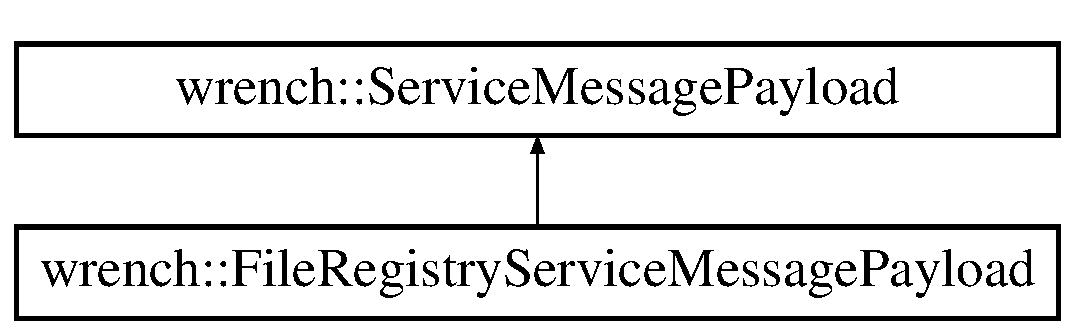
\includegraphics[height=2.000000cm]{classwrench_1_1_file_registry_service_message_payload}
\end{center}
\end{figure}
\subsection*{Static Public Attributes}
\begin{DoxyCompactItemize}
\item 
\mbox{\Hypertarget{classwrench_1_1_file_registry_service_message_payload_a4db8dcf568d85fafc162d0d192658e50}\label{classwrench_1_1_file_registry_service_message_payload_a4db8dcf568d85fafc162d0d192658e50}} 
static const std\+::string \hyperlink{classwrench_1_1_file_registry_service_message_payload_a4db8dcf568d85fafc162d0d192658e50}{A\+D\+D\+\_\+\+E\+N\+T\+R\+Y\+\_\+\+A\+N\+S\+W\+E\+R\+\_\+\+M\+E\+S\+S\+A\+G\+E\+\_\+\+P\+A\+Y\+L\+O\+AD}
\begin{DoxyCompactList}\small\item\em The number of bytes in the control message sent by the daemon to answer an entry addition request. \end{DoxyCompactList}\item 
\mbox{\Hypertarget{classwrench_1_1_file_registry_service_message_payload_ab2f9e325d2f97dc073f13ce34091cae8}\label{classwrench_1_1_file_registry_service_message_payload_ab2f9e325d2f97dc073f13ce34091cae8}} 
static const std\+::string \hyperlink{classwrench_1_1_file_registry_service_message_payload_ab2f9e325d2f97dc073f13ce34091cae8}{A\+D\+D\+\_\+\+E\+N\+T\+R\+Y\+\_\+\+R\+E\+Q\+U\+E\+S\+T\+\_\+\+M\+E\+S\+S\+A\+G\+E\+\_\+\+P\+A\+Y\+L\+O\+AD}
\begin{DoxyCompactList}\small\item\em The number of bytes in the control message sent to the daemon to cause it to add an entry. \end{DoxyCompactList}\item 
\mbox{\Hypertarget{classwrench_1_1_file_registry_service_message_payload_a17ec53dbb0ffdbc1245deac83817ba98}\label{classwrench_1_1_file_registry_service_message_payload_a17ec53dbb0ffdbc1245deac83817ba98}} 
static const std\+::string \hyperlink{classwrench_1_1_file_registry_service_message_payload_a17ec53dbb0ffdbc1245deac83817ba98}{F\+I\+L\+E\+\_\+\+L\+O\+O\+K\+U\+P\+\_\+\+A\+N\+S\+W\+E\+R\+\_\+\+M\+E\+S\+S\+A\+G\+E\+\_\+\+P\+A\+Y\+L\+O\+AD}
\begin{DoxyCompactList}\small\item\em The number of bytes per file location returned in an answer sent by the daemon to answer a file location request. \end{DoxyCompactList}\item 
\mbox{\Hypertarget{classwrench_1_1_file_registry_service_message_payload_a5f343d2e49893ac12df7f7112ce0fc2e}\label{classwrench_1_1_file_registry_service_message_payload_a5f343d2e49893ac12df7f7112ce0fc2e}} 
static const std\+::string \hyperlink{classwrench_1_1_file_registry_service_message_payload_a5f343d2e49893ac12df7f7112ce0fc2e}{F\+I\+L\+E\+\_\+\+L\+O\+O\+K\+U\+P\+\_\+\+R\+E\+Q\+U\+E\+S\+T\+\_\+\+M\+E\+S\+S\+A\+G\+E\+\_\+\+P\+A\+Y\+L\+O\+AD}
\begin{DoxyCompactList}\small\item\em The number of bytes in a request control message sent to the daemon to request a list of file locations. \end{DoxyCompactList}\item 
\mbox{\Hypertarget{classwrench_1_1_file_registry_service_message_payload_a143ee2e1ad8b0861b040fa67efb17db8}\label{classwrench_1_1_file_registry_service_message_payload_a143ee2e1ad8b0861b040fa67efb17db8}} 
static const std\+::string \hyperlink{classwrench_1_1_file_registry_service_message_payload_a143ee2e1ad8b0861b040fa67efb17db8}{R\+E\+M\+O\+V\+E\+\_\+\+E\+N\+T\+R\+Y\+\_\+\+A\+N\+S\+W\+E\+R\+\_\+\+M\+E\+S\+S\+A\+G\+E\+\_\+\+P\+A\+Y\+L\+O\+AD}
\begin{DoxyCompactList}\small\item\em The number of bytes in the control message sent by the daemon to answer an entry removal request. \end{DoxyCompactList}\item 
\mbox{\Hypertarget{classwrench_1_1_file_registry_service_message_payload_a1c16af0799b8ba26a3863ca0d253fbf1}\label{classwrench_1_1_file_registry_service_message_payload_a1c16af0799b8ba26a3863ca0d253fbf1}} 
static const std\+::string \hyperlink{classwrench_1_1_file_registry_service_message_payload_a1c16af0799b8ba26a3863ca0d253fbf1}{R\+E\+M\+O\+V\+E\+\_\+\+E\+N\+T\+R\+Y\+\_\+\+R\+E\+Q\+U\+E\+S\+T\+\_\+\+M\+E\+S\+S\+A\+G\+E\+\_\+\+P\+A\+Y\+L\+O\+AD}
\begin{DoxyCompactList}\small\item\em The number of bytes in the control message sent to the daemon to cause it to remove an entry. \end{DoxyCompactList}\end{DoxyCompactItemize}


\subsection{Detailed Description}
Configurable message payload for a \hyperlink{classwrench_1_1_file_registry_service}{File\+Registry\+Service}. 

The documentation for this class was generated from the following file\+:\begin{DoxyCompactItemize}
\item 
/\+Users/rafsilva/\+Documents/isi/workspace/wrench/wrench/include/wrench/services/file\+\_\+registry/File\+Registry\+Service\+Message\+Payload.\+h\end{DoxyCompactItemize}

\hypertarget{classwrench_1_1_file_registry_service_property}{}\section{wrench\+:\+:File\+Registry\+Service\+Property Class Reference}
\label{classwrench_1_1_file_registry_service_property}\index{wrench\+::\+File\+Registry\+Service\+Property@{wrench\+::\+File\+Registry\+Service\+Property}}


Configurable properties for a \hyperlink{classwrench_1_1_file_registry_service}{File\+Registry\+Service}.  




{\ttfamily \#include $<$File\+Registry\+Service\+Property.\+h$>$}

Inheritance diagram for wrench\+:\+:File\+Registry\+Service\+Property\+:\begin{figure}[H]
\begin{center}
\leavevmode
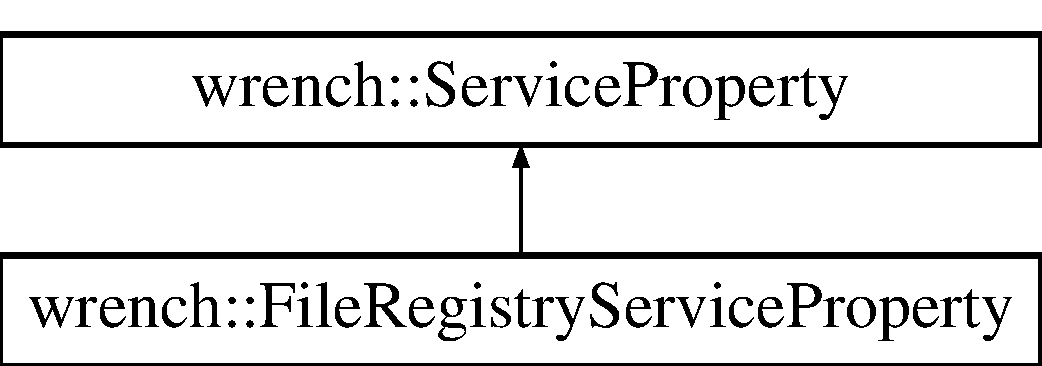
\includegraphics[height=2.000000cm]{classwrench_1_1_file_registry_service_property}
\end{center}
\end{figure}
\subsection*{Static Public Attributes}
\begin{DoxyCompactItemize}
\item 
\mbox{\Hypertarget{classwrench_1_1_file_registry_service_property_abd5bce0e04fa204f45aaaec00438eae7}\label{classwrench_1_1_file_registry_service_property_abd5bce0e04fa204f45aaaec00438eae7}} 
static const std\+::string \hyperlink{classwrench_1_1_file_registry_service_property_abd5bce0e04fa204f45aaaec00438eae7}{L\+O\+O\+K\+U\+P\+\_\+\+C\+O\+M\+P\+U\+T\+E\+\_\+\+C\+O\+ST}
\begin{DoxyCompactList}\small\item\em The computational cost, in flops, of looking up entries for a file. \end{DoxyCompactList}\end{DoxyCompactItemize}


\subsection{Detailed Description}
Configurable properties for a \hyperlink{classwrench_1_1_file_registry_service}{File\+Registry\+Service}. 

The documentation for this class was generated from the following file\+:\begin{DoxyCompactItemize}
\item 
/\+Users/rafsilva/\+Documents/isi/workspace/wrench/wrench/include/wrench/services/file\+\_\+registry/File\+Registry\+Service\+Property.\+h\end{DoxyCompactItemize}

\hypertarget{classwrench_1_1_functionality_not_available}{}\section{wrench\+:\+:Functionality\+Not\+Available Class Reference}
\label{classwrench_1_1_functionality_not_available}\index{wrench\+::\+Functionality\+Not\+Available@{wrench\+::\+Functionality\+Not\+Available}}


A \char`\"{}requested functionality is not available on that service\char`\"{} failure cause.  




{\ttfamily \#include $<$Failure\+Cause.\+h$>$}

Inheritance diagram for wrench\+:\+:Functionality\+Not\+Available\+:\begin{figure}[H]
\begin{center}
\leavevmode
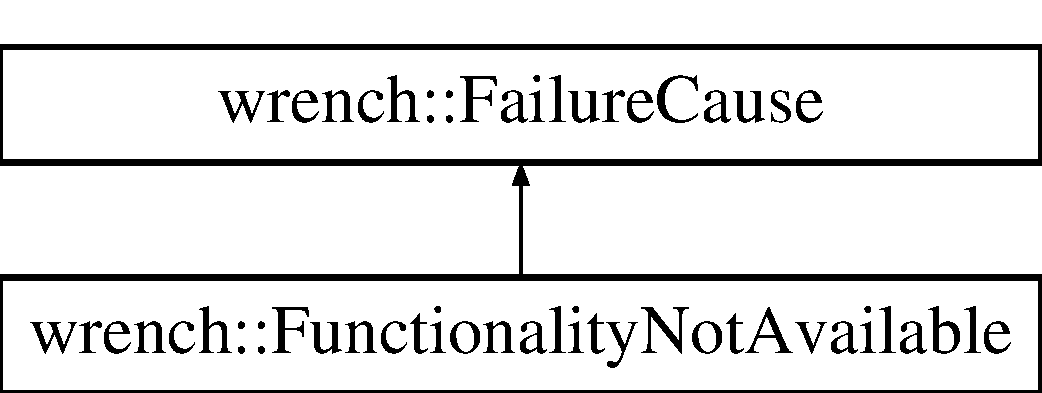
\includegraphics[height=2.000000cm]{classwrench_1_1_functionality_not_available}
\end{center}
\end{figure}
\subsection*{Public Member Functions}
\begin{DoxyCompactItemize}
\item 
\hyperlink{classwrench_1_1_functionality_not_available_a671895dd6d4ceef68e0311b47935b849}{Functionality\+Not\+Available} (\hyperlink{classwrench_1_1_service}{Service} $\ast$service, std\+::string functionality\+\_\+name)
\begin{DoxyCompactList}\small\item\em Constructor. \end{DoxyCompactList}\item 
std\+::string \hyperlink{classwrench_1_1_functionality_not_available_ab08a243a126daa6dfc538a7429f656b0}{get\+Functionality\+Name} ()
\begin{DoxyCompactList}\small\item\em Getter. \end{DoxyCompactList}\item 
\hyperlink{classwrench_1_1_service}{Service} $\ast$ \hyperlink{classwrench_1_1_functionality_not_available_a0c29976839df8de89c833e135f754bbb}{get\+Service} ()
\begin{DoxyCompactList}\small\item\em Getter. \end{DoxyCompactList}\item 
std\+::string \hyperlink{classwrench_1_1_functionality_not_available_af19ea11f7e3d50d0bea7c8a66b7b1221}{to\+String} ()
\begin{DoxyCompactList}\small\item\em Get the human-\/readable failure message. \end{DoxyCompactList}\end{DoxyCompactItemize}
\subsection*{Additional Inherited Members}


\subsection{Detailed Description}
A \char`\"{}requested functionality is not available on that service\char`\"{} failure cause. 

\subsection{Constructor \& Destructor Documentation}
\mbox{\Hypertarget{classwrench_1_1_functionality_not_available_a671895dd6d4ceef68e0311b47935b849}\label{classwrench_1_1_functionality_not_available_a671895dd6d4ceef68e0311b47935b849}} 
\index{wrench\+::\+Functionality\+Not\+Available@{wrench\+::\+Functionality\+Not\+Available}!Functionality\+Not\+Available@{Functionality\+Not\+Available}}
\index{Functionality\+Not\+Available@{Functionality\+Not\+Available}!wrench\+::\+Functionality\+Not\+Available@{wrench\+::\+Functionality\+Not\+Available}}
\subsubsection{\texorpdfstring{Functionality\+Not\+Available()}{FunctionalityNotAvailable()}}
{\footnotesize\ttfamily wrench\+::\+Functionality\+Not\+Available\+::\+Functionality\+Not\+Available (\begin{DoxyParamCaption}\item[{\hyperlink{classwrench_1_1_service}{Service} $\ast$}]{service,  }\item[{std\+::string}]{functionality\+\_\+name }\end{DoxyParamCaption})}



Constructor. 


\begin{DoxyParams}{Parameters}
{\em service} & the service \\
\hline
{\em functionality\+\_\+name} & a description of the functionality that\textquotesingle{}s not available \\
\hline
\end{DoxyParams}


\subsection{Member Function Documentation}
\mbox{\Hypertarget{classwrench_1_1_functionality_not_available_ab08a243a126daa6dfc538a7429f656b0}\label{classwrench_1_1_functionality_not_available_ab08a243a126daa6dfc538a7429f656b0}} 
\index{wrench\+::\+Functionality\+Not\+Available@{wrench\+::\+Functionality\+Not\+Available}!get\+Functionality\+Name@{get\+Functionality\+Name}}
\index{get\+Functionality\+Name@{get\+Functionality\+Name}!wrench\+::\+Functionality\+Not\+Available@{wrench\+::\+Functionality\+Not\+Available}}
\subsubsection{\texorpdfstring{get\+Functionality\+Name()}{getFunctionalityName()}}
{\footnotesize\ttfamily std\+::string wrench\+::\+Functionality\+Not\+Available\+::get\+Functionality\+Name (\begin{DoxyParamCaption}{ }\end{DoxyParamCaption})}



Getter. 

\begin{DoxyReturn}{Returns}
the functionality name 
\end{DoxyReturn}
\mbox{\Hypertarget{classwrench_1_1_functionality_not_available_a0c29976839df8de89c833e135f754bbb}\label{classwrench_1_1_functionality_not_available_a0c29976839df8de89c833e135f754bbb}} 
\index{wrench\+::\+Functionality\+Not\+Available@{wrench\+::\+Functionality\+Not\+Available}!get\+Service@{get\+Service}}
\index{get\+Service@{get\+Service}!wrench\+::\+Functionality\+Not\+Available@{wrench\+::\+Functionality\+Not\+Available}}
\subsubsection{\texorpdfstring{get\+Service()}{getService()}}
{\footnotesize\ttfamily \hyperlink{classwrench_1_1_service}{Service} $\ast$ wrench\+::\+Functionality\+Not\+Available\+::get\+Service (\begin{DoxyParamCaption}{ }\end{DoxyParamCaption})}



Getter. 

\begin{DoxyReturn}{Returns}
the service 
\end{DoxyReturn}
\mbox{\Hypertarget{classwrench_1_1_functionality_not_available_af19ea11f7e3d50d0bea7c8a66b7b1221}\label{classwrench_1_1_functionality_not_available_af19ea11f7e3d50d0bea7c8a66b7b1221}} 
\index{wrench\+::\+Functionality\+Not\+Available@{wrench\+::\+Functionality\+Not\+Available}!to\+String@{to\+String}}
\index{to\+String@{to\+String}!wrench\+::\+Functionality\+Not\+Available@{wrench\+::\+Functionality\+Not\+Available}}
\subsubsection{\texorpdfstring{to\+String()}{toString()}}
{\footnotesize\ttfamily std\+::string wrench\+::\+Functionality\+Not\+Available\+::to\+String (\begin{DoxyParamCaption}{ }\end{DoxyParamCaption})\hspace{0.3cm}{\ttfamily [virtual]}}



Get the human-\/readable failure message. 

\begin{DoxyReturn}{Returns}
the message 
\end{DoxyReturn}


Implements \hyperlink{classwrench_1_1_failure_cause_afbad248ebe902409f2cd4f1d6f2b867d}{wrench\+::\+Failure\+Cause}.



The documentation for this class was generated from the following files\+:\begin{DoxyCompactItemize}
\item 
/\+Users/rafsilva/\+Documents/isi/workspace/wrench/wrench/include/wrench/workflow/execution\+\_\+events/Failure\+Cause.\+h\item 
/\+Users/rafsilva/\+Documents/isi/workspace/wrench/wrench/src/wrench/workflow/execution\+\_\+events/Failure\+Cause.\+cpp\end{DoxyCompactItemize}

\hypertarget{classwrench_1_1_host_error}{}\section{wrench\+:\+:Host\+Error Class Reference}
\label{classwrench_1_1_host_error}\index{wrench\+::\+Host\+Error@{wrench\+::\+Host\+Error}}


A \char`\"{}host error\char`\"{} failure cause.  




{\ttfamily \#include $<$Failure\+Cause.\+h$>$}

Inheritance diagram for wrench\+:\+:Host\+Error\+:\begin{figure}[H]
\begin{center}
\leavevmode
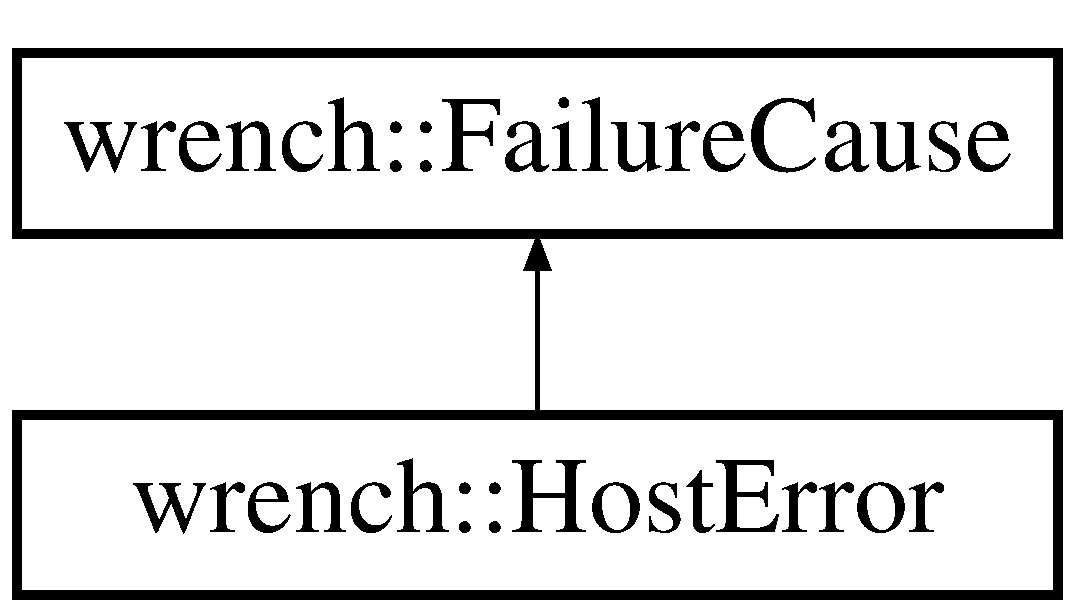
\includegraphics[height=2.000000cm]{classwrench_1_1_host_error}
\end{center}
\end{figure}
\subsection*{Public Member Functions}
\begin{DoxyCompactItemize}
\item 
std\+::string \hyperlink{classwrench_1_1_host_error_adacb96198ee8477b67fcac9ff8638266}{to\+String} ()
\begin{DoxyCompactList}\small\item\em Get the human-\/readable failure message. \end{DoxyCompactList}\end{DoxyCompactItemize}
\subsection*{Additional Inherited Members}


\subsection{Detailed Description}
A \char`\"{}host error\char`\"{} failure cause. 

\subsection{Member Function Documentation}
\mbox{\Hypertarget{classwrench_1_1_host_error_adacb96198ee8477b67fcac9ff8638266}\label{classwrench_1_1_host_error_adacb96198ee8477b67fcac9ff8638266}} 
\index{wrench\+::\+Host\+Error@{wrench\+::\+Host\+Error}!to\+String@{to\+String}}
\index{to\+String@{to\+String}!wrench\+::\+Host\+Error@{wrench\+::\+Host\+Error}}
\subsubsection{\texorpdfstring{to\+String()}{toString()}}
{\footnotesize\ttfamily std\+::string wrench\+::\+Host\+Error\+::to\+String (\begin{DoxyParamCaption}{ }\end{DoxyParamCaption})\hspace{0.3cm}{\ttfamily [virtual]}}



Get the human-\/readable failure message. 

\begin{DoxyReturn}{Returns}
the message 
\end{DoxyReturn}


Implements \hyperlink{classwrench_1_1_failure_cause_afbad248ebe902409f2cd4f1d6f2b867d}{wrench\+::\+Failure\+Cause}.



The documentation for this class was generated from the following files\+:\begin{DoxyCompactItemize}
\item 
/\+Users/rafsilva/\+Documents/isi/workspace/wrench/wrench/include/wrench/workflow/execution\+\_\+events/Failure\+Cause.\+h\item 
/\+Users/rafsilva/\+Documents/isi/workspace/wrench/wrench/src/wrench/workflow/execution\+\_\+events/Failure\+Cause.\+cpp\end{DoxyCompactItemize}

\hypertarget{classwrench_1_1_h_t_condor_central_manager_service}{}\section{wrench\+:\+:H\+T\+Condor\+Central\+Manager\+Service Class Reference}
\label{classwrench_1_1_h_t_condor_central_manager_service}\index{wrench\+::\+H\+T\+Condor\+Central\+Manager\+Service@{wrench\+::\+H\+T\+Condor\+Central\+Manager\+Service}}
Inheritance diagram for wrench\+:\+:H\+T\+Condor\+Central\+Manager\+Service\+:\begin{figure}[H]
\begin{center}
\leavevmode
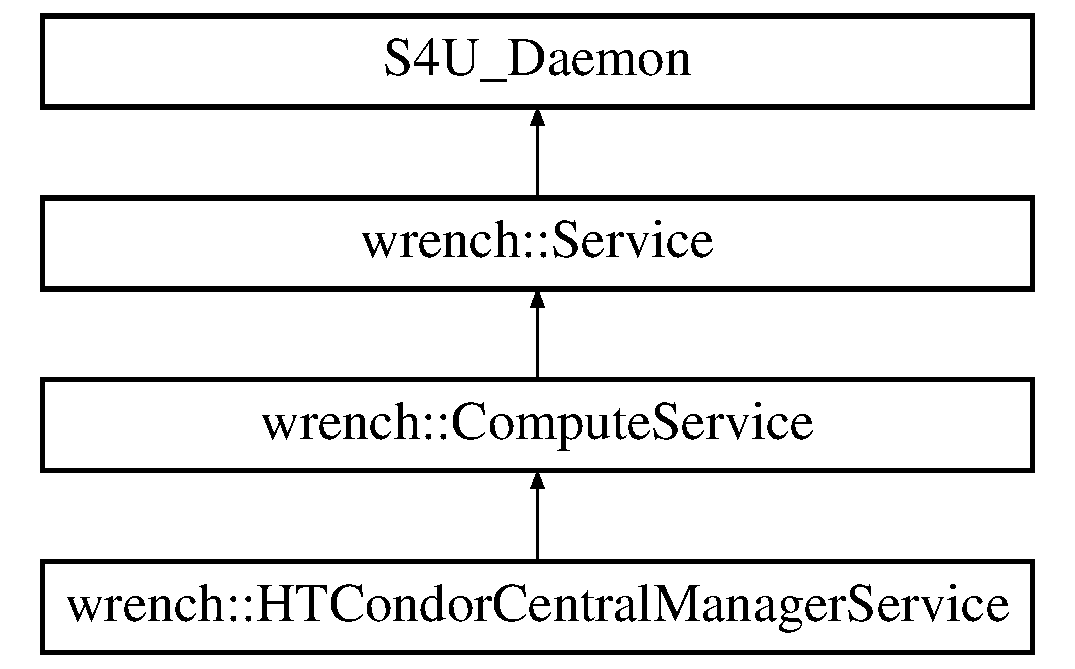
\includegraphics[height=4.000000cm]{classwrench_1_1_h_t_condor_central_manager_service}
\end{center}
\end{figure}
\subsection*{Public Member Functions}
\begin{DoxyCompactItemize}
\item 
\hyperlink{classwrench_1_1_h_t_condor_central_manager_service_acc295c6ed3ed9d036d72a41150f4a05a}{H\+T\+Condor\+Central\+Manager\+Service} (const std\+::string \&\hyperlink{classwrench_1_1_s4_u___daemon_a52bc0b9a6cd248310749dac086819f00}{hostname}, std\+::set$<$ \hyperlink{classwrench_1_1_compute_service}{Compute\+Service} $\ast$$>$ compute\+\_\+resources, std\+::map$<$ std\+::string, std\+::string $>$ \hyperlink{classwrench_1_1_service_a032143b1e2d7296dde9b4ca1e34845ce}{property\+\_\+list}=\{\}, std\+::map$<$ std\+::string, std\+::string $>$ \hyperlink{classwrench_1_1_service_a63865f20c92027ab626ab1347b0099d2}{messagepayload\+\_\+list}=\{\})
\begin{DoxyCompactList}\small\item\em Constructor. \end{DoxyCompactList}\item 
\mbox{\Hypertarget{classwrench_1_1_h_t_condor_central_manager_service_a3b956f9e6702d1531595feae39677979}\label{classwrench_1_1_h_t_condor_central_manager_service_a3b956f9e6702d1531595feae39677979}} 
\hyperlink{classwrench_1_1_h_t_condor_central_manager_service_a3b956f9e6702d1531595feae39677979}{$\sim$\+H\+T\+Condor\+Central\+Manager\+Service} () override
\begin{DoxyCompactList}\small\item\em Destructor. \end{DoxyCompactList}\item 
void \hyperlink{classwrench_1_1_h_t_condor_central_manager_service_aa2fb9163f33416d64fe3ab16ac83361e}{submit\+Pilot\+Job} (\hyperlink{classwrench_1_1_pilot_job}{Pilot\+Job} $\ast$job, std\+::map$<$ std\+::string, std\+::string $>$ \&service\+\_\+specific\+\_\+arguments) override
\begin{DoxyCompactList}\small\item\em Asynchronously submit a pilot job to the cloud service. \end{DoxyCompactList}\item 
void \hyperlink{classwrench_1_1_h_t_condor_central_manager_service_a13c687548742cb39b6529e63a9b7e6a4}{submit\+Standard\+Job} (\hyperlink{classwrench_1_1_standard_job}{Standard\+Job} $\ast$job, std\+::map$<$ std\+::string, std\+::string $>$ \&service\+\_\+specific\+\_\+arguments) override
\begin{DoxyCompactList}\small\item\em Submit a standard job to the H\+T\+Condor service. \end{DoxyCompactList}\item 
void \hyperlink{classwrench_1_1_h_t_condor_central_manager_service_a3163566d90392f931fa4b39721a44eb5}{terminate\+Pilot\+Job} (\hyperlink{classwrench_1_1_pilot_job}{Pilot\+Job} $\ast$job) override
\begin{DoxyCompactList}\small\item\em Terminate a pilot job to the compute service. \end{DoxyCompactList}\item 
void \hyperlink{classwrench_1_1_h_t_condor_central_manager_service_aa88a7ea5ddd715053c026b94efde25f0}{terminate\+Standard\+Job} (\hyperlink{classwrench_1_1_standard_job}{Standard\+Job} $\ast$job) override
\begin{DoxyCompactList}\small\item\em Terminate a standard job to the compute service (virtual) \end{DoxyCompactList}\end{DoxyCompactItemize}
\subsection*{Additional Inherited Members}


\subsection{Constructor \& Destructor Documentation}
\mbox{\Hypertarget{classwrench_1_1_h_t_condor_central_manager_service_acc295c6ed3ed9d036d72a41150f4a05a}\label{classwrench_1_1_h_t_condor_central_manager_service_acc295c6ed3ed9d036d72a41150f4a05a}} 
\index{wrench\+::\+H\+T\+Condor\+Central\+Manager\+Service@{wrench\+::\+H\+T\+Condor\+Central\+Manager\+Service}!H\+T\+Condor\+Central\+Manager\+Service@{H\+T\+Condor\+Central\+Manager\+Service}}
\index{H\+T\+Condor\+Central\+Manager\+Service@{H\+T\+Condor\+Central\+Manager\+Service}!wrench\+::\+H\+T\+Condor\+Central\+Manager\+Service@{wrench\+::\+H\+T\+Condor\+Central\+Manager\+Service}}
\subsubsection{\texorpdfstring{H\+T\+Condor\+Central\+Manager\+Service()}{HTCondorCentralManagerService()}}
{\footnotesize\ttfamily wrench\+::\+H\+T\+Condor\+Central\+Manager\+Service\+::\+H\+T\+Condor\+Central\+Manager\+Service (\begin{DoxyParamCaption}\item[{const std\+::string \&}]{hostname,  }\item[{std\+::set$<$ \hyperlink{classwrench_1_1_compute_service}{Compute\+Service} $\ast$$>$}]{compute\+\_\+resources,  }\item[{std\+::map$<$ std\+::string, std\+::string $>$}]{property\+\_\+list = {\ttfamily \{\}},  }\item[{std\+::map$<$ std\+::string, std\+::string $>$}]{messagepayload\+\_\+list = {\ttfamily \{\}} }\end{DoxyParamCaption})}



Constructor. 


\begin{DoxyParams}{Parameters}
{\em hostname} & the hostname on which to start the service \\
\hline
{\em compute\+\_\+resources} & a set of compute resources available via the H\+T\+Condor pool \\
\hline
{\em property\+\_\+list} & a property list (\{\} means \char`\"{}use all defaults\char`\"{}) \\
\hline
{\em messagepayload\+\_\+list} & a message payload list (\{\} means \char`\"{}use all defaults\char`\"{})\\
\hline
\end{DoxyParams}

\begin{DoxyExceptions}{Exceptions}
{\em std\+::runtime\+\_\+error} & \\
\hline
\end{DoxyExceptions}


\subsection{Member Function Documentation}
\mbox{\Hypertarget{classwrench_1_1_h_t_condor_central_manager_service_aa2fb9163f33416d64fe3ab16ac83361e}\label{classwrench_1_1_h_t_condor_central_manager_service_aa2fb9163f33416d64fe3ab16ac83361e}} 
\index{wrench\+::\+H\+T\+Condor\+Central\+Manager\+Service@{wrench\+::\+H\+T\+Condor\+Central\+Manager\+Service}!submit\+Pilot\+Job@{submit\+Pilot\+Job}}
\index{submit\+Pilot\+Job@{submit\+Pilot\+Job}!wrench\+::\+H\+T\+Condor\+Central\+Manager\+Service@{wrench\+::\+H\+T\+Condor\+Central\+Manager\+Service}}
\subsubsection{\texorpdfstring{submit\+Pilot\+Job()}{submitPilotJob()}}
{\footnotesize\ttfamily void wrench\+::\+H\+T\+Condor\+Central\+Manager\+Service\+::submit\+Pilot\+Job (\begin{DoxyParamCaption}\item[{\hyperlink{classwrench_1_1_pilot_job}{Pilot\+Job} $\ast$}]{job,  }\item[{std\+::map$<$ std\+::string, std\+::string $>$ \&}]{service\+\_\+specific\+\_\+args }\end{DoxyParamCaption})\hspace{0.3cm}{\ttfamily [override]}, {\ttfamily [virtual]}}



Asynchronously submit a pilot job to the cloud service. 


\begin{DoxyParams}{Parameters}
{\em job} & a pilot job \\
\hline
{\em service\+\_\+specific\+\_\+args} & service specific arguments\\
\hline
\end{DoxyParams}

\begin{DoxyExceptions}{Exceptions}
{\em \hyperlink{classwrench_1_1_workflow_execution_exception}{Workflow\+Execution\+Exception}} & \\
\hline
{\em std\+::runtime\+\_\+error} & \\
\hline
\end{DoxyExceptions}


Implements \hyperlink{classwrench_1_1_compute_service}{wrench\+::\+Compute\+Service}.

\mbox{\Hypertarget{classwrench_1_1_h_t_condor_central_manager_service_a13c687548742cb39b6529e63a9b7e6a4}\label{classwrench_1_1_h_t_condor_central_manager_service_a13c687548742cb39b6529e63a9b7e6a4}} 
\index{wrench\+::\+H\+T\+Condor\+Central\+Manager\+Service@{wrench\+::\+H\+T\+Condor\+Central\+Manager\+Service}!submit\+Standard\+Job@{submit\+Standard\+Job}}
\index{submit\+Standard\+Job@{submit\+Standard\+Job}!wrench\+::\+H\+T\+Condor\+Central\+Manager\+Service@{wrench\+::\+H\+T\+Condor\+Central\+Manager\+Service}}
\subsubsection{\texorpdfstring{submit\+Standard\+Job()}{submitStandardJob()}}
{\footnotesize\ttfamily void wrench\+::\+H\+T\+Condor\+Central\+Manager\+Service\+::submit\+Standard\+Job (\begin{DoxyParamCaption}\item[{\hyperlink{classwrench_1_1_standard_job}{Standard\+Job} $\ast$}]{job,  }\item[{std\+::map$<$ std\+::string, std\+::string $>$ \&}]{service\+\_\+specific\+\_\+args }\end{DoxyParamCaption})\hspace{0.3cm}{\ttfamily [override]}, {\ttfamily [virtual]}}



Submit a standard job to the H\+T\+Condor service. 


\begin{DoxyParams}{Parameters}
{\em job} & a standard job \\
\hline
{\em service\+\_\+specific\+\_\+args} & service specific arguments\\
\hline
\end{DoxyParams}

\begin{DoxyExceptions}{Exceptions}
{\em \hyperlink{classwrench_1_1_workflow_execution_exception}{Workflow\+Execution\+Exception}} & \\
\hline
{\em std\+::runtime\+\_\+error} & \\
\hline
\end{DoxyExceptions}


Implements \hyperlink{classwrench_1_1_compute_service}{wrench\+::\+Compute\+Service}.

\mbox{\Hypertarget{classwrench_1_1_h_t_condor_central_manager_service_a3163566d90392f931fa4b39721a44eb5}\label{classwrench_1_1_h_t_condor_central_manager_service_a3163566d90392f931fa4b39721a44eb5}} 
\index{wrench\+::\+H\+T\+Condor\+Central\+Manager\+Service@{wrench\+::\+H\+T\+Condor\+Central\+Manager\+Service}!terminate\+Pilot\+Job@{terminate\+Pilot\+Job}}
\index{terminate\+Pilot\+Job@{terminate\+Pilot\+Job}!wrench\+::\+H\+T\+Condor\+Central\+Manager\+Service@{wrench\+::\+H\+T\+Condor\+Central\+Manager\+Service}}
\subsubsection{\texorpdfstring{terminate\+Pilot\+Job()}{terminatePilotJob()}}
{\footnotesize\ttfamily void wrench\+::\+H\+T\+Condor\+Central\+Manager\+Service\+::terminate\+Pilot\+Job (\begin{DoxyParamCaption}\item[{\hyperlink{classwrench_1_1_pilot_job}{Pilot\+Job} $\ast$}]{job }\end{DoxyParamCaption})\hspace{0.3cm}{\ttfamily [override]}, {\ttfamily [virtual]}}



Terminate a pilot job to the compute service. 


\begin{DoxyParams}{Parameters}
{\em job} & the job\\
\hline
\end{DoxyParams}

\begin{DoxyExceptions}{Exceptions}
{\em std\+::runtime\+\_\+error} & \\
\hline
\end{DoxyExceptions}


Implements \hyperlink{classwrench_1_1_compute_service}{wrench\+::\+Compute\+Service}.

\mbox{\Hypertarget{classwrench_1_1_h_t_condor_central_manager_service_aa88a7ea5ddd715053c026b94efde25f0}\label{classwrench_1_1_h_t_condor_central_manager_service_aa88a7ea5ddd715053c026b94efde25f0}} 
\index{wrench\+::\+H\+T\+Condor\+Central\+Manager\+Service@{wrench\+::\+H\+T\+Condor\+Central\+Manager\+Service}!terminate\+Standard\+Job@{terminate\+Standard\+Job}}
\index{terminate\+Standard\+Job@{terminate\+Standard\+Job}!wrench\+::\+H\+T\+Condor\+Central\+Manager\+Service@{wrench\+::\+H\+T\+Condor\+Central\+Manager\+Service}}
\subsubsection{\texorpdfstring{terminate\+Standard\+Job()}{terminateStandardJob()}}
{\footnotesize\ttfamily void wrench\+::\+H\+T\+Condor\+Central\+Manager\+Service\+::terminate\+Standard\+Job (\begin{DoxyParamCaption}\item[{\hyperlink{classwrench_1_1_standard_job}{Standard\+Job} $\ast$}]{job }\end{DoxyParamCaption})\hspace{0.3cm}{\ttfamily [override]}, {\ttfamily [virtual]}}



Terminate a standard job to the compute service (virtual) 


\begin{DoxyParams}{Parameters}
{\em job} & the job\\
\hline
\end{DoxyParams}

\begin{DoxyExceptions}{Exceptions}
{\em std\+::runtime\+\_\+error} & \\
\hline
\end{DoxyExceptions}


Implements \hyperlink{classwrench_1_1_compute_service}{wrench\+::\+Compute\+Service}.



The documentation for this class was generated from the following files\+:\begin{DoxyCompactItemize}
\item 
/\+Users/rafsilva/\+Documents/isi/workspace/wrench/wrench/include/wrench/services/compute/htcondor/H\+T\+Condor\+Central\+Manager\+Service.\+h\item 
/\+Users/rafsilva/\+Documents/isi/workspace/wrench/wrench/src/wrench/services/compute/htcondor/H\+T\+Condor\+Central\+Manager\+Service.\+cpp\end{DoxyCompactItemize}

\hypertarget{classwrench_1_1_h_t_condor_central_manager_service_message}{}\section{wrench\+:\+:H\+T\+Condor\+Central\+Manager\+Service\+Message Class Reference}
\label{classwrench_1_1_h_t_condor_central_manager_service_message}\index{wrench\+::\+H\+T\+Condor\+Central\+Manager\+Service\+Message@{wrench\+::\+H\+T\+Condor\+Central\+Manager\+Service\+Message}}
Inheritance diagram for wrench\+:\+:H\+T\+Condor\+Central\+Manager\+Service\+Message\+:\begin{figure}[H]
\begin{center}
\leavevmode
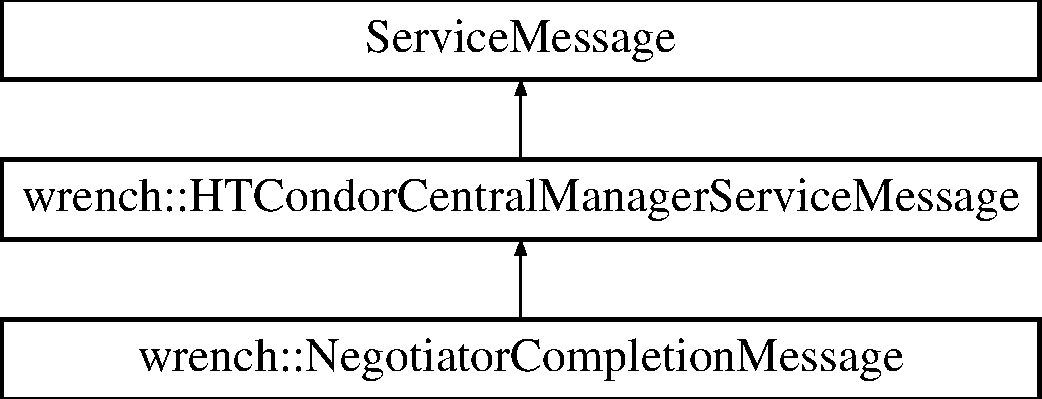
\includegraphics[height=4.000000cm]{classwrench_1_1_h_t_condor_central_manager_service_message}
\end{center}
\end{figure}
\subsection*{Protected Member Functions}
\begin{DoxyCompactItemize}
\item 
\hyperlink{classwrench_1_1_h_t_condor_central_manager_service_message_a18405b39184680404710905465d3a573}{H\+T\+Condor\+Central\+Manager\+Service\+Message} (std\+::string \hyperlink{classwrench_1_1_simulation_message_ab224f6dd8ec5ee2e7f65bfcdf2b8a86b}{name}, double \hyperlink{classwrench_1_1_simulation_message_a914f2732713f7c02898e66f05a7cb8a1}{payload})
\begin{DoxyCompactList}\small\item\em Constructor. \end{DoxyCompactList}\end{DoxyCompactItemize}
\subsection*{Additional Inherited Members}


\subsection{Constructor \& Destructor Documentation}
\mbox{\Hypertarget{classwrench_1_1_h_t_condor_central_manager_service_message_a18405b39184680404710905465d3a573}\label{classwrench_1_1_h_t_condor_central_manager_service_message_a18405b39184680404710905465d3a573}} 
\index{wrench\+::\+H\+T\+Condor\+Central\+Manager\+Service\+Message@{wrench\+::\+H\+T\+Condor\+Central\+Manager\+Service\+Message}!H\+T\+Condor\+Central\+Manager\+Service\+Message@{H\+T\+Condor\+Central\+Manager\+Service\+Message}}
\index{H\+T\+Condor\+Central\+Manager\+Service\+Message@{H\+T\+Condor\+Central\+Manager\+Service\+Message}!wrench\+::\+H\+T\+Condor\+Central\+Manager\+Service\+Message@{wrench\+::\+H\+T\+Condor\+Central\+Manager\+Service\+Message}}
\subsubsection{\texorpdfstring{H\+T\+Condor\+Central\+Manager\+Service\+Message()}{HTCondorCentralManagerServiceMessage()}}
{\footnotesize\ttfamily wrench\+::\+H\+T\+Condor\+Central\+Manager\+Service\+Message\+::\+H\+T\+Condor\+Central\+Manager\+Service\+Message (\begin{DoxyParamCaption}\item[{std\+::string}]{name,  }\item[{double}]{payload }\end{DoxyParamCaption})\hspace{0.3cm}{\ttfamily [protected]}}



Constructor. 


\begin{DoxyParams}{Parameters}
{\em name} & the message name \\
\hline
{\em payload} & the message size in bytes \\
\hline
\end{DoxyParams}


The documentation for this class was generated from the following files\+:\begin{DoxyCompactItemize}
\item 
/\+Users/rafsilva/\+Documents/isi/workspace/wrench/wrench/include/wrench/services/compute/htcondor/H\+T\+Condor\+Central\+Manager\+Service\+Message.\+h\item 
/\+Users/rafsilva/\+Documents/isi/workspace/wrench/wrench/src/wrench/services/compute/htcondor/H\+T\+Condor\+Central\+Manager\+Service\+Message.\+cpp\end{DoxyCompactItemize}

\hypertarget{classwrench_1_1_h_t_condor_central_manager_service_message_payload}{}\section{wrench\+:\+:H\+T\+Condor\+Central\+Manager\+Service\+Message\+Payload Class Reference}
\label{classwrench_1_1_h_t_condor_central_manager_service_message_payload}\index{wrench\+::\+H\+T\+Condor\+Central\+Manager\+Service\+Message\+Payload@{wrench\+::\+H\+T\+Condor\+Central\+Manager\+Service\+Message\+Payload}}


Configurable message payloads for an H\+T\+Condor Central Manager service.  




{\ttfamily \#include $<$H\+T\+Condor\+Central\+Manager\+Service\+Message\+Payload.\+h$>$}

Inheritance diagram for wrench\+:\+:H\+T\+Condor\+Central\+Manager\+Service\+Message\+Payload\+:\begin{figure}[H]
\begin{center}
\leavevmode
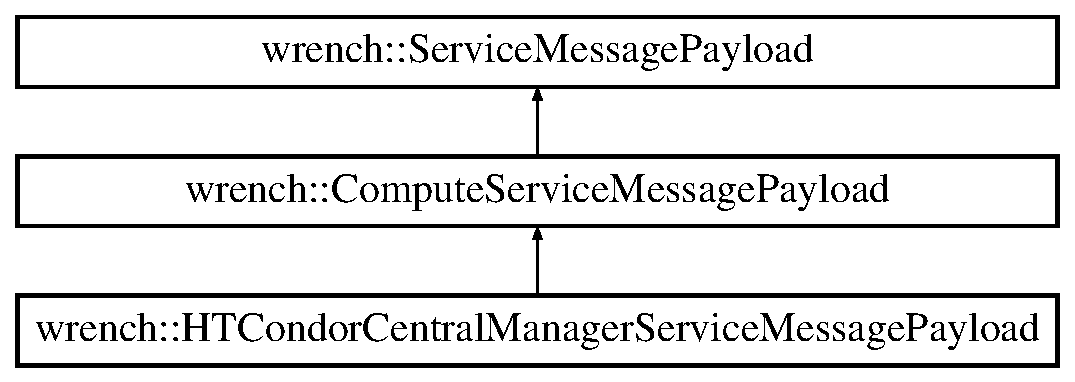
\includegraphics[height=3.000000cm]{classwrench_1_1_h_t_condor_central_manager_service_message_payload}
\end{center}
\end{figure}
\subsection*{Static Public Attributes}
\begin{DoxyCompactItemize}
\item 
\mbox{\Hypertarget{classwrench_1_1_h_t_condor_central_manager_service_message_payload_a7359fb0be37a14e6afb9efa9ec2d9c38}\label{classwrench_1_1_h_t_condor_central_manager_service_message_payload_a7359fb0be37a14e6afb9efa9ec2d9c38}} 
static const std\+::string \hyperlink{classwrench_1_1_h_t_condor_central_manager_service_message_payload_a7359fb0be37a14e6afb9efa9ec2d9c38}{H\+T\+C\+O\+N\+D\+O\+R\+\_\+\+N\+E\+G\+O\+T\+I\+A\+T\+O\+R\+\_\+\+D\+O\+N\+E\+\_\+\+M\+E\+S\+S\+A\+G\+E\+\_\+\+P\+A\+Y\+L\+O\+AD}
\begin{DoxyCompactList}\small\item\em The number of bytes in the control message sent by the daemon to state that the negotiator has been completed. \end{DoxyCompactList}\end{DoxyCompactItemize}


\subsection{Detailed Description}
Configurable message payloads for an H\+T\+Condor Central Manager service. 

The documentation for this class was generated from the following file\+:\begin{DoxyCompactItemize}
\item 
/\+Users/rafsilva/\+Documents/isi/workspace/wrench/wrench/include/wrench/services/compute/htcondor/H\+T\+Condor\+Central\+Manager\+Service\+Message\+Payload.\+h\end{DoxyCompactItemize}

\hypertarget{classwrench_1_1_h_t_condor_negotiator_service}{}\section{wrench\+:\+:H\+T\+Condor\+Negotiator\+Service Class Reference}
\label{classwrench_1_1_h_t_condor_negotiator_service}\index{wrench\+::\+H\+T\+Condor\+Negotiator\+Service@{wrench\+::\+H\+T\+Condor\+Negotiator\+Service}}
Inheritance diagram for wrench\+:\+:H\+T\+Condor\+Negotiator\+Service\+:\begin{figure}[H]
\begin{center}
\leavevmode
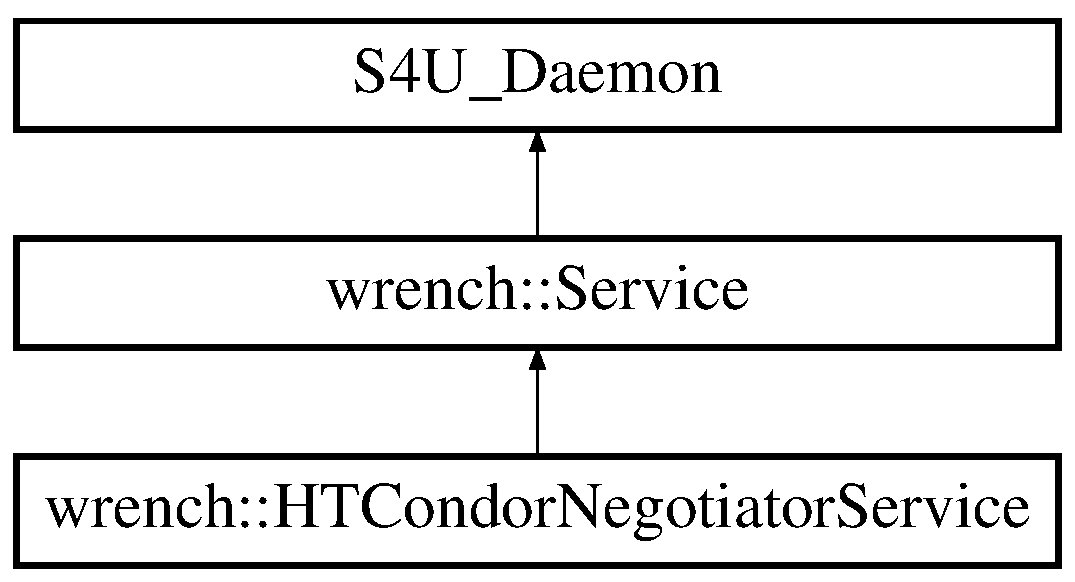
\includegraphics[height=3.000000cm]{classwrench_1_1_h_t_condor_negotiator_service}
\end{center}
\end{figure}
\subsection*{Public Member Functions}
\begin{DoxyCompactItemize}
\item 
\hyperlink{classwrench_1_1_h_t_condor_negotiator_service_a26a062744cd9445e3d77a984d794e53e}{H\+T\+Condor\+Negotiator\+Service} (std\+::string \&\hyperlink{classwrench_1_1_s4_u___daemon_a52bc0b9a6cd248310749dac086819f00}{hostname}, std\+::map$<$ \hyperlink{classwrench_1_1_compute_service}{Compute\+Service} $\ast$, unsigned long $>$ \&compute\+\_\+resources, std\+::map$<$ \hyperlink{classwrench_1_1_standard_job}{Standard\+Job} $\ast$, \hyperlink{classwrench_1_1_compute_service}{Compute\+Service} $\ast$$>$ \&running\+\_\+jobs, std\+::vector$<$ \hyperlink{classwrench_1_1_standard_job}{Standard\+Job} $\ast$$>$ \&pending\+\_\+jobs, std\+::string \&reply\+\_\+mailbox)
\begin{DoxyCompactList}\small\item\em Constructor. \end{DoxyCompactList}\item 
\mbox{\Hypertarget{classwrench_1_1_h_t_condor_negotiator_service_abbf969719d1b43ccfce10e7546eecea0}\label{classwrench_1_1_h_t_condor_negotiator_service_abbf969719d1b43ccfce10e7546eecea0}} 
\hyperlink{classwrench_1_1_h_t_condor_negotiator_service_abbf969719d1b43ccfce10e7546eecea0}{$\sim$\+H\+T\+Condor\+Negotiator\+Service} ()
\begin{DoxyCompactList}\small\item\em Destructor. \end{DoxyCompactList}\end{DoxyCompactItemize}
\subsection*{Additional Inherited Members}


\subsection{Constructor \& Destructor Documentation}
\mbox{\Hypertarget{classwrench_1_1_h_t_condor_negotiator_service_a26a062744cd9445e3d77a984d794e53e}\label{classwrench_1_1_h_t_condor_negotiator_service_a26a062744cd9445e3d77a984d794e53e}} 
\index{wrench\+::\+H\+T\+Condor\+Negotiator\+Service@{wrench\+::\+H\+T\+Condor\+Negotiator\+Service}!H\+T\+Condor\+Negotiator\+Service@{H\+T\+Condor\+Negotiator\+Service}}
\index{H\+T\+Condor\+Negotiator\+Service@{H\+T\+Condor\+Negotiator\+Service}!wrench\+::\+H\+T\+Condor\+Negotiator\+Service@{wrench\+::\+H\+T\+Condor\+Negotiator\+Service}}
\subsubsection{\texorpdfstring{H\+T\+Condor\+Negotiator\+Service()}{HTCondorNegotiatorService()}}
{\footnotesize\ttfamily wrench\+::\+H\+T\+Condor\+Negotiator\+Service\+::\+H\+T\+Condor\+Negotiator\+Service (\begin{DoxyParamCaption}\item[{std\+::string \&}]{hostname,  }\item[{std\+::map$<$ \hyperlink{classwrench_1_1_compute_service}{Compute\+Service} $\ast$, unsigned long $>$ \&}]{compute\+\_\+resources,  }\item[{std\+::map$<$ \hyperlink{classwrench_1_1_standard_job}{Standard\+Job} $\ast$, \hyperlink{classwrench_1_1_compute_service}{Compute\+Service} $\ast$$>$ \&}]{running\+\_\+jobs,  }\item[{std\+::vector$<$ \hyperlink{classwrench_1_1_standard_job}{Standard\+Job} $\ast$$>$ \&}]{pending\+\_\+jobs,  }\item[{std\+::string \&}]{reply\+\_\+mailbox }\end{DoxyParamCaption})}



Constructor. 


\begin{DoxyParams}{Parameters}
{\em hostname} & the hostname on which to start the service \\
\hline
{\em compute\+\_\+resources} & a set of compute resources available via the H\+T\+Condor pool \\
\hline
{\em running\+\_\+jobs} & \\
\hline
{\em pending\+\_\+jobs} & a list of pending jobs \\
\hline
{\em reply\+\_\+mailbox} & the mailbox to which the \char`\"{}done/failed\char`\"{} message should be sent \\
\hline
\end{DoxyParams}


The documentation for this class was generated from the following files\+:\begin{DoxyCompactItemize}
\item 
/\+Users/rafsilva/\+Documents/isi/workspace/wrench/wrench/include/wrench/services/compute/htcondor/H\+T\+Condor\+Negotiator\+Service.\+h\item 
/\+Users/rafsilva/\+Documents/isi/workspace/wrench/wrench/src/wrench/services/compute/htcondor/H\+T\+Condor\+Negotiator\+Service.\+cpp\end{DoxyCompactItemize}

\hypertarget{classwrench_1_1_h_t_condor_service}{}\section{wrench\+:\+:H\+T\+Condor\+Service Class Reference}
\label{classwrench_1_1_h_t_condor_service}\index{wrench\+::\+H\+T\+Condor\+Service@{wrench\+::\+H\+T\+Condor\+Service}}


A workload management framework compute service.  




{\ttfamily \#include $<$H\+T\+Condor\+Service.\+h$>$}

Inheritance diagram for wrench\+:\+:H\+T\+Condor\+Service\+:\begin{figure}[H]
\begin{center}
\leavevmode
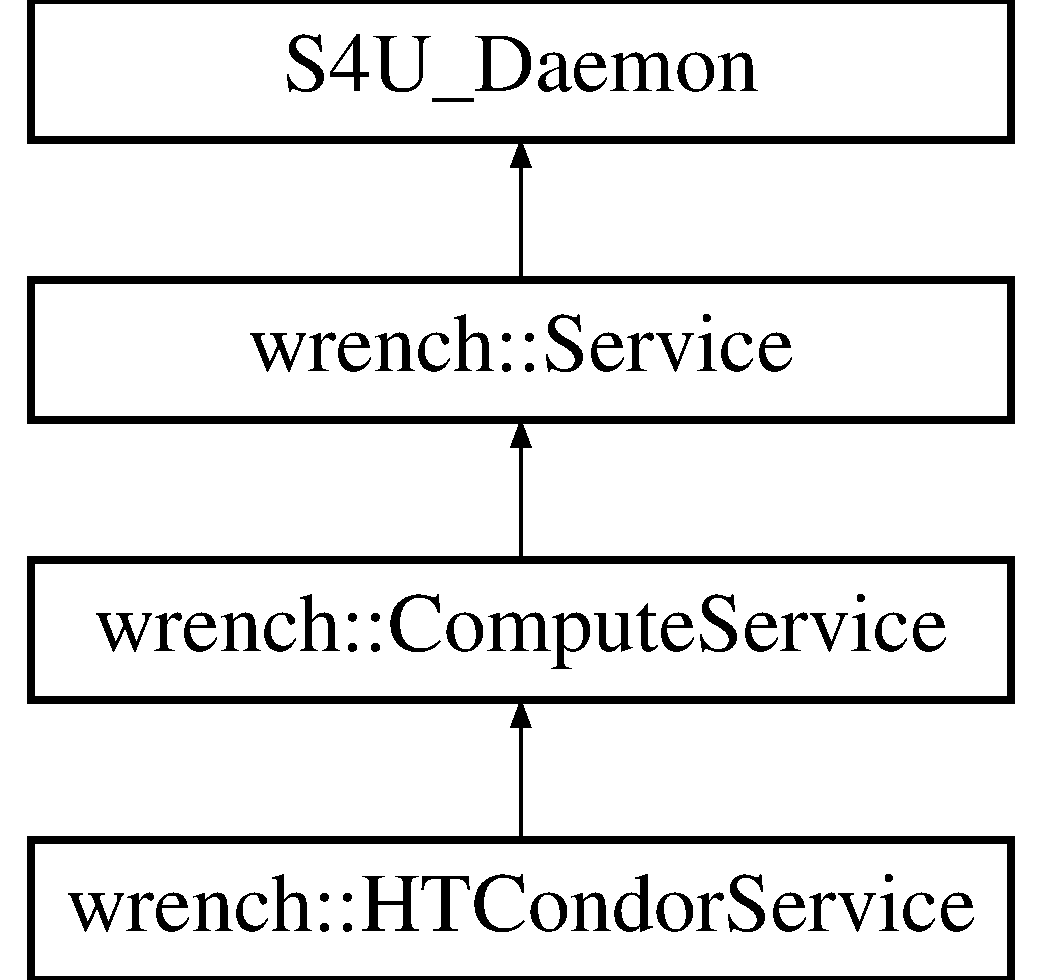
\includegraphics[height=4.000000cm]{classwrench_1_1_h_t_condor_service}
\end{center}
\end{figure}
\subsection*{Public Member Functions}
\begin{DoxyCompactItemize}
\item 
\hyperlink{classwrench_1_1_h_t_condor_service_a4632c26bb4c08757ac2ceeb57cd8e2d3}{H\+T\+Condor\+Service} (const std\+::string \&\hyperlink{classwrench_1_1_s4_u___daemon_a52bc0b9a6cd248310749dac086819f00}{hostname}, const std\+::string \&pool\+\_\+name, std\+::set$<$ \hyperlink{classwrench_1_1_compute_service}{Compute\+Service} $\ast$$>$ compute\+\_\+resources, std\+::map$<$ std\+::string, std\+::string $>$ \hyperlink{classwrench_1_1_service_a032143b1e2d7296dde9b4ca1e34845ce}{property\+\_\+list}=\{\}, std\+::map$<$ std\+::string, std\+::string $>$ \hyperlink{classwrench_1_1_service_a63865f20c92027ab626ab1347b0099d2}{messagepayload\+\_\+list}=\{\})
\begin{DoxyCompactList}\small\item\em Constructor. \end{DoxyCompactList}\item 
\mbox{\Hypertarget{classwrench_1_1_h_t_condor_service_a0b8eeb37bbbc61f3906266fc9d34d136}\label{classwrench_1_1_h_t_condor_service_a0b8eeb37bbbc61f3906266fc9d34d136}} 
\hyperlink{classwrench_1_1_h_t_condor_service_a0b8eeb37bbbc61f3906266fc9d34d136}{$\sim$\+H\+T\+Condor\+Service} () override
\begin{DoxyCompactList}\small\item\em Destructor. \end{DoxyCompactList}\item 
\hyperlink{classwrench_1_1_storage_service}{Storage\+Service} $\ast$ \hyperlink{classwrench_1_1_h_t_condor_service_a4c8a4111afff9952e90d210a8b0bdf35}{get\+Local\+Storage\+Service} () const
\item 
\mbox{\Hypertarget{classwrench_1_1_h_t_condor_service_a21750683c0445a8d208ef3862a2cea21}\label{classwrench_1_1_h_t_condor_service_a21750683c0445a8d208ef3862a2cea21}} 
void {\bfseries set\+Local\+Storage\+Service} (\hyperlink{classwrench_1_1_storage_service}{Storage\+Service} $\ast$local\+\_\+storage\+\_\+service)
\item 
void \hyperlink{classwrench_1_1_h_t_condor_service_a1fac4517c82ac0b0737cd6ca75bba952}{submit\+Pilot\+Job} (\hyperlink{classwrench_1_1_pilot_job}{Pilot\+Job} $\ast$job, std\+::map$<$ std\+::string, std\+::string $>$ \&service\+\_\+specific\+\_\+arguments) override
\begin{DoxyCompactList}\small\item\em Asynchronously submit a pilot job to the cloud service. \end{DoxyCompactList}\item 
void \hyperlink{classwrench_1_1_h_t_condor_service_a686a511797b0d6250e7d22941c427ef3}{submit\+Standard\+Job} (\hyperlink{classwrench_1_1_standard_job}{Standard\+Job} $\ast$job, std\+::map$<$ std\+::string, std\+::string $>$ \&service\+\_\+specific\+\_\+arguments) override
\begin{DoxyCompactList}\small\item\em Submit a standard job to the H\+T\+Condor service. \end{DoxyCompactList}\item 
void \hyperlink{classwrench_1_1_h_t_condor_service_a5e502916770f5d7e899bf1c106557fbc}{terminate\+Pilot\+Job} (\hyperlink{classwrench_1_1_pilot_job}{Pilot\+Job} $\ast$job) override
\begin{DoxyCompactList}\small\item\em Terminate a pilot job to the compute service. \end{DoxyCompactList}\item 
void \hyperlink{classwrench_1_1_h_t_condor_service_a23ba6cd749a7d90ce153038c606610a3}{terminate\+Standard\+Job} (\hyperlink{classwrench_1_1_standard_job}{Standard\+Job} $\ast$job) override
\begin{DoxyCompactList}\small\item\em Terminate a standard job to the compute service (virtual) \end{DoxyCompactList}\end{DoxyCompactItemize}
\subsection*{Additional Inherited Members}


\subsection{Detailed Description}
A workload management framework compute service. 

\subsection{Constructor \& Destructor Documentation}
\mbox{\Hypertarget{classwrench_1_1_h_t_condor_service_a4632c26bb4c08757ac2ceeb57cd8e2d3}\label{classwrench_1_1_h_t_condor_service_a4632c26bb4c08757ac2ceeb57cd8e2d3}} 
\index{wrench\+::\+H\+T\+Condor\+Service@{wrench\+::\+H\+T\+Condor\+Service}!H\+T\+Condor\+Service@{H\+T\+Condor\+Service}}
\index{H\+T\+Condor\+Service@{H\+T\+Condor\+Service}!wrench\+::\+H\+T\+Condor\+Service@{wrench\+::\+H\+T\+Condor\+Service}}
\subsubsection{\texorpdfstring{H\+T\+Condor\+Service()}{HTCondorService()}}
{\footnotesize\ttfamily wrench\+::\+H\+T\+Condor\+Service\+::\+H\+T\+Condor\+Service (\begin{DoxyParamCaption}\item[{const std\+::string \&}]{hostname,  }\item[{const std\+::string \&}]{pool\+\_\+name,  }\item[{std\+::set$<$ \hyperlink{classwrench_1_1_compute_service}{Compute\+Service} $\ast$$>$}]{compute\+\_\+resources,  }\item[{std\+::map$<$ std\+::string, std\+::string $>$}]{property\+\_\+list = {\ttfamily \{\}},  }\item[{std\+::map$<$ std\+::string, std\+::string $>$}]{messagepayload\+\_\+list = {\ttfamily \{\}} }\end{DoxyParamCaption})}



Constructor. 


\begin{DoxyParams}{Parameters}
{\em hostname} & the hostname on which to start the service \\
\hline
{\em pool\+\_\+name} & H\+T\+Condor pool name \\
\hline
{\em compute\+\_\+resources} & a set of compute resources available via the H\+T\+Condor pool \\
\hline
{\em property\+\_\+list} & a property list (\{\} means \char`\"{}use all defaults\char`\"{}) \\
\hline
{\em messagepayload\+\_\+list} & a message payload list (\{\} means \char`\"{}use all defaults\char`\"{})\\
\hline
\end{DoxyParams}

\begin{DoxyExceptions}{Exceptions}
{\em std\+::runtime\+\_\+error} & \\
\hline
\end{DoxyExceptions}


\subsection{Member Function Documentation}
\mbox{\Hypertarget{classwrench_1_1_h_t_condor_service_a4c8a4111afff9952e90d210a8b0bdf35}\label{classwrench_1_1_h_t_condor_service_a4c8a4111afff9952e90d210a8b0bdf35}} 
\index{wrench\+::\+H\+T\+Condor\+Service@{wrench\+::\+H\+T\+Condor\+Service}!get\+Local\+Storage\+Service@{get\+Local\+Storage\+Service}}
\index{get\+Local\+Storage\+Service@{get\+Local\+Storage\+Service}!wrench\+::\+H\+T\+Condor\+Service@{wrench\+::\+H\+T\+Condor\+Service}}
\subsubsection{\texorpdfstring{get\+Local\+Storage\+Service()}{getLocalStorageService()}}
{\footnotesize\ttfamily \hyperlink{classwrench_1_1_storage_service}{Storage\+Service} $\ast$ wrench\+::\+H\+T\+Condor\+Service\+::get\+Local\+Storage\+Service (\begin{DoxyParamCaption}{ }\end{DoxyParamCaption}) const}

Get a pointer to the service local \hyperlink{classwrench_1_1_storage_service}{Storage\+Service} object \begin{DoxyReturn}{Returns}
a pointer to the service local \hyperlink{classwrench_1_1_storage_service}{Storage\+Service} object 
\end{DoxyReturn}
\mbox{\Hypertarget{classwrench_1_1_h_t_condor_service_a1fac4517c82ac0b0737cd6ca75bba952}\label{classwrench_1_1_h_t_condor_service_a1fac4517c82ac0b0737cd6ca75bba952}} 
\index{wrench\+::\+H\+T\+Condor\+Service@{wrench\+::\+H\+T\+Condor\+Service}!submit\+Pilot\+Job@{submit\+Pilot\+Job}}
\index{submit\+Pilot\+Job@{submit\+Pilot\+Job}!wrench\+::\+H\+T\+Condor\+Service@{wrench\+::\+H\+T\+Condor\+Service}}
\subsubsection{\texorpdfstring{submit\+Pilot\+Job()}{submitPilotJob()}}
{\footnotesize\ttfamily void wrench\+::\+H\+T\+Condor\+Service\+::submit\+Pilot\+Job (\begin{DoxyParamCaption}\item[{\hyperlink{classwrench_1_1_pilot_job}{Pilot\+Job} $\ast$}]{job,  }\item[{std\+::map$<$ std\+::string, std\+::string $>$ \&}]{service\+\_\+specific\+\_\+args }\end{DoxyParamCaption})\hspace{0.3cm}{\ttfamily [override]}, {\ttfamily [virtual]}}



Asynchronously submit a pilot job to the cloud service. 


\begin{DoxyParams}{Parameters}
{\em job} & a pilot job \\
\hline
{\em service\+\_\+specific\+\_\+args} & service specific arguments\\
\hline
\end{DoxyParams}

\begin{DoxyExceptions}{Exceptions}
{\em \hyperlink{classwrench_1_1_workflow_execution_exception}{Workflow\+Execution\+Exception}} & \\
\hline
{\em std\+::runtime\+\_\+error} & \\
\hline
\end{DoxyExceptions}


Implements \hyperlink{classwrench_1_1_compute_service}{wrench\+::\+Compute\+Service}.

\mbox{\Hypertarget{classwrench_1_1_h_t_condor_service_a686a511797b0d6250e7d22941c427ef3}\label{classwrench_1_1_h_t_condor_service_a686a511797b0d6250e7d22941c427ef3}} 
\index{wrench\+::\+H\+T\+Condor\+Service@{wrench\+::\+H\+T\+Condor\+Service}!submit\+Standard\+Job@{submit\+Standard\+Job}}
\index{submit\+Standard\+Job@{submit\+Standard\+Job}!wrench\+::\+H\+T\+Condor\+Service@{wrench\+::\+H\+T\+Condor\+Service}}
\subsubsection{\texorpdfstring{submit\+Standard\+Job()}{submitStandardJob()}}
{\footnotesize\ttfamily void wrench\+::\+H\+T\+Condor\+Service\+::submit\+Standard\+Job (\begin{DoxyParamCaption}\item[{\hyperlink{classwrench_1_1_standard_job}{Standard\+Job} $\ast$}]{job,  }\item[{std\+::map$<$ std\+::string, std\+::string $>$ \&}]{service\+\_\+specific\+\_\+args }\end{DoxyParamCaption})\hspace{0.3cm}{\ttfamily [override]}, {\ttfamily [virtual]}}



Submit a standard job to the H\+T\+Condor service. 


\begin{DoxyParams}{Parameters}
{\em job} & a standard job \\
\hline
{\em service\+\_\+specific\+\_\+args} & service specific arguments\\
\hline
\end{DoxyParams}

\begin{DoxyExceptions}{Exceptions}
{\em \hyperlink{classwrench_1_1_workflow_execution_exception}{Workflow\+Execution\+Exception}} & \\
\hline
{\em std\+::runtime\+\_\+error} & \\
\hline
\end{DoxyExceptions}


Implements \hyperlink{classwrench_1_1_compute_service}{wrench\+::\+Compute\+Service}.

\mbox{\Hypertarget{classwrench_1_1_h_t_condor_service_a5e502916770f5d7e899bf1c106557fbc}\label{classwrench_1_1_h_t_condor_service_a5e502916770f5d7e899bf1c106557fbc}} 
\index{wrench\+::\+H\+T\+Condor\+Service@{wrench\+::\+H\+T\+Condor\+Service}!terminate\+Pilot\+Job@{terminate\+Pilot\+Job}}
\index{terminate\+Pilot\+Job@{terminate\+Pilot\+Job}!wrench\+::\+H\+T\+Condor\+Service@{wrench\+::\+H\+T\+Condor\+Service}}
\subsubsection{\texorpdfstring{terminate\+Pilot\+Job()}{terminatePilotJob()}}
{\footnotesize\ttfamily void wrench\+::\+H\+T\+Condor\+Service\+::terminate\+Pilot\+Job (\begin{DoxyParamCaption}\item[{\hyperlink{classwrench_1_1_pilot_job}{Pilot\+Job} $\ast$}]{job }\end{DoxyParamCaption})\hspace{0.3cm}{\ttfamily [override]}, {\ttfamily [virtual]}}



Terminate a pilot job to the compute service. 


\begin{DoxyParams}{Parameters}
{\em job} & the job\\
\hline
\end{DoxyParams}

\begin{DoxyExceptions}{Exceptions}
{\em std\+::runtime\+\_\+error} & \\
\hline
\end{DoxyExceptions}


Implements \hyperlink{classwrench_1_1_compute_service}{wrench\+::\+Compute\+Service}.

\mbox{\Hypertarget{classwrench_1_1_h_t_condor_service_a23ba6cd749a7d90ce153038c606610a3}\label{classwrench_1_1_h_t_condor_service_a23ba6cd749a7d90ce153038c606610a3}} 
\index{wrench\+::\+H\+T\+Condor\+Service@{wrench\+::\+H\+T\+Condor\+Service}!terminate\+Standard\+Job@{terminate\+Standard\+Job}}
\index{terminate\+Standard\+Job@{terminate\+Standard\+Job}!wrench\+::\+H\+T\+Condor\+Service@{wrench\+::\+H\+T\+Condor\+Service}}
\subsubsection{\texorpdfstring{terminate\+Standard\+Job()}{terminateStandardJob()}}
{\footnotesize\ttfamily void wrench\+::\+H\+T\+Condor\+Service\+::terminate\+Standard\+Job (\begin{DoxyParamCaption}\item[{\hyperlink{classwrench_1_1_standard_job}{Standard\+Job} $\ast$}]{job }\end{DoxyParamCaption})\hspace{0.3cm}{\ttfamily [override]}, {\ttfamily [virtual]}}



Terminate a standard job to the compute service (virtual) 


\begin{DoxyParams}{Parameters}
{\em job} & the job\\
\hline
\end{DoxyParams}

\begin{DoxyExceptions}{Exceptions}
{\em std\+::runtime\+\_\+error} & \\
\hline
\end{DoxyExceptions}


Implements \hyperlink{classwrench_1_1_compute_service}{wrench\+::\+Compute\+Service}.



The documentation for this class was generated from the following files\+:\begin{DoxyCompactItemize}
\item 
/\+Users/rafsilva/\+Documents/isi/workspace/wrench/wrench/include/wrench/services/compute/htcondor/H\+T\+Condor\+Service.\+h\item 
/\+Users/rafsilva/\+Documents/isi/workspace/wrench/wrench/src/wrench/services/compute/htcondor/H\+T\+Condor\+Service.\+cpp\end{DoxyCompactItemize}

\hypertarget{classwrench_1_1_h_t_condor_service_message_payload}{}\section{wrench\+:\+:H\+T\+Condor\+Service\+Message\+Payload Class Reference}
\label{classwrench_1_1_h_t_condor_service_message_payload}\index{wrench\+::\+H\+T\+Condor\+Service\+Message\+Payload@{wrench\+::\+H\+T\+Condor\+Service\+Message\+Payload}}


Configurable message payloads for an \hyperlink{classwrench_1_1_h_t_condor_service}{H\+T\+Condor\+Service}.  




{\ttfamily \#include $<$H\+T\+Condor\+Service\+Message\+Payload.\+h$>$}

Inheritance diagram for wrench\+:\+:H\+T\+Condor\+Service\+Message\+Payload\+:\begin{figure}[H]
\begin{center}
\leavevmode
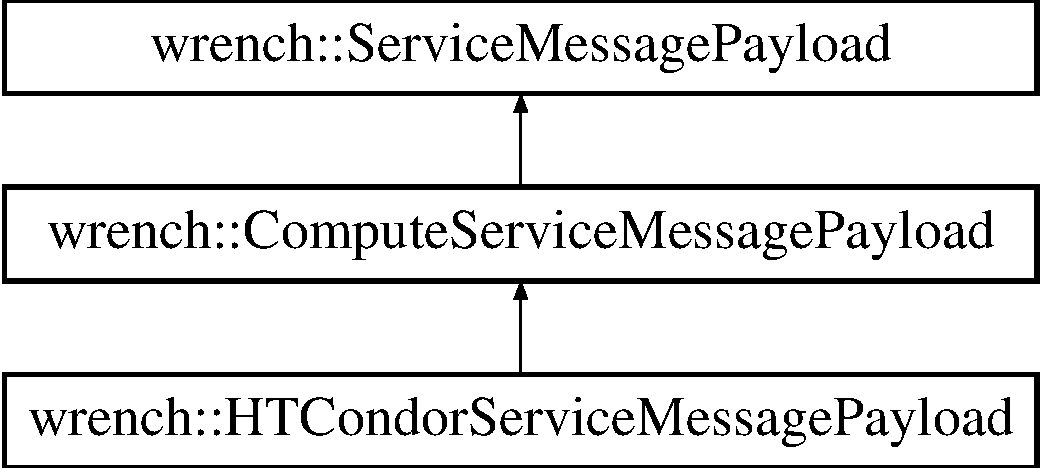
\includegraphics[height=3.000000cm]{classwrench_1_1_h_t_condor_service_message_payload}
\end{center}
\end{figure}
\subsection*{Additional Inherited Members}


\subsection{Detailed Description}
Configurable message payloads for an \hyperlink{classwrench_1_1_h_t_condor_service}{H\+T\+Condor\+Service}. 

The documentation for this class was generated from the following file\+:\begin{DoxyCompactItemize}
\item 
/\+Users/rafsilva/\+Documents/isi/workspace/wrench/wrench/include/wrench/services/compute/htcondor/H\+T\+Condor\+Service\+Message\+Payload.\+h\end{DoxyCompactItemize}

\hypertarget{classwrench_1_1_h_t_condor_service_property}{}\section{wrench\+:\+:H\+T\+Condor\+Service\+Property Class Reference}
\label{classwrench_1_1_h_t_condor_service_property}\index{wrench\+::\+H\+T\+Condor\+Service\+Property@{wrench\+::\+H\+T\+Condor\+Service\+Property}}


Properties for an H\+T\+Condor service.  




{\ttfamily \#include $<$H\+T\+Condor\+Service\+Property.\+h$>$}

Inheritance diagram for wrench\+:\+:H\+T\+Condor\+Service\+Property\+:\begin{figure}[H]
\begin{center}
\leavevmode
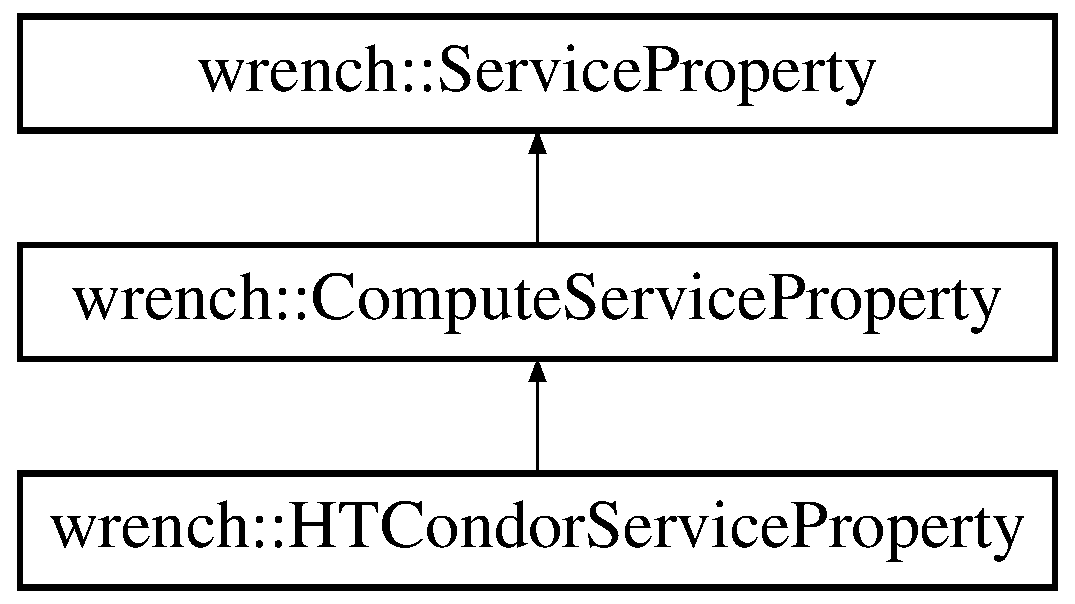
\includegraphics[height=3.000000cm]{classwrench_1_1_h_t_condor_service_property}
\end{center}
\end{figure}
\subsection*{Additional Inherited Members}


\subsection{Detailed Description}
Properties for an H\+T\+Condor service. 

The documentation for this class was generated from the following file\+:\begin{DoxyCompactItemize}
\item 
/\+Users/rafsilva/\+Documents/isi/workspace/wrench/wrench/include/wrench/services/compute/htcondor/H\+T\+Condor\+Service\+Property.\+h\end{DoxyCompactItemize}

\hypertarget{classwrench_1_1_job_cannot_be_forgotten}{}\section{wrench\+:\+:Job\+Cannot\+Be\+Forgotten Class Reference}
\label{classwrench_1_1_job_cannot_be_forgotten}\index{wrench\+::\+Job\+Cannot\+Be\+Forgotten@{wrench\+::\+Job\+Cannot\+Be\+Forgotten}}


A \char`\"{}job cannot be forgotten\char`\"{} failure cause.  




{\ttfamily \#include $<$Failure\+Cause.\+h$>$}

Inheritance diagram for wrench\+:\+:Job\+Cannot\+Be\+Forgotten\+:\begin{figure}[H]
\begin{center}
\leavevmode
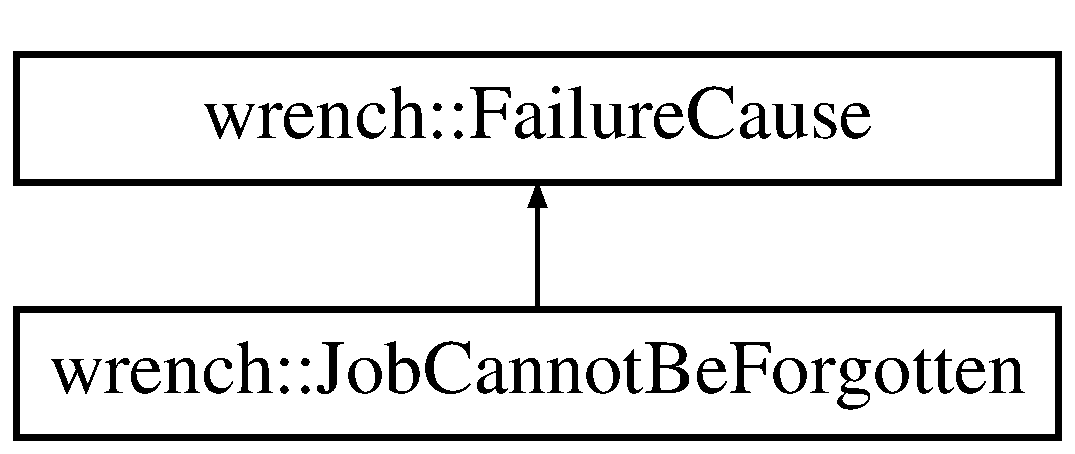
\includegraphics[height=2.000000cm]{classwrench_1_1_job_cannot_be_forgotten}
\end{center}
\end{figure}
\subsection*{Public Member Functions}
\begin{DoxyCompactItemize}
\item 
\hyperlink{classwrench_1_1_workflow_job}{Workflow\+Job} $\ast$ \hyperlink{classwrench_1_1_job_cannot_be_forgotten_ae21aa5adc48ff0998d9fefc7f2c4c9f9}{get\+Job} ()
\begin{DoxyCompactList}\small\item\em Getter. \end{DoxyCompactList}\item 
std\+::string \hyperlink{classwrench_1_1_job_cannot_be_forgotten_abbfbece144c738c9948bf8f01d6bbd53}{to\+String} ()
\begin{DoxyCompactList}\small\item\em Get the human-\/readable failure message. \end{DoxyCompactList}\end{DoxyCompactItemize}
\subsection*{Additional Inherited Members}


\subsection{Detailed Description}
A \char`\"{}job cannot be forgotten\char`\"{} failure cause. 

\subsection{Member Function Documentation}
\mbox{\Hypertarget{classwrench_1_1_job_cannot_be_forgotten_ae21aa5adc48ff0998d9fefc7f2c4c9f9}\label{classwrench_1_1_job_cannot_be_forgotten_ae21aa5adc48ff0998d9fefc7f2c4c9f9}} 
\index{wrench\+::\+Job\+Cannot\+Be\+Forgotten@{wrench\+::\+Job\+Cannot\+Be\+Forgotten}!get\+Job@{get\+Job}}
\index{get\+Job@{get\+Job}!wrench\+::\+Job\+Cannot\+Be\+Forgotten@{wrench\+::\+Job\+Cannot\+Be\+Forgotten}}
\subsubsection{\texorpdfstring{get\+Job()}{getJob()}}
{\footnotesize\ttfamily \hyperlink{classwrench_1_1_workflow_job}{Workflow\+Job} $\ast$ wrench\+::\+Job\+Cannot\+Be\+Forgotten\+::get\+Job (\begin{DoxyParamCaption}{ }\end{DoxyParamCaption})}



Getter. 

\begin{DoxyReturn}{Returns}
the job 
\end{DoxyReturn}
\mbox{\Hypertarget{classwrench_1_1_job_cannot_be_forgotten_abbfbece144c738c9948bf8f01d6bbd53}\label{classwrench_1_1_job_cannot_be_forgotten_abbfbece144c738c9948bf8f01d6bbd53}} 
\index{wrench\+::\+Job\+Cannot\+Be\+Forgotten@{wrench\+::\+Job\+Cannot\+Be\+Forgotten}!to\+String@{to\+String}}
\index{to\+String@{to\+String}!wrench\+::\+Job\+Cannot\+Be\+Forgotten@{wrench\+::\+Job\+Cannot\+Be\+Forgotten}}
\subsubsection{\texorpdfstring{to\+String()}{toString()}}
{\footnotesize\ttfamily std\+::string wrench\+::\+Job\+Cannot\+Be\+Forgotten\+::to\+String (\begin{DoxyParamCaption}{ }\end{DoxyParamCaption})\hspace{0.3cm}{\ttfamily [virtual]}}



Get the human-\/readable failure message. 

\begin{DoxyReturn}{Returns}
the message 
\end{DoxyReturn}


Implements \hyperlink{classwrench_1_1_failure_cause_afbad248ebe902409f2cd4f1d6f2b867d}{wrench\+::\+Failure\+Cause}.



The documentation for this class was generated from the following files\+:\begin{DoxyCompactItemize}
\item 
/\+Users/rafsilva/\+Documents/isi/workspace/wrench/wrench/include/wrench/workflow/execution\+\_\+events/Failure\+Cause.\+h\item 
/\+Users/rafsilva/\+Documents/isi/workspace/wrench/wrench/src/wrench/workflow/execution\+\_\+events/Failure\+Cause.\+cpp\end{DoxyCompactItemize}

\hypertarget{classwrench_1_1_job_cannot_be_terminated}{}\section{wrench\+:\+:Job\+Cannot\+Be\+Terminated Class Reference}
\label{classwrench_1_1_job_cannot_be_terminated}\index{wrench\+::\+Job\+Cannot\+Be\+Terminated@{wrench\+::\+Job\+Cannot\+Be\+Terminated}}


A \char`\"{}job cannot be terminated\char`\"{} failure cause.  




{\ttfamily \#include $<$Failure\+Cause.\+h$>$}

Inheritance diagram for wrench\+:\+:Job\+Cannot\+Be\+Terminated\+:\begin{figure}[H]
\begin{center}
\leavevmode
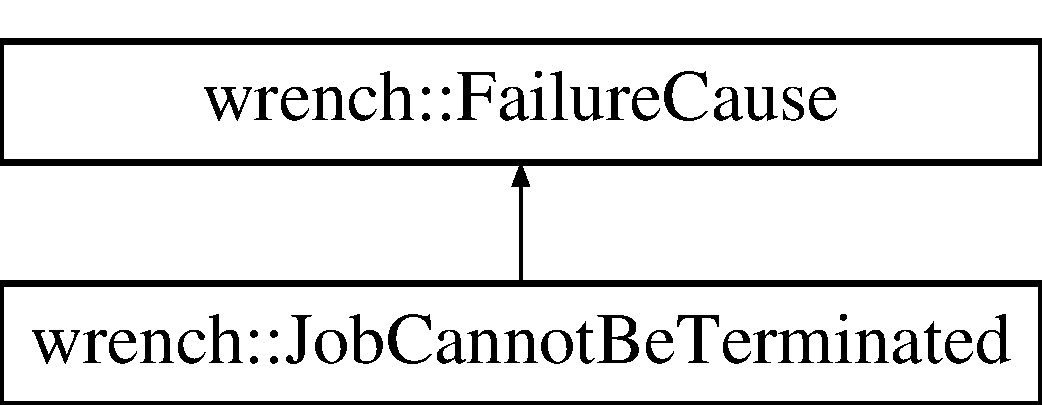
\includegraphics[height=2.000000cm]{classwrench_1_1_job_cannot_be_terminated}
\end{center}
\end{figure}
\subsection*{Public Member Functions}
\begin{DoxyCompactItemize}
\item 
\hyperlink{classwrench_1_1_workflow_job}{Workflow\+Job} $\ast$ \hyperlink{classwrench_1_1_job_cannot_be_terminated_af97232722e1b4feed0c12b9e0ced666f}{get\+Job} ()
\begin{DoxyCompactList}\small\item\em Getter. \end{DoxyCompactList}\item 
std\+::string \hyperlink{classwrench_1_1_job_cannot_be_terminated_acfa2b83db93bb68e0e773cc8b4a45505}{to\+String} ()
\begin{DoxyCompactList}\small\item\em Get the human-\/readable failure message. \end{DoxyCompactList}\end{DoxyCompactItemize}
\subsection*{Additional Inherited Members}


\subsection{Detailed Description}
A \char`\"{}job cannot be terminated\char`\"{} failure cause. 

\subsection{Member Function Documentation}
\mbox{\Hypertarget{classwrench_1_1_job_cannot_be_terminated_af97232722e1b4feed0c12b9e0ced666f}\label{classwrench_1_1_job_cannot_be_terminated_af97232722e1b4feed0c12b9e0ced666f}} 
\index{wrench\+::\+Job\+Cannot\+Be\+Terminated@{wrench\+::\+Job\+Cannot\+Be\+Terminated}!get\+Job@{get\+Job}}
\index{get\+Job@{get\+Job}!wrench\+::\+Job\+Cannot\+Be\+Terminated@{wrench\+::\+Job\+Cannot\+Be\+Terminated}}
\subsubsection{\texorpdfstring{get\+Job()}{getJob()}}
{\footnotesize\ttfamily \hyperlink{classwrench_1_1_workflow_job}{Workflow\+Job} $\ast$ wrench\+::\+Job\+Cannot\+Be\+Terminated\+::get\+Job (\begin{DoxyParamCaption}{ }\end{DoxyParamCaption})}



Getter. 

\begin{DoxyReturn}{Returns}
the job 
\end{DoxyReturn}
\mbox{\Hypertarget{classwrench_1_1_job_cannot_be_terminated_acfa2b83db93bb68e0e773cc8b4a45505}\label{classwrench_1_1_job_cannot_be_terminated_acfa2b83db93bb68e0e773cc8b4a45505}} 
\index{wrench\+::\+Job\+Cannot\+Be\+Terminated@{wrench\+::\+Job\+Cannot\+Be\+Terminated}!to\+String@{to\+String}}
\index{to\+String@{to\+String}!wrench\+::\+Job\+Cannot\+Be\+Terminated@{wrench\+::\+Job\+Cannot\+Be\+Terminated}}
\subsubsection{\texorpdfstring{to\+String()}{toString()}}
{\footnotesize\ttfamily std\+::string wrench\+::\+Job\+Cannot\+Be\+Terminated\+::to\+String (\begin{DoxyParamCaption}{ }\end{DoxyParamCaption})\hspace{0.3cm}{\ttfamily [virtual]}}



Get the human-\/readable failure message. 

\begin{DoxyReturn}{Returns}
the message 
\end{DoxyReturn}


Implements \hyperlink{classwrench_1_1_failure_cause_afbad248ebe902409f2cd4f1d6f2b867d}{wrench\+::\+Failure\+Cause}.



The documentation for this class was generated from the following files\+:\begin{DoxyCompactItemize}
\item 
/\+Users/rafsilva/\+Documents/isi/workspace/wrench/wrench/include/wrench/workflow/execution\+\_\+events/Failure\+Cause.\+h\item 
/\+Users/rafsilva/\+Documents/isi/workspace/wrench/wrench/src/wrench/workflow/execution\+\_\+events/Failure\+Cause.\+cpp\end{DoxyCompactItemize}

\hypertarget{classwrench_1_1_job_killed}{}\section{wrench\+:\+:Job\+Killed Class Reference}
\label{classwrench_1_1_job_killed}\index{wrench\+::\+Job\+Killed@{wrench\+::\+Job\+Killed}}


A \char`\"{}job has been killed\char`\"{} failure cause.  




{\ttfamily \#include $<$Failure\+Cause.\+h$>$}

Inheritance diagram for wrench\+:\+:Job\+Killed\+:\begin{figure}[H]
\begin{center}
\leavevmode
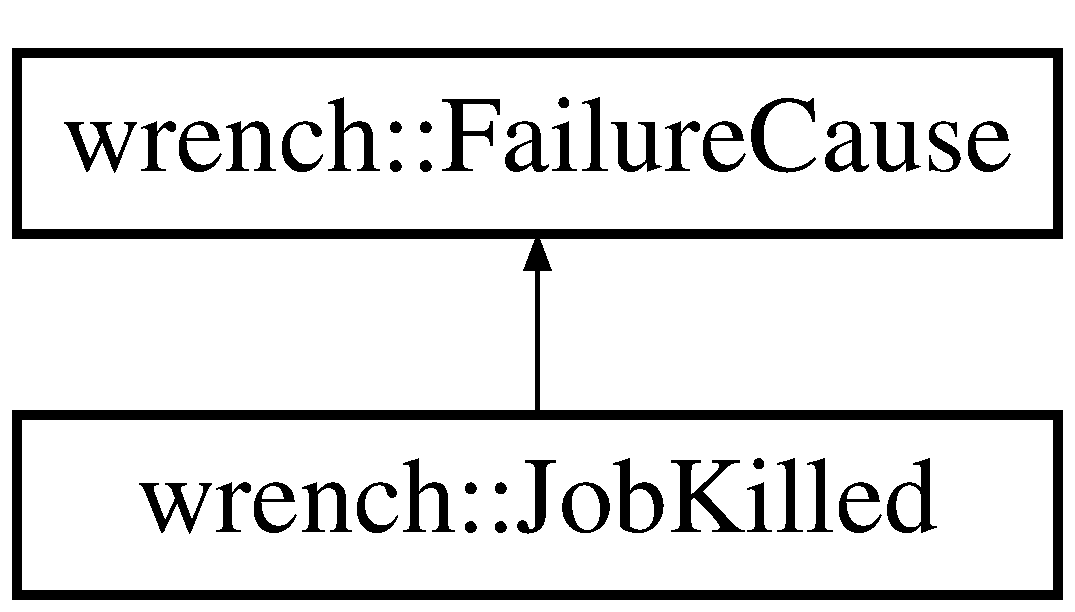
\includegraphics[height=2.000000cm]{classwrench_1_1_job_killed}
\end{center}
\end{figure}
\subsection*{Public Member Functions}
\begin{DoxyCompactItemize}
\item 
\hyperlink{classwrench_1_1_compute_service}{Compute\+Service} $\ast$ \hyperlink{classwrench_1_1_job_killed_a448c858885b28a03399103494ad85e5b}{get\+Compute\+Service} ()
\begin{DoxyCompactList}\small\item\em Getter. \end{DoxyCompactList}\item 
\hyperlink{classwrench_1_1_workflow_job}{Workflow\+Job} $\ast$ \hyperlink{classwrench_1_1_job_killed_a12b56e54f07217a9b0a3f3f67b001132}{get\+Job} ()
\begin{DoxyCompactList}\small\item\em Getter. \end{DoxyCompactList}\item 
std\+::string \hyperlink{classwrench_1_1_job_killed_aa9c6b749d16db4a313ffdd83629f1c76}{to\+String} ()
\begin{DoxyCompactList}\small\item\em Get the human-\/readable failure message. \end{DoxyCompactList}\end{DoxyCompactItemize}
\subsection*{Additional Inherited Members}


\subsection{Detailed Description}
A \char`\"{}job has been killed\char`\"{} failure cause. 

\subsection{Member Function Documentation}
\mbox{\Hypertarget{classwrench_1_1_job_killed_a448c858885b28a03399103494ad85e5b}\label{classwrench_1_1_job_killed_a448c858885b28a03399103494ad85e5b}} 
\index{wrench\+::\+Job\+Killed@{wrench\+::\+Job\+Killed}!get\+Compute\+Service@{get\+Compute\+Service}}
\index{get\+Compute\+Service@{get\+Compute\+Service}!wrench\+::\+Job\+Killed@{wrench\+::\+Job\+Killed}}
\subsubsection{\texorpdfstring{get\+Compute\+Service()}{getComputeService()}}
{\footnotesize\ttfamily \hyperlink{classwrench_1_1_compute_service}{Compute\+Service} $\ast$ wrench\+::\+Job\+Killed\+::get\+Compute\+Service (\begin{DoxyParamCaption}{ }\end{DoxyParamCaption})}



Getter. 

\begin{DoxyReturn}{Returns}
the compute service 
\end{DoxyReturn}
\mbox{\Hypertarget{classwrench_1_1_job_killed_a12b56e54f07217a9b0a3f3f67b001132}\label{classwrench_1_1_job_killed_a12b56e54f07217a9b0a3f3f67b001132}} 
\index{wrench\+::\+Job\+Killed@{wrench\+::\+Job\+Killed}!get\+Job@{get\+Job}}
\index{get\+Job@{get\+Job}!wrench\+::\+Job\+Killed@{wrench\+::\+Job\+Killed}}
\subsubsection{\texorpdfstring{get\+Job()}{getJob()}}
{\footnotesize\ttfamily \hyperlink{classwrench_1_1_workflow_job}{Workflow\+Job} $\ast$ wrench\+::\+Job\+Killed\+::get\+Job (\begin{DoxyParamCaption}{ }\end{DoxyParamCaption})}



Getter. 

\begin{DoxyReturn}{Returns}
the job 
\end{DoxyReturn}
\mbox{\Hypertarget{classwrench_1_1_job_killed_aa9c6b749d16db4a313ffdd83629f1c76}\label{classwrench_1_1_job_killed_aa9c6b749d16db4a313ffdd83629f1c76}} 
\index{wrench\+::\+Job\+Killed@{wrench\+::\+Job\+Killed}!to\+String@{to\+String}}
\index{to\+String@{to\+String}!wrench\+::\+Job\+Killed@{wrench\+::\+Job\+Killed}}
\subsubsection{\texorpdfstring{to\+String()}{toString()}}
{\footnotesize\ttfamily std\+::string wrench\+::\+Job\+Killed\+::to\+String (\begin{DoxyParamCaption}{ }\end{DoxyParamCaption})\hspace{0.3cm}{\ttfamily [virtual]}}



Get the human-\/readable failure message. 

\begin{DoxyReturn}{Returns}
the message 
\end{DoxyReturn}


Implements \hyperlink{classwrench_1_1_failure_cause_afbad248ebe902409f2cd4f1d6f2b867d}{wrench\+::\+Failure\+Cause}.



The documentation for this class was generated from the following files\+:\begin{DoxyCompactItemize}
\item 
/\+Users/rafsilva/\+Documents/isi/workspace/wrench/wrench/include/wrench/workflow/execution\+\_\+events/Failure\+Cause.\+h\item 
/\+Users/rafsilva/\+Documents/isi/workspace/wrench/wrench/src/wrench/workflow/execution\+\_\+events/Failure\+Cause.\+cpp\end{DoxyCompactItemize}

\hypertarget{classwrench_1_1_job_manager}{}\section{wrench\+:\+:Job\+Manager Class Reference}
\label{classwrench_1_1_job_manager}\index{wrench\+::\+Job\+Manager@{wrench\+::\+Job\+Manager}}


A helper daemon (co-\/located with and explicitly started by a \hyperlink{classwrench_1_1_w_m_s}{W\+MS}), which is used to handle all job executions.  




{\ttfamily \#include $<$Job\+Manager.\+h$>$}

Inheritance diagram for wrench\+:\+:Job\+Manager\+:\begin{figure}[H]
\begin{center}
\leavevmode
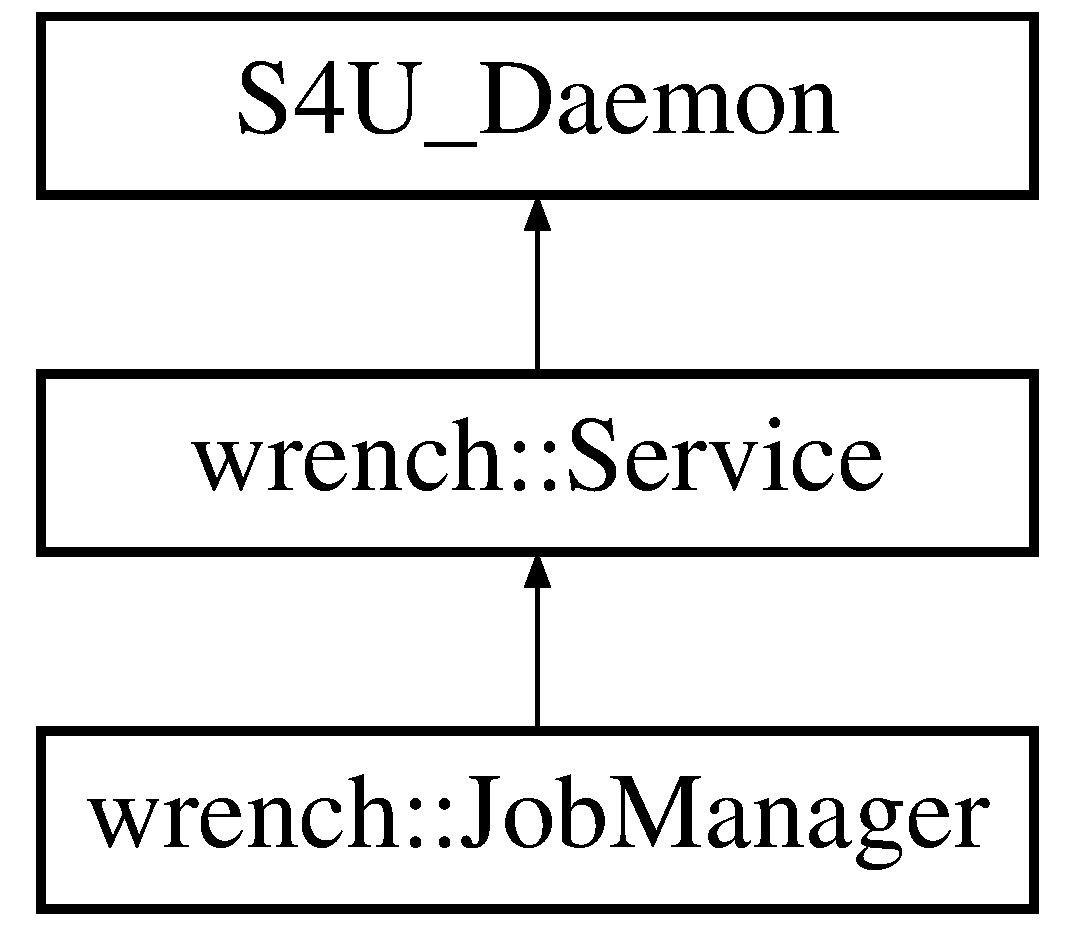
\includegraphics[height=3.000000cm]{classwrench_1_1_job_manager}
\end{center}
\end{figure}
\subsection*{Public Member Functions}
\begin{DoxyCompactItemize}
\item 
\hyperlink{classwrench_1_1_pilot_job}{Pilot\+Job} $\ast$ \hyperlink{classwrench_1_1_job_manager_a9ef786306730359866e3fd2bd3aadaf7}{create\+Pilot\+Job} ()
\begin{DoxyCompactList}\small\item\em Create a pilot job. \end{DoxyCompactList}\item 
\hyperlink{classwrench_1_1_standard_job}{Standard\+Job} $\ast$ \hyperlink{classwrench_1_1_job_manager_a7f3873e56c8813c90b66683690d6b328}{create\+Standard\+Job} (std\+::vector$<$ \hyperlink{classwrench_1_1_workflow_task}{Workflow\+Task} $\ast$$>$ tasks, std\+::map$<$ \hyperlink{classwrench_1_1_workflow_file}{Workflow\+File} $\ast$, \hyperlink{classwrench_1_1_storage_service}{Storage\+Service} $\ast$$>$ file\+\_\+locations, std\+::set$<$ std\+::tuple$<$ \hyperlink{classwrench_1_1_workflow_file}{Workflow\+File} $\ast$, \hyperlink{classwrench_1_1_storage_service}{Storage\+Service} $\ast$, \hyperlink{classwrench_1_1_storage_service}{Storage\+Service} $\ast$$>$$>$ pre\+\_\+file\+\_\+copies, std\+::set$<$ std\+::tuple$<$ \hyperlink{classwrench_1_1_workflow_file}{Workflow\+File} $\ast$, \hyperlink{classwrench_1_1_storage_service}{Storage\+Service} $\ast$, \hyperlink{classwrench_1_1_storage_service}{Storage\+Service} $\ast$$>$$>$ post\+\_\+file\+\_\+copies, std\+::set$<$ std\+::tuple$<$ \hyperlink{classwrench_1_1_workflow_file}{Workflow\+File} $\ast$, \hyperlink{classwrench_1_1_storage_service}{Storage\+Service} $\ast$$>$$>$ cleanup\+\_\+file\+\_\+deletions)
\begin{DoxyCompactList}\small\item\em Create a standard job. \end{DoxyCompactList}\item 
\hyperlink{classwrench_1_1_standard_job}{Standard\+Job} $\ast$ \hyperlink{classwrench_1_1_job_manager_a1dc600a984151ddff2fe5d20525b33bc}{create\+Standard\+Job} (std\+::vector$<$ \hyperlink{classwrench_1_1_workflow_task}{Workflow\+Task} $\ast$$>$ tasks, std\+::map$<$ \hyperlink{classwrench_1_1_workflow_file}{Workflow\+File} $\ast$, \hyperlink{classwrench_1_1_storage_service}{Storage\+Service} $\ast$$>$ file\+\_\+locations)
\begin{DoxyCompactList}\small\item\em Create a standard job. \end{DoxyCompactList}\item 
\hyperlink{classwrench_1_1_standard_job}{Standard\+Job} $\ast$ \hyperlink{classwrench_1_1_job_manager_a42271d359373df86fdb59aeeaf0a4abc}{create\+Standard\+Job} (\hyperlink{classwrench_1_1_workflow_task}{Workflow\+Task} $\ast$task, std\+::map$<$ \hyperlink{classwrench_1_1_workflow_file}{Workflow\+File} $\ast$, \hyperlink{classwrench_1_1_storage_service}{Storage\+Service} $\ast$$>$ file\+\_\+locations)
\begin{DoxyCompactList}\small\item\em Create a standard job. \end{DoxyCompactList}\item 
void \hyperlink{classwrench_1_1_job_manager_ab10f770cc7ce3c022f889ad9cc3fcf0b}{forget\+Job} (\hyperlink{classwrench_1_1_workflow_job}{Workflow\+Job} $\ast$job)
\begin{DoxyCompactList}\small\item\em Forget a job (to free memory, only once a job has completed or failed) \end{DoxyCompactList}\item 
std\+::set$<$ \hyperlink{classwrench_1_1_pilot_job}{Pilot\+Job} $\ast$ $>$ \hyperlink{classwrench_1_1_job_manager_ad7f55858aa45b87289d5f35c4ccfad56}{get\+Pending\+Pilot\+Jobs} ()
\begin{DoxyCompactList}\small\item\em Get the list of currently pending pilot jobs. \end{DoxyCompactList}\item 
std\+::set$<$ \hyperlink{classwrench_1_1_pilot_job}{Pilot\+Job} $\ast$ $>$ \hyperlink{classwrench_1_1_job_manager_aeb91b23edf40378e49929f47e95f1ea6}{get\+Running\+Pilot\+Jobs} ()
\begin{DoxyCompactList}\small\item\em Get the list of currently running pilot jobs. \end{DoxyCompactList}\item 
\mbox{\Hypertarget{classwrench_1_1_job_manager_a7d82fbb044c3fa275f423911b79a7e5c}\label{classwrench_1_1_job_manager_a7d82fbb044c3fa275f423911b79a7e5c}} 
void \hyperlink{classwrench_1_1_job_manager_a7d82fbb044c3fa275f423911b79a7e5c}{kill} ()
\begin{DoxyCompactList}\small\item\em Kill the job manager (brutally terminate the daemon, clears all jobs) \end{DoxyCompactList}\item 
void \hyperlink{classwrench_1_1_job_manager_af9c85f6a54e26f115fa09ef1c9327aa7}{stop} ()
\begin{DoxyCompactList}\small\item\em Stop the job manager. \end{DoxyCompactList}\item 
void \hyperlink{classwrench_1_1_job_manager_a69de09b0d5ae34cbcf9208be88901728}{submit\+Job} (\hyperlink{classwrench_1_1_workflow_job}{Workflow\+Job} $\ast$job, \hyperlink{classwrench_1_1_compute_service}{Compute\+Service} $\ast$compute\+\_\+service, std\+::map$<$ std\+::string, std\+::string $>$ service\+\_\+specific\+\_\+args=\{\})
\begin{DoxyCompactList}\small\item\em Submit a job to compute service. \end{DoxyCompactList}\item 
void \hyperlink{classwrench_1_1_job_manager_aba90476a89bc0748497879bdf07eea9c}{terminate\+Job} (\hyperlink{classwrench_1_1_workflow_job}{Workflow\+Job} $\ast$)
\begin{DoxyCompactList}\small\item\em Terminate a job (standard or pilot) that hasn\textquotesingle{}t completed/expired/failed yet. \end{DoxyCompactList}\end{DoxyCompactItemize}
\subsection*{Additional Inherited Members}


\subsection{Detailed Description}
A helper daemon (co-\/located with and explicitly started by a \hyperlink{classwrench_1_1_w_m_s}{W\+MS}), which is used to handle all job executions. 

\subsection{Member Function Documentation}
\mbox{\Hypertarget{classwrench_1_1_job_manager_a9ef786306730359866e3fd2bd3aadaf7}\label{classwrench_1_1_job_manager_a9ef786306730359866e3fd2bd3aadaf7}} 
\index{wrench\+::\+Job\+Manager@{wrench\+::\+Job\+Manager}!create\+Pilot\+Job@{create\+Pilot\+Job}}
\index{create\+Pilot\+Job@{create\+Pilot\+Job}!wrench\+::\+Job\+Manager@{wrench\+::\+Job\+Manager}}
\subsubsection{\texorpdfstring{create\+Pilot\+Job()}{createPilotJob()}}
{\footnotesize\ttfamily \hyperlink{classwrench_1_1_pilot_job}{Pilot\+Job} $\ast$ wrench\+::\+Job\+Manager\+::create\+Pilot\+Job (\begin{DoxyParamCaption}{ }\end{DoxyParamCaption})}



Create a pilot job. 

\begin{DoxyReturn}{Returns}
the pilot job
\end{DoxyReturn}

\begin{DoxyExceptions}{Exceptions}
{\em std\+::invalid\+\_\+argument} & \\
\hline
\end{DoxyExceptions}
\mbox{\Hypertarget{classwrench_1_1_job_manager_a7f3873e56c8813c90b66683690d6b328}\label{classwrench_1_1_job_manager_a7f3873e56c8813c90b66683690d6b328}} 
\index{wrench\+::\+Job\+Manager@{wrench\+::\+Job\+Manager}!create\+Standard\+Job@{create\+Standard\+Job}}
\index{create\+Standard\+Job@{create\+Standard\+Job}!wrench\+::\+Job\+Manager@{wrench\+::\+Job\+Manager}}
\subsubsection{\texorpdfstring{create\+Standard\+Job()}{createStandardJob()}\hspace{0.1cm}{\footnotesize\ttfamily [1/3]}}
{\footnotesize\ttfamily \hyperlink{classwrench_1_1_standard_job}{Standard\+Job} $\ast$ wrench\+::\+Job\+Manager\+::create\+Standard\+Job (\begin{DoxyParamCaption}\item[{std\+::vector$<$ \hyperlink{classwrench_1_1_workflow_task}{Workflow\+Task} $\ast$$>$}]{tasks,  }\item[{std\+::map$<$ \hyperlink{classwrench_1_1_workflow_file}{Workflow\+File} $\ast$, \hyperlink{classwrench_1_1_storage_service}{Storage\+Service} $\ast$$>$}]{file\+\_\+locations,  }\item[{std\+::set$<$ std\+::tuple$<$ \hyperlink{classwrench_1_1_workflow_file}{Workflow\+File} $\ast$, \hyperlink{classwrench_1_1_storage_service}{Storage\+Service} $\ast$, \hyperlink{classwrench_1_1_storage_service}{Storage\+Service} $\ast$$>$$>$}]{pre\+\_\+file\+\_\+copies,  }\item[{std\+::set$<$ std\+::tuple$<$ \hyperlink{classwrench_1_1_workflow_file}{Workflow\+File} $\ast$, \hyperlink{classwrench_1_1_storage_service}{Storage\+Service} $\ast$, \hyperlink{classwrench_1_1_storage_service}{Storage\+Service} $\ast$$>$$>$}]{post\+\_\+file\+\_\+copies,  }\item[{std\+::set$<$ std\+::tuple$<$ \hyperlink{classwrench_1_1_workflow_file}{Workflow\+File} $\ast$, \hyperlink{classwrench_1_1_storage_service}{Storage\+Service} $\ast$$>$$>$}]{cleanup\+\_\+file\+\_\+deletions }\end{DoxyParamCaption})}



Create a standard job. 


\begin{DoxyParams}{Parameters}
{\em tasks} & a list of tasks (which must be either R\+E\+A\+DY, or children of C\+O\+M\+P\+L\+E\+T\+ED tasks or of tasks also included in the standard job) \\
\hline
{\em file\+\_\+locations} & a map that specifies on which storage services input/output files should be read/written. When unspecified, it is assumed that the \hyperlink{classwrench_1_1_compute_service}{Compute\+Service}\textquotesingle{}s scratch storage space will be used. \\
\hline
{\em pre\+\_\+file\+\_\+copies} & a set of tuples that specify which file copy operations should be completed before task executions begin. The \hyperlink{classwrench_1_1_compute_service_a022e9408f53191b4102e2ce00487799c}{Compute\+Service\+::\+S\+C\+R\+A\+T\+CH} constant can be used to mean \char`\"{}the scratch storage space of the Compute\+Service\char`\"{}. \\
\hline
{\em post\+\_\+file\+\_\+copies} & a set of tuples that specify which file copy operations should be completed after task executions end. The \hyperlink{classwrench_1_1_compute_service_a022e9408f53191b4102e2ce00487799c}{Compute\+Service\+::\+S\+C\+R\+A\+T\+CH} constant can be used to mean \char`\"{}the scratch storage space of the Compute\+Service\char`\"{}. \\
\hline
{\em cleanup\+\_\+file\+\_\+deletions} & a set of file tuples that specify file deletion operations that should be completed at the end of the job. The \hyperlink{classwrench_1_1_compute_service_a022e9408f53191b4102e2ce00487799c}{Compute\+Service\+::\+S\+C\+R\+A\+T\+CH} constant can be used to mean \char`\"{}the scratch storage space of the Compute\+Service\char`\"{}. \\
\hline
\end{DoxyParams}
\begin{DoxyReturn}{Returns}
the standard job
\end{DoxyReturn}

\begin{DoxyExceptions}{Exceptions}
{\em std\+::invalid\+\_\+argument} & \\
\hline
\end{DoxyExceptions}
\mbox{\Hypertarget{classwrench_1_1_job_manager_a1dc600a984151ddff2fe5d20525b33bc}\label{classwrench_1_1_job_manager_a1dc600a984151ddff2fe5d20525b33bc}} 
\index{wrench\+::\+Job\+Manager@{wrench\+::\+Job\+Manager}!create\+Standard\+Job@{create\+Standard\+Job}}
\index{create\+Standard\+Job@{create\+Standard\+Job}!wrench\+::\+Job\+Manager@{wrench\+::\+Job\+Manager}}
\subsubsection{\texorpdfstring{create\+Standard\+Job()}{createStandardJob()}\hspace{0.1cm}{\footnotesize\ttfamily [2/3]}}
{\footnotesize\ttfamily \hyperlink{classwrench_1_1_standard_job}{Standard\+Job} $\ast$ wrench\+::\+Job\+Manager\+::create\+Standard\+Job (\begin{DoxyParamCaption}\item[{std\+::vector$<$ \hyperlink{classwrench_1_1_workflow_task}{Workflow\+Task} $\ast$$>$}]{tasks,  }\item[{std\+::map$<$ \hyperlink{classwrench_1_1_workflow_file}{Workflow\+File} $\ast$, \hyperlink{classwrench_1_1_storage_service}{Storage\+Service} $\ast$$>$}]{file\+\_\+locations }\end{DoxyParamCaption})}



Create a standard job. 


\begin{DoxyParams}{Parameters}
{\em tasks} & a list of tasks (which must be either R\+E\+A\+DY, or children of C\+O\+M\+P\+L\+E\+T\+ED tasks or of tasks also included in the list) \\
\hline
{\em file\+\_\+locations} & a map that specifies on which storage services input/output files should be read/written. When unspecified, it is assumed that the \hyperlink{classwrench_1_1_compute_service}{Compute\+Service}\textquotesingle{}s scratch storage space will be used.\\
\hline
\end{DoxyParams}
\begin{DoxyReturn}{Returns}
the standard job
\end{DoxyReturn}

\begin{DoxyExceptions}{Exceptions}
{\em std\+::invalid\+\_\+argument} & \\
\hline
\end{DoxyExceptions}
\mbox{\Hypertarget{classwrench_1_1_job_manager_a42271d359373df86fdb59aeeaf0a4abc}\label{classwrench_1_1_job_manager_a42271d359373df86fdb59aeeaf0a4abc}} 
\index{wrench\+::\+Job\+Manager@{wrench\+::\+Job\+Manager}!create\+Standard\+Job@{create\+Standard\+Job}}
\index{create\+Standard\+Job@{create\+Standard\+Job}!wrench\+::\+Job\+Manager@{wrench\+::\+Job\+Manager}}
\subsubsection{\texorpdfstring{create\+Standard\+Job()}{createStandardJob()}\hspace{0.1cm}{\footnotesize\ttfamily [3/3]}}
{\footnotesize\ttfamily \hyperlink{classwrench_1_1_standard_job}{Standard\+Job} $\ast$ wrench\+::\+Job\+Manager\+::create\+Standard\+Job (\begin{DoxyParamCaption}\item[{\hyperlink{classwrench_1_1_workflow_task}{Workflow\+Task} $\ast$}]{task,  }\item[{std\+::map$<$ \hyperlink{classwrench_1_1_workflow_file}{Workflow\+File} $\ast$, \hyperlink{classwrench_1_1_storage_service}{Storage\+Service} $\ast$$>$}]{file\+\_\+locations }\end{DoxyParamCaption})}



Create a standard job. 


\begin{DoxyParams}{Parameters}
{\em task} & a task (which must be ready) \\
\hline
{\em file\+\_\+locations} & a map that specifies on which storage services input/output files should be read/written. When unspecified, it is assumed that the \hyperlink{classwrench_1_1_compute_service}{Compute\+Service}\textquotesingle{}s scratch storage space will be used.\\
\hline
\end{DoxyParams}
\begin{DoxyReturn}{Returns}
the standard job
\end{DoxyReturn}

\begin{DoxyExceptions}{Exceptions}
{\em std\+::invalid\+\_\+argument} & \\
\hline
\end{DoxyExceptions}
\mbox{\Hypertarget{classwrench_1_1_job_manager_ab10f770cc7ce3c022f889ad9cc3fcf0b}\label{classwrench_1_1_job_manager_ab10f770cc7ce3c022f889ad9cc3fcf0b}} 
\index{wrench\+::\+Job\+Manager@{wrench\+::\+Job\+Manager}!forget\+Job@{forget\+Job}}
\index{forget\+Job@{forget\+Job}!wrench\+::\+Job\+Manager@{wrench\+::\+Job\+Manager}}
\subsubsection{\texorpdfstring{forget\+Job()}{forgetJob()}}
{\footnotesize\ttfamily void wrench\+::\+Job\+Manager\+::forget\+Job (\begin{DoxyParamCaption}\item[{\hyperlink{classwrench_1_1_workflow_job}{Workflow\+Job} $\ast$}]{job }\end{DoxyParamCaption})}



Forget a job (to free memory, only once a job has completed or failed) 


\begin{DoxyParams}{Parameters}
{\em job} & a job to forget\\
\hline
\end{DoxyParams}

\begin{DoxyExceptions}{Exceptions}
{\em std\+::invalid\+\_\+argument} & \\
\hline
{\em \hyperlink{classwrench_1_1_workflow_execution_exception}{Workflow\+Execution\+Exception}} & \\
\hline
\end{DoxyExceptions}
\mbox{\Hypertarget{classwrench_1_1_job_manager_ad7f55858aa45b87289d5f35c4ccfad56}\label{classwrench_1_1_job_manager_ad7f55858aa45b87289d5f35c4ccfad56}} 
\index{wrench\+::\+Job\+Manager@{wrench\+::\+Job\+Manager}!get\+Pending\+Pilot\+Jobs@{get\+Pending\+Pilot\+Jobs}}
\index{get\+Pending\+Pilot\+Jobs@{get\+Pending\+Pilot\+Jobs}!wrench\+::\+Job\+Manager@{wrench\+::\+Job\+Manager}}
\subsubsection{\texorpdfstring{get\+Pending\+Pilot\+Jobs()}{getPendingPilotJobs()}}
{\footnotesize\ttfamily std\+::set$<$ \hyperlink{classwrench_1_1_pilot_job}{Pilot\+Job} $\ast$ $>$ wrench\+::\+Job\+Manager\+::get\+Pending\+Pilot\+Jobs (\begin{DoxyParamCaption}{ }\end{DoxyParamCaption})}



Get the list of currently pending pilot jobs. 

\begin{DoxyReturn}{Returns}
a set of pilot jobs 
\end{DoxyReturn}
\mbox{\Hypertarget{classwrench_1_1_job_manager_aeb91b23edf40378e49929f47e95f1ea6}\label{classwrench_1_1_job_manager_aeb91b23edf40378e49929f47e95f1ea6}} 
\index{wrench\+::\+Job\+Manager@{wrench\+::\+Job\+Manager}!get\+Running\+Pilot\+Jobs@{get\+Running\+Pilot\+Jobs}}
\index{get\+Running\+Pilot\+Jobs@{get\+Running\+Pilot\+Jobs}!wrench\+::\+Job\+Manager@{wrench\+::\+Job\+Manager}}
\subsubsection{\texorpdfstring{get\+Running\+Pilot\+Jobs()}{getRunningPilotJobs()}}
{\footnotesize\ttfamily std\+::set$<$ \hyperlink{classwrench_1_1_pilot_job}{Pilot\+Job} $\ast$ $>$ wrench\+::\+Job\+Manager\+::get\+Running\+Pilot\+Jobs (\begin{DoxyParamCaption}{ }\end{DoxyParamCaption})}



Get the list of currently running pilot jobs. 

\begin{DoxyReturn}{Returns}
a set of pilot jobs 
\end{DoxyReturn}
\mbox{\Hypertarget{classwrench_1_1_job_manager_af9c85f6a54e26f115fa09ef1c9327aa7}\label{classwrench_1_1_job_manager_af9c85f6a54e26f115fa09ef1c9327aa7}} 
\index{wrench\+::\+Job\+Manager@{wrench\+::\+Job\+Manager}!stop@{stop}}
\index{stop@{stop}!wrench\+::\+Job\+Manager@{wrench\+::\+Job\+Manager}}
\subsubsection{\texorpdfstring{stop()}{stop()}}
{\footnotesize\ttfamily void wrench\+::\+Job\+Manager\+::stop (\begin{DoxyParamCaption}{ }\end{DoxyParamCaption})\hspace{0.3cm}{\ttfamily [virtual]}}



Stop the job manager. 


\begin{DoxyExceptions}{Exceptions}
{\em \hyperlink{classwrench_1_1_workflow_execution_exception}{Workflow\+Execution\+Exception}} & \\
\hline
{\em std\+::runtime\+\_\+error} & \\
\hline
\end{DoxyExceptions}


Reimplemented from \hyperlink{classwrench_1_1_service_ac33a32f4758c6f51b27d2cfb9b46efda}{wrench\+::\+Service}.

\mbox{\Hypertarget{classwrench_1_1_job_manager_a69de09b0d5ae34cbcf9208be88901728}\label{classwrench_1_1_job_manager_a69de09b0d5ae34cbcf9208be88901728}} 
\index{wrench\+::\+Job\+Manager@{wrench\+::\+Job\+Manager}!submit\+Job@{submit\+Job}}
\index{submit\+Job@{submit\+Job}!wrench\+::\+Job\+Manager@{wrench\+::\+Job\+Manager}}
\subsubsection{\texorpdfstring{submit\+Job()}{submitJob()}}
{\footnotesize\ttfamily void wrench\+::\+Job\+Manager\+::submit\+Job (\begin{DoxyParamCaption}\item[{\hyperlink{classwrench_1_1_workflow_job}{Workflow\+Job} $\ast$}]{job,  }\item[{\hyperlink{classwrench_1_1_compute_service}{Compute\+Service} $\ast$}]{compute\+\_\+service,  }\item[{std\+::map$<$ std\+::string, std\+::string $>$}]{service\+\_\+specific\+\_\+args = {\ttfamily \{\}} }\end{DoxyParamCaption})}



Submit a job to compute service. 


\begin{DoxyParams}{Parameters}
{\em job} & a workflow job \\
\hline
{\em compute\+\_\+service} & a compute service \\
\hline
{\em service\+\_\+specific\+\_\+args} & arguments specific for compute services\+:
\begin{DoxyItemize}
\item to a \hyperlink{classwrench_1_1_bare_metal_compute_service}{Bare\+Metal\+Compute\+Service}\+: \{\{\char`\"{}task\+I\+D\char`\"{}, "\mbox{[}hostname\+:\mbox{]}\mbox{[}num\+\_\+cores\mbox{]}\}, ...\}
\begin{DoxyItemize}
\item If no value is not provided for a task, then the service will choose a host and use as many cores as possible on that host.
\item If a \char`\"{}\char`\"{} value is provided for a task, then the service will choose a host and use as many cores as possible on that host.
\item If a \char`\"{}hostname\char`\"{} value is provided for a task, then the service will run the task on that host, using as many of its cores as possible
\item If a \char`\"{}num\+\_\+cores\char`\"{} value is provided for a task, then the service will run that task with this many cores, but will choose the host on which to run it.
\item If a \char`\"{}hostname\+:num\+\_\+cores\char`\"{} value is provided for a task, then the service will run that task with the specified number of cores on that host.
\end{DoxyItemize}
\item to a \hyperlink{classwrench_1_1_batch_service}{Batch\+Service}\+: \{\{\char`\"{}-\/t\char`\"{}\+:\char`\"{}$<$int$>$\char`\"{} (requested number of minutes)\},\{\char`\"{}-\/\+N\char`\"{}\+:\char`\"{}$<$int$>$\char`\"{} (number of requested hosts)\},\{\char`\"{}-\/c\char`\"{}\+:\char`\"{}$<$int$>$\char`\"{} (number of requestes cores per host)\}\}
\item to a \hyperlink{classwrench_1_1_virtualized_cluster_service}{Virtualized\+Cluster\+Service}\+: \{\} (in which case the service will pick the vm) or \{\{\char`\"{}-\/vm\char`\"{}\+:\char`\"{}$<$vm name$>$\char`\"{}\}\}
\item to a \hyperlink{classwrench_1_1_cloud_service}{Cloud\+Service}\+: \{\} (in which case the service will pick the vm) or \{\{\char`\"{}-\/vm\char`\"{}\+:\char`\"{}$<$vm name$>$\char`\"{}\}\}
\end{DoxyItemize}\\
\hline
\end{DoxyParams}

\begin{DoxyExceptions}{Exceptions}
{\em std\+::invalid\+\_\+argument} & \\
\hline
{\em \hyperlink{classwrench_1_1_workflow_execution_exception}{Workflow\+Execution\+Exception}} & \\
\hline
\end{DoxyExceptions}
\mbox{\Hypertarget{classwrench_1_1_job_manager_aba90476a89bc0748497879bdf07eea9c}\label{classwrench_1_1_job_manager_aba90476a89bc0748497879bdf07eea9c}} 
\index{wrench\+::\+Job\+Manager@{wrench\+::\+Job\+Manager}!terminate\+Job@{terminate\+Job}}
\index{terminate\+Job@{terminate\+Job}!wrench\+::\+Job\+Manager@{wrench\+::\+Job\+Manager}}
\subsubsection{\texorpdfstring{terminate\+Job()}{terminateJob()}}
{\footnotesize\ttfamily void wrench\+::\+Job\+Manager\+::terminate\+Job (\begin{DoxyParamCaption}\item[{\hyperlink{classwrench_1_1_workflow_job}{Workflow\+Job} $\ast$}]{job }\end{DoxyParamCaption})}



Terminate a job (standard or pilot) that hasn\textquotesingle{}t completed/expired/failed yet. 


\begin{DoxyParams}{Parameters}
{\em job} & the job to be terminated\\
\hline
\end{DoxyParams}

\begin{DoxyExceptions}{Exceptions}
{\em \hyperlink{classwrench_1_1_workflow_execution_exception}{Workflow\+Execution\+Exception}} & \\
\hline
{\em std\+::invalid\+\_\+argument} & \\
\hline
{\em std\+::runtime\+\_\+error} & \\
\hline
\end{DoxyExceptions}


The documentation for this class was generated from the following files\+:\begin{DoxyCompactItemize}
\item 
/\+Users/rafsilva/\+Documents/isi/workspace/wrench/wrench/include/wrench/managers/Job\+Manager.\+h\item 
/\+Users/rafsilva/\+Documents/isi/workspace/wrench/wrench/src/wrench/managers/Job\+Manager.\+cpp\end{DoxyCompactItemize}

\hypertarget{classwrench_1_1_job_timeout}{}\section{wrench\+:\+:Job\+Timeout Class Reference}
\label{classwrench_1_1_job_timeout}\index{wrench\+::\+Job\+Timeout@{wrench\+::\+Job\+Timeout}}


A \char`\"{}job has times out\char`\"{} failure cause.  




{\ttfamily \#include $<$Failure\+Cause.\+h$>$}

Inheritance diagram for wrench\+:\+:Job\+Timeout\+:\begin{figure}[H]
\begin{center}
\leavevmode
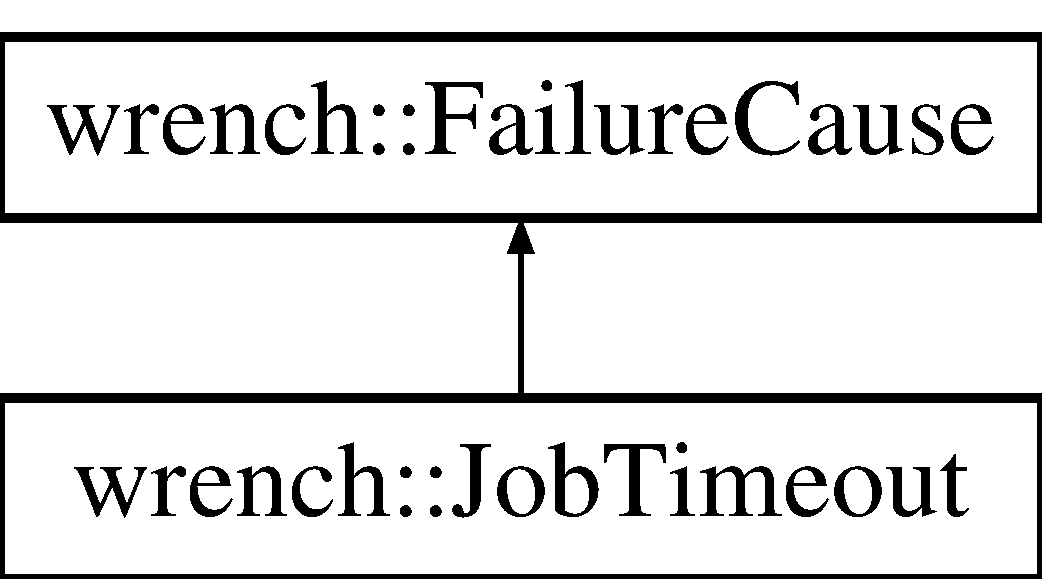
\includegraphics[height=2.000000cm]{classwrench_1_1_job_timeout}
\end{center}
\end{figure}
\subsection*{Public Member Functions}
\begin{DoxyCompactItemize}
\item 
\hyperlink{classwrench_1_1_job_timeout_a352548111a16343238a1376913e80bc6}{Job\+Timeout} (\hyperlink{classwrench_1_1_workflow_job}{Workflow\+Job} $\ast$job)
\begin{DoxyCompactList}\small\item\em Constructor. \end{DoxyCompactList}\item 
\hyperlink{classwrench_1_1_workflow_job}{Workflow\+Job} $\ast$ \hyperlink{classwrench_1_1_job_timeout_a6c3fdde31850803e7eb2e159be735880}{get\+Job} ()
\begin{DoxyCompactList}\small\item\em Getter. \end{DoxyCompactList}\item 
std\+::string \hyperlink{classwrench_1_1_job_timeout_a91515ca59f71777de74a4b0b169d12e7}{to\+String} ()
\begin{DoxyCompactList}\small\item\em Get the human-\/readable failure message. \end{DoxyCompactList}\end{DoxyCompactItemize}
\subsection*{Additional Inherited Members}


\subsection{Detailed Description}
A \char`\"{}job has times out\char`\"{} failure cause. 

\subsection{Constructor \& Destructor Documentation}
\mbox{\Hypertarget{classwrench_1_1_job_timeout_a352548111a16343238a1376913e80bc6}\label{classwrench_1_1_job_timeout_a352548111a16343238a1376913e80bc6}} 
\index{wrench\+::\+Job\+Timeout@{wrench\+::\+Job\+Timeout}!Job\+Timeout@{Job\+Timeout}}
\index{Job\+Timeout@{Job\+Timeout}!wrench\+::\+Job\+Timeout@{wrench\+::\+Job\+Timeout}}
\subsubsection{\texorpdfstring{Job\+Timeout()}{JobTimeout()}}
{\footnotesize\ttfamily wrench\+::\+Job\+Timeout\+::\+Job\+Timeout (\begin{DoxyParamCaption}\item[{\hyperlink{classwrench_1_1_workflow_job}{Workflow\+Job} $\ast$}]{job }\end{DoxyParamCaption})}



Constructor. 


\begin{DoxyParams}{Parameters}
{\em job} & the job that has timed out \\
\hline
\end{DoxyParams}


\subsection{Member Function Documentation}
\mbox{\Hypertarget{classwrench_1_1_job_timeout_a6c3fdde31850803e7eb2e159be735880}\label{classwrench_1_1_job_timeout_a6c3fdde31850803e7eb2e159be735880}} 
\index{wrench\+::\+Job\+Timeout@{wrench\+::\+Job\+Timeout}!get\+Job@{get\+Job}}
\index{get\+Job@{get\+Job}!wrench\+::\+Job\+Timeout@{wrench\+::\+Job\+Timeout}}
\subsubsection{\texorpdfstring{get\+Job()}{getJob()}}
{\footnotesize\ttfamily \hyperlink{classwrench_1_1_workflow_job}{Workflow\+Job} $\ast$ wrench\+::\+Job\+Timeout\+::get\+Job (\begin{DoxyParamCaption}{ }\end{DoxyParamCaption})}



Getter. 

\begin{DoxyReturn}{Returns}
the job 
\end{DoxyReturn}
\mbox{\Hypertarget{classwrench_1_1_job_timeout_a91515ca59f71777de74a4b0b169d12e7}\label{classwrench_1_1_job_timeout_a91515ca59f71777de74a4b0b169d12e7}} 
\index{wrench\+::\+Job\+Timeout@{wrench\+::\+Job\+Timeout}!to\+String@{to\+String}}
\index{to\+String@{to\+String}!wrench\+::\+Job\+Timeout@{wrench\+::\+Job\+Timeout}}
\subsubsection{\texorpdfstring{to\+String()}{toString()}}
{\footnotesize\ttfamily std\+::string wrench\+::\+Job\+Timeout\+::to\+String (\begin{DoxyParamCaption}{ }\end{DoxyParamCaption})\hspace{0.3cm}{\ttfamily [virtual]}}



Get the human-\/readable failure message. 

\begin{DoxyReturn}{Returns}
the message 
\end{DoxyReturn}


Implements \hyperlink{classwrench_1_1_failure_cause_afbad248ebe902409f2cd4f1d6f2b867d}{wrench\+::\+Failure\+Cause}.



The documentation for this class was generated from the following files\+:\begin{DoxyCompactItemize}
\item 
/\+Users/rafsilva/\+Documents/isi/workspace/wrench/wrench/include/wrench/workflow/execution\+\_\+events/Failure\+Cause.\+h\item 
/\+Users/rafsilva/\+Documents/isi/workspace/wrench/wrench/src/wrench/workflow/execution\+\_\+events/Failure\+Cause.\+cpp\end{DoxyCompactItemize}

\hypertarget{classwrench_1_1_job_type_not_supported}{}\section{wrench\+:\+:Job\+Type\+Not\+Supported Class Reference}
\label{classwrench_1_1_job_type_not_supported}\index{wrench\+::\+Job\+Type\+Not\+Supported@{wrench\+::\+Job\+Type\+Not\+Supported}}


A \char`\"{}compute service does not support requested job type\char`\"{} failure cause.  




{\ttfamily \#include $<$Failure\+Cause.\+h$>$}

Inheritance diagram for wrench\+:\+:Job\+Type\+Not\+Supported\+:\begin{figure}[H]
\begin{center}
\leavevmode
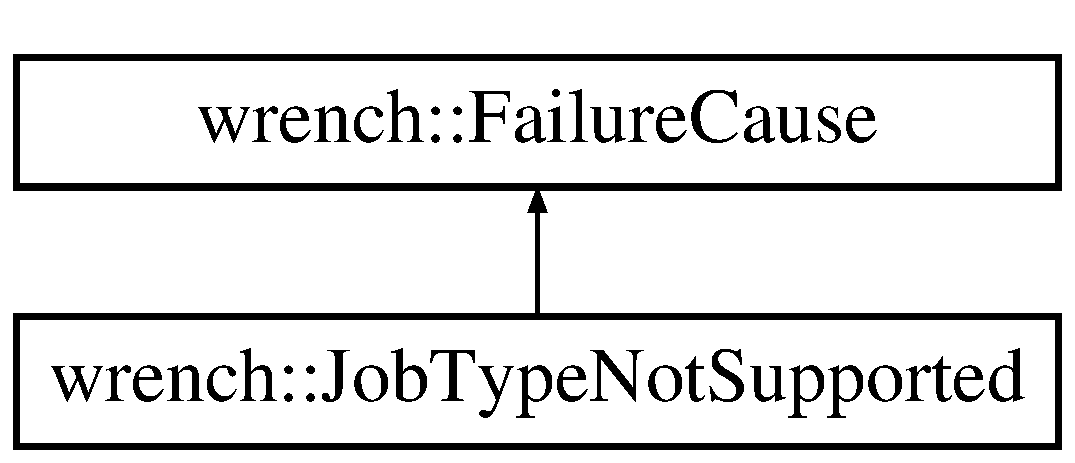
\includegraphics[height=2.000000cm]{classwrench_1_1_job_type_not_supported}
\end{center}
\end{figure}
\subsection*{Public Member Functions}
\begin{DoxyCompactItemize}
\item 
\hyperlink{classwrench_1_1_compute_service}{Compute\+Service} $\ast$ \hyperlink{classwrench_1_1_job_type_not_supported_af2875bcec00418cd655609f1b4f12e55}{get\+Compute\+Service} ()
\begin{DoxyCompactList}\small\item\em Getter. \end{DoxyCompactList}\item 
\hyperlink{classwrench_1_1_workflow_job}{Workflow\+Job} $\ast$ \hyperlink{classwrench_1_1_job_type_not_supported_ade89cf1d1f2a676f5d552b909ef30e5e}{get\+Job} ()
\begin{DoxyCompactList}\small\item\em Getter. \end{DoxyCompactList}\item 
std\+::string \hyperlink{classwrench_1_1_job_type_not_supported_ab6a302367f2db332484da0c256e3ae5c}{to\+String} ()
\begin{DoxyCompactList}\small\item\em Get the human-\/readable failure message. \end{DoxyCompactList}\end{DoxyCompactItemize}
\subsection*{Additional Inherited Members}


\subsection{Detailed Description}
A \char`\"{}compute service does not support requested job type\char`\"{} failure cause. 

\subsection{Member Function Documentation}
\mbox{\Hypertarget{classwrench_1_1_job_type_not_supported_af2875bcec00418cd655609f1b4f12e55}\label{classwrench_1_1_job_type_not_supported_af2875bcec00418cd655609f1b4f12e55}} 
\index{wrench\+::\+Job\+Type\+Not\+Supported@{wrench\+::\+Job\+Type\+Not\+Supported}!get\+Compute\+Service@{get\+Compute\+Service}}
\index{get\+Compute\+Service@{get\+Compute\+Service}!wrench\+::\+Job\+Type\+Not\+Supported@{wrench\+::\+Job\+Type\+Not\+Supported}}
\subsubsection{\texorpdfstring{get\+Compute\+Service()}{getComputeService()}}
{\footnotesize\ttfamily \hyperlink{classwrench_1_1_compute_service}{Compute\+Service} $\ast$ wrench\+::\+Job\+Type\+Not\+Supported\+::get\+Compute\+Service (\begin{DoxyParamCaption}{ }\end{DoxyParamCaption})}



Getter. 

\begin{DoxyReturn}{Returns}
the compute service 
\end{DoxyReturn}
\mbox{\Hypertarget{classwrench_1_1_job_type_not_supported_ade89cf1d1f2a676f5d552b909ef30e5e}\label{classwrench_1_1_job_type_not_supported_ade89cf1d1f2a676f5d552b909ef30e5e}} 
\index{wrench\+::\+Job\+Type\+Not\+Supported@{wrench\+::\+Job\+Type\+Not\+Supported}!get\+Job@{get\+Job}}
\index{get\+Job@{get\+Job}!wrench\+::\+Job\+Type\+Not\+Supported@{wrench\+::\+Job\+Type\+Not\+Supported}}
\subsubsection{\texorpdfstring{get\+Job()}{getJob()}}
{\footnotesize\ttfamily \hyperlink{classwrench_1_1_workflow_job}{Workflow\+Job} $\ast$ wrench\+::\+Job\+Type\+Not\+Supported\+::get\+Job (\begin{DoxyParamCaption}{ }\end{DoxyParamCaption})}



Getter. 

\begin{DoxyReturn}{Returns}
the job 
\end{DoxyReturn}
\mbox{\Hypertarget{classwrench_1_1_job_type_not_supported_ab6a302367f2db332484da0c256e3ae5c}\label{classwrench_1_1_job_type_not_supported_ab6a302367f2db332484da0c256e3ae5c}} 
\index{wrench\+::\+Job\+Type\+Not\+Supported@{wrench\+::\+Job\+Type\+Not\+Supported}!to\+String@{to\+String}}
\index{to\+String@{to\+String}!wrench\+::\+Job\+Type\+Not\+Supported@{wrench\+::\+Job\+Type\+Not\+Supported}}
\subsubsection{\texorpdfstring{to\+String()}{toString()}}
{\footnotesize\ttfamily std\+::string wrench\+::\+Job\+Type\+Not\+Supported\+::to\+String (\begin{DoxyParamCaption}{ }\end{DoxyParamCaption})\hspace{0.3cm}{\ttfamily [virtual]}}



Get the human-\/readable failure message. 

\begin{DoxyReturn}{Returns}
the message 
\end{DoxyReturn}


Implements \hyperlink{classwrench_1_1_failure_cause_afbad248ebe902409f2cd4f1d6f2b867d}{wrench\+::\+Failure\+Cause}.



The documentation for this class was generated from the following files\+:\begin{DoxyCompactItemize}
\item 
/\+Users/rafsilva/\+Documents/isi/workspace/wrench/wrench/include/wrench/workflow/execution\+\_\+events/Failure\+Cause.\+h\item 
/\+Users/rafsilva/\+Documents/isi/workspace/wrench/wrench/src/wrench/workflow/execution\+\_\+events/Failure\+Cause.\+cpp\end{DoxyCompactItemize}

\hypertarget{classwrench_1_1_negotiator_completion_message}{}\section{wrench\+:\+:Negotiator\+Completion\+Message Class Reference}
\label{classwrench_1_1_negotiator_completion_message}\index{wrench\+::\+Negotiator\+Completion\+Message@{wrench\+::\+Negotiator\+Completion\+Message}}
Inheritance diagram for wrench\+:\+:Negotiator\+Completion\+Message\+:\begin{figure}[H]
\begin{center}
\leavevmode
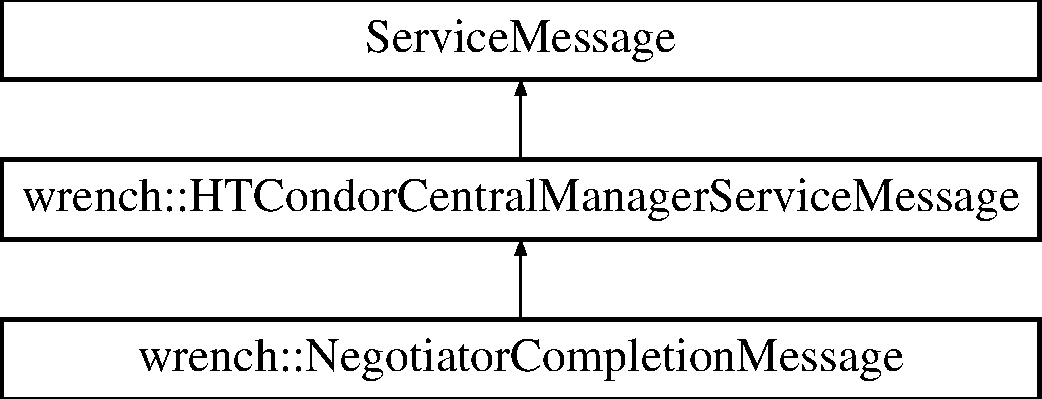
\includegraphics[height=3.000000cm]{classwrench_1_1_negotiator_completion_message}
\end{center}
\end{figure}
\subsection*{Public Member Functions}
\begin{DoxyCompactItemize}
\item 
\hyperlink{classwrench_1_1_negotiator_completion_message_aece506a0df6a8a5bf7484467f05c9b19}{Negotiator\+Completion\+Message} (std\+::vector$<$ Standard\+Job $\ast$$>$ scheduled\+\_\+jobs, double payload)
\begin{DoxyCompactList}\small\item\em Constructor. \end{DoxyCompactList}\end{DoxyCompactItemize}
\subsection*{Public Attributes}
\begin{DoxyCompactItemize}
\item 
\mbox{\Hypertarget{classwrench_1_1_negotiator_completion_message_aeaf67aaa5ac0bc830eff59ef6d51d9d5}\label{classwrench_1_1_negotiator_completion_message_aeaf67aaa5ac0bc830eff59ef6d51d9d5}} 
std\+::vector$<$ Standard\+Job $\ast$ $>$ {\bfseries scheduled\+\_\+jobs}
\end{DoxyCompactItemize}
\subsection*{Additional Inherited Members}


\subsection{Constructor \& Destructor Documentation}
\mbox{\Hypertarget{classwrench_1_1_negotiator_completion_message_aece506a0df6a8a5bf7484467f05c9b19}\label{classwrench_1_1_negotiator_completion_message_aece506a0df6a8a5bf7484467f05c9b19}} 
\index{wrench\+::\+Negotiator\+Completion\+Message@{wrench\+::\+Negotiator\+Completion\+Message}!Negotiator\+Completion\+Message@{Negotiator\+Completion\+Message}}
\index{Negotiator\+Completion\+Message@{Negotiator\+Completion\+Message}!wrench\+::\+Negotiator\+Completion\+Message@{wrench\+::\+Negotiator\+Completion\+Message}}
\subsubsection{\texorpdfstring{Negotiator\+Completion\+Message()}{NegotiatorCompletionMessage()}}
{\footnotesize\ttfamily wrench\+::\+Negotiator\+Completion\+Message\+::\+Negotiator\+Completion\+Message (\begin{DoxyParamCaption}\item[{std\+::vector$<$ Standard\+Job $\ast$$>$}]{scheduled\+\_\+jobs,  }\item[{double}]{payload }\end{DoxyParamCaption})}



Constructor. 


\begin{DoxyParams}{Parameters}
{\em scheduled\+\_\+jobs} & list of pending jobs upon negotiator completion \\
\hline
{\em payload} & the message size in bytes \\
\hline
\end{DoxyParams}


The documentation for this class was generated from the following files\+:\begin{DoxyCompactItemize}
\item 
/\+Users/rafsilva/\+Documents/isi/workspace/wrench/wrench/include/wrench/services/compute/htcondor/H\+T\+Condor\+Central\+Manager\+Service\+Message.\+h\item 
/\+Users/rafsilva/\+Documents/isi/workspace/wrench/wrench/src/wrench/services/compute/htcondor/H\+T\+Condor\+Central\+Manager\+Service\+Message.\+cpp\end{DoxyCompactItemize}

\hypertarget{classwrench_1_1_network_error}{}\section{wrench\+:\+:Network\+Error Class Reference}
\label{classwrench_1_1_network_error}\index{wrench\+::\+Network\+Error@{wrench\+::\+Network\+Error}}


A \char`\"{}network error (or endpoint is down)\char`\"{} failure cause.  




{\ttfamily \#include $<$Failure\+Cause.\+h$>$}

Inheritance diagram for wrench\+:\+:Network\+Error\+:\begin{figure}[H]
\begin{center}
\leavevmode
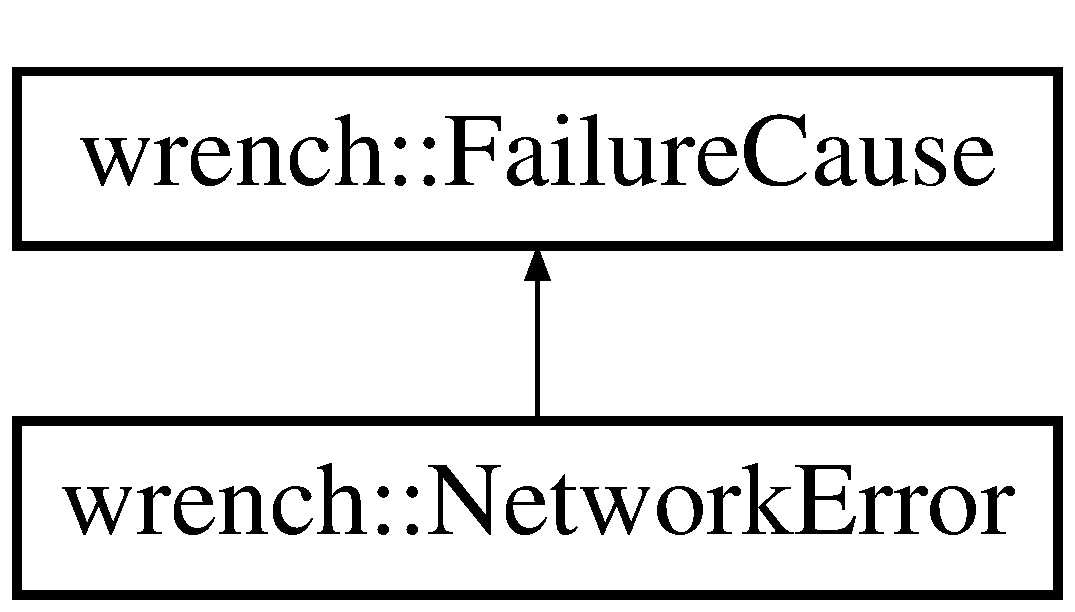
\includegraphics[height=2.000000cm]{classwrench_1_1_network_error}
\end{center}
\end{figure}
\subsection*{Public Types}
\begin{DoxyCompactItemize}
\item 
\mbox{\Hypertarget{classwrench_1_1_network_error_a17ec7046bb91ea4e909c3bf59d46f09b}\label{classwrench_1_1_network_error_a17ec7046bb91ea4e909c3bf59d46f09b}} 
enum \hyperlink{classwrench_1_1_network_error_a17ec7046bb91ea4e909c3bf59d46f09b}{Error\+Type} \{ {\bfseries T\+I\+M\+E\+O\+UT}, 
{\bfseries F\+A\+I\+L\+U\+RE}
 \}\begin{DoxyCompactList}\small\item\em Enumerated type to describe the type of the network error. \end{DoxyCompactList}
\item 
\mbox{\Hypertarget{classwrench_1_1_network_error_a18331f823c565c53be139bdac90437d8}\label{classwrench_1_1_network_error_a18331f823c565c53be139bdac90437d8}} 
enum \hyperlink{classwrench_1_1_network_error_a18331f823c565c53be139bdac90437d8}{Operation\+Type} \{ {\bfseries S\+E\+N\+D\+I\+NG}, 
{\bfseries R\+E\+C\+E\+I\+V\+I\+NG}
 \}\begin{DoxyCompactList}\small\item\em Enumerated type to describe whether the network error occured while sending or receiving. \end{DoxyCompactList}
\end{DoxyCompactItemize}
\subsection*{Public Member Functions}
\begin{DoxyCompactItemize}
\item 
\hyperlink{classwrench_1_1_network_error_ac7718f7a5172d75aeee99b320ddc5487}{Network\+Error} (\hyperlink{classwrench_1_1_network_error_a18331f823c565c53be139bdac90437d8}{Network\+Error\+::\+Operation\+Type}, \hyperlink{classwrench_1_1_network_error_a17ec7046bb91ea4e909c3bf59d46f09b}{Network\+Error\+::\+Error\+Type}, std\+::string mailbox)
\begin{DoxyCompactList}\small\item\em Constructor. \end{DoxyCompactList}\item 
std\+::string \hyperlink{classwrench_1_1_network_error_a0760db02c40d2ba195aa87106951411f}{get\+Mailbox} ()
\begin{DoxyCompactList}\small\item\em Returns the mailbox name on which the error occurred. \end{DoxyCompactList}\item 
bool \hyperlink{classwrench_1_1_network_error_a4aed0a6b6496e19e70e16da31eae8b19}{is\+Timeout} ()
\begin{DoxyCompactList}\small\item\em Returns whether the network error was a timeout. \end{DoxyCompactList}\item 
std\+::string \hyperlink{classwrench_1_1_network_error_a114346c3faa84b3925600e9a22314a37}{to\+String} ()
\begin{DoxyCompactList}\small\item\em Get the human-\/readable failure message. \end{DoxyCompactList}\item 
bool \hyperlink{classwrench_1_1_network_error_a1fa6782fde91dab538f577d2608eb640}{while\+Receiving} ()
\begin{DoxyCompactList}\small\item\em Returns whether the network error occurred while receiving. \end{DoxyCompactList}\item 
bool \hyperlink{classwrench_1_1_network_error_a98a2da5f34bd18fc2c245b364e884b34}{while\+Sending} ()
\begin{DoxyCompactList}\small\item\em Returns whether the network error occurred while sending. \end{DoxyCompactList}\end{DoxyCompactItemize}


\subsection{Detailed Description}
A \char`\"{}network error (or endpoint is down)\char`\"{} failure cause. 

\subsection{Constructor \& Destructor Documentation}
\mbox{\Hypertarget{classwrench_1_1_network_error_ac7718f7a5172d75aeee99b320ddc5487}\label{classwrench_1_1_network_error_ac7718f7a5172d75aeee99b320ddc5487}} 
\index{wrench\+::\+Network\+Error@{wrench\+::\+Network\+Error}!Network\+Error@{Network\+Error}}
\index{Network\+Error@{Network\+Error}!wrench\+::\+Network\+Error@{wrench\+::\+Network\+Error}}
\subsubsection{\texorpdfstring{Network\+Error()}{NetworkError()}}
{\footnotesize\ttfamily wrench\+::\+Network\+Error\+::\+Network\+Error (\begin{DoxyParamCaption}\item[{\hyperlink{classwrench_1_1_network_error_a18331f823c565c53be139bdac90437d8}{Network\+Error\+::\+Operation\+Type}}]{operation\+\_\+type,  }\item[{\hyperlink{classwrench_1_1_network_error_a17ec7046bb91ea4e909c3bf59d46f09b}{Network\+Error\+::\+Error\+Type}}]{error\+\_\+type,  }\item[{std\+::string}]{mailbox }\end{DoxyParamCaption})}



Constructor. 


\begin{DoxyParams}{Parameters}
{\em operation\+\_\+type} & Network\+Error\+:\+Operation\+Type\+:\+:S\+E\+N\+D\+I\+NG or Network\+Error\+::\+Operation\+Type\+::\+R\+E\+C\+E\+I\+V\+I\+NG \\
\hline
{\em mailbox} & the name of a mailbox \\
\hline
\end{DoxyParams}


\subsection{Member Function Documentation}
\mbox{\Hypertarget{classwrench_1_1_network_error_a0760db02c40d2ba195aa87106951411f}\label{classwrench_1_1_network_error_a0760db02c40d2ba195aa87106951411f}} 
\index{wrench\+::\+Network\+Error@{wrench\+::\+Network\+Error}!get\+Mailbox@{get\+Mailbox}}
\index{get\+Mailbox@{get\+Mailbox}!wrench\+::\+Network\+Error@{wrench\+::\+Network\+Error}}
\subsubsection{\texorpdfstring{get\+Mailbox()}{getMailbox()}}
{\footnotesize\ttfamily std\+::string wrench\+::\+Network\+Error\+::get\+Mailbox (\begin{DoxyParamCaption}{ }\end{DoxyParamCaption})}



Returns the mailbox name on which the error occurred. 

\begin{DoxyReturn}{Returns}
the mailbox name 
\end{DoxyReturn}
\mbox{\Hypertarget{classwrench_1_1_network_error_a4aed0a6b6496e19e70e16da31eae8b19}\label{classwrench_1_1_network_error_a4aed0a6b6496e19e70e16da31eae8b19}} 
\index{wrench\+::\+Network\+Error@{wrench\+::\+Network\+Error}!is\+Timeout@{is\+Timeout}}
\index{is\+Timeout@{is\+Timeout}!wrench\+::\+Network\+Error@{wrench\+::\+Network\+Error}}
\subsubsection{\texorpdfstring{is\+Timeout()}{isTimeout()}}
{\footnotesize\ttfamily bool wrench\+::\+Network\+Error\+::is\+Timeout (\begin{DoxyParamCaption}{ }\end{DoxyParamCaption})}



Returns whether the network error was a timeout. 

\begin{DoxyReturn}{Returns}
true or false 
\end{DoxyReturn}
\mbox{\Hypertarget{classwrench_1_1_network_error_a114346c3faa84b3925600e9a22314a37}\label{classwrench_1_1_network_error_a114346c3faa84b3925600e9a22314a37}} 
\index{wrench\+::\+Network\+Error@{wrench\+::\+Network\+Error}!to\+String@{to\+String}}
\index{to\+String@{to\+String}!wrench\+::\+Network\+Error@{wrench\+::\+Network\+Error}}
\subsubsection{\texorpdfstring{to\+String()}{toString()}}
{\footnotesize\ttfamily std\+::string wrench\+::\+Network\+Error\+::to\+String (\begin{DoxyParamCaption}{ }\end{DoxyParamCaption})\hspace{0.3cm}{\ttfamily [virtual]}}



Get the human-\/readable failure message. 

\begin{DoxyReturn}{Returns}
the message 
\end{DoxyReturn}


Implements \hyperlink{classwrench_1_1_failure_cause_afbad248ebe902409f2cd4f1d6f2b867d}{wrench\+::\+Failure\+Cause}.

\mbox{\Hypertarget{classwrench_1_1_network_error_a1fa6782fde91dab538f577d2608eb640}\label{classwrench_1_1_network_error_a1fa6782fde91dab538f577d2608eb640}} 
\index{wrench\+::\+Network\+Error@{wrench\+::\+Network\+Error}!while\+Receiving@{while\+Receiving}}
\index{while\+Receiving@{while\+Receiving}!wrench\+::\+Network\+Error@{wrench\+::\+Network\+Error}}
\subsubsection{\texorpdfstring{while\+Receiving()}{whileReceiving()}}
{\footnotesize\ttfamily bool wrench\+::\+Network\+Error\+::while\+Receiving (\begin{DoxyParamCaption}{ }\end{DoxyParamCaption})}



Returns whether the network error occurred while receiving. 

\begin{DoxyReturn}{Returns}
true or false 
\end{DoxyReturn}
\mbox{\Hypertarget{classwrench_1_1_network_error_a98a2da5f34bd18fc2c245b364e884b34}\label{classwrench_1_1_network_error_a98a2da5f34bd18fc2c245b364e884b34}} 
\index{wrench\+::\+Network\+Error@{wrench\+::\+Network\+Error}!while\+Sending@{while\+Sending}}
\index{while\+Sending@{while\+Sending}!wrench\+::\+Network\+Error@{wrench\+::\+Network\+Error}}
\subsubsection{\texorpdfstring{while\+Sending()}{whileSending()}}
{\footnotesize\ttfamily bool wrench\+::\+Network\+Error\+::while\+Sending (\begin{DoxyParamCaption}{ }\end{DoxyParamCaption})}



Returns whether the network error occurred while sending. 

\begin{DoxyReturn}{Returns}
true or false 
\end{DoxyReturn}


The documentation for this class was generated from the following files\+:\begin{DoxyCompactItemize}
\item 
/\+Users/rafsilva/\+Documents/isi/workspace/wrench/wrench/include/wrench/workflow/execution\+\_\+events/Failure\+Cause.\+h\item 
/\+Users/rafsilva/\+Documents/isi/workspace/wrench/wrench/src/wrench/workflow/execution\+\_\+events/Failure\+Cause.\+cpp\end{DoxyCompactItemize}

\hypertarget{classwrench_1_1_network_proximity_service}{}\section{wrench\+:\+:Network\+Proximity\+Service Class Reference}
\label{classwrench_1_1_network_proximity_service}\index{wrench\+::\+Network\+Proximity\+Service@{wrench\+::\+Network\+Proximity\+Service}}


A network proximity service that continuously estimates inter-\/host latencies and can be queried for such estimates.  




{\ttfamily \#include $<$Network\+Proximity\+Service.\+h$>$}

Inheritance diagram for wrench\+:\+:Network\+Proximity\+Service\+:\begin{figure}[H]
\begin{center}
\leavevmode
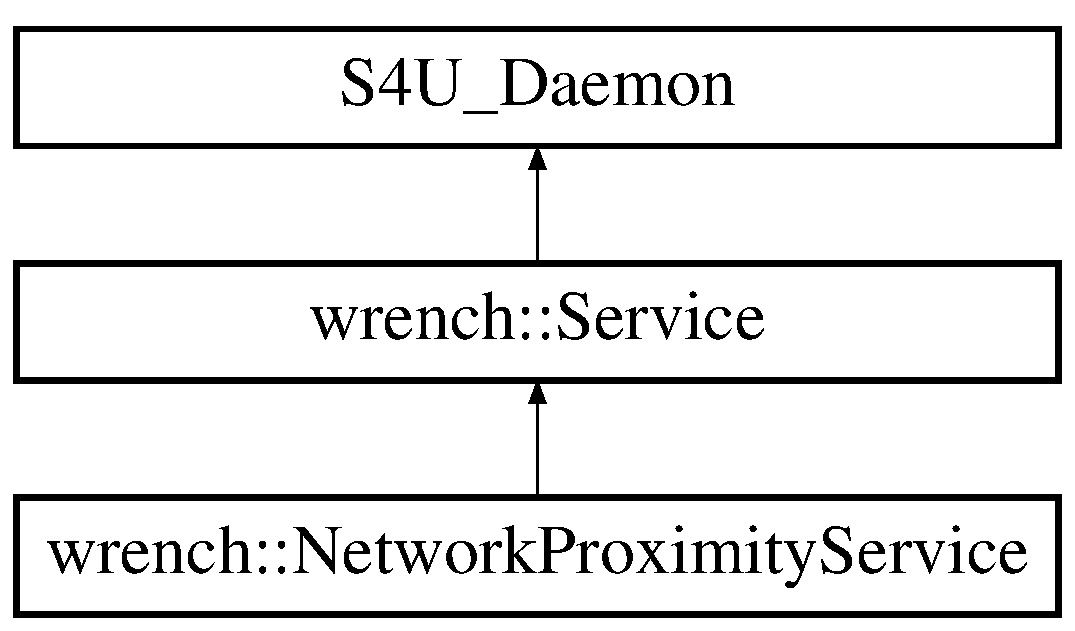
\includegraphics[height=3.000000cm]{classwrench_1_1_network_proximity_service}
\end{center}
\end{figure}
\subsection*{Public Member Functions}
\begin{DoxyCompactItemize}
\item 
\hyperlink{classwrench_1_1_network_proximity_service_a8f7021f0fd9a5a6393fc447652c2371b}{Network\+Proximity\+Service} (std\+::string db\+\_\+hostname, std\+::vector$<$ std\+::string $>$ hosts\+\_\+in\+\_\+network, std\+::map$<$ std\+::string, std\+::string $>$=\{\}, std\+::map$<$ std\+::string, std\+::string $>$=\{\})
\begin{DoxyCompactList}\small\item\em Constructor. \end{DoxyCompactList}\end{DoxyCompactItemize}


\subsection{Detailed Description}
A network proximity service that continuously estimates inter-\/host latencies and can be queried for such estimates. 

\subsection{Constructor \& Destructor Documentation}
\mbox{\Hypertarget{classwrench_1_1_network_proximity_service_a8f7021f0fd9a5a6393fc447652c2371b}\label{classwrench_1_1_network_proximity_service_a8f7021f0fd9a5a6393fc447652c2371b}} 
\index{wrench\+::\+Network\+Proximity\+Service@{wrench\+::\+Network\+Proximity\+Service}!Network\+Proximity\+Service@{Network\+Proximity\+Service}}
\index{Network\+Proximity\+Service@{Network\+Proximity\+Service}!wrench\+::\+Network\+Proximity\+Service@{wrench\+::\+Network\+Proximity\+Service}}
\subsubsection{\texorpdfstring{Network\+Proximity\+Service()}{NetworkProximityService()}}
{\footnotesize\ttfamily wrench\+::\+Network\+Proximity\+Service\+::\+Network\+Proximity\+Service (\begin{DoxyParamCaption}\item[{std\+::string}]{hostname,  }\item[{std\+::vector$<$ std\+::string $>$}]{hosts\+\_\+in\+\_\+network,  }\item[{std\+::map$<$ std\+::string, std\+::string $>$}]{property\+\_\+list = {\ttfamily \{\}},  }\item[{std\+::map$<$ std\+::string, std\+::string $>$}]{messagepayload\+\_\+list = {\ttfamily \{\}} }\end{DoxyParamCaption})}



Constructor. 


\begin{DoxyParams}{Parameters}
{\em hostname} & the name of the host on which to start the service \\
\hline
{\em hosts\+\_\+in\+\_\+network} & the hosts participating in network measurements \\
\hline
{\em property\+\_\+list} & a property list (\{\} means \char`\"{}use all defaults\char`\"{}) \\
\hline
{\em messagepayload\+\_\+list} & a message payload list (\{\} means \char`\"{}use all defaults\char`\"{}) \\
\hline
\end{DoxyParams}


The documentation for this class was generated from the following files\+:\begin{DoxyCompactItemize}
\item 
/\+Users/rafsilva/\+Documents/isi/workspace/wrench/wrench/include/wrench/services/network\+\_\+proximity/Network\+Proximity\+Service.\+h\item 
/\+Users/rafsilva/\+Documents/isi/workspace/wrench/wrench/src/wrench/services/network\+\_\+proximity/Network\+Proximity\+Service.\+cpp\end{DoxyCompactItemize}

\hypertarget{classwrench_1_1_network_proximity_service_message_payload}{}\section{wrench\+:\+:Network\+Proximity\+Service\+Message\+Payload Class Reference}
\label{classwrench_1_1_network_proximity_service_message_payload}\index{wrench\+::\+Network\+Proximity\+Service\+Message\+Payload@{wrench\+::\+Network\+Proximity\+Service\+Message\+Payload}}


Configurable message payloads for a \hyperlink{classwrench_1_1_network_proximity_service}{Network\+Proximity\+Service}.  




{\ttfamily \#include $<$Network\+Proximity\+Service\+Message\+Payload.\+h$>$}

Inheritance diagram for wrench\+:\+:Network\+Proximity\+Service\+Message\+Payload\+:\begin{figure}[H]
\begin{center}
\leavevmode
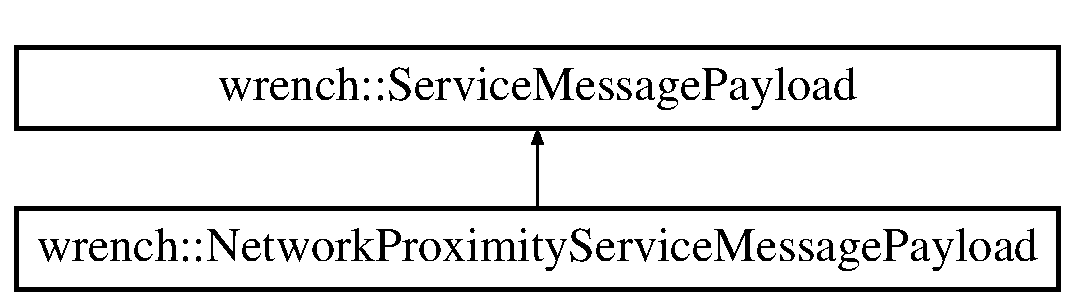
\includegraphics[height=2.000000cm]{classwrench_1_1_network_proximity_service_message_payload}
\end{center}
\end{figure}
\subsection*{Static Public Attributes}
\begin{DoxyCompactItemize}
\item 
\mbox{\Hypertarget{classwrench_1_1_network_proximity_service_message_payload_ad265658bc0467be580921500ba87e4ae}\label{classwrench_1_1_network_proximity_service_message_payload_ad265658bc0467be580921500ba87e4ae}} 
static const std\+::string \hyperlink{classwrench_1_1_network_proximity_service_message_payload_ad265658bc0467be580921500ba87e4ae}{N\+E\+T\+W\+O\+R\+K\+\_\+\+D\+A\+E\+M\+O\+N\+\_\+\+C\+O\+N\+T\+A\+C\+T\+\_\+\+A\+N\+S\+W\+E\+R\+\_\+\+P\+A\+Y\+L\+O\+AD}
\begin{DoxyCompactList}\small\item\em The number of bytes in the message sent by the service to a network proximity daemon in answer to a request for which other network proximity daemon to run network proximity experiments with. \end{DoxyCompactList}\item 
\mbox{\Hypertarget{classwrench_1_1_network_proximity_service_message_payload_aea4a6c68427d8867a296712dd932de76}\label{classwrench_1_1_network_proximity_service_message_payload_aea4a6c68427d8867a296712dd932de76}} 
static const std\+::string \hyperlink{classwrench_1_1_network_proximity_service_message_payload_aea4a6c68427d8867a296712dd932de76}{N\+E\+T\+W\+O\+R\+K\+\_\+\+D\+A\+E\+M\+O\+N\+\_\+\+C\+O\+N\+T\+A\+C\+T\+\_\+\+R\+E\+Q\+U\+E\+S\+T\+\_\+\+P\+A\+Y\+L\+O\+AD}
\begin{DoxyCompactList}\small\item\em The number of bytes in the message sent by a network proximity daemon to the network proximity service to request which other network proximity daemon it should run network proximity experiments with. \end{DoxyCompactList}\item 
\mbox{\Hypertarget{classwrench_1_1_network_proximity_service_message_payload_ab1c52bc80c038950b69e861a3fba75a6}\label{classwrench_1_1_network_proximity_service_message_payload_ab1c52bc80c038950b69e861a3fba75a6}} 
static const std\+::string \hyperlink{classwrench_1_1_network_proximity_service_message_payload_ab1c52bc80c038950b69e861a3fba75a6}{N\+E\+T\+W\+O\+R\+K\+\_\+\+D\+A\+E\+M\+O\+N\+\_\+\+M\+E\+A\+S\+U\+R\+E\+M\+E\+N\+T\+\_\+\+R\+E\+P\+O\+R\+T\+I\+N\+G\+\_\+\+P\+A\+Y\+L\+O\+AD}
\begin{DoxyCompactList}\small\item\em The number of bytes in the message sent by a network proximity daemon to the network proximity service to report on an R\+TT measurement experiment. \end{DoxyCompactList}\item 
\mbox{\Hypertarget{classwrench_1_1_network_proximity_service_message_payload_ae8db9b59fd8a8ba3b3acb54c4b59f31a}\label{classwrench_1_1_network_proximity_service_message_payload_ae8db9b59fd8a8ba3b3acb54c4b59f31a}} 
static const std\+::string \hyperlink{classwrench_1_1_network_proximity_service_message_payload_ae8db9b59fd8a8ba3b3acb54c4b59f31a}{N\+E\+T\+W\+O\+R\+K\+\_\+\+D\+B\+\_\+\+L\+O\+O\+K\+U\+P\+\_\+\+A\+N\+S\+W\+E\+R\+\_\+\+M\+E\+S\+S\+A\+G\+E\+\_\+\+P\+A\+Y\+L\+O\+AD}
\begin{DoxyCompactList}\small\item\em The number of bytes in the message sent by the service in answer to a request for a proximity value lookup. \end{DoxyCompactList}\item 
\mbox{\Hypertarget{classwrench_1_1_network_proximity_service_message_payload_a495eafbd2b9f58a992d20ed10bc714d4}\label{classwrench_1_1_network_proximity_service_message_payload_a495eafbd2b9f58a992d20ed10bc714d4}} 
static const std\+::string \hyperlink{classwrench_1_1_network_proximity_service_message_payload_a495eafbd2b9f58a992d20ed10bc714d4}{N\+E\+T\+W\+O\+R\+K\+\_\+\+D\+B\+\_\+\+L\+O\+O\+K\+U\+P\+\_\+\+R\+E\+Q\+U\+E\+S\+T\+\_\+\+M\+E\+S\+S\+A\+G\+E\+\_\+\+P\+A\+Y\+L\+O\+AD}
\begin{DoxyCompactList}\small\item\em The number of bytes in the message sent to the service to request a proximity value lookup. \end{DoxyCompactList}\end{DoxyCompactItemize}


\subsection{Detailed Description}
Configurable message payloads for a \hyperlink{classwrench_1_1_network_proximity_service}{Network\+Proximity\+Service}. 

The documentation for this class was generated from the following file\+:\begin{DoxyCompactItemize}
\item 
/\+Users/rafsilva/\+Documents/isi/workspace/wrench/wrench/include/wrench/services/network\+\_\+proximity/Network\+Proximity\+Service\+Message\+Payload.\+h\end{DoxyCompactItemize}

\hypertarget{classwrench_1_1_network_proximity_service_property}{}\section{wrench\+:\+:Network\+Proximity\+Service\+Property Class Reference}
\label{classwrench_1_1_network_proximity_service_property}\index{wrench\+::\+Network\+Proximity\+Service\+Property@{wrench\+::\+Network\+Proximity\+Service\+Property}}


Configurable properties for a \hyperlink{classwrench_1_1_network_proximity_service}{Network\+Proximity\+Service}.  




{\ttfamily \#include $<$Network\+Proximity\+Service\+Property.\+h$>$}

Inheritance diagram for wrench\+:\+:Network\+Proximity\+Service\+Property\+:\begin{figure}[H]
\begin{center}
\leavevmode
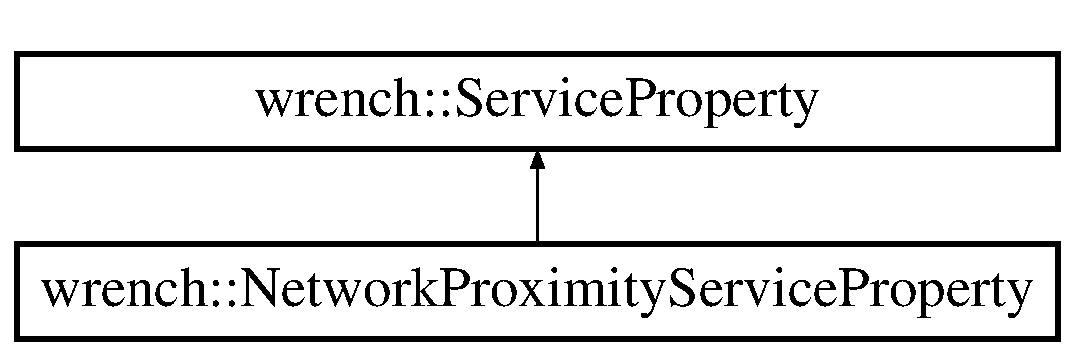
\includegraphics[height=2.000000cm]{classwrench_1_1_network_proximity_service_property}
\end{center}
\end{figure}
\subsection*{Static Public Attributes}
\begin{DoxyCompactItemize}
\item 
\mbox{\Hypertarget{classwrench_1_1_network_proximity_service_property_a180718956b9f9b7bf040cc60dcef65f7}\label{classwrench_1_1_network_proximity_service_property_a180718956b9f9b7bf040cc60dcef65f7}} 
static const std\+::string \hyperlink{classwrench_1_1_network_proximity_service_property_a180718956b9f9b7bf040cc60dcef65f7}{L\+O\+O\+K\+U\+P\+\_\+\+O\+V\+E\+R\+H\+E\+AD}
\begin{DoxyCompactList}\small\item\em The overhead, in seconds, of looking up entries for a file (default\+: 0) \end{DoxyCompactList}\item 
\mbox{\Hypertarget{classwrench_1_1_network_proximity_service_property_a19af22a3ba877db9832cd764de95d3d8}\label{classwrench_1_1_network_proximity_service_property_a19af22a3ba877db9832cd764de95d3d8}} 
static const std\+::string \hyperlink{classwrench_1_1_network_proximity_service_property_a19af22a3ba877db9832cd764de95d3d8}{N\+E\+T\+W\+O\+R\+K\+\_\+\+D\+A\+E\+M\+O\+N\+\_\+\+C\+O\+M\+M\+U\+N\+I\+C\+A\+T\+I\+O\+N\+\_\+\+C\+O\+V\+E\+R\+A\+GE}
\begin{DoxyCompactList}\small\item\em The percentage of other network proximity daemons that each network proximity daemon will conduct R\+TT measurements with (default\+: 1.\+0) \end{DoxyCompactList}\item 
\mbox{\Hypertarget{classwrench_1_1_network_proximity_service_property_ae186f459f35a78e808d406f74483e418}\label{classwrench_1_1_network_proximity_service_property_ae186f459f35a78e808d406f74483e418}} 
static const std\+::string \hyperlink{classwrench_1_1_network_proximity_service_property_ae186f459f35a78e808d406f74483e418}{N\+E\+T\+W\+O\+R\+K\+\_\+\+P\+R\+O\+X\+I\+M\+I\+T\+Y\+\_\+\+M\+E\+A\+S\+U\+R\+E\+M\+E\+N\+T\+\_\+\+P\+E\+R\+I\+OD}
\begin{DoxyCompactList}\small\item\em The inter-\/measurement period (in seconds) to be used (default\+: 60) \end{DoxyCompactList}\item 
\mbox{\Hypertarget{classwrench_1_1_network_proximity_service_property_a4a8f7599edf8a3983a0ff5ddfa3c8e2e}\label{classwrench_1_1_network_proximity_service_property_a4a8f7599edf8a3983a0ff5ddfa3c8e2e}} 
static const std\+::string \hyperlink{classwrench_1_1_network_proximity_service_property_a4a8f7599edf8a3983a0ff5ddfa3c8e2e}{N\+E\+T\+W\+O\+R\+K\+\_\+\+P\+R\+O\+X\+I\+M\+I\+T\+Y\+\_\+\+M\+E\+A\+S\+U\+R\+E\+M\+E\+N\+T\+\_\+\+P\+E\+R\+I\+O\+D\+\_\+\+M\+A\+X\+\_\+\+N\+O\+I\+SE}
\begin{DoxyCompactList}\small\item\em The maximum random uniformly distributed noise (in seconds) to be added to the measurement period (useful to avoid idiosyncratic effects of perfect synchrony) (default\+: 20) \end{DoxyCompactList}\item 
\mbox{\Hypertarget{classwrench_1_1_network_proximity_service_property_ad29e681b572ce963991844a75794e4c2}\label{classwrench_1_1_network_proximity_service_property_ad29e681b572ce963991844a75794e4c2}} 
static const std\+::string \hyperlink{classwrench_1_1_network_proximity_service_property_ad29e681b572ce963991844a75794e4c2}{N\+E\+T\+W\+O\+R\+K\+\_\+\+P\+R\+O\+X\+I\+M\+I\+T\+Y\+\_\+\+M\+E\+S\+S\+A\+G\+E\+\_\+\+S\+I\+ZE}
\begin{DoxyCompactList}\small\item\em The message size (in bytes) to be used in R\+TT measurements (default\+: 1024) \end{DoxyCompactList}\item 
\mbox{\Hypertarget{classwrench_1_1_network_proximity_service_property_a1c62b6bc5aef9b415d583aff4d44a892}\label{classwrench_1_1_network_proximity_service_property_a1c62b6bc5aef9b415d583aff4d44a892}} 
static const std\+::string \hyperlink{classwrench_1_1_network_proximity_service_property_a1c62b6bc5aef9b415d583aff4d44a892}{N\+E\+T\+W\+O\+R\+K\+\_\+\+P\+R\+O\+X\+I\+M\+I\+T\+Y\+\_\+\+P\+E\+E\+R\+\_\+\+L\+O\+O\+K\+U\+P\+\_\+\+S\+E\+ED}
\begin{DoxyCompactList}\small\item\em The random (integer) number generator seed used by the service to pick R\+TT measurement peers (default\+: 1) \end{DoxyCompactList}\item 
static const std\+::string \hyperlink{classwrench_1_1_network_proximity_service_property_a4cb766dcd609012ab68000cfd9dc11b1}{N\+E\+T\+W\+O\+R\+K\+\_\+\+P\+R\+O\+X\+I\+M\+I\+T\+Y\+\_\+\+S\+E\+R\+V\+I\+C\+E\+\_\+\+T\+Y\+PE}
\begin{DoxyCompactList}\small\item\em The type of network proximity implementation to be used\+: \end{DoxyCompactList}\end{DoxyCompactItemize}


\subsection{Detailed Description}
Configurable properties for a \hyperlink{classwrench_1_1_network_proximity_service}{Network\+Proximity\+Service}. 

\subsection{Member Data Documentation}
\mbox{\Hypertarget{classwrench_1_1_network_proximity_service_property_a4cb766dcd609012ab68000cfd9dc11b1}\label{classwrench_1_1_network_proximity_service_property_a4cb766dcd609012ab68000cfd9dc11b1}} 
\index{wrench\+::\+Network\+Proximity\+Service\+Property@{wrench\+::\+Network\+Proximity\+Service\+Property}!N\+E\+T\+W\+O\+R\+K\+\_\+\+P\+R\+O\+X\+I\+M\+I\+T\+Y\+\_\+\+S\+E\+R\+V\+I\+C\+E\+\_\+\+T\+Y\+PE@{N\+E\+T\+W\+O\+R\+K\+\_\+\+P\+R\+O\+X\+I\+M\+I\+T\+Y\+\_\+\+S\+E\+R\+V\+I\+C\+E\+\_\+\+T\+Y\+PE}}
\index{N\+E\+T\+W\+O\+R\+K\+\_\+\+P\+R\+O\+X\+I\+M\+I\+T\+Y\+\_\+\+S\+E\+R\+V\+I\+C\+E\+\_\+\+T\+Y\+PE@{N\+E\+T\+W\+O\+R\+K\+\_\+\+P\+R\+O\+X\+I\+M\+I\+T\+Y\+\_\+\+S\+E\+R\+V\+I\+C\+E\+\_\+\+T\+Y\+PE}!wrench\+::\+Network\+Proximity\+Service\+Property@{wrench\+::\+Network\+Proximity\+Service\+Property}}
\subsubsection{\texorpdfstring{N\+E\+T\+W\+O\+R\+K\+\_\+\+P\+R\+O\+X\+I\+M\+I\+T\+Y\+\_\+\+S\+E\+R\+V\+I\+C\+E\+\_\+\+T\+Y\+PE}{NETWORK\_PROXIMITY\_SERVICE\_TYPE}}
{\footnotesize\ttfamily const std\+::string wrench\+::\+Network\+Proximity\+Service\+Property\+::\+N\+E\+T\+W\+O\+R\+K\+\_\+\+P\+R\+O\+X\+I\+M\+I\+T\+Y\+\_\+\+S\+E\+R\+V\+I\+C\+E\+\_\+\+T\+Y\+PE\hspace{0.3cm}{\ttfamily [static]}}



The type of network proximity implementation to be used\+: 


\begin{DoxyItemize}
\item A\+L\+L\+T\+O\+A\+LL\+: a simple all-\/to-\/all algorithm (default)
\item V\+I\+V\+A\+L\+DI\+: The Vivaldi network coordinate-\/based approach 
\end{DoxyItemize}

The documentation for this class was generated from the following file\+:\begin{DoxyCompactItemize}
\item 
/\+Users/rafsilva/\+Documents/isi/workspace/wrench/wrench/include/wrench/services/network\+\_\+proximity/Network\+Proximity\+Service\+Property.\+h\end{DoxyCompactItemize}

\hypertarget{classwrench_1_1_no_scratch_space}{}\section{wrench\+:\+:No\+Scratch\+Space Class Reference}
\label{classwrench_1_1_no_scratch_space}\index{wrench\+::\+No\+Scratch\+Space@{wrench\+::\+No\+Scratch\+Space}}


A \char`\"{}no scratch space\char`\"{} failure cause.  




{\ttfamily \#include $<$Failure\+Cause.\+h$>$}

Inheritance diagram for wrench\+:\+:No\+Scratch\+Space\+:\begin{figure}[H]
\begin{center}
\leavevmode
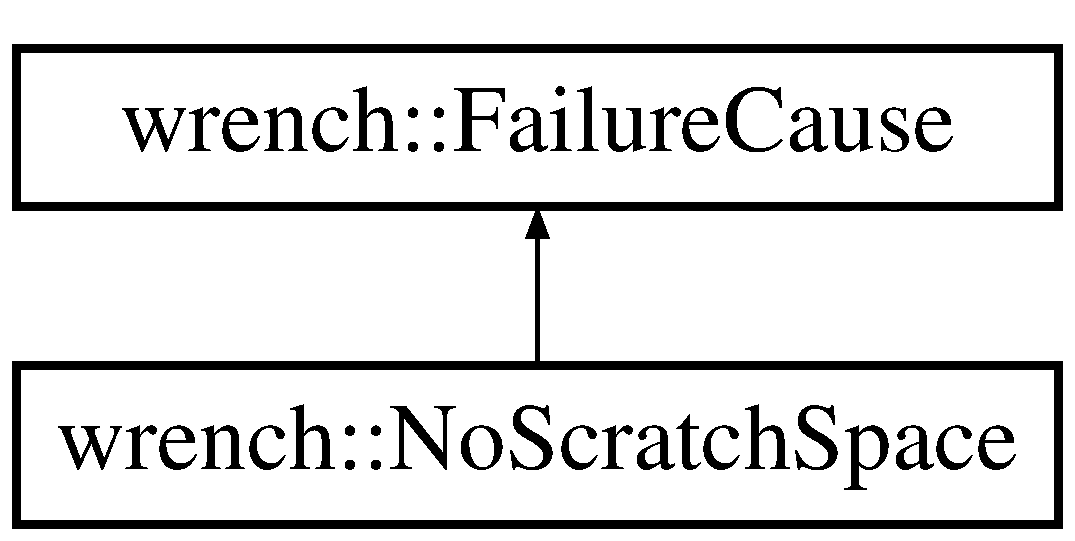
\includegraphics[height=2.000000cm]{classwrench_1_1_no_scratch_space}
\end{center}
\end{figure}
\subsection*{Public Member Functions}
\begin{DoxyCompactItemize}
\item 
\hyperlink{classwrench_1_1_no_scratch_space_a42f786f73e3ddce5921b90a6da828804}{No\+Scratch\+Space} (std\+::string error)
\begin{DoxyCompactList}\small\item\em Constructor. \end{DoxyCompactList}\item 
std\+::string \hyperlink{classwrench_1_1_no_scratch_space_add628f91104786a99a410ec07abac54c}{to\+String} ()
\begin{DoxyCompactList}\small\item\em Get the human-\/readable failure message. \end{DoxyCompactList}\end{DoxyCompactItemize}
\subsection*{Additional Inherited Members}


\subsection{Detailed Description}
A \char`\"{}no scratch space\char`\"{} failure cause. 

\subsection{Constructor \& Destructor Documentation}
\mbox{\Hypertarget{classwrench_1_1_no_scratch_space_a42f786f73e3ddce5921b90a6da828804}\label{classwrench_1_1_no_scratch_space_a42f786f73e3ddce5921b90a6da828804}} 
\index{wrench\+::\+No\+Scratch\+Space@{wrench\+::\+No\+Scratch\+Space}!No\+Scratch\+Space@{No\+Scratch\+Space}}
\index{No\+Scratch\+Space@{No\+Scratch\+Space}!wrench\+::\+No\+Scratch\+Space@{wrench\+::\+No\+Scratch\+Space}}
\subsubsection{\texorpdfstring{No\+Scratch\+Space()}{NoScratchSpace()}}
{\footnotesize\ttfamily wrench\+::\+No\+Scratch\+Space\+::\+No\+Scratch\+Space (\begin{DoxyParamCaption}\item[{std\+::string}]{error }\end{DoxyParamCaption})}



Constructor. 


\begin{DoxyParams}{Parameters}
{\em error} & error message \\
\hline
\end{DoxyParams}


\subsection{Member Function Documentation}
\mbox{\Hypertarget{classwrench_1_1_no_scratch_space_add628f91104786a99a410ec07abac54c}\label{classwrench_1_1_no_scratch_space_add628f91104786a99a410ec07abac54c}} 
\index{wrench\+::\+No\+Scratch\+Space@{wrench\+::\+No\+Scratch\+Space}!to\+String@{to\+String}}
\index{to\+String@{to\+String}!wrench\+::\+No\+Scratch\+Space@{wrench\+::\+No\+Scratch\+Space}}
\subsubsection{\texorpdfstring{to\+String()}{toString()}}
{\footnotesize\ttfamily std\+::string wrench\+::\+No\+Scratch\+Space\+::to\+String (\begin{DoxyParamCaption}{ }\end{DoxyParamCaption})\hspace{0.3cm}{\ttfamily [virtual]}}



Get the human-\/readable failure message. 

\begin{DoxyReturn}{Returns}
the message 
\end{DoxyReturn}


Implements \hyperlink{classwrench_1_1_failure_cause_afbad248ebe902409f2cd4f1d6f2b867d}{wrench\+::\+Failure\+Cause}.



The documentation for this class was generated from the following files\+:\begin{DoxyCompactItemize}
\item 
/\+Users/rafsilva/\+Documents/isi/workspace/wrench/wrench/include/wrench/workflow/execution\+\_\+events/Failure\+Cause.\+h\item 
/\+Users/rafsilva/\+Documents/isi/workspace/wrench/wrench/src/wrench/workflow/execution\+\_\+events/Failure\+Cause.\+cpp\end{DoxyCompactItemize}

\hypertarget{classwrench_1_1_no_storage_service_for_file}{}\section{wrench\+:\+:No\+Storage\+Service\+For\+File Class Reference}
\label{classwrench_1_1_no_storage_service_for_file}\index{wrench\+::\+No\+Storage\+Service\+For\+File@{wrench\+::\+No\+Storage\+Service\+For\+File}}


A \char`\"{}file cannot be found anywhere\char`\"{} failure cause.  




{\ttfamily \#include $<$Failure\+Cause.\+h$>$}

Inheritance diagram for wrench\+:\+:No\+Storage\+Service\+For\+File\+:\begin{figure}[H]
\begin{center}
\leavevmode
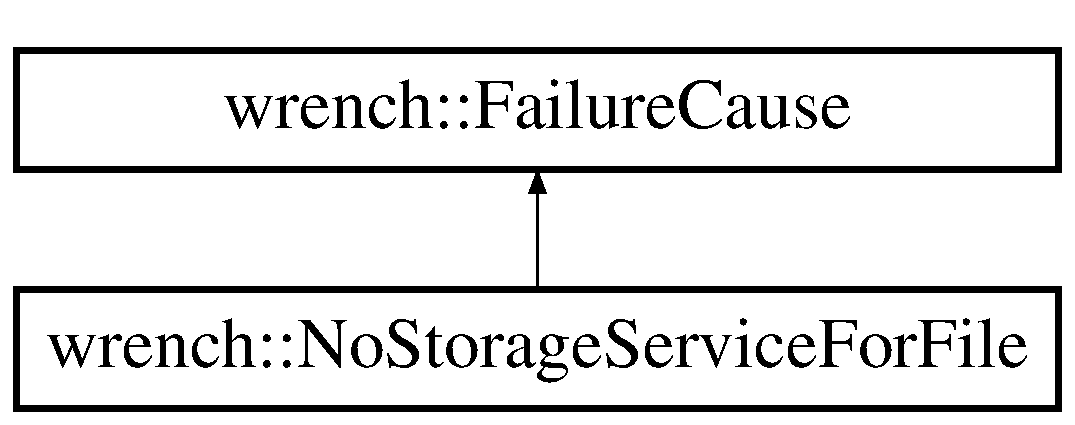
\includegraphics[height=2.000000cm]{classwrench_1_1_no_storage_service_for_file}
\end{center}
\end{figure}
\subsection*{Public Member Functions}
\begin{DoxyCompactItemize}
\item 
\hyperlink{classwrench_1_1_workflow_file}{Workflow\+File} $\ast$ \hyperlink{classwrench_1_1_no_storage_service_for_file_a0f9c9e16bac0150881b4303385b716a0}{get\+File} ()
\begin{DoxyCompactList}\small\item\em Getter. \end{DoxyCompactList}\item 
std\+::string \hyperlink{classwrench_1_1_no_storage_service_for_file_ab3941ca284f35abd00e9292e22d7d553}{to\+String} ()
\begin{DoxyCompactList}\small\item\em Get the human-\/readable failure message. \end{DoxyCompactList}\end{DoxyCompactItemize}
\subsection*{Additional Inherited Members}


\subsection{Detailed Description}
A \char`\"{}file cannot be found anywhere\char`\"{} failure cause. 

\subsection{Member Function Documentation}
\mbox{\Hypertarget{classwrench_1_1_no_storage_service_for_file_a0f9c9e16bac0150881b4303385b716a0}\label{classwrench_1_1_no_storage_service_for_file_a0f9c9e16bac0150881b4303385b716a0}} 
\index{wrench\+::\+No\+Storage\+Service\+For\+File@{wrench\+::\+No\+Storage\+Service\+For\+File}!get\+File@{get\+File}}
\index{get\+File@{get\+File}!wrench\+::\+No\+Storage\+Service\+For\+File@{wrench\+::\+No\+Storage\+Service\+For\+File}}
\subsubsection{\texorpdfstring{get\+File()}{getFile()}}
{\footnotesize\ttfamily \hyperlink{classwrench_1_1_workflow_file}{Workflow\+File} $\ast$ wrench\+::\+No\+Storage\+Service\+For\+File\+::get\+File (\begin{DoxyParamCaption}{ }\end{DoxyParamCaption})}



Getter. 

\begin{DoxyReturn}{Returns}
the file 
\end{DoxyReturn}
\mbox{\Hypertarget{classwrench_1_1_no_storage_service_for_file_ab3941ca284f35abd00e9292e22d7d553}\label{classwrench_1_1_no_storage_service_for_file_ab3941ca284f35abd00e9292e22d7d553}} 
\index{wrench\+::\+No\+Storage\+Service\+For\+File@{wrench\+::\+No\+Storage\+Service\+For\+File}!to\+String@{to\+String}}
\index{to\+String@{to\+String}!wrench\+::\+No\+Storage\+Service\+For\+File@{wrench\+::\+No\+Storage\+Service\+For\+File}}
\subsubsection{\texorpdfstring{to\+String()}{toString()}}
{\footnotesize\ttfamily std\+::string wrench\+::\+No\+Storage\+Service\+For\+File\+::to\+String (\begin{DoxyParamCaption}{ }\end{DoxyParamCaption})\hspace{0.3cm}{\ttfamily [virtual]}}



Get the human-\/readable failure message. 

\begin{DoxyReturn}{Returns}
the message 
\end{DoxyReturn}


Implements \hyperlink{classwrench_1_1_failure_cause_afbad248ebe902409f2cd4f1d6f2b867d}{wrench\+::\+Failure\+Cause}.



The documentation for this class was generated from the following files\+:\begin{DoxyCompactItemize}
\item 
/\+Users/rafsilva/\+Documents/isi/workspace/wrench/wrench/include/wrench/workflow/execution\+\_\+events/Failure\+Cause.\+h\item 
/\+Users/rafsilva/\+Documents/isi/workspace/wrench/wrench/src/wrench/workflow/execution\+\_\+events/Failure\+Cause.\+cpp\end{DoxyCompactItemize}

\hypertarget{classwrench_1_1_not_enough_resources}{}\section{wrench\+:\+:Not\+Enough\+Resources Class Reference}
\label{classwrench_1_1_not_enough_resources}\index{wrench\+::\+Not\+Enough\+Resources@{wrench\+::\+Not\+Enough\+Resources}}


A \char`\"{}compute service doesn\textquotesingle{}t have enough cores\char`\"{} failure cause.  




{\ttfamily \#include $<$Failure\+Cause.\+h$>$}

Inheritance diagram for wrench\+:\+:Not\+Enough\+Resources\+:\begin{figure}[H]
\begin{center}
\leavevmode
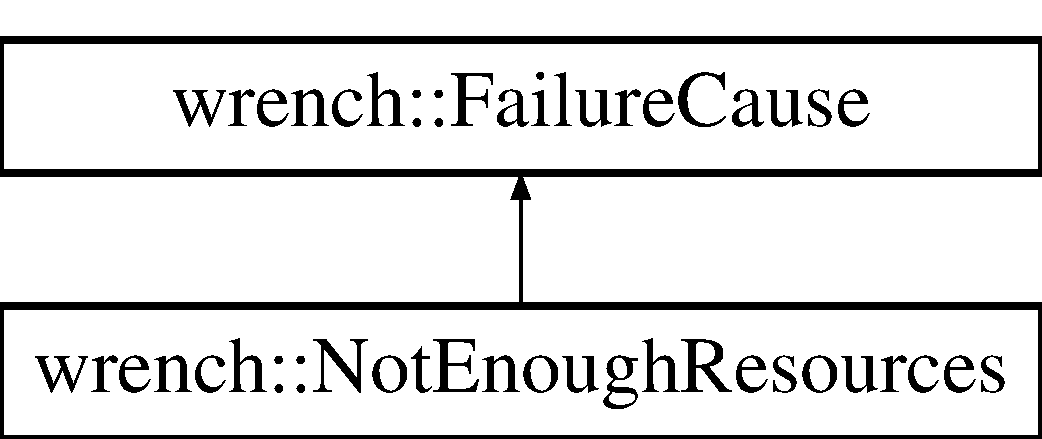
\includegraphics[height=2.000000cm]{classwrench_1_1_not_enough_resources}
\end{center}
\end{figure}
\subsection*{Public Member Functions}
\begin{DoxyCompactItemize}
\item 
\hyperlink{classwrench_1_1_not_enough_resources_a3ed2fb3a0726d4072ffed8c91521fda4}{Not\+Enough\+Resources} (\hyperlink{classwrench_1_1_workflow_job}{Workflow\+Job} $\ast$job, \hyperlink{classwrench_1_1_compute_service}{Compute\+Service} $\ast$compute\+\_\+service)
\begin{DoxyCompactList}\small\item\em Constructor. \end{DoxyCompactList}\item 
\hyperlink{classwrench_1_1_compute_service}{Compute\+Service} $\ast$ \hyperlink{classwrench_1_1_not_enough_resources_a2ded283721b584804b1220b2db4548b3}{get\+Compute\+Service} ()
\begin{DoxyCompactList}\small\item\em Getter. \end{DoxyCompactList}\item 
\hyperlink{classwrench_1_1_workflow_job}{Workflow\+Job} $\ast$ \hyperlink{classwrench_1_1_not_enough_resources_a8bf50edc9be82619b404ae82a9288f94}{get\+Job} ()
\begin{DoxyCompactList}\small\item\em Getter. \end{DoxyCompactList}\item 
std\+::string \hyperlink{classwrench_1_1_not_enough_resources_aeccad36aeccb259ac4c2d17752963269}{to\+String} ()
\begin{DoxyCompactList}\small\item\em Get the human-\/readable failure message. \end{DoxyCompactList}\end{DoxyCompactItemize}
\subsection*{Additional Inherited Members}


\subsection{Detailed Description}
A \char`\"{}compute service doesn\textquotesingle{}t have enough cores\char`\"{} failure cause. 

\subsection{Constructor \& Destructor Documentation}
\mbox{\Hypertarget{classwrench_1_1_not_enough_resources_a3ed2fb3a0726d4072ffed8c91521fda4}\label{classwrench_1_1_not_enough_resources_a3ed2fb3a0726d4072ffed8c91521fda4}} 
\index{wrench\+::\+Not\+Enough\+Resources@{wrench\+::\+Not\+Enough\+Resources}!Not\+Enough\+Resources@{Not\+Enough\+Resources}}
\index{Not\+Enough\+Resources@{Not\+Enough\+Resources}!wrench\+::\+Not\+Enough\+Resources@{wrench\+::\+Not\+Enough\+Resources}}
\subsubsection{\texorpdfstring{Not\+Enough\+Resources()}{NotEnoughResources()}}
{\footnotesize\ttfamily wrench\+::\+Not\+Enough\+Resources\+::\+Not\+Enough\+Resources (\begin{DoxyParamCaption}\item[{\hyperlink{classwrench_1_1_workflow_job}{Workflow\+Job} $\ast$}]{job,  }\item[{\hyperlink{classwrench_1_1_compute_service}{Compute\+Service} $\ast$}]{compute\+\_\+service }\end{DoxyParamCaption})}



Constructor. 


\begin{DoxyParams}{Parameters}
{\em job} & the job that could not be executed \\
\hline
{\em compute\+\_\+service} & the compute service that didn\textquotesingle{}t have enough cores or ram \\
\hline
\end{DoxyParams}


\subsection{Member Function Documentation}
\mbox{\Hypertarget{classwrench_1_1_not_enough_resources_a2ded283721b584804b1220b2db4548b3}\label{classwrench_1_1_not_enough_resources_a2ded283721b584804b1220b2db4548b3}} 
\index{wrench\+::\+Not\+Enough\+Resources@{wrench\+::\+Not\+Enough\+Resources}!get\+Compute\+Service@{get\+Compute\+Service}}
\index{get\+Compute\+Service@{get\+Compute\+Service}!wrench\+::\+Not\+Enough\+Resources@{wrench\+::\+Not\+Enough\+Resources}}
\subsubsection{\texorpdfstring{get\+Compute\+Service()}{getComputeService()}}
{\footnotesize\ttfamily \hyperlink{classwrench_1_1_compute_service}{Compute\+Service} $\ast$ wrench\+::\+Not\+Enough\+Resources\+::get\+Compute\+Service (\begin{DoxyParamCaption}{ }\end{DoxyParamCaption})}



Getter. 

\begin{DoxyReturn}{Returns}
the compute service 
\end{DoxyReturn}
\mbox{\Hypertarget{classwrench_1_1_not_enough_resources_a8bf50edc9be82619b404ae82a9288f94}\label{classwrench_1_1_not_enough_resources_a8bf50edc9be82619b404ae82a9288f94}} 
\index{wrench\+::\+Not\+Enough\+Resources@{wrench\+::\+Not\+Enough\+Resources}!get\+Job@{get\+Job}}
\index{get\+Job@{get\+Job}!wrench\+::\+Not\+Enough\+Resources@{wrench\+::\+Not\+Enough\+Resources}}
\subsubsection{\texorpdfstring{get\+Job()}{getJob()}}
{\footnotesize\ttfamily \hyperlink{classwrench_1_1_workflow_job}{Workflow\+Job} $\ast$ wrench\+::\+Not\+Enough\+Resources\+::get\+Job (\begin{DoxyParamCaption}{ }\end{DoxyParamCaption})}



Getter. 

\begin{DoxyReturn}{Returns}
the job 
\end{DoxyReturn}
\mbox{\Hypertarget{classwrench_1_1_not_enough_resources_aeccad36aeccb259ac4c2d17752963269}\label{classwrench_1_1_not_enough_resources_aeccad36aeccb259ac4c2d17752963269}} 
\index{wrench\+::\+Not\+Enough\+Resources@{wrench\+::\+Not\+Enough\+Resources}!to\+String@{to\+String}}
\index{to\+String@{to\+String}!wrench\+::\+Not\+Enough\+Resources@{wrench\+::\+Not\+Enough\+Resources}}
\subsubsection{\texorpdfstring{to\+String()}{toString()}}
{\footnotesize\ttfamily std\+::string wrench\+::\+Not\+Enough\+Resources\+::to\+String (\begin{DoxyParamCaption}{ }\end{DoxyParamCaption})\hspace{0.3cm}{\ttfamily [virtual]}}



Get the human-\/readable failure message. 

\begin{DoxyReturn}{Returns}
the message 
\end{DoxyReturn}


Implements \hyperlink{classwrench_1_1_failure_cause_afbad248ebe902409f2cd4f1d6f2b867d}{wrench\+::\+Failure\+Cause}.



The documentation for this class was generated from the following files\+:\begin{DoxyCompactItemize}
\item 
/\+Users/rafsilva/\+Documents/isi/workspace/wrench/wrench/include/wrench/workflow/execution\+\_\+events/Failure\+Cause.\+h\item 
/\+Users/rafsilva/\+Documents/isi/workspace/wrench/wrench/src/wrench/workflow/execution\+\_\+events/Failure\+Cause.\+cpp\end{DoxyCompactItemize}

\hypertarget{classwrench_1_1_pilot_job}{}\section{wrench\+:\+:Pilot\+Job Class Reference}
\label{classwrench_1_1_pilot_job}\index{wrench\+::\+Pilot\+Job@{wrench\+::\+Pilot\+Job}}


A pilot (i.\+e., non-\/standard) workflow job that can be submitted to a \hyperlink{classwrench_1_1_compute_service}{Compute\+Service} by a \hyperlink{classwrench_1_1_w_m_s}{W\+MS} (via a \hyperlink{classwrench_1_1_job_manager}{Job\+Manager})  




{\ttfamily \#include $<$Pilot\+Job.\+h$>$}

Inheritance diagram for wrench\+:\+:Pilot\+Job\+:\begin{figure}[H]
\begin{center}
\leavevmode
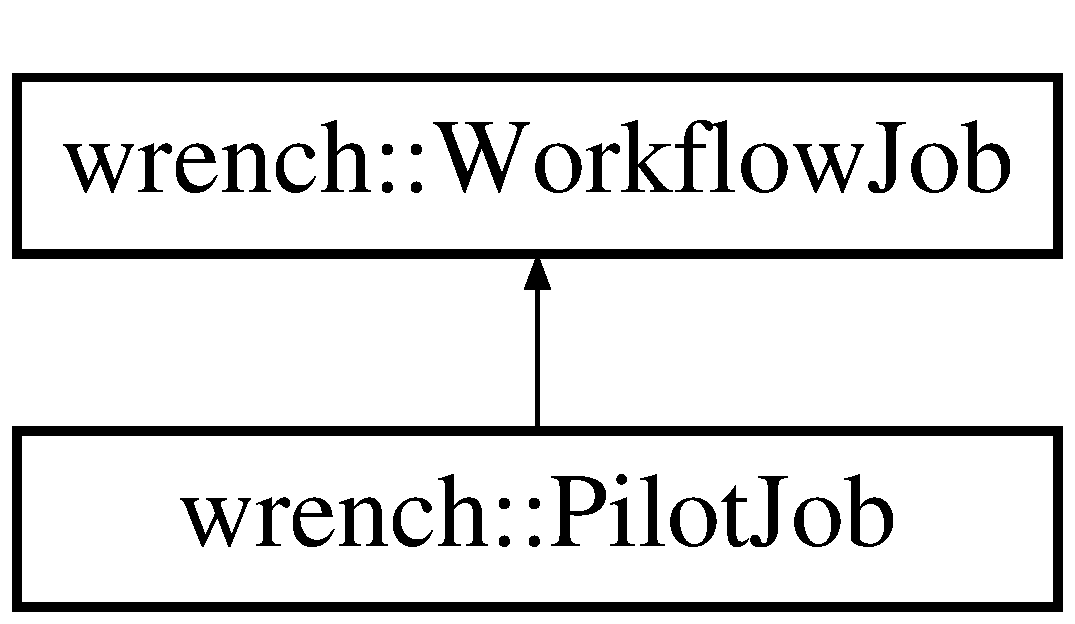
\includegraphics[height=2.000000cm]{classwrench_1_1_pilot_job}
\end{center}
\end{figure}
\subsection*{Public Types}
\begin{DoxyCompactItemize}
\item 
enum \hyperlink{classwrench_1_1_pilot_job_a0540139dbc8b0a8506a87b2f55020fc8}{State} \{ \newline
\hyperlink{classwrench_1_1_pilot_job_a0540139dbc8b0a8506a87b2f55020fc8abb71dfcf76439732a0744de5ff4af302}{N\+O\+T\+\_\+\+S\+U\+B\+M\+I\+T\+T\+ED}, 
\hyperlink{classwrench_1_1_pilot_job_a0540139dbc8b0a8506a87b2f55020fc8ad580f9552e724bb04d8ce76b1577efa9}{P\+E\+N\+D\+I\+NG}, 
\hyperlink{classwrench_1_1_pilot_job_a0540139dbc8b0a8506a87b2f55020fc8a3b9c4d0ba8d77eceba1375e5a45f0f78}{R\+U\+N\+N\+I\+NG}, 
\hyperlink{classwrench_1_1_pilot_job_a0540139dbc8b0a8506a87b2f55020fc8adb2cdc68dca41bf37d4e7e2703010381}{E\+X\+P\+I\+R\+ED}, 
\newline
\hyperlink{classwrench_1_1_pilot_job_a0540139dbc8b0a8506a87b2f55020fc8ac3e5bd2baec9dd138ff1bd886b801950}{F\+A\+I\+L\+ED}, 
\hyperlink{classwrench_1_1_pilot_job_a0540139dbc8b0a8506a87b2f55020fc8a21352143c29095d065e7a042b5dc453c}{T\+E\+R\+M\+I\+N\+A\+T\+ED}
 \}\begin{DoxyCompactList}\small\item\em Pilot job states. \end{DoxyCompactList}
\end{DoxyCompactItemize}
\subsection*{Public Member Functions}
\begin{DoxyCompactItemize}
\item 
\hyperlink{classwrench_1_1_compute_service}{Compute\+Service} $\ast$ \hyperlink{classwrench_1_1_pilot_job_a296881f5e960313121e9cba4b89a1e9c}{get\+Compute\+Service} ()
\begin{DoxyCompactList}\small\item\em Get the compute service provided by the (running) pilot job. \end{DoxyCompactList}\item 
\hyperlink{classwrench_1_1_pilot_job_a0540139dbc8b0a8506a87b2f55020fc8}{Pilot\+Job\+::\+State} \hyperlink{classwrench_1_1_pilot_job_a3890ff3cb3b494270c7a635748c91d95}{get\+State} ()
\begin{DoxyCompactList}\small\item\em Get the state of the pilot job. \end{DoxyCompactList}\end{DoxyCompactItemize}


\subsection{Detailed Description}
A pilot (i.\+e., non-\/standard) workflow job that can be submitted to a \hyperlink{classwrench_1_1_compute_service}{Compute\+Service} by a \hyperlink{classwrench_1_1_w_m_s}{W\+MS} (via a \hyperlink{classwrench_1_1_job_manager}{Job\+Manager}) 

\subsection{Member Enumeration Documentation}
\mbox{\Hypertarget{classwrench_1_1_pilot_job_a0540139dbc8b0a8506a87b2f55020fc8}\label{classwrench_1_1_pilot_job_a0540139dbc8b0a8506a87b2f55020fc8}} 
\index{wrench\+::\+Pilot\+Job@{wrench\+::\+Pilot\+Job}!State@{State}}
\index{State@{State}!wrench\+::\+Pilot\+Job@{wrench\+::\+Pilot\+Job}}
\subsubsection{\texorpdfstring{State}{State}}
{\footnotesize\ttfamily enum \hyperlink{classwrench_1_1_pilot_job_a0540139dbc8b0a8506a87b2f55020fc8}{wrench\+::\+Pilot\+Job\+::\+State}}



Pilot job states. 

\begin{DoxyEnumFields}{Enumerator}
\raisebox{\heightof{T}}[0pt][0pt]{\index{N\+O\+T\+\_\+\+S\+U\+B\+M\+I\+T\+T\+ED@{N\+O\+T\+\_\+\+S\+U\+B\+M\+I\+T\+T\+ED}!wrench\+::\+Pilot\+Job@{wrench\+::\+Pilot\+Job}}\index{wrench\+::\+Pilot\+Job@{wrench\+::\+Pilot\+Job}!N\+O\+T\+\_\+\+S\+U\+B\+M\+I\+T\+T\+ED@{N\+O\+T\+\_\+\+S\+U\+B\+M\+I\+T\+T\+ED}}}\mbox{\Hypertarget{classwrench_1_1_pilot_job_a0540139dbc8b0a8506a87b2f55020fc8abb71dfcf76439732a0744de5ff4af302}\label{classwrench_1_1_pilot_job_a0540139dbc8b0a8506a87b2f55020fc8abb71dfcf76439732a0744de5ff4af302}} 
N\+O\+T\+\_\+\+S\+U\+B\+M\+I\+T\+T\+ED&Not submitted yet. \\
\hline

\raisebox{\heightof{T}}[0pt][0pt]{\index{P\+E\+N\+D\+I\+NG@{P\+E\+N\+D\+I\+NG}!wrench\+::\+Pilot\+Job@{wrench\+::\+Pilot\+Job}}\index{wrench\+::\+Pilot\+Job@{wrench\+::\+Pilot\+Job}!P\+E\+N\+D\+I\+NG@{P\+E\+N\+D\+I\+NG}}}\mbox{\Hypertarget{classwrench_1_1_pilot_job_a0540139dbc8b0a8506a87b2f55020fc8ad580f9552e724bb04d8ce76b1577efa9}\label{classwrench_1_1_pilot_job_a0540139dbc8b0a8506a87b2f55020fc8ad580f9552e724bb04d8ce76b1577efa9}} 
P\+E\+N\+D\+I\+NG&Submitted but not running. \\
\hline

\raisebox{\heightof{T}}[0pt][0pt]{\index{R\+U\+N\+N\+I\+NG@{R\+U\+N\+N\+I\+NG}!wrench\+::\+Pilot\+Job@{wrench\+::\+Pilot\+Job}}\index{wrench\+::\+Pilot\+Job@{wrench\+::\+Pilot\+Job}!R\+U\+N\+N\+I\+NG@{R\+U\+N\+N\+I\+NG}}}\mbox{\Hypertarget{classwrench_1_1_pilot_job_a0540139dbc8b0a8506a87b2f55020fc8a3b9c4d0ba8d77eceba1375e5a45f0f78}\label{classwrench_1_1_pilot_job_a0540139dbc8b0a8506a87b2f55020fc8a3b9c4d0ba8d77eceba1375e5a45f0f78}} 
R\+U\+N\+N\+I\+NG&Running. \\
\hline

\raisebox{\heightof{T}}[0pt][0pt]{\index{E\+X\+P\+I\+R\+ED@{E\+X\+P\+I\+R\+ED}!wrench\+::\+Pilot\+Job@{wrench\+::\+Pilot\+Job}}\index{wrench\+::\+Pilot\+Job@{wrench\+::\+Pilot\+Job}!E\+X\+P\+I\+R\+ED@{E\+X\+P\+I\+R\+ED}}}\mbox{\Hypertarget{classwrench_1_1_pilot_job_a0540139dbc8b0a8506a87b2f55020fc8adb2cdc68dca41bf37d4e7e2703010381}\label{classwrench_1_1_pilot_job_a0540139dbc8b0a8506a87b2f55020fc8adb2cdc68dca41bf37d4e7e2703010381}} 
E\+X\+P\+I\+R\+ED&Expired due to a time-\/to-\/live limit. \\
\hline

\raisebox{\heightof{T}}[0pt][0pt]{\index{F\+A\+I\+L\+ED@{F\+A\+I\+L\+ED}!wrench\+::\+Pilot\+Job@{wrench\+::\+Pilot\+Job}}\index{wrench\+::\+Pilot\+Job@{wrench\+::\+Pilot\+Job}!F\+A\+I\+L\+ED@{F\+A\+I\+L\+ED}}}\mbox{\Hypertarget{classwrench_1_1_pilot_job_a0540139dbc8b0a8506a87b2f55020fc8ac3e5bd2baec9dd138ff1bd886b801950}\label{classwrench_1_1_pilot_job_a0540139dbc8b0a8506a87b2f55020fc8ac3e5bd2baec9dd138ff1bd886b801950}} 
F\+A\+I\+L\+ED&Failed. \\
\hline

\raisebox{\heightof{T}}[0pt][0pt]{\index{T\+E\+R\+M\+I\+N\+A\+T\+ED@{T\+E\+R\+M\+I\+N\+A\+T\+ED}!wrench\+::\+Pilot\+Job@{wrench\+::\+Pilot\+Job}}\index{wrench\+::\+Pilot\+Job@{wrench\+::\+Pilot\+Job}!T\+E\+R\+M\+I\+N\+A\+T\+ED@{T\+E\+R\+M\+I\+N\+A\+T\+ED}}}\mbox{\Hypertarget{classwrench_1_1_pilot_job_a0540139dbc8b0a8506a87b2f55020fc8a21352143c29095d065e7a042b5dc453c}\label{classwrench_1_1_pilot_job_a0540139dbc8b0a8506a87b2f55020fc8a21352143c29095d065e7a042b5dc453c}} 
T\+E\+R\+M\+I\+N\+A\+T\+ED&Terminated by submitter. \\
\hline

\end{DoxyEnumFields}


\subsection{Member Function Documentation}
\mbox{\Hypertarget{classwrench_1_1_pilot_job_a296881f5e960313121e9cba4b89a1e9c}\label{classwrench_1_1_pilot_job_a296881f5e960313121e9cba4b89a1e9c}} 
\index{wrench\+::\+Pilot\+Job@{wrench\+::\+Pilot\+Job}!get\+Compute\+Service@{get\+Compute\+Service}}
\index{get\+Compute\+Service@{get\+Compute\+Service}!wrench\+::\+Pilot\+Job@{wrench\+::\+Pilot\+Job}}
\subsubsection{\texorpdfstring{get\+Compute\+Service()}{getComputeService()}}
{\footnotesize\ttfamily \hyperlink{classwrench_1_1_compute_service}{Compute\+Service} $\ast$ wrench\+::\+Pilot\+Job\+::get\+Compute\+Service (\begin{DoxyParamCaption}{ }\end{DoxyParamCaption})}



Get the compute service provided by the (running) pilot job. 

\begin{DoxyReturn}{Returns}
a compute service 
\end{DoxyReturn}
\mbox{\Hypertarget{classwrench_1_1_pilot_job_a3890ff3cb3b494270c7a635748c91d95}\label{classwrench_1_1_pilot_job_a3890ff3cb3b494270c7a635748c91d95}} 
\index{wrench\+::\+Pilot\+Job@{wrench\+::\+Pilot\+Job}!get\+State@{get\+State}}
\index{get\+State@{get\+State}!wrench\+::\+Pilot\+Job@{wrench\+::\+Pilot\+Job}}
\subsubsection{\texorpdfstring{get\+State()}{getState()}}
{\footnotesize\ttfamily \hyperlink{classwrench_1_1_pilot_job_a0540139dbc8b0a8506a87b2f55020fc8}{Pilot\+Job\+::\+State} wrench\+::\+Pilot\+Job\+::get\+State (\begin{DoxyParamCaption}{ }\end{DoxyParamCaption})}



Get the state of the pilot job. 

\begin{DoxyReturn}{Returns}
the state 
\end{DoxyReturn}


The documentation for this class was generated from the following files\+:\begin{DoxyCompactItemize}
\item 
/\+Users/rafsilva/\+Documents/isi/workspace/wrench/wrench/include/wrench/workflow/job/Pilot\+Job.\+h\item 
/\+Users/rafsilva/\+Documents/isi/workspace/wrench/wrench/src/wrench/workflow/job/Pilot\+Job.\+cpp\end{DoxyCompactItemize}

\hypertarget{classwrench_1_1_pilot_job_expired_event}{}\section{wrench\+:\+:Pilot\+Job\+Expired\+Event Class Reference}
\label{classwrench_1_1_pilot_job_expired_event}\index{wrench\+::\+Pilot\+Job\+Expired\+Event@{wrench\+::\+Pilot\+Job\+Expired\+Event}}


A \char`\"{}pilot job has expired\char`\"{} \hyperlink{classwrench_1_1_workflow_execution_event}{Workflow\+Execution\+Event}.  




{\ttfamily \#include $<$Workflow\+Execution\+Event.\+h$>$}

Inheritance diagram for wrench\+:\+:Pilot\+Job\+Expired\+Event\+:\begin{figure}[H]
\begin{center}
\leavevmode
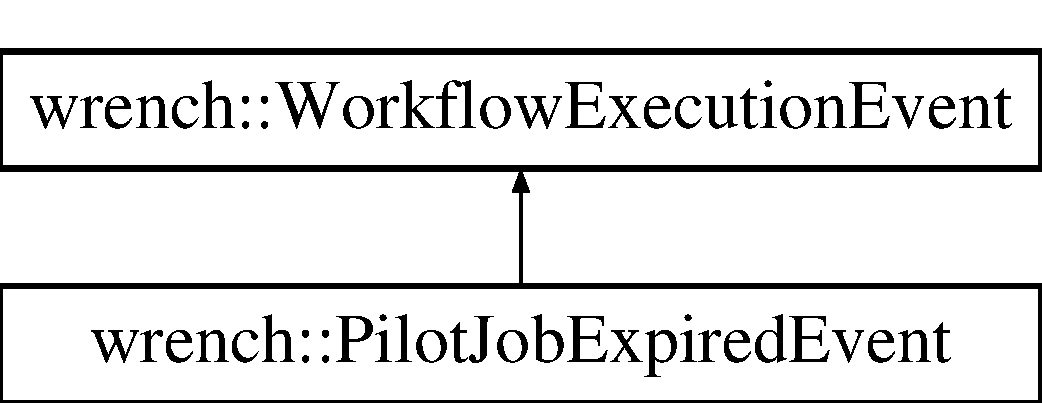
\includegraphics[height=2.000000cm]{classwrench_1_1_pilot_job_expired_event}
\end{center}
\end{figure}
\subsection*{Public Attributes}
\begin{DoxyCompactItemize}
\item 
\mbox{\Hypertarget{classwrench_1_1_pilot_job_expired_event_aebbb89a30b8f24f1c7866df191293e7b}\label{classwrench_1_1_pilot_job_expired_event_aebbb89a30b8f24f1c7866df191293e7b}} 
\hyperlink{classwrench_1_1_compute_service}{Compute\+Service} $\ast$ \hyperlink{classwrench_1_1_pilot_job_expired_event_aebbb89a30b8f24f1c7866df191293e7b}{compute\+\_\+service}
\begin{DoxyCompactList}\small\item\em The compute service on which the pilot job has expired. \end{DoxyCompactList}\item 
\mbox{\Hypertarget{classwrench_1_1_pilot_job_expired_event_a049f2f444c6185e9346173253f3b2a21}\label{classwrench_1_1_pilot_job_expired_event_a049f2f444c6185e9346173253f3b2a21}} 
\hyperlink{classwrench_1_1_pilot_job}{Pilot\+Job} $\ast$ \hyperlink{classwrench_1_1_pilot_job_expired_event_a049f2f444c6185e9346173253f3b2a21}{pilot\+\_\+job}
\begin{DoxyCompactList}\small\item\em The pilot job that has expired. \end{DoxyCompactList}\end{DoxyCompactItemize}
\subsection*{Additional Inherited Members}


\subsection{Detailed Description}
A \char`\"{}pilot job has expired\char`\"{} \hyperlink{classwrench_1_1_workflow_execution_event}{Workflow\+Execution\+Event}. 

The documentation for this class was generated from the following file\+:\begin{DoxyCompactItemize}
\item 
/\+Users/rafsilva/\+Documents/isi/workspace/wrench/wrench/include/wrench/workflow/execution\+\_\+events/Workflow\+Execution\+Event.\+h\end{DoxyCompactItemize}

\hypertarget{classwrench_1_1_pilot_job_scheduler}{}\section{wrench\+:\+:Pilot\+Job\+Scheduler Class Reference}
\label{classwrench_1_1_pilot_job_scheduler}\index{wrench\+::\+Pilot\+Job\+Scheduler@{wrench\+::\+Pilot\+Job\+Scheduler}}


A (mostly virtual) base class for implementing \hyperlink{classwrench_1_1_pilot_job}{Pilot\+Job} scheduling algorithms to be used by a \hyperlink{classwrench_1_1_w_m_s}{W\+MS}.  




{\ttfamily \#include $<$Pilot\+Job\+Scheduler.\+h$>$}

\subsection*{Public Member Functions}
\begin{DoxyCompactItemize}
\item 
\mbox{\Hypertarget{classwrench_1_1_pilot_job_scheduler_ab230034aa98439169dc78bcf82bfced8}\label{classwrench_1_1_pilot_job_scheduler_ab230034aa98439169dc78bcf82bfced8}} 
\hyperlink{classwrench_1_1_pilot_job_scheduler_ab230034aa98439169dc78bcf82bfced8}{Pilot\+Job\+Scheduler} ()
\begin{DoxyCompactList}\small\item\em Constructor. \end{DoxyCompactList}\item 
\hyperlink{classwrench_1_1_data_movement_manager}{Data\+Movement\+Manager} $\ast$ \hyperlink{classwrench_1_1_pilot_job_scheduler_ab161a17fd3c1a7f5af171f813e32f3a1}{get\+Data\+Movement\+Manager} ()
\begin{DoxyCompactList}\small\item\em Get the data movement manager to be used by this scheduler (nullptr\+: none is used) \end{DoxyCompactList}\item 
\hyperlink{classwrench_1_1_job_manager}{Job\+Manager} $\ast$ \hyperlink{classwrench_1_1_pilot_job_scheduler_acd33b44c3481d911489626dc3f0ea957}{get\+Job\+Manager} ()
\begin{DoxyCompactList}\small\item\em Get the job manager to be used by this scheduler (nullptr\+: none is used) \end{DoxyCompactList}\item 
virtual void \hyperlink{classwrench_1_1_pilot_job_scheduler_a903c44145dfce2964f90cc856146adbb}{schedule\+Pilot\+Jobs} (const std\+::set$<$ \hyperlink{classwrench_1_1_compute_service}{Compute\+Service} $\ast$$>$ \&compute\+\_\+services)=0
\begin{DoxyCompactList}\small\item\em A method that schedules pilot jobs, according to whatever decision algorithm it implements, over a set of compute services. \end{DoxyCompactList}\end{DoxyCompactItemize}


\subsection{Detailed Description}
A (mostly virtual) base class for implementing \hyperlink{classwrench_1_1_pilot_job}{Pilot\+Job} scheduling algorithms to be used by a \hyperlink{classwrench_1_1_w_m_s}{W\+MS}. 

\subsection{Member Function Documentation}
\mbox{\Hypertarget{classwrench_1_1_pilot_job_scheduler_ab161a17fd3c1a7f5af171f813e32f3a1}\label{classwrench_1_1_pilot_job_scheduler_ab161a17fd3c1a7f5af171f813e32f3a1}} 
\index{wrench\+::\+Pilot\+Job\+Scheduler@{wrench\+::\+Pilot\+Job\+Scheduler}!get\+Data\+Movement\+Manager@{get\+Data\+Movement\+Manager}}
\index{get\+Data\+Movement\+Manager@{get\+Data\+Movement\+Manager}!wrench\+::\+Pilot\+Job\+Scheduler@{wrench\+::\+Pilot\+Job\+Scheduler}}
\subsubsection{\texorpdfstring{get\+Data\+Movement\+Manager()}{getDataMovementManager()}}
{\footnotesize\ttfamily \hyperlink{classwrench_1_1_data_movement_manager}{Data\+Movement\+Manager}$\ast$ wrench\+::\+Pilot\+Job\+Scheduler\+::get\+Data\+Movement\+Manager (\begin{DoxyParamCaption}{ }\end{DoxyParamCaption})\hspace{0.3cm}{\ttfamily [inline]}}



Get the data movement manager to be used by this scheduler (nullptr\+: none is used) 

\begin{DoxyReturn}{Returns}
a data movement manager 
\end{DoxyReturn}
\mbox{\Hypertarget{classwrench_1_1_pilot_job_scheduler_acd33b44c3481d911489626dc3f0ea957}\label{classwrench_1_1_pilot_job_scheduler_acd33b44c3481d911489626dc3f0ea957}} 
\index{wrench\+::\+Pilot\+Job\+Scheduler@{wrench\+::\+Pilot\+Job\+Scheduler}!get\+Job\+Manager@{get\+Job\+Manager}}
\index{get\+Job\+Manager@{get\+Job\+Manager}!wrench\+::\+Pilot\+Job\+Scheduler@{wrench\+::\+Pilot\+Job\+Scheduler}}
\subsubsection{\texorpdfstring{get\+Job\+Manager()}{getJobManager()}}
{\footnotesize\ttfamily \hyperlink{classwrench_1_1_job_manager}{Job\+Manager}$\ast$ wrench\+::\+Pilot\+Job\+Scheduler\+::get\+Job\+Manager (\begin{DoxyParamCaption}{ }\end{DoxyParamCaption})\hspace{0.3cm}{\ttfamily [inline]}}



Get the job manager to be used by this scheduler (nullptr\+: none is used) 

\begin{DoxyReturn}{Returns}
a job manager 
\end{DoxyReturn}
\mbox{\Hypertarget{classwrench_1_1_pilot_job_scheduler_a903c44145dfce2964f90cc856146adbb}\label{classwrench_1_1_pilot_job_scheduler_a903c44145dfce2964f90cc856146adbb}} 
\index{wrench\+::\+Pilot\+Job\+Scheduler@{wrench\+::\+Pilot\+Job\+Scheduler}!schedule\+Pilot\+Jobs@{schedule\+Pilot\+Jobs}}
\index{schedule\+Pilot\+Jobs@{schedule\+Pilot\+Jobs}!wrench\+::\+Pilot\+Job\+Scheduler@{wrench\+::\+Pilot\+Job\+Scheduler}}
\subsubsection{\texorpdfstring{schedule\+Pilot\+Jobs()}{schedulePilotJobs()}}
{\footnotesize\ttfamily virtual void wrench\+::\+Pilot\+Job\+Scheduler\+::schedule\+Pilot\+Jobs (\begin{DoxyParamCaption}\item[{const std\+::set$<$ \hyperlink{classwrench_1_1_compute_service}{Compute\+Service} $\ast$$>$ \&}]{compute\+\_\+services }\end{DoxyParamCaption})\hspace{0.3cm}{\ttfamily [pure virtual]}}



A method that schedules pilot jobs, according to whatever decision algorithm it implements, over a set of compute services. 


\begin{DoxyParams}{Parameters}
{\em compute\+\_\+services} & the set of compute services \\
\hline
\end{DoxyParams}


The documentation for this class was generated from the following file\+:\begin{DoxyCompactItemize}
\item 
/\+Users/rafsilva/\+Documents/isi/workspace/wrench/wrench/include/wrench/wms/scheduler/Pilot\+Job\+Scheduler.\+h\end{DoxyCompactItemize}

\hypertarget{classwrench_1_1_pilot_job_started_event}{}\section{wrench\+:\+:Pilot\+Job\+Started\+Event Class Reference}
\label{classwrench_1_1_pilot_job_started_event}\index{wrench\+::\+Pilot\+Job\+Started\+Event@{wrench\+::\+Pilot\+Job\+Started\+Event}}


A \char`\"{}pilot job has started\char`\"{} \hyperlink{classwrench_1_1_workflow_execution_event}{Workflow\+Execution\+Event}.  




{\ttfamily \#include $<$Workflow\+Execution\+Event.\+h$>$}

Inheritance diagram for wrench\+:\+:Pilot\+Job\+Started\+Event\+:\begin{figure}[H]
\begin{center}
\leavevmode
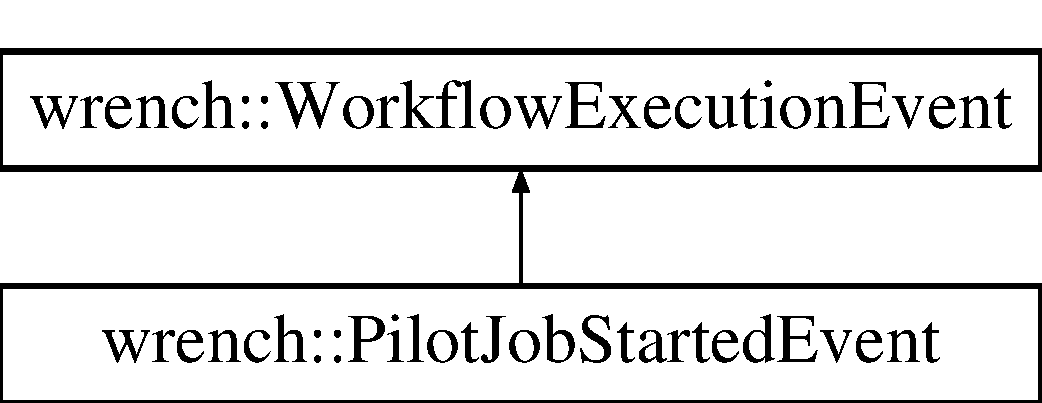
\includegraphics[height=2.000000cm]{classwrench_1_1_pilot_job_started_event}
\end{center}
\end{figure}
\subsection*{Public Attributes}
\begin{DoxyCompactItemize}
\item 
\mbox{\Hypertarget{classwrench_1_1_pilot_job_started_event_a761239b10cbab789c1fbead4aaa3ee34}\label{classwrench_1_1_pilot_job_started_event_a761239b10cbab789c1fbead4aaa3ee34}} 
\hyperlink{classwrench_1_1_compute_service}{Compute\+Service} $\ast$ \hyperlink{classwrench_1_1_pilot_job_started_event_a761239b10cbab789c1fbead4aaa3ee34}{compute\+\_\+service}
\begin{DoxyCompactList}\small\item\em The compute service on which the pilot job has started. \end{DoxyCompactList}\item 
\mbox{\Hypertarget{classwrench_1_1_pilot_job_started_event_ac5415bb05bddcf669164022d88b92475}\label{classwrench_1_1_pilot_job_started_event_ac5415bb05bddcf669164022d88b92475}} 
\hyperlink{classwrench_1_1_pilot_job}{Pilot\+Job} $\ast$ \hyperlink{classwrench_1_1_pilot_job_started_event_ac5415bb05bddcf669164022d88b92475}{pilot\+\_\+job}
\begin{DoxyCompactList}\small\item\em The pilot job that has started. \end{DoxyCompactList}\end{DoxyCompactItemize}
\subsection*{Additional Inherited Members}


\subsection{Detailed Description}
A \char`\"{}pilot job has started\char`\"{} \hyperlink{classwrench_1_1_workflow_execution_event}{Workflow\+Execution\+Event}. 

The documentation for this class was generated from the following file\+:\begin{DoxyCompactItemize}
\item 
/\+Users/rafsilva/\+Documents/isi/workspace/wrench/wrench/include/wrench/workflow/execution\+\_\+events/Workflow\+Execution\+Event.\+h\end{DoxyCompactItemize}

\hypertarget{classwrench_1_1_service}{}\section{wrench\+:\+:Service Class Reference}
\label{classwrench_1_1_service}\index{wrench\+::\+Service@{wrench\+::\+Service}}


A service that can be added to the simulation and that can be used by a \hyperlink{classwrench_1_1_w_m_s}{W\+MS} when executing a workflow.  




{\ttfamily \#include $<$Service.\+h$>$}

Inheritance diagram for wrench\+:\+:Service\+:\begin{figure}[H]
\begin{center}
\leavevmode
\includegraphics[height=1.187447cm]{classwrench_1_1_service}
\end{center}
\end{figure}


\subsection{Detailed Description}
A service that can be added to the simulation and that can be used by a \hyperlink{classwrench_1_1_w_m_s}{W\+MS} when executing a workflow. 

The documentation for this class was generated from the following file\+:\begin{DoxyCompactItemize}
\item 
/\+Users/rafsilva/\+Documents/isi/workspace/wrench/wrench/include/wrench/services/Service.\+h\end{DoxyCompactItemize}

\hypertarget{classwrench_1_1_service_failure_detector}{}\section{wrench\+:\+:Service\+Failure\+Detector Class Reference}
\label{classwrench_1_1_service_failure_detector}\index{wrench\+::\+Service\+Failure\+Detector@{wrench\+::\+Service\+Failure\+Detector}}
Inheritance diagram for wrench\+:\+:Service\+Failure\+Detector\+:\begin{figure}[H]
\begin{center}
\leavevmode
\includegraphics[height=3.000000cm]{classwrench_1_1_service_failure_detector}
\end{center}
\end{figure}
\subsection*{Public Member Functions}
\begin{DoxyCompactItemize}
\item 
\mbox{\Hypertarget{classwrench_1_1_service_failure_detector_a8c90fc986c6061173c1db533f3d407d1}\label{classwrench_1_1_service_failure_detector_a8c90fc986c6061173c1db533f3d407d1}} 
{\bfseries Service\+Failure\+Detector} (std\+::string host\+\_\+on\+\_\+which\+\_\+to\+\_\+run, \hyperlink{classwrench_1_1_service}{Service} $\ast$service\+\_\+to\+\_\+monitor, std\+::string mailbox\+\_\+to\+\_\+notify)
\end{DoxyCompactItemize}


The documentation for this class was generated from the following files\+:\begin{DoxyCompactItemize}
\item 
/\+Users/rafsilva/\+Documents/isi/workspace/wrench/wrench/include/wrench/services/helpers/Service\+Failure\+Detector.\+h\item 
/\+Users/rafsilva/\+Documents/isi/workspace/wrench/wrench/src/wrench/services/helpers/Service\+Failure\+Detector.\+cpp\end{DoxyCompactItemize}

\hypertarget{classwrench_1_1_service_is_down}{}\section{wrench\+:\+:Service\+Is\+Down Class Reference}
\label{classwrench_1_1_service_is_down}\index{wrench\+::\+Service\+Is\+Down@{wrench\+::\+Service\+Is\+Down}}


A \char`\"{}service is down\char`\"{} failure cause.  




{\ttfamily \#include $<$Failure\+Cause.\+h$>$}

Inheritance diagram for wrench\+:\+:Service\+Is\+Down\+:\begin{figure}[H]
\begin{center}
\leavevmode
\includegraphics[height=2.000000cm]{classwrench_1_1_service_is_down}
\end{center}
\end{figure}
\subsection*{Public Member Functions}
\begin{DoxyCompactItemize}
\item 
\hyperlink{classwrench_1_1_service_is_down_aa126c61019d1c3131c8ac71454c30ef5}{Service\+Is\+Down} (\hyperlink{classwrench_1_1_service}{Service} $\ast$service)
\begin{DoxyCompactList}\small\item\em Constructor. \end{DoxyCompactList}\item 
\hyperlink{classwrench_1_1_service}{Service} $\ast$ \hyperlink{classwrench_1_1_service_is_down_a1e92883f2634958f1af834d791097c90}{get\+Service} ()
\begin{DoxyCompactList}\small\item\em Getter. \end{DoxyCompactList}\item 
std\+::string \hyperlink{classwrench_1_1_service_is_down_a29dbb2d3dd1b5d6a47536bab974b7151}{to\+String} () override
\begin{DoxyCompactList}\small\item\em Get the human-\/readable failure message. \end{DoxyCompactList}\end{DoxyCompactItemize}
\subsection*{Additional Inherited Members}


\subsection{Detailed Description}
A \char`\"{}service is down\char`\"{} failure cause. 

\subsection{Constructor \& Destructor Documentation}
\mbox{\Hypertarget{classwrench_1_1_service_is_down_aa126c61019d1c3131c8ac71454c30ef5}\label{classwrench_1_1_service_is_down_aa126c61019d1c3131c8ac71454c30ef5}} 
\index{wrench\+::\+Service\+Is\+Down@{wrench\+::\+Service\+Is\+Down}!Service\+Is\+Down@{Service\+Is\+Down}}
\index{Service\+Is\+Down@{Service\+Is\+Down}!wrench\+::\+Service\+Is\+Down@{wrench\+::\+Service\+Is\+Down}}
\subsubsection{\texorpdfstring{Service\+Is\+Down()}{ServiceIsDown()}}
{\footnotesize\ttfamily wrench\+::\+Service\+Is\+Down\+::\+Service\+Is\+Down (\begin{DoxyParamCaption}\item[{\hyperlink{classwrench_1_1_service}{Service} $\ast$}]{service }\end{DoxyParamCaption})\hspace{0.3cm}{\ttfamily [explicit]}}



Constructor. 


\begin{DoxyParams}{Parameters}
{\em service} & the service that was down \\
\hline
\end{DoxyParams}


\subsection{Member Function Documentation}
\mbox{\Hypertarget{classwrench_1_1_service_is_down_a1e92883f2634958f1af834d791097c90}\label{classwrench_1_1_service_is_down_a1e92883f2634958f1af834d791097c90}} 
\index{wrench\+::\+Service\+Is\+Down@{wrench\+::\+Service\+Is\+Down}!get\+Service@{get\+Service}}
\index{get\+Service@{get\+Service}!wrench\+::\+Service\+Is\+Down@{wrench\+::\+Service\+Is\+Down}}
\subsubsection{\texorpdfstring{get\+Service()}{getService()}}
{\footnotesize\ttfamily \hyperlink{classwrench_1_1_service}{Service} $\ast$ wrench\+::\+Service\+Is\+Down\+::get\+Service (\begin{DoxyParamCaption}{ }\end{DoxyParamCaption})}



Getter. 

\begin{DoxyReturn}{Returns}
the service 
\end{DoxyReturn}
\mbox{\Hypertarget{classwrench_1_1_service_is_down_a29dbb2d3dd1b5d6a47536bab974b7151}\label{classwrench_1_1_service_is_down_a29dbb2d3dd1b5d6a47536bab974b7151}} 
\index{wrench\+::\+Service\+Is\+Down@{wrench\+::\+Service\+Is\+Down}!to\+String@{to\+String}}
\index{to\+String@{to\+String}!wrench\+::\+Service\+Is\+Down@{wrench\+::\+Service\+Is\+Down}}
\subsubsection{\texorpdfstring{to\+String()}{toString()}}
{\footnotesize\ttfamily std\+::string wrench\+::\+Service\+Is\+Down\+::to\+String (\begin{DoxyParamCaption}{ }\end{DoxyParamCaption})\hspace{0.3cm}{\ttfamily [override]}, {\ttfamily [virtual]}}



Get the human-\/readable failure message. 

\begin{DoxyReturn}{Returns}
the message 
\end{DoxyReturn}


Implements \hyperlink{classwrench_1_1_failure_cause_afbad248ebe902409f2cd4f1d6f2b867d}{wrench\+::\+Failure\+Cause}.



The documentation for this class was generated from the following files\+:\begin{DoxyCompactItemize}
\item 
/\+Users/rafsilva/\+Documents/isi/workspace/wrench/wrench/include/wrench/workflow/execution\+\_\+events/Failure\+Cause.\+h\item 
/\+Users/rafsilva/\+Documents/isi/workspace/wrench/wrench/src/wrench/workflow/execution\+\_\+events/Failure\+Cause.\+cpp\end{DoxyCompactItemize}

\hypertarget{classwrench_1_1_service_message_payload}{}\section{wrench\+:\+:Service\+Message\+Payload Class Reference}
\label{classwrench_1_1_service_message_payload}\index{wrench\+::\+Service\+Message\+Payload@{wrench\+::\+Service\+Message\+Payload}}


Configurable message payloads for a \hyperlink{classwrench_1_1_service}{Service}.  




{\ttfamily \#include $<$Service\+Message\+Payload.\+h$>$}

Inheritance diagram for wrench\+:\+:Service\+Message\+Payload\+:\begin{figure}[H]
\begin{center}
\leavevmode
\includegraphics[height=1.039926cm]{classwrench_1_1_service_message_payload}
\end{center}
\end{figure}
\subsection*{Static Public Attributes}
\begin{DoxyCompactItemize}
\item 
\mbox{\Hypertarget{classwrench_1_1_service_message_payload_aec363c9226bc8285c41d9fff8c2814a9}\label{classwrench_1_1_service_message_payload_aec363c9226bc8285c41d9fff8c2814a9}} 
static const std\+::string \hyperlink{classwrench_1_1_service_message_payload_aec363c9226bc8285c41d9fff8c2814a9}{D\+A\+E\+M\+O\+N\+\_\+\+S\+T\+O\+P\+P\+E\+D\+\_\+\+M\+E\+S\+S\+A\+G\+E\+\_\+\+P\+A\+Y\+L\+O\+AD}
\begin{DoxyCompactList}\small\item\em The number of bytes in the control message sent by the daemon to confirm it has terminated. \end{DoxyCompactList}\item 
\mbox{\Hypertarget{classwrench_1_1_service_message_payload_a9efb4a6b2c8876e17a3f636ba5ac17f6}\label{classwrench_1_1_service_message_payload_a9efb4a6b2c8876e17a3f636ba5ac17f6}} 
static const std\+::string \hyperlink{classwrench_1_1_service_message_payload_a9efb4a6b2c8876e17a3f636ba5ac17f6}{S\+T\+O\+P\+\_\+\+D\+A\+E\+M\+O\+N\+\_\+\+M\+E\+S\+S\+A\+G\+E\+\_\+\+P\+A\+Y\+L\+O\+AD}
\begin{DoxyCompactList}\small\item\em The number of bytes in the control message sent to the daemon to terminate it. \end{DoxyCompactList}\end{DoxyCompactItemize}


\subsection{Detailed Description}
Configurable message payloads for a \hyperlink{classwrench_1_1_service}{Service}. 

The documentation for this class was generated from the following file\+:\begin{DoxyCompactItemize}
\item 
/\+Users/rafsilva/\+Documents/isi/workspace/wrench/wrench/include/wrench/services/Service\+Message\+Payload.\+h\end{DoxyCompactItemize}

\hypertarget{classwrench_1_1_service_property}{}\section{wrench\+:\+:Service\+Property Class Reference}
\label{classwrench_1_1_service_property}\index{wrench\+::\+Service\+Property@{wrench\+::\+Service\+Property}}


Configurable properties for a \hyperlink{classwrench_1_1_service}{Service}.  




{\ttfamily \#include $<$Service\+Property.\+h$>$}

Inheritance diagram for wrench\+:\+:Service\+Property\+:\begin{figure}[H]
\begin{center}
\leavevmode
\includegraphics[height=1.393035cm]{classwrench_1_1_service_property}
\end{center}
\end{figure}


\subsection{Detailed Description}
Configurable properties for a \hyperlink{classwrench_1_1_service}{Service}. 

The documentation for this class was generated from the following file\+:\begin{DoxyCompactItemize}
\item 
/\+Users/rafsilva/\+Documents/isi/workspace/wrench/wrench/include/wrench/services/Service\+Property.\+h\end{DoxyCompactItemize}

\hypertarget{classwrench_1_1_simple_storage_service}{}\section{wrench\+:\+:Simple\+Storage\+Service Class Reference}
\label{classwrench_1_1_simple_storage_service}\index{wrench\+::\+Simple\+Storage\+Service@{wrench\+::\+Simple\+Storage\+Service}}


A storage service that provides direct access to some storage resource (e.\+g., a disk)  




{\ttfamily \#include $<$Simple\+Storage\+Service.\+h$>$}

Inheritance diagram for wrench\+:\+:Simple\+Storage\+Service\+:\begin{figure}[H]
\begin{center}
\leavevmode
\includegraphics[height=4.000000cm]{classwrench_1_1_simple_storage_service}
\end{center}
\end{figure}
\subsection*{Public Member Functions}
\begin{DoxyCompactItemize}
\item 
\hyperlink{classwrench_1_1_simple_storage_service_a736cb5fb3b3d3a61c344cae0770616c4}{Simple\+Storage\+Service} (std\+::string hostname, double capacity, std\+::map$<$ std\+::string, std\+::string $>$ property\+\_\+list=\{\}, std\+::map$<$ std\+::string, std\+::string $>$ messagepayload\+\_\+list=\{\})
\begin{DoxyCompactList}\small\item\em Public constructor. \end{DoxyCompactList}\end{DoxyCompactItemize}


\subsection{Detailed Description}
A storage service that provides direct access to some storage resource (e.\+g., a disk) 

\subsection{Constructor \& Destructor Documentation}
\mbox{\Hypertarget{classwrench_1_1_simple_storage_service_a736cb5fb3b3d3a61c344cae0770616c4}\label{classwrench_1_1_simple_storage_service_a736cb5fb3b3d3a61c344cae0770616c4}} 
\index{wrench\+::\+Simple\+Storage\+Service@{wrench\+::\+Simple\+Storage\+Service}!Simple\+Storage\+Service@{Simple\+Storage\+Service}}
\index{Simple\+Storage\+Service@{Simple\+Storage\+Service}!wrench\+::\+Simple\+Storage\+Service@{wrench\+::\+Simple\+Storage\+Service}}
\subsubsection{\texorpdfstring{Simple\+Storage\+Service()}{SimpleStorageService()}}
{\footnotesize\ttfamily wrench\+::\+Simple\+Storage\+Service\+::\+Simple\+Storage\+Service (\begin{DoxyParamCaption}\item[{std\+::string}]{hostname,  }\item[{double}]{capacity,  }\item[{std\+::map$<$ std\+::string, std\+::string $>$}]{property\+\_\+list = {\ttfamily \{\}},  }\item[{std\+::map$<$ std\+::string, std\+::string $>$}]{messagepayload\+\_\+list = {\ttfamily \{\}} }\end{DoxyParamCaption})}



Public constructor. 


\begin{DoxyParams}{Parameters}
{\em hostname} & the name of the host on which to start the service \\
\hline
{\em capacity} & the storage capacity in bytes \\
\hline
{\em property\+\_\+list} & a property list (\{\} means \char`\"{}use all defaults\char`\"{}) \\
\hline
{\em messagepayload\+\_\+list} & a message payload list (\{\} means \char`\"{}use all defaults\char`\"{}) \\
\hline
\end{DoxyParams}


The documentation for this class was generated from the following files\+:\begin{DoxyCompactItemize}
\item 
/\+Users/rafsilva/\+Documents/isi/workspace/wrench/wrench/include/wrench/services/storage/simple/Simple\+Storage\+Service.\+h\item 
/\+Users/rafsilva/\+Documents/isi/workspace/wrench/wrench/src/wrench/services/storage/simple/Simple\+Storage\+Service.\+cpp\end{DoxyCompactItemize}

\hypertarget{classwrench_1_1_simple_storage_service_message_payload}{}\section{wrench\+:\+:Simple\+Storage\+Service\+Message\+Payload Class Reference}
\label{classwrench_1_1_simple_storage_service_message_payload}\index{wrench\+::\+Simple\+Storage\+Service\+Message\+Payload@{wrench\+::\+Simple\+Storage\+Service\+Message\+Payload}}


Configurable message payloads for a \hyperlink{classwrench_1_1_simple_storage_service}{Simple\+Storage\+Service}.  




{\ttfamily \#include $<$Simple\+Storage\+Service\+Message\+Payload.\+h$>$}

Inheritance diagram for wrench\+:\+:Simple\+Storage\+Service\+Message\+Payload\+:\begin{figure}[H]
\begin{center}
\leavevmode
\includegraphics[height=3.000000cm]{classwrench_1_1_simple_storage_service_message_payload}
\end{center}
\end{figure}
\subsection*{Additional Inherited Members}


\subsection{Detailed Description}
Configurable message payloads for a \hyperlink{classwrench_1_1_simple_storage_service}{Simple\+Storage\+Service}. 

The documentation for this class was generated from the following file\+:\begin{DoxyCompactItemize}
\item 
/\+Users/rafsilva/\+Documents/isi/workspace/wrench/wrench/include/wrench/services/storage/simple/Simple\+Storage\+Service\+Message\+Payload.\+h\end{DoxyCompactItemize}

\hypertarget{classwrench_1_1_simple_storage_service_property}{}\section{wrench\+:\+:Simple\+Storage\+Service\+Property Class Reference}
\label{classwrench_1_1_simple_storage_service_property}\index{wrench\+::\+Simple\+Storage\+Service\+Property@{wrench\+::\+Simple\+Storage\+Service\+Property}}


Configurable properties for a \hyperlink{classwrench_1_1_simple_storage_service}{Simple\+Storage\+Service}.  




{\ttfamily \#include $<$Simple\+Storage\+Service\+Property.\+h$>$}

Inheritance diagram for wrench\+:\+:Simple\+Storage\+Service\+Property\+:\begin{figure}[H]
\begin{center}
\leavevmode
\includegraphics[height=3.000000cm]{classwrench_1_1_simple_storage_service_property}
\end{center}
\end{figure}
\subsection*{Additional Inherited Members}


\subsection{Detailed Description}
Configurable properties for a \hyperlink{classwrench_1_1_simple_storage_service}{Simple\+Storage\+Service}. 

The documentation for this class was generated from the following file\+:\begin{DoxyCompactItemize}
\item 
/\+Users/rafsilva/\+Documents/isi/workspace/wrench/wrench/include/wrench/services/storage/simple/Simple\+Storage\+Service\+Property.\+h\end{DoxyCompactItemize}

\hypertarget{classwrench_1_1_simulation}{}\section{wrench\+:\+:Simulation Class Reference}
\label{classwrench_1_1_simulation}\index{wrench\+::\+Simulation@{wrench\+::\+Simulation}}


A class that provides basic simulation methods.  




{\ttfamily \#include $<$Simulation.\+h$>$}

\subsection*{Public Member Functions}
\begin{DoxyCompactItemize}
\item 
\mbox{\Hypertarget{classwrench_1_1_simulation_a538e0284c98086b506489e8b0e383371}\label{classwrench_1_1_simulation_a538e0284c98086b506489e8b0e383371}} 
\hyperlink{classwrench_1_1_simulation_a538e0284c98086b506489e8b0e383371}{Simulation} ()
\begin{DoxyCompactList}\small\item\em Constructor. \end{DoxyCompactList}\item 
\mbox{\Hypertarget{classwrench_1_1_simulation_a9ff9d68136e0234eab82592290b7f459}\label{classwrench_1_1_simulation_a9ff9d68136e0234eab82592290b7f459}} 
\hyperlink{classwrench_1_1_simulation_a9ff9d68136e0234eab82592290b7f459}{$\sim$\+Simulation} ()
\begin{DoxyCompactList}\small\item\em Destructor. \end{DoxyCompactList}\item 
\hyperlink{classwrench_1_1_compute_service}{Compute\+Service} $\ast$ \hyperlink{classwrench_1_1_simulation_ad1f5c12285ecfaf5a2ce7dab5ec8b4c5}{add} (\hyperlink{classwrench_1_1_compute_service}{Compute\+Service} $\ast$)
\begin{DoxyCompactList}\small\item\em Add a \hyperlink{classwrench_1_1_compute_service}{Compute\+Service} to the simulation. The simulation takes ownership of the reference and will call the destructor. \end{DoxyCompactList}\item 
\hyperlink{classwrench_1_1_storage_service}{Storage\+Service} $\ast$ \hyperlink{classwrench_1_1_simulation_ade2a7696982abf950b5c81e3244b6a4f}{add} (\hyperlink{classwrench_1_1_storage_service}{Storage\+Service} $\ast$)
\begin{DoxyCompactList}\small\item\em Add a \hyperlink{classwrench_1_1_storage_service}{Storage\+Service} to the simulation. The simulation takes ownership of the reference and will call the destructor. \end{DoxyCompactList}\item 
\hyperlink{classwrench_1_1_network_proximity_service}{Network\+Proximity\+Service} $\ast$ \hyperlink{classwrench_1_1_simulation_aabac8d768a9731d1d53fbc29c72b8f27}{add} (\hyperlink{classwrench_1_1_network_proximity_service}{Network\+Proximity\+Service} $\ast$)
\begin{DoxyCompactList}\small\item\em Add a \hyperlink{classwrench_1_1_network_proximity_service}{Network\+Proximity\+Service} to the simulation. The simulation takes ownership of the reference and will call the destructor. \end{DoxyCompactList}\item 
\hyperlink{classwrench_1_1_w_m_s}{W\+MS} $\ast$ \hyperlink{classwrench_1_1_simulation_ad79637ec3d0d4b17c9ab4b78104ef27e}{add} (\hyperlink{classwrench_1_1_w_m_s}{W\+MS} $\ast$)
\begin{DoxyCompactList}\small\item\em Add a \hyperlink{classwrench_1_1_w_m_s}{W\+MS} for the simulation. The simulation takes ownership of the reference and will call the destructor. \end{DoxyCompactList}\item 
\hyperlink{classwrench_1_1_file_registry_service}{File\+Registry\+Service} $\ast$ \hyperlink{classwrench_1_1_simulation_a18a43da399eb9d0b59c3af66c46ecd16}{add} (\hyperlink{classwrench_1_1_file_registry_service}{File\+Registry\+Service} $\ast$)
\begin{DoxyCompactList}\small\item\em Set a \hyperlink{classwrench_1_1_file_registry_service}{File\+Registry\+Service} for the simulation. The simulation takes ownership of the reference and will call the destructor. \end{DoxyCompactList}\item 
double \hyperlink{classwrench_1_1_simulation_ad5096f3b1d622eab4494eca4ae828d73}{get\+Energy\+Consumed} (const std\+::string \&hostname, bool record\+\_\+as\+\_\+time\+\_\+stamp=false)
\begin{DoxyCompactList}\small\item\em Obtains the current energy consumption of a host and will add \hyperlink{classwrench_1_1_simulation_timestamp_energy_consumption}{Simulation\+Timestamp\+Energy\+Consumption} to simulation output if can\+\_\+record is set to true. \end{DoxyCompactList}\item 
std\+::map$<$ std\+::string, double $>$ \hyperlink{classwrench_1_1_simulation_ae5ea0778a82f576168e00dd8e492623f}{get\+Energy\+Consumed} (const std\+::vector$<$ std\+::string $>$ \&hostnames, bool record\+\_\+as\+\_\+time\+\_\+stamps=false)
\begin{DoxyCompactList}\small\item\em Obtains the current energy consumption of a host and will add \hyperlink{classwrench_1_1_simulation_timestamp_energy_consumption}{Simulation\+Timestamp\+Energy\+Consumption} to simulation output if can\+\_\+record is set to true. \end{DoxyCompactList}\item 
std\+::vector$<$ std\+::string $>$ \hyperlink{classwrench_1_1_simulation_a15b4a28cfb0391525f3dba70317189be}{get\+Hostname\+List} ()
\begin{DoxyCompactList}\small\item\em Get the list of names of all the hosts in the platform. \end{DoxyCompactList}\item 
std\+::map$<$ std\+::string, std\+::vector$<$ std\+::string $>$ $>$ \hyperlink{classwrench_1_1_simulation_a3f4f62572877f3621bac3752839df6a2}{get\+Hostname\+List\+By\+Cluster} ()
\begin{DoxyCompactList}\small\item\em Get the list of names of all the hosts in each cluster composing the platform. \end{DoxyCompactList}\item 
\hyperlink{classwrench_1_1_simulation_output}{Simulation\+Output} \& \hyperlink{classwrench_1_1_simulation_aff0338aa6831c6ac252cf0673fe68f44}{get\+Output} ()
\begin{DoxyCompactList}\small\item\em Get the simulation output object. \end{DoxyCompactList}\item 
void \hyperlink{classwrench_1_1_simulation_a3c6d35f1f77f35cbc727ce31e5689992}{init} (int $\ast$, char $\ast$$\ast$)
\begin{DoxyCompactList}\small\item\em Initialize the simulation, which parses out W\+R\+E\+N\+C\+H-\/specific and Sim\+Grid-\/specific command-\/line arguments, if any. \end{DoxyCompactList}\item 
void \hyperlink{classwrench_1_1_simulation_ae22639abf6ede9f345b382f5ffe19b0e}{instantiate\+Platform} (std\+::string)
\begin{DoxyCompactList}\small\item\em Instantiate a simulated platform. \end{DoxyCompactList}\item 
void \hyperlink{classwrench_1_1_simulation_ae9589632de9a2311ed1d7f7747478985}{launch} ()
\begin{DoxyCompactList}\small\item\em Launch the simulation. \end{DoxyCompactList}\item 
void \hyperlink{classwrench_1_1_simulation_adf4675a8c9c62c93bfbd3dc4a4e46556}{set\+Pstate} (const std\+::string \&hostname, int pstate)
\begin{DoxyCompactList}\small\item\em Set the power state of the host. \end{DoxyCompactList}\item 
void \hyperlink{classwrench_1_1_simulation_a493865392966728db4a2692d7aae9243}{stage\+File} (\hyperlink{classwrench_1_1_workflow_file}{Workflow\+File} $\ast$file, \hyperlink{classwrench_1_1_storage_service}{Storage\+Service} $\ast$storage\+\_\+service)
\begin{DoxyCompactList}\small\item\em Stage a copy of a file on a storage service (to the \char`\"{}/\char`\"{} partition) \end{DoxyCompactList}\item 
void \hyperlink{classwrench_1_1_simulation_a4eb393e642f9d712a84c252564b14e3f}{stage\+File} (\hyperlink{classwrench_1_1_workflow_file}{Workflow\+File} $\ast$file, \hyperlink{classwrench_1_1_storage_service}{Storage\+Service} $\ast$storage\+\_\+service, std\+::string partition)
\begin{DoxyCompactList}\small\item\em Stage a copy of a file on a storage service. \end{DoxyCompactList}\item 
void \hyperlink{classwrench_1_1_simulation_a8b7e54f1444aa33d3b9a0ab101eca0b1}{stage\+Files} (std\+::map$<$ std\+::string, \hyperlink{classwrench_1_1_workflow_file}{Workflow\+File} $\ast$$>$ files, \hyperlink{classwrench_1_1_storage_service}{Storage\+Service} $\ast$storage\+\_\+service)
\begin{DoxyCompactList}\small\item\em Stage file copies on a storage service (to the \char`\"{}/\char`\"{} partition) \end{DoxyCompactList}\item 
void \hyperlink{classwrench_1_1_simulation_a9f2ef12def38561c2fcd9f96d2d019aa}{stage\+Files} (std\+::map$<$ std\+::string, \hyperlink{classwrench_1_1_workflow_file}{Workflow\+File} $\ast$$>$ files, \hyperlink{classwrench_1_1_storage_service}{Storage\+Service} $\ast$storage\+\_\+service, std\+::string partition)
\begin{DoxyCompactList}\small\item\em Stage file copies on a storage service. \end{DoxyCompactList}\item 
\hyperlink{classwrench_1_1_compute_service}{Compute\+Service} $\ast$ \hyperlink{classwrench_1_1_simulation_ae2d8cb3f49d7c7cd7f8ee1c6f02d8069}{start\+New\+Service} (\hyperlink{classwrench_1_1_compute_service}{Compute\+Service} $\ast$service)
\begin{DoxyCompactList}\small\item\em Starts a new compute service during \hyperlink{classwrench_1_1_w_m_s}{W\+MS} execution (i.\+e., one that was not passed to \hyperlink{classwrench_1_1_simulation_ad1f5c12285ecfaf5a2ce7dab5ec8b4c5}{Simulation\+::add()} before \hyperlink{classwrench_1_1_simulation_ae9589632de9a2311ed1d7f7747478985}{Simulation\+::launch()} was called). The simulation takes ownership of the reference and will call the destructor. \end{DoxyCompactList}\item 
\hyperlink{classwrench_1_1_storage_service}{Storage\+Service} $\ast$ \hyperlink{classwrench_1_1_simulation_a9e862e02395fec3e153c85e58332f3d4}{start\+New\+Service} (\hyperlink{classwrench_1_1_storage_service}{Storage\+Service} $\ast$service)
\begin{DoxyCompactList}\small\item\em Starts a new storage service during \hyperlink{classwrench_1_1_w_m_s}{W\+MS} execution (i.\+e., one that was not passed to \hyperlink{classwrench_1_1_simulation_ad1f5c12285ecfaf5a2ce7dab5ec8b4c5}{Simulation\+::add()} before \hyperlink{classwrench_1_1_simulation_ae9589632de9a2311ed1d7f7747478985}{Simulation\+::launch()} was called). The simulation takes ownership of the reference and will call the destructor. \end{DoxyCompactList}\item 
\hyperlink{classwrench_1_1_network_proximity_service}{Network\+Proximity\+Service} $\ast$ \hyperlink{classwrench_1_1_simulation_a7691eeb05b21e77d4a667b5931851001}{start\+New\+Service} (\hyperlink{classwrench_1_1_network_proximity_service}{Network\+Proximity\+Service} $\ast$service)
\begin{DoxyCompactList}\small\item\em Starts a new network proximity service during \hyperlink{classwrench_1_1_w_m_s}{W\+MS} execution (i.\+e., one that was not passed to \hyperlink{classwrench_1_1_simulation_ad1f5c12285ecfaf5a2ce7dab5ec8b4c5}{Simulation\+::add()} before \hyperlink{classwrench_1_1_simulation_ae9589632de9a2311ed1d7f7747478985}{Simulation\+::launch()} was called). The simulation takes ownership of the reference and will call the destructor. \end{DoxyCompactList}\item 
\hyperlink{classwrench_1_1_file_registry_service}{File\+Registry\+Service} $\ast$ \hyperlink{classwrench_1_1_simulation_afd3ad9da56ccbb5d06b12ffa653b3ad8}{start\+New\+Service} (\hyperlink{classwrench_1_1_file_registry_service}{File\+Registry\+Service} $\ast$service)
\begin{DoxyCompactList}\small\item\em Starts a new file registry service during \hyperlink{classwrench_1_1_w_m_s}{W\+MS} execution (i.\+e., one that was not passed to \hyperlink{classwrench_1_1_simulation_ad1f5c12285ecfaf5a2ce7dab5ec8b4c5}{Simulation\+::add()} before \hyperlink{classwrench_1_1_simulation_ae9589632de9a2311ed1d7f7747478985}{Simulation\+::launch()} was called). The simulation takes ownership of the reference and will call the destructor. \end{DoxyCompactList}\end{DoxyCompactItemize}
\subsection*{Static Public Member Functions}
\begin{DoxyCompactItemize}
\item 
static void \hyperlink{classwrench_1_1_simulation_a26092a37ea422703f0880748844cf820}{compute} (double flops)
\begin{DoxyCompactList}\small\item\em Make the calling process compute. \end{DoxyCompactList}\item 
static int \hyperlink{classwrench_1_1_simulation_a3d204b229feec1eee4f1e82d92490d81}{get\+Current\+Pstate} (const std\+::string \&hostname)
\begin{DoxyCompactList}\small\item\em Get the current power state of a host. \end{DoxyCompactList}\item 
static double \hyperlink{classwrench_1_1_simulation_a9721ec8f4c31dcb6bdb032c9ba08f815}{get\+Current\+Simulated\+Date} ()
\begin{DoxyCompactList}\small\item\em Get the current simulated date. \end{DoxyCompactList}\item 
static double \hyperlink{classwrench_1_1_simulation_ae74b3ff1b394b4bc2986190412f4f32b}{get\+Flop\+Rate} ()
\begin{DoxyCompactList}\small\item\em Get the flop rate of one core of the host on which the calling process is running. \end{DoxyCompactList}\item 
static double \hyperlink{classwrench_1_1_simulation_a736b72b8fb5343f93d3a461f85f221ef}{get\+Host\+Flop\+Rate} (std\+::string hostname)
\begin{DoxyCompactList}\small\item\em Get the flop rate of one core of a host given a hostname. \end{DoxyCompactList}\item 
static double \hyperlink{classwrench_1_1_simulation_a757dde71d164a89ff52e49c4c52af0b5}{get\+Host\+Memory\+Capacity} (std\+::string hostname)
\begin{DoxyCompactList}\small\item\em Get the memory capacity of a host given a hostname. \end{DoxyCompactList}\item 
static unsigned long \hyperlink{classwrench_1_1_simulation_a6f0f556690d10d683a61acc3f10f5521}{get\+Host\+Num\+Cores} (std\+::string hostname)
\begin{DoxyCompactList}\small\item\em Get the number of cores of a host given a hostname. \end{DoxyCompactList}\item 
static std\+::vector$<$ int $>$ \hyperlink{classwrench_1_1_simulation_abb75fd040236995186d9ad45434fe069}{get\+List\+Of\+Pstates} (const std\+::string \&hostname)
\begin{DoxyCompactList}\small\item\em Get the list of power states available for a host. \end{DoxyCompactList}\item 
static double \hyperlink{classwrench_1_1_simulation_ae76b92ce868c6e6c1683377d869a5b34}{get\+Max\+Power\+Consumption} (const std\+::string \&hostname)
\begin{DoxyCompactList}\small\item\em Get the maximum power consumption for the host (i.\+e., 100\% utilization) at its current pstate. \end{DoxyCompactList}\item 
static double \hyperlink{classwrench_1_1_simulation_ac0a5ca7331875bc551fc2cf1896e9dd4}{get\+Memory\+Capacity} ()
\begin{DoxyCompactList}\small\item\em Get the memory capacity of the host on which the calling process is running. \end{DoxyCompactList}\item 
static double \hyperlink{classwrench_1_1_simulation_afdf2ae84f6b3c8b51c5189199bebb52e}{get\+Min\+Power\+Consumption} (const std\+::string \&hostname)
\begin{DoxyCompactList}\small\item\em Get the minimum power consumption for the host (i.\+e., idling) at its current pstate. \end{DoxyCompactList}\item 
static int \hyperlink{classwrench_1_1_simulation_a5e8d5b963d2278c79b49a0ed7db2b933}{get\+Numberof\+Pstates} (const std\+::string \&hostname)
\begin{DoxyCompactList}\small\item\em Get the total number of power states of a host. \end{DoxyCompactList}\item 
static unsigned long \hyperlink{classwrench_1_1_simulation_aa5d966b1ac072a8a71db4bd527a62224}{get\+Num\+Cores} ()
\begin{DoxyCompactList}\small\item\em Get the number of cores of the host on which the calling process is running. \end{DoxyCompactList}\item 
static void \hyperlink{classwrench_1_1_simulation_a04ced81e9eb97587a2affee4e7e210ef}{sleep} (double duration)
\begin{DoxyCompactList}\small\item\em Make the calling process sleep for a number of (simulated) seconds. \end{DoxyCompactList}\end{DoxyCompactItemize}


\subsection{Detailed Description}
A class that provides basic simulation methods. 

\subsection{Member Function Documentation}
\mbox{\Hypertarget{classwrench_1_1_simulation_ad1f5c12285ecfaf5a2ce7dab5ec8b4c5}\label{classwrench_1_1_simulation_ad1f5c12285ecfaf5a2ce7dab5ec8b4c5}} 
\index{wrench\+::\+Simulation@{wrench\+::\+Simulation}!add@{add}}
\index{add@{add}!wrench\+::\+Simulation@{wrench\+::\+Simulation}}
\subsubsection{\texorpdfstring{add()}{add()}\hspace{0.1cm}{\footnotesize\ttfamily [1/5]}}
{\footnotesize\ttfamily \hyperlink{classwrench_1_1_compute_service}{Compute\+Service} $\ast$ wrench\+::\+Simulation\+::add (\begin{DoxyParamCaption}\item[{\hyperlink{classwrench_1_1_compute_service}{Compute\+Service} $\ast$}]{service }\end{DoxyParamCaption})}



Add a \hyperlink{classwrench_1_1_compute_service}{Compute\+Service} to the simulation. The simulation takes ownership of the reference and will call the destructor. 


\begin{DoxyParams}{Parameters}
{\em service} & a compute service\\
\hline
\end{DoxyParams}
\begin{DoxyReturn}{Returns}
the \hyperlink{classwrench_1_1_compute_service}{Compute\+Service}
\end{DoxyReturn}

\begin{DoxyExceptions}{Exceptions}
{\em std\+::invalid\+\_\+argument} & \\
\hline
{\em std\+::runtime\+\_\+error} & \\
\hline
\end{DoxyExceptions}
\mbox{\Hypertarget{classwrench_1_1_simulation_ade2a7696982abf950b5c81e3244b6a4f}\label{classwrench_1_1_simulation_ade2a7696982abf950b5c81e3244b6a4f}} 
\index{wrench\+::\+Simulation@{wrench\+::\+Simulation}!add@{add}}
\index{add@{add}!wrench\+::\+Simulation@{wrench\+::\+Simulation}}
\subsubsection{\texorpdfstring{add()}{add()}\hspace{0.1cm}{\footnotesize\ttfamily [2/5]}}
{\footnotesize\ttfamily \hyperlink{classwrench_1_1_storage_service}{Storage\+Service} $\ast$ wrench\+::\+Simulation\+::add (\begin{DoxyParamCaption}\item[{\hyperlink{classwrench_1_1_storage_service}{Storage\+Service} $\ast$}]{service }\end{DoxyParamCaption})}



Add a \hyperlink{classwrench_1_1_storage_service}{Storage\+Service} to the simulation. The simulation takes ownership of the reference and will call the destructor. 


\begin{DoxyParams}{Parameters}
{\em service} & a storage service\\
\hline
\end{DoxyParams}
\begin{DoxyReturn}{Returns}
the \hyperlink{classwrench_1_1_storage_service}{Storage\+Service}
\end{DoxyReturn}

\begin{DoxyExceptions}{Exceptions}
{\em std\+::invalid\+\_\+argument} & \\
\hline
{\em std\+::runtime\+\_\+error} & \\
\hline
\end{DoxyExceptions}
\mbox{\Hypertarget{classwrench_1_1_simulation_aabac8d768a9731d1d53fbc29c72b8f27}\label{classwrench_1_1_simulation_aabac8d768a9731d1d53fbc29c72b8f27}} 
\index{wrench\+::\+Simulation@{wrench\+::\+Simulation}!add@{add}}
\index{add@{add}!wrench\+::\+Simulation@{wrench\+::\+Simulation}}
\subsubsection{\texorpdfstring{add()}{add()}\hspace{0.1cm}{\footnotesize\ttfamily [3/5]}}
{\footnotesize\ttfamily \hyperlink{classwrench_1_1_network_proximity_service}{Network\+Proximity\+Service} $\ast$ wrench\+::\+Simulation\+::add (\begin{DoxyParamCaption}\item[{\hyperlink{classwrench_1_1_network_proximity_service}{Network\+Proximity\+Service} $\ast$}]{service }\end{DoxyParamCaption})}



Add a \hyperlink{classwrench_1_1_network_proximity_service}{Network\+Proximity\+Service} to the simulation. The simulation takes ownership of the reference and will call the destructor. 


\begin{DoxyParams}{Parameters}
{\em service} & a network proximity service\\
\hline
\end{DoxyParams}
\begin{DoxyReturn}{Returns}
the \hyperlink{classwrench_1_1_network_proximity_service}{Network\+Proximity\+Service}
\end{DoxyReturn}

\begin{DoxyExceptions}{Exceptions}
{\em std\+::invalid\+\_\+argument} & \\
\hline
{\em std\+::runtime\+\_\+error} & \\
\hline
\end{DoxyExceptions}
\mbox{\Hypertarget{classwrench_1_1_simulation_ad79637ec3d0d4b17c9ab4b78104ef27e}\label{classwrench_1_1_simulation_ad79637ec3d0d4b17c9ab4b78104ef27e}} 
\index{wrench\+::\+Simulation@{wrench\+::\+Simulation}!add@{add}}
\index{add@{add}!wrench\+::\+Simulation@{wrench\+::\+Simulation}}
\subsubsection{\texorpdfstring{add()}{add()}\hspace{0.1cm}{\footnotesize\ttfamily [4/5]}}
{\footnotesize\ttfamily \hyperlink{classwrench_1_1_w_m_s}{W\+MS} $\ast$ wrench\+::\+Simulation\+::add (\begin{DoxyParamCaption}\item[{\hyperlink{classwrench_1_1_w_m_s}{W\+MS} $\ast$}]{wms }\end{DoxyParamCaption})}



Add a \hyperlink{classwrench_1_1_w_m_s}{W\+MS} for the simulation. The simulation takes ownership of the reference and will call the destructor. 


\begin{DoxyParams}{Parameters}
{\em wms} & a \hyperlink{classwrench_1_1_w_m_s}{W\+MS}\\
\hline
\end{DoxyParams}
\begin{DoxyReturn}{Returns}
the \hyperlink{classwrench_1_1_w_m_s}{W\+MS}
\end{DoxyReturn}

\begin{DoxyExceptions}{Exceptions}
{\em std\+::invalid\+\_\+argument} & \\
\hline
{\em std\+::runtime\+\_\+error} & \\
\hline
\end{DoxyExceptions}
\mbox{\Hypertarget{classwrench_1_1_simulation_a18a43da399eb9d0b59c3af66c46ecd16}\label{classwrench_1_1_simulation_a18a43da399eb9d0b59c3af66c46ecd16}} 
\index{wrench\+::\+Simulation@{wrench\+::\+Simulation}!add@{add}}
\index{add@{add}!wrench\+::\+Simulation@{wrench\+::\+Simulation}}
\subsubsection{\texorpdfstring{add()}{add()}\hspace{0.1cm}{\footnotesize\ttfamily [5/5]}}
{\footnotesize\ttfamily \hyperlink{classwrench_1_1_file_registry_service}{File\+Registry\+Service} $\ast$ wrench\+::\+Simulation\+::add (\begin{DoxyParamCaption}\item[{\hyperlink{classwrench_1_1_file_registry_service}{File\+Registry\+Service} $\ast$}]{file\+\_\+registry\+\_\+service }\end{DoxyParamCaption})}



Set a \hyperlink{classwrench_1_1_file_registry_service}{File\+Registry\+Service} for the simulation. The simulation takes ownership of the reference and will call the destructor. 


\begin{DoxyParams}{Parameters}
{\em file\+\_\+registry\+\_\+service} & a file registry service\\
\hline
\end{DoxyParams}
\begin{DoxyReturn}{Returns}
the \hyperlink{classwrench_1_1_file_registry_service}{File\+Registry\+Service}
\end{DoxyReturn}

\begin{DoxyExceptions}{Exceptions}
{\em std\+::invalid\+\_\+argument} & \\
\hline
\end{DoxyExceptions}
\mbox{\Hypertarget{classwrench_1_1_simulation_a26092a37ea422703f0880748844cf820}\label{classwrench_1_1_simulation_a26092a37ea422703f0880748844cf820}} 
\index{wrench\+::\+Simulation@{wrench\+::\+Simulation}!compute@{compute}}
\index{compute@{compute}!wrench\+::\+Simulation@{wrench\+::\+Simulation}}
\subsubsection{\texorpdfstring{compute()}{compute()}}
{\footnotesize\ttfamily void wrench\+::\+Simulation\+::compute (\begin{DoxyParamCaption}\item[{double}]{flops }\end{DoxyParamCaption})\hspace{0.3cm}{\ttfamily [static]}}



Make the calling process compute. 


\begin{DoxyParams}{Parameters}
{\em duration} & a number of floating point operations \\
\hline
\end{DoxyParams}
\mbox{\Hypertarget{classwrench_1_1_simulation_a3d204b229feec1eee4f1e82d92490d81}\label{classwrench_1_1_simulation_a3d204b229feec1eee4f1e82d92490d81}} 
\index{wrench\+::\+Simulation@{wrench\+::\+Simulation}!get\+Current\+Pstate@{get\+Current\+Pstate}}
\index{get\+Current\+Pstate@{get\+Current\+Pstate}!wrench\+::\+Simulation@{wrench\+::\+Simulation}}
\subsubsection{\texorpdfstring{get\+Current\+Pstate()}{getCurrentPstate()}}
{\footnotesize\ttfamily int wrench\+::\+Simulation\+::get\+Current\+Pstate (\begin{DoxyParamCaption}\item[{const std\+::string \&}]{hostname }\end{DoxyParamCaption})\hspace{0.3cm}{\ttfamily [static]}}



Get the current power state of a host. 


\begin{DoxyParams}{Parameters}
{\em hostname} & the host name \\
\hline
\end{DoxyParams}
\begin{DoxyReturn}{Returns}
The index of the current pstate of the host (as specified in the platform xml description file) 
\end{DoxyReturn}
\mbox{\Hypertarget{classwrench_1_1_simulation_a9721ec8f4c31dcb6bdb032c9ba08f815}\label{classwrench_1_1_simulation_a9721ec8f4c31dcb6bdb032c9ba08f815}} 
\index{wrench\+::\+Simulation@{wrench\+::\+Simulation}!get\+Current\+Simulated\+Date@{get\+Current\+Simulated\+Date}}
\index{get\+Current\+Simulated\+Date@{get\+Current\+Simulated\+Date}!wrench\+::\+Simulation@{wrench\+::\+Simulation}}
\subsubsection{\texorpdfstring{get\+Current\+Simulated\+Date()}{getCurrentSimulatedDate()}}
{\footnotesize\ttfamily double wrench\+::\+Simulation\+::get\+Current\+Simulated\+Date (\begin{DoxyParamCaption}{ }\end{DoxyParamCaption})\hspace{0.3cm}{\ttfamily [static]}}



Get the current simulated date. 

\begin{DoxyReturn}{Returns}
a date 
\end{DoxyReturn}
\mbox{\Hypertarget{classwrench_1_1_simulation_ad5096f3b1d622eab4494eca4ae828d73}\label{classwrench_1_1_simulation_ad5096f3b1d622eab4494eca4ae828d73}} 
\index{wrench\+::\+Simulation@{wrench\+::\+Simulation}!get\+Energy\+Consumed@{get\+Energy\+Consumed}}
\index{get\+Energy\+Consumed@{get\+Energy\+Consumed}!wrench\+::\+Simulation@{wrench\+::\+Simulation}}
\subsubsection{\texorpdfstring{get\+Energy\+Consumed()}{getEnergyConsumed()}\hspace{0.1cm}{\footnotesize\ttfamily [1/2]}}
{\footnotesize\ttfamily double wrench\+::\+Simulation\+::get\+Energy\+Consumed (\begin{DoxyParamCaption}\item[{const std\+::string \&}]{hostname,  }\item[{bool}]{record\+\_\+as\+\_\+time\+\_\+stamp = {\ttfamily false} }\end{DoxyParamCaption})}



Obtains the current energy consumption of a host and will add \hyperlink{classwrench_1_1_simulation_timestamp_energy_consumption}{Simulation\+Timestamp\+Energy\+Consumption} to simulation output if can\+\_\+record is set to true. 


\begin{DoxyParams}{Parameters}
{\em hostname} & the host name \\
\hline
{\em record\+\_\+as\+\_\+time\+\_\+stamp} & bool signaling whether or not to record a \hyperlink{classwrench_1_1_simulation_timestamp_energy_consumption}{Simulation\+Timestamp\+Energy\+Consumption} object \\
\hline
\end{DoxyParams}
\begin{DoxyReturn}{Returns}
current energy consumption in joules 
\end{DoxyReturn}

\begin{DoxyExceptions}{Exceptions}
{\em std\+::invalid\+\_\+argument} & \\
\hline
\end{DoxyExceptions}
\mbox{\Hypertarget{classwrench_1_1_simulation_ae5ea0778a82f576168e00dd8e492623f}\label{classwrench_1_1_simulation_ae5ea0778a82f576168e00dd8e492623f}} 
\index{wrench\+::\+Simulation@{wrench\+::\+Simulation}!get\+Energy\+Consumed@{get\+Energy\+Consumed}}
\index{get\+Energy\+Consumed@{get\+Energy\+Consumed}!wrench\+::\+Simulation@{wrench\+::\+Simulation}}
\subsubsection{\texorpdfstring{get\+Energy\+Consumed()}{getEnergyConsumed()}\hspace{0.1cm}{\footnotesize\ttfamily [2/2]}}
{\footnotesize\ttfamily std\+::map$<$ std\+::string, double $>$ wrench\+::\+Simulation\+::get\+Energy\+Consumed (\begin{DoxyParamCaption}\item[{const std\+::vector$<$ std\+::string $>$ \&}]{hostnames,  }\item[{bool}]{record\+\_\+as\+\_\+time\+\_\+stamps = {\ttfamily false} }\end{DoxyParamCaption})}



Obtains the current energy consumption of a host and will add \hyperlink{classwrench_1_1_simulation_timestamp_energy_consumption}{Simulation\+Timestamp\+Energy\+Consumption} to simulation output if can\+\_\+record is set to true. 


\begin{DoxyParams}{Parameters}
{\em hostnames} & the list of hostnames \\
\hline
{\em record\+\_\+as\+\_\+time\+\_\+stamps} & whether or not to record a \hyperlink{classwrench_1_1_simulation_timestamp_energy_consumption}{Simulation\+Timestamp\+Energy\+Consumption} object for each host when this method is called \\
\hline
\end{DoxyParams}
\begin{DoxyReturn}{Returns}
current energy consumption in joules for each host, as a map indexed by hostnames 
\end{DoxyReturn}

\begin{DoxyExceptions}{Exceptions}
{\em std\+::invalid\+\_\+argument} & \\
\hline
\end{DoxyExceptions}
\mbox{\Hypertarget{classwrench_1_1_simulation_ae74b3ff1b394b4bc2986190412f4f32b}\label{classwrench_1_1_simulation_ae74b3ff1b394b4bc2986190412f4f32b}} 
\index{wrench\+::\+Simulation@{wrench\+::\+Simulation}!get\+Flop\+Rate@{get\+Flop\+Rate}}
\index{get\+Flop\+Rate@{get\+Flop\+Rate}!wrench\+::\+Simulation@{wrench\+::\+Simulation}}
\subsubsection{\texorpdfstring{get\+Flop\+Rate()}{getFlopRate()}}
{\footnotesize\ttfamily double wrench\+::\+Simulation\+::get\+Flop\+Rate (\begin{DoxyParamCaption}{ }\end{DoxyParamCaption})\hspace{0.3cm}{\ttfamily [static]}}



Get the flop rate of one core of the host on which the calling process is running. 

\begin{DoxyReturn}{Returns}
a flop rate 
\end{DoxyReturn}
\mbox{\Hypertarget{classwrench_1_1_simulation_a736b72b8fb5343f93d3a461f85f221ef}\label{classwrench_1_1_simulation_a736b72b8fb5343f93d3a461f85f221ef}} 
\index{wrench\+::\+Simulation@{wrench\+::\+Simulation}!get\+Host\+Flop\+Rate@{get\+Host\+Flop\+Rate}}
\index{get\+Host\+Flop\+Rate@{get\+Host\+Flop\+Rate}!wrench\+::\+Simulation@{wrench\+::\+Simulation}}
\subsubsection{\texorpdfstring{get\+Host\+Flop\+Rate()}{getHostFlopRate()}}
{\footnotesize\ttfamily double wrench\+::\+Simulation\+::get\+Host\+Flop\+Rate (\begin{DoxyParamCaption}\item[{std\+::string}]{hostname }\end{DoxyParamCaption})\hspace{0.3cm}{\ttfamily [static]}}



Get the flop rate of one core of a host given a hostname. 


\begin{DoxyParams}{Parameters}
{\em hostname} & the hostname \\
\hline
\end{DoxyParams}
\begin{DoxyReturn}{Returns}
a flop rate (flop / sec) 
\end{DoxyReturn}
\mbox{\Hypertarget{classwrench_1_1_simulation_a757dde71d164a89ff52e49c4c52af0b5}\label{classwrench_1_1_simulation_a757dde71d164a89ff52e49c4c52af0b5}} 
\index{wrench\+::\+Simulation@{wrench\+::\+Simulation}!get\+Host\+Memory\+Capacity@{get\+Host\+Memory\+Capacity}}
\index{get\+Host\+Memory\+Capacity@{get\+Host\+Memory\+Capacity}!wrench\+::\+Simulation@{wrench\+::\+Simulation}}
\subsubsection{\texorpdfstring{get\+Host\+Memory\+Capacity()}{getHostMemoryCapacity()}}
{\footnotesize\ttfamily double wrench\+::\+Simulation\+::get\+Host\+Memory\+Capacity (\begin{DoxyParamCaption}\item[{std\+::string}]{hostname }\end{DoxyParamCaption})\hspace{0.3cm}{\ttfamily [static]}}



Get the memory capacity of a host given a hostname. 


\begin{DoxyParams}{Parameters}
{\em hostname} & the hostname \\
\hline
\end{DoxyParams}
\begin{DoxyReturn}{Returns}
a memory capacity in bytes 
\end{DoxyReturn}
\mbox{\Hypertarget{classwrench_1_1_simulation_a15b4a28cfb0391525f3dba70317189be}\label{classwrench_1_1_simulation_a15b4a28cfb0391525f3dba70317189be}} 
\index{wrench\+::\+Simulation@{wrench\+::\+Simulation}!get\+Hostname\+List@{get\+Hostname\+List}}
\index{get\+Hostname\+List@{get\+Hostname\+List}!wrench\+::\+Simulation@{wrench\+::\+Simulation}}
\subsubsection{\texorpdfstring{get\+Hostname\+List()}{getHostnameList()}}
{\footnotesize\ttfamily std\+::vector$<$ std\+::string $>$ wrench\+::\+Simulation\+::get\+Hostname\+List (\begin{DoxyParamCaption}{ }\end{DoxyParamCaption})}



Get the list of names of all the hosts in the platform. 

\begin{DoxyReturn}{Returns}
a vector of hostnames 
\end{DoxyReturn}
\mbox{\Hypertarget{classwrench_1_1_simulation_a3f4f62572877f3621bac3752839df6a2}\label{classwrench_1_1_simulation_a3f4f62572877f3621bac3752839df6a2}} 
\index{wrench\+::\+Simulation@{wrench\+::\+Simulation}!get\+Hostname\+List\+By\+Cluster@{get\+Hostname\+List\+By\+Cluster}}
\index{get\+Hostname\+List\+By\+Cluster@{get\+Hostname\+List\+By\+Cluster}!wrench\+::\+Simulation@{wrench\+::\+Simulation}}
\subsubsection{\texorpdfstring{get\+Hostname\+List\+By\+Cluster()}{getHostnameListByCluster()}}
{\footnotesize\ttfamily std\+::map$<$ std\+::string, std\+::vector$<$ std\+::string $>$ $>$ wrench\+::\+Simulation\+::get\+Hostname\+List\+By\+Cluster (\begin{DoxyParamCaption}{ }\end{DoxyParamCaption})}



Get the list of names of all the hosts in each cluster composing the platform. 

\begin{DoxyReturn}{Returns}
a map of lists of hosts, indexed by cluster name 
\end{DoxyReturn}
\mbox{\Hypertarget{classwrench_1_1_simulation_a6f0f556690d10d683a61acc3f10f5521}\label{classwrench_1_1_simulation_a6f0f556690d10d683a61acc3f10f5521}} 
\index{wrench\+::\+Simulation@{wrench\+::\+Simulation}!get\+Host\+Num\+Cores@{get\+Host\+Num\+Cores}}
\index{get\+Host\+Num\+Cores@{get\+Host\+Num\+Cores}!wrench\+::\+Simulation@{wrench\+::\+Simulation}}
\subsubsection{\texorpdfstring{get\+Host\+Num\+Cores()}{getHostNumCores()}}
{\footnotesize\ttfamily unsigned long wrench\+::\+Simulation\+::get\+Host\+Num\+Cores (\begin{DoxyParamCaption}\item[{std\+::string}]{hostname }\end{DoxyParamCaption})\hspace{0.3cm}{\ttfamily [static]}}



Get the number of cores of a host given a hostname. 


\begin{DoxyParams}{Parameters}
{\em hostname} & the hostname \\
\hline
\end{DoxyParams}
\begin{DoxyReturn}{Returns}
a number of cores 
\end{DoxyReturn}
\mbox{\Hypertarget{classwrench_1_1_simulation_abb75fd040236995186d9ad45434fe069}\label{classwrench_1_1_simulation_abb75fd040236995186d9ad45434fe069}} 
\index{wrench\+::\+Simulation@{wrench\+::\+Simulation}!get\+List\+Of\+Pstates@{get\+List\+Of\+Pstates}}
\index{get\+List\+Of\+Pstates@{get\+List\+Of\+Pstates}!wrench\+::\+Simulation@{wrench\+::\+Simulation}}
\subsubsection{\texorpdfstring{get\+List\+Of\+Pstates()}{getListOfPstates()}}
{\footnotesize\ttfamily std\+::vector$<$ int $>$ wrench\+::\+Simulation\+::get\+List\+Of\+Pstates (\begin{DoxyParamCaption}\item[{const std\+::string \&}]{hostname }\end{DoxyParamCaption})\hspace{0.3cm}{\ttfamily [static]}}



Get the list of power states available for a host. 


\begin{DoxyParams}{Parameters}
{\em hostname} & the host name \\
\hline
\end{DoxyParams}
\begin{DoxyReturn}{Returns}
a list of power states available for the host (as specified in the platform xml description file) 
\end{DoxyReturn}
\mbox{\Hypertarget{classwrench_1_1_simulation_ae76b92ce868c6e6c1683377d869a5b34}\label{classwrench_1_1_simulation_ae76b92ce868c6e6c1683377d869a5b34}} 
\index{wrench\+::\+Simulation@{wrench\+::\+Simulation}!get\+Max\+Power\+Consumption@{get\+Max\+Power\+Consumption}}
\index{get\+Max\+Power\+Consumption@{get\+Max\+Power\+Consumption}!wrench\+::\+Simulation@{wrench\+::\+Simulation}}
\subsubsection{\texorpdfstring{get\+Max\+Power\+Consumption()}{getMaxPowerConsumption()}}
{\footnotesize\ttfamily double wrench\+::\+Simulation\+::get\+Max\+Power\+Consumption (\begin{DoxyParamCaption}\item[{const std\+::string \&}]{hostname }\end{DoxyParamCaption})\hspace{0.3cm}{\ttfamily [static]}}



Get the maximum power consumption for the host (i.\+e., 100\% utilization) at its current pstate. 


\begin{DoxyParams}{Parameters}
{\em hostname} & the host name \\
\hline
\end{DoxyParams}
\begin{DoxyReturn}{Returns}
The \char`\"{}100\% used\char`\"{} power consumption (as specified in the platform xml description file) 
\end{DoxyReturn}
\mbox{\Hypertarget{classwrench_1_1_simulation_ac0a5ca7331875bc551fc2cf1896e9dd4}\label{classwrench_1_1_simulation_ac0a5ca7331875bc551fc2cf1896e9dd4}} 
\index{wrench\+::\+Simulation@{wrench\+::\+Simulation}!get\+Memory\+Capacity@{get\+Memory\+Capacity}}
\index{get\+Memory\+Capacity@{get\+Memory\+Capacity}!wrench\+::\+Simulation@{wrench\+::\+Simulation}}
\subsubsection{\texorpdfstring{get\+Memory\+Capacity()}{getMemoryCapacity()}}
{\footnotesize\ttfamily double wrench\+::\+Simulation\+::get\+Memory\+Capacity (\begin{DoxyParamCaption}{ }\end{DoxyParamCaption})\hspace{0.3cm}{\ttfamily [static]}}



Get the memory capacity of the host on which the calling process is running. 

\begin{DoxyReturn}{Returns}
a memory capacity in bytes 
\end{DoxyReturn}
\mbox{\Hypertarget{classwrench_1_1_simulation_afdf2ae84f6b3c8b51c5189199bebb52e}\label{classwrench_1_1_simulation_afdf2ae84f6b3c8b51c5189199bebb52e}} 
\index{wrench\+::\+Simulation@{wrench\+::\+Simulation}!get\+Min\+Power\+Consumption@{get\+Min\+Power\+Consumption}}
\index{get\+Min\+Power\+Consumption@{get\+Min\+Power\+Consumption}!wrench\+::\+Simulation@{wrench\+::\+Simulation}}
\subsubsection{\texorpdfstring{get\+Min\+Power\+Consumption()}{getMinPowerConsumption()}}
{\footnotesize\ttfamily double wrench\+::\+Simulation\+::get\+Min\+Power\+Consumption (\begin{DoxyParamCaption}\item[{const std\+::string \&}]{hostname }\end{DoxyParamCaption})\hspace{0.3cm}{\ttfamily [static]}}



Get the minimum power consumption for the host (i.\+e., idling) at its current pstate. 


\begin{DoxyParams}{Parameters}
{\em hostname} & the host name \\
\hline
\end{DoxyParams}
\begin{DoxyReturn}{Returns}
The \char`\"{}idling\char`\"{} power consumption (as specified in the platform xml description file) 
\end{DoxyReturn}
\mbox{\Hypertarget{classwrench_1_1_simulation_a5e8d5b963d2278c79b49a0ed7db2b933}\label{classwrench_1_1_simulation_a5e8d5b963d2278c79b49a0ed7db2b933}} 
\index{wrench\+::\+Simulation@{wrench\+::\+Simulation}!get\+Numberof\+Pstates@{get\+Numberof\+Pstates}}
\index{get\+Numberof\+Pstates@{get\+Numberof\+Pstates}!wrench\+::\+Simulation@{wrench\+::\+Simulation}}
\subsubsection{\texorpdfstring{get\+Numberof\+Pstates()}{getNumberofPstates()}}
{\footnotesize\ttfamily int wrench\+::\+Simulation\+::get\+Numberof\+Pstates (\begin{DoxyParamCaption}\item[{const std\+::string \&}]{hostname }\end{DoxyParamCaption})\hspace{0.3cm}{\ttfamily [static]}}



Get the total number of power states of a host. 


\begin{DoxyParams}{Parameters}
{\em hostname} & the host name \\
\hline
\end{DoxyParams}
\begin{DoxyReturn}{Returns}
The number of power states available for the host (as specified in the platform xml description file) 
\end{DoxyReturn}
\mbox{\Hypertarget{classwrench_1_1_simulation_aa5d966b1ac072a8a71db4bd527a62224}\label{classwrench_1_1_simulation_aa5d966b1ac072a8a71db4bd527a62224}} 
\index{wrench\+::\+Simulation@{wrench\+::\+Simulation}!get\+Num\+Cores@{get\+Num\+Cores}}
\index{get\+Num\+Cores@{get\+Num\+Cores}!wrench\+::\+Simulation@{wrench\+::\+Simulation}}
\subsubsection{\texorpdfstring{get\+Num\+Cores()}{getNumCores()}}
{\footnotesize\ttfamily unsigned long wrench\+::\+Simulation\+::get\+Num\+Cores (\begin{DoxyParamCaption}{ }\end{DoxyParamCaption})\hspace{0.3cm}{\ttfamily [static]}}



Get the number of cores of the host on which the calling process is running. 

\begin{DoxyReturn}{Returns}
a number of cores 
\end{DoxyReturn}
\mbox{\Hypertarget{classwrench_1_1_simulation_aff0338aa6831c6ac252cf0673fe68f44}\label{classwrench_1_1_simulation_aff0338aa6831c6ac252cf0673fe68f44}} 
\index{wrench\+::\+Simulation@{wrench\+::\+Simulation}!get\+Output@{get\+Output}}
\index{get\+Output@{get\+Output}!wrench\+::\+Simulation@{wrench\+::\+Simulation}}
\subsubsection{\texorpdfstring{get\+Output()}{getOutput()}}
{\footnotesize\ttfamily \hyperlink{classwrench_1_1_simulation_output}{Simulation\+Output} \& wrench\+::\+Simulation\+::get\+Output (\begin{DoxyParamCaption}{ }\end{DoxyParamCaption})}



Get the simulation output object. 

\begin{DoxyReturn}{Returns}
simulation output object 
\end{DoxyReturn}
\mbox{\Hypertarget{classwrench_1_1_simulation_a3c6d35f1f77f35cbc727ce31e5689992}\label{classwrench_1_1_simulation_a3c6d35f1f77f35cbc727ce31e5689992}} 
\index{wrench\+::\+Simulation@{wrench\+::\+Simulation}!init@{init}}
\index{init@{init}!wrench\+::\+Simulation@{wrench\+::\+Simulation}}
\subsubsection{\texorpdfstring{init()}{init()}}
{\footnotesize\ttfamily void wrench\+::\+Simulation\+::init (\begin{DoxyParamCaption}\item[{int $\ast$}]{argc,  }\item[{char $\ast$$\ast$}]{argv }\end{DoxyParamCaption})}



Initialize the simulation, which parses out W\+R\+E\+N\+C\+H-\/specific and Sim\+Grid-\/specific command-\/line arguments, if any. 


\begin{DoxyParams}{Parameters}
{\em argc} & main()\textquotesingle{}s argument count \\
\hline
{\em argv} & main()\textquotesingle{}s argument list\\
\hline
\end{DoxyParams}

\begin{DoxyExceptions}{Exceptions}
{\em std\+::invalid\+\_\+argument} & \\
\hline
\end{DoxyExceptions}
\mbox{\Hypertarget{classwrench_1_1_simulation_ae22639abf6ede9f345b382f5ffe19b0e}\label{classwrench_1_1_simulation_ae22639abf6ede9f345b382f5ffe19b0e}} 
\index{wrench\+::\+Simulation@{wrench\+::\+Simulation}!instantiate\+Platform@{instantiate\+Platform}}
\index{instantiate\+Platform@{instantiate\+Platform}!wrench\+::\+Simulation@{wrench\+::\+Simulation}}
\subsubsection{\texorpdfstring{instantiate\+Platform()}{instantiatePlatform()}}
{\footnotesize\ttfamily void wrench\+::\+Simulation\+::instantiate\+Platform (\begin{DoxyParamCaption}\item[{std\+::string}]{filename }\end{DoxyParamCaption})}



Instantiate a simulated platform. 


\begin{DoxyParams}{Parameters}
{\em filename} & the path to a Sim\+Grid X\+ML platform description file\\
\hline
\end{DoxyParams}

\begin{DoxyExceptions}{Exceptions}
{\em std\+::runtime\+\_\+error} & \\
\hline
\end{DoxyExceptions}
\mbox{\Hypertarget{classwrench_1_1_simulation_ae9589632de9a2311ed1d7f7747478985}\label{classwrench_1_1_simulation_ae9589632de9a2311ed1d7f7747478985}} 
\index{wrench\+::\+Simulation@{wrench\+::\+Simulation}!launch@{launch}}
\index{launch@{launch}!wrench\+::\+Simulation@{wrench\+::\+Simulation}}
\subsubsection{\texorpdfstring{launch()}{launch()}}
{\footnotesize\ttfamily void wrench\+::\+Simulation\+::launch (\begin{DoxyParamCaption}{ }\end{DoxyParamCaption})}



Launch the simulation. 


\begin{DoxyExceptions}{Exceptions}
{\em std\+::runtime\+\_\+error} & \\
\hline
\end{DoxyExceptions}
\mbox{\Hypertarget{classwrench_1_1_simulation_adf4675a8c9c62c93bfbd3dc4a4e46556}\label{classwrench_1_1_simulation_adf4675a8c9c62c93bfbd3dc4a4e46556}} 
\index{wrench\+::\+Simulation@{wrench\+::\+Simulation}!set\+Pstate@{set\+Pstate}}
\index{set\+Pstate@{set\+Pstate}!wrench\+::\+Simulation@{wrench\+::\+Simulation}}
\subsubsection{\texorpdfstring{set\+Pstate()}{setPstate()}}
{\footnotesize\ttfamily void wrench\+::\+Simulation\+::set\+Pstate (\begin{DoxyParamCaption}\item[{const std\+::string \&}]{hostname,  }\item[{int}]{pstate }\end{DoxyParamCaption})}



Set the power state of the host. 


\begin{DoxyParams}{Parameters}
{\em hostname} & the host name \\
\hline
{\em pstate} & the power state index (as specified in the platform xml description file) \\
\hline
\end{DoxyParams}
\mbox{\Hypertarget{classwrench_1_1_simulation_a04ced81e9eb97587a2affee4e7e210ef}\label{classwrench_1_1_simulation_a04ced81e9eb97587a2affee4e7e210ef}} 
\index{wrench\+::\+Simulation@{wrench\+::\+Simulation}!sleep@{sleep}}
\index{sleep@{sleep}!wrench\+::\+Simulation@{wrench\+::\+Simulation}}
\subsubsection{\texorpdfstring{sleep()}{sleep()}}
{\footnotesize\ttfamily void wrench\+::\+Simulation\+::sleep (\begin{DoxyParamCaption}\item[{double}]{duration }\end{DoxyParamCaption})\hspace{0.3cm}{\ttfamily [static]}}



Make the calling process sleep for a number of (simulated) seconds. 


\begin{DoxyParams}{Parameters}
{\em duration} & a number of seconds \\
\hline
\end{DoxyParams}
\mbox{\Hypertarget{classwrench_1_1_simulation_a493865392966728db4a2692d7aae9243}\label{classwrench_1_1_simulation_a493865392966728db4a2692d7aae9243}} 
\index{wrench\+::\+Simulation@{wrench\+::\+Simulation}!stage\+File@{stage\+File}}
\index{stage\+File@{stage\+File}!wrench\+::\+Simulation@{wrench\+::\+Simulation}}
\subsubsection{\texorpdfstring{stage\+File()}{stageFile()}\hspace{0.1cm}{\footnotesize\ttfamily [1/2]}}
{\footnotesize\ttfamily void wrench\+::\+Simulation\+::stage\+File (\begin{DoxyParamCaption}\item[{\hyperlink{classwrench_1_1_workflow_file}{Workflow\+File} $\ast$}]{file,  }\item[{\hyperlink{classwrench_1_1_storage_service}{Storage\+Service} $\ast$}]{storage\+\_\+service }\end{DoxyParamCaption})}



Stage a copy of a file on a storage service (to the \char`\"{}/\char`\"{} partition) 


\begin{DoxyParams}{Parameters}
{\em file} & a file to stage on a storage service \\
\hline
{\em storage\+\_\+service} & the storage service\\
\hline
\end{DoxyParams}

\begin{DoxyExceptions}{Exceptions}
{\em std\+::runtime\+\_\+error} & \\
\hline
{\em std\+::invalid\+\_\+argument} & \\
\hline
\end{DoxyExceptions}
\mbox{\Hypertarget{classwrench_1_1_simulation_a4eb393e642f9d712a84c252564b14e3f}\label{classwrench_1_1_simulation_a4eb393e642f9d712a84c252564b14e3f}} 
\index{wrench\+::\+Simulation@{wrench\+::\+Simulation}!stage\+File@{stage\+File}}
\index{stage\+File@{stage\+File}!wrench\+::\+Simulation@{wrench\+::\+Simulation}}
\subsubsection{\texorpdfstring{stage\+File()}{stageFile()}\hspace{0.1cm}{\footnotesize\ttfamily [2/2]}}
{\footnotesize\ttfamily void wrench\+::\+Simulation\+::stage\+File (\begin{DoxyParamCaption}\item[{\hyperlink{classwrench_1_1_workflow_file}{Workflow\+File} $\ast$}]{file,  }\item[{\hyperlink{classwrench_1_1_storage_service}{Storage\+Service} $\ast$}]{storage\+\_\+service,  }\item[{std\+::string}]{partition }\end{DoxyParamCaption})}



Stage a copy of a file on a storage service. 


\begin{DoxyParams}{Parameters}
{\em file} & a file to stage on a storage service \\
\hline
{\em storage\+\_\+service} & the storage service \\
\hline
{\em partition} & the partition on which to store the files\\
\hline
\end{DoxyParams}

\begin{DoxyExceptions}{Exceptions}
{\em std\+::runtime\+\_\+error} & \\
\hline
{\em std\+::invalid\+\_\+argument} & \\
\hline
\end{DoxyExceptions}
\mbox{\Hypertarget{classwrench_1_1_simulation_a8b7e54f1444aa33d3b9a0ab101eca0b1}\label{classwrench_1_1_simulation_a8b7e54f1444aa33d3b9a0ab101eca0b1}} 
\index{wrench\+::\+Simulation@{wrench\+::\+Simulation}!stage\+Files@{stage\+Files}}
\index{stage\+Files@{stage\+Files}!wrench\+::\+Simulation@{wrench\+::\+Simulation}}
\subsubsection{\texorpdfstring{stage\+Files()}{stageFiles()}\hspace{0.1cm}{\footnotesize\ttfamily [1/2]}}
{\footnotesize\ttfamily void wrench\+::\+Simulation\+::stage\+Files (\begin{DoxyParamCaption}\item[{std\+::map$<$ std\+::string, \hyperlink{classwrench_1_1_workflow_file}{Workflow\+File} $\ast$$>$}]{files,  }\item[{\hyperlink{classwrench_1_1_storage_service}{Storage\+Service} $\ast$}]{storage\+\_\+service }\end{DoxyParamCaption})}



Stage file copies on a storage service (to the \char`\"{}/\char`\"{} partition) 


\begin{DoxyParams}{Parameters}
{\em files} & a map of files (indexed by file ids) to stage on a storage service \\
\hline
{\em storage\+\_\+service} & the storage service\\
\hline
\end{DoxyParams}

\begin{DoxyExceptions}{Exceptions}
{\em std\+::runtime\+\_\+error} & \\
\hline
{\em std\+::invalid\+\_\+argument} & \\
\hline
\end{DoxyExceptions}
\mbox{\Hypertarget{classwrench_1_1_simulation_a9f2ef12def38561c2fcd9f96d2d019aa}\label{classwrench_1_1_simulation_a9f2ef12def38561c2fcd9f96d2d019aa}} 
\index{wrench\+::\+Simulation@{wrench\+::\+Simulation}!stage\+Files@{stage\+Files}}
\index{stage\+Files@{stage\+Files}!wrench\+::\+Simulation@{wrench\+::\+Simulation}}
\subsubsection{\texorpdfstring{stage\+Files()}{stageFiles()}\hspace{0.1cm}{\footnotesize\ttfamily [2/2]}}
{\footnotesize\ttfamily void wrench\+::\+Simulation\+::stage\+Files (\begin{DoxyParamCaption}\item[{std\+::map$<$ std\+::string, \hyperlink{classwrench_1_1_workflow_file}{Workflow\+File} $\ast$$>$}]{files,  }\item[{\hyperlink{classwrench_1_1_storage_service}{Storage\+Service} $\ast$}]{storage\+\_\+service,  }\item[{std\+::string}]{partition }\end{DoxyParamCaption})}



Stage file copies on a storage service. 


\begin{DoxyParams}{Parameters}
{\em files} & a map of files (indexed by file ids) to stage on a storage service \\
\hline
{\em storage\+\_\+service} & the storage service \\
\hline
{\em partition} & the partition on which to store the files\\
\hline
\end{DoxyParams}

\begin{DoxyExceptions}{Exceptions}
{\em std\+::runtime\+\_\+error} & \\
\hline
{\em std\+::invalid\+\_\+argument} & \\
\hline
\end{DoxyExceptions}
\mbox{\Hypertarget{classwrench_1_1_simulation_ae2d8cb3f49d7c7cd7f8ee1c6f02d8069}\label{classwrench_1_1_simulation_ae2d8cb3f49d7c7cd7f8ee1c6f02d8069}} 
\index{wrench\+::\+Simulation@{wrench\+::\+Simulation}!start\+New\+Service@{start\+New\+Service}}
\index{start\+New\+Service@{start\+New\+Service}!wrench\+::\+Simulation@{wrench\+::\+Simulation}}
\subsubsection{\texorpdfstring{start\+New\+Service()}{startNewService()}\hspace{0.1cm}{\footnotesize\ttfamily [1/4]}}
{\footnotesize\ttfamily \hyperlink{classwrench_1_1_compute_service}{Compute\+Service} $\ast$ wrench\+::\+Simulation\+::start\+New\+Service (\begin{DoxyParamCaption}\item[{\hyperlink{classwrench_1_1_compute_service}{Compute\+Service} $\ast$}]{service }\end{DoxyParamCaption})}



Starts a new compute service during \hyperlink{classwrench_1_1_w_m_s}{W\+MS} execution (i.\+e., one that was not passed to \hyperlink{classwrench_1_1_simulation_ad1f5c12285ecfaf5a2ce7dab5ec8b4c5}{Simulation\+::add()} before \hyperlink{classwrench_1_1_simulation_ae9589632de9a2311ed1d7f7747478985}{Simulation\+::launch()} was called). The simulation takes ownership of the reference and will call the destructor. 


\begin{DoxyParams}{Parameters}
{\em service} & An instance of a service \\
\hline
\end{DoxyParams}
\begin{DoxyReturn}{Returns}
A pointer to the service instance
\end{DoxyReturn}

\begin{DoxyExceptions}{Exceptions}
{\em std\+::invalid\+\_\+argument} & \\
\hline
{\em std\+::runtime\+\_\+error} & \\
\hline
\end{DoxyExceptions}
\mbox{\Hypertarget{classwrench_1_1_simulation_a9e862e02395fec3e153c85e58332f3d4}\label{classwrench_1_1_simulation_a9e862e02395fec3e153c85e58332f3d4}} 
\index{wrench\+::\+Simulation@{wrench\+::\+Simulation}!start\+New\+Service@{start\+New\+Service}}
\index{start\+New\+Service@{start\+New\+Service}!wrench\+::\+Simulation@{wrench\+::\+Simulation}}
\subsubsection{\texorpdfstring{start\+New\+Service()}{startNewService()}\hspace{0.1cm}{\footnotesize\ttfamily [2/4]}}
{\footnotesize\ttfamily \hyperlink{classwrench_1_1_storage_service}{Storage\+Service} $\ast$ wrench\+::\+Simulation\+::start\+New\+Service (\begin{DoxyParamCaption}\item[{\hyperlink{classwrench_1_1_storage_service}{Storage\+Service} $\ast$}]{service }\end{DoxyParamCaption})}



Starts a new storage service during \hyperlink{classwrench_1_1_w_m_s}{W\+MS} execution (i.\+e., one that was not passed to \hyperlink{classwrench_1_1_simulation_ad1f5c12285ecfaf5a2ce7dab5ec8b4c5}{Simulation\+::add()} before \hyperlink{classwrench_1_1_simulation_ae9589632de9a2311ed1d7f7747478985}{Simulation\+::launch()} was called). The simulation takes ownership of the reference and will call the destructor. 


\begin{DoxyParams}{Parameters}
{\em service} & An instance of a service \\
\hline
\end{DoxyParams}
\begin{DoxyReturn}{Returns}
A pointer to the service instance
\end{DoxyReturn}

\begin{DoxyExceptions}{Exceptions}
{\em std\+::invalid\+\_\+argument} & \\
\hline
{\em std\+::runtime\+\_\+error} & \\
\hline
\end{DoxyExceptions}
\mbox{\Hypertarget{classwrench_1_1_simulation_a7691eeb05b21e77d4a667b5931851001}\label{classwrench_1_1_simulation_a7691eeb05b21e77d4a667b5931851001}} 
\index{wrench\+::\+Simulation@{wrench\+::\+Simulation}!start\+New\+Service@{start\+New\+Service}}
\index{start\+New\+Service@{start\+New\+Service}!wrench\+::\+Simulation@{wrench\+::\+Simulation}}
\subsubsection{\texorpdfstring{start\+New\+Service()}{startNewService()}\hspace{0.1cm}{\footnotesize\ttfamily [3/4]}}
{\footnotesize\ttfamily \hyperlink{classwrench_1_1_network_proximity_service}{Network\+Proximity\+Service} $\ast$ wrench\+::\+Simulation\+::start\+New\+Service (\begin{DoxyParamCaption}\item[{\hyperlink{classwrench_1_1_network_proximity_service}{Network\+Proximity\+Service} $\ast$}]{service }\end{DoxyParamCaption})}



Starts a new network proximity service during \hyperlink{classwrench_1_1_w_m_s}{W\+MS} execution (i.\+e., one that was not passed to \hyperlink{classwrench_1_1_simulation_ad1f5c12285ecfaf5a2ce7dab5ec8b4c5}{Simulation\+::add()} before \hyperlink{classwrench_1_1_simulation_ae9589632de9a2311ed1d7f7747478985}{Simulation\+::launch()} was called). The simulation takes ownership of the reference and will call the destructor. 


\begin{DoxyParams}{Parameters}
{\em service} & An instance of a service \\
\hline
\end{DoxyParams}
\begin{DoxyReturn}{Returns}
A pointer to the service instance
\end{DoxyReturn}

\begin{DoxyExceptions}{Exceptions}
{\em std\+::invalid\+\_\+argument} & \\
\hline
{\em std\+::runtime\+\_\+error} & \\
\hline
\end{DoxyExceptions}
\mbox{\Hypertarget{classwrench_1_1_simulation_afd3ad9da56ccbb5d06b12ffa653b3ad8}\label{classwrench_1_1_simulation_afd3ad9da56ccbb5d06b12ffa653b3ad8}} 
\index{wrench\+::\+Simulation@{wrench\+::\+Simulation}!start\+New\+Service@{start\+New\+Service}}
\index{start\+New\+Service@{start\+New\+Service}!wrench\+::\+Simulation@{wrench\+::\+Simulation}}
\subsubsection{\texorpdfstring{start\+New\+Service()}{startNewService()}\hspace{0.1cm}{\footnotesize\ttfamily [4/4]}}
{\footnotesize\ttfamily \hyperlink{classwrench_1_1_file_registry_service}{File\+Registry\+Service} $\ast$ wrench\+::\+Simulation\+::start\+New\+Service (\begin{DoxyParamCaption}\item[{\hyperlink{classwrench_1_1_file_registry_service}{File\+Registry\+Service} $\ast$}]{service }\end{DoxyParamCaption})}



Starts a new file registry service during \hyperlink{classwrench_1_1_w_m_s}{W\+MS} execution (i.\+e., one that was not passed to \hyperlink{classwrench_1_1_simulation_ad1f5c12285ecfaf5a2ce7dab5ec8b4c5}{Simulation\+::add()} before \hyperlink{classwrench_1_1_simulation_ae9589632de9a2311ed1d7f7747478985}{Simulation\+::launch()} was called). The simulation takes ownership of the reference and will call the destructor. 


\begin{DoxyParams}{Parameters}
{\em service} & An instance of a service \\
\hline
\end{DoxyParams}
\begin{DoxyReturn}{Returns}
A pointer to the service instance
\end{DoxyReturn}

\begin{DoxyExceptions}{Exceptions}
{\em std\+::invalid\+\_\+argument} & \\
\hline
{\em std\+::runtime\+\_\+error} & \\
\hline
\end{DoxyExceptions}


The documentation for this class was generated from the following files\+:\begin{DoxyCompactItemize}
\item 
/\+Users/rafsilva/\+Documents/isi/workspace/wrench/wrench/include/wrench/simulation/Simulation.\+h\item 
/\+Users/rafsilva/\+Documents/isi/workspace/wrench/wrench/src/wrench/simulation/Simulation.\+cpp\end{DoxyCompactItemize}

\hypertarget{classwrench_1_1_simulation_output}{}\section{wrench\+:\+:Simulation\+Output Class Reference}
\label{classwrench_1_1_simulation_output}\index{wrench\+::\+Simulation\+Output@{wrench\+::\+Simulation\+Output}}


A class that contains post-\/mortem simulation-\/generated data.  




{\ttfamily \#include $<$Simulation\+Output.\+h$>$}

\subsection*{Public Member Functions}
\begin{DoxyCompactItemize}
\item 
{\footnotesize template$<$class T $>$ }\\void \hyperlink{classwrench_1_1_simulation_output_ae5d690148a4ca7ac204c826e2acfc7c9}{add\+Timestamp} (T $\ast$timestamp)
\begin{DoxyCompactList}\small\item\em Append a simulation timestamp to a simulation output trace. \end{DoxyCompactList}\item 
void \hyperlink{classwrench_1_1_simulation_output_a789834c9727ec0cd28faaf5176eaeecf}{dump\+Host\+Energy\+Consumption\+J\+S\+ON} (std\+::string file\+\_\+path)
\begin{DoxyCompactList}\small\item\em Writes a J\+S\+ON file containing host energy consumption information as a J\+S\+ON array.  The J\+S\+ON array has the following format\+: \end{DoxyCompactList}\item 
void \hyperlink{classwrench_1_1_simulation_output_ac30cdf1fcfe9f3c61351d49acc36db52}{dump\+Platform\+Graph\+J\+S\+ON} (std\+::string file\+\_\+path)
\begin{DoxyCompactList}\small\item\em Writes a J\+S\+ON file containing all hosts, network links, and the routes between each host.  The J\+S\+ON array has the following format\+: \end{DoxyCompactList}\item 
void \hyperlink{classwrench_1_1_simulation_output_a7a85709b2581c90b53c217e6805cf56c}{dump\+Workflow\+Execution\+J\+S\+ON} (\hyperlink{classwrench_1_1_workflow}{Workflow} $\ast$workflow, std\+::string file\+\_\+path, bool generate\+\_\+host\+\_\+utilization\+\_\+layout=false)
\begin{DoxyCompactList}\small\item\em Writes \hyperlink{classwrench_1_1_workflow_task}{Workflow\+Task} execution history for each task to a file, formatted as a J\+S\+ON array.  The J\+S\+ON array has the following format\+: \end{DoxyCompactList}\item 
void \hyperlink{classwrench_1_1_simulation_output_aeb5ce1ef8b84cda7b0df5f21532088b2}{dump\+Workflow\+Graph\+J\+S\+ON} (\hyperlink{classwrench_1_1_workflow}{wrench\+::\+Workflow} $\ast$workflow, std\+::string file\+\_\+path)
\begin{DoxyCompactList}\small\item\em Writes a J\+S\+ON graph representation of the \hyperlink{classwrench_1_1_workflow}{Workflow} to a file.  A node is added for each \hyperlink{classwrench_1_1_workflow_task}{Workflow\+Task} and \hyperlink{classwrench_1_1_workflow_file}{Workflow\+File}. A \hyperlink{classwrench_1_1_workflow_task}{Workflow\+Task} will have the type \char`\"{}task\char`\"{} and a \hyperlink{classwrench_1_1_workflow_file}{Workflow\+File} will have the type \char`\"{}file\char`\"{}. A directed link is added for each dependency in the \hyperlink{classwrench_1_1_workflow}{Workflow}. \end{DoxyCompactList}\item 
{\footnotesize template$<$class T $>$ }\\std\+::vector$<$ \hyperlink{classwrench_1_1_simulation_timestamp}{Simulation\+Timestamp}$<$ T $>$ $\ast$ $>$ \hyperlink{classwrench_1_1_simulation_output_a1d03324f34db985d0e181e42cf30cd9d}{get\+Trace} ()
\begin{DoxyCompactList}\small\item\em Retrieve a copy of a simulation output trace once the simulation has completed. \end{DoxyCompactList}\end{DoxyCompactItemize}


\subsection{Detailed Description}
A class that contains post-\/mortem simulation-\/generated data. 

\subsection{Member Function Documentation}
\mbox{\Hypertarget{classwrench_1_1_simulation_output_ae5d690148a4ca7ac204c826e2acfc7c9}\label{classwrench_1_1_simulation_output_ae5d690148a4ca7ac204c826e2acfc7c9}} 
\index{wrench\+::\+Simulation\+Output@{wrench\+::\+Simulation\+Output}!add\+Timestamp@{add\+Timestamp}}
\index{add\+Timestamp@{add\+Timestamp}!wrench\+::\+Simulation\+Output@{wrench\+::\+Simulation\+Output}}
\subsubsection{\texorpdfstring{add\+Timestamp()}{addTimestamp()}}
{\footnotesize\ttfamily template$<$class T $>$ \\
void wrench\+::\+Simulation\+Output\+::add\+Timestamp (\begin{DoxyParamCaption}\item[{T $\ast$}]{timestamp }\end{DoxyParamCaption})\hspace{0.3cm}{\ttfamily [inline]}}



Append a simulation timestamp to a simulation output trace. 


\begin{DoxyTemplParams}{Template Parameters}
{\em a} & particular Simulation\+Timestamp\+X\+X\+XX class (defined in \hyperlink{_simulation_timestamp_types_8h_source}{Simulation\+Timestamp\+Types.\+h}) \\
\hline
\end{DoxyTemplParams}

\begin{DoxyParams}{Parameters}
{\em timestamp} & a pointer to a Simulation\+Timestamp\+X\+X\+XX object \\
\hline
\end{DoxyParams}
\mbox{\Hypertarget{classwrench_1_1_simulation_output_a789834c9727ec0cd28faaf5176eaeecf}\label{classwrench_1_1_simulation_output_a789834c9727ec0cd28faaf5176eaeecf}} 
\index{wrench\+::\+Simulation\+Output@{wrench\+::\+Simulation\+Output}!dump\+Host\+Energy\+Consumption\+J\+S\+ON@{dump\+Host\+Energy\+Consumption\+J\+S\+ON}}
\index{dump\+Host\+Energy\+Consumption\+J\+S\+ON@{dump\+Host\+Energy\+Consumption\+J\+S\+ON}!wrench\+::\+Simulation\+Output@{wrench\+::\+Simulation\+Output}}
\subsubsection{\texorpdfstring{dump\+Host\+Energy\+Consumption\+J\+S\+O\+N()}{dumpHostEnergyConsumptionJSON()}}
{\footnotesize\ttfamily void wrench\+::\+Simulation\+Output\+::dump\+Host\+Energy\+Consumption\+J\+S\+ON (\begin{DoxyParamCaption}\item[{std\+::string}]{file\+\_\+path }\end{DoxyParamCaption})}



Writes a J\+S\+ON file containing host energy consumption information as a J\+S\+ON array.  The J\+S\+ON array has the following format\+: 


\begin{DoxyPre}
[
     \{
         hostname: <string>,
         pstates: [                 <-- if this host is a single core host, items in this list will be formatted as
             \{                          the first item, else if this is a multi core host, items will be formatted as
                 pstate: <int>,         the second item
                 idle: <double>,
                 running: <double>,   <-- if single core host
                 speed: <double>
             \},
             \{
                 pstate: <int>,
                 idle: <double>,
                 one\_core: <double>,  <-- if multi core host
                 all\_cores: <double>, <-- if multi core host
                 speed: <double>
             \} ...
         ],
         watts\_off: <double>,
         pstate\_trace: [
             \{
                 time: <double>,
                 pstate: <int>
             \}, ...
         ],
         consumed\_energy\_trace: [
             \{
                 time: <double>,
                 joules: <double>
             \}, ...
         ]
     \}, ...
]
\end{DoxyPre}



\begin{DoxyParams}{Parameters}
{\em file\+\_\+path} & the path to write the file\\
\hline
\end{DoxyParams}

\begin{DoxyExceptions}{Exceptions}
{\em std\+::invalid\+\_\+argument} & \\
\hline
{\em std\+::runtime\+\_\+error} & \\
\hline
\end{DoxyExceptions}
\mbox{\Hypertarget{classwrench_1_1_simulation_output_ac30cdf1fcfe9f3c61351d49acc36db52}\label{classwrench_1_1_simulation_output_ac30cdf1fcfe9f3c61351d49acc36db52}} 
\index{wrench\+::\+Simulation\+Output@{wrench\+::\+Simulation\+Output}!dump\+Platform\+Graph\+J\+S\+ON@{dump\+Platform\+Graph\+J\+S\+ON}}
\index{dump\+Platform\+Graph\+J\+S\+ON@{dump\+Platform\+Graph\+J\+S\+ON}!wrench\+::\+Simulation\+Output@{wrench\+::\+Simulation\+Output}}
\subsubsection{\texorpdfstring{dump\+Platform\+Graph\+J\+S\+O\+N()}{dumpPlatformGraphJSON()}}
{\footnotesize\ttfamily void wrench\+::\+Simulation\+Output\+::dump\+Platform\+Graph\+J\+S\+ON (\begin{DoxyParamCaption}\item[{std\+::string}]{file\+\_\+path }\end{DoxyParamCaption})}



Writes a J\+S\+ON file containing all hosts, network links, and the routes between each host.  The J\+S\+ON array has the following format\+: 


\begin{DoxyPre}
\{
   vertices: [
       \{
           type: <"host">,
           id: <string>,
           flop\_rate: <double (flops per second)>,
           memory: <double (bytes)>,
           cores: <unsigned\_long>
       \},
       \{
           type: <"link">,
           id: <string>,
           bandwidth: <double (bytes per second)>,
           latency: <double (in seconds)>
       \}, . . .
   ],
   edges: [
       \{
           source: \{
               type: <string>,
               id: <string>
           \}
           target: \{
               type: <string>,
               id: <string>
          \}
       \}, . . .
   ],
  routes: [
      \{
          source: <string>,
          target: <string>,
          latency: <double (in seconds)>
          route: [
              link\_id, ...
          ]
      \}
  ],
\}
\end{DoxyPre}



\begin{DoxyParams}{Parameters}
{\em file\+\_\+path} & the path to write the file\\
\hline
\end{DoxyParams}

\begin{DoxyExceptions}{Exceptions}
{\em std\+::invalid\+\_\+argument} & \\
\hline
\end{DoxyExceptions}
\mbox{\Hypertarget{classwrench_1_1_simulation_output_a7a85709b2581c90b53c217e6805cf56c}\label{classwrench_1_1_simulation_output_a7a85709b2581c90b53c217e6805cf56c}} 
\index{wrench\+::\+Simulation\+Output@{wrench\+::\+Simulation\+Output}!dump\+Workflow\+Execution\+J\+S\+ON@{dump\+Workflow\+Execution\+J\+S\+ON}}
\index{dump\+Workflow\+Execution\+J\+S\+ON@{dump\+Workflow\+Execution\+J\+S\+ON}!wrench\+::\+Simulation\+Output@{wrench\+::\+Simulation\+Output}}
\subsubsection{\texorpdfstring{dump\+Workflow\+Execution\+J\+S\+O\+N()}{dumpWorkflowExecutionJSON()}}
{\footnotesize\ttfamily void wrench\+::\+Simulation\+Output\+::dump\+Workflow\+Execution\+J\+S\+ON (\begin{DoxyParamCaption}\item[{\hyperlink{classwrench_1_1_workflow}{Workflow} $\ast$}]{workflow,  }\item[{std\+::string}]{file\+\_\+path,  }\item[{bool}]{generate\+\_\+host\+\_\+utilization\+\_\+layout = {\ttfamily false} }\end{DoxyParamCaption})}



Writes \hyperlink{classwrench_1_1_workflow_task}{Workflow\+Task} execution history for each task to a file, formatted as a J\+S\+ON array.  The J\+S\+ON array has the following format\+: 


\begin{DoxyPre}
   [
     \{
         task\_id: <string>,
         execution\_host: \{
             hostname: <string>,
             flop\_rate: <double>,
             memory: <double>,
             cores: <unsigned\_long>
         \},
         num\_cores\_allocated: <unsigned\_long>,
         vertical\_position: <unsigned\_long>,
         whole\_task: \{ start: <double>, end: <double> \},
         read:       \{ start: <double>, end: <double> \},
         compute:    \{ start: <double>, end: <double> \},
         write:      \{ start: <double>, end: <double> \},
         failed: <double>,
         terminated: <double>
     \}, . . .
   ]
\end{DoxyPre}


If generate\+\_\+host\+\_\+utilization\+\_\+layout is set to true, a recursive function searches for a possible host utilization layout where tasks are assumed to use contiguous numbers of cores on their execution hosts. Note that each \hyperlink{classwrench_1_1_compute_service}{Compute\+Service} does not enforce this, and such a layout may not exist for some workflow executions. In this situation, the function will go through the entire search space until all possible layouts are evaluated. For a large \hyperlink{classwrench_1_1_workflow}{Workflow}, this may take a very long time.

If a host utilization layout is able to be generated, the \textquotesingle{}vertical\+\_\+position\textquotesingle{} values will be set for each task run, and the task can be plotted as a rectangle on a graph where the y-\/axis denotes the number of cores -\/ 1, and the x-\/axis denotes the workflow execution timeline. The vertical\+\_\+position specifies the bottom of the rectangle. num\+\_\+cores\+\_\+allocated specifies the height of the rectangle.


\begin{DoxyParams}{Parameters}
{\em workflow} & a pointer to the \hyperlink{classwrench_1_1_workflow}{Workflow} \\
\hline
{\em file\+\_\+path} & the path to write the file \\
\hline
{\em generate\+\_\+host\+\_\+utilization\+\_\+layout} & boolean specifying whether or not you would like a possible host utilization layout to be generated\\
\hline
\end{DoxyParams}

\begin{DoxyExceptions}{Exceptions}
{\em std\+::invalid\+\_\+argument} & \\
\hline
\end{DoxyExceptions}
\mbox{\Hypertarget{classwrench_1_1_simulation_output_aeb5ce1ef8b84cda7b0df5f21532088b2}\label{classwrench_1_1_simulation_output_aeb5ce1ef8b84cda7b0df5f21532088b2}} 
\index{wrench\+::\+Simulation\+Output@{wrench\+::\+Simulation\+Output}!dump\+Workflow\+Graph\+J\+S\+ON@{dump\+Workflow\+Graph\+J\+S\+ON}}
\index{dump\+Workflow\+Graph\+J\+S\+ON@{dump\+Workflow\+Graph\+J\+S\+ON}!wrench\+::\+Simulation\+Output@{wrench\+::\+Simulation\+Output}}
\subsubsection{\texorpdfstring{dump\+Workflow\+Graph\+J\+S\+O\+N()}{dumpWorkflowGraphJSON()}}
{\footnotesize\ttfamily void wrench\+::\+Simulation\+Output\+::dump\+Workflow\+Graph\+J\+S\+ON (\begin{DoxyParamCaption}\item[{\hyperlink{classwrench_1_1_workflow}{wrench\+::\+Workflow} $\ast$}]{workflow,  }\item[{std\+::string}]{file\+\_\+path }\end{DoxyParamCaption})}



Writes a J\+S\+ON graph representation of the \hyperlink{classwrench_1_1_workflow}{Workflow} to a file.  A node is added for each \hyperlink{classwrench_1_1_workflow_task}{Workflow\+Task} and \hyperlink{classwrench_1_1_workflow_file}{Workflow\+File}. A \hyperlink{classwrench_1_1_workflow_task}{Workflow\+Task} will have the type \char`\"{}task\char`\"{} and a \hyperlink{classwrench_1_1_workflow_file}{Workflow\+File} will have the type \char`\"{}file\char`\"{}. A directed link is added for each dependency in the \hyperlink{classwrench_1_1_workflow}{Workflow}. 


\begin{DoxyPre}
\{
     vertices: [
         \{
             type: <"task">,
             id: <string>,
             flops: <double>,
             min\_cores: <unsigned\_long>,
             max\_cores: <unsigned\_long>,
             parallel\_efficiency: <double>,
             memory: <double>,
         \},
         \{
             type: <"file">,
             id: <string>,
             size: <double>
         \}, . . .
     ],
     edges: [
         \{
             source: <string>,
             target: <string>
         \}, . . .
     ]
 \}
 \end{DoxyPre}



\begin{DoxyParams}{Parameters}
{\em workflow} & a pointer to the workflow \\
\hline
{\em file\+\_\+path} & the path to write the file\\
\hline
\end{DoxyParams}

\begin{DoxyExceptions}{Exceptions}
{\em std\+::invalid\+\_\+argument} & \\
\hline
\end{DoxyExceptions}
\mbox{\Hypertarget{classwrench_1_1_simulation_output_a1d03324f34db985d0e181e42cf30cd9d}\label{classwrench_1_1_simulation_output_a1d03324f34db985d0e181e42cf30cd9d}} 
\index{wrench\+::\+Simulation\+Output@{wrench\+::\+Simulation\+Output}!get\+Trace@{get\+Trace}}
\index{get\+Trace@{get\+Trace}!wrench\+::\+Simulation\+Output@{wrench\+::\+Simulation\+Output}}
\subsubsection{\texorpdfstring{get\+Trace()}{getTrace()}}
{\footnotesize\ttfamily template$<$class T $>$ \\
std\+::vector$<$\hyperlink{classwrench_1_1_simulation_timestamp}{Simulation\+Timestamp}$<$T$>$ $\ast$$>$ wrench\+::\+Simulation\+Output\+::get\+Trace (\begin{DoxyParamCaption}{ }\end{DoxyParamCaption})\hspace{0.3cm}{\ttfamily [inline]}}



Retrieve a copy of a simulation output trace once the simulation has completed. 


\begin{DoxyTemplParams}{Template Parameters}
{\em a} & particular Simulation\+Timestamp\+X\+X\+XX class (defined in \hyperlink{_simulation_timestamp_types_8h_source}{Simulation\+Timestamp\+Types.\+h}) \\
\hline
\end{DoxyTemplParams}
\begin{DoxyReturn}{Returns}
a vector of pointers to Simulation\+Timestamp\+X\+X\+XX instances 
\end{DoxyReturn}


The documentation for this class was generated from the following files\+:\begin{DoxyCompactItemize}
\item 
/\+Users/rafsilva/\+Documents/isi/workspace/wrench/wrench/include/wrench/simulation/Simulation\+Output.\+h\item 
/\+Users/rafsilva/\+Documents/isi/workspace/wrench/wrench/src/wrench/simulation/Simulation\+Output.\+cpp\end{DoxyCompactItemize}

\hypertarget{classwrench_1_1_simulation_timestamp}{}\section{wrench\+:\+:Simulation\+Timestamp$<$ T $>$ Class Template Reference}
\label{classwrench_1_1_simulation_timestamp}\index{wrench\+::\+Simulation\+Timestamp$<$ T $>$@{wrench\+::\+Simulation\+Timestamp$<$ T $>$}}


A time-\/stamped simulation event stored in \hyperlink{classwrench_1_1_simulation_output}{Simulation\+Output}.  




{\ttfamily \#include $<$Simulation\+Timestamp.\+h$>$}

\subsection*{Public Member Functions}
\begin{DoxyCompactItemize}
\item 
\hyperlink{classwrench_1_1_simulation_timestamp_ad09714038c918230df20966d78b0201e}{Simulation\+Timestamp} (T $\ast$content)
\begin{DoxyCompactList}\small\item\em Constructor. \end{DoxyCompactList}\item 
T $\ast$const \hyperlink{classwrench_1_1_simulation_timestamp_a8ae8b15faae854fb1615a700fd620ab8}{get\+Content} ()
\item 
double \hyperlink{classwrench_1_1_simulation_timestamp_a706030fdac38ad1e853e588f7260c499}{get\+Date} ()
\end{DoxyCompactItemize}


\subsection{Detailed Description}
\subsubsection*{template$<$class T$>$\newline
class wrench\+::\+Simulation\+Timestamp$<$ T $>$}

A time-\/stamped simulation event stored in \hyperlink{classwrench_1_1_simulation_output}{Simulation\+Output}. 


\begin{DoxyTemplParams}{Template Parameters}
{\em a} & particular Simulation\+Timestamp\+X\+X\+XX class (defined in \hyperlink{_simulation_timestamp_types_8h_source}{Simulation\+Timestamp\+Types.\+h}) \\
\hline
\end{DoxyTemplParams}


\subsection{Constructor \& Destructor Documentation}
\mbox{\Hypertarget{classwrench_1_1_simulation_timestamp_ad09714038c918230df20966d78b0201e}\label{classwrench_1_1_simulation_timestamp_ad09714038c918230df20966d78b0201e}} 
\index{wrench\+::\+Simulation\+Timestamp@{wrench\+::\+Simulation\+Timestamp}!Simulation\+Timestamp@{Simulation\+Timestamp}}
\index{Simulation\+Timestamp@{Simulation\+Timestamp}!wrench\+::\+Simulation\+Timestamp@{wrench\+::\+Simulation\+Timestamp}}
\subsubsection{\texorpdfstring{Simulation\+Timestamp()}{SimulationTimestamp()}}
{\footnotesize\ttfamily template$<$class T$>$ \\
\hyperlink{classwrench_1_1_simulation_timestamp}{wrench\+::\+Simulation\+Timestamp}$<$ T $>$\+::\hyperlink{classwrench_1_1_simulation_timestamp}{Simulation\+Timestamp} (\begin{DoxyParamCaption}\item[{T $\ast$}]{content }\end{DoxyParamCaption})\hspace{0.3cm}{\ttfamily [inline]}}



Constructor. 


\begin{DoxyParams}{Parameters}
{\em content} & a pointer to a object of class T, i.\+e., a particular Simulation\+Timestamp\+X\+X\+XX class (defined in \hyperlink{_simulation_timestamp_types_8h_source}{Simulation\+Timestamp\+Types.\+h}) \\
\hline
\end{DoxyParams}


\subsection{Member Function Documentation}
\mbox{\Hypertarget{classwrench_1_1_simulation_timestamp_a8ae8b15faae854fb1615a700fd620ab8}\label{classwrench_1_1_simulation_timestamp_a8ae8b15faae854fb1615a700fd620ab8}} 
\index{wrench\+::\+Simulation\+Timestamp@{wrench\+::\+Simulation\+Timestamp}!get\+Content@{get\+Content}}
\index{get\+Content@{get\+Content}!wrench\+::\+Simulation\+Timestamp@{wrench\+::\+Simulation\+Timestamp}}
\subsubsection{\texorpdfstring{get\+Content()}{getContent()}}
{\footnotesize\ttfamily template$<$class T$>$ \\
T$\ast$ const \hyperlink{classwrench_1_1_simulation_timestamp}{wrench\+::\+Simulation\+Timestamp}$<$ T $>$\+::get\+Content (\begin{DoxyParamCaption}{ }\end{DoxyParamCaption})\hspace{0.3cm}{\ttfamily [inline]}}

Retrieve the timestamp\textquotesingle{}s content

\begin{DoxyReturn}{Returns}
a pointer to a object of class T, i.\+e., a particular Simulation\+Timestamp\+X\+X\+XX class (defined in \hyperlink{_simulation_timestamp_types_8h_source}{Simulation\+Timestamp\+Types.\+h}) 
\end{DoxyReturn}
\mbox{\Hypertarget{classwrench_1_1_simulation_timestamp_a706030fdac38ad1e853e588f7260c499}\label{classwrench_1_1_simulation_timestamp_a706030fdac38ad1e853e588f7260c499}} 
\index{wrench\+::\+Simulation\+Timestamp@{wrench\+::\+Simulation\+Timestamp}!get\+Date@{get\+Date}}
\index{get\+Date@{get\+Date}!wrench\+::\+Simulation\+Timestamp@{wrench\+::\+Simulation\+Timestamp}}
\subsubsection{\texorpdfstring{get\+Date()}{getDate()}}
{\footnotesize\ttfamily template$<$class T$>$ \\
double \hyperlink{classwrench_1_1_simulation_timestamp}{wrench\+::\+Simulation\+Timestamp}$<$ T $>$\+::get\+Date (\begin{DoxyParamCaption}{ }\end{DoxyParamCaption})\hspace{0.3cm}{\ttfamily [inline]}}

Retrieve the recorded time of the timestamp

\begin{DoxyReturn}{Returns}
the recorded time of the timestamp 
\end{DoxyReturn}


The documentation for this class was generated from the following file\+:\begin{DoxyCompactItemize}
\item 
/\+Users/rafsilva/\+Documents/isi/workspace/wrench/wrench/include/wrench/simulation/Simulation\+Timestamp.\+h\end{DoxyCompactItemize}

\hypertarget{classwrench_1_1_simulation_timestamp_energy_consumption}{}\section{wrench\+:\+:Simulation\+Timestamp\+Energy\+Consumption Class Reference}
\label{classwrench_1_1_simulation_timestamp_energy_consumption}\index{wrench\+::\+Simulation\+Timestamp\+Energy\+Consumption@{wrench\+::\+Simulation\+Timestamp\+Energy\+Consumption}}
Inheritance diagram for wrench\+:\+:Simulation\+Timestamp\+Energy\+Consumption\+:\begin{figure}[H]
\begin{center}
\leavevmode
\includegraphics[height=2.000000cm]{classwrench_1_1_simulation_timestamp_energy_consumption}
\end{center}
\end{figure}
\subsection*{Public Member Functions}
\begin{DoxyCompactItemize}
\item 
\hyperlink{classwrench_1_1_simulation_timestamp_energy_consumption_a2e5b737ec647470f6332f0415c5223e8}{Simulation\+Timestamp\+Energy\+Consumption} (std\+::string hostname, double joules)
\begin{DoxyCompactList}\small\item\em Constructor. \end{DoxyCompactList}\item 
double \hyperlink{classwrench_1_1_simulation_timestamp_energy_consumption_a454ab3147bfd09aa4c5f90a631e75569}{get\+Consumption} ()
\begin{DoxyCompactList}\small\item\em Get the energy consumption in joules. \end{DoxyCompactList}\item 
std\+::string \hyperlink{classwrench_1_1_simulation_timestamp_energy_consumption_a605050f7adac67374dc7c0dbf419220c}{get\+Hostname} ()
\begin{DoxyCompactList}\small\item\em Get the hostname associated with this timestamp. \end{DoxyCompactList}\end{DoxyCompactItemize}


\subsection{Constructor \& Destructor Documentation}
\mbox{\Hypertarget{classwrench_1_1_simulation_timestamp_energy_consumption_a2e5b737ec647470f6332f0415c5223e8}\label{classwrench_1_1_simulation_timestamp_energy_consumption_a2e5b737ec647470f6332f0415c5223e8}} 
\index{wrench\+::\+Simulation\+Timestamp\+Energy\+Consumption@{wrench\+::\+Simulation\+Timestamp\+Energy\+Consumption}!Simulation\+Timestamp\+Energy\+Consumption@{Simulation\+Timestamp\+Energy\+Consumption}}
\index{Simulation\+Timestamp\+Energy\+Consumption@{Simulation\+Timestamp\+Energy\+Consumption}!wrench\+::\+Simulation\+Timestamp\+Energy\+Consumption@{wrench\+::\+Simulation\+Timestamp\+Energy\+Consumption}}
\subsubsection{\texorpdfstring{Simulation\+Timestamp\+Energy\+Consumption()}{SimulationTimestampEnergyConsumption()}}
{\footnotesize\ttfamily wrench\+::\+Simulation\+Timestamp\+Energy\+Consumption\+::\+Simulation\+Timestamp\+Energy\+Consumption (\begin{DoxyParamCaption}\item[{std\+::string}]{hostname,  }\item[{double}]{joules }\end{DoxyParamCaption})}



Constructor. 


\begin{DoxyParams}{Parameters}
{\em hostname} & the host on which this energy consumption timestamp applies to \\
\hline
{\em joules} & the energy consumption in joules \\
\hline
\end{DoxyParams}


\subsection{Member Function Documentation}
\mbox{\Hypertarget{classwrench_1_1_simulation_timestamp_energy_consumption_a454ab3147bfd09aa4c5f90a631e75569}\label{classwrench_1_1_simulation_timestamp_energy_consumption_a454ab3147bfd09aa4c5f90a631e75569}} 
\index{wrench\+::\+Simulation\+Timestamp\+Energy\+Consumption@{wrench\+::\+Simulation\+Timestamp\+Energy\+Consumption}!get\+Consumption@{get\+Consumption}}
\index{get\+Consumption@{get\+Consumption}!wrench\+::\+Simulation\+Timestamp\+Energy\+Consumption@{wrench\+::\+Simulation\+Timestamp\+Energy\+Consumption}}
\subsubsection{\texorpdfstring{get\+Consumption()}{getConsumption()}}
{\footnotesize\ttfamily double wrench\+::\+Simulation\+Timestamp\+Energy\+Consumption\+::get\+Consumption (\begin{DoxyParamCaption}{ }\end{DoxyParamCaption})}



Get the energy consumption in joules. 

\begin{DoxyReturn}{Returns}
energy consumed by this host in joules 
\end{DoxyReturn}
\mbox{\Hypertarget{classwrench_1_1_simulation_timestamp_energy_consumption_a605050f7adac67374dc7c0dbf419220c}\label{classwrench_1_1_simulation_timestamp_energy_consumption_a605050f7adac67374dc7c0dbf419220c}} 
\index{wrench\+::\+Simulation\+Timestamp\+Energy\+Consumption@{wrench\+::\+Simulation\+Timestamp\+Energy\+Consumption}!get\+Hostname@{get\+Hostname}}
\index{get\+Hostname@{get\+Hostname}!wrench\+::\+Simulation\+Timestamp\+Energy\+Consumption@{wrench\+::\+Simulation\+Timestamp\+Energy\+Consumption}}
\subsubsection{\texorpdfstring{get\+Hostname()}{getHostname()}}
{\footnotesize\ttfamily std\+::string wrench\+::\+Simulation\+Timestamp\+Energy\+Consumption\+::get\+Hostname (\begin{DoxyParamCaption}{ }\end{DoxyParamCaption})}



Get the hostname associated with this timestamp. 

\begin{DoxyReturn}{Returns}
the hostname associated with this timestamp 
\end{DoxyReturn}


The documentation for this class was generated from the following files\+:\begin{DoxyCompactItemize}
\item 
/\+Users/rafsilva/\+Documents/isi/workspace/wrench/wrench/include/wrench/simulation/Simulation\+Timestamp\+Types.\+h\item 
/\+Users/rafsilva/\+Documents/isi/workspace/wrench/wrench/src/wrench/simulation/Simulation\+Timestamp\+Types.\+cpp\end{DoxyCompactItemize}

\hypertarget{classwrench_1_1_simulation_timestamp_file_copy}{}\section{wrench\+:\+:Simulation\+Timestamp\+File\+Copy Class Reference}
\label{classwrench_1_1_simulation_timestamp_file_copy}\index{wrench\+::\+Simulation\+Timestamp\+File\+Copy@{wrench\+::\+Simulation\+Timestamp\+File\+Copy}}


A base class for simulation timestamps regarding file copies.  




{\ttfamily \#include $<$Simulation\+Timestamp\+Types.\+h$>$}

Inheritance diagram for wrench\+:\+:Simulation\+Timestamp\+File\+Copy\+:\begin{figure}[H]
\begin{center}
\leavevmode
\includegraphics[height=2.522522cm]{classwrench_1_1_simulation_timestamp_file_copy}
\end{center}
\end{figure}
\subsection*{Classes}
\begin{DoxyCompactItemize}
\item 
struct \hyperlink{structwrench_1_1_simulation_timestamp_file_copy_1_1_file_location}{File\+Location}
\begin{DoxyCompactList}\small\item\em A file location struct that contains the storage service and partition where a file is located. \end{DoxyCompactList}\end{DoxyCompactItemize}
\subsection*{Public Member Functions}
\begin{DoxyCompactItemize}
\item 
\hyperlink{structwrench_1_1_simulation_timestamp_file_copy_1_1_file_location}{File\+Location} \hyperlink{classwrench_1_1_simulation_timestamp_file_copy_a18c0be71ae79818fe8d0300b08bb2238}{get\+Destination} ()
\begin{DoxyCompactList}\small\item\em retrieves the location where the \hyperlink{classwrench_1_1_workflow_file}{Workflow\+File} will be copied \end{DoxyCompactList}\item 
\hyperlink{classwrench_1_1_simulation_timestamp_file_copy}{Simulation\+Timestamp\+File\+Copy} $\ast$ \hyperlink{classwrench_1_1_simulation_timestamp_file_copy_a2cd940b53a294459ebcab5bce823c9a0}{get\+Endpoint} () override
\begin{DoxyCompactList}\small\item\em retrieves the corresponding \hyperlink{classwrench_1_1_simulation_timestamp_file_copy}{Simulation\+Timestamp\+File\+Copy} object \end{DoxyCompactList}\item 
\hyperlink{classwrench_1_1_workflow_file}{Workflow\+File} $\ast$ \hyperlink{classwrench_1_1_simulation_timestamp_file_copy_a20275ad1b9f85099fed946e656420e1c}{get\+File} ()
\begin{DoxyCompactList}\small\item\em retrieves the \hyperlink{classwrench_1_1_workflow_file}{Workflow\+File} being copied \end{DoxyCompactList}\item 
\hyperlink{structwrench_1_1_simulation_timestamp_file_copy_1_1_file_location}{File\+Location} \hyperlink{classwrench_1_1_simulation_timestamp_file_copy_abde1808a7023d864ad0419cb9451d789}{get\+Source} ()
\begin{DoxyCompactList}\small\item\em retrieves the location from which the \hyperlink{classwrench_1_1_workflow_file}{Workflow\+File} is being copied \end{DoxyCompactList}\end{DoxyCompactItemize}
\subsection*{Protected Attributes}
\begin{DoxyCompactItemize}
\item 
\mbox{\Hypertarget{classwrench_1_1_simulation_timestamp_file_copy_af59ccf507af27b084a0618f3160efae1}\label{classwrench_1_1_simulation_timestamp_file_copy_af59ccf507af27b084a0618f3160efae1}} 
\hyperlink{structwrench_1_1_simulation_timestamp_file_copy_1_1_file_location}{File\+Location} \hyperlink{classwrench_1_1_simulation_timestamp_file_copy_af59ccf507af27b084a0618f3160efae1}{destination}
\begin{DoxyCompactList}\small\item\em The intended location where the \hyperlink{classwrench_1_1_workflow_file}{Workflow\+File} was being copied to. \end{DoxyCompactList}\item 
\mbox{\Hypertarget{classwrench_1_1_simulation_timestamp_file_copy_aaf6fab52084bae83e672a8247acdf118}\label{classwrench_1_1_simulation_timestamp_file_copy_aaf6fab52084bae83e672a8247acdf118}} 
\hyperlink{classwrench_1_1_workflow_file}{Workflow\+File} $\ast$ {\bfseries file}
\item 
\mbox{\Hypertarget{classwrench_1_1_simulation_timestamp_file_copy_a62eeb6d5cc2e7103cc7b42478da660c7}\label{classwrench_1_1_simulation_timestamp_file_copy_a62eeb6d5cc2e7103cc7b42478da660c7}} 
\hyperlink{structwrench_1_1_simulation_timestamp_file_copy_1_1_file_location}{File\+Location} \hyperlink{classwrench_1_1_simulation_timestamp_file_copy_a62eeb6d5cc2e7103cc7b42478da660c7}{source}
\begin{DoxyCompactList}\small\item\em The location where the \hyperlink{classwrench_1_1_workflow_file}{Workflow\+File} was being copied from. \end{DoxyCompactList}\end{DoxyCompactItemize}


\subsection{Detailed Description}
A base class for simulation timestamps regarding file copies. 

\subsection{Member Function Documentation}
\mbox{\Hypertarget{classwrench_1_1_simulation_timestamp_file_copy_a18c0be71ae79818fe8d0300b08bb2238}\label{classwrench_1_1_simulation_timestamp_file_copy_a18c0be71ae79818fe8d0300b08bb2238}} 
\index{wrench\+::\+Simulation\+Timestamp\+File\+Copy@{wrench\+::\+Simulation\+Timestamp\+File\+Copy}!get\+Destination@{get\+Destination}}
\index{get\+Destination@{get\+Destination}!wrench\+::\+Simulation\+Timestamp\+File\+Copy@{wrench\+::\+Simulation\+Timestamp\+File\+Copy}}
\subsubsection{\texorpdfstring{get\+Destination()}{getDestination()}}
{\footnotesize\ttfamily \hyperlink{structwrench_1_1_simulation_timestamp_file_copy_1_1_file_location}{Simulation\+Timestamp\+File\+Copy\+::\+File\+Location} wrench\+::\+Simulation\+Timestamp\+File\+Copy\+::get\+Destination (\begin{DoxyParamCaption}{ }\end{DoxyParamCaption})}



retrieves the location where the \hyperlink{classwrench_1_1_workflow_file}{Workflow\+File} will be copied 

\begin{DoxyReturn}{Returns}
a \hyperlink{structwrench_1_1_simulation_timestamp_file_copy_1_1_file_location}{File\+Location} object containing the destination \hyperlink{classwrench_1_1_storage_service}{Storage\+Service} and destination partition into which the file is being copied 
\end{DoxyReturn}
\mbox{\Hypertarget{classwrench_1_1_simulation_timestamp_file_copy_a2cd940b53a294459ebcab5bce823c9a0}\label{classwrench_1_1_simulation_timestamp_file_copy_a2cd940b53a294459ebcab5bce823c9a0}} 
\index{wrench\+::\+Simulation\+Timestamp\+File\+Copy@{wrench\+::\+Simulation\+Timestamp\+File\+Copy}!get\+Endpoint@{get\+Endpoint}}
\index{get\+Endpoint@{get\+Endpoint}!wrench\+::\+Simulation\+Timestamp\+File\+Copy@{wrench\+::\+Simulation\+Timestamp\+File\+Copy}}
\subsubsection{\texorpdfstring{get\+Endpoint()}{getEndpoint()}}
{\footnotesize\ttfamily \hyperlink{classwrench_1_1_simulation_timestamp_file_copy}{Simulation\+Timestamp\+File\+Copy} $\ast$ wrench\+::\+Simulation\+Timestamp\+File\+Copy\+::get\+Endpoint (\begin{DoxyParamCaption}{ }\end{DoxyParamCaption})\hspace{0.3cm}{\ttfamily [override]}, {\ttfamily [virtual]}}



retrieves the corresponding \hyperlink{classwrench_1_1_simulation_timestamp_file_copy}{Simulation\+Timestamp\+File\+Copy} object 

\begin{DoxyReturn}{Returns}
a pointer to the start or end \hyperlink{classwrench_1_1_simulation_timestamp_file_copy}{Simulation\+Timestamp\+File\+Copy} object 
\end{DoxyReturn}


Reimplemented from \hyperlink{classwrench_1_1_simulation_timestamp_pair_aa47d05297b863c29179a505ea4e5dfdf}{wrench\+::\+Simulation\+Timestamp\+Pair}.

\mbox{\Hypertarget{classwrench_1_1_simulation_timestamp_file_copy_a20275ad1b9f85099fed946e656420e1c}\label{classwrench_1_1_simulation_timestamp_file_copy_a20275ad1b9f85099fed946e656420e1c}} 
\index{wrench\+::\+Simulation\+Timestamp\+File\+Copy@{wrench\+::\+Simulation\+Timestamp\+File\+Copy}!get\+File@{get\+File}}
\index{get\+File@{get\+File}!wrench\+::\+Simulation\+Timestamp\+File\+Copy@{wrench\+::\+Simulation\+Timestamp\+File\+Copy}}
\subsubsection{\texorpdfstring{get\+File()}{getFile()}}
{\footnotesize\ttfamily \hyperlink{classwrench_1_1_workflow_file}{Workflow\+File} $\ast$ wrench\+::\+Simulation\+Timestamp\+File\+Copy\+::get\+File (\begin{DoxyParamCaption}{ }\end{DoxyParamCaption})}



retrieves the \hyperlink{classwrench_1_1_workflow_file}{Workflow\+File} being copied 

\begin{DoxyReturn}{Returns}
a pointer to the \hyperlink{classwrench_1_1_workflow_file}{Workflow\+File} associated with this copy 
\end{DoxyReturn}
\mbox{\Hypertarget{classwrench_1_1_simulation_timestamp_file_copy_abde1808a7023d864ad0419cb9451d789}\label{classwrench_1_1_simulation_timestamp_file_copy_abde1808a7023d864ad0419cb9451d789}} 
\index{wrench\+::\+Simulation\+Timestamp\+File\+Copy@{wrench\+::\+Simulation\+Timestamp\+File\+Copy}!get\+Source@{get\+Source}}
\index{get\+Source@{get\+Source}!wrench\+::\+Simulation\+Timestamp\+File\+Copy@{wrench\+::\+Simulation\+Timestamp\+File\+Copy}}
\subsubsection{\texorpdfstring{get\+Source()}{getSource()}}
{\footnotesize\ttfamily \hyperlink{structwrench_1_1_simulation_timestamp_file_copy_1_1_file_location}{Simulation\+Timestamp\+File\+Copy\+::\+File\+Location} wrench\+::\+Simulation\+Timestamp\+File\+Copy\+::get\+Source (\begin{DoxyParamCaption}{ }\end{DoxyParamCaption})}



retrieves the location from which the \hyperlink{classwrench_1_1_workflow_file}{Workflow\+File} is being copied 

\begin{DoxyReturn}{Returns}
a \hyperlink{structwrench_1_1_simulation_timestamp_file_copy_1_1_file_location}{File\+Location} object containing the source \hyperlink{classwrench_1_1_storage_service}{Storage\+Service} and source partition from which the file is being copied 
\end{DoxyReturn}


The documentation for this class was generated from the following files\+:\begin{DoxyCompactItemize}
\item 
/\+Users/rafsilva/\+Documents/isi/workspace/wrench/wrench/include/wrench/simulation/Simulation\+Timestamp\+Types.\+h\item 
/\+Users/rafsilva/\+Documents/isi/workspace/wrench/wrench/src/wrench/simulation/Simulation\+Timestamp\+Types.\+cpp\end{DoxyCompactItemize}

\hypertarget{classwrench_1_1_simulation_timestamp_file_copy_completion}{}\section{wrench\+:\+:Simulation\+Timestamp\+File\+Copy\+Completion Class Reference}
\label{classwrench_1_1_simulation_timestamp_file_copy_completion}\index{wrench\+::\+Simulation\+Timestamp\+File\+Copy\+Completion@{wrench\+::\+Simulation\+Timestamp\+File\+Copy\+Completion}}


A simulation timestamp class for file copy completions.  




{\ttfamily \#include $<$Simulation\+Timestamp\+Types.\+h$>$}

Inheritance diagram for wrench\+:\+:Simulation\+Timestamp\+File\+Copy\+Completion\+:\begin{figure}[H]
\begin{center}
\leavevmode
\includegraphics[height=4.000000cm]{classwrench_1_1_simulation_timestamp_file_copy_completion}
\end{center}
\end{figure}
\subsection*{Public Member Functions}
\begin{DoxyCompactItemize}
\item 
\hyperlink{classwrench_1_1_simulation_timestamp_file_copy_completion_ae5b37ee36fb0a78bb1e81bb8080c37d8}{Simulation\+Timestamp\+File\+Copy\+Completion} (\hyperlink{classwrench_1_1_simulation_timestamp_file_copy_start}{Simulation\+Timestamp\+File\+Copy\+Start} $\ast$start\+\_\+timestamp)
\begin{DoxyCompactList}\small\item\em Constructor. \end{DoxyCompactList}\end{DoxyCompactItemize}
\subsection*{Additional Inherited Members}


\subsection{Detailed Description}
A simulation timestamp class for file copy completions. 

\subsection{Constructor \& Destructor Documentation}
\mbox{\Hypertarget{classwrench_1_1_simulation_timestamp_file_copy_completion_ae5b37ee36fb0a78bb1e81bb8080c37d8}\label{classwrench_1_1_simulation_timestamp_file_copy_completion_ae5b37ee36fb0a78bb1e81bb8080c37d8}} 
\index{wrench\+::\+Simulation\+Timestamp\+File\+Copy\+Completion@{wrench\+::\+Simulation\+Timestamp\+File\+Copy\+Completion}!Simulation\+Timestamp\+File\+Copy\+Completion@{Simulation\+Timestamp\+File\+Copy\+Completion}}
\index{Simulation\+Timestamp\+File\+Copy\+Completion@{Simulation\+Timestamp\+File\+Copy\+Completion}!wrench\+::\+Simulation\+Timestamp\+File\+Copy\+Completion@{wrench\+::\+Simulation\+Timestamp\+File\+Copy\+Completion}}
\subsubsection{\texorpdfstring{Simulation\+Timestamp\+File\+Copy\+Completion()}{SimulationTimestampFileCopyCompletion()}}
{\footnotesize\ttfamily wrench\+::\+Simulation\+Timestamp\+File\+Copy\+Completion\+::\+Simulation\+Timestamp\+File\+Copy\+Completion (\begin{DoxyParamCaption}\item[{\hyperlink{classwrench_1_1_simulation_timestamp_file_copy_start}{Simulation\+Timestamp\+File\+Copy\+Start} $\ast$}]{start\+\_\+timestamp }\end{DoxyParamCaption})}



Constructor. 


\begin{DoxyParams}{Parameters}
{\em file} & the \hyperlink{classwrench_1_1_workflow_file}{Workflow\+File} associated with this file copy \\
\hline
{\em src} & the source \hyperlink{classwrench_1_1_storage_service}{Storage\+Service} from which this file was being copied \\
\hline
{\em src\+\_\+partition} & the partition in the source \hyperlink{classwrench_1_1_storage_service}{Storage\+Service} from which this file was being copied \\
\hline
{\em dst} & the destination \hyperlink{classwrench_1_1_storage_service}{Storage\+Service} where this file was going to be copied \\
\hline
{\em dst\+\_\+partition} & the partition in the destination \hyperlink{classwrench_1_1_storage_service}{Storage\+Service} where this file was going to be copied \\
\hline
{\em start\+\_\+timestamp} & a pointer to the \hyperlink{classwrench_1_1_simulation_timestamp_file_copy_start}{Simulation\+Timestamp\+File\+Copy\+Start} associated with this timestamp \\
\hline
\end{DoxyParams}

\begin{DoxyExceptions}{Exceptions}
{\em std\+::invalid\+\_\+argument} & \\
\hline
\end{DoxyExceptions}


The documentation for this class was generated from the following files\+:\begin{DoxyCompactItemize}
\item 
/\+Users/rafsilva/\+Documents/isi/workspace/wrench/wrench/include/wrench/simulation/Simulation\+Timestamp\+Types.\+h\item 
/\+Users/rafsilva/\+Documents/isi/workspace/wrench/wrench/src/wrench/simulation/Simulation\+Timestamp\+Types.\+cpp\end{DoxyCompactItemize}

\hypertarget{classwrench_1_1_simulation_timestamp_file_copy_failure}{}\section{wrench\+:\+:Simulation\+Timestamp\+File\+Copy\+Failure Class Reference}
\label{classwrench_1_1_simulation_timestamp_file_copy_failure}\index{wrench\+::\+Simulation\+Timestamp\+File\+Copy\+Failure@{wrench\+::\+Simulation\+Timestamp\+File\+Copy\+Failure}}


A simulation timestamp class for file copy failure times.  




{\ttfamily \#include $<$Simulation\+Timestamp\+Types.\+h$>$}

Inheritance diagram for wrench\+:\+:Simulation\+Timestamp\+File\+Copy\+Failure\+:\begin{figure}[H]
\begin{center}
\leavevmode
\includegraphics[height=4.000000cm]{classwrench_1_1_simulation_timestamp_file_copy_failure}
\end{center}
\end{figure}
\subsection*{Public Member Functions}
\begin{DoxyCompactItemize}
\item 
\hyperlink{classwrench_1_1_simulation_timestamp_file_copy_failure_acf2a354bfb434b3780abd8f921cd8ef6}{Simulation\+Timestamp\+File\+Copy\+Failure} (\hyperlink{classwrench_1_1_simulation_timestamp_file_copy_start}{Simulation\+Timestamp\+File\+Copy\+Start} $\ast$start\+\_\+timestamp)
\begin{DoxyCompactList}\small\item\em Constructor. \end{DoxyCompactList}\end{DoxyCompactItemize}
\subsection*{Additional Inherited Members}


\subsection{Detailed Description}
A simulation timestamp class for file copy failure times. 

\subsection{Constructor \& Destructor Documentation}
\mbox{\Hypertarget{classwrench_1_1_simulation_timestamp_file_copy_failure_acf2a354bfb434b3780abd8f921cd8ef6}\label{classwrench_1_1_simulation_timestamp_file_copy_failure_acf2a354bfb434b3780abd8f921cd8ef6}} 
\index{wrench\+::\+Simulation\+Timestamp\+File\+Copy\+Failure@{wrench\+::\+Simulation\+Timestamp\+File\+Copy\+Failure}!Simulation\+Timestamp\+File\+Copy\+Failure@{Simulation\+Timestamp\+File\+Copy\+Failure}}
\index{Simulation\+Timestamp\+File\+Copy\+Failure@{Simulation\+Timestamp\+File\+Copy\+Failure}!wrench\+::\+Simulation\+Timestamp\+File\+Copy\+Failure@{wrench\+::\+Simulation\+Timestamp\+File\+Copy\+Failure}}
\subsubsection{\texorpdfstring{Simulation\+Timestamp\+File\+Copy\+Failure()}{SimulationTimestampFileCopyFailure()}}
{\footnotesize\ttfamily wrench\+::\+Simulation\+Timestamp\+File\+Copy\+Failure\+::\+Simulation\+Timestamp\+File\+Copy\+Failure (\begin{DoxyParamCaption}\item[{\hyperlink{classwrench_1_1_simulation_timestamp_file_copy_start}{Simulation\+Timestamp\+File\+Copy\+Start} $\ast$}]{start\+\_\+timestamp }\end{DoxyParamCaption})}



Constructor. 


\begin{DoxyParams}{Parameters}
{\em file} & the file associated with this file copy \\
\hline
{\em src} & the source \hyperlink{classwrench_1_1_storage_service}{Storage\+Service} from which this file was being copied \\
\hline
{\em src\+\_\+partition} & the partition in the source \hyperlink{classwrench_1_1_storage_service}{Storage\+Service} from which this file was being copied \\
\hline
{\em dst} & the destination \hyperlink{classwrench_1_1_storage_service}{Storage\+Service} where this file was going to be copied \\
\hline
{\em dst\+\_\+partition} & the partition in the destination \hyperlink{classwrench_1_1_storage_service}{Storage\+Service} where this file was going to be copied \\
\hline
{\em start\+\_\+timestamp} & a pointer to the \hyperlink{classwrench_1_1_simulation_timestamp_file_copy_start}{Simulation\+Timestamp\+File\+Copy\+Start} associated with this timestamp \\
\hline
\end{DoxyParams}

\begin{DoxyExceptions}{Exceptions}
{\em std\+::invalid\+\_\+argument} & \\
\hline
\end{DoxyExceptions}


The documentation for this class was generated from the following files\+:\begin{DoxyCompactItemize}
\item 
/\+Users/rafsilva/\+Documents/isi/workspace/wrench/wrench/include/wrench/simulation/Simulation\+Timestamp\+Types.\+h\item 
/\+Users/rafsilva/\+Documents/isi/workspace/wrench/wrench/src/wrench/simulation/Simulation\+Timestamp\+Types.\+cpp\end{DoxyCompactItemize}

\hypertarget{classwrench_1_1_simulation_timestamp_file_copy_start}{}\section{wrench\+:\+:Simulation\+Timestamp\+File\+Copy\+Start Class Reference}
\label{classwrench_1_1_simulation_timestamp_file_copy_start}\index{wrench\+::\+Simulation\+Timestamp\+File\+Copy\+Start@{wrench\+::\+Simulation\+Timestamp\+File\+Copy\+Start}}


A simulation timestamp class for file copy start times.  




{\ttfamily \#include $<$Simulation\+Timestamp\+Types.\+h$>$}

Inheritance diagram for wrench\+:\+:Simulation\+Timestamp\+File\+Copy\+Start\+:\begin{figure}[H]
\begin{center}
\leavevmode
\includegraphics[height=4.000000cm]{classwrench_1_1_simulation_timestamp_file_copy_start}
\end{center}
\end{figure}
\subsection*{Public Member Functions}
\begin{DoxyCompactItemize}
\item 
\hyperlink{classwrench_1_1_simulation_timestamp_file_copy_start_a6b9ed7566be611699102316ff8b711d7}{Simulation\+Timestamp\+File\+Copy\+Start} (\hyperlink{classwrench_1_1_workflow_file}{Workflow\+File} $\ast$file, \hyperlink{classwrench_1_1_storage_service}{Storage\+Service} $\ast$src, std\+::string src\+\_\+partition, \hyperlink{classwrench_1_1_storage_service}{Storage\+Service} $\ast$dst, std\+::string dst\+\_\+partition)
\begin{DoxyCompactList}\small\item\em Constructor. \end{DoxyCompactList}\end{DoxyCompactItemize}
\subsection*{Additional Inherited Members}


\subsection{Detailed Description}
A simulation timestamp class for file copy start times. 

\subsection{Constructor \& Destructor Documentation}
\mbox{\Hypertarget{classwrench_1_1_simulation_timestamp_file_copy_start_a6b9ed7566be611699102316ff8b711d7}\label{classwrench_1_1_simulation_timestamp_file_copy_start_a6b9ed7566be611699102316ff8b711d7}} 
\index{wrench\+::\+Simulation\+Timestamp\+File\+Copy\+Start@{wrench\+::\+Simulation\+Timestamp\+File\+Copy\+Start}!Simulation\+Timestamp\+File\+Copy\+Start@{Simulation\+Timestamp\+File\+Copy\+Start}}
\index{Simulation\+Timestamp\+File\+Copy\+Start@{Simulation\+Timestamp\+File\+Copy\+Start}!wrench\+::\+Simulation\+Timestamp\+File\+Copy\+Start@{wrench\+::\+Simulation\+Timestamp\+File\+Copy\+Start}}
\subsubsection{\texorpdfstring{Simulation\+Timestamp\+File\+Copy\+Start()}{SimulationTimestampFileCopyStart()}}
{\footnotesize\ttfamily wrench\+::\+Simulation\+Timestamp\+File\+Copy\+Start\+::\+Simulation\+Timestamp\+File\+Copy\+Start (\begin{DoxyParamCaption}\item[{\hyperlink{classwrench_1_1_workflow_file}{Workflow\+File} $\ast$}]{file,  }\item[{\hyperlink{classwrench_1_1_storage_service}{Storage\+Service} $\ast$}]{src,  }\item[{std\+::string}]{src\+\_\+partition,  }\item[{\hyperlink{classwrench_1_1_storage_service}{Storage\+Service} $\ast$}]{dst,  }\item[{std\+::string}]{dst\+\_\+partition }\end{DoxyParamCaption})}



Constructor. 


\begin{DoxyParams}{Parameters}
{\em file} & the \hyperlink{classwrench_1_1_workflow_file}{Workflow\+File} associated with this file copy \\
\hline
{\em src} & the source \hyperlink{classwrench_1_1_storage_service}{Storage\+Service} from which this file is being copied \\
\hline
{\em src\+\_\+partition} & the partition in the source \hyperlink{classwrench_1_1_storage_service}{Storage\+Service} from which this file is being copied \\
\hline
{\em dst} & the destination \hyperlink{classwrench_1_1_storage_service}{Storage\+Service} where this file will be copied \\
\hline
{\em dst\+\_\+partition} & the partition in the destination \hyperlink{classwrench_1_1_storage_service}{Storage\+Service} where this file will be copied \\
\hline
\end{DoxyParams}

\begin{DoxyExceptions}{Exceptions}
{\em std\+::invalid\+\_\+argument} & \\
\hline
\end{DoxyExceptions}


The documentation for this class was generated from the following files\+:\begin{DoxyCompactItemize}
\item 
/\+Users/rafsilva/\+Documents/isi/workspace/wrench/wrench/include/wrench/simulation/Simulation\+Timestamp\+Types.\+h\item 
/\+Users/rafsilva/\+Documents/isi/workspace/wrench/wrench/src/wrench/simulation/Simulation\+Timestamp\+Types.\+cpp\end{DoxyCompactItemize}

\hypertarget{classwrench_1_1_simulation_timestamp_pair}{}\section{wrench\+:\+:Simulation\+Timestamp\+Pair Class Reference}
\label{classwrench_1_1_simulation_timestamp_pair}\index{wrench\+::\+Simulation\+Timestamp\+Pair@{wrench\+::\+Simulation\+Timestamp\+Pair}}


A base class for simulation timestamps.  




{\ttfamily \#include $<$Simulation\+Timestamp\+Types.\+h$>$}

Inheritance diagram for wrench\+:\+:Simulation\+Timestamp\+Pair\+:\begin{figure}[H]
\begin{center}
\leavevmode
\includegraphics[height=1.081081cm]{classwrench_1_1_simulation_timestamp_pair}
\end{center}
\end{figure}
\subsection*{Public Member Functions}
\begin{DoxyCompactItemize}
\item 
virtual \hyperlink{classwrench_1_1_simulation_timestamp_pair}{Simulation\+Timestamp\+Pair} $\ast$ \hyperlink{classwrench_1_1_simulation_timestamp_pair_aa47d05297b863c29179a505ea4e5dfdf}{get\+Endpoint} ()
\begin{DoxyCompactList}\small\item\em Retrieves the corresponding start/end \hyperlink{classwrench_1_1_simulation_timestamp_type}{Simulation\+Timestamp\+Type} associated with this timestamp. \end{DoxyCompactList}\end{DoxyCompactItemize}
\subsection*{Protected Attributes}
\begin{DoxyCompactItemize}
\item 
\mbox{\Hypertarget{classwrench_1_1_simulation_timestamp_pair_ab0bbbd2bd759db2a86a9f7857c4de2f8}\label{classwrench_1_1_simulation_timestamp_pair_ab0bbbd2bd759db2a86a9f7857c4de2f8}} 
\hyperlink{classwrench_1_1_simulation_timestamp_pair}{Simulation\+Timestamp\+Pair} $\ast$ {\bfseries endpoint} = nullptr
\end{DoxyCompactItemize}


\subsection{Detailed Description}
A base class for simulation timestamps. 

\subsection{Member Function Documentation}
\mbox{\Hypertarget{classwrench_1_1_simulation_timestamp_pair_aa47d05297b863c29179a505ea4e5dfdf}\label{classwrench_1_1_simulation_timestamp_pair_aa47d05297b863c29179a505ea4e5dfdf}} 
\index{wrench\+::\+Simulation\+Timestamp\+Pair@{wrench\+::\+Simulation\+Timestamp\+Pair}!get\+Endpoint@{get\+Endpoint}}
\index{get\+Endpoint@{get\+Endpoint}!wrench\+::\+Simulation\+Timestamp\+Pair@{wrench\+::\+Simulation\+Timestamp\+Pair}}
\subsubsection{\texorpdfstring{get\+Endpoint()}{getEndpoint()}}
{\footnotesize\ttfamily \hyperlink{classwrench_1_1_simulation_timestamp_pair}{Simulation\+Timestamp\+Pair} $\ast$ wrench\+::\+Simulation\+Timestamp\+Pair\+::get\+Endpoint (\begin{DoxyParamCaption}{ }\end{DoxyParamCaption})\hspace{0.3cm}{\ttfamily [virtual]}}



Retrieves the corresponding start/end \hyperlink{classwrench_1_1_simulation_timestamp_type}{Simulation\+Timestamp\+Type} associated with this timestamp. 

\begin{DoxyReturn}{Returns}
A pointer to a start \hyperlink{classwrench_1_1_simulation_timestamp_type}{Simulation\+Timestamp\+Type} if this is a failure/completion timestamp or vise versa 
\end{DoxyReturn}


Reimplemented in \hyperlink{classwrench_1_1_simulation_timestamp_file_copy_a2cd940b53a294459ebcab5bce823c9a0}{wrench\+::\+Simulation\+Timestamp\+File\+Copy}, and \hyperlink{classwrench_1_1_simulation_timestamp_task_af8e8da0d1710e20f4e517852c53cb1f2}{wrench\+::\+Simulation\+Timestamp\+Task}.



The documentation for this class was generated from the following files\+:\begin{DoxyCompactItemize}
\item 
/\+Users/rafsilva/\+Documents/isi/workspace/wrench/wrench/include/wrench/simulation/Simulation\+Timestamp\+Types.\+h\item 
/\+Users/rafsilva/\+Documents/isi/workspace/wrench/wrench/src/wrench/simulation/Simulation\+Timestamp\+Types.\+cpp\end{DoxyCompactItemize}

\hypertarget{classwrench_1_1_simulation_timestamp_pstate_set}{}\section{wrench\+:\+:Simulation\+Timestamp\+Pstate\+Set Class Reference}
\label{classwrench_1_1_simulation_timestamp_pstate_set}\index{wrench\+::\+Simulation\+Timestamp\+Pstate\+Set@{wrench\+::\+Simulation\+Timestamp\+Pstate\+Set}}


A simulation timestamp class for changes in a host\textquotesingle{}s pstate.  




{\ttfamily \#include $<$Simulation\+Timestamp\+Types.\+h$>$}

Inheritance diagram for wrench\+:\+:Simulation\+Timestamp\+Pstate\+Set\+:\begin{figure}[H]
\begin{center}
\leavevmode
\includegraphics[height=2.000000cm]{classwrench_1_1_simulation_timestamp_pstate_set}
\end{center}
\end{figure}
\subsection*{Public Member Functions}
\begin{DoxyCompactItemize}
\item 
std\+::string \hyperlink{classwrench_1_1_simulation_timestamp_pstate_set_a255103b3ace42f65ca27d34ce9b02bdb}{get\+Hostname} ()
\begin{DoxyCompactList}\small\item\em Get the hostname associated with this timestamp. \end{DoxyCompactList}\item 
int \hyperlink{classwrench_1_1_simulation_timestamp_pstate_set_aa16b326fe7c60ec75ed6468d94183c0d}{get\+Pstate} ()
\begin{DoxyCompactList}\small\item\em Get the pstate associated with this timestamp. \end{DoxyCompactList}\end{DoxyCompactItemize}


\subsection{Detailed Description}
A simulation timestamp class for changes in a host\textquotesingle{}s pstate. 

\subsection{Member Function Documentation}
\mbox{\Hypertarget{classwrench_1_1_simulation_timestamp_pstate_set_a255103b3ace42f65ca27d34ce9b02bdb}\label{classwrench_1_1_simulation_timestamp_pstate_set_a255103b3ace42f65ca27d34ce9b02bdb}} 
\index{wrench\+::\+Simulation\+Timestamp\+Pstate\+Set@{wrench\+::\+Simulation\+Timestamp\+Pstate\+Set}!get\+Hostname@{get\+Hostname}}
\index{get\+Hostname@{get\+Hostname}!wrench\+::\+Simulation\+Timestamp\+Pstate\+Set@{wrench\+::\+Simulation\+Timestamp\+Pstate\+Set}}
\subsubsection{\texorpdfstring{get\+Hostname()}{getHostname()}}
{\footnotesize\ttfamily std\+::string wrench\+::\+Simulation\+Timestamp\+Pstate\+Set\+::get\+Hostname (\begin{DoxyParamCaption}{ }\end{DoxyParamCaption})}



Get the hostname associated with this timestamp. 

\begin{DoxyReturn}{Returns}
the hostname associated with this timestamp 
\end{DoxyReturn}
\mbox{\Hypertarget{classwrench_1_1_simulation_timestamp_pstate_set_aa16b326fe7c60ec75ed6468d94183c0d}\label{classwrench_1_1_simulation_timestamp_pstate_set_aa16b326fe7c60ec75ed6468d94183c0d}} 
\index{wrench\+::\+Simulation\+Timestamp\+Pstate\+Set@{wrench\+::\+Simulation\+Timestamp\+Pstate\+Set}!get\+Pstate@{get\+Pstate}}
\index{get\+Pstate@{get\+Pstate}!wrench\+::\+Simulation\+Timestamp\+Pstate\+Set@{wrench\+::\+Simulation\+Timestamp\+Pstate\+Set}}
\subsubsection{\texorpdfstring{get\+Pstate()}{getPstate()}}
{\footnotesize\ttfamily int wrench\+::\+Simulation\+Timestamp\+Pstate\+Set\+::get\+Pstate (\begin{DoxyParamCaption}{ }\end{DoxyParamCaption})}



Get the pstate associated with this timestamp. 

\begin{DoxyReturn}{Returns}
the pstate associated with this timestamp 
\end{DoxyReturn}


The documentation for this class was generated from the following files\+:\begin{DoxyCompactItemize}
\item 
/\+Users/rafsilva/\+Documents/isi/workspace/wrench/wrench/include/wrench/simulation/Simulation\+Timestamp\+Types.\+h\item 
/\+Users/rafsilva/\+Documents/isi/workspace/wrench/wrench/src/wrench/simulation/Simulation\+Timestamp\+Types.\+cpp\end{DoxyCompactItemize}

\hypertarget{classwrench_1_1_simulation_timestamp_task}{}\section{wrench\+:\+:Simulation\+Timestamp\+Task Class Reference}
\label{classwrench_1_1_simulation_timestamp_task}\index{wrench\+::\+Simulation\+Timestamp\+Task@{wrench\+::\+Simulation\+Timestamp\+Task}}


A base class for simulation timestamps regarding workflow tasks.  




{\ttfamily \#include $<$Simulation\+Timestamp\+Types.\+h$>$}

Inheritance diagram for wrench\+:\+:Simulation\+Timestamp\+Task\+:\begin{figure}[H]
\begin{center}
\leavevmode
\includegraphics[height=2.066421cm]{classwrench_1_1_simulation_timestamp_task}
\end{center}
\end{figure}
\subsection*{Public Member Functions}
\begin{DoxyCompactItemize}
\item 
\hyperlink{classwrench_1_1_simulation_timestamp_task_a775bc576001c6a4c94e9ce33890e3aa0}{Simulation\+Timestamp\+Task} (\hyperlink{classwrench_1_1_workflow_task}{Workflow\+Task} $\ast$)
\begin{DoxyCompactList}\small\item\em Constructor. \end{DoxyCompactList}\item 
\hyperlink{classwrench_1_1_simulation_timestamp_task}{Simulation\+Timestamp\+Task} $\ast$ \hyperlink{classwrench_1_1_simulation_timestamp_task_af8e8da0d1710e20f4e517852c53cb1f2}{get\+Endpoint} () override
\begin{DoxyCompactList}\small\item\em retrieves the corresponding \hyperlink{classwrench_1_1_simulation_timestamp_task}{Simulation\+Timestamp\+Task} object \end{DoxyCompactList}\item 
\hyperlink{classwrench_1_1_workflow_task}{Workflow\+Task} $\ast$ \hyperlink{classwrench_1_1_simulation_timestamp_task_a9a9440d71940fccf0fb33383ce056a37}{get\+Task} ()
\begin{DoxyCompactList}\small\item\em Retrieves the \hyperlink{classwrench_1_1_workflow_task}{Workflow\+Task} associated with this timestamp. \end{DoxyCompactList}\end{DoxyCompactItemize}
\subsection*{Protected Member Functions}
\begin{DoxyCompactItemize}
\item 
\mbox{\Hypertarget{classwrench_1_1_simulation_timestamp_task_a8d509ab4bfc8c1ae1ad9bf44dd085969}\label{classwrench_1_1_simulation_timestamp_task_a8d509ab4bfc8c1ae1ad9bf44dd085969}} 
void \hyperlink{classwrench_1_1_simulation_timestamp_task_a8d509ab4bfc8c1ae1ad9bf44dd085969}{set\+Endpoints} ()
\begin{DoxyCompactList}\small\item\em Sets the endpoint of the calling object (\hyperlink{classwrench_1_1_simulation_timestamp_task_failure}{Simulation\+Timestamp\+Task\+Failure}, \hyperlink{classwrench_1_1_simulation_timestamp_task_terminated}{Simulation\+Timestamp\+Task\+Terminated}, \hyperlink{classwrench_1_1_simulation_timestamp_task_start}{Simulation\+Timestamp\+Task\+Start}) with a \hyperlink{classwrench_1_1_simulation_timestamp_task_start}{Simulation\+Timestamp\+Task\+Start} object. \end{DoxyCompactList}\end{DoxyCompactItemize}
\subsection*{Static Protected Attributes}
\begin{DoxyCompactItemize}
\item 
\mbox{\Hypertarget{classwrench_1_1_simulation_timestamp_task_a2700cf4cf255e0c7e5fbccf0cdc13ae5}\label{classwrench_1_1_simulation_timestamp_task_a2700cf4cf255e0c7e5fbccf0cdc13ae5}} 
static std\+::map$<$ std\+::string, \hyperlink{classwrench_1_1_simulation_timestamp_task}{Simulation\+Timestamp\+Task} $\ast$ $>$ \hyperlink{classwrench_1_1_simulation_timestamp_task_a2700cf4cf255e0c7e5fbccf0cdc13ae5}{pending\+\_\+task\+\_\+timestamps}
\begin{DoxyCompactList}\small\item\em A static map of \hyperlink{classwrench_1_1_simulation_timestamp_task_start}{Simulation\+Timestamp\+Task\+Start} objects that have yet to matched with \hyperlink{classwrench_1_1_simulation_timestamp_task_failure}{Simulation\+Timestamp\+Task\+Failure}, \hyperlink{classwrench_1_1_simulation_timestamp_task_terminated}{Simulation\+Timestamp\+Task\+Terminated}, \hyperlink{classwrench_1_1_simulation_timestamp_task_completion}{Simulation\+Timestamp\+Task\+Completion} timestamps. \end{DoxyCompactList}\end{DoxyCompactItemize}
\subsection*{Additional Inherited Members}


\subsection{Detailed Description}
A base class for simulation timestamps regarding workflow tasks. 

\subsection{Constructor \& Destructor Documentation}
\mbox{\Hypertarget{classwrench_1_1_simulation_timestamp_task_a775bc576001c6a4c94e9ce33890e3aa0}\label{classwrench_1_1_simulation_timestamp_task_a775bc576001c6a4c94e9ce33890e3aa0}} 
\index{wrench\+::\+Simulation\+Timestamp\+Task@{wrench\+::\+Simulation\+Timestamp\+Task}!Simulation\+Timestamp\+Task@{Simulation\+Timestamp\+Task}}
\index{Simulation\+Timestamp\+Task@{Simulation\+Timestamp\+Task}!wrench\+::\+Simulation\+Timestamp\+Task@{wrench\+::\+Simulation\+Timestamp\+Task}}
\subsubsection{\texorpdfstring{Simulation\+Timestamp\+Task()}{SimulationTimestampTask()}}
{\footnotesize\ttfamily wrench\+::\+Simulation\+Timestamp\+Task\+::\+Simulation\+Timestamp\+Task (\begin{DoxyParamCaption}\item[{\hyperlink{classwrench_1_1_workflow_task}{Workflow\+Task} $\ast$}]{task }\end{DoxyParamCaption})}



Constructor. 


\begin{DoxyParams}{Parameters}
{\em task} & a pointer to the \hyperlink{classwrench_1_1_workflow_task}{Workflow\+Task} associated with this timestamp \\
\hline
\end{DoxyParams}

\begin{DoxyExceptions}{Exceptions}
{\em } & \\
\hline
\end{DoxyExceptions}


\subsection{Member Function Documentation}
\mbox{\Hypertarget{classwrench_1_1_simulation_timestamp_task_af8e8da0d1710e20f4e517852c53cb1f2}\label{classwrench_1_1_simulation_timestamp_task_af8e8da0d1710e20f4e517852c53cb1f2}} 
\index{wrench\+::\+Simulation\+Timestamp\+Task@{wrench\+::\+Simulation\+Timestamp\+Task}!get\+Endpoint@{get\+Endpoint}}
\index{get\+Endpoint@{get\+Endpoint}!wrench\+::\+Simulation\+Timestamp\+Task@{wrench\+::\+Simulation\+Timestamp\+Task}}
\subsubsection{\texorpdfstring{get\+Endpoint()}{getEndpoint()}}
{\footnotesize\ttfamily \hyperlink{classwrench_1_1_simulation_timestamp_task}{Simulation\+Timestamp\+Task} $\ast$ wrench\+::\+Simulation\+Timestamp\+Task\+::get\+Endpoint (\begin{DoxyParamCaption}{ }\end{DoxyParamCaption})\hspace{0.3cm}{\ttfamily [override]}, {\ttfamily [virtual]}}



retrieves the corresponding \hyperlink{classwrench_1_1_simulation_timestamp_task}{Simulation\+Timestamp\+Task} object 

\begin{DoxyReturn}{Returns}
a pointer to the start or end \hyperlink{classwrench_1_1_simulation_timestamp_task}{Simulation\+Timestamp\+Task} object 
\end{DoxyReturn}


Reimplemented from \hyperlink{classwrench_1_1_simulation_timestamp_pair_aa47d05297b863c29179a505ea4e5dfdf}{wrench\+::\+Simulation\+Timestamp\+Pair}.

\mbox{\Hypertarget{classwrench_1_1_simulation_timestamp_task_a9a9440d71940fccf0fb33383ce056a37}\label{classwrench_1_1_simulation_timestamp_task_a9a9440d71940fccf0fb33383ce056a37}} 
\index{wrench\+::\+Simulation\+Timestamp\+Task@{wrench\+::\+Simulation\+Timestamp\+Task}!get\+Task@{get\+Task}}
\index{get\+Task@{get\+Task}!wrench\+::\+Simulation\+Timestamp\+Task@{wrench\+::\+Simulation\+Timestamp\+Task}}
\subsubsection{\texorpdfstring{get\+Task()}{getTask()}}
{\footnotesize\ttfamily \hyperlink{classwrench_1_1_workflow_task}{Workflow\+Task} $\ast$ wrench\+::\+Simulation\+Timestamp\+Task\+::get\+Task (\begin{DoxyParamCaption}{ }\end{DoxyParamCaption})}



Retrieves the \hyperlink{classwrench_1_1_workflow_task}{Workflow\+Task} associated with this timestamp. 

\begin{DoxyReturn}{Returns}
a pointer to the \hyperlink{classwrench_1_1_workflow_task}{Workflow\+Task} associated with this timestamp 
\end{DoxyReturn}


The documentation for this class was generated from the following files\+:\begin{DoxyCompactItemize}
\item 
/\+Users/rafsilva/\+Documents/isi/workspace/wrench/wrench/include/wrench/simulation/Simulation\+Timestamp\+Types.\+h\item 
/\+Users/rafsilva/\+Documents/isi/workspace/wrench/wrench/src/wrench/simulation/Simulation\+Timestamp\+Types.\+cpp\end{DoxyCompactItemize}

\hypertarget{classwrench_1_1_simulation_timestamp_task_completion}{}\section{wrench\+:\+:Simulation\+Timestamp\+Task\+Completion Class Reference}
\label{classwrench_1_1_simulation_timestamp_task_completion}\index{wrench\+::\+Simulation\+Timestamp\+Task\+Completion@{wrench\+::\+Simulation\+Timestamp\+Task\+Completion}}


A simulation timestamp class for \hyperlink{classwrench_1_1_workflow_task}{Workflow\+Task} completion times.  




{\ttfamily \#include $<$Simulation\+Timestamp\+Types.\+h$>$}

Inheritance diagram for wrench\+:\+:Simulation\+Timestamp\+Task\+Completion\+:\begin{figure}[H]
\begin{center}
\leavevmode
\includegraphics[height=4.000000cm]{classwrench_1_1_simulation_timestamp_task_completion}
\end{center}
\end{figure}
\subsection*{Public Member Functions}
\begin{DoxyCompactItemize}
\item 
\hyperlink{classwrench_1_1_simulation_timestamp_task_completion_acfb9112fa3c1ec579a3ecba1b8069a29}{Simulation\+Timestamp\+Task\+Completion} (\hyperlink{classwrench_1_1_workflow_task}{Workflow\+Task} $\ast$)
\begin{DoxyCompactList}\small\item\em Constructor. \end{DoxyCompactList}\end{DoxyCompactItemize}
\subsection*{Additional Inherited Members}


\subsection{Detailed Description}
A simulation timestamp class for \hyperlink{classwrench_1_1_workflow_task}{Workflow\+Task} completion times. 

\subsection{Constructor \& Destructor Documentation}
\mbox{\Hypertarget{classwrench_1_1_simulation_timestamp_task_completion_acfb9112fa3c1ec579a3ecba1b8069a29}\label{classwrench_1_1_simulation_timestamp_task_completion_acfb9112fa3c1ec579a3ecba1b8069a29}} 
\index{wrench\+::\+Simulation\+Timestamp\+Task\+Completion@{wrench\+::\+Simulation\+Timestamp\+Task\+Completion}!Simulation\+Timestamp\+Task\+Completion@{Simulation\+Timestamp\+Task\+Completion}}
\index{Simulation\+Timestamp\+Task\+Completion@{Simulation\+Timestamp\+Task\+Completion}!wrench\+::\+Simulation\+Timestamp\+Task\+Completion@{wrench\+::\+Simulation\+Timestamp\+Task\+Completion}}
\subsubsection{\texorpdfstring{Simulation\+Timestamp\+Task\+Completion()}{SimulationTimestampTaskCompletion()}}
{\footnotesize\ttfamily wrench\+::\+Simulation\+Timestamp\+Task\+Completion\+::\+Simulation\+Timestamp\+Task\+Completion (\begin{DoxyParamCaption}\item[{\hyperlink{classwrench_1_1_workflow_task}{Workflow\+Task} $\ast$}]{task }\end{DoxyParamCaption})}



Constructor. 


\begin{DoxyParams}{Parameters}
{\em task} & the \hyperlink{classwrench_1_1_workflow_task}{Workflow\+Task} associated with this timestamp \\
\hline
\end{DoxyParams}


The documentation for this class was generated from the following files\+:\begin{DoxyCompactItemize}
\item 
/\+Users/rafsilva/\+Documents/isi/workspace/wrench/wrench/include/wrench/simulation/Simulation\+Timestamp\+Types.\+h\item 
/\+Users/rafsilva/\+Documents/isi/workspace/wrench/wrench/src/wrench/simulation/Simulation\+Timestamp\+Types.\+cpp\end{DoxyCompactItemize}

\hypertarget{classwrench_1_1_simulation_timestamp_task_failure}{}\section{wrench\+:\+:Simulation\+Timestamp\+Task\+Failure Class Reference}
\label{classwrench_1_1_simulation_timestamp_task_failure}\index{wrench\+::\+Simulation\+Timestamp\+Task\+Failure@{wrench\+::\+Simulation\+Timestamp\+Task\+Failure}}


A simulation timestamp class for \hyperlink{classwrench_1_1_workflow_task}{Workflow\+Task} failure times.  




{\ttfamily \#include $<$Simulation\+Timestamp\+Types.\+h$>$}

Inheritance diagram for wrench\+:\+:Simulation\+Timestamp\+Task\+Failure\+:\begin{figure}[H]
\begin{center}
\leavevmode
\includegraphics[height=4.000000cm]{classwrench_1_1_simulation_timestamp_task_failure}
\end{center}
\end{figure}
\subsection*{Additional Inherited Members}


\subsection{Detailed Description}
A simulation timestamp class for \hyperlink{classwrench_1_1_workflow_task}{Workflow\+Task} failure times. 

The documentation for this class was generated from the following file\+:\begin{DoxyCompactItemize}
\item 
/\+Users/rafsilva/\+Documents/isi/workspace/wrench/wrench/include/wrench/simulation/Simulation\+Timestamp\+Types.\+h\end{DoxyCompactItemize}

\hypertarget{classwrench_1_1_simulation_timestamp_task_start}{}\section{wrench\+:\+:Simulation\+Timestamp\+Task\+Start Class Reference}
\label{classwrench_1_1_simulation_timestamp_task_start}\index{wrench\+::\+Simulation\+Timestamp\+Task\+Start@{wrench\+::\+Simulation\+Timestamp\+Task\+Start}}


A simulation timestamp class for \hyperlink{classwrench_1_1_workflow_task}{Workflow\+Task} start times.  




{\ttfamily \#include $<$Simulation\+Timestamp\+Types.\+h$>$}

Inheritance diagram for wrench\+:\+:Simulation\+Timestamp\+Task\+Start\+:\begin{figure}[H]
\begin{center}
\leavevmode
\includegraphics[height=4.000000cm]{classwrench_1_1_simulation_timestamp_task_start}
\end{center}
\end{figure}
\subsection*{Additional Inherited Members}


\subsection{Detailed Description}
A simulation timestamp class for \hyperlink{classwrench_1_1_workflow_task}{Workflow\+Task} start times. 

The documentation for this class was generated from the following file\+:\begin{DoxyCompactItemize}
\item 
/\+Users/rafsilva/\+Documents/isi/workspace/wrench/wrench/include/wrench/simulation/Simulation\+Timestamp\+Types.\+h\end{DoxyCompactItemize}

\hypertarget{classwrench_1_1_simulation_timestamp_task_terminated}{}\section{wrench\+:\+:Simulation\+Timestamp\+Task\+Terminated Class Reference}
\label{classwrench_1_1_simulation_timestamp_task_terminated}\index{wrench\+::\+Simulation\+Timestamp\+Task\+Terminated@{wrench\+::\+Simulation\+Timestamp\+Task\+Terminated}}


A simulation timestamp class for \hyperlink{classwrench_1_1_workflow_task}{Workflow\+Task} termination times.  




{\ttfamily \#include $<$Simulation\+Timestamp\+Types.\+h$>$}

Inheritance diagram for wrench\+:\+:Simulation\+Timestamp\+Task\+Terminated\+:\begin{figure}[H]
\begin{center}
\leavevmode
\includegraphics[height=4.000000cm]{classwrench_1_1_simulation_timestamp_task_terminated}
\end{center}
\end{figure}
\subsection*{Public Member Functions}
\begin{DoxyCompactItemize}
\item 
\hyperlink{classwrench_1_1_simulation_timestamp_task_terminated_a9a2914387e4cebfb299296f36d8f0efb}{Simulation\+Timestamp\+Task\+Terminated} (\hyperlink{classwrench_1_1_workflow_task}{Workflow\+Task} $\ast$)
\begin{DoxyCompactList}\small\item\em Constructor. \end{DoxyCompactList}\end{DoxyCompactItemize}
\subsection*{Additional Inherited Members}


\subsection{Detailed Description}
A simulation timestamp class for \hyperlink{classwrench_1_1_workflow_task}{Workflow\+Task} termination times. 

\subsection{Constructor \& Destructor Documentation}
\mbox{\Hypertarget{classwrench_1_1_simulation_timestamp_task_terminated_a9a2914387e4cebfb299296f36d8f0efb}\label{classwrench_1_1_simulation_timestamp_task_terminated_a9a2914387e4cebfb299296f36d8f0efb}} 
\index{wrench\+::\+Simulation\+Timestamp\+Task\+Terminated@{wrench\+::\+Simulation\+Timestamp\+Task\+Terminated}!Simulation\+Timestamp\+Task\+Terminated@{Simulation\+Timestamp\+Task\+Terminated}}
\index{Simulation\+Timestamp\+Task\+Terminated@{Simulation\+Timestamp\+Task\+Terminated}!wrench\+::\+Simulation\+Timestamp\+Task\+Terminated@{wrench\+::\+Simulation\+Timestamp\+Task\+Terminated}}
\subsubsection{\texorpdfstring{Simulation\+Timestamp\+Task\+Terminated()}{SimulationTimestampTaskTerminated()}}
{\footnotesize\ttfamily wrench\+::\+Simulation\+Timestamp\+Task\+Terminated\+::\+Simulation\+Timestamp\+Task\+Terminated (\begin{DoxyParamCaption}\item[{\hyperlink{classwrench_1_1_workflow_task}{Workflow\+Task} $\ast$}]{task }\end{DoxyParamCaption})}



Constructor. 


\begin{DoxyParams}{Parameters}
{\em task} & the \hyperlink{classwrench_1_1_workflow_task}{Workflow\+Task} associated with this timestamp \\
\hline
\end{DoxyParams}


The documentation for this class was generated from the following files\+:\begin{DoxyCompactItemize}
\item 
/\+Users/rafsilva/\+Documents/isi/workspace/wrench/wrench/include/wrench/simulation/Simulation\+Timestamp\+Types.\+h\item 
/\+Users/rafsilva/\+Documents/isi/workspace/wrench/wrench/src/wrench/simulation/Simulation\+Timestamp\+Types.\+cpp\end{DoxyCompactItemize}

\hypertarget{classwrench_1_1_simulation_timestamp_type}{}\section{wrench\+:\+:Simulation\+Timestamp\+Type Class Reference}
\label{classwrench_1_1_simulation_timestamp_type}\index{wrench\+::\+Simulation\+Timestamp\+Type@{wrench\+::\+Simulation\+Timestamp\+Type}}
Inheritance diagram for wrench\+:\+:Simulation\+Timestamp\+Type\+:\begin{figure}[H]
\begin{center}
\leavevmode
\includegraphics[height=1.081081cm]{classwrench_1_1_simulation_timestamp_type}
\end{center}
\end{figure}
\subsection*{Public Member Functions}
\begin{DoxyCompactItemize}
\item 
double \hyperlink{classwrench_1_1_simulation_timestamp_type_a7a368777b7c9babbf679725029135f5b}{get\+Date} ()
\begin{DoxyCompactList}\small\item\em Retrieve the date recorded for this timestamp. \end{DoxyCompactList}\end{DoxyCompactItemize}


\subsection{Member Function Documentation}
\mbox{\Hypertarget{classwrench_1_1_simulation_timestamp_type_a7a368777b7c9babbf679725029135f5b}\label{classwrench_1_1_simulation_timestamp_type_a7a368777b7c9babbf679725029135f5b}} 
\index{wrench\+::\+Simulation\+Timestamp\+Type@{wrench\+::\+Simulation\+Timestamp\+Type}!get\+Date@{get\+Date}}
\index{get\+Date@{get\+Date}!wrench\+::\+Simulation\+Timestamp\+Type@{wrench\+::\+Simulation\+Timestamp\+Type}}
\subsubsection{\texorpdfstring{get\+Date()}{getDate()}}
{\footnotesize\ttfamily double wrench\+::\+Simulation\+Timestamp\+Type\+::get\+Date (\begin{DoxyParamCaption}{ }\end{DoxyParamCaption})}



Retrieve the date recorded for this timestamp. 

\begin{DoxyReturn}{Returns}
the date of this timestamp 
\end{DoxyReturn}


The documentation for this class was generated from the following files\+:\begin{DoxyCompactItemize}
\item 
/\+Users/rafsilva/\+Documents/isi/workspace/wrench/wrench/include/wrench/simulation/Simulation\+Timestamp\+Types.\+h\item 
/\+Users/rafsilva/\+Documents/isi/workspace/wrench/wrench/src/wrench/simulation/Simulation\+Timestamp\+Types.\+cpp\end{DoxyCompactItemize}

\hypertarget{classwrench_1_1_standard_job}{}\section{wrench\+:\+:Standard\+Job Class Reference}
\label{classwrench_1_1_standard_job}\index{wrench\+::\+Standard\+Job@{wrench\+::\+Standard\+Job}}


A standard (i.\+e., non-\/pilot) workflow job that can be submitted to a \hyperlink{classwrench_1_1_compute_service}{Compute\+Service} by a \hyperlink{classwrench_1_1_w_m_s}{W\+MS} (via a \hyperlink{classwrench_1_1_job_manager}{Job\+Manager})  




{\ttfamily \#include $<$Standard\+Job.\+h$>$}

Inheritance diagram for wrench\+:\+:Standard\+Job\+:\begin{figure}[H]
\begin{center}
\leavevmode
\includegraphics[height=2.000000cm]{classwrench_1_1_standard_job}
\end{center}
\end{figure}
\subsection*{Public Types}
\begin{DoxyCompactItemize}
\item 
enum \hyperlink{classwrench_1_1_standard_job_adad8bdfd5eb774da5be290864ce89c67}{State} \{ \newline
\hyperlink{classwrench_1_1_standard_job_adad8bdfd5eb774da5be290864ce89c67a1dcb6554c663781e960d2797b3ab4259}{N\+O\+T\+\_\+\+S\+U\+B\+M\+I\+T\+T\+ED}, 
\hyperlink{classwrench_1_1_standard_job_adad8bdfd5eb774da5be290864ce89c67a11ce0b60776dc4014022158180021ee8}{P\+E\+N\+D\+I\+NG}, 
\hyperlink{classwrench_1_1_standard_job_adad8bdfd5eb774da5be290864ce89c67a1647a0fb0dfebd8405f1efce1c053ec3}{R\+U\+N\+N\+I\+NG}, 
\hyperlink{classwrench_1_1_standard_job_adad8bdfd5eb774da5be290864ce89c67a8a3100115c3971b11b39a753a3652225}{C\+O\+M\+P\+L\+E\+T\+ED}, 
\newline
\hyperlink{classwrench_1_1_standard_job_adad8bdfd5eb774da5be290864ce89c67add75b1a063433b290f91466dd4b5df31}{F\+A\+I\+L\+ED}, 
\hyperlink{classwrench_1_1_standard_job_adad8bdfd5eb774da5be290864ce89c67a0dc6dd4429f05d26102cc6b749a93349}{T\+E\+R\+M\+I\+N\+A\+T\+ED}
 \}\begin{DoxyCompactList}\small\item\em Standad job states. \end{DoxyCompactList}
\end{DoxyCompactItemize}
\subsection*{Public Member Functions}
\begin{DoxyCompactItemize}
\item 
std\+::map$<$ \hyperlink{classwrench_1_1_workflow_file}{Workflow\+File} $\ast$, \hyperlink{classwrench_1_1_storage_service}{Storage\+Service} $\ast$ $>$ \hyperlink{classwrench_1_1_standard_job_ad68649e960b3b35b15ec0dafd6037e23}{get\+File\+Locations} ()
\begin{DoxyCompactList}\small\item\em Get the file location map for the job. \end{DoxyCompactList}\item 
unsigned long \hyperlink{classwrench_1_1_standard_job_a5b49ae2d2fcf93e5d5b452b9d14d0a1f}{get\+Minimum\+Required\+Num\+Cores} ()
\begin{DoxyCompactList}\small\item\em Returns the minimum number of cores required, over all tasks in the job (i.\+e., at least one task in the job cannot run if fewer cores than this minimum are available) \end{DoxyCompactList}\item 
unsigned long \hyperlink{classwrench_1_1_standard_job_a7dfe8f307875dcf375fea01bbd9b0fb6}{get\+Num\+Completed\+Tasks} ()
\begin{DoxyCompactList}\small\item\em Get the number of completed tasks in the job. \end{DoxyCompactList}\item 
unsigned long \hyperlink{classwrench_1_1_standard_job_a5672a5454c94741589dde8edd8d9c56f}{get\+Num\+Tasks} ()
\begin{DoxyCompactList}\small\item\em Get the number of tasks in the job. \end{DoxyCompactList}\item 
\hyperlink{classwrench_1_1_standard_job_adad8bdfd5eb774da5be290864ce89c67}{Standard\+Job\+::\+State} \hyperlink{classwrench_1_1_standard_job_a1fd45aa2f3ab8818d7bbf6d8d6a31a5c}{get\+State} ()
\begin{DoxyCompactList}\small\item\em Get the state of the standard job. \end{DoxyCompactList}\item 
std\+::vector$<$ \hyperlink{classwrench_1_1_workflow_task}{Workflow\+Task} $\ast$ $>$ \hyperlink{classwrench_1_1_standard_job_a122e212d0136c5559b7fc38b58f8c377}{get\+Tasks} ()
\begin{DoxyCompactList}\small\item\em Get the workflow tasks in the job. \end{DoxyCompactList}\end{DoxyCompactItemize}
\subsection*{Public Attributes}
\begin{DoxyCompactItemize}
\item 
\mbox{\Hypertarget{classwrench_1_1_standard_job_aa71c5567a875923320f87f009998eaf2}\label{classwrench_1_1_standard_job_aa71c5567a875923320f87f009998eaf2}} 
std\+::set$<$ std\+::tuple$<$ \hyperlink{classwrench_1_1_workflow_file}{Workflow\+File} $\ast$, \hyperlink{classwrench_1_1_storage_service}{Storage\+Service} $\ast$ $>$ $>$ \hyperlink{classwrench_1_1_standard_job_aa71c5567a875923320f87f009998eaf2}{cleanup\+\_\+file\+\_\+deletions}
\begin{DoxyCompactList}\small\item\em The file deletion operations to perform at the end. \end{DoxyCompactList}\item 
\mbox{\Hypertarget{classwrench_1_1_standard_job_a682671531386ce9fe048809b74c7b470}\label{classwrench_1_1_standard_job_a682671531386ce9fe048809b74c7b470}} 
std\+::map$<$ \hyperlink{classwrench_1_1_workflow_file}{Workflow\+File} $\ast$, \hyperlink{classwrench_1_1_storage_service}{Storage\+Service} $\ast$ $>$ \hyperlink{classwrench_1_1_standard_job_a682671531386ce9fe048809b74c7b470}{file\+\_\+locations}
\begin{DoxyCompactList}\small\item\em The file locations that tasks should read/write files from/to. \end{DoxyCompactList}\item 
\mbox{\Hypertarget{classwrench_1_1_standard_job_acbb08d57f0b36a87dcb1d77c89de103b}\label{classwrench_1_1_standard_job_acbb08d57f0b36a87dcb1d77c89de103b}} 
unsigned long \hyperlink{classwrench_1_1_standard_job_acbb08d57f0b36a87dcb1d77c89de103b}{num\+\_\+completed\+\_\+tasks}
\begin{DoxyCompactList}\small\item\em The number of computational tasks that have completed. \end{DoxyCompactList}\item 
\mbox{\Hypertarget{classwrench_1_1_standard_job_a3194f2d0255a353f069d058c7d230799}\label{classwrench_1_1_standard_job_a3194f2d0255a353f069d058c7d230799}} 
std\+::set$<$ std\+::tuple$<$ \hyperlink{classwrench_1_1_workflow_file}{Workflow\+File} $\ast$, \hyperlink{classwrench_1_1_storage_service}{Storage\+Service} $\ast$, \hyperlink{classwrench_1_1_storage_service}{Storage\+Service} $\ast$ $>$ $>$ \hyperlink{classwrench_1_1_standard_job_a3194f2d0255a353f069d058c7d230799}{post\+\_\+file\+\_\+copies}
\begin{DoxyCompactList}\small\item\em The file copy operations to perform after computational tasks. \end{DoxyCompactList}\item 
\mbox{\Hypertarget{classwrench_1_1_standard_job_ad51c7c980f194968dbee7e99043ed795}\label{classwrench_1_1_standard_job_ad51c7c980f194968dbee7e99043ed795}} 
std\+::set$<$ std\+::tuple$<$ \hyperlink{classwrench_1_1_workflow_file}{Workflow\+File} $\ast$, \hyperlink{classwrench_1_1_storage_service}{Storage\+Service} $\ast$, \hyperlink{classwrench_1_1_storage_service}{Storage\+Service} $\ast$ $>$ $>$ \hyperlink{classwrench_1_1_standard_job_ad51c7c980f194968dbee7e99043ed795}{pre\+\_\+file\+\_\+copies}
\begin{DoxyCompactList}\small\item\em The file copy operations to perform before computational tasks. \end{DoxyCompactList}\item 
\mbox{\Hypertarget{classwrench_1_1_standard_job_a5e5952459506f8cd52cc611ea8e4505a}\label{classwrench_1_1_standard_job_a5e5952459506f8cd52cc611ea8e4505a}} 
std\+::vector$<$ \hyperlink{classwrench_1_1_workflow_task}{Workflow\+Task} $\ast$ $>$ \hyperlink{classwrench_1_1_standard_job_a5e5952459506f8cd52cc611ea8e4505a}{tasks}
\begin{DoxyCompactList}\small\item\em The job\textquotesingle{}s computational tasks. \end{DoxyCompactList}\item 
\mbox{\Hypertarget{classwrench_1_1_standard_job_a828c40483b8d94cfbedf09bddddc31be}\label{classwrench_1_1_standard_job_a828c40483b8d94cfbedf09bddddc31be}} 
double \hyperlink{classwrench_1_1_standard_job_a828c40483b8d94cfbedf09bddddc31be}{total\+\_\+flops}
\begin{DoxyCompactList}\small\item\em The job\textquotesingle{}s total computational cost (in flops) \end{DoxyCompactList}\end{DoxyCompactItemize}
\subsection*{Additional Inherited Members}


\subsection{Detailed Description}
A standard (i.\+e., non-\/pilot) workflow job that can be submitted to a \hyperlink{classwrench_1_1_compute_service}{Compute\+Service} by a \hyperlink{classwrench_1_1_w_m_s}{W\+MS} (via a \hyperlink{classwrench_1_1_job_manager}{Job\+Manager}) 

\subsection{Member Enumeration Documentation}
\mbox{\Hypertarget{classwrench_1_1_standard_job_adad8bdfd5eb774da5be290864ce89c67}\label{classwrench_1_1_standard_job_adad8bdfd5eb774da5be290864ce89c67}} 
\index{wrench\+::\+Standard\+Job@{wrench\+::\+Standard\+Job}!State@{State}}
\index{State@{State}!wrench\+::\+Standard\+Job@{wrench\+::\+Standard\+Job}}
\subsubsection{\texorpdfstring{State}{State}}
{\footnotesize\ttfamily enum \hyperlink{classwrench_1_1_standard_job_adad8bdfd5eb774da5be290864ce89c67}{wrench\+::\+Standard\+Job\+::\+State}}



Standad job states. 

\begin{DoxyEnumFields}{Enumerator}
\raisebox{\heightof{T}}[0pt][0pt]{\index{N\+O\+T\+\_\+\+S\+U\+B\+M\+I\+T\+T\+ED@{N\+O\+T\+\_\+\+S\+U\+B\+M\+I\+T\+T\+ED}!wrench\+::\+Standard\+Job@{wrench\+::\+Standard\+Job}}\index{wrench\+::\+Standard\+Job@{wrench\+::\+Standard\+Job}!N\+O\+T\+\_\+\+S\+U\+B\+M\+I\+T\+T\+ED@{N\+O\+T\+\_\+\+S\+U\+B\+M\+I\+T\+T\+ED}}}\mbox{\Hypertarget{classwrench_1_1_standard_job_adad8bdfd5eb774da5be290864ce89c67a1dcb6554c663781e960d2797b3ab4259}\label{classwrench_1_1_standard_job_adad8bdfd5eb774da5be290864ce89c67a1dcb6554c663781e960d2797b3ab4259}} 
N\+O\+T\+\_\+\+S\+U\+B\+M\+I\+T\+T\+ED&Not submitted yet. \\
\hline

\raisebox{\heightof{T}}[0pt][0pt]{\index{P\+E\+N\+D\+I\+NG@{P\+E\+N\+D\+I\+NG}!wrench\+::\+Standard\+Job@{wrench\+::\+Standard\+Job}}\index{wrench\+::\+Standard\+Job@{wrench\+::\+Standard\+Job}!P\+E\+N\+D\+I\+NG@{P\+E\+N\+D\+I\+NG}}}\mbox{\Hypertarget{classwrench_1_1_standard_job_adad8bdfd5eb774da5be290864ce89c67a11ce0b60776dc4014022158180021ee8}\label{classwrench_1_1_standard_job_adad8bdfd5eb774da5be290864ce89c67a11ce0b60776dc4014022158180021ee8}} 
P\+E\+N\+D\+I\+NG&Submitted but not running yet. \\
\hline

\raisebox{\heightof{T}}[0pt][0pt]{\index{R\+U\+N\+N\+I\+NG@{R\+U\+N\+N\+I\+NG}!wrench\+::\+Standard\+Job@{wrench\+::\+Standard\+Job}}\index{wrench\+::\+Standard\+Job@{wrench\+::\+Standard\+Job}!R\+U\+N\+N\+I\+NG@{R\+U\+N\+N\+I\+NG}}}\mbox{\Hypertarget{classwrench_1_1_standard_job_adad8bdfd5eb774da5be290864ce89c67a1647a0fb0dfebd8405f1efce1c053ec3}\label{classwrench_1_1_standard_job_adad8bdfd5eb774da5be290864ce89c67a1647a0fb0dfebd8405f1efce1c053ec3}} 
R\+U\+N\+N\+I\+NG&Running. \\
\hline

\raisebox{\heightof{T}}[0pt][0pt]{\index{C\+O\+M\+P\+L\+E\+T\+ED@{C\+O\+M\+P\+L\+E\+T\+ED}!wrench\+::\+Standard\+Job@{wrench\+::\+Standard\+Job}}\index{wrench\+::\+Standard\+Job@{wrench\+::\+Standard\+Job}!C\+O\+M\+P\+L\+E\+T\+ED@{C\+O\+M\+P\+L\+E\+T\+ED}}}\mbox{\Hypertarget{classwrench_1_1_standard_job_adad8bdfd5eb774da5be290864ce89c67a8a3100115c3971b11b39a753a3652225}\label{classwrench_1_1_standard_job_adad8bdfd5eb774da5be290864ce89c67a8a3100115c3971b11b39a753a3652225}} 
C\+O\+M\+P\+L\+E\+T\+ED&Completed successfully. \\
\hline

\raisebox{\heightof{T}}[0pt][0pt]{\index{F\+A\+I\+L\+ED@{F\+A\+I\+L\+ED}!wrench\+::\+Standard\+Job@{wrench\+::\+Standard\+Job}}\index{wrench\+::\+Standard\+Job@{wrench\+::\+Standard\+Job}!F\+A\+I\+L\+ED@{F\+A\+I\+L\+ED}}}\mbox{\Hypertarget{classwrench_1_1_standard_job_adad8bdfd5eb774da5be290864ce89c67add75b1a063433b290f91466dd4b5df31}\label{classwrench_1_1_standard_job_adad8bdfd5eb774da5be290864ce89c67add75b1a063433b290f91466dd4b5df31}} 
F\+A\+I\+L\+ED&Failed. \\
\hline

\raisebox{\heightof{T}}[0pt][0pt]{\index{T\+E\+R\+M\+I\+N\+A\+T\+ED@{T\+E\+R\+M\+I\+N\+A\+T\+ED}!wrench\+::\+Standard\+Job@{wrench\+::\+Standard\+Job}}\index{wrench\+::\+Standard\+Job@{wrench\+::\+Standard\+Job}!T\+E\+R\+M\+I\+N\+A\+T\+ED@{T\+E\+R\+M\+I\+N\+A\+T\+ED}}}\mbox{\Hypertarget{classwrench_1_1_standard_job_adad8bdfd5eb774da5be290864ce89c67a0dc6dd4429f05d26102cc6b749a93349}\label{classwrench_1_1_standard_job_adad8bdfd5eb774da5be290864ce89c67a0dc6dd4429f05d26102cc6b749a93349}} 
T\+E\+R\+M\+I\+N\+A\+T\+ED&Terminated by submitter. \\
\hline

\end{DoxyEnumFields}


\subsection{Member Function Documentation}
\mbox{\Hypertarget{classwrench_1_1_standard_job_ad68649e960b3b35b15ec0dafd6037e23}\label{classwrench_1_1_standard_job_ad68649e960b3b35b15ec0dafd6037e23}} 
\index{wrench\+::\+Standard\+Job@{wrench\+::\+Standard\+Job}!get\+File\+Locations@{get\+File\+Locations}}
\index{get\+File\+Locations@{get\+File\+Locations}!wrench\+::\+Standard\+Job@{wrench\+::\+Standard\+Job}}
\subsubsection{\texorpdfstring{get\+File\+Locations()}{getFileLocations()}}
{\footnotesize\ttfamily std\+::map$<$ \hyperlink{classwrench_1_1_workflow_file}{Workflow\+File} $\ast$, \hyperlink{classwrench_1_1_storage_service}{Storage\+Service} $\ast$ $>$ wrench\+::\+Standard\+Job\+::get\+File\+Locations (\begin{DoxyParamCaption}{ }\end{DoxyParamCaption})}



Get the file location map for the job. 

\begin{DoxyReturn}{Returns}
a map of files to storage services 
\end{DoxyReturn}
\mbox{\Hypertarget{classwrench_1_1_standard_job_a5b49ae2d2fcf93e5d5b452b9d14d0a1f}\label{classwrench_1_1_standard_job_a5b49ae2d2fcf93e5d5b452b9d14d0a1f}} 
\index{wrench\+::\+Standard\+Job@{wrench\+::\+Standard\+Job}!get\+Minimum\+Required\+Num\+Cores@{get\+Minimum\+Required\+Num\+Cores}}
\index{get\+Minimum\+Required\+Num\+Cores@{get\+Minimum\+Required\+Num\+Cores}!wrench\+::\+Standard\+Job@{wrench\+::\+Standard\+Job}}
\subsubsection{\texorpdfstring{get\+Minimum\+Required\+Num\+Cores()}{getMinimumRequiredNumCores()}}
{\footnotesize\ttfamily unsigned long wrench\+::\+Standard\+Job\+::get\+Minimum\+Required\+Num\+Cores (\begin{DoxyParamCaption}{ }\end{DoxyParamCaption})}



Returns the minimum number of cores required, over all tasks in the job (i.\+e., at least one task in the job cannot run if fewer cores than this minimum are available) 

\begin{DoxyReturn}{Returns}
the number of cores 
\end{DoxyReturn}
\mbox{\Hypertarget{classwrench_1_1_standard_job_a7dfe8f307875dcf375fea01bbd9b0fb6}\label{classwrench_1_1_standard_job_a7dfe8f307875dcf375fea01bbd9b0fb6}} 
\index{wrench\+::\+Standard\+Job@{wrench\+::\+Standard\+Job}!get\+Num\+Completed\+Tasks@{get\+Num\+Completed\+Tasks}}
\index{get\+Num\+Completed\+Tasks@{get\+Num\+Completed\+Tasks}!wrench\+::\+Standard\+Job@{wrench\+::\+Standard\+Job}}
\subsubsection{\texorpdfstring{get\+Num\+Completed\+Tasks()}{getNumCompletedTasks()}}
{\footnotesize\ttfamily unsigned long wrench\+::\+Standard\+Job\+::get\+Num\+Completed\+Tasks (\begin{DoxyParamCaption}{ }\end{DoxyParamCaption})}



Get the number of completed tasks in the job. 

\begin{DoxyReturn}{Returns}
the number of completed tasks 
\end{DoxyReturn}
\mbox{\Hypertarget{classwrench_1_1_standard_job_a5672a5454c94741589dde8edd8d9c56f}\label{classwrench_1_1_standard_job_a5672a5454c94741589dde8edd8d9c56f}} 
\index{wrench\+::\+Standard\+Job@{wrench\+::\+Standard\+Job}!get\+Num\+Tasks@{get\+Num\+Tasks}}
\index{get\+Num\+Tasks@{get\+Num\+Tasks}!wrench\+::\+Standard\+Job@{wrench\+::\+Standard\+Job}}
\subsubsection{\texorpdfstring{get\+Num\+Tasks()}{getNumTasks()}}
{\footnotesize\ttfamily unsigned long wrench\+::\+Standard\+Job\+::get\+Num\+Tasks (\begin{DoxyParamCaption}{ }\end{DoxyParamCaption})}



Get the number of tasks in the job. 

\begin{DoxyReturn}{Returns}
the number of tasks 
\end{DoxyReturn}
\mbox{\Hypertarget{classwrench_1_1_standard_job_a1fd45aa2f3ab8818d7bbf6d8d6a31a5c}\label{classwrench_1_1_standard_job_a1fd45aa2f3ab8818d7bbf6d8d6a31a5c}} 
\index{wrench\+::\+Standard\+Job@{wrench\+::\+Standard\+Job}!get\+State@{get\+State}}
\index{get\+State@{get\+State}!wrench\+::\+Standard\+Job@{wrench\+::\+Standard\+Job}}
\subsubsection{\texorpdfstring{get\+State()}{getState()}}
{\footnotesize\ttfamily \hyperlink{classwrench_1_1_standard_job_adad8bdfd5eb774da5be290864ce89c67}{Standard\+Job\+::\+State} wrench\+::\+Standard\+Job\+::get\+State (\begin{DoxyParamCaption}{ }\end{DoxyParamCaption})}



Get the state of the standard job. 

\begin{DoxyReturn}{Returns}
the state 
\end{DoxyReturn}
\mbox{\Hypertarget{classwrench_1_1_standard_job_a122e212d0136c5559b7fc38b58f8c377}\label{classwrench_1_1_standard_job_a122e212d0136c5559b7fc38b58f8c377}} 
\index{wrench\+::\+Standard\+Job@{wrench\+::\+Standard\+Job}!get\+Tasks@{get\+Tasks}}
\index{get\+Tasks@{get\+Tasks}!wrench\+::\+Standard\+Job@{wrench\+::\+Standard\+Job}}
\subsubsection{\texorpdfstring{get\+Tasks()}{getTasks()}}
{\footnotesize\ttfamily std\+::vector$<$ \hyperlink{classwrench_1_1_workflow_task}{Workflow\+Task} $\ast$ $>$ wrench\+::\+Standard\+Job\+::get\+Tasks (\begin{DoxyParamCaption}{ }\end{DoxyParamCaption})}



Get the workflow tasks in the job. 

\begin{DoxyReturn}{Returns}
a vector of workflow tasks 
\end{DoxyReturn}


The documentation for this class was generated from the following files\+:\begin{DoxyCompactItemize}
\item 
/\+Users/rafsilva/\+Documents/isi/workspace/wrench/wrench/include/wrench/workflow/job/Standard\+Job.\+h\item 
/\+Users/rafsilva/\+Documents/isi/workspace/wrench/wrench/src/wrench/workflow/job/Standard\+Job.\+cpp\end{DoxyCompactItemize}

\hypertarget{classwrench_1_1_standard_job_completed_event}{}\section{wrench\+:\+:Standard\+Job\+Completed\+Event Class Reference}
\label{classwrench_1_1_standard_job_completed_event}\index{wrench\+::\+Standard\+Job\+Completed\+Event@{wrench\+::\+Standard\+Job\+Completed\+Event}}


A \char`\"{}standard job has completed\char`\"{} \hyperlink{classwrench_1_1_workflow_execution_event}{Workflow\+Execution\+Event}.  




{\ttfamily \#include $<$Workflow\+Execution\+Event.\+h$>$}

Inheritance diagram for wrench\+:\+:Standard\+Job\+Completed\+Event\+:\begin{figure}[H]
\begin{center}
\leavevmode
\includegraphics[height=2.000000cm]{classwrench_1_1_standard_job_completed_event}
\end{center}
\end{figure}
\subsection*{Public Attributes}
\begin{DoxyCompactItemize}
\item 
\mbox{\Hypertarget{classwrench_1_1_standard_job_completed_event_a669562afa93fcd8b241b000617fdfcf0}\label{classwrench_1_1_standard_job_completed_event_a669562afa93fcd8b241b000617fdfcf0}} 
\hyperlink{classwrench_1_1_compute_service}{Compute\+Service} $\ast$ \hyperlink{classwrench_1_1_standard_job_completed_event_a669562afa93fcd8b241b000617fdfcf0}{compute\+\_\+service}
\begin{DoxyCompactList}\small\item\em The compute service on which the standard job has completed. \end{DoxyCompactList}\item 
\mbox{\Hypertarget{classwrench_1_1_standard_job_completed_event_a75e91df3648ecf00c29fcc5d9682808c}\label{classwrench_1_1_standard_job_completed_event_a75e91df3648ecf00c29fcc5d9682808c}} 
\hyperlink{classwrench_1_1_standard_job}{Standard\+Job} $\ast$ \hyperlink{classwrench_1_1_standard_job_completed_event_a75e91df3648ecf00c29fcc5d9682808c}{standard\+\_\+job}
\begin{DoxyCompactList}\small\item\em The standard job that has completed. \end{DoxyCompactList}\end{DoxyCompactItemize}
\subsection*{Additional Inherited Members}


\subsection{Detailed Description}
A \char`\"{}standard job has completed\char`\"{} \hyperlink{classwrench_1_1_workflow_execution_event}{Workflow\+Execution\+Event}. 

The documentation for this class was generated from the following file\+:\begin{DoxyCompactItemize}
\item 
/\+Users/rafsilva/\+Documents/isi/workspace/wrench/wrench/include/wrench/workflow/execution\+\_\+events/Workflow\+Execution\+Event.\+h\end{DoxyCompactItemize}

\hypertarget{classwrench_1_1_standard_job_failed_event}{}\section{wrench\+:\+:Standard\+Job\+Failed\+Event Class Reference}
\label{classwrench_1_1_standard_job_failed_event}\index{wrench\+::\+Standard\+Job\+Failed\+Event@{wrench\+::\+Standard\+Job\+Failed\+Event}}


A \char`\"{}standard job has failed\char`\"{} \hyperlink{classwrench_1_1_workflow_execution_event}{Workflow\+Execution\+Event}.  




{\ttfamily \#include $<$Workflow\+Execution\+Event.\+h$>$}

Inheritance diagram for wrench\+:\+:Standard\+Job\+Failed\+Event\+:\begin{figure}[H]
\begin{center}
\leavevmode
\includegraphics[height=2.000000cm]{classwrench_1_1_standard_job_failed_event}
\end{center}
\end{figure}
\subsection*{Public Attributes}
\begin{DoxyCompactItemize}
\item 
\mbox{\Hypertarget{classwrench_1_1_standard_job_failed_event_a395e9e8b52a22dc996a992da60e2af70}\label{classwrench_1_1_standard_job_failed_event_a395e9e8b52a22dc996a992da60e2af70}} 
\hyperlink{classwrench_1_1_compute_service}{Compute\+Service} $\ast$ \hyperlink{classwrench_1_1_standard_job_failed_event_a395e9e8b52a22dc996a992da60e2af70}{compute\+\_\+service}
\begin{DoxyCompactList}\small\item\em The compute service on which the job has failed. \end{DoxyCompactList}\item 
\mbox{\Hypertarget{classwrench_1_1_standard_job_failed_event_afb29868b158656f877f4737de4e8313b}\label{classwrench_1_1_standard_job_failed_event_afb29868b158656f877f4737de4e8313b}} 
std\+::shared\+\_\+ptr$<$ \hyperlink{classwrench_1_1_failure_cause}{Failure\+Cause} $>$ \hyperlink{classwrench_1_1_standard_job_failed_event_afb29868b158656f877f4737de4e8313b}{failure\+\_\+cause}
\begin{DoxyCompactList}\small\item\em The cause of the failure. \end{DoxyCompactList}\item 
\mbox{\Hypertarget{classwrench_1_1_standard_job_failed_event_a369dbe7b8d88ec8bbdb8dae7bfc5eeff}\label{classwrench_1_1_standard_job_failed_event_a369dbe7b8d88ec8bbdb8dae7bfc5eeff}} 
\hyperlink{classwrench_1_1_standard_job}{Standard\+Job} $\ast$ \hyperlink{classwrench_1_1_standard_job_failed_event_a369dbe7b8d88ec8bbdb8dae7bfc5eeff}{standard\+\_\+job}
\begin{DoxyCompactList}\small\item\em The standard job that has failed. \end{DoxyCompactList}\end{DoxyCompactItemize}
\subsection*{Additional Inherited Members}


\subsection{Detailed Description}
A \char`\"{}standard job has failed\char`\"{} \hyperlink{classwrench_1_1_workflow_execution_event}{Workflow\+Execution\+Event}. 

The documentation for this class was generated from the following file\+:\begin{DoxyCompactItemize}
\item 
/\+Users/rafsilva/\+Documents/isi/workspace/wrench/wrench/include/wrench/workflow/execution\+\_\+events/Workflow\+Execution\+Event.\+h\end{DoxyCompactItemize}

\hypertarget{classwrench_1_1_standard_job_scheduler}{}\section{wrench\+:\+:Standard\+Job\+Scheduler Class Reference}
\label{classwrench_1_1_standard_job_scheduler}\index{wrench\+::\+Standard\+Job\+Scheduler@{wrench\+::\+Standard\+Job\+Scheduler}}


A (mostly virtual) base class for implementing Standard\+Job scheduling algorithms to be used by a \hyperlink{classwrench_1_1_w_m_s}{W\+MS}.  




{\ttfamily \#include $<$Standard\+Job\+Scheduler.\+h$>$}

\subsection*{Public Member Functions}
\begin{DoxyCompactItemize}
\item 
\mbox{\Hypertarget{classwrench_1_1_standard_job_scheduler_ac71c8f05963604731837d324061bde0b}\label{classwrench_1_1_standard_job_scheduler_ac71c8f05963604731837d324061bde0b}} 
\hyperlink{classwrench_1_1_standard_job_scheduler_ac71c8f05963604731837d324061bde0b}{Standard\+Job\+Scheduler} ()
\begin{DoxyCompactList}\small\item\em Constructor. \end{DoxyCompactList}\item 
virtual void \hyperlink{classwrench_1_1_standard_job_scheduler_a1ef07acfece4706f7f172c740a8015c3}{schedule\+Tasks} (const std\+::set$<$ \hyperlink{classwrench_1_1_compute_service}{Compute\+Service} $\ast$$>$ \&compute\+\_\+services, const std\+::vector$<$ \hyperlink{classwrench_1_1_workflow_task}{Workflow\+Task} $\ast$$>$ \&tasks)=0
\begin{DoxyCompactList}\small\item\em A method that schedules tasks (as part of standard jobs), according to whatever decision algorithm it implements, over a set of compute services. \end{DoxyCompactList}\end{DoxyCompactItemize}


\subsection{Detailed Description}
A (mostly virtual) base class for implementing Standard\+Job scheduling algorithms to be used by a \hyperlink{classwrench_1_1_w_m_s}{W\+MS}. 

\subsection{Member Function Documentation}
\mbox{\Hypertarget{classwrench_1_1_standard_job_scheduler_a1ef07acfece4706f7f172c740a8015c3}\label{classwrench_1_1_standard_job_scheduler_a1ef07acfece4706f7f172c740a8015c3}} 
\index{wrench\+::\+Standard\+Job\+Scheduler@{wrench\+::\+Standard\+Job\+Scheduler}!schedule\+Tasks@{schedule\+Tasks}}
\index{schedule\+Tasks@{schedule\+Tasks}!wrench\+::\+Standard\+Job\+Scheduler@{wrench\+::\+Standard\+Job\+Scheduler}}
\subsubsection{\texorpdfstring{schedule\+Tasks()}{scheduleTasks()}}
{\footnotesize\ttfamily virtual void wrench\+::\+Standard\+Job\+Scheduler\+::schedule\+Tasks (\begin{DoxyParamCaption}\item[{const std\+::set$<$ \hyperlink{classwrench_1_1_compute_service}{Compute\+Service} $\ast$$>$ \&}]{compute\+\_\+services,  }\item[{const std\+::vector$<$ \hyperlink{classwrench_1_1_workflow_task}{Workflow\+Task} $\ast$$>$ \&}]{tasks }\end{DoxyParamCaption})\hspace{0.3cm}{\ttfamily [pure virtual]}}



A method that schedules tasks (as part of standard jobs), according to whatever decision algorithm it implements, over a set of compute services. 


\begin{DoxyParams}{Parameters}
{\em compute\+\_\+services} & the set of compute services \\
\hline
{\em tasks} & the set of tasks to be executed \\
\hline
\end{DoxyParams}


The documentation for this class was generated from the following file\+:\begin{DoxyCompactItemize}
\item 
/\+Users/rafsilva/\+Documents/isi/workspace/wrench/wrench/include/wrench/wms/scheduler/Standard\+Job\+Scheduler.\+h\end{DoxyCompactItemize}

\hypertarget{classwrench_1_1_static_optimization}{}\section{wrench\+:\+:Static\+Optimization Class Reference}
\label{classwrench_1_1_static_optimization}\index{wrench\+::\+Static\+Optimization@{wrench\+::\+Static\+Optimization}}


An abstract class that serves as a base class for implementing static (i.\+e., before workflow execution) optimizations to be used by a \hyperlink{classwrench_1_1_w_m_s}{W\+MS}.  




{\ttfamily \#include $<$Static\+Optimization.\+h$>$}

\subsection*{Public Member Functions}
\begin{DoxyCompactItemize}
\item 
virtual void \hyperlink{classwrench_1_1_static_optimization_aa3912fb98c9681c72069f7878e8dd790}{process} (\hyperlink{classwrench_1_1_workflow}{Workflow} $\ast$workflow)=0
\begin{DoxyCompactList}\small\item\em Method to pre-\/process a workflow so as to optimize its execution (to be overridden) \end{DoxyCompactList}\end{DoxyCompactItemize}


\subsection{Detailed Description}
An abstract class that serves as a base class for implementing static (i.\+e., before workflow execution) optimizations to be used by a \hyperlink{classwrench_1_1_w_m_s}{W\+MS}. 

\subsection{Member Function Documentation}
\mbox{\Hypertarget{classwrench_1_1_static_optimization_aa3912fb98c9681c72069f7878e8dd790}\label{classwrench_1_1_static_optimization_aa3912fb98c9681c72069f7878e8dd790}} 
\index{wrench\+::\+Static\+Optimization@{wrench\+::\+Static\+Optimization}!process@{process}}
\index{process@{process}!wrench\+::\+Static\+Optimization@{wrench\+::\+Static\+Optimization}}
\subsubsection{\texorpdfstring{process()}{process()}}
{\footnotesize\ttfamily virtual void wrench\+::\+Static\+Optimization\+::process (\begin{DoxyParamCaption}\item[{\hyperlink{classwrench_1_1_workflow}{Workflow} $\ast$}]{workflow }\end{DoxyParamCaption})\hspace{0.3cm}{\ttfamily [pure virtual]}}



Method to pre-\/process a workflow so as to optimize its execution (to be overridden) 


\begin{DoxyParams}{Parameters}
{\em workflow} & the workflow \\
\hline
\end{DoxyParams}


The documentation for this class was generated from the following file\+:\begin{DoxyCompactItemize}
\item 
/\+Users/rafsilva/\+Documents/isi/workspace/wrench/wrench/include/wrench/wms/Static\+Optimization.\+h\end{DoxyCompactItemize}

\hypertarget{classwrench_1_1_storage_service}{}\section{wrench\+:\+:Storage\+Service Class Reference}
\label{classwrench_1_1_storage_service}\index{wrench\+::\+Storage\+Service@{wrench\+::\+Storage\+Service}}


The storage service base class.  




{\ttfamily \#include $<$Storage\+Service.\+h$>$}

Inheritance diagram for wrench\+:\+:Storage\+Service\+:\begin{figure}[H]
\begin{center}
\leavevmode
\includegraphics[height=4.000000cm]{classwrench_1_1_storage_service}
\end{center}
\end{figure}


\subsection{Detailed Description}
The storage service base class. 

The documentation for this class was generated from the following files\+:\begin{DoxyCompactItemize}
\item 
/\+Users/rafsilva/\+Documents/isi/workspace/wrench/wrench/include/wrench/services/storage/Storage\+Service.\+h\item 
/\+Users/rafsilva/\+Documents/isi/workspace/wrench/wrench/src/wrench/services/storage/Storage\+Service.\+cpp\end{DoxyCompactItemize}

\hypertarget{classwrench_1_1_storage_service_message_payload}{}\section{wrench\+:\+:Storage\+Service\+Message\+Payload Class Reference}
\label{classwrench_1_1_storage_service_message_payload}\index{wrench\+::\+Storage\+Service\+Message\+Payload@{wrench\+::\+Storage\+Service\+Message\+Payload}}


Configurable message payloads for a \hyperlink{classwrench_1_1_storage_service}{Storage\+Service}.  




{\ttfamily \#include $<$Storage\+Service\+Message\+Payload.\+h$>$}

Inheritance diagram for wrench\+:\+:Storage\+Service\+Message\+Payload\+:\begin{figure}[H]
\begin{center}
\leavevmode
\includegraphics[height=3.000000cm]{classwrench_1_1_storage_service_message_payload}
\end{center}
\end{figure}
\subsection*{Static Public Attributes}
\begin{DoxyCompactItemize}
\item 
\mbox{\Hypertarget{classwrench_1_1_storage_service_message_payload_a5adc626683a5ca4e144d3c9fba1e87a2}\label{classwrench_1_1_storage_service_message_payload_a5adc626683a5ca4e144d3c9fba1e87a2}} 
static const std\+::string \hyperlink{classwrench_1_1_storage_service_message_payload_a5adc626683a5ca4e144d3c9fba1e87a2}{F\+I\+L\+E\+\_\+\+C\+O\+P\+Y\+\_\+\+A\+N\+S\+W\+E\+R\+\_\+\+M\+E\+S\+S\+A\+G\+E\+\_\+\+P\+A\+Y\+L\+O\+AD}
\begin{DoxyCompactList}\small\item\em The number of bytes in the control message sent by the daemon to answer a file copy request. \end{DoxyCompactList}\item 
\mbox{\Hypertarget{classwrench_1_1_storage_service_message_payload_ab018eb2b5b436d924ae82701f188fa55}\label{classwrench_1_1_storage_service_message_payload_ab018eb2b5b436d924ae82701f188fa55}} 
static const std\+::string \hyperlink{classwrench_1_1_storage_service_message_payload_ab018eb2b5b436d924ae82701f188fa55}{F\+I\+L\+E\+\_\+\+C\+O\+P\+Y\+\_\+\+R\+E\+Q\+U\+E\+S\+T\+\_\+\+M\+E\+S\+S\+A\+G\+E\+\_\+\+P\+A\+Y\+L\+O\+AD}
\begin{DoxyCompactList}\small\item\em The number of bytes in the control message sent to the daemon to request a file copy. \end{DoxyCompactList}\item 
\mbox{\Hypertarget{classwrench_1_1_storage_service_message_payload_a59d243acab77dbbd1879d4f1bd5e94a8}\label{classwrench_1_1_storage_service_message_payload_a59d243acab77dbbd1879d4f1bd5e94a8}} 
static const std\+::string \hyperlink{classwrench_1_1_storage_service_message_payload_a59d243acab77dbbd1879d4f1bd5e94a8}{F\+I\+L\+E\+\_\+\+D\+E\+L\+E\+T\+E\+\_\+\+A\+N\+S\+W\+E\+R\+\_\+\+M\+E\+S\+S\+A\+G\+E\+\_\+\+P\+A\+Y\+L\+O\+AD}
\begin{DoxyCompactList}\small\item\em The number of bytes in the control message sent by the daemon to answer a file deletion request. \end{DoxyCompactList}\item 
\mbox{\Hypertarget{classwrench_1_1_storage_service_message_payload_ac7a4513d5bd196e1aa345ade9d4863f7}\label{classwrench_1_1_storage_service_message_payload_ac7a4513d5bd196e1aa345ade9d4863f7}} 
static const std\+::string \hyperlink{classwrench_1_1_storage_service_message_payload_ac7a4513d5bd196e1aa345ade9d4863f7}{F\+I\+L\+E\+\_\+\+D\+E\+L\+E\+T\+E\+\_\+\+R\+E\+Q\+U\+E\+S\+T\+\_\+\+M\+E\+S\+S\+A\+G\+E\+\_\+\+P\+A\+Y\+L\+O\+AD}
\begin{DoxyCompactList}\small\item\em The number of bytes in the control message sent to the daemon to request a file deletion. \end{DoxyCompactList}\item 
\mbox{\Hypertarget{classwrench_1_1_storage_service_message_payload_a6275d2b1258e3b4f2e32debb397b8176}\label{classwrench_1_1_storage_service_message_payload_a6275d2b1258e3b4f2e32debb397b8176}} 
static const std\+::string \hyperlink{classwrench_1_1_storage_service_message_payload_a6275d2b1258e3b4f2e32debb397b8176}{F\+I\+L\+E\+\_\+\+L\+O\+O\+K\+U\+P\+\_\+\+A\+N\+S\+W\+E\+R\+\_\+\+M\+E\+S\+S\+A\+G\+E\+\_\+\+P\+A\+Y\+L\+O\+AD}
\begin{DoxyCompactList}\small\item\em The number of bytes in the control message sent by the daemon to answer a file lookup request. \end{DoxyCompactList}\item 
\mbox{\Hypertarget{classwrench_1_1_storage_service_message_payload_aa97372689faf8b722d2ae64d2b0975ff}\label{classwrench_1_1_storage_service_message_payload_aa97372689faf8b722d2ae64d2b0975ff}} 
static const std\+::string \hyperlink{classwrench_1_1_storage_service_message_payload_aa97372689faf8b722d2ae64d2b0975ff}{F\+I\+L\+E\+\_\+\+L\+O\+O\+K\+U\+P\+\_\+\+R\+E\+Q\+U\+E\+S\+T\+\_\+\+M\+E\+S\+S\+A\+G\+E\+\_\+\+P\+A\+Y\+L\+O\+AD}
\begin{DoxyCompactList}\small\item\em The number of bytes in the control message sent to the daemon to request a file lookup. \end{DoxyCompactList}\item 
\mbox{\Hypertarget{classwrench_1_1_storage_service_message_payload_a6cd1f30e820f59c97b82d8be2de399be}\label{classwrench_1_1_storage_service_message_payload_a6cd1f30e820f59c97b82d8be2de399be}} 
static const std\+::string \hyperlink{classwrench_1_1_storage_service_message_payload_a6cd1f30e820f59c97b82d8be2de399be}{F\+I\+L\+E\+\_\+\+N\+O\+T\+\_\+\+F\+O\+U\+N\+D\+\_\+\+M\+E\+S\+S\+A\+G\+E\+\_\+\+P\+A\+Y\+L\+O\+AD}
\begin{DoxyCompactList}\small\item\em The number of bytes in the control message sent by the daemon to say \char`\"{}file not found\char`\"{}. \end{DoxyCompactList}\item 
\mbox{\Hypertarget{classwrench_1_1_storage_service_message_payload_ab9de3121513714e1724166d5d636542b}\label{classwrench_1_1_storage_service_message_payload_ab9de3121513714e1724166d5d636542b}} 
static const std\+::string \hyperlink{classwrench_1_1_storage_service_message_payload_ab9de3121513714e1724166d5d636542b}{F\+I\+L\+E\+\_\+\+R\+E\+A\+D\+\_\+\+A\+N\+S\+W\+E\+R\+\_\+\+M\+E\+S\+S\+A\+G\+E\+\_\+\+P\+A\+Y\+L\+O\+AD}
\begin{DoxyCompactList}\small\item\em The number of bytes in the control message sent by the daemon to answer a file copy request. \end{DoxyCompactList}\item 
\mbox{\Hypertarget{classwrench_1_1_storage_service_message_payload_a4fc26817876223430c969576c538fe86}\label{classwrench_1_1_storage_service_message_payload_a4fc26817876223430c969576c538fe86}} 
static const std\+::string \hyperlink{classwrench_1_1_storage_service_message_payload_a4fc26817876223430c969576c538fe86}{F\+I\+L\+E\+\_\+\+R\+E\+A\+D\+\_\+\+R\+E\+Q\+U\+E\+S\+T\+\_\+\+M\+E\+S\+S\+A\+G\+E\+\_\+\+P\+A\+Y\+L\+O\+AD}
\begin{DoxyCompactList}\small\item\em The number of bytes in the control message sent to the daemon to request a file copy. \end{DoxyCompactList}\item 
\mbox{\Hypertarget{classwrench_1_1_storage_service_message_payload_a2007d31b5840026e12de2f6231246273}\label{classwrench_1_1_storage_service_message_payload_a2007d31b5840026e12de2f6231246273}} 
static const std\+::string \hyperlink{classwrench_1_1_storage_service_message_payload_a2007d31b5840026e12de2f6231246273}{F\+I\+L\+E\+\_\+\+W\+R\+I\+T\+E\+\_\+\+A\+N\+S\+W\+E\+R\+\_\+\+M\+E\+S\+S\+A\+G\+E\+\_\+\+P\+A\+Y\+L\+O\+AD}
\begin{DoxyCompactList}\small\item\em The number of bytes in the control message sent by the daemon to answer a file copy request. \end{DoxyCompactList}\item 
\mbox{\Hypertarget{classwrench_1_1_storage_service_message_payload_a55476bfa112255240bea1619ec660302}\label{classwrench_1_1_storage_service_message_payload_a55476bfa112255240bea1619ec660302}} 
static const std\+::string \hyperlink{classwrench_1_1_storage_service_message_payload_a55476bfa112255240bea1619ec660302}{F\+I\+L\+E\+\_\+\+W\+R\+I\+T\+E\+\_\+\+R\+E\+Q\+U\+E\+S\+T\+\_\+\+M\+E\+S\+S\+A\+G\+E\+\_\+\+P\+A\+Y\+L\+O\+AD}
\begin{DoxyCompactList}\small\item\em The number of bytes in the control message sent to the daemon to request a file copy. \end{DoxyCompactList}\item 
\mbox{\Hypertarget{classwrench_1_1_storage_service_message_payload_a00fa84710c6e868ff41ab593562e16c6}\label{classwrench_1_1_storage_service_message_payload_a00fa84710c6e868ff41ab593562e16c6}} 
static const std\+::string \hyperlink{classwrench_1_1_storage_service_message_payload_a00fa84710c6e868ff41ab593562e16c6}{F\+R\+E\+E\+\_\+\+S\+P\+A\+C\+E\+\_\+\+A\+N\+S\+W\+E\+R\+\_\+\+M\+E\+S\+S\+A\+G\+E\+\_\+\+P\+A\+Y\+L\+O\+AD}
\begin{DoxyCompactList}\small\item\em The number of bytes in the control message sent by the daemon to answer free space information request. \end{DoxyCompactList}\item 
\mbox{\Hypertarget{classwrench_1_1_storage_service_message_payload_a681e602d270caf31ca9173de0bd09ac8}\label{classwrench_1_1_storage_service_message_payload_a681e602d270caf31ca9173de0bd09ac8}} 
static const std\+::string \hyperlink{classwrench_1_1_storage_service_message_payload_a681e602d270caf31ca9173de0bd09ac8}{F\+R\+E\+E\+\_\+\+S\+P\+A\+C\+E\+\_\+\+R\+E\+Q\+U\+E\+S\+T\+\_\+\+M\+E\+S\+S\+A\+G\+E\+\_\+\+P\+A\+Y\+L\+O\+AD}
\begin{DoxyCompactList}\small\item\em The number of bytes in the control message sent to the daemon to request its free space information. \end{DoxyCompactList}\item 
\mbox{\Hypertarget{classwrench_1_1_storage_service_message_payload_ae0d8ee8f07c557944f77e8363ec8334a}\label{classwrench_1_1_storage_service_message_payload_ae0d8ee8f07c557944f77e8363ec8334a}} 
static const std\+::string \hyperlink{classwrench_1_1_storage_service_message_payload_ae0d8ee8f07c557944f77e8363ec8334a}{N\+O\+T\+\_\+\+E\+N\+O\+U\+G\+H\+\_\+\+S\+T\+O\+R\+A\+G\+E\+\_\+\+S\+P\+A\+C\+E\+\_\+\+M\+E\+S\+S\+A\+G\+E\+\_\+\+P\+A\+Y\+L\+O\+AD}
\begin{DoxyCompactList}\small\item\em The number of bytes in the control message sent by the daemon to say \char`\"{}not enough space\char`\"{}. \end{DoxyCompactList}\end{DoxyCompactItemize}


\subsection{Detailed Description}
Configurable message payloads for a \hyperlink{classwrench_1_1_storage_service}{Storage\+Service}. 

The documentation for this class was generated from the following file\+:\begin{DoxyCompactItemize}
\item 
/\+Users/rafsilva/\+Documents/isi/workspace/wrench/wrench/include/wrench/services/storage/Storage\+Service\+Message\+Payload.\+h\end{DoxyCompactItemize}

\hypertarget{classwrench_1_1_storage_service_not_enough_space}{}\section{wrench\+:\+:Storage\+Service\+Not\+Enough\+Space Class Reference}
\label{classwrench_1_1_storage_service_not_enough_space}\index{wrench\+::\+Storage\+Service\+Not\+Enough\+Space@{wrench\+::\+Storage\+Service\+Not\+Enough\+Space}}


A \char`\"{}not enough space on storage service\char`\"{} failure cause.  




{\ttfamily \#include $<$Failure\+Cause.\+h$>$}

Inheritance diagram for wrench\+:\+:Storage\+Service\+Not\+Enough\+Space\+:\begin{figure}[H]
\begin{center}
\leavevmode
\includegraphics[height=2.000000cm]{classwrench_1_1_storage_service_not_enough_space}
\end{center}
\end{figure}
\subsection*{Public Member Functions}
\begin{DoxyCompactItemize}
\item 
\hyperlink{classwrench_1_1_storage_service_not_enough_space_a38d517f15de8e447e5aa1783505cf937}{Storage\+Service\+Not\+Enough\+Space} (\hyperlink{classwrench_1_1_workflow_file}{Workflow\+File} $\ast$file, \hyperlink{classwrench_1_1_storage_service}{Storage\+Service} $\ast$storage\+\_\+service)
\begin{DoxyCompactList}\small\item\em Constructor. \end{DoxyCompactList}\item 
\hyperlink{classwrench_1_1_workflow_file}{Workflow\+File} $\ast$ \hyperlink{classwrench_1_1_storage_service_not_enough_space_a57d85bc5ed469118d3cb235270fffb3e}{get\+File} ()
\begin{DoxyCompactList}\small\item\em Getter. \end{DoxyCompactList}\item 
\hyperlink{classwrench_1_1_storage_service}{Storage\+Service} $\ast$ \hyperlink{classwrench_1_1_storage_service_not_enough_space_a1c480ac68fe40aadd348999d1069c5d0}{get\+Storage\+Service} ()
\begin{DoxyCompactList}\small\item\em Getter. \end{DoxyCompactList}\item 
std\+::string \hyperlink{classwrench_1_1_storage_service_not_enough_space_a42680e32c21db44888e173d6a0358326}{to\+String} ()
\begin{DoxyCompactList}\small\item\em Get the human-\/readable failure message. \end{DoxyCompactList}\end{DoxyCompactItemize}
\subsection*{Additional Inherited Members}


\subsection{Detailed Description}
A \char`\"{}not enough space on storage service\char`\"{} failure cause. 

\subsection{Constructor \& Destructor Documentation}
\mbox{\Hypertarget{classwrench_1_1_storage_service_not_enough_space_a38d517f15de8e447e5aa1783505cf937}\label{classwrench_1_1_storage_service_not_enough_space_a38d517f15de8e447e5aa1783505cf937}} 
\index{wrench\+::\+Storage\+Service\+Not\+Enough\+Space@{wrench\+::\+Storage\+Service\+Not\+Enough\+Space}!Storage\+Service\+Not\+Enough\+Space@{Storage\+Service\+Not\+Enough\+Space}}
\index{Storage\+Service\+Not\+Enough\+Space@{Storage\+Service\+Not\+Enough\+Space}!wrench\+::\+Storage\+Service\+Not\+Enough\+Space@{wrench\+::\+Storage\+Service\+Not\+Enough\+Space}}
\subsubsection{\texorpdfstring{Storage\+Service\+Not\+Enough\+Space()}{StorageServiceNotEnoughSpace()}}
{\footnotesize\ttfamily wrench\+::\+Storage\+Service\+Not\+Enough\+Space\+::\+Storage\+Service\+Not\+Enough\+Space (\begin{DoxyParamCaption}\item[{\hyperlink{classwrench_1_1_workflow_file}{Workflow\+File} $\ast$}]{file,  }\item[{\hyperlink{classwrench_1_1_storage_service}{Storage\+Service} $\ast$}]{storage\+\_\+service }\end{DoxyParamCaption})}



Constructor. 


\begin{DoxyParams}{Parameters}
{\em file} & the file that could not be written \\
\hline
{\em storage\+\_\+service} & the storage service that ran out of spacee \\
\hline
\end{DoxyParams}


\subsection{Member Function Documentation}
\mbox{\Hypertarget{classwrench_1_1_storage_service_not_enough_space_a57d85bc5ed469118d3cb235270fffb3e}\label{classwrench_1_1_storage_service_not_enough_space_a57d85bc5ed469118d3cb235270fffb3e}} 
\index{wrench\+::\+Storage\+Service\+Not\+Enough\+Space@{wrench\+::\+Storage\+Service\+Not\+Enough\+Space}!get\+File@{get\+File}}
\index{get\+File@{get\+File}!wrench\+::\+Storage\+Service\+Not\+Enough\+Space@{wrench\+::\+Storage\+Service\+Not\+Enough\+Space}}
\subsubsection{\texorpdfstring{get\+File()}{getFile()}}
{\footnotesize\ttfamily \hyperlink{classwrench_1_1_workflow_file}{Workflow\+File} $\ast$ wrench\+::\+Storage\+Service\+Not\+Enough\+Space\+::get\+File (\begin{DoxyParamCaption}{ }\end{DoxyParamCaption})}



Getter. 

\begin{DoxyReturn}{Returns}
the file 
\end{DoxyReturn}
\mbox{\Hypertarget{classwrench_1_1_storage_service_not_enough_space_a1c480ac68fe40aadd348999d1069c5d0}\label{classwrench_1_1_storage_service_not_enough_space_a1c480ac68fe40aadd348999d1069c5d0}} 
\index{wrench\+::\+Storage\+Service\+Not\+Enough\+Space@{wrench\+::\+Storage\+Service\+Not\+Enough\+Space}!get\+Storage\+Service@{get\+Storage\+Service}}
\index{get\+Storage\+Service@{get\+Storage\+Service}!wrench\+::\+Storage\+Service\+Not\+Enough\+Space@{wrench\+::\+Storage\+Service\+Not\+Enough\+Space}}
\subsubsection{\texorpdfstring{get\+Storage\+Service()}{getStorageService()}}
{\footnotesize\ttfamily \hyperlink{classwrench_1_1_storage_service}{Storage\+Service} $\ast$ wrench\+::\+Storage\+Service\+Not\+Enough\+Space\+::get\+Storage\+Service (\begin{DoxyParamCaption}{ }\end{DoxyParamCaption})}



Getter. 

\begin{DoxyReturn}{Returns}
the storage service 
\end{DoxyReturn}
\mbox{\Hypertarget{classwrench_1_1_storage_service_not_enough_space_a42680e32c21db44888e173d6a0358326}\label{classwrench_1_1_storage_service_not_enough_space_a42680e32c21db44888e173d6a0358326}} 
\index{wrench\+::\+Storage\+Service\+Not\+Enough\+Space@{wrench\+::\+Storage\+Service\+Not\+Enough\+Space}!to\+String@{to\+String}}
\index{to\+String@{to\+String}!wrench\+::\+Storage\+Service\+Not\+Enough\+Space@{wrench\+::\+Storage\+Service\+Not\+Enough\+Space}}
\subsubsection{\texorpdfstring{to\+String()}{toString()}}
{\footnotesize\ttfamily std\+::string wrench\+::\+Storage\+Service\+Not\+Enough\+Space\+::to\+String (\begin{DoxyParamCaption}{ }\end{DoxyParamCaption})\hspace{0.3cm}{\ttfamily [virtual]}}



Get the human-\/readable failure message. 

\begin{DoxyReturn}{Returns}
the message 
\end{DoxyReturn}


Implements \hyperlink{classwrench_1_1_failure_cause_afbad248ebe902409f2cd4f1d6f2b867d}{wrench\+::\+Failure\+Cause}.



The documentation for this class was generated from the following files\+:\begin{DoxyCompactItemize}
\item 
/\+Users/rafsilva/\+Documents/isi/workspace/wrench/wrench/include/wrench/workflow/execution\+\_\+events/Failure\+Cause.\+h\item 
/\+Users/rafsilva/\+Documents/isi/workspace/wrench/wrench/src/wrench/workflow/execution\+\_\+events/Failure\+Cause.\+cpp\end{DoxyCompactItemize}

\hypertarget{classwrench_1_1_storage_service_property}{}\section{wrench\+:\+:Storage\+Service\+Property Class Reference}
\label{classwrench_1_1_storage_service_property}\index{wrench\+::\+Storage\+Service\+Property@{wrench\+::\+Storage\+Service\+Property}}


Configurable properties for a \hyperlink{classwrench_1_1_storage_service}{Storage\+Service}.  




{\ttfamily \#include $<$Storage\+Service\+Property.\+h$>$}

Inheritance diagram for wrench\+:\+:Storage\+Service\+Property\+:\begin{figure}[H]
\begin{center}
\leavevmode
\includegraphics[height=3.000000cm]{classwrench_1_1_storage_service_property}
\end{center}
\end{figure}
\subsection*{Static Public Attributes}
\begin{DoxyCompactItemize}
\item 
\mbox{\Hypertarget{classwrench_1_1_storage_service_property_ab2baa8ffec1446295537e1ecbbc2c905}\label{classwrench_1_1_storage_service_property_ab2baa8ffec1446295537e1ecbbc2c905}} 
static const std\+::string \hyperlink{classwrench_1_1_storage_service_property_ab2baa8ffec1446295537e1ecbbc2c905}{M\+A\+X\+\_\+\+N\+U\+M\+\_\+\+C\+O\+N\+C\+U\+R\+R\+E\+N\+T\+\_\+\+D\+A\+T\+A\+\_\+\+C\+O\+N\+N\+E\+C\+T\+I\+O\+NS}
\begin{DoxyCompactList}\small\item\em The maximum number of concurrent data connections supported by the service (default = \char`\"{}infinity\char`\"{}) \end{DoxyCompactList}\item 
\mbox{\Hypertarget{classwrench_1_1_storage_service_property_a790fa186d5ab598609d279b15fe8926b}\label{classwrench_1_1_storage_service_property_a790fa186d5ab598609d279b15fe8926b}} 
static const std\+::string \hyperlink{classwrench_1_1_storage_service_property_a790fa186d5ab598609d279b15fe8926b}{S\+E\+L\+F\+\_\+\+C\+O\+N\+N\+E\+C\+T\+I\+O\+N\+\_\+\+D\+E\+L\+AY}
\begin{DoxyCompactList}\small\item\em The simulated delay when a storage service connects to itself (default = \char`\"{}0\char`\"{}) \end{DoxyCompactList}\end{DoxyCompactItemize}


\subsection{Detailed Description}
Configurable properties for a \hyperlink{classwrench_1_1_storage_service}{Storage\+Service}. 

The documentation for this class was generated from the following file\+:\begin{DoxyCompactItemize}
\item 
/\+Users/rafsilva/\+Documents/isi/workspace/wrench/wrench/include/wrench/services/storage/Storage\+Service\+Property.\+h\end{DoxyCompactItemize}

\hypertarget{classwrench_1_1_terminal_output}{}\section{wrench\+:\+:Terminal\+Output Class Reference}
\label{classwrench_1_1_terminal_output}\index{wrench\+::\+Terminal\+Output@{wrench\+::\+Terminal\+Output}}


Color-\/enabling wrappers around Simgrid\textquotesingle{}s X\+B\+T\+\_\+\+I\+N\+FO, X\+B\+T\+\_\+\+D\+E\+B\+UG, X\+B\+T\+\_\+\+W\+A\+RN logging macros.  




{\ttfamily \#include $<$Terminal\+Output.\+h$>$}

\subsection*{Public Types}
\begin{DoxyCompactItemize}
\item 
enum \hyperlink{classwrench_1_1_terminal_output_a793daa5c24c3613b398f801a75bfa1e0}{Color} \{ \newline
\hyperlink{classwrench_1_1_terminal_output_a793daa5c24c3613b398f801a75bfa1e0a685e549985c21b52315120ecdbdedbd3}{C\+O\+L\+O\+R\+\_\+\+B\+L\+A\+CK}, 
\hyperlink{classwrench_1_1_terminal_output_a793daa5c24c3613b398f801a75bfa1e0aeaae512b70dc3fd7199ee0610e06b365}{C\+O\+L\+O\+R\+\_\+\+R\+ED}, 
\hyperlink{classwrench_1_1_terminal_output_a793daa5c24c3613b398f801a75bfa1e0a7fd5b987f631b43b631941d0955a9949}{C\+O\+L\+O\+R\+\_\+\+G\+R\+E\+EN}, 
\hyperlink{classwrench_1_1_terminal_output_a793daa5c24c3613b398f801a75bfa1e0aec7f1f1d23a5f370415d086d38980b43}{C\+O\+L\+O\+R\+\_\+\+Y\+E\+L\+L\+OW}, 
\newline
\hyperlink{classwrench_1_1_terminal_output_a793daa5c24c3613b398f801a75bfa1e0a0fede0fa90e0ca54f914b8d897470709}{C\+O\+L\+O\+R\+\_\+\+B\+L\+UE}, 
\hyperlink{classwrench_1_1_terminal_output_a793daa5c24c3613b398f801a75bfa1e0a792bd57a9fd44e1a9754b55c6df686a6}{C\+O\+L\+O\+R\+\_\+\+M\+A\+G\+E\+N\+TA}, 
\hyperlink{classwrench_1_1_terminal_output_a793daa5c24c3613b398f801a75bfa1e0aed9315672be90ad25a40e8f39a6313c4}{C\+O\+L\+O\+R\+\_\+\+C\+Y\+AN}, 
\hyperlink{classwrench_1_1_terminal_output_a793daa5c24c3613b398f801a75bfa1e0a745c6187163532ca681a89e925dbce69}{C\+O\+L\+O\+R\+\_\+\+W\+H\+I\+TE}
 \}\begin{DoxyCompactList}\small\item\em Terminal output color enum. \end{DoxyCompactList}
\end{DoxyCompactItemize}
\subsection*{Static Public Member Functions}
\begin{DoxyCompactItemize}
\item 
\mbox{\Hypertarget{classwrench_1_1_terminal_output_ad0b1974420fc4f0ba6eff293f6b2756c}\label{classwrench_1_1_terminal_output_ad0b1974420fc4f0ba6eff293f6b2756c}} 
static void \hyperlink{classwrench_1_1_terminal_output_ad0b1974420fc4f0ba6eff293f6b2756c}{begin\+This\+Process\+Color} ()
\begin{DoxyCompactList}\small\item\em Turn on colored output for the calling process. \end{DoxyCompactList}\item 
\mbox{\Hypertarget{classwrench_1_1_terminal_output_a77b3b0be090defaef3a56d8f98e1e68b}\label{classwrench_1_1_terminal_output_a77b3b0be090defaef3a56d8f98e1e68b}} 
static void \hyperlink{classwrench_1_1_terminal_output_a77b3b0be090defaef3a56d8f98e1e68b}{disable\+Color} ()
\begin{DoxyCompactList}\small\item\em Disable color terminal output for all processes. \end{DoxyCompactList}\item 
\mbox{\Hypertarget{classwrench_1_1_terminal_output_ad679829c47cacece6c79de8bba45add8}\label{classwrench_1_1_terminal_output_ad679829c47cacece6c79de8bba45add8}} 
static void \hyperlink{classwrench_1_1_terminal_output_ad679829c47cacece6c79de8bba45add8}{end\+This\+Process\+Color} ()
\begin{DoxyCompactList}\small\item\em Turn off colored output for the calling process. \end{DoxyCompactList}\item 
static void \hyperlink{classwrench_1_1_terminal_output_a07c9d9aaefaf7d79fc2cafaa92162813}{set\+This\+Process\+Logging\+Color} (\hyperlink{classwrench_1_1_terminal_output_a793daa5c24c3613b398f801a75bfa1e0}{Color} color)
\begin{DoxyCompactList}\small\item\em Set the color of log messages printed to the terminal. \end{DoxyCompactList}\end{DoxyCompactItemize}


\subsection{Detailed Description}
Color-\/enabling wrappers around Simgrid\textquotesingle{}s X\+B\+T\+\_\+\+I\+N\+FO, X\+B\+T\+\_\+\+D\+E\+B\+UG, X\+B\+T\+\_\+\+W\+A\+RN logging macros. 

\subsection{Member Enumeration Documentation}
\mbox{\Hypertarget{classwrench_1_1_terminal_output_a793daa5c24c3613b398f801a75bfa1e0}\label{classwrench_1_1_terminal_output_a793daa5c24c3613b398f801a75bfa1e0}} 
\index{wrench\+::\+Terminal\+Output@{wrench\+::\+Terminal\+Output}!Color@{Color}}
\index{Color@{Color}!wrench\+::\+Terminal\+Output@{wrench\+::\+Terminal\+Output}}
\subsubsection{\texorpdfstring{Color}{Color}}
{\footnotesize\ttfamily enum \hyperlink{classwrench_1_1_terminal_output_a793daa5c24c3613b398f801a75bfa1e0}{wrench\+::\+Terminal\+Output\+::\+Color}}



Terminal output color enum. 

\begin{DoxyEnumFields}{Enumerator}
\raisebox{\heightof{T}}[0pt][0pt]{\index{C\+O\+L\+O\+R\+\_\+\+B\+L\+A\+CK@{C\+O\+L\+O\+R\+\_\+\+B\+L\+A\+CK}!wrench\+::\+Terminal\+Output@{wrench\+::\+Terminal\+Output}}\index{wrench\+::\+Terminal\+Output@{wrench\+::\+Terminal\+Output}!C\+O\+L\+O\+R\+\_\+\+B\+L\+A\+CK@{C\+O\+L\+O\+R\+\_\+\+B\+L\+A\+CK}}}\mbox{\Hypertarget{classwrench_1_1_terminal_output_a793daa5c24c3613b398f801a75bfa1e0a685e549985c21b52315120ecdbdedbd3}\label{classwrench_1_1_terminal_output_a793daa5c24c3613b398f801a75bfa1e0a685e549985c21b52315120ecdbdedbd3}} 
C\+O\+L\+O\+R\+\_\+\+B\+L\+A\+CK&Black text. \\
\hline

\raisebox{\heightof{T}}[0pt][0pt]{\index{C\+O\+L\+O\+R\+\_\+\+R\+ED@{C\+O\+L\+O\+R\+\_\+\+R\+ED}!wrench\+::\+Terminal\+Output@{wrench\+::\+Terminal\+Output}}\index{wrench\+::\+Terminal\+Output@{wrench\+::\+Terminal\+Output}!C\+O\+L\+O\+R\+\_\+\+R\+ED@{C\+O\+L\+O\+R\+\_\+\+R\+ED}}}\mbox{\Hypertarget{classwrench_1_1_terminal_output_a793daa5c24c3613b398f801a75bfa1e0aeaae512b70dc3fd7199ee0610e06b365}\label{classwrench_1_1_terminal_output_a793daa5c24c3613b398f801a75bfa1e0aeaae512b70dc3fd7199ee0610e06b365}} 
C\+O\+L\+O\+R\+\_\+\+R\+ED&Red text. \\
\hline

\raisebox{\heightof{T}}[0pt][0pt]{\index{C\+O\+L\+O\+R\+\_\+\+G\+R\+E\+EN@{C\+O\+L\+O\+R\+\_\+\+G\+R\+E\+EN}!wrench\+::\+Terminal\+Output@{wrench\+::\+Terminal\+Output}}\index{wrench\+::\+Terminal\+Output@{wrench\+::\+Terminal\+Output}!C\+O\+L\+O\+R\+\_\+\+G\+R\+E\+EN@{C\+O\+L\+O\+R\+\_\+\+G\+R\+E\+EN}}}\mbox{\Hypertarget{classwrench_1_1_terminal_output_a793daa5c24c3613b398f801a75bfa1e0a7fd5b987f631b43b631941d0955a9949}\label{classwrench_1_1_terminal_output_a793daa5c24c3613b398f801a75bfa1e0a7fd5b987f631b43b631941d0955a9949}} 
C\+O\+L\+O\+R\+\_\+\+G\+R\+E\+EN&Green text. \\
\hline

\raisebox{\heightof{T}}[0pt][0pt]{\index{C\+O\+L\+O\+R\+\_\+\+Y\+E\+L\+L\+OW@{C\+O\+L\+O\+R\+\_\+\+Y\+E\+L\+L\+OW}!wrench\+::\+Terminal\+Output@{wrench\+::\+Terminal\+Output}}\index{wrench\+::\+Terminal\+Output@{wrench\+::\+Terminal\+Output}!C\+O\+L\+O\+R\+\_\+\+Y\+E\+L\+L\+OW@{C\+O\+L\+O\+R\+\_\+\+Y\+E\+L\+L\+OW}}}\mbox{\Hypertarget{classwrench_1_1_terminal_output_a793daa5c24c3613b398f801a75bfa1e0aec7f1f1d23a5f370415d086d38980b43}\label{classwrench_1_1_terminal_output_a793daa5c24c3613b398f801a75bfa1e0aec7f1f1d23a5f370415d086d38980b43}} 
C\+O\+L\+O\+R\+\_\+\+Y\+E\+L\+L\+OW&Yellow text. \\
\hline

\raisebox{\heightof{T}}[0pt][0pt]{\index{C\+O\+L\+O\+R\+\_\+\+B\+L\+UE@{C\+O\+L\+O\+R\+\_\+\+B\+L\+UE}!wrench\+::\+Terminal\+Output@{wrench\+::\+Terminal\+Output}}\index{wrench\+::\+Terminal\+Output@{wrench\+::\+Terminal\+Output}!C\+O\+L\+O\+R\+\_\+\+B\+L\+UE@{C\+O\+L\+O\+R\+\_\+\+B\+L\+UE}}}\mbox{\Hypertarget{classwrench_1_1_terminal_output_a793daa5c24c3613b398f801a75bfa1e0a0fede0fa90e0ca54f914b8d897470709}\label{classwrench_1_1_terminal_output_a793daa5c24c3613b398f801a75bfa1e0a0fede0fa90e0ca54f914b8d897470709}} 
C\+O\+L\+O\+R\+\_\+\+B\+L\+UE&Blue text. \\
\hline

\raisebox{\heightof{T}}[0pt][0pt]{\index{C\+O\+L\+O\+R\+\_\+\+M\+A\+G\+E\+N\+TA@{C\+O\+L\+O\+R\+\_\+\+M\+A\+G\+E\+N\+TA}!wrench\+::\+Terminal\+Output@{wrench\+::\+Terminal\+Output}}\index{wrench\+::\+Terminal\+Output@{wrench\+::\+Terminal\+Output}!C\+O\+L\+O\+R\+\_\+\+M\+A\+G\+E\+N\+TA@{C\+O\+L\+O\+R\+\_\+\+M\+A\+G\+E\+N\+TA}}}\mbox{\Hypertarget{classwrench_1_1_terminal_output_a793daa5c24c3613b398f801a75bfa1e0a792bd57a9fd44e1a9754b55c6df686a6}\label{classwrench_1_1_terminal_output_a793daa5c24c3613b398f801a75bfa1e0a792bd57a9fd44e1a9754b55c6df686a6}} 
C\+O\+L\+O\+R\+\_\+\+M\+A\+G\+E\+N\+TA&Magenta text. \\
\hline

\raisebox{\heightof{T}}[0pt][0pt]{\index{C\+O\+L\+O\+R\+\_\+\+C\+Y\+AN@{C\+O\+L\+O\+R\+\_\+\+C\+Y\+AN}!wrench\+::\+Terminal\+Output@{wrench\+::\+Terminal\+Output}}\index{wrench\+::\+Terminal\+Output@{wrench\+::\+Terminal\+Output}!C\+O\+L\+O\+R\+\_\+\+C\+Y\+AN@{C\+O\+L\+O\+R\+\_\+\+C\+Y\+AN}}}\mbox{\Hypertarget{classwrench_1_1_terminal_output_a793daa5c24c3613b398f801a75bfa1e0aed9315672be90ad25a40e8f39a6313c4}\label{classwrench_1_1_terminal_output_a793daa5c24c3613b398f801a75bfa1e0aed9315672be90ad25a40e8f39a6313c4}} 
C\+O\+L\+O\+R\+\_\+\+C\+Y\+AN&Cyan text. \\
\hline

\raisebox{\heightof{T}}[0pt][0pt]{\index{C\+O\+L\+O\+R\+\_\+\+W\+H\+I\+TE@{C\+O\+L\+O\+R\+\_\+\+W\+H\+I\+TE}!wrench\+::\+Terminal\+Output@{wrench\+::\+Terminal\+Output}}\index{wrench\+::\+Terminal\+Output@{wrench\+::\+Terminal\+Output}!C\+O\+L\+O\+R\+\_\+\+W\+H\+I\+TE@{C\+O\+L\+O\+R\+\_\+\+W\+H\+I\+TE}}}\mbox{\Hypertarget{classwrench_1_1_terminal_output_a793daa5c24c3613b398f801a75bfa1e0a745c6187163532ca681a89e925dbce69}\label{classwrench_1_1_terminal_output_a793daa5c24c3613b398f801a75bfa1e0a745c6187163532ca681a89e925dbce69}} 
C\+O\+L\+O\+R\+\_\+\+W\+H\+I\+TE&White text. \\
\hline

\end{DoxyEnumFields}


\subsection{Member Function Documentation}
\mbox{\Hypertarget{classwrench_1_1_terminal_output_a07c9d9aaefaf7d79fc2cafaa92162813}\label{classwrench_1_1_terminal_output_a07c9d9aaefaf7d79fc2cafaa92162813}} 
\index{wrench\+::\+Terminal\+Output@{wrench\+::\+Terminal\+Output}!set\+This\+Process\+Logging\+Color@{set\+This\+Process\+Logging\+Color}}
\index{set\+This\+Process\+Logging\+Color@{set\+This\+Process\+Logging\+Color}!wrench\+::\+Terminal\+Output@{wrench\+::\+Terminal\+Output}}
\subsubsection{\texorpdfstring{set\+This\+Process\+Logging\+Color()}{setThisProcessLoggingColor()}}
{\footnotesize\ttfamily void wrench\+::\+Terminal\+Output\+::set\+This\+Process\+Logging\+Color (\begin{DoxyParamCaption}\item[{\hyperlink{classwrench_1_1_terminal_output_a793daa5c24c3613b398f801a75bfa1e0}{Color}}]{color }\end{DoxyParamCaption})\hspace{0.3cm}{\ttfamily [static]}}



Set the color of log messages printed to the terminal. 


\begin{DoxyParams}{Parameters}
{\em color} & a terminal output color \\
\hline
\end{DoxyParams}


The documentation for this class was generated from the following files\+:\begin{DoxyCompactItemize}
\item 
/\+Users/rafsilva/\+Documents/isi/workspace/wrench/wrench/include/wrench/logging/Terminal\+Output.\+h\item 
/\+Users/rafsilva/\+Documents/isi/workspace/wrench/wrench/src/wrench/logging/Terminal\+Output.\+cpp\end{DoxyCompactItemize}

\hypertarget{classwrench_1_1_virtualized_cluster_service}{}\section{wrench\+:\+:Virtualized\+Cluster\+Service Class Reference}
\label{classwrench_1_1_virtualized_cluster_service}\index{wrench\+::\+Virtualized\+Cluster\+Service@{wrench\+::\+Virtualized\+Cluster\+Service}}


A virtualized cluster-\/based compute service.  




{\ttfamily \#include $<$Virtualized\+Cluster\+Service.\+h$>$}

Inheritance diagram for wrench\+:\+:Virtualized\+Cluster\+Service\+:\begin{figure}[H]
\begin{center}
\leavevmode
\includegraphics[height=5.000000cm]{classwrench_1_1_virtualized_cluster_service}
\end{center}
\end{figure}
\subsection*{Public Member Functions}
\begin{DoxyCompactItemize}
\item 
\hyperlink{classwrench_1_1_virtualized_cluster_service_a7be5224d65410f4570ce9f9e9c835bd5}{Virtualized\+Cluster\+Service} (const std\+::string \&hostname, std\+::vector$<$ std\+::string $>$ \&\hyperlink{classwrench_1_1_cloud_service_a8225cae457e491f3f3aad32653910ea0}{execution\+\_\+hosts}, double scratch\+\_\+space\+\_\+size, std\+::map$<$ std\+::string, std\+::string $>$ property\+\_\+list=\{\}, std\+::map$<$ std\+::string, std\+::string $>$ messagepayload\+\_\+list=\{\})
\begin{DoxyCompactList}\small\item\em Constructor. \end{DoxyCompactList}\end{DoxyCompactItemize}
\subsection*{Additional Inherited Members}


\subsection{Detailed Description}
A virtualized cluster-\/based compute service. 

\subsection{Constructor \& Destructor Documentation}
\mbox{\Hypertarget{classwrench_1_1_virtualized_cluster_service_a7be5224d65410f4570ce9f9e9c835bd5}\label{classwrench_1_1_virtualized_cluster_service_a7be5224d65410f4570ce9f9e9c835bd5}} 
\index{wrench\+::\+Virtualized\+Cluster\+Service@{wrench\+::\+Virtualized\+Cluster\+Service}!Virtualized\+Cluster\+Service@{Virtualized\+Cluster\+Service}}
\index{Virtualized\+Cluster\+Service@{Virtualized\+Cluster\+Service}!wrench\+::\+Virtualized\+Cluster\+Service@{wrench\+::\+Virtualized\+Cluster\+Service}}
\subsubsection{\texorpdfstring{Virtualized\+Cluster\+Service()}{VirtualizedClusterService()}}
{\footnotesize\ttfamily wrench\+::\+Virtualized\+Cluster\+Service\+::\+Virtualized\+Cluster\+Service (\begin{DoxyParamCaption}\item[{const std\+::string \&}]{hostname,  }\item[{std\+::vector$<$ std\+::string $>$ \&}]{execution\+\_\+hosts,  }\item[{double}]{scratch\+\_\+space\+\_\+size,  }\item[{std\+::map$<$ std\+::string, std\+::string $>$}]{property\+\_\+list = {\ttfamily \{\}},  }\item[{std\+::map$<$ std\+::string, std\+::string $>$}]{messagepayload\+\_\+list = {\ttfamily \{\}} }\end{DoxyParamCaption})}



Constructor. 


\begin{DoxyParams}{Parameters}
{\em hostname} & the name of the hostcreate on which to start the service \\
\hline
{\em execution\+\_\+hosts} & the hosts available for running virtual machines \\
\hline
{\em scratch\+\_\+space\+\_\+size} & the size for the scratch space of the cloud service \\
\hline
{\em property\+\_\+list} & a property list (\{\} means \char`\"{}use all defaults\char`\"{}) \\
\hline
{\em messagepayload\+\_\+list} & a message payload list (\{\} means \char`\"{}use all defaults\char`\"{})\\
\hline
\end{DoxyParams}

\begin{DoxyExceptions}{Exceptions}
{\em std\+::runtime\+\_\+error} & \\
\hline
\end{DoxyExceptions}


The documentation for this class was generated from the following files\+:\begin{DoxyCompactItemize}
\item 
/\+Users/rafsilva/\+Documents/isi/workspace/wrench/wrench/include/wrench/services/compute/virtualized\+\_\+cluster/Virtualized\+Cluster\+Service.\+h\item 
/\+Users/rafsilva/\+Documents/isi/workspace/wrench/wrench/src/wrench/services/compute/virtualized\+\_\+cluster/Virtualized\+Cluster\+Service.\+cpp\end{DoxyCompactItemize}

\hypertarget{classwrench_1_1_virtualized_cluster_service_message_payload}{}\section{wrench\+:\+:Virtualized\+Cluster\+Service\+Message\+Payload Class Reference}
\label{classwrench_1_1_virtualized_cluster_service_message_payload}\index{wrench\+::\+Virtualized\+Cluster\+Service\+Message\+Payload@{wrench\+::\+Virtualized\+Cluster\+Service\+Message\+Payload}}


Configurable message payloads for a \hyperlink{classwrench_1_1_virtualized_cluster_service}{Virtualized\+Cluster\+Service}.  




{\ttfamily \#include $<$Virtualized\+Cluster\+Service\+Message\+Payload.\+h$>$}

Inheritance diagram for wrench\+:\+:Virtualized\+Cluster\+Service\+Message\+Payload\+:\begin{figure}[H]
\begin{center}
\leavevmode
\includegraphics[height=4.000000cm]{classwrench_1_1_virtualized_cluster_service_message_payload}
\end{center}
\end{figure}
\subsection*{Static Public Attributes}
\begin{DoxyCompactItemize}
\item 
\mbox{\Hypertarget{classwrench_1_1_virtualized_cluster_service_message_payload_a629cdac5b7c9d6e88521c251fe6ac66e}\label{classwrench_1_1_virtualized_cluster_service_message_payload_a629cdac5b7c9d6e88521c251fe6ac66e}} 
static const std\+::string \hyperlink{classwrench_1_1_virtualized_cluster_service_message_payload_a629cdac5b7c9d6e88521c251fe6ac66e}{M\+I\+G\+R\+A\+T\+E\+\_\+\+V\+M\+\_\+\+A\+N\+S\+W\+E\+R\+\_\+\+M\+E\+S\+S\+A\+G\+E\+\_\+\+P\+A\+Y\+L\+O\+AD}
\begin{DoxyCompactList}\small\item\em The number of bytes in the control message sent by the service in answer to a VM migration request. \end{DoxyCompactList}\item 
\mbox{\Hypertarget{classwrench_1_1_virtualized_cluster_service_message_payload_ae19433e00c05d1f7c8c81373c361f930}\label{classwrench_1_1_virtualized_cluster_service_message_payload_ae19433e00c05d1f7c8c81373c361f930}} 
static const std\+::string \hyperlink{classwrench_1_1_virtualized_cluster_service_message_payload_ae19433e00c05d1f7c8c81373c361f930}{M\+I\+G\+R\+A\+T\+E\+\_\+\+V\+M\+\_\+\+R\+E\+Q\+U\+E\+S\+T\+\_\+\+M\+E\+S\+S\+A\+G\+E\+\_\+\+P\+A\+Y\+L\+O\+AD}
\begin{DoxyCompactList}\small\item\em The number of bytes in the control message sent to the service to request a VM migration. \end{DoxyCompactList}\end{DoxyCompactItemize}


\subsection{Detailed Description}
Configurable message payloads for a \hyperlink{classwrench_1_1_virtualized_cluster_service}{Virtualized\+Cluster\+Service}. 

The documentation for this class was generated from the following file\+:\begin{DoxyCompactItemize}
\item 
/\+Users/rafsilva/\+Documents/isi/workspace/wrench/wrench/include/wrench/services/compute/virtualized\+\_\+cluster/Virtualized\+Cluster\+Service\+Message\+Payload.\+h\end{DoxyCompactItemize}

\hypertarget{classwrench_1_1_virtualized_cluster_service_property}{}\section{wrench\+:\+:Virtualized\+Cluster\+Service\+Property Class Reference}
\label{classwrench_1_1_virtualized_cluster_service_property}\index{wrench\+::\+Virtualized\+Cluster\+Service\+Property@{wrench\+::\+Virtualized\+Cluster\+Service\+Property}}


Configurable properties for a \hyperlink{classwrench_1_1_virtualized_cluster_service}{Virtualized\+Cluster\+Service}.  




{\ttfamily \#include $<$Virtualized\+Cluster\+Service\+Property.\+h$>$}

Inheritance diagram for wrench\+:\+:Virtualized\+Cluster\+Service\+Property\+:\begin{figure}[H]
\begin{center}
\leavevmode
\includegraphics[height=4.000000cm]{classwrench_1_1_virtualized_cluster_service_property}
\end{center}
\end{figure}
\subsection*{Additional Inherited Members}


\subsection{Detailed Description}
Configurable properties for a \hyperlink{classwrench_1_1_virtualized_cluster_service}{Virtualized\+Cluster\+Service}. 

The documentation for this class was generated from the following file\+:\begin{DoxyCompactItemize}
\item 
/\+Users/rafsilva/\+Documents/isi/workspace/wrench/wrench/include/wrench/services/compute/virtualized\+\_\+cluster/Virtualized\+Cluster\+Service\+Property.\+h\end{DoxyCompactItemize}

\hypertarget{classwrench_1_1_w_m_s}{}\section{wrench\+:\+:W\+MS Class Reference}
\label{classwrench_1_1_w_m_s}\index{wrench\+::\+W\+MS@{wrench\+::\+W\+MS}}


A workflow management system (\hyperlink{classwrench_1_1_w_m_s}{W\+MS})  




{\ttfamily \#include $<$W\+M\+S.\+h$>$}

Inheritance diagram for wrench\+:\+:W\+MS\+:\begin{figure}[H]
\begin{center}
\leavevmode
\includegraphics[height=3.000000cm]{classwrench_1_1_w_m_s}
\end{center}
\end{figure}
\subsection*{Public Member Functions}
\begin{DoxyCompactItemize}
\item 
void \hyperlink{classwrench_1_1_w_m_s_a036f0865c72e8dfe4e40b9419f0dc735}{add\+Dynamic\+Optimization} (std\+::unique\+\_\+ptr$<$ Dynamic\+Optimization $>$)
\begin{DoxyCompactList}\small\item\em Add a dynamic optimization to the list of optimizations. Optimizations are executed in order of insertion. \end{DoxyCompactList}\item 
void \hyperlink{classwrench_1_1_w_m_s_a21b9ae8ef40ba22e5ef0052fb70f7731}{add\+Static\+Optimization} (std\+::unique\+\_\+ptr$<$ Static\+Optimization $>$)
\begin{DoxyCompactList}\small\item\em Add a static optimization to the list of optimizations. Optimizations are executed in order of insertion. \end{DoxyCompactList}\item 
void \hyperlink{classwrench_1_1_w_m_s_afd2a6ae2f4d792046a6a17d5c0dc313f}{add\+Workflow} (\hyperlink{classwrench_1_1_workflow}{Workflow} $\ast$workflow, double start\+\_\+time=0)
\begin{DoxyCompactList}\small\item\em Assign a workflow to the \hyperlink{classwrench_1_1_w_m_s}{W\+MS}. \end{DoxyCompactList}\item 
\hyperlink{classwrench_1_1_pilot_job_scheduler}{Pilot\+Job\+Scheduler} $\ast$ \hyperlink{classwrench_1_1_w_m_s_ab84692140428dd81a6eccc115bf557e7}{get\+Pilot\+Job\+Scheduler} ()
\begin{DoxyCompactList}\small\item\em Get the \hyperlink{classwrench_1_1_w_m_s}{W\+MS}\textquotesingle{}s pilot scheduler. \end{DoxyCompactList}\item 
\hyperlink{classwrench_1_1_standard_job_scheduler}{Standard\+Job\+Scheduler} $\ast$ \hyperlink{classwrench_1_1_w_m_s_ae350b1268c2122d5094852d3b6241e7a}{get\+Standard\+Job\+Scheduler} ()
\begin{DoxyCompactList}\small\item\em Get the \hyperlink{classwrench_1_1_w_m_s}{W\+MS}\textquotesingle{}s pilot scheduler. \end{DoxyCompactList}\item 
\hyperlink{classwrench_1_1_workflow}{Workflow} $\ast$ \hyperlink{classwrench_1_1_w_m_s_a44b586fe5f584755375691a12d815aa3}{get\+Workflow} ()
\begin{DoxyCompactList}\small\item\em Get the workflow that was assigned to the \hyperlink{classwrench_1_1_w_m_s}{W\+MS}. \end{DoxyCompactList}\end{DoxyCompactItemize}


\subsection{Detailed Description}
A workflow management system (\hyperlink{classwrench_1_1_w_m_s}{W\+MS}) 

\subsection{Member Function Documentation}
\mbox{\Hypertarget{classwrench_1_1_w_m_s_a036f0865c72e8dfe4e40b9419f0dc735}\label{classwrench_1_1_w_m_s_a036f0865c72e8dfe4e40b9419f0dc735}} 
\index{wrench\+::\+W\+MS@{wrench\+::\+W\+MS}!add\+Dynamic\+Optimization@{add\+Dynamic\+Optimization}}
\index{add\+Dynamic\+Optimization@{add\+Dynamic\+Optimization}!wrench\+::\+W\+MS@{wrench\+::\+W\+MS}}
\subsubsection{\texorpdfstring{add\+Dynamic\+Optimization()}{addDynamicOptimization()}}
{\footnotesize\ttfamily void wrench\+::\+W\+M\+S\+::add\+Dynamic\+Optimization (\begin{DoxyParamCaption}\item[{std\+::unique\+\_\+ptr$<$ Dynamic\+Optimization $>$}]{optimization }\end{DoxyParamCaption})}



Add a dynamic optimization to the list of optimizations. Optimizations are executed in order of insertion. 


\begin{DoxyParams}{Parameters}
{\em optimization} & a dynamic optimization implementation \\
\hline
\end{DoxyParams}
\mbox{\Hypertarget{classwrench_1_1_w_m_s_a21b9ae8ef40ba22e5ef0052fb70f7731}\label{classwrench_1_1_w_m_s_a21b9ae8ef40ba22e5ef0052fb70f7731}} 
\index{wrench\+::\+W\+MS@{wrench\+::\+W\+MS}!add\+Static\+Optimization@{add\+Static\+Optimization}}
\index{add\+Static\+Optimization@{add\+Static\+Optimization}!wrench\+::\+W\+MS@{wrench\+::\+W\+MS}}
\subsubsection{\texorpdfstring{add\+Static\+Optimization()}{addStaticOptimization()}}
{\footnotesize\ttfamily void wrench\+::\+W\+M\+S\+::add\+Static\+Optimization (\begin{DoxyParamCaption}\item[{std\+::unique\+\_\+ptr$<$ Static\+Optimization $>$}]{optimization }\end{DoxyParamCaption})}



Add a static optimization to the list of optimizations. Optimizations are executed in order of insertion. 


\begin{DoxyParams}{Parameters}
{\em optimization} & a static optimization implementation \\
\hline
\end{DoxyParams}
\mbox{\Hypertarget{classwrench_1_1_w_m_s_afd2a6ae2f4d792046a6a17d5c0dc313f}\label{classwrench_1_1_w_m_s_afd2a6ae2f4d792046a6a17d5c0dc313f}} 
\index{wrench\+::\+W\+MS@{wrench\+::\+W\+MS}!add\+Workflow@{add\+Workflow}}
\index{add\+Workflow@{add\+Workflow}!wrench\+::\+W\+MS@{wrench\+::\+W\+MS}}
\subsubsection{\texorpdfstring{add\+Workflow()}{addWorkflow()}}
{\footnotesize\ttfamily void wrench\+::\+W\+M\+S\+::add\+Workflow (\begin{DoxyParamCaption}\item[{\hyperlink{classwrench_1_1_workflow}{Workflow} $\ast$}]{workflow,  }\item[{double}]{start\+\_\+time = {\ttfamily 0} }\end{DoxyParamCaption})}



Assign a workflow to the \hyperlink{classwrench_1_1_w_m_s}{W\+MS}. 


\begin{DoxyParams}{Parameters}
{\em workflow} & a workflow to execute \\
\hline
{\em start\+\_\+time} & the simulated time when the \hyperlink{classwrench_1_1_w_m_s}{W\+MS} should start executed the workflow (0 if not specified)\\
\hline
\end{DoxyParams}

\begin{DoxyExceptions}{Exceptions}
{\em std\+::invalid\+\_\+argument} & \\
\hline
\end{DoxyExceptions}
Set the simulation pointer member variable of the workflow so that the workflow tasks have access to it for creating Simulation\+Timestamps\mbox{\Hypertarget{classwrench_1_1_w_m_s_ab84692140428dd81a6eccc115bf557e7}\label{classwrench_1_1_w_m_s_ab84692140428dd81a6eccc115bf557e7}} 
\index{wrench\+::\+W\+MS@{wrench\+::\+W\+MS}!get\+Pilot\+Job\+Scheduler@{get\+Pilot\+Job\+Scheduler}}
\index{get\+Pilot\+Job\+Scheduler@{get\+Pilot\+Job\+Scheduler}!wrench\+::\+W\+MS@{wrench\+::\+W\+MS}}
\subsubsection{\texorpdfstring{get\+Pilot\+Job\+Scheduler()}{getPilotJobScheduler()}}
{\footnotesize\ttfamily \hyperlink{classwrench_1_1_pilot_job_scheduler}{Pilot\+Job\+Scheduler} $\ast$ wrench\+::\+W\+M\+S\+::get\+Pilot\+Job\+Scheduler (\begin{DoxyParamCaption}{ }\end{DoxyParamCaption})}



Get the \hyperlink{classwrench_1_1_w_m_s}{W\+MS}\textquotesingle{}s pilot scheduler. 

\begin{DoxyReturn}{Returns}
the pilot scheduler, or nullptr if none 
\end{DoxyReturn}
\mbox{\Hypertarget{classwrench_1_1_w_m_s_ae350b1268c2122d5094852d3b6241e7a}\label{classwrench_1_1_w_m_s_ae350b1268c2122d5094852d3b6241e7a}} 
\index{wrench\+::\+W\+MS@{wrench\+::\+W\+MS}!get\+Standard\+Job\+Scheduler@{get\+Standard\+Job\+Scheduler}}
\index{get\+Standard\+Job\+Scheduler@{get\+Standard\+Job\+Scheduler}!wrench\+::\+W\+MS@{wrench\+::\+W\+MS}}
\subsubsection{\texorpdfstring{get\+Standard\+Job\+Scheduler()}{getStandardJobScheduler()}}
{\footnotesize\ttfamily \hyperlink{classwrench_1_1_standard_job_scheduler}{Standard\+Job\+Scheduler} $\ast$ wrench\+::\+W\+M\+S\+::get\+Standard\+Job\+Scheduler (\begin{DoxyParamCaption}{ }\end{DoxyParamCaption})}



Get the \hyperlink{classwrench_1_1_w_m_s}{W\+MS}\textquotesingle{}s pilot scheduler. 

\begin{DoxyReturn}{Returns}
the pilot scheduler, or nullptr if none 
\end{DoxyReturn}
\mbox{\Hypertarget{classwrench_1_1_w_m_s_a44b586fe5f584755375691a12d815aa3}\label{classwrench_1_1_w_m_s_a44b586fe5f584755375691a12d815aa3}} 
\index{wrench\+::\+W\+MS@{wrench\+::\+W\+MS}!get\+Workflow@{get\+Workflow}}
\index{get\+Workflow@{get\+Workflow}!wrench\+::\+W\+MS@{wrench\+::\+W\+MS}}
\subsubsection{\texorpdfstring{get\+Workflow()}{getWorkflow()}}
{\footnotesize\ttfamily \hyperlink{classwrench_1_1_workflow}{Workflow} $\ast$ wrench\+::\+W\+M\+S\+::get\+Workflow (\begin{DoxyParamCaption}{ }\end{DoxyParamCaption})}



Get the workflow that was assigned to the \hyperlink{classwrench_1_1_w_m_s}{W\+MS}. 

\begin{DoxyReturn}{Returns}
a workflow 
\end{DoxyReturn}


The documentation for this class was generated from the following files\+:\begin{DoxyCompactItemize}
\item 
/\+Users/rafsilva/\+Documents/isi/workspace/wrench/wrench/include/wrench/wms/W\+M\+S.\+h\item 
/\+Users/rafsilva/\+Documents/isi/workspace/wrench/wrench/src/wrench/wms/W\+M\+S.\+cpp\end{DoxyCompactItemize}

\hypertarget{classwrench_1_1_workflow}{}\section{wrench\+:\+:Workflow Class Reference}
\label{classwrench_1_1_workflow}\index{wrench\+::\+Workflow@{wrench\+::\+Workflow}}


A workflow (to be executed by a \hyperlink{classwrench_1_1_w_m_s}{W\+MS})  




{\ttfamily \#include $<$Workflow.\+h$>$}

\subsection*{Public Member Functions}
\begin{DoxyCompactItemize}
\item 
\mbox{\Hypertarget{classwrench_1_1_workflow_a8447e0cbd59b4874bf47f8e2480a5a4d}\label{classwrench_1_1_workflow_a8447e0cbd59b4874bf47f8e2480a5a4d}} 
\hyperlink{classwrench_1_1_workflow_a8447e0cbd59b4874bf47f8e2480a5a4d}{Workflow} ()
\begin{DoxyCompactList}\small\item\em Constructor. \end{DoxyCompactList}\item 
void \hyperlink{classwrench_1_1_workflow_a1249e2430c541344d622d75519e4851b}{add\+Control\+Dependency} (\hyperlink{classwrench_1_1_workflow_task}{Workflow\+Task} $\ast$src, \hyperlink{classwrench_1_1_workflow_task}{Workflow\+Task} $\ast$dest, bool redundant\+\_\+dependencies=false)
\begin{DoxyCompactList}\small\item\em Create a control dependency between two workflow tasks. Will not do anything if there is already a path between the two tasks. \end{DoxyCompactList}\item 
\hyperlink{classwrench_1_1_workflow_file}{Workflow\+File} $\ast$ \hyperlink{classwrench_1_1_workflow_a0e1f7dc16f875f18c0990e6bd1843932}{add\+File} (std\+::string, double)
\begin{DoxyCompactList}\small\item\em Add a new file to the workflow. \end{DoxyCompactList}\item 
\hyperlink{classwrench_1_1_workflow_task}{Workflow\+Task} $\ast$ \hyperlink{classwrench_1_1_workflow_aa19c92f95eaf58aed7924adb426d01bf}{add\+Task} (std\+::string, double flops, unsigned long min\+\_\+num\+\_\+cores, unsigned long max\+\_\+num\+\_\+cores, double parallel\+\_\+efficiency, double memory\+\_\+requirement, \hyperlink{classwrench_1_1_workflow_task_a490a935259b9425a3e4fb011a86cb4bf}{Workflow\+Task\+::\+Task\+Type} type=Workflow\+Task\+::\+Task\+Type\+::\+C\+O\+M\+P\+U\+TE)
\begin{DoxyCompactList}\small\item\em Create and add a new computational task to the workflow. \end{DoxyCompactList}\item 
void \hyperlink{classwrench_1_1_workflow_a73a5f2898f4fdda4cb38933c2c485b28}{export\+To\+E\+PS} (std\+::string)
\begin{DoxyCompactList}\small\item\em Output the workflow\textquotesingle{}s dependency graph to E\+PS. \end{DoxyCompactList}\item 
std\+::string \hyperlink{classwrench_1_1_workflow_a234829c4fa09adab0e5d91324cf118fe}{get\+Callback\+Mailbox} ()
\begin{DoxyCompactList}\small\item\em Get the mailbox name associated to this workflow. \end{DoxyCompactList}\item 
double \hyperlink{classwrench_1_1_workflow_ac3a1291469d2c0035352a99f0f964f3f}{get\+Completion\+Date} ()
\begin{DoxyCompactList}\small\item\em Sets the number of levels in the workflow. \end{DoxyCompactList}\item 
\hyperlink{classwrench_1_1_workflow_file}{Workflow\+File} $\ast$ \hyperlink{classwrench_1_1_workflow_a19b3b6f36f684f8c367f42a818b0a0c2}{get\+File\+By\+ID} (const std\+::string \&id)
\begin{DoxyCompactList}\small\item\em Find a \hyperlink{classwrench_1_1_workflow_file}{Workflow\+File} based on its ID. \end{DoxyCompactList}\item 
std\+::vector$<$ \hyperlink{classwrench_1_1_workflow_file}{Workflow\+File} $\ast$ $>$ \hyperlink{classwrench_1_1_workflow_ab6754d68d09294e56aaffbe75c891369}{get\+Files} ()
\begin{DoxyCompactList}\small\item\em Get the list of all files in the workflow. \end{DoxyCompactList}\item 
std\+::map$<$ std\+::string, \hyperlink{classwrench_1_1_workflow_file}{Workflow\+File} $\ast$ $>$ \hyperlink{classwrench_1_1_workflow_aa0b88cee8316ed20def3010c92a6d69c}{get\+Input\+Files} ()
\begin{DoxyCompactList}\small\item\em Retrieve a map (indexed by file id) of input files for a workflow (i.\+e., those files that are input to some tasks but output from none) \end{DoxyCompactList}\item 
unsigned long \hyperlink{classwrench_1_1_workflow_ab2b98a21d67824c2fc17cdc71c7e3909}{get\+Number\+Of\+Tasks} ()
\begin{DoxyCompactList}\small\item\em Get the number of tasks in the workflow. \end{DoxyCompactList}\item 
unsigned long \hyperlink{classwrench_1_1_workflow_a15f12b7d5088e8e1e2130545c2b795ea}{get\+Num\+Levels} ()
\begin{DoxyCompactList}\small\item\em Returns the number of levels in the workflow. \end{DoxyCompactList}\item 
std\+::map$<$ std\+::string, std\+::vector$<$ \hyperlink{classwrench_1_1_workflow_task}{Workflow\+Task} $\ast$ $>$ $>$ \hyperlink{classwrench_1_1_workflow_a875d3d3a26eba6316e249169814b853f}{get\+Ready\+Clusters} ()
\begin{DoxyCompactList}\small\item\em Get a map of clusters composed of ready tasks. \end{DoxyCompactList}\item 
std\+::vector$<$ \hyperlink{classwrench_1_1_workflow_task}{Workflow\+Task} $\ast$ $>$ \hyperlink{classwrench_1_1_workflow_a4834ec73e7a707338bad20d1da8a69ed}{get\+Ready\+Tasks} ()
\begin{DoxyCompactList}\small\item\em Get a vector of ready tasks. \end{DoxyCompactList}\item 
\hyperlink{classwrench_1_1_workflow_task}{Workflow\+Task} $\ast$ \hyperlink{classwrench_1_1_workflow_a43d89af79196164d060115ee25200306}{get\+Task\+By\+ID} (const std\+::string \&id)
\begin{DoxyCompactList}\small\item\em Find a \hyperlink{classwrench_1_1_workflow_task}{Workflow\+Task} based on its ID. \end{DoxyCompactList}\item 
std\+::vector$<$ \hyperlink{classwrench_1_1_workflow_task}{Workflow\+Task} $\ast$ $>$ \hyperlink{classwrench_1_1_workflow_a41bac6171a8698b355ffc90f0746d2fd}{get\+Task\+Children} (const \hyperlink{classwrench_1_1_workflow_task}{Workflow\+Task} $\ast$task)
\begin{DoxyCompactList}\small\item\em Get the list of children for a task. \end{DoxyCompactList}\item 
std\+::vector$<$ \hyperlink{classwrench_1_1_workflow_task}{Workflow\+Task} $\ast$ $>$ \hyperlink{classwrench_1_1_workflow_af1e29741cd98e691cd2aba0038453176}{get\+Task\+Parents} (const \hyperlink{classwrench_1_1_workflow_task}{Workflow\+Task} $\ast$task)
\begin{DoxyCompactList}\small\item\em Get the list of parents for a task. \end{DoxyCompactList}\item 
std\+::vector$<$ \hyperlink{classwrench_1_1_workflow_task}{Workflow\+Task} $\ast$ $>$ \hyperlink{classwrench_1_1_workflow_abc742b44f0895ae2a42e60c63621f8aa}{get\+Tasks} ()
\begin{DoxyCompactList}\small\item\em Get the list of all tasks in the workflow. \end{DoxyCompactList}\item 
std\+::vector$<$ \hyperlink{classwrench_1_1_workflow_task}{Workflow\+Task} $\ast$ $>$ \hyperlink{classwrench_1_1_workflow_a7d8044bd686157c24b89c53810cb2b1b}{get\+Tasks\+In\+Top\+Level\+Range} (unsigned long min, unsigned long max)
\begin{DoxyCompactList}\small\item\em Returns all tasks with top-\/levels in a range. \end{DoxyCompactList}\item 
bool \hyperlink{classwrench_1_1_workflow_afc59b67119511acac649652d560f238a}{is\+Done} ()
\begin{DoxyCompactList}\small\item\em Returns whether all tasks are complete. \end{DoxyCompactList}\item 
void \hyperlink{classwrench_1_1_workflow_ac7048676d96d85a4f59580d4f77da935}{load\+From\+D\+AX} (const std\+::string \&filename, const std\+::string \&reference\+\_\+flop\+\_\+rate, bool redundant\+\_\+dependencies=false)
\begin{DoxyCompactList}\small\item\em Create a workflow based on a D\+AX file. \end{DoxyCompactList}\item 
void \hyperlink{classwrench_1_1_workflow_aac13e09401af73a566695502b559dda0}{load\+From\+D\+A\+Xor\+J\+S\+ON} (const std\+::string \&filename, const std\+::string \&reference\+\_\+flop\+\_\+rate, bool redundant\+\_\+dependencies=false)
\begin{DoxyCompactList}\small\item\em Create a workflow based on a D\+AX or a J\+S\+ON file. \end{DoxyCompactList}\item 
void \hyperlink{classwrench_1_1_workflow_aa0b24ef757bfaf6cffcd61256331a33d}{load\+From\+J\+S\+ON} (const std\+::string \&filename, const std\+::string \&reference\+\_\+flop\+\_\+rate, bool redundant\+\_\+dependencies=false)
\begin{DoxyCompactList}\small\item\em Create a workflow based on a J\+S\+ON file. \end{DoxyCompactList}\item 
void \hyperlink{classwrench_1_1_workflow_af2361b641261ea13079902bef91e11f4}{remove\+Task} (\hyperlink{classwrench_1_1_workflow_task}{Workflow\+Task} $\ast$task)
\begin{DoxyCompactList}\small\item\em Remove a task from the workflow. W\+A\+R\+N\+I\+NG\+: this method de-\/allocated memory for the task, making any pointer to the task invalid. \end{DoxyCompactList}\item 
std\+::unique\+\_\+ptr$<$ \hyperlink{classwrench_1_1_workflow_execution_event}{Workflow\+Execution\+Event} $>$ \hyperlink{classwrench_1_1_workflow_a778d5dc2bba590235b3372828e286546}{wait\+For\+Next\+Execution\+Event} ()
\begin{DoxyCompactList}\small\item\em Wait for the next worklow execution event. \end{DoxyCompactList}\end{DoxyCompactItemize}
\subsection*{Static Public Member Functions}
\begin{DoxyCompactItemize}
\item 
static double \hyperlink{classwrench_1_1_workflow_a2d6acb74faf1153f491bf7b52847ce82}{get\+Sum\+Flops} (std\+::vector$<$ \hyperlink{classwrench_1_1_workflow_task}{Workflow\+Task} $\ast$$>$ tasks)
\begin{DoxyCompactList}\small\item\em Get the total number of flops for a list of tasks. \end{DoxyCompactList}\end{DoxyCompactItemize}


\subsection{Detailed Description}
A workflow (to be executed by a \hyperlink{classwrench_1_1_w_m_s}{W\+MS}) 

\subsection{Member Function Documentation}
\mbox{\Hypertarget{classwrench_1_1_workflow_a1249e2430c541344d622d75519e4851b}\label{classwrench_1_1_workflow_a1249e2430c541344d622d75519e4851b}} 
\index{wrench\+::\+Workflow@{wrench\+::\+Workflow}!add\+Control\+Dependency@{add\+Control\+Dependency}}
\index{add\+Control\+Dependency@{add\+Control\+Dependency}!wrench\+::\+Workflow@{wrench\+::\+Workflow}}
\subsubsection{\texorpdfstring{add\+Control\+Dependency()}{addControlDependency()}}
{\footnotesize\ttfamily void wrench\+::\+Workflow\+::add\+Control\+Dependency (\begin{DoxyParamCaption}\item[{\hyperlink{classwrench_1_1_workflow_task}{Workflow\+Task} $\ast$}]{src,  }\item[{\hyperlink{classwrench_1_1_workflow_task}{Workflow\+Task} $\ast$}]{dst,  }\item[{bool}]{redundant\+\_\+dependencies = {\ttfamily false} }\end{DoxyParamCaption})}



Create a control dependency between two workflow tasks. Will not do anything if there is already a path between the two tasks. 


\begin{DoxyParams}{Parameters}
{\em src} & the parent task \\
\hline
{\em dst} & the child task \\
\hline
{\em redundant\+\_\+dependencies} & whether D\+AG redundant dependencies should be kept in the graph\\
\hline
\end{DoxyParams}

\begin{DoxyExceptions}{Exceptions}
{\em std\+::invalid\+\_\+argument} & \\
\hline
\end{DoxyExceptions}
\mbox{\Hypertarget{classwrench_1_1_workflow_a0e1f7dc16f875f18c0990e6bd1843932}\label{classwrench_1_1_workflow_a0e1f7dc16f875f18c0990e6bd1843932}} 
\index{wrench\+::\+Workflow@{wrench\+::\+Workflow}!add\+File@{add\+File}}
\index{add\+File@{add\+File}!wrench\+::\+Workflow@{wrench\+::\+Workflow}}
\subsubsection{\texorpdfstring{add\+File()}{addFile()}}
{\footnotesize\ttfamily \hyperlink{classwrench_1_1_workflow_file}{Workflow\+File} $\ast$ wrench\+::\+Workflow\+::add\+File (\begin{DoxyParamCaption}\item[{std\+::string}]{id,  }\item[{double}]{size }\end{DoxyParamCaption})}



Add a new file to the workflow. 


\begin{DoxyParams}{Parameters}
{\em id} & a unique string id \\
\hline
{\em size} & a file size in bytes\\
\hline
\end{DoxyParams}
\begin{DoxyReturn}{Returns}
the \hyperlink{classwrench_1_1_workflow_file}{Workflow\+File} instance
\end{DoxyReturn}

\begin{DoxyExceptions}{Exceptions}
{\em std\+::invalid\+\_\+argument} & \\
\hline
\end{DoxyExceptions}
\mbox{\Hypertarget{classwrench_1_1_workflow_aa19c92f95eaf58aed7924adb426d01bf}\label{classwrench_1_1_workflow_aa19c92f95eaf58aed7924adb426d01bf}} 
\index{wrench\+::\+Workflow@{wrench\+::\+Workflow}!add\+Task@{add\+Task}}
\index{add\+Task@{add\+Task}!wrench\+::\+Workflow@{wrench\+::\+Workflow}}
\subsubsection{\texorpdfstring{add\+Task()}{addTask()}}
{\footnotesize\ttfamily \hyperlink{classwrench_1_1_workflow_task}{Workflow\+Task} $\ast$ wrench\+::\+Workflow\+::add\+Task (\begin{DoxyParamCaption}\item[{std\+::string}]{id,  }\item[{double}]{flops,  }\item[{unsigned long}]{min\+\_\+num\+\_\+cores,  }\item[{unsigned long}]{max\+\_\+num\+\_\+cores,  }\item[{double}]{parallel\+\_\+efficiency,  }\item[{double}]{memory\+\_\+requirement,  }\item[{\hyperlink{classwrench_1_1_workflow_task_a490a935259b9425a3e4fb011a86cb4bf}{Workflow\+Task\+::\+Task\+Type}}]{type = {\ttfamily WorkflowTask\+:\+:TaskType\+:\+:COMPUTE} }\end{DoxyParamCaption})}



Create and add a new computational task to the workflow. 


\begin{DoxyParams}{Parameters}
{\em id} & a unique string id \\
\hline
{\em flops} & number of flops \\
\hline
{\em min\+\_\+num\+\_\+cores} & the minimum number of cores required to run the task \\
\hline
{\em max\+\_\+num\+\_\+cores} & the maximum number of cores that can be used by the task (use I\+N\+T\+\_\+\+M\+AX for infinity) \\
\hline
{\em parallel\+\_\+efficiency} & the multi-\/core parallel efficiency (number between 0.\+0 and 1.\+0) \\
\hline
{\em memory\+\_\+requirement} & memory requirement (in bytes) \\
\hline
{\em type} & workflow task type (\hyperlink{classwrench_1_1_workflow_task_a490a935259b9425a3e4fb011a86cb4bf}{Workflow\+Task\+::\+Task\+Type})\\
\hline
\end{DoxyParams}
\begin{DoxyReturn}{Returns}
the \hyperlink{classwrench_1_1_workflow_task}{Workflow\+Task} instance
\end{DoxyReturn}

\begin{DoxyExceptions}{Exceptions}
{\em std\+::invalid\+\_\+argument} & \\
\hline
\end{DoxyExceptions}
\mbox{\Hypertarget{classwrench_1_1_workflow_a73a5f2898f4fdda4cb38933c2c485b28}\label{classwrench_1_1_workflow_a73a5f2898f4fdda4cb38933c2c485b28}} 
\index{wrench\+::\+Workflow@{wrench\+::\+Workflow}!export\+To\+E\+PS@{export\+To\+E\+PS}}
\index{export\+To\+E\+PS@{export\+To\+E\+PS}!wrench\+::\+Workflow@{wrench\+::\+Workflow}}
\subsubsection{\texorpdfstring{export\+To\+E\+P\+S()}{exportToEPS()}}
{\footnotesize\ttfamily void wrench\+::\+Workflow\+::export\+To\+E\+PS (\begin{DoxyParamCaption}\item[{std\+::string}]{eps\+\_\+filename }\end{DoxyParamCaption})}



Output the workflow\textquotesingle{}s dependency graph to E\+PS. 


\begin{DoxyParams}{Parameters}
{\em eps\+\_\+filename} & a filename to which the E\+PS content is saved \\
\hline
\end{DoxyParams}
\mbox{\Hypertarget{classwrench_1_1_workflow_a234829c4fa09adab0e5d91324cf118fe}\label{classwrench_1_1_workflow_a234829c4fa09adab0e5d91324cf118fe}} 
\index{wrench\+::\+Workflow@{wrench\+::\+Workflow}!get\+Callback\+Mailbox@{get\+Callback\+Mailbox}}
\index{get\+Callback\+Mailbox@{get\+Callback\+Mailbox}!wrench\+::\+Workflow@{wrench\+::\+Workflow}}
\subsubsection{\texorpdfstring{get\+Callback\+Mailbox()}{getCallbackMailbox()}}
{\footnotesize\ttfamily std\+::string wrench\+::\+Workflow\+::get\+Callback\+Mailbox (\begin{DoxyParamCaption}{ }\end{DoxyParamCaption})}



Get the mailbox name associated to this workflow. 

\begin{DoxyReturn}{Returns}
the mailbox name 
\end{DoxyReturn}
\mbox{\Hypertarget{classwrench_1_1_workflow_ac3a1291469d2c0035352a99f0f964f3f}\label{classwrench_1_1_workflow_ac3a1291469d2c0035352a99f0f964f3f}} 
\index{wrench\+::\+Workflow@{wrench\+::\+Workflow}!get\+Completion\+Date@{get\+Completion\+Date}}
\index{get\+Completion\+Date@{get\+Completion\+Date}!wrench\+::\+Workflow@{wrench\+::\+Workflow}}
\subsubsection{\texorpdfstring{get\+Completion\+Date()}{getCompletionDate()}}
{\footnotesize\ttfamily double wrench\+::\+Workflow\+::get\+Completion\+Date (\begin{DoxyParamCaption}{ }\end{DoxyParamCaption})}



Sets the number of levels in the workflow. 


\begin{DoxyParams}{Parameters}
{\em num\+\_\+levels} & the number of levels Returns the workflow\textquotesingle{}s completion date \\
\hline
\end{DoxyParams}
\begin{DoxyReturn}{Returns}
a date in seconds (or a negative value If the workflow has not completed) 
\end{DoxyReturn}
\mbox{\Hypertarget{classwrench_1_1_workflow_a19b3b6f36f684f8c367f42a818b0a0c2}\label{classwrench_1_1_workflow_a19b3b6f36f684f8c367f42a818b0a0c2}} 
\index{wrench\+::\+Workflow@{wrench\+::\+Workflow}!get\+File\+By\+ID@{get\+File\+By\+ID}}
\index{get\+File\+By\+ID@{get\+File\+By\+ID}!wrench\+::\+Workflow@{wrench\+::\+Workflow}}
\subsubsection{\texorpdfstring{get\+File\+By\+I\+D()}{getFileByID()}}
{\footnotesize\ttfamily \hyperlink{classwrench_1_1_workflow_file}{Workflow\+File} $\ast$ wrench\+::\+Workflow\+::get\+File\+By\+ID (\begin{DoxyParamCaption}\item[{const std\+::string \&}]{id }\end{DoxyParamCaption})}



Find a \hyperlink{classwrench_1_1_workflow_file}{Workflow\+File} based on its ID. 


\begin{DoxyParams}{Parameters}
{\em id} & a string id\\
\hline
\end{DoxyParams}
\begin{DoxyReturn}{Returns}
the \hyperlink{classwrench_1_1_workflow_file}{Workflow\+File} instance (or throws a std\+::invalid\+\_\+argument if not found)
\end{DoxyReturn}

\begin{DoxyExceptions}{Exceptions}
{\em std\+::invalid\+\_\+argument} & \\
\hline
\end{DoxyExceptions}
\mbox{\Hypertarget{classwrench_1_1_workflow_ab6754d68d09294e56aaffbe75c891369}\label{classwrench_1_1_workflow_ab6754d68d09294e56aaffbe75c891369}} 
\index{wrench\+::\+Workflow@{wrench\+::\+Workflow}!get\+Files@{get\+Files}}
\index{get\+Files@{get\+Files}!wrench\+::\+Workflow@{wrench\+::\+Workflow}}
\subsubsection{\texorpdfstring{get\+Files()}{getFiles()}}
{\footnotesize\ttfamily std\+::vector$<$ \hyperlink{classwrench_1_1_workflow_file}{Workflow\+File} $\ast$ $>$ wrench\+::\+Workflow\+::get\+Files (\begin{DoxyParamCaption}{ }\end{DoxyParamCaption})}



Get the list of all files in the workflow. 

\begin{DoxyReturn}{Returns}
a vector of files 
\end{DoxyReturn}
\mbox{\Hypertarget{classwrench_1_1_workflow_aa0b88cee8316ed20def3010c92a6d69c}\label{classwrench_1_1_workflow_aa0b88cee8316ed20def3010c92a6d69c}} 
\index{wrench\+::\+Workflow@{wrench\+::\+Workflow}!get\+Input\+Files@{get\+Input\+Files}}
\index{get\+Input\+Files@{get\+Input\+Files}!wrench\+::\+Workflow@{wrench\+::\+Workflow}}
\subsubsection{\texorpdfstring{get\+Input\+Files()}{getInputFiles()}}
{\footnotesize\ttfamily std\+::map$<$ std\+::string, \hyperlink{classwrench_1_1_workflow_file}{Workflow\+File} $\ast$ $>$ wrench\+::\+Workflow\+::get\+Input\+Files (\begin{DoxyParamCaption}{ }\end{DoxyParamCaption})}



Retrieve a map (indexed by file id) of input files for a workflow (i.\+e., those files that are input to some tasks but output from none) 

\begin{DoxyReturn}{Returns}
a std\+::map of files 
\end{DoxyReturn}
\mbox{\Hypertarget{classwrench_1_1_workflow_ab2b98a21d67824c2fc17cdc71c7e3909}\label{classwrench_1_1_workflow_ab2b98a21d67824c2fc17cdc71c7e3909}} 
\index{wrench\+::\+Workflow@{wrench\+::\+Workflow}!get\+Number\+Of\+Tasks@{get\+Number\+Of\+Tasks}}
\index{get\+Number\+Of\+Tasks@{get\+Number\+Of\+Tasks}!wrench\+::\+Workflow@{wrench\+::\+Workflow}}
\subsubsection{\texorpdfstring{get\+Number\+Of\+Tasks()}{getNumberOfTasks()}}
{\footnotesize\ttfamily unsigned long wrench\+::\+Workflow\+::get\+Number\+Of\+Tasks (\begin{DoxyParamCaption}{ }\end{DoxyParamCaption})}



Get the number of tasks in the workflow. 

\begin{DoxyReturn}{Returns}
the number of tasks 
\end{DoxyReturn}
\mbox{\Hypertarget{classwrench_1_1_workflow_a15f12b7d5088e8e1e2130545c2b795ea}\label{classwrench_1_1_workflow_a15f12b7d5088e8e1e2130545c2b795ea}} 
\index{wrench\+::\+Workflow@{wrench\+::\+Workflow}!get\+Num\+Levels@{get\+Num\+Levels}}
\index{get\+Num\+Levels@{get\+Num\+Levels}!wrench\+::\+Workflow@{wrench\+::\+Workflow}}
\subsubsection{\texorpdfstring{get\+Num\+Levels()}{getNumLevels()}}
{\footnotesize\ttfamily unsigned long wrench\+::\+Workflow\+::get\+Num\+Levels (\begin{DoxyParamCaption}{ }\end{DoxyParamCaption})}



Returns the number of levels in the workflow. 

\begin{DoxyReturn}{Returns}
the number of levels 
\end{DoxyReturn}
\mbox{\Hypertarget{classwrench_1_1_workflow_a875d3d3a26eba6316e249169814b853f}\label{classwrench_1_1_workflow_a875d3d3a26eba6316e249169814b853f}} 
\index{wrench\+::\+Workflow@{wrench\+::\+Workflow}!get\+Ready\+Clusters@{get\+Ready\+Clusters}}
\index{get\+Ready\+Clusters@{get\+Ready\+Clusters}!wrench\+::\+Workflow@{wrench\+::\+Workflow}}
\subsubsection{\texorpdfstring{get\+Ready\+Clusters()}{getReadyClusters()}}
{\footnotesize\ttfamily std\+::map$<$ std\+::string, std\+::vector$<$ \hyperlink{classwrench_1_1_workflow_task}{Workflow\+Task} $\ast$ $>$ $>$ wrench\+::\+Workflow\+::get\+Ready\+Clusters (\begin{DoxyParamCaption}{ }\end{DoxyParamCaption})}



Get a map of clusters composed of ready tasks. 

\begin{DoxyReturn}{Returns}
map of workflow cluster tasks 
\end{DoxyReturn}
\mbox{\Hypertarget{classwrench_1_1_workflow_a4834ec73e7a707338bad20d1da8a69ed}\label{classwrench_1_1_workflow_a4834ec73e7a707338bad20d1da8a69ed}} 
\index{wrench\+::\+Workflow@{wrench\+::\+Workflow}!get\+Ready\+Tasks@{get\+Ready\+Tasks}}
\index{get\+Ready\+Tasks@{get\+Ready\+Tasks}!wrench\+::\+Workflow@{wrench\+::\+Workflow}}
\subsubsection{\texorpdfstring{get\+Ready\+Tasks()}{getReadyTasks()}}
{\footnotesize\ttfamily std\+::vector$<$ \hyperlink{classwrench_1_1_workflow_task}{Workflow\+Task} $\ast$ $>$ wrench\+::\+Workflow\+::get\+Ready\+Tasks (\begin{DoxyParamCaption}{ }\end{DoxyParamCaption})}



Get a vector of ready tasks. 

\begin{DoxyReturn}{Returns}
a vector of tasks 
\end{DoxyReturn}
\mbox{\Hypertarget{classwrench_1_1_workflow_a2d6acb74faf1153f491bf7b52847ce82}\label{classwrench_1_1_workflow_a2d6acb74faf1153f491bf7b52847ce82}} 
\index{wrench\+::\+Workflow@{wrench\+::\+Workflow}!get\+Sum\+Flops@{get\+Sum\+Flops}}
\index{get\+Sum\+Flops@{get\+Sum\+Flops}!wrench\+::\+Workflow@{wrench\+::\+Workflow}}
\subsubsection{\texorpdfstring{get\+Sum\+Flops()}{getSumFlops()}}
{\footnotesize\ttfamily double wrench\+::\+Workflow\+::get\+Sum\+Flops (\begin{DoxyParamCaption}\item[{std\+::vector$<$ \hyperlink{classwrench_1_1_workflow_task}{Workflow\+Task} $\ast$$>$}]{tasks }\end{DoxyParamCaption})\hspace{0.3cm}{\ttfamily [static]}}



Get the total number of flops for a list of tasks. 


\begin{DoxyParams}{Parameters}
{\em tasks} & list of tasks\\
\hline
\end{DoxyParams}
\begin{DoxyReturn}{Returns}
the total number of flops 
\end{DoxyReturn}
\mbox{\Hypertarget{classwrench_1_1_workflow_a43d89af79196164d060115ee25200306}\label{classwrench_1_1_workflow_a43d89af79196164d060115ee25200306}} 
\index{wrench\+::\+Workflow@{wrench\+::\+Workflow}!get\+Task\+By\+ID@{get\+Task\+By\+ID}}
\index{get\+Task\+By\+ID@{get\+Task\+By\+ID}!wrench\+::\+Workflow@{wrench\+::\+Workflow}}
\subsubsection{\texorpdfstring{get\+Task\+By\+I\+D()}{getTaskByID()}}
{\footnotesize\ttfamily \hyperlink{classwrench_1_1_workflow_task}{Workflow\+Task} $\ast$ wrench\+::\+Workflow\+::get\+Task\+By\+ID (\begin{DoxyParamCaption}\item[{const std\+::string \&}]{id }\end{DoxyParamCaption})}



Find a \hyperlink{classwrench_1_1_workflow_task}{Workflow\+Task} based on its ID. 


\begin{DoxyParams}{Parameters}
{\em id} & a string id\\
\hline
\end{DoxyParams}
\begin{DoxyReturn}{Returns}
a workflow task (or throws a std\+::invalid\+\_\+argument if not found)
\end{DoxyReturn}

\begin{DoxyExceptions}{Exceptions}
{\em std\+::invalid\+\_\+argument} & \\
\hline
\end{DoxyExceptions}
\mbox{\Hypertarget{classwrench_1_1_workflow_a41bac6171a8698b355ffc90f0746d2fd}\label{classwrench_1_1_workflow_a41bac6171a8698b355ffc90f0746d2fd}} 
\index{wrench\+::\+Workflow@{wrench\+::\+Workflow}!get\+Task\+Children@{get\+Task\+Children}}
\index{get\+Task\+Children@{get\+Task\+Children}!wrench\+::\+Workflow@{wrench\+::\+Workflow}}
\subsubsection{\texorpdfstring{get\+Task\+Children()}{getTaskChildren()}}
{\footnotesize\ttfamily std\+::vector$<$ \hyperlink{classwrench_1_1_workflow_task}{Workflow\+Task} $\ast$ $>$ wrench\+::\+Workflow\+::get\+Task\+Children (\begin{DoxyParamCaption}\item[{const \hyperlink{classwrench_1_1_workflow_task}{Workflow\+Task} $\ast$}]{task }\end{DoxyParamCaption})}



Get the list of children for a task. 


\begin{DoxyParams}{Parameters}
{\em task} & a workflow task\\
\hline
\end{DoxyParams}
\begin{DoxyReturn}{Returns}
a vector of tasks 
\end{DoxyReturn}
\mbox{\Hypertarget{classwrench_1_1_workflow_af1e29741cd98e691cd2aba0038453176}\label{classwrench_1_1_workflow_af1e29741cd98e691cd2aba0038453176}} 
\index{wrench\+::\+Workflow@{wrench\+::\+Workflow}!get\+Task\+Parents@{get\+Task\+Parents}}
\index{get\+Task\+Parents@{get\+Task\+Parents}!wrench\+::\+Workflow@{wrench\+::\+Workflow}}
\subsubsection{\texorpdfstring{get\+Task\+Parents()}{getTaskParents()}}
{\footnotesize\ttfamily std\+::vector$<$ \hyperlink{classwrench_1_1_workflow_task}{Workflow\+Task} $\ast$ $>$ wrench\+::\+Workflow\+::get\+Task\+Parents (\begin{DoxyParamCaption}\item[{const \hyperlink{classwrench_1_1_workflow_task}{Workflow\+Task} $\ast$}]{task }\end{DoxyParamCaption})}



Get the list of parents for a task. 


\begin{DoxyParams}{Parameters}
{\em task} & a workflow task\\
\hline
\end{DoxyParams}
\begin{DoxyReturn}{Returns}
a vector of tasks 
\end{DoxyReturn}
\mbox{\Hypertarget{classwrench_1_1_workflow_abc742b44f0895ae2a42e60c63621f8aa}\label{classwrench_1_1_workflow_abc742b44f0895ae2a42e60c63621f8aa}} 
\index{wrench\+::\+Workflow@{wrench\+::\+Workflow}!get\+Tasks@{get\+Tasks}}
\index{get\+Tasks@{get\+Tasks}!wrench\+::\+Workflow@{wrench\+::\+Workflow}}
\subsubsection{\texorpdfstring{get\+Tasks()}{getTasks()}}
{\footnotesize\ttfamily std\+::vector$<$ \hyperlink{classwrench_1_1_workflow_task}{Workflow\+Task} $\ast$ $>$ wrench\+::\+Workflow\+::get\+Tasks (\begin{DoxyParamCaption}{ }\end{DoxyParamCaption})}



Get the list of all tasks in the workflow. 

\begin{DoxyReturn}{Returns}
a vector of tasks 
\end{DoxyReturn}
\mbox{\Hypertarget{classwrench_1_1_workflow_a7d8044bd686157c24b89c53810cb2b1b}\label{classwrench_1_1_workflow_a7d8044bd686157c24b89c53810cb2b1b}} 
\index{wrench\+::\+Workflow@{wrench\+::\+Workflow}!get\+Tasks\+In\+Top\+Level\+Range@{get\+Tasks\+In\+Top\+Level\+Range}}
\index{get\+Tasks\+In\+Top\+Level\+Range@{get\+Tasks\+In\+Top\+Level\+Range}!wrench\+::\+Workflow@{wrench\+::\+Workflow}}
\subsubsection{\texorpdfstring{get\+Tasks\+In\+Top\+Level\+Range()}{getTasksInTopLevelRange()}}
{\footnotesize\ttfamily std\+::vector$<$ \hyperlink{classwrench_1_1_workflow_task}{Workflow\+Task} $\ast$ $>$ wrench\+::\+Workflow\+::get\+Tasks\+In\+Top\+Level\+Range (\begin{DoxyParamCaption}\item[{unsigned long}]{min,  }\item[{unsigned long}]{max }\end{DoxyParamCaption})}



Returns all tasks with top-\/levels in a range. 


\begin{DoxyParams}{Parameters}
{\em min} & the low end of the range (inclusive) \\
\hline
{\em max} & the high end of the range (inclusive) \\
\hline
\end{DoxyParams}
\begin{DoxyReturn}{Returns}
a vector of tasks 
\end{DoxyReturn}
\mbox{\Hypertarget{classwrench_1_1_workflow_afc59b67119511acac649652d560f238a}\label{classwrench_1_1_workflow_afc59b67119511acac649652d560f238a}} 
\index{wrench\+::\+Workflow@{wrench\+::\+Workflow}!is\+Done@{is\+Done}}
\index{is\+Done@{is\+Done}!wrench\+::\+Workflow@{wrench\+::\+Workflow}}
\subsubsection{\texorpdfstring{is\+Done()}{isDone()}}
{\footnotesize\ttfamily bool wrench\+::\+Workflow\+::is\+Done (\begin{DoxyParamCaption}{ }\end{DoxyParamCaption})}



Returns whether all tasks are complete. 

\begin{DoxyReturn}{Returns}
true or false 
\end{DoxyReturn}
\mbox{\Hypertarget{classwrench_1_1_workflow_ac7048676d96d85a4f59580d4f77da935}\label{classwrench_1_1_workflow_ac7048676d96d85a4f59580d4f77da935}} 
\index{wrench\+::\+Workflow@{wrench\+::\+Workflow}!load\+From\+D\+AX@{load\+From\+D\+AX}}
\index{load\+From\+D\+AX@{load\+From\+D\+AX}!wrench\+::\+Workflow@{wrench\+::\+Workflow}}
\subsubsection{\texorpdfstring{load\+From\+D\+A\+X()}{loadFromDAX()}}
{\footnotesize\ttfamily void wrench\+::\+Workflow\+::load\+From\+D\+AX (\begin{DoxyParamCaption}\item[{const std\+::string \&}]{filename,  }\item[{const std\+::string \&}]{reference\+\_\+flop\+\_\+rate,  }\item[{bool}]{redundant\+\_\+dependencies = {\ttfamily false} }\end{DoxyParamCaption})}



Create a workflow based on a D\+AX file. 


\begin{DoxyParams}{Parameters}
{\em filename} & the path to the D\+AX file \\
\hline
{\em reference\+\_\+flop\+\_\+rate} & a reference compute speed (in flops/sec), assuming a task\textquotesingle{}s computation is purely flops. This is needed because D\+AX files specify task execution times in seconds, but the W\+R\+E\+N\+CH simulation needs some notion of \char`\"{}amount of computation\char`\"{} to apply reasonable scaling. (Because the X\+ML platform description specifies host compute speeds in flops/sec). The times in the D\+AX file are thus assumed to be obtained on an machine with flop rate reference\+\_\+flop\+\_\+rate. \\
\hline
{\em redundant\+\_\+dependencies} & whether D\+AG redundant dependencies should be kept in the graph\\
\hline
\end{DoxyParams}

\begin{DoxyExceptions}{Exceptions}
{\em std\+::invalid\+\_\+argument} & \\
\hline
\end{DoxyExceptions}
\mbox{\Hypertarget{classwrench_1_1_workflow_aac13e09401af73a566695502b559dda0}\label{classwrench_1_1_workflow_aac13e09401af73a566695502b559dda0}} 
\index{wrench\+::\+Workflow@{wrench\+::\+Workflow}!load\+From\+D\+A\+Xor\+J\+S\+ON@{load\+From\+D\+A\+Xor\+J\+S\+ON}}
\index{load\+From\+D\+A\+Xor\+J\+S\+ON@{load\+From\+D\+A\+Xor\+J\+S\+ON}!wrench\+::\+Workflow@{wrench\+::\+Workflow}}
\subsubsection{\texorpdfstring{load\+From\+D\+A\+Xor\+J\+S\+O\+N()}{loadFromDAXorJSON()}}
{\footnotesize\ttfamily void wrench\+::\+Workflow\+::load\+From\+D\+A\+Xor\+J\+S\+ON (\begin{DoxyParamCaption}\item[{const std\+::string \&}]{filename,  }\item[{const std\+::string \&}]{reference\+\_\+flop\+\_\+rate,  }\item[{bool}]{redundant\+\_\+dependencies = {\ttfamily false} }\end{DoxyParamCaption})}



Create a workflow based on a D\+AX or a J\+S\+ON file. 


\begin{DoxyParams}{Parameters}
{\em filename} & the path to the D\+AX (with .dax extension) or J\+S\+ON (with .json extension) file \\
\hline
{\em reference\+\_\+flop\+\_\+rate} & a reference compute speed (in flops/sec), assuming a task\textquotesingle{}s computation is purely flops. This is needed because J\+S\+ON files specify task execution times in seconds, but the W\+R\+E\+N\+CH simulation needs some notion of \char`\"{}amount of computation\char`\"{} to apply reasonable scaling. (Because the X\+ML platform description specifies host compute speeds in flops/sec). The times in the J\+S\+ON file are thus assumed to be obtained on an machine with flop rate reference\+\_\+flop\+\_\+rate. \\
\hline
{\em redundant\+\_\+dependencies} & whether D\+AG redundant dependencies should be kept in the graph\\
\hline
\end{DoxyParams}

\begin{DoxyExceptions}{Exceptions}
{\em std\+::invalid\+\_\+argument} & \\
\hline
\end{DoxyExceptions}
\mbox{\Hypertarget{classwrench_1_1_workflow_aa0b24ef757bfaf6cffcd61256331a33d}\label{classwrench_1_1_workflow_aa0b24ef757bfaf6cffcd61256331a33d}} 
\index{wrench\+::\+Workflow@{wrench\+::\+Workflow}!load\+From\+J\+S\+ON@{load\+From\+J\+S\+ON}}
\index{load\+From\+J\+S\+ON@{load\+From\+J\+S\+ON}!wrench\+::\+Workflow@{wrench\+::\+Workflow}}
\subsubsection{\texorpdfstring{load\+From\+J\+S\+O\+N()}{loadFromJSON()}}
{\footnotesize\ttfamily void wrench\+::\+Workflow\+::load\+From\+J\+S\+ON (\begin{DoxyParamCaption}\item[{const std\+::string \&}]{filename,  }\item[{const std\+::string \&}]{reference\+\_\+flop\+\_\+rate,  }\item[{bool}]{redundant\+\_\+dependencies = {\ttfamily false} }\end{DoxyParamCaption})}



Create a workflow based on a J\+S\+ON file. 


\begin{DoxyParams}{Parameters}
{\em filename} & the path to the J\+S\+ON file \\
\hline
{\em reference\+\_\+flop\+\_\+rate} & a reference compute speed (in flops/sec), assuming a task\textquotesingle{}s computation is purely flops. This is needed because J\+S\+ON files specify task execution times in seconds, but the W\+R\+E\+N\+CH simulation needs some notion of \char`\"{}amount of computation\char`\"{} to apply reasonable scaling. (Because the X\+ML platform description specifies host compute speeds in flops/sec). The times in the J\+S\+ON file are thus assumed to be obtained on an machine with flop rate reference\+\_\+flop\+\_\+rate. \\
\hline
{\em redundant\+\_\+dependencies} & whether D\+AG redundant dependencies should be kept in the graph\\
\hline
\end{DoxyParams}

\begin{DoxyExceptions}{Exceptions}
{\em std\+::invalid\+\_\+argument} & \\
\hline
\end{DoxyExceptions}
\mbox{\Hypertarget{classwrench_1_1_workflow_af2361b641261ea13079902bef91e11f4}\label{classwrench_1_1_workflow_af2361b641261ea13079902bef91e11f4}} 
\index{wrench\+::\+Workflow@{wrench\+::\+Workflow}!remove\+Task@{remove\+Task}}
\index{remove\+Task@{remove\+Task}!wrench\+::\+Workflow@{wrench\+::\+Workflow}}
\subsubsection{\texorpdfstring{remove\+Task()}{removeTask()}}
{\footnotesize\ttfamily void wrench\+::\+Workflow\+::remove\+Task (\begin{DoxyParamCaption}\item[{\hyperlink{classwrench_1_1_workflow_task}{Workflow\+Task} $\ast$}]{task }\end{DoxyParamCaption})}



Remove a task from the workflow. W\+A\+R\+N\+I\+NG\+: this method de-\/allocated memory for the task, making any pointer to the task invalid. 


\begin{DoxyParams}{Parameters}
{\em task} & a task\\
\hline
\end{DoxyParams}

\begin{DoxyExceptions}{Exceptions}
{\em std\+::invalid\+\_\+argument} & \\
\hline
\end{DoxyExceptions}
\mbox{\Hypertarget{classwrench_1_1_workflow_a778d5dc2bba590235b3372828e286546}\label{classwrench_1_1_workflow_a778d5dc2bba590235b3372828e286546}} 
\index{wrench\+::\+Workflow@{wrench\+::\+Workflow}!wait\+For\+Next\+Execution\+Event@{wait\+For\+Next\+Execution\+Event}}
\index{wait\+For\+Next\+Execution\+Event@{wait\+For\+Next\+Execution\+Event}!wrench\+::\+Workflow@{wrench\+::\+Workflow}}
\subsubsection{\texorpdfstring{wait\+For\+Next\+Execution\+Event()}{waitForNextExecutionEvent()}}
{\footnotesize\ttfamily std\+::unique\+\_\+ptr$<$ \hyperlink{classwrench_1_1_workflow_execution_event}{Workflow\+Execution\+Event} $>$ wrench\+::\+Workflow\+::wait\+For\+Next\+Execution\+Event (\begin{DoxyParamCaption}{ }\end{DoxyParamCaption})}



Wait for the next worklow execution event. 

\begin{DoxyReturn}{Returns}
a workflow execution event 
\end{DoxyReturn}


The documentation for this class was generated from the following files\+:\begin{DoxyCompactItemize}
\item 
/\+Users/rafsilva/\+Documents/isi/workspace/wrench/wrench/include/wrench/workflow/Workflow.\+h\item 
/\+Users/rafsilva/\+Documents/isi/workspace/wrench/wrench/src/wrench/workflow/Workflow.\+cpp\end{DoxyCompactItemize}

\hypertarget{classwrench_1_1_workflow_execution_event}{}\section{wrench\+:\+:Workflow\+Execution\+Event Class Reference}
\label{classwrench_1_1_workflow_execution_event}\index{wrench\+::\+Workflow\+Execution\+Event@{wrench\+::\+Workflow\+Execution\+Event}}


A class to represent the various execution events that are relevant to the execution of a workflow.  




{\ttfamily \#include $<$Workflow\+Execution\+Event.\+h$>$}

Inheritance diagram for wrench\+:\+:Workflow\+Execution\+Event\+:\begin{figure}[H]
\begin{center}
\leavevmode
\includegraphics[height=0.808081cm]{classwrench_1_1_workflow_execution_event}
\end{center}
\end{figure}
\subsection*{Public Types}
\begin{DoxyCompactItemize}
\item 
enum \hyperlink{classwrench_1_1_workflow_execution_event_a5611165191fbc4d121d1b141c748a448}{Event\+Type} \{ \newline
\hyperlink{classwrench_1_1_workflow_execution_event_a5611165191fbc4d121d1b141c748a448a84cf0386ad6c78e81fcd67101b895ec3}{U\+N\+D\+E\+F\+I\+N\+ED}, 
\hyperlink{classwrench_1_1_workflow_execution_event_a5611165191fbc4d121d1b141c748a448a68fddb8efa42e1c770438578f6bac474}{S\+T\+A\+N\+D\+A\+R\+D\+\_\+\+J\+O\+B\+\_\+\+C\+O\+M\+P\+L\+E\+T\+I\+ON}, 
\hyperlink{classwrench_1_1_workflow_execution_event_a5611165191fbc4d121d1b141c748a448a50337d50da65b812bfdf450bf18fa266}{S\+T\+A\+N\+D\+A\+R\+D\+\_\+\+J\+O\+B\+\_\+\+F\+A\+I\+L\+U\+RE}, 
\hyperlink{classwrench_1_1_workflow_execution_event_a5611165191fbc4d121d1b141c748a448acdc1aeb7d7f0638c64d3a8c3cd05c8a4}{P\+I\+L\+O\+T\+\_\+\+J\+O\+B\+\_\+\+S\+T\+A\+RT}, 
\newline
\hyperlink{classwrench_1_1_workflow_execution_event_a5611165191fbc4d121d1b141c748a448a876a714eb40717c19e1450da162208f2}{P\+I\+L\+O\+T\+\_\+\+J\+O\+B\+\_\+\+E\+X\+P\+I\+R\+A\+T\+I\+ON}, 
\hyperlink{classwrench_1_1_workflow_execution_event_a5611165191fbc4d121d1b141c748a448a01537cae4bfcc4d44d2746cd9a3f303f}{F\+I\+L\+E\+\_\+\+C\+O\+P\+Y\+\_\+\+C\+O\+M\+P\+L\+E\+T\+I\+ON}, 
\hyperlink{classwrench_1_1_workflow_execution_event_a5611165191fbc4d121d1b141c748a448a07ede2c05015972efd6121b496739576}{F\+I\+L\+E\+\_\+\+C\+O\+P\+Y\+\_\+\+F\+A\+I\+L\+U\+RE}
 \}\begin{DoxyCompactList}\small\item\em \hyperlink{classwrench_1_1_workflow}{Workflow} execution event types. \end{DoxyCompactList}
\end{DoxyCompactItemize}
\subsection*{Static Public Member Functions}
\begin{DoxyCompactItemize}
\item 
static std\+::unique\+\_\+ptr$<$ \hyperlink{classwrench_1_1_workflow_execution_event}{Workflow\+Execution\+Event} $>$ \hyperlink{classwrench_1_1_workflow_execution_event_a7fc291240789553aa1a02ac693b858ba}{wait\+For\+Next\+Execution\+Event} (std\+::string)
\begin{DoxyCompactList}\small\item\em Block the calling process until a \hyperlink{classwrench_1_1_workflow_execution_event}{Workflow\+Execution\+Event} is generated based on messages received on a mailbox. \end{DoxyCompactList}\end{DoxyCompactItemize}
\subsection*{Public Attributes}
\begin{DoxyCompactItemize}
\item 
\mbox{\Hypertarget{classwrench_1_1_workflow_execution_event_ace095d03737f181e628babdd4ee0e851}\label{classwrench_1_1_workflow_execution_event_ace095d03737f181e628babdd4ee0e851}} 
\hyperlink{classwrench_1_1_workflow_execution_event_a5611165191fbc4d121d1b141c748a448}{Workflow\+Execution\+Event\+::\+Event\+Type} \hyperlink{classwrench_1_1_workflow_execution_event_ace095d03737f181e628babdd4ee0e851}{type}
\begin{DoxyCompactList}\small\item\em The event type. \end{DoxyCompactList}\end{DoxyCompactItemize}
\subsection*{Protected Member Functions}
\begin{DoxyCompactItemize}
\item 
\hyperlink{classwrench_1_1_workflow_execution_event_a0dfd003b0dee653b1b21175f94fd9208}{Workflow\+Execution\+Event} (\hyperlink{classwrench_1_1_workflow_execution_event_a5611165191fbc4d121d1b141c748a448}{Event\+Type} \hyperlink{classwrench_1_1_workflow_execution_event_ace095d03737f181e628babdd4ee0e851}{type})
\begin{DoxyCompactList}\small\item\em Constructor. \end{DoxyCompactList}\end{DoxyCompactItemize}


\subsection{Detailed Description}
A class to represent the various execution events that are relevant to the execution of a workflow. 

\subsection{Member Enumeration Documentation}
\mbox{\Hypertarget{classwrench_1_1_workflow_execution_event_a5611165191fbc4d121d1b141c748a448}\label{classwrench_1_1_workflow_execution_event_a5611165191fbc4d121d1b141c748a448}} 
\index{wrench\+::\+Workflow\+Execution\+Event@{wrench\+::\+Workflow\+Execution\+Event}!Event\+Type@{Event\+Type}}
\index{Event\+Type@{Event\+Type}!wrench\+::\+Workflow\+Execution\+Event@{wrench\+::\+Workflow\+Execution\+Event}}
\subsubsection{\texorpdfstring{Event\+Type}{EventType}}
{\footnotesize\ttfamily enum \hyperlink{classwrench_1_1_workflow_execution_event_a5611165191fbc4d121d1b141c748a448}{wrench\+::\+Workflow\+Execution\+Event\+::\+Event\+Type}}



\hyperlink{classwrench_1_1_workflow}{Workflow} execution event types. 

\begin{DoxyEnumFields}{Enumerator}
\raisebox{\heightof{T}}[0pt][0pt]{\index{U\+N\+D\+E\+F\+I\+N\+ED@{U\+N\+D\+E\+F\+I\+N\+ED}!wrench\+::\+Workflow\+Execution\+Event@{wrench\+::\+Workflow\+Execution\+Event}}\index{wrench\+::\+Workflow\+Execution\+Event@{wrench\+::\+Workflow\+Execution\+Event}!U\+N\+D\+E\+F\+I\+N\+ED@{U\+N\+D\+E\+F\+I\+N\+ED}}}\mbox{\Hypertarget{classwrench_1_1_workflow_execution_event_a5611165191fbc4d121d1b141c748a448a84cf0386ad6c78e81fcd67101b895ec3}\label{classwrench_1_1_workflow_execution_event_a5611165191fbc4d121d1b141c748a448a84cf0386ad6c78e81fcd67101b895ec3}} 
U\+N\+D\+E\+F\+I\+N\+ED&An error type. \\
\hline

\raisebox{\heightof{T}}[0pt][0pt]{\index{S\+T\+A\+N\+D\+A\+R\+D\+\_\+\+J\+O\+B\+\_\+\+C\+O\+M\+P\+L\+E\+T\+I\+ON@{S\+T\+A\+N\+D\+A\+R\+D\+\_\+\+J\+O\+B\+\_\+\+C\+O\+M\+P\+L\+E\+T\+I\+ON}!wrench\+::\+Workflow\+Execution\+Event@{wrench\+::\+Workflow\+Execution\+Event}}\index{wrench\+::\+Workflow\+Execution\+Event@{wrench\+::\+Workflow\+Execution\+Event}!S\+T\+A\+N\+D\+A\+R\+D\+\_\+\+J\+O\+B\+\_\+\+C\+O\+M\+P\+L\+E\+T\+I\+ON@{S\+T\+A\+N\+D\+A\+R\+D\+\_\+\+J\+O\+B\+\_\+\+C\+O\+M\+P\+L\+E\+T\+I\+ON}}}\mbox{\Hypertarget{classwrench_1_1_workflow_execution_event_a5611165191fbc4d121d1b141c748a448a68fddb8efa42e1c770438578f6bac474}\label{classwrench_1_1_workflow_execution_event_a5611165191fbc4d121d1b141c748a448a68fddb8efa42e1c770438578f6bac474}} 
S\+T\+A\+N\+D\+A\+R\+D\+\_\+\+J\+O\+B\+\_\+\+C\+O\+M\+P\+L\+E\+T\+I\+ON&A standard job successfully completed. \\
\hline

\raisebox{\heightof{T}}[0pt][0pt]{\index{S\+T\+A\+N\+D\+A\+R\+D\+\_\+\+J\+O\+B\+\_\+\+F\+A\+I\+L\+U\+RE@{S\+T\+A\+N\+D\+A\+R\+D\+\_\+\+J\+O\+B\+\_\+\+F\+A\+I\+L\+U\+RE}!wrench\+::\+Workflow\+Execution\+Event@{wrench\+::\+Workflow\+Execution\+Event}}\index{wrench\+::\+Workflow\+Execution\+Event@{wrench\+::\+Workflow\+Execution\+Event}!S\+T\+A\+N\+D\+A\+R\+D\+\_\+\+J\+O\+B\+\_\+\+F\+A\+I\+L\+U\+RE@{S\+T\+A\+N\+D\+A\+R\+D\+\_\+\+J\+O\+B\+\_\+\+F\+A\+I\+L\+U\+RE}}}\mbox{\Hypertarget{classwrench_1_1_workflow_execution_event_a5611165191fbc4d121d1b141c748a448a50337d50da65b812bfdf450bf18fa266}\label{classwrench_1_1_workflow_execution_event_a5611165191fbc4d121d1b141c748a448a50337d50da65b812bfdf450bf18fa266}} 
S\+T\+A\+N\+D\+A\+R\+D\+\_\+\+J\+O\+B\+\_\+\+F\+A\+I\+L\+U\+RE&A standard job failed. \\
\hline

\raisebox{\heightof{T}}[0pt][0pt]{\index{P\+I\+L\+O\+T\+\_\+\+J\+O\+B\+\_\+\+S\+T\+A\+RT@{P\+I\+L\+O\+T\+\_\+\+J\+O\+B\+\_\+\+S\+T\+A\+RT}!wrench\+::\+Workflow\+Execution\+Event@{wrench\+::\+Workflow\+Execution\+Event}}\index{wrench\+::\+Workflow\+Execution\+Event@{wrench\+::\+Workflow\+Execution\+Event}!P\+I\+L\+O\+T\+\_\+\+J\+O\+B\+\_\+\+S\+T\+A\+RT@{P\+I\+L\+O\+T\+\_\+\+J\+O\+B\+\_\+\+S\+T\+A\+RT}}}\mbox{\Hypertarget{classwrench_1_1_workflow_execution_event_a5611165191fbc4d121d1b141c748a448acdc1aeb7d7f0638c64d3a8c3cd05c8a4}\label{classwrench_1_1_workflow_execution_event_a5611165191fbc4d121d1b141c748a448acdc1aeb7d7f0638c64d3a8c3cd05c8a4}} 
P\+I\+L\+O\+T\+\_\+\+J\+O\+B\+\_\+\+S\+T\+A\+RT&A pilot job started. \\
\hline

\raisebox{\heightof{T}}[0pt][0pt]{\index{P\+I\+L\+O\+T\+\_\+\+J\+O\+B\+\_\+\+E\+X\+P\+I\+R\+A\+T\+I\+ON@{P\+I\+L\+O\+T\+\_\+\+J\+O\+B\+\_\+\+E\+X\+P\+I\+R\+A\+T\+I\+ON}!wrench\+::\+Workflow\+Execution\+Event@{wrench\+::\+Workflow\+Execution\+Event}}\index{wrench\+::\+Workflow\+Execution\+Event@{wrench\+::\+Workflow\+Execution\+Event}!P\+I\+L\+O\+T\+\_\+\+J\+O\+B\+\_\+\+E\+X\+P\+I\+R\+A\+T\+I\+ON@{P\+I\+L\+O\+T\+\_\+\+J\+O\+B\+\_\+\+E\+X\+P\+I\+R\+A\+T\+I\+ON}}}\mbox{\Hypertarget{classwrench_1_1_workflow_execution_event_a5611165191fbc4d121d1b141c748a448a876a714eb40717c19e1450da162208f2}\label{classwrench_1_1_workflow_execution_event_a5611165191fbc4d121d1b141c748a448a876a714eb40717c19e1450da162208f2}} 
P\+I\+L\+O\+T\+\_\+\+J\+O\+B\+\_\+\+E\+X\+P\+I\+R\+A\+T\+I\+ON&A pilot job expired. \\
\hline

\raisebox{\heightof{T}}[0pt][0pt]{\index{F\+I\+L\+E\+\_\+\+C\+O\+P\+Y\+\_\+\+C\+O\+M\+P\+L\+E\+T\+I\+ON@{F\+I\+L\+E\+\_\+\+C\+O\+P\+Y\+\_\+\+C\+O\+M\+P\+L\+E\+T\+I\+ON}!wrench\+::\+Workflow\+Execution\+Event@{wrench\+::\+Workflow\+Execution\+Event}}\index{wrench\+::\+Workflow\+Execution\+Event@{wrench\+::\+Workflow\+Execution\+Event}!F\+I\+L\+E\+\_\+\+C\+O\+P\+Y\+\_\+\+C\+O\+M\+P\+L\+E\+T\+I\+ON@{F\+I\+L\+E\+\_\+\+C\+O\+P\+Y\+\_\+\+C\+O\+M\+P\+L\+E\+T\+I\+ON}}}\mbox{\Hypertarget{classwrench_1_1_workflow_execution_event_a5611165191fbc4d121d1b141c748a448a01537cae4bfcc4d44d2746cd9a3f303f}\label{classwrench_1_1_workflow_execution_event_a5611165191fbc4d121d1b141c748a448a01537cae4bfcc4d44d2746cd9a3f303f}} 
F\+I\+L\+E\+\_\+\+C\+O\+P\+Y\+\_\+\+C\+O\+M\+P\+L\+E\+T\+I\+ON&A file copy operation completed. \\
\hline

\raisebox{\heightof{T}}[0pt][0pt]{\index{F\+I\+L\+E\+\_\+\+C\+O\+P\+Y\+\_\+\+F\+A\+I\+L\+U\+RE@{F\+I\+L\+E\+\_\+\+C\+O\+P\+Y\+\_\+\+F\+A\+I\+L\+U\+RE}!wrench\+::\+Workflow\+Execution\+Event@{wrench\+::\+Workflow\+Execution\+Event}}\index{wrench\+::\+Workflow\+Execution\+Event@{wrench\+::\+Workflow\+Execution\+Event}!F\+I\+L\+E\+\_\+\+C\+O\+P\+Y\+\_\+\+F\+A\+I\+L\+U\+RE@{F\+I\+L\+E\+\_\+\+C\+O\+P\+Y\+\_\+\+F\+A\+I\+L\+U\+RE}}}\mbox{\Hypertarget{classwrench_1_1_workflow_execution_event_a5611165191fbc4d121d1b141c748a448a07ede2c05015972efd6121b496739576}\label{classwrench_1_1_workflow_execution_event_a5611165191fbc4d121d1b141c748a448a07ede2c05015972efd6121b496739576}} 
F\+I\+L\+E\+\_\+\+C\+O\+P\+Y\+\_\+\+F\+A\+I\+L\+U\+RE&A file copy operation failed. \\
\hline

\end{DoxyEnumFields}


\subsection{Constructor \& Destructor Documentation}
\mbox{\Hypertarget{classwrench_1_1_workflow_execution_event_a0dfd003b0dee653b1b21175f94fd9208}\label{classwrench_1_1_workflow_execution_event_a0dfd003b0dee653b1b21175f94fd9208}} 
\index{wrench\+::\+Workflow\+Execution\+Event@{wrench\+::\+Workflow\+Execution\+Event}!Workflow\+Execution\+Event@{Workflow\+Execution\+Event}}
\index{Workflow\+Execution\+Event@{Workflow\+Execution\+Event}!wrench\+::\+Workflow\+Execution\+Event@{wrench\+::\+Workflow\+Execution\+Event}}
\subsubsection{\texorpdfstring{Workflow\+Execution\+Event()}{WorkflowExecutionEvent()}}
{\footnotesize\ttfamily wrench\+::\+Workflow\+Execution\+Event\+::\+Workflow\+Execution\+Event (\begin{DoxyParamCaption}\item[{\hyperlink{classwrench_1_1_workflow_execution_event_a5611165191fbc4d121d1b141c748a448}{Event\+Type}}]{type }\end{DoxyParamCaption})\hspace{0.3cm}{\ttfamily [inline]}, {\ttfamily [protected]}}



Constructor. 


\begin{DoxyParams}{Parameters}
{\em type} & event type \\
\hline
\end{DoxyParams}


\subsection{Member Function Documentation}
\mbox{\Hypertarget{classwrench_1_1_workflow_execution_event_a7fc291240789553aa1a02ac693b858ba}\label{classwrench_1_1_workflow_execution_event_a7fc291240789553aa1a02ac693b858ba}} 
\index{wrench\+::\+Workflow\+Execution\+Event@{wrench\+::\+Workflow\+Execution\+Event}!wait\+For\+Next\+Execution\+Event@{wait\+For\+Next\+Execution\+Event}}
\index{wait\+For\+Next\+Execution\+Event@{wait\+For\+Next\+Execution\+Event}!wrench\+::\+Workflow\+Execution\+Event@{wrench\+::\+Workflow\+Execution\+Event}}
\subsubsection{\texorpdfstring{wait\+For\+Next\+Execution\+Event()}{waitForNextExecutionEvent()}}
{\footnotesize\ttfamily std\+::unique\+\_\+ptr$<$ \hyperlink{classwrench_1_1_workflow_execution_event}{Workflow\+Execution\+Event} $>$ wrench\+::\+Workflow\+Execution\+Event\+::wait\+For\+Next\+Execution\+Event (\begin{DoxyParamCaption}\item[{std\+::string}]{mailbox }\end{DoxyParamCaption})\hspace{0.3cm}{\ttfamily [static]}}



Block the calling process until a \hyperlink{classwrench_1_1_workflow_execution_event}{Workflow\+Execution\+Event} is generated based on messages received on a mailbox. 


\begin{DoxyParams}{Parameters}
{\em mailbox} & the name of the receiving mailbox \\
\hline
\end{DoxyParams}
\begin{DoxyReturn}{Returns}
a workflow execution event
\end{DoxyReturn}

\begin{DoxyExceptions}{Exceptions}
{\em \hyperlink{classwrench_1_1_workflow_execution_exception}{Workflow\+Execution\+Exception}} & \\
\hline
{\em std\+::runtime\+\_\+error} & \\
\hline
\end{DoxyExceptions}


The documentation for this class was generated from the following files\+:\begin{DoxyCompactItemize}
\item 
/\+Users/rafsilva/\+Documents/isi/workspace/wrench/wrench/include/wrench/workflow/execution\+\_\+events/Workflow\+Execution\+Event.\+h\item 
/\+Users/rafsilva/\+Documents/isi/workspace/wrench/wrench/src/wrench/workflow/execution\+\_\+events/Workflow\+Execution\+Event.\+cpp\end{DoxyCompactItemize}

\hypertarget{classwrench_1_1_workflow_execution_exception}{}\section{wrench\+:\+:Workflow\+Execution\+Exception Class Reference}
\label{classwrench_1_1_workflow_execution_exception}\index{wrench\+::\+Workflow\+Execution\+Exception@{wrench\+::\+Workflow\+Execution\+Exception}}


An generic exception that is thrown whenever something unexpected (but simulation-\/valid) occurrs during the simulated execution of a \hyperlink{classwrench_1_1_w_m_s}{W\+MS}.  




{\ttfamily \#include $<$Workflow\+Execution\+Exception.\+h$>$}

Inheritance diagram for wrench\+:\+:Workflow\+Execution\+Exception\+:\begin{figure}[H]
\begin{center}
\leavevmode
\includegraphics[height=2.000000cm]{classwrench_1_1_workflow_execution_exception}
\end{center}
\end{figure}
\subsection*{Public Member Functions}
\begin{DoxyCompactItemize}
\item 
\hyperlink{classwrench_1_1_workflow_execution_exception_a7b1eef40dc7846d0606ac66641379ced}{Workflow\+Execution\+Exception} (std\+::shared\+\_\+ptr$<$ \hyperlink{classwrench_1_1_failure_cause}{Failure\+Cause} $>$ cause)
\begin{DoxyCompactList}\small\item\em Constructor. \end{DoxyCompactList}\item 
std\+::shared\+\_\+ptr$<$ \hyperlink{classwrench_1_1_failure_cause}{Failure\+Cause} $>$ \hyperlink{classwrench_1_1_workflow_execution_exception_a45fbbd2bc144da41f1fd09efcdaa2481}{get\+Cause} ()
\begin{DoxyCompactList}\small\item\em Get the failure cause. \end{DoxyCompactList}\item 
virtual const char $\ast$ \hyperlink{classwrench_1_1_workflow_execution_exception_a54f37236e3bfd00490835675220863c4}{what} () const  throw ()
\begin{DoxyCompactList}\small\item\em Get the exception\textquotesingle{}s error message. \end{DoxyCompactList}\end{DoxyCompactItemize}


\subsection{Detailed Description}
An generic exception that is thrown whenever something unexpected (but simulation-\/valid) occurrs during the simulated execution of a \hyperlink{classwrench_1_1_w_m_s}{W\+MS}. 

\subsection{Constructor \& Destructor Documentation}
\mbox{\Hypertarget{classwrench_1_1_workflow_execution_exception_a7b1eef40dc7846d0606ac66641379ced}\label{classwrench_1_1_workflow_execution_exception_a7b1eef40dc7846d0606ac66641379ced}} 
\index{wrench\+::\+Workflow\+Execution\+Exception@{wrench\+::\+Workflow\+Execution\+Exception}!Workflow\+Execution\+Exception@{Workflow\+Execution\+Exception}}
\index{Workflow\+Execution\+Exception@{Workflow\+Execution\+Exception}!wrench\+::\+Workflow\+Execution\+Exception@{wrench\+::\+Workflow\+Execution\+Exception}}
\subsubsection{\texorpdfstring{Workflow\+Execution\+Exception()}{WorkflowExecutionException()}}
{\footnotesize\ttfamily wrench\+::\+Workflow\+Execution\+Exception\+::\+Workflow\+Execution\+Exception (\begin{DoxyParamCaption}\item[{std\+::shared\+\_\+ptr$<$ \hyperlink{classwrench_1_1_failure_cause}{Failure\+Cause} $>$}]{cause }\end{DoxyParamCaption})\hspace{0.3cm}{\ttfamily [inline]}}



Constructor. 


\begin{DoxyParams}{Parameters}
{\em cause} & the cause of the failure Constructor \\
\hline
{\em cause} & the cause of the failure \\
\hline
\end{DoxyParams}


\subsection{Member Function Documentation}
\mbox{\Hypertarget{classwrench_1_1_workflow_execution_exception_a45fbbd2bc144da41f1fd09efcdaa2481}\label{classwrench_1_1_workflow_execution_exception_a45fbbd2bc144da41f1fd09efcdaa2481}} 
\index{wrench\+::\+Workflow\+Execution\+Exception@{wrench\+::\+Workflow\+Execution\+Exception}!get\+Cause@{get\+Cause}}
\index{get\+Cause@{get\+Cause}!wrench\+::\+Workflow\+Execution\+Exception@{wrench\+::\+Workflow\+Execution\+Exception}}
\subsubsection{\texorpdfstring{get\+Cause()}{getCause()}}
{\footnotesize\ttfamily std\+::shared\+\_\+ptr$<$\hyperlink{classwrench_1_1_failure_cause}{Failure\+Cause}$>$ wrench\+::\+Workflow\+Execution\+Exception\+::get\+Cause (\begin{DoxyParamCaption}{ }\end{DoxyParamCaption})\hspace{0.3cm}{\ttfamily [inline]}}



Get the failure cause. 

\begin{DoxyReturn}{Returns}
the failure cause 
\end{DoxyReturn}
\mbox{\Hypertarget{classwrench_1_1_workflow_execution_exception_a54f37236e3bfd00490835675220863c4}\label{classwrench_1_1_workflow_execution_exception_a54f37236e3bfd00490835675220863c4}} 
\index{wrench\+::\+Workflow\+Execution\+Exception@{wrench\+::\+Workflow\+Execution\+Exception}!what@{what}}
\index{what@{what}!wrench\+::\+Workflow\+Execution\+Exception@{wrench\+::\+Workflow\+Execution\+Exception}}
\subsubsection{\texorpdfstring{what()}{what()}}
{\footnotesize\ttfamily virtual const char$\ast$ wrench\+::\+Workflow\+Execution\+Exception\+::what (\begin{DoxyParamCaption}{ }\end{DoxyParamCaption}) const throw  ) \hspace{0.3cm}{\ttfamily [inline]}, {\ttfamily [virtual]}}



Get the exception\textquotesingle{}s error message. 

\begin{DoxyReturn}{Returns}
the exception\textquotesingle{}s message, as a C-\/style string 
\end{DoxyReturn}


The documentation for this class was generated from the following file\+:\begin{DoxyCompactItemize}
\item 
/\+Users/rafsilva/\+Documents/isi/workspace/wrench/wrench/include/wrench/exceptions/Workflow\+Execution\+Exception.\+h\end{DoxyCompactItemize}

\hypertarget{classwrench_1_1_workflow_file}{}\section{wrench\+:\+:Workflow\+File Class Reference}
\label{classwrench_1_1_workflow_file}\index{wrench\+::\+Workflow\+File@{wrench\+::\+Workflow\+File}}


A data file used/produced by a \hyperlink{classwrench_1_1_workflow_task}{Workflow\+Task} in a \hyperlink{classwrench_1_1_workflow}{Workflow}.  




{\ttfamily \#include $<$Workflow\+File.\+h$>$}

\subsection*{Public Member Functions}
\begin{DoxyCompactItemize}
\item 
std\+::string \hyperlink{classwrench_1_1_workflow_file_acafb99b2fc9a9482849c02af882d373f}{get\+ID} ()
\begin{DoxyCompactList}\small\item\em Get the file id. \end{DoxyCompactList}\item 
\hyperlink{classwrench_1_1_workflow_task}{Workflow\+Task} $\ast$ \hyperlink{classwrench_1_1_workflow_file_a37f8fb29dac0d933bc0ae7d138baad31}{get\+Output\+Of} ()
\begin{DoxyCompactList}\small\item\em Get the task that outputs this file. \end{DoxyCompactList}\item 
double \hyperlink{classwrench_1_1_workflow_file_a97d236163b9a70b95a30f6949f38e81e}{get\+Size} ()
\begin{DoxyCompactList}\small\item\em Get the file size. \end{DoxyCompactList}\item 
\hyperlink{classwrench_1_1_workflow}{Workflow} $\ast$ \hyperlink{classwrench_1_1_workflow_file_ac8c018abfade90cb0594c812ec5e5eaf}{get\+Workflow} ()
\begin{DoxyCompactList}\small\item\em Get the workflow that this file is a part of. \end{DoxyCompactList}\item 
bool \hyperlink{classwrench_1_1_workflow_file_a192a7a39bef01be6fc5ab31b11bc86fa}{is\+Output} ()
\begin{DoxyCompactList}\small\item\em Returns true if the file is the output of some task, false otherwise. \end{DoxyCompactList}\end{DoxyCompactItemize}


\subsection{Detailed Description}
A data file used/produced by a \hyperlink{classwrench_1_1_workflow_task}{Workflow\+Task} in a \hyperlink{classwrench_1_1_workflow}{Workflow}. 

\subsection{Member Function Documentation}
\mbox{\Hypertarget{classwrench_1_1_workflow_file_acafb99b2fc9a9482849c02af882d373f}\label{classwrench_1_1_workflow_file_acafb99b2fc9a9482849c02af882d373f}} 
\index{wrench\+::\+Workflow\+File@{wrench\+::\+Workflow\+File}!get\+ID@{get\+ID}}
\index{get\+ID@{get\+ID}!wrench\+::\+Workflow\+File@{wrench\+::\+Workflow\+File}}
\subsubsection{\texorpdfstring{get\+I\+D()}{getID()}}
{\footnotesize\ttfamily std\+::string wrench\+::\+Workflow\+File\+::get\+ID (\begin{DoxyParamCaption}{ }\end{DoxyParamCaption})}



Get the file id. 

\begin{DoxyReturn}{Returns}
the id 
\end{DoxyReturn}
\mbox{\Hypertarget{classwrench_1_1_workflow_file_a37f8fb29dac0d933bc0ae7d138baad31}\label{classwrench_1_1_workflow_file_a37f8fb29dac0d933bc0ae7d138baad31}} 
\index{wrench\+::\+Workflow\+File@{wrench\+::\+Workflow\+File}!get\+Output\+Of@{get\+Output\+Of}}
\index{get\+Output\+Of@{get\+Output\+Of}!wrench\+::\+Workflow\+File@{wrench\+::\+Workflow\+File}}
\subsubsection{\texorpdfstring{get\+Output\+Of()}{getOutputOf()}}
{\footnotesize\ttfamily \hyperlink{classwrench_1_1_workflow_task}{Workflow\+Task} $\ast$ wrench\+::\+Workflow\+File\+::get\+Output\+Of (\begin{DoxyParamCaption}{ }\end{DoxyParamCaption})}



Get the task that outputs this file. 

\begin{DoxyReturn}{Returns}
a task 
\end{DoxyReturn}
\mbox{\Hypertarget{classwrench_1_1_workflow_file_a97d236163b9a70b95a30f6949f38e81e}\label{classwrench_1_1_workflow_file_a97d236163b9a70b95a30f6949f38e81e}} 
\index{wrench\+::\+Workflow\+File@{wrench\+::\+Workflow\+File}!get\+Size@{get\+Size}}
\index{get\+Size@{get\+Size}!wrench\+::\+Workflow\+File@{wrench\+::\+Workflow\+File}}
\subsubsection{\texorpdfstring{get\+Size()}{getSize()}}
{\footnotesize\ttfamily double wrench\+::\+Workflow\+File\+::get\+Size (\begin{DoxyParamCaption}{ }\end{DoxyParamCaption})}



Get the file size. 

\begin{DoxyReturn}{Returns}
a size in bytes 
\end{DoxyReturn}
\mbox{\Hypertarget{classwrench_1_1_workflow_file_ac8c018abfade90cb0594c812ec5e5eaf}\label{classwrench_1_1_workflow_file_ac8c018abfade90cb0594c812ec5e5eaf}} 
\index{wrench\+::\+Workflow\+File@{wrench\+::\+Workflow\+File}!get\+Workflow@{get\+Workflow}}
\index{get\+Workflow@{get\+Workflow}!wrench\+::\+Workflow\+File@{wrench\+::\+Workflow\+File}}
\subsubsection{\texorpdfstring{get\+Workflow()}{getWorkflow()}}
{\footnotesize\ttfamily \hyperlink{classwrench_1_1_workflow}{Workflow} $\ast$ wrench\+::\+Workflow\+File\+::get\+Workflow (\begin{DoxyParamCaption}{ }\end{DoxyParamCaption})}



Get the workflow that this file is a part of. 

\begin{DoxyReturn}{Returns}
a workflow 
\end{DoxyReturn}
\mbox{\Hypertarget{classwrench_1_1_workflow_file_a192a7a39bef01be6fc5ab31b11bc86fa}\label{classwrench_1_1_workflow_file_a192a7a39bef01be6fc5ab31b11bc86fa}} 
\index{wrench\+::\+Workflow\+File@{wrench\+::\+Workflow\+File}!is\+Output@{is\+Output}}
\index{is\+Output@{is\+Output}!wrench\+::\+Workflow\+File@{wrench\+::\+Workflow\+File}}
\subsubsection{\texorpdfstring{is\+Output()}{isOutput()}}
{\footnotesize\ttfamily bool wrench\+::\+Workflow\+File\+::is\+Output (\begin{DoxyParamCaption}{ }\end{DoxyParamCaption})}



Returns true if the file is the output of some task, false otherwise. 

\begin{DoxyReturn}{Returns}
true or false 
\end{DoxyReturn}


The documentation for this class was generated from the following files\+:\begin{DoxyCompactItemize}
\item 
/\+Users/rafsilva/\+Documents/isi/workspace/wrench/wrench/include/wrench/workflow/Workflow\+File.\+h\item 
/\+Users/rafsilva/\+Documents/isi/workspace/wrench/wrench/src/wrench/workflow/Workflow\+File.\+cpp\end{DoxyCompactItemize}

\hypertarget{classwrench_1_1_workflow_job}{}\section{wrench\+:\+:Workflow\+Job Class Reference}
\label{classwrench_1_1_workflow_job}\index{wrench\+::\+Workflow\+Job@{wrench\+::\+Workflow\+Job}}


Abstraction of a job used for executing tasks in a \hyperlink{classwrench_1_1_workflow}{Workflow}.  




{\ttfamily \#include $<$Workflow\+Job.\+h$>$}

Inheritance diagram for wrench\+:\+:Workflow\+Job\+:\begin{figure}[H]
\begin{center}
\leavevmode
\includegraphics[height=2.000000cm]{classwrench_1_1_workflow_job}
\end{center}
\end{figure}
\subsection*{Public Types}
\begin{DoxyCompactItemize}
\item 
enum \hyperlink{classwrench_1_1_workflow_job_a5dcf81c50b5d221ef2a48126bf45d08b}{Type} \{ \hyperlink{classwrench_1_1_workflow_job_a5dcf81c50b5d221ef2a48126bf45d08ba12e4d89be33b16c05c2628f09e1ac0de}{S\+T\+A\+N\+D\+A\+RD}, 
\hyperlink{classwrench_1_1_workflow_job_a5dcf81c50b5d221ef2a48126bf45d08ba3eab6a0caa1eae9cbb7321a083125543}{P\+I\+L\+OT}
 \}\begin{DoxyCompactList}\small\item\em Job types. \end{DoxyCompactList}
\end{DoxyCompactItemize}
\subsection*{Public Member Functions}
\begin{DoxyCompactItemize}
\item 
std\+::string \hyperlink{classwrench_1_1_workflow_job_a567b35eaf3952997a71eeedd97138794}{get\+Name} ()
\begin{DoxyCompactList}\small\item\em Get the job\textquotesingle{}s name. \end{DoxyCompactList}\item 
double \hyperlink{classwrench_1_1_workflow_job_a05f015d4d97263662bf2d6d617611a34}{get\+Submit\+Date} ()
\begin{DoxyCompactList}\small\item\em Get the date at which the job was last submitted ($<$0 means \char`\"{}never submitted\char`\"{}) \end{DoxyCompactList}\item 
\hyperlink{classwrench_1_1_workflow_job_a5dcf81c50b5d221ef2a48126bf45d08b}{Type} \hyperlink{classwrench_1_1_workflow_job_a1883671a4e72877bb7fcb0ce771fdc7e}{get\+Type} ()
\begin{DoxyCompactList}\small\item\em Get the job type. \end{DoxyCompactList}\item 
std\+::string \hyperlink{classwrench_1_1_workflow_job_a8162ab7d79c56373d610f8cb7b3f1f07}{get\+Type\+As\+String} ()
\begin{DoxyCompactList}\small\item\em Get the job type name. \end{DoxyCompactList}\end{DoxyCompactItemize}


\subsection{Detailed Description}
Abstraction of a job used for executing tasks in a \hyperlink{classwrench_1_1_workflow}{Workflow}. 

\subsection{Member Enumeration Documentation}
\mbox{\Hypertarget{classwrench_1_1_workflow_job_a5dcf81c50b5d221ef2a48126bf45d08b}\label{classwrench_1_1_workflow_job_a5dcf81c50b5d221ef2a48126bf45d08b}} 
\index{wrench\+::\+Workflow\+Job@{wrench\+::\+Workflow\+Job}!Type@{Type}}
\index{Type@{Type}!wrench\+::\+Workflow\+Job@{wrench\+::\+Workflow\+Job}}
\subsubsection{\texorpdfstring{Type}{Type}}
{\footnotesize\ttfamily enum \hyperlink{classwrench_1_1_workflow_job_a5dcf81c50b5d221ef2a48126bf45d08b}{wrench\+::\+Workflow\+Job\+::\+Type}}



Job types. 

\begin{DoxyEnumFields}{Enumerator}
\raisebox{\heightof{T}}[0pt][0pt]{\index{S\+T\+A\+N\+D\+A\+RD@{S\+T\+A\+N\+D\+A\+RD}!wrench\+::\+Workflow\+Job@{wrench\+::\+Workflow\+Job}}\index{wrench\+::\+Workflow\+Job@{wrench\+::\+Workflow\+Job}!S\+T\+A\+N\+D\+A\+RD@{S\+T\+A\+N\+D\+A\+RD}}}\mbox{\Hypertarget{classwrench_1_1_workflow_job_a5dcf81c50b5d221ef2a48126bf45d08ba12e4d89be33b16c05c2628f09e1ac0de}\label{classwrench_1_1_workflow_job_a5dcf81c50b5d221ef2a48126bf45d08ba12e4d89be33b16c05c2628f09e1ac0de}} 
S\+T\+A\+N\+D\+A\+RD&A standard job that can be submitted directly to a \hyperlink{classwrench_1_1_compute_service}{Compute\+Service} for execution. \\
\hline

\raisebox{\heightof{T}}[0pt][0pt]{\index{P\+I\+L\+OT@{P\+I\+L\+OT}!wrench\+::\+Workflow\+Job@{wrench\+::\+Workflow\+Job}}\index{wrench\+::\+Workflow\+Job@{wrench\+::\+Workflow\+Job}!P\+I\+L\+OT@{P\+I\+L\+OT}}}\mbox{\Hypertarget{classwrench_1_1_workflow_job_a5dcf81c50b5d221ef2a48126bf45d08ba3eab6a0caa1eae9cbb7321a083125543}\label{classwrench_1_1_workflow_job_a5dcf81c50b5d221ef2a48126bf45d08ba3eab6a0caa1eae9cbb7321a083125543}} 
P\+I\+L\+OT&A pilot job that can be submitted to a \hyperlink{classwrench_1_1_compute_service}{Compute\+Service} and that, once started, will act as a \hyperlink{classwrench_1_1_compute_service}{Compute\+Service} (likely a \hyperlink{classwrench_1_1_bare_metal_compute_service}{Bare\+Metal\+Compute\+Service}) with an expiration date. \\
\hline

\end{DoxyEnumFields}


\subsection{Member Function Documentation}
\mbox{\Hypertarget{classwrench_1_1_workflow_job_a567b35eaf3952997a71eeedd97138794}\label{classwrench_1_1_workflow_job_a567b35eaf3952997a71eeedd97138794}} 
\index{wrench\+::\+Workflow\+Job@{wrench\+::\+Workflow\+Job}!get\+Name@{get\+Name}}
\index{get\+Name@{get\+Name}!wrench\+::\+Workflow\+Job@{wrench\+::\+Workflow\+Job}}
\subsubsection{\texorpdfstring{get\+Name()}{getName()}}
{\footnotesize\ttfamily std\+::string wrench\+::\+Workflow\+Job\+::get\+Name (\begin{DoxyParamCaption}{ }\end{DoxyParamCaption})}



Get the job\textquotesingle{}s name. 

\begin{DoxyReturn}{Returns}
the name as a string 
\end{DoxyReturn}
\mbox{\Hypertarget{classwrench_1_1_workflow_job_a05f015d4d97263662bf2d6d617611a34}\label{classwrench_1_1_workflow_job_a05f015d4d97263662bf2d6d617611a34}} 
\index{wrench\+::\+Workflow\+Job@{wrench\+::\+Workflow\+Job}!get\+Submit\+Date@{get\+Submit\+Date}}
\index{get\+Submit\+Date@{get\+Submit\+Date}!wrench\+::\+Workflow\+Job@{wrench\+::\+Workflow\+Job}}
\subsubsection{\texorpdfstring{get\+Submit\+Date()}{getSubmitDate()}}
{\footnotesize\ttfamily double wrench\+::\+Workflow\+Job\+::get\+Submit\+Date (\begin{DoxyParamCaption}{ }\end{DoxyParamCaption})}



Get the date at which the job was last submitted ($<$0 means \char`\"{}never submitted\char`\"{}) 

\begin{DoxyReturn}{Returns}
the submit date 
\end{DoxyReturn}
\mbox{\Hypertarget{classwrench_1_1_workflow_job_a1883671a4e72877bb7fcb0ce771fdc7e}\label{classwrench_1_1_workflow_job_a1883671a4e72877bb7fcb0ce771fdc7e}} 
\index{wrench\+::\+Workflow\+Job@{wrench\+::\+Workflow\+Job}!get\+Type@{get\+Type}}
\index{get\+Type@{get\+Type}!wrench\+::\+Workflow\+Job@{wrench\+::\+Workflow\+Job}}
\subsubsection{\texorpdfstring{get\+Type()}{getType()}}
{\footnotesize\ttfamily \hyperlink{classwrench_1_1_workflow_job_a5dcf81c50b5d221ef2a48126bf45d08b}{Workflow\+Job\+::\+Type} wrench\+::\+Workflow\+Job\+::get\+Type (\begin{DoxyParamCaption}{ }\end{DoxyParamCaption})}



Get the job type. 

\begin{DoxyReturn}{Returns}
the type 
\end{DoxyReturn}
\mbox{\Hypertarget{classwrench_1_1_workflow_job_a8162ab7d79c56373d610f8cb7b3f1f07}\label{classwrench_1_1_workflow_job_a8162ab7d79c56373d610f8cb7b3f1f07}} 
\index{wrench\+::\+Workflow\+Job@{wrench\+::\+Workflow\+Job}!get\+Type\+As\+String@{get\+Type\+As\+String}}
\index{get\+Type\+As\+String@{get\+Type\+As\+String}!wrench\+::\+Workflow\+Job@{wrench\+::\+Workflow\+Job}}
\subsubsection{\texorpdfstring{get\+Type\+As\+String()}{getTypeAsString()}}
{\footnotesize\ttfamily std\+::string wrench\+::\+Workflow\+Job\+::get\+Type\+As\+String (\begin{DoxyParamCaption}{ }\end{DoxyParamCaption})}



Get the job type name. 

\begin{DoxyReturn}{Returns}
the type name as a string
\end{DoxyReturn}

\begin{DoxyExceptions}{Exceptions}
{\em std\+::runtime\+\_\+error} & \\
\hline
\end{DoxyExceptions}


The documentation for this class was generated from the following files\+:\begin{DoxyCompactItemize}
\item 
/\+Users/rafsilva/\+Documents/isi/workspace/wrench/wrench/include/wrench/workflow/job/Workflow\+Job.\+h\item 
/\+Users/rafsilva/\+Documents/isi/workspace/wrench/wrench/src/wrench/workflow/job/Workflow\+Job.\+cpp\end{DoxyCompactItemize}

\hypertarget{classwrench_1_1_workflow_task}{}\section{wrench\+:\+:Workflow\+Task Class Reference}
\label{classwrench_1_1_workflow_task}\index{wrench\+::\+Workflow\+Task@{wrench\+::\+Workflow\+Task}}


A computational task in a \hyperlink{classwrench_1_1_workflow}{Workflow}.  




{\ttfamily \#include $<$Workflow\+Task.\+h$>$}

\subsection*{Classes}
\begin{DoxyCompactItemize}
\item 
struct \hyperlink{structwrench_1_1_workflow_task_1_1_workflow_task_execution}{Workflow\+Task\+Execution}
\end{DoxyCompactItemize}
\subsection*{Public Types}
\begin{DoxyCompactItemize}
\item 
\mbox{\Hypertarget{classwrench_1_1_workflow_task_aa2b860941b37263c26385fd076502e04}\label{classwrench_1_1_workflow_task_aa2b860941b37263c26385fd076502e04}} 
enum \hyperlink{classwrench_1_1_workflow_task_aa2b860941b37263c26385fd076502e04}{Internal\+State} \{ \newline
{\bfseries T\+A\+S\+K\+\_\+\+N\+O\+T\+\_\+\+R\+E\+A\+DY}, 
{\bfseries T\+A\+S\+K\+\_\+\+R\+E\+A\+DY}, 
{\bfseries T\+A\+S\+K\+\_\+\+R\+U\+N\+N\+I\+NG}, 
{\bfseries T\+A\+S\+K\+\_\+\+C\+O\+M\+P\+L\+E\+T\+ED}, 
\newline
{\bfseries T\+A\+S\+K\+\_\+\+F\+A\+I\+L\+ED}
 \}\begin{DoxyCompactList}\small\item\em Task state enum. \end{DoxyCompactList}
\item 
enum \hyperlink{classwrench_1_1_workflow_task_a1184f3d7aea21e1c87a9b17e84f1f92a}{State} \{ \newline
\hyperlink{classwrench_1_1_workflow_task_a1184f3d7aea21e1c87a9b17e84f1f92aa2fbcca8f5a8c10675c9036c61826e6bc}{N\+O\+T\+\_\+\+R\+E\+A\+DY}, 
\hyperlink{classwrench_1_1_workflow_task_a1184f3d7aea21e1c87a9b17e84f1f92aae983a946ee97e094f18524d6b392d2f9}{R\+E\+A\+DY}, 
\hyperlink{classwrench_1_1_workflow_task_a1184f3d7aea21e1c87a9b17e84f1f92aaa5207e01401874a04d2ddae6191fd9af}{P\+E\+N\+D\+I\+NG}, 
\hyperlink{classwrench_1_1_workflow_task_a1184f3d7aea21e1c87a9b17e84f1f92aa5f1f15812ee2b25d3b4f5229b283fc5c}{C\+O\+M\+P\+L\+E\+T\+ED}, 
\newline
\hyperlink{classwrench_1_1_workflow_task_a1184f3d7aea21e1c87a9b17e84f1f92aa1229246389ad56793373ebd4384ee05d}{U\+N\+K\+N\+O\+WN}
 \}\begin{DoxyCompactList}\small\item\em Task states. \end{DoxyCompactList}
\item 
\mbox{\Hypertarget{classwrench_1_1_workflow_task_a490a935259b9425a3e4fb011a86cb4bf}\label{classwrench_1_1_workflow_task_a490a935259b9425a3e4fb011a86cb4bf}} 
enum \hyperlink{classwrench_1_1_workflow_task_a490a935259b9425a3e4fb011a86cb4bf}{Task\+Type} \{ {\bfseries C\+O\+M\+P\+U\+TE}, 
{\bfseries A\+U\+X\+I\+L\+I\+A\+RY}, 
{\bfseries T\+R\+A\+N\+S\+F\+ER}
 \}\begin{DoxyCompactList}\small\item\em Task types. \end{DoxyCompactList}
\end{DoxyCompactItemize}
\subsection*{Public Member Functions}
\begin{DoxyCompactItemize}
\item 
void \hyperlink{classwrench_1_1_workflow_task_a3498047afb74ea6ce2132d44f8c678e8}{add\+Input\+File} (\hyperlink{classwrench_1_1_workflow_file}{Workflow\+File} $\ast$file)
\begin{DoxyCompactList}\small\item\em Add an input file to the task. \end{DoxyCompactList}\item 
void \hyperlink{classwrench_1_1_workflow_task_ac774b4fddc07753f5fc7daa31ae28fd3}{add\+Output\+File} (\hyperlink{classwrench_1_1_workflow_file}{Workflow\+File} $\ast$file)
\begin{DoxyCompactList}\small\item\em Add an output file to the task. \end{DoxyCompactList}\item 
void \hyperlink{classwrench_1_1_workflow_task_a4e32ce5d0da237ad01b8a1c1154bb86e}{add\+Src\+Dest} (\hyperlink{classwrench_1_1_workflow_file}{Workflow\+File} $\ast$, const std\+::string \&, const std\+::string \&)
\begin{DoxyCompactList}\small\item\em Set a pair of src and dest hosts for transfers (it is only meaningful for Workflow\+Task\+::\+Task\+Type\+::\+T\+R\+A\+N\+S\+F\+ER tasks) \end{DoxyCompactList}\item 
double \hyperlink{classwrench_1_1_workflow_task_af00a94dc20c6b2b6028aa13fce7581c6}{get\+Average\+C\+PU} () const
\begin{DoxyCompactList}\small\item\em Get the task average C\+PU usage. \end{DoxyCompactList}\item 
unsigned long \hyperlink{classwrench_1_1_workflow_task_aa058314eed75bf58cbfc86441c9e75cc}{get\+Bytes\+Read} () const
\begin{DoxyCompactList}\small\item\em Get the amount of bytes read by the task. \end{DoxyCompactList}\item 
unsigned long \hyperlink{classwrench_1_1_workflow_task_afe222b599fa4ba072aa6162d9c8287ab}{get\+Bytes\+Written} () const
\begin{DoxyCompactList}\small\item\em Set the amount of bytes written by the task. \end{DoxyCompactList}\item 
std\+::string \hyperlink{classwrench_1_1_workflow_task_a46ed2cbccf91f55c73fb99900a953d60}{get\+Cluster\+ID} () const
\begin{DoxyCompactList}\small\item\em Get the cluster Id for the task. \end{DoxyCompactList}\item 
double \hyperlink{classwrench_1_1_workflow_task_aa02796c5c85aa9fb9a1467eb06506a59}{get\+Computation\+End\+Date} ()
\begin{DoxyCompactList}\small\item\em Get the task\textquotesingle{}s most recent computation end date. \end{DoxyCompactList}\item 
double \hyperlink{classwrench_1_1_workflow_task_ab2caf3128cc4c396a1323ac74081fe0f}{get\+Computation\+Start\+Date} ()
\begin{DoxyCompactList}\small\item\em Get the tasks\textquotesingle{}s most recent computation start date. \end{DoxyCompactList}\item 
double \hyperlink{classwrench_1_1_workflow_task_a2c413ff97c665416c2c68898ef986df0}{get\+End\+Date} ()
\begin{DoxyCompactList}\small\item\em Get the task\textquotesingle{}s most recent end date. \end{DoxyCompactList}\item 
std\+::stack$<$ \hyperlink{structwrench_1_1_workflow_task_1_1_workflow_task_execution}{Workflow\+Task\+Execution} $>$ \hyperlink{classwrench_1_1_workflow_task_a69dc57568ee24ef1d2824e9f6d919d48}{get\+Execution\+History} ()
\begin{DoxyCompactList}\small\item\em Get the execution history of this task. \end{DoxyCompactList}\item 
std\+::string \hyperlink{classwrench_1_1_workflow_task_af166a3b9b4b9d7a62711d3431961cd4f}{get\+Execution\+Host} ()
\begin{DoxyCompactList}\small\item\em Returns the name of the host on which the task has most recently been executed, or \char`\"{}\char`\"{} if the task has never been executed yet. \end{DoxyCompactList}\item 
unsigned int \hyperlink{classwrench_1_1_workflow_task_a6103d36486855fb8caabb008bcfaacd4}{get\+Failure\+Count} ()
\begin{DoxyCompactList}\small\item\em Get the number of times a task has failed. \end{DoxyCompactList}\item 
double \hyperlink{classwrench_1_1_workflow_task_ae96176bb8e0695833b0e4b6034b36857}{get\+Failure\+Date} ()
\begin{DoxyCompactList}\small\item\em Get the task\textquotesingle{}s most recent failure date. \end{DoxyCompactList}\item 
std\+::map$<$ \hyperlink{classwrench_1_1_workflow_file}{Workflow\+File} $\ast$, std\+::pair$<$ std\+::string, std\+::string $>$ $>$ \hyperlink{classwrench_1_1_workflow_task_a1c453e7b1570418be500c9910372956b}{get\+File\+Transfers} () const
\begin{DoxyCompactList}\small\item\em Get a map of src and dst hosts for file transfers (only available for Workflow\+Task\+::\+Task\+Type\+::\+T\+R\+A\+N\+S\+F\+E\+R\+\_\+\+IN or Workflow\+Task\+::\+Task\+Type\+::\+T\+R\+A\+N\+S\+F\+E\+R\+\_\+\+O\+UT tasks) \end{DoxyCompactList}\item 
double \hyperlink{classwrench_1_1_workflow_task_aec0aab3ed552960729a60d1d3c4a3de2}{get\+Flops} () const
\begin{DoxyCompactList}\small\item\em Get the number of flops of the task. \end{DoxyCompactList}\item 
std\+::string \hyperlink{classwrench_1_1_workflow_task_a18ce8967b4b59d2d231a1218a8d3b813}{get\+ID} () const
\begin{DoxyCompactList}\small\item\em Get the id of the task. \end{DoxyCompactList}\item 
std\+::set$<$ \hyperlink{classwrench_1_1_workflow_file}{Workflow\+File} $\ast$ $>$ \hyperlink{classwrench_1_1_workflow_task_a1baf5564a8a03ec475b42064e1940eaa}{get\+Input\+Files} ()
\begin{DoxyCompactList}\small\item\em Get the set of input \hyperlink{classwrench_1_1_workflow_file}{Workflow\+File} objects for the task. \end{DoxyCompactList}\item 
\hyperlink{classwrench_1_1_workflow_task_aa2b860941b37263c26385fd076502e04}{Workflow\+Task\+::\+Internal\+State} \hyperlink{classwrench_1_1_workflow_task_a3b13bbd16eb3eefcbcbc6964613b70bc}{get\+Internal\+State} () const
\begin{DoxyCompactList}\small\item\em Get the state of the task (as known to the \char`\"{}internal\char`\"{} layer) \end{DoxyCompactList}\item 
\hyperlink{classwrench_1_1_workflow_job}{Workflow\+Job} $\ast$ \hyperlink{classwrench_1_1_workflow_task_aa49cf3afae40d6dcf7394cd94fd4918f}{get\+Job} () const
\begin{DoxyCompactList}\small\item\em Get the task\textquotesingle{}s containing job. \end{DoxyCompactList}\item 
unsigned long \hyperlink{classwrench_1_1_workflow_task_aa470fe4c0a34211165989afabcba795f}{get\+Max\+Num\+Cores} () const
\begin{DoxyCompactList}\small\item\em Get the maximum number of cores that the task can use. \end{DoxyCompactList}\item 
double \hyperlink{classwrench_1_1_workflow_task_aeafc6e6f0bce5853a3fd1e4818638908}{get\+Memory\+Requirement} () const
\begin{DoxyCompactList}\small\item\em Get the memory requirement of the task. \end{DoxyCompactList}\item 
unsigned long \hyperlink{classwrench_1_1_workflow_task_a05d06d1988745735016dcf19d38e2398}{get\+Min\+Num\+Cores} () const
\begin{DoxyCompactList}\small\item\em Get the minimum number of cores required for running the task. \end{DoxyCompactList}\item 
int \hyperlink{classwrench_1_1_workflow_task_a6d69d3c969a5cb32a3a53ec20fb6f6cb}{get\+Number\+Of\+Children} () const
\begin{DoxyCompactList}\small\item\em Get the number of children of a task. \end{DoxyCompactList}\item 
int \hyperlink{classwrench_1_1_workflow_task_ab0c0bc84347585a8ea8ca45251931304}{get\+Number\+Of\+Parents} () const
\begin{DoxyCompactList}\small\item\em Get the number of parents of a task. \end{DoxyCompactList}\item 
unsigned long \hyperlink{classwrench_1_1_workflow_task_a0c897ccd9bf60ae8e30ad28d99e573f9}{get\+Num\+Cores\+Allocated} ()
\begin{DoxyCompactList}\small\item\em Returns the number of cores allocated for this task\textquotesingle{}s most recent execution or 0 if an execution attempt was never made. \end{DoxyCompactList}\item 
std\+::set$<$ \hyperlink{classwrench_1_1_workflow_file}{Workflow\+File} $\ast$ $>$ \hyperlink{classwrench_1_1_workflow_task_ade05bf520e4cda9a4d7aeaa8ffaa5855}{get\+Output\+Files} ()
\begin{DoxyCompactList}\small\item\em Get the set of output \hyperlink{classwrench_1_1_workflow_file}{Workflow\+File} objects for the task. \end{DoxyCompactList}\item 
double \hyperlink{classwrench_1_1_workflow_task_ab7e3113ba73aebc6e2776a6e56984662}{get\+Parallel\+Efficiency} () const
\begin{DoxyCompactList}\small\item\em Get the parallel efficiency of the task. \end{DoxyCompactList}\item 
long \hyperlink{classwrench_1_1_workflow_task_a330d0b94f3958a6542ba8ce033448197}{get\+Priority} () const
\begin{DoxyCompactList}\small\item\em Get the task priority. By default, priority is 0. \end{DoxyCompactList}\item 
double \hyperlink{classwrench_1_1_workflow_task_a15bbd1fca442b459073164b52dcc44b0}{get\+Read\+Input\+End\+Date} ()
\begin{DoxyCompactList}\small\item\em Get the task\textquotesingle{}s most recent read input end date. \end{DoxyCompactList}\item 
double \hyperlink{classwrench_1_1_workflow_task_a752f0e9cf1bcab72e41de185931dbf9a}{get\+Read\+Input\+Start\+Date} ()
\begin{DoxyCompactList}\small\item\em Get the task\textquotesingle{}s most recent read input start date. \end{DoxyCompactList}\item 
double \hyperlink{classwrench_1_1_workflow_task_a17462dd156a6080653f96a1abbbb379d}{get\+Start\+Date} ()
\begin{DoxyCompactList}\small\item\em Get the task\textquotesingle{}s most recent start date. \end{DoxyCompactList}\item 
\hyperlink{classwrench_1_1_workflow_task_a1184f3d7aea21e1c87a9b17e84f1f92a}{Workflow\+Task\+::\+State} \hyperlink{classwrench_1_1_workflow_task_a990a3e96d944c37cb896a7ca0d84a4db}{get\+State} () const
\begin{DoxyCompactList}\small\item\em Get the state of the task. \end{DoxyCompactList}\item 
\hyperlink{classwrench_1_1_workflow_task_a490a935259b9425a3e4fb011a86cb4bf}{Task\+Type} \hyperlink{classwrench_1_1_workflow_task_ac9ad03bc492dd9a827c43e13e079e08c}{get\+Task\+Type} () const
\begin{DoxyCompactList}\small\item\em Get the workflow task type. \end{DoxyCompactList}\item 
double \hyperlink{classwrench_1_1_workflow_task_a864c86e8bb6de6ab16106169ec0a2cc2}{get\+Termination\+Date} ()
\begin{DoxyCompactList}\small\item\em Get the tasks\textquotesingle{}s most recent termination date (when it was explicitly requested to be terminated by the \hyperlink{classwrench_1_1_w_m_s}{W\+MS}) \end{DoxyCompactList}\item 
unsigned long \hyperlink{classwrench_1_1_workflow_task_a07fd9a09e51649fe32aedd22166b1047}{get\+Top\+Level} ()
\begin{DoxyCompactList}\small\item\em Returns the task\textquotesingle{}s top level (max number of hops on a reverse path up to an entry task. Entry tasks have a top-\/level of 0) \end{DoxyCompactList}\item 
\hyperlink{classwrench_1_1_workflow_task_a1184f3d7aea21e1c87a9b17e84f1f92a}{Workflow\+Task\+::\+State} \hyperlink{classwrench_1_1_workflow_task_acb8706e0b3d3d7457300f698cab24ef7}{get\+Upcoming\+State} () const
\begin{DoxyCompactList}\small\item\em Get the state of the task. \end{DoxyCompactList}\item 
\hyperlink{classwrench_1_1_workflow}{Workflow} $\ast$ \hyperlink{classwrench_1_1_workflow_task_aea29ebd47e1e3a1b955fafc0e72dff50}{get\+Workflow} () const
\begin{DoxyCompactList}\small\item\em Get the workflow that contains the task. \end{DoxyCompactList}\item 
double \hyperlink{classwrench_1_1_workflow_task_aa9a538645c4946f7a257d66a80d45401}{get\+Write\+Output\+End\+Date} ()
\begin{DoxyCompactList}\small\item\em Get the task\textquotesingle{}s most recent write output end date. \end{DoxyCompactList}\item 
double \hyperlink{classwrench_1_1_workflow_task_a2905c939f467778439fea8a956b0381b}{get\+Write\+Output\+Start\+Date} ()
\begin{DoxyCompactList}\small\item\em Get the task\textquotesingle{}s most recent write output start date. \end{DoxyCompactList}\item 
\mbox{\Hypertarget{classwrench_1_1_workflow_task_a0af741652c38f6165bdf03195b84becf}\label{classwrench_1_1_workflow_task_a0af741652c38f6165bdf03195b84becf}} 
void \hyperlink{classwrench_1_1_workflow_task_a0af741652c38f6165bdf03195b84becf}{increment\+Failure\+Count} ()
\begin{DoxyCompactList}\small\item\em Increment the failure count of a task. \end{DoxyCompactList}\item 
void \hyperlink{classwrench_1_1_workflow_task_a8f4207c4fc2eea8f6370701a747a5238}{set\+Average\+C\+PU} (double)
\begin{DoxyCompactList}\small\item\em Set the task average C\+PU usage. \end{DoxyCompactList}\item 
void \hyperlink{classwrench_1_1_workflow_task_ab438ab4409f1ddcb423c90577a611fe6}{set\+Bytes\+Read} (unsigned long)
\begin{DoxyCompactList}\small\item\em Set the amount of bytes read by the task. \end{DoxyCompactList}\item 
void \hyperlink{classwrench_1_1_workflow_task_a8291e3248b7246eab498fc0378199b76}{set\+Bytes\+Written} (unsigned long)
\begin{DoxyCompactList}\small\item\em Set the amount of bytes written by the task. \end{DoxyCompactList}\item 
void \hyperlink{classwrench_1_1_workflow_task_ab8d621c9cf50b489fd6b092bea59872a}{set\+Cluster\+ID} (std\+::string)
\begin{DoxyCompactList}\small\item\em Set the cluster id for the task. \end{DoxyCompactList}\item 
void \hyperlink{classwrench_1_1_workflow_task_a573befd39e3efcc2a8979e81c4b106b9}{set\+Computation\+End\+Date} (double date)
\begin{DoxyCompactList}\small\item\em Set the date when the computation portion of a \hyperlink{classwrench_1_1_workflow_task}{Workflow\+Task} has ended. \end{DoxyCompactList}\item 
void \hyperlink{classwrench_1_1_workflow_task_ad9f7174070a9a90da70c683b507f94e7}{set\+Computation\+Start\+Date} (double date)
\begin{DoxyCompactList}\small\item\em Set the date when the computation portion of a \hyperlink{classwrench_1_1_workflow_task}{Workflow\+Task} has begun. \end{DoxyCompactList}\item 
void \hyperlink{classwrench_1_1_workflow_task_ae21597fdb24597909735883bda7544cf}{set\+End\+Date} (double date)
\begin{DoxyCompactList}\small\item\em Set the task\textquotesingle{}s end date. \end{DoxyCompactList}\item 
void \hyperlink{classwrench_1_1_workflow_task_aaabcde52939be67fbc645f937a7a1bc2}{set\+Execution\+Host} (std\+::string hostname)
\begin{DoxyCompactList}\small\item\em Sets the host on which this task is running. \end{DoxyCompactList}\item 
void \hyperlink{classwrench_1_1_workflow_task_a03f9ebebaa0ec710e6b094f04eb221f5}{set\+Failure\+Date} (double date)
\begin{DoxyCompactList}\small\item\em Set the date when the task has failed. \end{DoxyCompactList}\item 
void \hyperlink{classwrench_1_1_workflow_task_a6747db4a0eb51f1017f55345d7a5e2d9}{set\+Internal\+State} (\hyperlink{classwrench_1_1_workflow_task_aa2b860941b37263c26385fd076502e04}{Workflow\+Task\+::\+Internal\+State})
\begin{DoxyCompactList}\small\item\em Set the internal state of the task. \end{DoxyCompactList}\item 
void \hyperlink{classwrench_1_1_workflow_task_a394474528d099540156d756621d1050f}{set\+Job} (\hyperlink{classwrench_1_1_workflow_job}{Workflow\+Job} $\ast$job)
\begin{DoxyCompactList}\small\item\em Set the task\textquotesingle{}s containing job. \end{DoxyCompactList}\item 
void \hyperlink{classwrench_1_1_workflow_task_ab912b19f9894a4231e2eff2ad9270bc8}{set\+Num\+Cores\+Allocated} (unsigned long num\+\_\+cores)
\begin{DoxyCompactList}\small\item\em Sets the number of cores allocated for this task. \end{DoxyCompactList}\item 
void \hyperlink{classwrench_1_1_workflow_task_ae5101ae5e4e386705a549e4e91432049}{set\+Priority} (long)
\begin{DoxyCompactList}\small\item\em Set the task priority. \end{DoxyCompactList}\item 
void \hyperlink{classwrench_1_1_workflow_task_a0f71670304b0f61a860f76512f60bcc5}{set\+Read\+Input\+End\+Date} (double date)
\begin{DoxyCompactList}\small\item\em Set the date when the read input portion of a \hyperlink{classwrench_1_1_workflow_task}{Workflow\+Task} has completed. \end{DoxyCompactList}\item 
void \hyperlink{classwrench_1_1_workflow_task_a66da6332f9f636057a34448aebf017b3}{set\+Read\+Input\+Start\+Date} (double date)
\begin{DoxyCompactList}\small\item\em Set the date when the read input portion of a \hyperlink{classwrench_1_1_workflow_task}{Workflow\+Task} has begun. \end{DoxyCompactList}\item 
void \hyperlink{classwrench_1_1_workflow_task_a8ef6d18ed65d9815bf8ebf2dcc3549da}{set\+Start\+Date} (double date)
\begin{DoxyCompactList}\small\item\em Set the task\textquotesingle{}s start date. \end{DoxyCompactList}\item 
void \hyperlink{classwrench_1_1_workflow_task_a5f2f2a4897400b5f78f4fe193e66342f}{set\+State} (\hyperlink{classwrench_1_1_workflow_task_a1184f3d7aea21e1c87a9b17e84f1f92a}{Workflow\+Task\+::\+State})
\begin{DoxyCompactList}\small\item\em Set the visible state of the task. \end{DoxyCompactList}\item 
void \hyperlink{classwrench_1_1_workflow_task_ab10c4b26c9f669dd39c9bf76b597abf9}{set\+Task\+Type} (\hyperlink{classwrench_1_1_workflow_task_a490a935259b9425a3e4fb011a86cb4bf}{Task\+Type})
\begin{DoxyCompactList}\small\item\em Set the task type. \end{DoxyCompactList}\item 
void \hyperlink{classwrench_1_1_workflow_task_ae3ef50f03b899d787a4514ff5e3dda9f}{set\+Termination\+Date} (double date)
\begin{DoxyCompactList}\small\item\em Set the date when the task was terminated. \end{DoxyCompactList}\item 
void \hyperlink{classwrench_1_1_workflow_task_a6856c2c6b70109a061dc979a7417ef9d}{set\+Upcoming\+State} (\hyperlink{classwrench_1_1_workflow_task_a1184f3d7aea21e1c87a9b17e84f1f92a}{Workflow\+Task\+::\+State})
\begin{DoxyCompactList}\small\item\em Set the upcoming visible state of the task. \end{DoxyCompactList}\item 
void \hyperlink{classwrench_1_1_workflow_task_a6bd42ca8962628852c3ab7b16e81bd1c}{set\+Write\+Output\+End\+Date} (double date)
\begin{DoxyCompactList}\small\item\em Set the date when the write output portion of a \hyperlink{classwrench_1_1_workflow_task}{Workflow\+Task} has completed. \end{DoxyCompactList}\item 
void \hyperlink{classwrench_1_1_workflow_task_a6ab325eecb0736fbb90be1143440b18f}{set\+Write\+Output\+Start\+Date} (double date)
\begin{DoxyCompactList}\small\item\em Set the date when the write output portion of a \hyperlink{classwrench_1_1_workflow_task}{Workflow\+Task} has begun. \end{DoxyCompactList}\item 
unsigned long \hyperlink{classwrench_1_1_workflow_task_afe6505deda397a0c54a5326941cdd79d}{update\+Top\+Level} ()
\begin{DoxyCompactList}\small\item\em Update the task\textquotesingle{}s top level (looking only at the parents, and updating children) \end{DoxyCompactList}\end{DoxyCompactItemize}
\subsection*{Static Public Member Functions}
\begin{DoxyCompactItemize}
\item 
static std\+::string \hyperlink{classwrench_1_1_workflow_task_a542a6f96bea2d2e67d21bc32c0151e73}{state\+To\+String} (\hyperlink{classwrench_1_1_workflow_task_a1184f3d7aea21e1c87a9b17e84f1f92a}{Workflow\+Task\+::\+State} state)
\begin{DoxyCompactList}\small\item\em Convert task state to a string (useful for output, debugging, logging, etc.) \end{DoxyCompactList}\item 
static std\+::string \hyperlink{classwrench_1_1_workflow_task_ae018f30098863d46fb32c5a91691a472}{state\+To\+String} (\hyperlink{classwrench_1_1_workflow_task_aa2b860941b37263c26385fd076502e04}{Workflow\+Task\+::\+Internal\+State} state)
\begin{DoxyCompactList}\small\item\em Get a task internal state as a string. \end{DoxyCompactList}\end{DoxyCompactItemize}


\subsection{Detailed Description}
A computational task in a \hyperlink{classwrench_1_1_workflow}{Workflow}. 

\subsection{Member Enumeration Documentation}
\mbox{\Hypertarget{classwrench_1_1_workflow_task_a1184f3d7aea21e1c87a9b17e84f1f92a}\label{classwrench_1_1_workflow_task_a1184f3d7aea21e1c87a9b17e84f1f92a}} 
\index{wrench\+::\+Workflow\+Task@{wrench\+::\+Workflow\+Task}!State@{State}}
\index{State@{State}!wrench\+::\+Workflow\+Task@{wrench\+::\+Workflow\+Task}}
\subsubsection{\texorpdfstring{State}{State}}
{\footnotesize\ttfamily enum \hyperlink{classwrench_1_1_workflow_task_a1184f3d7aea21e1c87a9b17e84f1f92a}{wrench\+::\+Workflow\+Task\+::\+State}}



Task states. 

\begin{DoxyEnumFields}{Enumerator}
\raisebox{\heightof{T}}[0pt][0pt]{\index{N\+O\+T\+\_\+\+R\+E\+A\+DY@{N\+O\+T\+\_\+\+R\+E\+A\+DY}!wrench\+::\+Workflow\+Task@{wrench\+::\+Workflow\+Task}}\index{wrench\+::\+Workflow\+Task@{wrench\+::\+Workflow\+Task}!N\+O\+T\+\_\+\+R\+E\+A\+DY@{N\+O\+T\+\_\+\+R\+E\+A\+DY}}}\mbox{\Hypertarget{classwrench_1_1_workflow_task_a1184f3d7aea21e1c87a9b17e84f1f92aa2fbcca8f5a8c10675c9036c61826e6bc}\label{classwrench_1_1_workflow_task_a1184f3d7aea21e1c87a9b17e84f1f92aa2fbcca8f5a8c10675c9036c61826e6bc}} 
N\+O\+T\+\_\+\+R\+E\+A\+DY&Not ready (parents have not completed) \\
\hline

\raisebox{\heightof{T}}[0pt][0pt]{\index{R\+E\+A\+DY@{R\+E\+A\+DY}!wrench\+::\+Workflow\+Task@{wrench\+::\+Workflow\+Task}}\index{wrench\+::\+Workflow\+Task@{wrench\+::\+Workflow\+Task}!R\+E\+A\+DY@{R\+E\+A\+DY}}}\mbox{\Hypertarget{classwrench_1_1_workflow_task_a1184f3d7aea21e1c87a9b17e84f1f92aae983a946ee97e094f18524d6b392d2f9}\label{classwrench_1_1_workflow_task_a1184f3d7aea21e1c87a9b17e84f1f92aae983a946ee97e094f18524d6b392d2f9}} 
R\+E\+A\+DY&Ready (parents have completed) \\
\hline

\raisebox{\heightof{T}}[0pt][0pt]{\index{P\+E\+N\+D\+I\+NG@{P\+E\+N\+D\+I\+NG}!wrench\+::\+Workflow\+Task@{wrench\+::\+Workflow\+Task}}\index{wrench\+::\+Workflow\+Task@{wrench\+::\+Workflow\+Task}!P\+E\+N\+D\+I\+NG@{P\+E\+N\+D\+I\+NG}}}\mbox{\Hypertarget{classwrench_1_1_workflow_task_a1184f3d7aea21e1c87a9b17e84f1f92aaa5207e01401874a04d2ddae6191fd9af}\label{classwrench_1_1_workflow_task_a1184f3d7aea21e1c87a9b17e84f1f92aaa5207e01401874a04d2ddae6191fd9af}} 
P\+E\+N\+D\+I\+NG&Pending (has been submitted to a compute service) \\
\hline

\raisebox{\heightof{T}}[0pt][0pt]{\index{C\+O\+M\+P\+L\+E\+T\+ED@{C\+O\+M\+P\+L\+E\+T\+ED}!wrench\+::\+Workflow\+Task@{wrench\+::\+Workflow\+Task}}\index{wrench\+::\+Workflow\+Task@{wrench\+::\+Workflow\+Task}!C\+O\+M\+P\+L\+E\+T\+ED@{C\+O\+M\+P\+L\+E\+T\+ED}}}\mbox{\Hypertarget{classwrench_1_1_workflow_task_a1184f3d7aea21e1c87a9b17e84f1f92aa5f1f15812ee2b25d3b4f5229b283fc5c}\label{classwrench_1_1_workflow_task_a1184f3d7aea21e1c87a9b17e84f1f92aa5f1f15812ee2b25d3b4f5229b283fc5c}} 
C\+O\+M\+P\+L\+E\+T\+ED&Completed (successfully completed) \\
\hline

\raisebox{\heightof{T}}[0pt][0pt]{\index{U\+N\+K\+N\+O\+WN@{U\+N\+K\+N\+O\+WN}!wrench\+::\+Workflow\+Task@{wrench\+::\+Workflow\+Task}}\index{wrench\+::\+Workflow\+Task@{wrench\+::\+Workflow\+Task}!U\+N\+K\+N\+O\+WN@{U\+N\+K\+N\+O\+WN}}}\mbox{\Hypertarget{classwrench_1_1_workflow_task_a1184f3d7aea21e1c87a9b17e84f1f92aa1229246389ad56793373ebd4384ee05d}\label{classwrench_1_1_workflow_task_a1184f3d7aea21e1c87a9b17e84f1f92aa1229246389ad56793373ebd4384ee05d}} 
U\+N\+K\+N\+O\+WN&Some Unknown state (should not happen) \\
\hline

\end{DoxyEnumFields}


\subsection{Member Function Documentation}
\mbox{\Hypertarget{classwrench_1_1_workflow_task_a3498047afb74ea6ce2132d44f8c678e8}\label{classwrench_1_1_workflow_task_a3498047afb74ea6ce2132d44f8c678e8}} 
\index{wrench\+::\+Workflow\+Task@{wrench\+::\+Workflow\+Task}!add\+Input\+File@{add\+Input\+File}}
\index{add\+Input\+File@{add\+Input\+File}!wrench\+::\+Workflow\+Task@{wrench\+::\+Workflow\+Task}}
\subsubsection{\texorpdfstring{add\+Input\+File()}{addInputFile()}}
{\footnotesize\ttfamily void wrench\+::\+Workflow\+Task\+::add\+Input\+File (\begin{DoxyParamCaption}\item[{\hyperlink{classwrench_1_1_workflow_file}{Workflow\+File} $\ast$}]{file }\end{DoxyParamCaption})}



Add an input file to the task. 


\begin{DoxyParams}{Parameters}
{\em file} & the file \\
\hline
\end{DoxyParams}
\mbox{\Hypertarget{classwrench_1_1_workflow_task_ac774b4fddc07753f5fc7daa31ae28fd3}\label{classwrench_1_1_workflow_task_ac774b4fddc07753f5fc7daa31ae28fd3}} 
\index{wrench\+::\+Workflow\+Task@{wrench\+::\+Workflow\+Task}!add\+Output\+File@{add\+Output\+File}}
\index{add\+Output\+File@{add\+Output\+File}!wrench\+::\+Workflow\+Task@{wrench\+::\+Workflow\+Task}}
\subsubsection{\texorpdfstring{add\+Output\+File()}{addOutputFile()}}
{\footnotesize\ttfamily void wrench\+::\+Workflow\+Task\+::add\+Output\+File (\begin{DoxyParamCaption}\item[{\hyperlink{classwrench_1_1_workflow_file}{Workflow\+File} $\ast$}]{file }\end{DoxyParamCaption})}



Add an output file to the task. 


\begin{DoxyParams}{Parameters}
{\em file} & the file \\
\hline
\end{DoxyParams}
\mbox{\Hypertarget{classwrench_1_1_workflow_task_a4e32ce5d0da237ad01b8a1c1154bb86e}\label{classwrench_1_1_workflow_task_a4e32ce5d0da237ad01b8a1c1154bb86e}} 
\index{wrench\+::\+Workflow\+Task@{wrench\+::\+Workflow\+Task}!add\+Src\+Dest@{add\+Src\+Dest}}
\index{add\+Src\+Dest@{add\+Src\+Dest}!wrench\+::\+Workflow\+Task@{wrench\+::\+Workflow\+Task}}
\subsubsection{\texorpdfstring{add\+Src\+Dest()}{addSrcDest()}}
{\footnotesize\ttfamily void wrench\+::\+Workflow\+Task\+::add\+Src\+Dest (\begin{DoxyParamCaption}\item[{\hyperlink{classwrench_1_1_workflow_file}{Workflow\+File} $\ast$}]{workflow\+\_\+file,  }\item[{const std\+::string \&}]{src,  }\item[{const std\+::string \&}]{dst }\end{DoxyParamCaption})}



Set a pair of src and dest hosts for transfers (it is only meaningful for Workflow\+Task\+::\+Task\+Type\+::\+T\+R\+A\+N\+S\+F\+ER tasks) 


\begin{DoxyParams}{Parameters}
{\em workflow\+\_\+file} & a pointer to a file to be transferred \\
\hline
{\em src} & source hostname \\
\hline
{\em dst} & destination hostname \\
\hline
\end{DoxyParams}
\mbox{\Hypertarget{classwrench_1_1_workflow_task_af00a94dc20c6b2b6028aa13fce7581c6}\label{classwrench_1_1_workflow_task_af00a94dc20c6b2b6028aa13fce7581c6}} 
\index{wrench\+::\+Workflow\+Task@{wrench\+::\+Workflow\+Task}!get\+Average\+C\+PU@{get\+Average\+C\+PU}}
\index{get\+Average\+C\+PU@{get\+Average\+C\+PU}!wrench\+::\+Workflow\+Task@{wrench\+::\+Workflow\+Task}}
\subsubsection{\texorpdfstring{get\+Average\+C\+P\+U()}{getAverageCPU()}}
{\footnotesize\ttfamily double wrench\+::\+Workflow\+Task\+::get\+Average\+C\+PU (\begin{DoxyParamCaption}{ }\end{DoxyParamCaption}) const}



Get the task average C\+PU usage. 

\begin{DoxyReturn}{Returns}
the task average C\+PU usage 
\end{DoxyReturn}
\mbox{\Hypertarget{classwrench_1_1_workflow_task_aa058314eed75bf58cbfc86441c9e75cc}\label{classwrench_1_1_workflow_task_aa058314eed75bf58cbfc86441c9e75cc}} 
\index{wrench\+::\+Workflow\+Task@{wrench\+::\+Workflow\+Task}!get\+Bytes\+Read@{get\+Bytes\+Read}}
\index{get\+Bytes\+Read@{get\+Bytes\+Read}!wrench\+::\+Workflow\+Task@{wrench\+::\+Workflow\+Task}}
\subsubsection{\texorpdfstring{get\+Bytes\+Read()}{getBytesRead()}}
{\footnotesize\ttfamily unsigned long wrench\+::\+Workflow\+Task\+::get\+Bytes\+Read (\begin{DoxyParamCaption}{ }\end{DoxyParamCaption}) const}



Get the amount of bytes read by the task. 

\begin{DoxyReturn}{Returns}
bytes read by the task in KB 
\end{DoxyReturn}
\mbox{\Hypertarget{classwrench_1_1_workflow_task_afe222b599fa4ba072aa6162d9c8287ab}\label{classwrench_1_1_workflow_task_afe222b599fa4ba072aa6162d9c8287ab}} 
\index{wrench\+::\+Workflow\+Task@{wrench\+::\+Workflow\+Task}!get\+Bytes\+Written@{get\+Bytes\+Written}}
\index{get\+Bytes\+Written@{get\+Bytes\+Written}!wrench\+::\+Workflow\+Task@{wrench\+::\+Workflow\+Task}}
\subsubsection{\texorpdfstring{get\+Bytes\+Written()}{getBytesWritten()}}
{\footnotesize\ttfamily unsigned long wrench\+::\+Workflow\+Task\+::get\+Bytes\+Written (\begin{DoxyParamCaption}{ }\end{DoxyParamCaption}) const}



Set the amount of bytes written by the task. 

\begin{DoxyReturn}{Returns}
bytes written by the task in KB 
\end{DoxyReturn}
\mbox{\Hypertarget{classwrench_1_1_workflow_task_a46ed2cbccf91f55c73fb99900a953d60}\label{classwrench_1_1_workflow_task_a46ed2cbccf91f55c73fb99900a953d60}} 
\index{wrench\+::\+Workflow\+Task@{wrench\+::\+Workflow\+Task}!get\+Cluster\+ID@{get\+Cluster\+ID}}
\index{get\+Cluster\+ID@{get\+Cluster\+ID}!wrench\+::\+Workflow\+Task@{wrench\+::\+Workflow\+Task}}
\subsubsection{\texorpdfstring{get\+Cluster\+I\+D()}{getClusterID()}}
{\footnotesize\ttfamily std\+::string wrench\+::\+Workflow\+Task\+::get\+Cluster\+ID (\begin{DoxyParamCaption}{ }\end{DoxyParamCaption}) const}



Get the cluster Id for the task. 

\begin{DoxyReturn}{Returns}
a cluster id, or an empty string 
\end{DoxyReturn}
\mbox{\Hypertarget{classwrench_1_1_workflow_task_aa02796c5c85aa9fb9a1467eb06506a59}\label{classwrench_1_1_workflow_task_aa02796c5c85aa9fb9a1467eb06506a59}} 
\index{wrench\+::\+Workflow\+Task@{wrench\+::\+Workflow\+Task}!get\+Computation\+End\+Date@{get\+Computation\+End\+Date}}
\index{get\+Computation\+End\+Date@{get\+Computation\+End\+Date}!wrench\+::\+Workflow\+Task@{wrench\+::\+Workflow\+Task}}
\subsubsection{\texorpdfstring{get\+Computation\+End\+Date()}{getComputationEndDate()}}
{\footnotesize\ttfamily double wrench\+::\+Workflow\+Task\+::get\+Computation\+End\+Date (\begin{DoxyParamCaption}{ }\end{DoxyParamCaption})}



Get the task\textquotesingle{}s most recent computation end date. 

\begin{DoxyReturn}{Returns}
the date when the computation portion of a task ended (-\/1 if computation has not ended yet or if no execution history exists for this task yet) 
\end{DoxyReturn}
\mbox{\Hypertarget{classwrench_1_1_workflow_task_ab2caf3128cc4c396a1323ac74081fe0f}\label{classwrench_1_1_workflow_task_ab2caf3128cc4c396a1323ac74081fe0f}} 
\index{wrench\+::\+Workflow\+Task@{wrench\+::\+Workflow\+Task}!get\+Computation\+Start\+Date@{get\+Computation\+Start\+Date}}
\index{get\+Computation\+Start\+Date@{get\+Computation\+Start\+Date}!wrench\+::\+Workflow\+Task@{wrench\+::\+Workflow\+Task}}
\subsubsection{\texorpdfstring{get\+Computation\+Start\+Date()}{getComputationStartDate()}}
{\footnotesize\ttfamily double wrench\+::\+Workflow\+Task\+::get\+Computation\+Start\+Date (\begin{DoxyParamCaption}{ }\end{DoxyParamCaption})}



Get the tasks\textquotesingle{}s most recent computation start date. 

\begin{DoxyReturn}{Returns}
the date when the computation portion of a task started (-\/1 if computation has not started yet or if no execution history exists for this task yet) 
\end{DoxyReturn}
\mbox{\Hypertarget{classwrench_1_1_workflow_task_a2c413ff97c665416c2c68898ef986df0}\label{classwrench_1_1_workflow_task_a2c413ff97c665416c2c68898ef986df0}} 
\index{wrench\+::\+Workflow\+Task@{wrench\+::\+Workflow\+Task}!get\+End\+Date@{get\+End\+Date}}
\index{get\+End\+Date@{get\+End\+Date}!wrench\+::\+Workflow\+Task@{wrench\+::\+Workflow\+Task}}
\subsubsection{\texorpdfstring{get\+End\+Date()}{getEndDate()}}
{\footnotesize\ttfamily double wrench\+::\+Workflow\+Task\+::get\+End\+Date (\begin{DoxyParamCaption}{ }\end{DoxyParamCaption})}



Get the task\textquotesingle{}s most recent end date. 

\begin{DoxyReturn}{Returns}
a end date (-\/1 if task has not completed yet or if no execution history exists for this task yet) 
\end{DoxyReturn}
\mbox{\Hypertarget{classwrench_1_1_workflow_task_a69dc57568ee24ef1d2824e9f6d919d48}\label{classwrench_1_1_workflow_task_a69dc57568ee24ef1d2824e9f6d919d48}} 
\index{wrench\+::\+Workflow\+Task@{wrench\+::\+Workflow\+Task}!get\+Execution\+History@{get\+Execution\+History}}
\index{get\+Execution\+History@{get\+Execution\+History}!wrench\+::\+Workflow\+Task@{wrench\+::\+Workflow\+Task}}
\subsubsection{\texorpdfstring{get\+Execution\+History()}{getExecutionHistory()}}
{\footnotesize\ttfamily std\+::stack$<$ \hyperlink{structwrench_1_1_workflow_task_1_1_workflow_task_execution}{Workflow\+Task\+::\+Workflow\+Task\+Execution} $>$ wrench\+::\+Workflow\+Task\+::get\+Execution\+History (\begin{DoxyParamCaption}{ }\end{DoxyParamCaption})}



Get the execution history of this task. 

\begin{DoxyReturn}{Returns}
a stack of \hyperlink{structwrench_1_1_workflow_task_1_1_workflow_task_execution}{Workflow\+Task\+Execution} objects, one for each attempted execution of the task 
\end{DoxyReturn}
\mbox{\Hypertarget{classwrench_1_1_workflow_task_af166a3b9b4b9d7a62711d3431961cd4f}\label{classwrench_1_1_workflow_task_af166a3b9b4b9d7a62711d3431961cd4f}} 
\index{wrench\+::\+Workflow\+Task@{wrench\+::\+Workflow\+Task}!get\+Execution\+Host@{get\+Execution\+Host}}
\index{get\+Execution\+Host@{get\+Execution\+Host}!wrench\+::\+Workflow\+Task@{wrench\+::\+Workflow\+Task}}
\subsubsection{\texorpdfstring{get\+Execution\+Host()}{getExecutionHost()}}
{\footnotesize\ttfamily std\+::string wrench\+::\+Workflow\+Task\+::get\+Execution\+Host (\begin{DoxyParamCaption}{ }\end{DoxyParamCaption})}



Returns the name of the host on which the task has most recently been executed, or \char`\"{}\char`\"{} if the task has never been executed yet. 

\begin{DoxyReturn}{Returns}
hostname 
\end{DoxyReturn}
\mbox{\Hypertarget{classwrench_1_1_workflow_task_a6103d36486855fb8caabb008bcfaacd4}\label{classwrench_1_1_workflow_task_a6103d36486855fb8caabb008bcfaacd4}} 
\index{wrench\+::\+Workflow\+Task@{wrench\+::\+Workflow\+Task}!get\+Failure\+Count@{get\+Failure\+Count}}
\index{get\+Failure\+Count@{get\+Failure\+Count}!wrench\+::\+Workflow\+Task@{wrench\+::\+Workflow\+Task}}
\subsubsection{\texorpdfstring{get\+Failure\+Count()}{getFailureCount()}}
{\footnotesize\ttfamily unsigned int wrench\+::\+Workflow\+Task\+::get\+Failure\+Count (\begin{DoxyParamCaption}{ }\end{DoxyParamCaption})}



Get the number of times a task has failed. 

\begin{DoxyReturn}{Returns}
a failure count 
\end{DoxyReturn}
\mbox{\Hypertarget{classwrench_1_1_workflow_task_ae96176bb8e0695833b0e4b6034b36857}\label{classwrench_1_1_workflow_task_ae96176bb8e0695833b0e4b6034b36857}} 
\index{wrench\+::\+Workflow\+Task@{wrench\+::\+Workflow\+Task}!get\+Failure\+Date@{get\+Failure\+Date}}
\index{get\+Failure\+Date@{get\+Failure\+Date}!wrench\+::\+Workflow\+Task@{wrench\+::\+Workflow\+Task}}
\subsubsection{\texorpdfstring{get\+Failure\+Date()}{getFailureDate()}}
{\footnotesize\ttfamily double wrench\+::\+Workflow\+Task\+::get\+Failure\+Date (\begin{DoxyParamCaption}{ }\end{DoxyParamCaption})}



Get the task\textquotesingle{}s most recent failure date. 

\begin{DoxyReturn}{Returns}
the date when the task failed (-\/1 if it didn\textquotesingle{}t fail or if no execution history exists for this task yet) 
\end{DoxyReturn}
\mbox{\Hypertarget{classwrench_1_1_workflow_task_a1c453e7b1570418be500c9910372956b}\label{classwrench_1_1_workflow_task_a1c453e7b1570418be500c9910372956b}} 
\index{wrench\+::\+Workflow\+Task@{wrench\+::\+Workflow\+Task}!get\+File\+Transfers@{get\+File\+Transfers}}
\index{get\+File\+Transfers@{get\+File\+Transfers}!wrench\+::\+Workflow\+Task@{wrench\+::\+Workflow\+Task}}
\subsubsection{\texorpdfstring{get\+File\+Transfers()}{getFileTransfers()}}
{\footnotesize\ttfamily std\+::map$<$ \hyperlink{classwrench_1_1_workflow_file}{Workflow\+File} $\ast$, std\+::pair$<$ std\+::string, std\+::string $>$ $>$ wrench\+::\+Workflow\+Task\+::get\+File\+Transfers (\begin{DoxyParamCaption}{ }\end{DoxyParamCaption}) const}



Get a map of src and dst hosts for file transfers (only available for Workflow\+Task\+::\+Task\+Type\+::\+T\+R\+A\+N\+S\+F\+E\+R\+\_\+\+IN or Workflow\+Task\+::\+Task\+Type\+::\+T\+R\+A\+N\+S\+F\+E\+R\+\_\+\+O\+UT tasks) 

\begin{DoxyReturn}{Returns}
transfer src and dst pair 
\end{DoxyReturn}
\mbox{\Hypertarget{classwrench_1_1_workflow_task_aec0aab3ed552960729a60d1d3c4a3de2}\label{classwrench_1_1_workflow_task_aec0aab3ed552960729a60d1d3c4a3de2}} 
\index{wrench\+::\+Workflow\+Task@{wrench\+::\+Workflow\+Task}!get\+Flops@{get\+Flops}}
\index{get\+Flops@{get\+Flops}!wrench\+::\+Workflow\+Task@{wrench\+::\+Workflow\+Task}}
\subsubsection{\texorpdfstring{get\+Flops()}{getFlops()}}
{\footnotesize\ttfamily double wrench\+::\+Workflow\+Task\+::get\+Flops (\begin{DoxyParamCaption}{ }\end{DoxyParamCaption}) const}



Get the number of flops of the task. 

\begin{DoxyReturn}{Returns}
a number of flops 
\end{DoxyReturn}
\mbox{\Hypertarget{classwrench_1_1_workflow_task_a18ce8967b4b59d2d231a1218a8d3b813}\label{classwrench_1_1_workflow_task_a18ce8967b4b59d2d231a1218a8d3b813}} 
\index{wrench\+::\+Workflow\+Task@{wrench\+::\+Workflow\+Task}!get\+ID@{get\+ID}}
\index{get\+ID@{get\+ID}!wrench\+::\+Workflow\+Task@{wrench\+::\+Workflow\+Task}}
\subsubsection{\texorpdfstring{get\+I\+D()}{getID()}}
{\footnotesize\ttfamily std\+::string wrench\+::\+Workflow\+Task\+::get\+ID (\begin{DoxyParamCaption}{ }\end{DoxyParamCaption}) const}



Get the id of the task. 

\begin{DoxyReturn}{Returns}
an id as a string 
\end{DoxyReturn}
\mbox{\Hypertarget{classwrench_1_1_workflow_task_a1baf5564a8a03ec475b42064e1940eaa}\label{classwrench_1_1_workflow_task_a1baf5564a8a03ec475b42064e1940eaa}} 
\index{wrench\+::\+Workflow\+Task@{wrench\+::\+Workflow\+Task}!get\+Input\+Files@{get\+Input\+Files}}
\index{get\+Input\+Files@{get\+Input\+Files}!wrench\+::\+Workflow\+Task@{wrench\+::\+Workflow\+Task}}
\subsubsection{\texorpdfstring{get\+Input\+Files()}{getInputFiles()}}
{\footnotesize\ttfamily std\+::set$<$ \hyperlink{classwrench_1_1_workflow_file}{Workflow\+File} $\ast$ $>$ wrench\+::\+Workflow\+Task\+::get\+Input\+Files (\begin{DoxyParamCaption}{ }\end{DoxyParamCaption})}



Get the set of input \hyperlink{classwrench_1_1_workflow_file}{Workflow\+File} objects for the task. 

\begin{DoxyReturn}{Returns}
a set workflow files 
\end{DoxyReturn}
\mbox{\Hypertarget{classwrench_1_1_workflow_task_a3b13bbd16eb3eefcbcbc6964613b70bc}\label{classwrench_1_1_workflow_task_a3b13bbd16eb3eefcbcbc6964613b70bc}} 
\index{wrench\+::\+Workflow\+Task@{wrench\+::\+Workflow\+Task}!get\+Internal\+State@{get\+Internal\+State}}
\index{get\+Internal\+State@{get\+Internal\+State}!wrench\+::\+Workflow\+Task@{wrench\+::\+Workflow\+Task}}
\subsubsection{\texorpdfstring{get\+Internal\+State()}{getInternalState()}}
{\footnotesize\ttfamily \hyperlink{classwrench_1_1_workflow_task_aa2b860941b37263c26385fd076502e04}{Workflow\+Task\+::\+Internal\+State} wrench\+::\+Workflow\+Task\+::get\+Internal\+State (\begin{DoxyParamCaption}{ }\end{DoxyParamCaption}) const}



Get the state of the task (as known to the \char`\"{}internal\char`\"{} layer) 

\begin{DoxyReturn}{Returns}
a task state 
\end{DoxyReturn}
\mbox{\Hypertarget{classwrench_1_1_workflow_task_aa49cf3afae40d6dcf7394cd94fd4918f}\label{classwrench_1_1_workflow_task_aa49cf3afae40d6dcf7394cd94fd4918f}} 
\index{wrench\+::\+Workflow\+Task@{wrench\+::\+Workflow\+Task}!get\+Job@{get\+Job}}
\index{get\+Job@{get\+Job}!wrench\+::\+Workflow\+Task@{wrench\+::\+Workflow\+Task}}
\subsubsection{\texorpdfstring{get\+Job()}{getJob()}}
{\footnotesize\ttfamily \hyperlink{classwrench_1_1_workflow_job}{Workflow\+Job} $\ast$ wrench\+::\+Workflow\+Task\+::get\+Job (\begin{DoxyParamCaption}{ }\end{DoxyParamCaption}) const}



Get the task\textquotesingle{}s containing job. 

\begin{DoxyReturn}{Returns}
job\+: the job 
\end{DoxyReturn}
\mbox{\Hypertarget{classwrench_1_1_workflow_task_aa470fe4c0a34211165989afabcba795f}\label{classwrench_1_1_workflow_task_aa470fe4c0a34211165989afabcba795f}} 
\index{wrench\+::\+Workflow\+Task@{wrench\+::\+Workflow\+Task}!get\+Max\+Num\+Cores@{get\+Max\+Num\+Cores}}
\index{get\+Max\+Num\+Cores@{get\+Max\+Num\+Cores}!wrench\+::\+Workflow\+Task@{wrench\+::\+Workflow\+Task}}
\subsubsection{\texorpdfstring{get\+Max\+Num\+Cores()}{getMaxNumCores()}}
{\footnotesize\ttfamily unsigned long wrench\+::\+Workflow\+Task\+::get\+Max\+Num\+Cores (\begin{DoxyParamCaption}{ }\end{DoxyParamCaption}) const}



Get the maximum number of cores that the task can use. 

\begin{DoxyReturn}{Returns}
a number of cores 
\end{DoxyReturn}
\mbox{\Hypertarget{classwrench_1_1_workflow_task_aeafc6e6f0bce5853a3fd1e4818638908}\label{classwrench_1_1_workflow_task_aeafc6e6f0bce5853a3fd1e4818638908}} 
\index{wrench\+::\+Workflow\+Task@{wrench\+::\+Workflow\+Task}!get\+Memory\+Requirement@{get\+Memory\+Requirement}}
\index{get\+Memory\+Requirement@{get\+Memory\+Requirement}!wrench\+::\+Workflow\+Task@{wrench\+::\+Workflow\+Task}}
\subsubsection{\texorpdfstring{get\+Memory\+Requirement()}{getMemoryRequirement()}}
{\footnotesize\ttfamily double wrench\+::\+Workflow\+Task\+::get\+Memory\+Requirement (\begin{DoxyParamCaption}{ }\end{DoxyParamCaption}) const}



Get the memory requirement of the task. 

\begin{DoxyReturn}{Returns}
a memory requirement (in bytes) 
\end{DoxyReturn}
\mbox{\Hypertarget{classwrench_1_1_workflow_task_a05d06d1988745735016dcf19d38e2398}\label{classwrench_1_1_workflow_task_a05d06d1988745735016dcf19d38e2398}} 
\index{wrench\+::\+Workflow\+Task@{wrench\+::\+Workflow\+Task}!get\+Min\+Num\+Cores@{get\+Min\+Num\+Cores}}
\index{get\+Min\+Num\+Cores@{get\+Min\+Num\+Cores}!wrench\+::\+Workflow\+Task@{wrench\+::\+Workflow\+Task}}
\subsubsection{\texorpdfstring{get\+Min\+Num\+Cores()}{getMinNumCores()}}
{\footnotesize\ttfamily unsigned long wrench\+::\+Workflow\+Task\+::get\+Min\+Num\+Cores (\begin{DoxyParamCaption}{ }\end{DoxyParamCaption}) const}



Get the minimum number of cores required for running the task. 

\begin{DoxyReturn}{Returns}
a number of cores 
\end{DoxyReturn}
\mbox{\Hypertarget{classwrench_1_1_workflow_task_a6d69d3c969a5cb32a3a53ec20fb6f6cb}\label{classwrench_1_1_workflow_task_a6d69d3c969a5cb32a3a53ec20fb6f6cb}} 
\index{wrench\+::\+Workflow\+Task@{wrench\+::\+Workflow\+Task}!get\+Number\+Of\+Children@{get\+Number\+Of\+Children}}
\index{get\+Number\+Of\+Children@{get\+Number\+Of\+Children}!wrench\+::\+Workflow\+Task@{wrench\+::\+Workflow\+Task}}
\subsubsection{\texorpdfstring{get\+Number\+Of\+Children()}{getNumberOfChildren()}}
{\footnotesize\ttfamily int wrench\+::\+Workflow\+Task\+::get\+Number\+Of\+Children (\begin{DoxyParamCaption}{ }\end{DoxyParamCaption}) const}



Get the number of children of a task. 

\begin{DoxyReturn}{Returns}
a number of children 
\end{DoxyReturn}
\mbox{\Hypertarget{classwrench_1_1_workflow_task_ab0c0bc84347585a8ea8ca45251931304}\label{classwrench_1_1_workflow_task_ab0c0bc84347585a8ea8ca45251931304}} 
\index{wrench\+::\+Workflow\+Task@{wrench\+::\+Workflow\+Task}!get\+Number\+Of\+Parents@{get\+Number\+Of\+Parents}}
\index{get\+Number\+Of\+Parents@{get\+Number\+Of\+Parents}!wrench\+::\+Workflow\+Task@{wrench\+::\+Workflow\+Task}}
\subsubsection{\texorpdfstring{get\+Number\+Of\+Parents()}{getNumberOfParents()}}
{\footnotesize\ttfamily int wrench\+::\+Workflow\+Task\+::get\+Number\+Of\+Parents (\begin{DoxyParamCaption}{ }\end{DoxyParamCaption}) const}



Get the number of parents of a task. 

\begin{DoxyReturn}{Returns}
a number of parents 
\end{DoxyReturn}
\mbox{\Hypertarget{classwrench_1_1_workflow_task_a0c897ccd9bf60ae8e30ad28d99e573f9}\label{classwrench_1_1_workflow_task_a0c897ccd9bf60ae8e30ad28d99e573f9}} 
\index{wrench\+::\+Workflow\+Task@{wrench\+::\+Workflow\+Task}!get\+Num\+Cores\+Allocated@{get\+Num\+Cores\+Allocated}}
\index{get\+Num\+Cores\+Allocated@{get\+Num\+Cores\+Allocated}!wrench\+::\+Workflow\+Task@{wrench\+::\+Workflow\+Task}}
\subsubsection{\texorpdfstring{get\+Num\+Cores\+Allocated()}{getNumCoresAllocated()}}
{\footnotesize\ttfamily unsigned long wrench\+::\+Workflow\+Task\+::get\+Num\+Cores\+Allocated (\begin{DoxyParamCaption}{ }\end{DoxyParamCaption})}



Returns the number of cores allocated for this task\textquotesingle{}s most recent execution or 0 if an execution attempt was never made. 

\begin{DoxyReturn}{Returns}
number of cores 
\end{DoxyReturn}
\mbox{\Hypertarget{classwrench_1_1_workflow_task_ade05bf520e4cda9a4d7aeaa8ffaa5855}\label{classwrench_1_1_workflow_task_ade05bf520e4cda9a4d7aeaa8ffaa5855}} 
\index{wrench\+::\+Workflow\+Task@{wrench\+::\+Workflow\+Task}!get\+Output\+Files@{get\+Output\+Files}}
\index{get\+Output\+Files@{get\+Output\+Files}!wrench\+::\+Workflow\+Task@{wrench\+::\+Workflow\+Task}}
\subsubsection{\texorpdfstring{get\+Output\+Files()}{getOutputFiles()}}
{\footnotesize\ttfamily std\+::set$<$ \hyperlink{classwrench_1_1_workflow_file}{Workflow\+File} $\ast$ $>$ wrench\+::\+Workflow\+Task\+::get\+Output\+Files (\begin{DoxyParamCaption}{ }\end{DoxyParamCaption})}



Get the set of output \hyperlink{classwrench_1_1_workflow_file}{Workflow\+File} objects for the task. 

\begin{DoxyReturn}{Returns}
a set of workflow files 
\end{DoxyReturn}
\mbox{\Hypertarget{classwrench_1_1_workflow_task_ab7e3113ba73aebc6e2776a6e56984662}\label{classwrench_1_1_workflow_task_ab7e3113ba73aebc6e2776a6e56984662}} 
\index{wrench\+::\+Workflow\+Task@{wrench\+::\+Workflow\+Task}!get\+Parallel\+Efficiency@{get\+Parallel\+Efficiency}}
\index{get\+Parallel\+Efficiency@{get\+Parallel\+Efficiency}!wrench\+::\+Workflow\+Task@{wrench\+::\+Workflow\+Task}}
\subsubsection{\texorpdfstring{get\+Parallel\+Efficiency()}{getParallelEfficiency()}}
{\footnotesize\ttfamily double wrench\+::\+Workflow\+Task\+::get\+Parallel\+Efficiency (\begin{DoxyParamCaption}{ }\end{DoxyParamCaption}) const}



Get the parallel efficiency of the task. 

\begin{DoxyReturn}{Returns}
a parallel efficiency (number between 0.\+0 and 1.\+0) 
\end{DoxyReturn}
\mbox{\Hypertarget{classwrench_1_1_workflow_task_a330d0b94f3958a6542ba8ce033448197}\label{classwrench_1_1_workflow_task_a330d0b94f3958a6542ba8ce033448197}} 
\index{wrench\+::\+Workflow\+Task@{wrench\+::\+Workflow\+Task}!get\+Priority@{get\+Priority}}
\index{get\+Priority@{get\+Priority}!wrench\+::\+Workflow\+Task@{wrench\+::\+Workflow\+Task}}
\subsubsection{\texorpdfstring{get\+Priority()}{getPriority()}}
{\footnotesize\ttfamily long wrench\+::\+Workflow\+Task\+::get\+Priority (\begin{DoxyParamCaption}{ }\end{DoxyParamCaption}) const}



Get the task priority. By default, priority is 0. 

\begin{DoxyReturn}{Returns}
the task priority 
\end{DoxyReturn}
\mbox{\Hypertarget{classwrench_1_1_workflow_task_a15bbd1fca442b459073164b52dcc44b0}\label{classwrench_1_1_workflow_task_a15bbd1fca442b459073164b52dcc44b0}} 
\index{wrench\+::\+Workflow\+Task@{wrench\+::\+Workflow\+Task}!get\+Read\+Input\+End\+Date@{get\+Read\+Input\+End\+Date}}
\index{get\+Read\+Input\+End\+Date@{get\+Read\+Input\+End\+Date}!wrench\+::\+Workflow\+Task@{wrench\+::\+Workflow\+Task}}
\subsubsection{\texorpdfstring{get\+Read\+Input\+End\+Date()}{getReadInputEndDate()}}
{\footnotesize\ttfamily double wrench\+::\+Workflow\+Task\+::get\+Read\+Input\+End\+Date (\begin{DoxyParamCaption}{ }\end{DoxyParamCaption})}



Get the task\textquotesingle{}s most recent read input end date. 

\begin{DoxyReturn}{Returns}
the date when the read input portion of the task has completed (-\/1 if it has not begun or if no execution history exists for this task yet) 
\end{DoxyReturn}
\mbox{\Hypertarget{classwrench_1_1_workflow_task_a752f0e9cf1bcab72e41de185931dbf9a}\label{classwrench_1_1_workflow_task_a752f0e9cf1bcab72e41de185931dbf9a}} 
\index{wrench\+::\+Workflow\+Task@{wrench\+::\+Workflow\+Task}!get\+Read\+Input\+Start\+Date@{get\+Read\+Input\+Start\+Date}}
\index{get\+Read\+Input\+Start\+Date@{get\+Read\+Input\+Start\+Date}!wrench\+::\+Workflow\+Task@{wrench\+::\+Workflow\+Task}}
\subsubsection{\texorpdfstring{get\+Read\+Input\+Start\+Date()}{getReadInputStartDate()}}
{\footnotesize\ttfamily double wrench\+::\+Workflow\+Task\+::get\+Read\+Input\+Start\+Date (\begin{DoxyParamCaption}{ }\end{DoxyParamCaption})}



Get the task\textquotesingle{}s most recent read input start date. 

\begin{DoxyReturn}{Returns}
the date when the read input portion of the task has begun (-\/1 if it has not yet begun or if no execution history exists for this task yet) 
\end{DoxyReturn}
\mbox{\Hypertarget{classwrench_1_1_workflow_task_a17462dd156a6080653f96a1abbbb379d}\label{classwrench_1_1_workflow_task_a17462dd156a6080653f96a1abbbb379d}} 
\index{wrench\+::\+Workflow\+Task@{wrench\+::\+Workflow\+Task}!get\+Start\+Date@{get\+Start\+Date}}
\index{get\+Start\+Date@{get\+Start\+Date}!wrench\+::\+Workflow\+Task@{wrench\+::\+Workflow\+Task}}
\subsubsection{\texorpdfstring{get\+Start\+Date()}{getStartDate()}}
{\footnotesize\ttfamily double wrench\+::\+Workflow\+Task\+::get\+Start\+Date (\begin{DoxyParamCaption}{ }\end{DoxyParamCaption})}



Get the task\textquotesingle{}s most recent start date. 

\begin{DoxyReturn}{Returns}
a start date (-\/1 if task has not started yet) 
\end{DoxyReturn}
\mbox{\Hypertarget{classwrench_1_1_workflow_task_a990a3e96d944c37cb896a7ca0d84a4db}\label{classwrench_1_1_workflow_task_a990a3e96d944c37cb896a7ca0d84a4db}} 
\index{wrench\+::\+Workflow\+Task@{wrench\+::\+Workflow\+Task}!get\+State@{get\+State}}
\index{get\+State@{get\+State}!wrench\+::\+Workflow\+Task@{wrench\+::\+Workflow\+Task}}
\subsubsection{\texorpdfstring{get\+State()}{getState()}}
{\footnotesize\ttfamily \hyperlink{classwrench_1_1_workflow_task_a1184f3d7aea21e1c87a9b17e84f1f92a}{Workflow\+Task\+::\+State} wrench\+::\+Workflow\+Task\+::get\+State (\begin{DoxyParamCaption}{ }\end{DoxyParamCaption}) const}



Get the state of the task. 

\begin{DoxyReturn}{Returns}
a task state 
\end{DoxyReturn}
\mbox{\Hypertarget{classwrench_1_1_workflow_task_ac9ad03bc492dd9a827c43e13e079e08c}\label{classwrench_1_1_workflow_task_ac9ad03bc492dd9a827c43e13e079e08c}} 
\index{wrench\+::\+Workflow\+Task@{wrench\+::\+Workflow\+Task}!get\+Task\+Type@{get\+Task\+Type}}
\index{get\+Task\+Type@{get\+Task\+Type}!wrench\+::\+Workflow\+Task@{wrench\+::\+Workflow\+Task}}
\subsubsection{\texorpdfstring{get\+Task\+Type()}{getTaskType()}}
{\footnotesize\ttfamily \hyperlink{classwrench_1_1_workflow_task_a490a935259b9425a3e4fb011a86cb4bf}{Workflow\+Task\+::\+Task\+Type} wrench\+::\+Workflow\+Task\+::get\+Task\+Type (\begin{DoxyParamCaption}{ }\end{DoxyParamCaption}) const}



Get the workflow task type. 

\begin{DoxyReturn}{Returns}
a workflow task type 
\end{DoxyReturn}
\mbox{\Hypertarget{classwrench_1_1_workflow_task_a864c86e8bb6de6ab16106169ec0a2cc2}\label{classwrench_1_1_workflow_task_a864c86e8bb6de6ab16106169ec0a2cc2}} 
\index{wrench\+::\+Workflow\+Task@{wrench\+::\+Workflow\+Task}!get\+Termination\+Date@{get\+Termination\+Date}}
\index{get\+Termination\+Date@{get\+Termination\+Date}!wrench\+::\+Workflow\+Task@{wrench\+::\+Workflow\+Task}}
\subsubsection{\texorpdfstring{get\+Termination\+Date()}{getTerminationDate()}}
{\footnotesize\ttfamily double wrench\+::\+Workflow\+Task\+::get\+Termination\+Date (\begin{DoxyParamCaption}{ }\end{DoxyParamCaption})}



Get the tasks\textquotesingle{}s most recent termination date (when it was explicitly requested to be terminated by the \hyperlink{classwrench_1_1_w_m_s}{W\+MS}) 

\begin{DoxyReturn}{Returns}
the date when the task was terminated (-\/1 if it wasn\textquotesingle{}t terminated or if not execution history exists for this task yet) 
\end{DoxyReturn}
\mbox{\Hypertarget{classwrench_1_1_workflow_task_a07fd9a09e51649fe32aedd22166b1047}\label{classwrench_1_1_workflow_task_a07fd9a09e51649fe32aedd22166b1047}} 
\index{wrench\+::\+Workflow\+Task@{wrench\+::\+Workflow\+Task}!get\+Top\+Level@{get\+Top\+Level}}
\index{get\+Top\+Level@{get\+Top\+Level}!wrench\+::\+Workflow\+Task@{wrench\+::\+Workflow\+Task}}
\subsubsection{\texorpdfstring{get\+Top\+Level()}{getTopLevel()}}
{\footnotesize\ttfamily unsigned long wrench\+::\+Workflow\+Task\+::get\+Top\+Level (\begin{DoxyParamCaption}{ }\end{DoxyParamCaption})}



Returns the task\textquotesingle{}s top level (max number of hops on a reverse path up to an entry task. Entry tasks have a top-\/level of 0) 

\begin{DoxyReturn}{Returns}

\end{DoxyReturn}
\mbox{\Hypertarget{classwrench_1_1_workflow_task_acb8706e0b3d3d7457300f698cab24ef7}\label{classwrench_1_1_workflow_task_acb8706e0b3d3d7457300f698cab24ef7}} 
\index{wrench\+::\+Workflow\+Task@{wrench\+::\+Workflow\+Task}!get\+Upcoming\+State@{get\+Upcoming\+State}}
\index{get\+Upcoming\+State@{get\+Upcoming\+State}!wrench\+::\+Workflow\+Task@{wrench\+::\+Workflow\+Task}}
\subsubsection{\texorpdfstring{get\+Upcoming\+State()}{getUpcomingState()}}
{\footnotesize\ttfamily \hyperlink{classwrench_1_1_workflow_task_a1184f3d7aea21e1c87a9b17e84f1f92a}{Workflow\+Task\+::\+State} wrench\+::\+Workflow\+Task\+::get\+Upcoming\+State (\begin{DoxyParamCaption}{ }\end{DoxyParamCaption}) const}



Get the state of the task. 

\begin{DoxyReturn}{Returns}
a task state 
\end{DoxyReturn}
\mbox{\Hypertarget{classwrench_1_1_workflow_task_aea29ebd47e1e3a1b955fafc0e72dff50}\label{classwrench_1_1_workflow_task_aea29ebd47e1e3a1b955fafc0e72dff50}} 
\index{wrench\+::\+Workflow\+Task@{wrench\+::\+Workflow\+Task}!get\+Workflow@{get\+Workflow}}
\index{get\+Workflow@{get\+Workflow}!wrench\+::\+Workflow\+Task@{wrench\+::\+Workflow\+Task}}
\subsubsection{\texorpdfstring{get\+Workflow()}{getWorkflow()}}
{\footnotesize\ttfamily \hyperlink{classwrench_1_1_workflow}{Workflow} $\ast$ wrench\+::\+Workflow\+Task\+::get\+Workflow (\begin{DoxyParamCaption}{ }\end{DoxyParamCaption}) const}



Get the workflow that contains the task. 

\begin{DoxyReturn}{Returns}
a workflow 
\end{DoxyReturn}
\mbox{\Hypertarget{classwrench_1_1_workflow_task_aa9a538645c4946f7a257d66a80d45401}\label{classwrench_1_1_workflow_task_aa9a538645c4946f7a257d66a80d45401}} 
\index{wrench\+::\+Workflow\+Task@{wrench\+::\+Workflow\+Task}!get\+Write\+Output\+End\+Date@{get\+Write\+Output\+End\+Date}}
\index{get\+Write\+Output\+End\+Date@{get\+Write\+Output\+End\+Date}!wrench\+::\+Workflow\+Task@{wrench\+::\+Workflow\+Task}}
\subsubsection{\texorpdfstring{get\+Write\+Output\+End\+Date()}{getWriteOutputEndDate()}}
{\footnotesize\ttfamily double wrench\+::\+Workflow\+Task\+::get\+Write\+Output\+End\+Date (\begin{DoxyParamCaption}{ }\end{DoxyParamCaption})}



Get the task\textquotesingle{}s most recent write output end date. 

\begin{DoxyReturn}{Returns}
the date when the write output portion of a task has completed (-\/1 if it has not completed yet or if no execution history exists for this task yet) 
\end{DoxyReturn}
\mbox{\Hypertarget{classwrench_1_1_workflow_task_a2905c939f467778439fea8a956b0381b}\label{classwrench_1_1_workflow_task_a2905c939f467778439fea8a956b0381b}} 
\index{wrench\+::\+Workflow\+Task@{wrench\+::\+Workflow\+Task}!get\+Write\+Output\+Start\+Date@{get\+Write\+Output\+Start\+Date}}
\index{get\+Write\+Output\+Start\+Date@{get\+Write\+Output\+Start\+Date}!wrench\+::\+Workflow\+Task@{wrench\+::\+Workflow\+Task}}
\subsubsection{\texorpdfstring{get\+Write\+Output\+Start\+Date()}{getWriteOutputStartDate()}}
{\footnotesize\ttfamily double wrench\+::\+Workflow\+Task\+::get\+Write\+Output\+Start\+Date (\begin{DoxyParamCaption}{ }\end{DoxyParamCaption})}



Get the task\textquotesingle{}s most recent write output start date. 

\begin{DoxyReturn}{Returns}
the date when the write output portion of a task has begun (-\/1 if it has not yet started or if no execution history exists for this task yet) 
\end{DoxyReturn}
\mbox{\Hypertarget{classwrench_1_1_workflow_task_a8f4207c4fc2eea8f6370701a747a5238}\label{classwrench_1_1_workflow_task_a8f4207c4fc2eea8f6370701a747a5238}} 
\index{wrench\+::\+Workflow\+Task@{wrench\+::\+Workflow\+Task}!set\+Average\+C\+PU@{set\+Average\+C\+PU}}
\index{set\+Average\+C\+PU@{set\+Average\+C\+PU}!wrench\+::\+Workflow\+Task@{wrench\+::\+Workflow\+Task}}
\subsubsection{\texorpdfstring{set\+Average\+C\+P\+U()}{setAverageCPU()}}
{\footnotesize\ttfamily void wrench\+::\+Workflow\+Task\+::set\+Average\+C\+PU (\begin{DoxyParamCaption}\item[{double}]{average\+\_\+cpu }\end{DoxyParamCaption})}



Set the task average C\+PU usage. 


\begin{DoxyParams}{Parameters}
{\em average\+\_\+cpu} & task average C\+PU usage \\
\hline
\end{DoxyParams}
\mbox{\Hypertarget{classwrench_1_1_workflow_task_ab438ab4409f1ddcb423c90577a611fe6}\label{classwrench_1_1_workflow_task_ab438ab4409f1ddcb423c90577a611fe6}} 
\index{wrench\+::\+Workflow\+Task@{wrench\+::\+Workflow\+Task}!set\+Bytes\+Read@{set\+Bytes\+Read}}
\index{set\+Bytes\+Read@{set\+Bytes\+Read}!wrench\+::\+Workflow\+Task@{wrench\+::\+Workflow\+Task}}
\subsubsection{\texorpdfstring{set\+Bytes\+Read()}{setBytesRead()}}
{\footnotesize\ttfamily void wrench\+::\+Workflow\+Task\+::set\+Bytes\+Read (\begin{DoxyParamCaption}\item[{unsigned long}]{bytes\+\_\+read }\end{DoxyParamCaption})}



Set the amount of bytes read by the task. 


\begin{DoxyParams}{Parameters}
{\em bytes\+\_\+read} & bytes read by the task in KB \\
\hline
\end{DoxyParams}
\mbox{\Hypertarget{classwrench_1_1_workflow_task_a8291e3248b7246eab498fc0378199b76}\label{classwrench_1_1_workflow_task_a8291e3248b7246eab498fc0378199b76}} 
\index{wrench\+::\+Workflow\+Task@{wrench\+::\+Workflow\+Task}!set\+Bytes\+Written@{set\+Bytes\+Written}}
\index{set\+Bytes\+Written@{set\+Bytes\+Written}!wrench\+::\+Workflow\+Task@{wrench\+::\+Workflow\+Task}}
\subsubsection{\texorpdfstring{set\+Bytes\+Written()}{setBytesWritten()}}
{\footnotesize\ttfamily void wrench\+::\+Workflow\+Task\+::set\+Bytes\+Written (\begin{DoxyParamCaption}\item[{unsigned long}]{bytes\+\_\+written }\end{DoxyParamCaption})}



Set the amount of bytes written by the task. 


\begin{DoxyParams}{Parameters}
{\em bytes\+\_\+read} & bytes read by the task in KB \\
\hline
\end{DoxyParams}
\mbox{\Hypertarget{classwrench_1_1_workflow_task_ab8d621c9cf50b489fd6b092bea59872a}\label{classwrench_1_1_workflow_task_ab8d621c9cf50b489fd6b092bea59872a}} 
\index{wrench\+::\+Workflow\+Task@{wrench\+::\+Workflow\+Task}!set\+Cluster\+ID@{set\+Cluster\+ID}}
\index{set\+Cluster\+ID@{set\+Cluster\+ID}!wrench\+::\+Workflow\+Task@{wrench\+::\+Workflow\+Task}}
\subsubsection{\texorpdfstring{set\+Cluster\+I\+D()}{setClusterID()}}
{\footnotesize\ttfamily void wrench\+::\+Workflow\+Task\+::set\+Cluster\+ID (\begin{DoxyParamCaption}\item[{std\+::string}]{id }\end{DoxyParamCaption})}



Set the cluster id for the task. 


\begin{DoxyParams}{Parameters}
{\em id} & cluster id the task belongs to \\
\hline
\end{DoxyParams}
\mbox{\Hypertarget{classwrench_1_1_workflow_task_a573befd39e3efcc2a8979e81c4b106b9}\label{classwrench_1_1_workflow_task_a573befd39e3efcc2a8979e81c4b106b9}} 
\index{wrench\+::\+Workflow\+Task@{wrench\+::\+Workflow\+Task}!set\+Computation\+End\+Date@{set\+Computation\+End\+Date}}
\index{set\+Computation\+End\+Date@{set\+Computation\+End\+Date}!wrench\+::\+Workflow\+Task@{wrench\+::\+Workflow\+Task}}
\subsubsection{\texorpdfstring{set\+Computation\+End\+Date()}{setComputationEndDate()}}
{\footnotesize\ttfamily void wrench\+::\+Workflow\+Task\+::set\+Computation\+End\+Date (\begin{DoxyParamCaption}\item[{double}]{date }\end{DoxyParamCaption})}



Set the date when the computation portion of a \hyperlink{classwrench_1_1_workflow_task}{Workflow\+Task} has ended. 


\begin{DoxyParams}{Parameters}
{\em date} & the date when the computation portion of the \hyperlink{classwrench_1_1_workflow_task}{Workflow\+Task} has ended \\
\hline
\end{DoxyParams}

\begin{DoxyExceptions}{Exceptions}
{\em std\+::runtime\+\_\+error} & \\
\hline
\end{DoxyExceptions}
\mbox{\Hypertarget{classwrench_1_1_workflow_task_ad9f7174070a9a90da70c683b507f94e7}\label{classwrench_1_1_workflow_task_ad9f7174070a9a90da70c683b507f94e7}} 
\index{wrench\+::\+Workflow\+Task@{wrench\+::\+Workflow\+Task}!set\+Computation\+Start\+Date@{set\+Computation\+Start\+Date}}
\index{set\+Computation\+Start\+Date@{set\+Computation\+Start\+Date}!wrench\+::\+Workflow\+Task@{wrench\+::\+Workflow\+Task}}
\subsubsection{\texorpdfstring{set\+Computation\+Start\+Date()}{setComputationStartDate()}}
{\footnotesize\ttfamily void wrench\+::\+Workflow\+Task\+::set\+Computation\+Start\+Date (\begin{DoxyParamCaption}\item[{double}]{date }\end{DoxyParamCaption})}



Set the date when the computation portion of a \hyperlink{classwrench_1_1_workflow_task}{Workflow\+Task} has begun. 


\begin{DoxyParams}{Parameters}
{\em date} & the date when the computation portion of the \hyperlink{classwrench_1_1_workflow_task}{Workflow\+Task} has begun \\
\hline
\end{DoxyParams}

\begin{DoxyExceptions}{Exceptions}
{\em std\+::runtime\+\_\+error} & \\
\hline
\end{DoxyExceptions}
\mbox{\Hypertarget{classwrench_1_1_workflow_task_ae21597fdb24597909735883bda7544cf}\label{classwrench_1_1_workflow_task_ae21597fdb24597909735883bda7544cf}} 
\index{wrench\+::\+Workflow\+Task@{wrench\+::\+Workflow\+Task}!set\+End\+Date@{set\+End\+Date}}
\index{set\+End\+Date@{set\+End\+Date}!wrench\+::\+Workflow\+Task@{wrench\+::\+Workflow\+Task}}
\subsubsection{\texorpdfstring{set\+End\+Date()}{setEndDate()}}
{\footnotesize\ttfamily void wrench\+::\+Workflow\+Task\+::set\+End\+Date (\begin{DoxyParamCaption}\item[{double}]{date }\end{DoxyParamCaption})}



Set the task\textquotesingle{}s end date. 


\begin{DoxyParams}{Parameters}
{\em date} & the end date \\
\hline
\end{DoxyParams}

\begin{DoxyExceptions}{Exceptions}
{\em std\+::runtime\+\_\+error} & \\
\hline
\end{DoxyExceptions}
\mbox{\Hypertarget{classwrench_1_1_workflow_task_aaabcde52939be67fbc645f937a7a1bc2}\label{classwrench_1_1_workflow_task_aaabcde52939be67fbc645f937a7a1bc2}} 
\index{wrench\+::\+Workflow\+Task@{wrench\+::\+Workflow\+Task}!set\+Execution\+Host@{set\+Execution\+Host}}
\index{set\+Execution\+Host@{set\+Execution\+Host}!wrench\+::\+Workflow\+Task@{wrench\+::\+Workflow\+Task}}
\subsubsection{\texorpdfstring{set\+Execution\+Host()}{setExecutionHost()}}
{\footnotesize\ttfamily void wrench\+::\+Workflow\+Task\+::set\+Execution\+Host (\begin{DoxyParamCaption}\item[{std\+::string}]{hostname }\end{DoxyParamCaption})}



Sets the host on which this task is running. 


\begin{DoxyParams}{Parameters}
{\em hostname} & the host name \\
\hline
\end{DoxyParams}
\mbox{\Hypertarget{classwrench_1_1_workflow_task_a03f9ebebaa0ec710e6b094f04eb221f5}\label{classwrench_1_1_workflow_task_a03f9ebebaa0ec710e6b094f04eb221f5}} 
\index{wrench\+::\+Workflow\+Task@{wrench\+::\+Workflow\+Task}!set\+Failure\+Date@{set\+Failure\+Date}}
\index{set\+Failure\+Date@{set\+Failure\+Date}!wrench\+::\+Workflow\+Task@{wrench\+::\+Workflow\+Task}}
\subsubsection{\texorpdfstring{set\+Failure\+Date()}{setFailureDate()}}
{\footnotesize\ttfamily void wrench\+::\+Workflow\+Task\+::set\+Failure\+Date (\begin{DoxyParamCaption}\item[{double}]{date }\end{DoxyParamCaption})}



Set the date when the task has failed. 


\begin{DoxyParams}{Parameters}
{\em date} & the date when the task has failed \\
\hline
\end{DoxyParams}
\mbox{\Hypertarget{classwrench_1_1_workflow_task_a6747db4a0eb51f1017f55345d7a5e2d9}\label{classwrench_1_1_workflow_task_a6747db4a0eb51f1017f55345d7a5e2d9}} 
\index{wrench\+::\+Workflow\+Task@{wrench\+::\+Workflow\+Task}!set\+Internal\+State@{set\+Internal\+State}}
\index{set\+Internal\+State@{set\+Internal\+State}!wrench\+::\+Workflow\+Task@{wrench\+::\+Workflow\+Task}}
\subsubsection{\texorpdfstring{set\+Internal\+State()}{setInternalState()}}
{\footnotesize\ttfamily void wrench\+::\+Workflow\+Task\+::set\+Internal\+State (\begin{DoxyParamCaption}\item[{\hyperlink{classwrench_1_1_workflow_task_aa2b860941b37263c26385fd076502e04}{Workflow\+Task\+::\+Internal\+State}}]{state }\end{DoxyParamCaption})}



Set the internal state of the task. 


\begin{DoxyParams}{Parameters}
{\em state} & the task\textquotesingle{}s internal state \\
\hline
\end{DoxyParams}
\mbox{\Hypertarget{classwrench_1_1_workflow_task_a394474528d099540156d756621d1050f}\label{classwrench_1_1_workflow_task_a394474528d099540156d756621d1050f}} 
\index{wrench\+::\+Workflow\+Task@{wrench\+::\+Workflow\+Task}!set\+Job@{set\+Job}}
\index{set\+Job@{set\+Job}!wrench\+::\+Workflow\+Task@{wrench\+::\+Workflow\+Task}}
\subsubsection{\texorpdfstring{set\+Job()}{setJob()}}
{\footnotesize\ttfamily void wrench\+::\+Workflow\+Task\+::set\+Job (\begin{DoxyParamCaption}\item[{\hyperlink{classwrench_1_1_workflow_job}{Workflow\+Job} $\ast$}]{job }\end{DoxyParamCaption})}



Set the task\textquotesingle{}s containing job. 


\begin{DoxyParams}{Parameters}
{\em job} & the job \\
\hline
\end{DoxyParams}
\mbox{\Hypertarget{classwrench_1_1_workflow_task_ab912b19f9894a4231e2eff2ad9270bc8}\label{classwrench_1_1_workflow_task_ab912b19f9894a4231e2eff2ad9270bc8}} 
\index{wrench\+::\+Workflow\+Task@{wrench\+::\+Workflow\+Task}!set\+Num\+Cores\+Allocated@{set\+Num\+Cores\+Allocated}}
\index{set\+Num\+Cores\+Allocated@{set\+Num\+Cores\+Allocated}!wrench\+::\+Workflow\+Task@{wrench\+::\+Workflow\+Task}}
\subsubsection{\texorpdfstring{set\+Num\+Cores\+Allocated()}{setNumCoresAllocated()}}
{\footnotesize\ttfamily void wrench\+::\+Workflow\+Task\+::set\+Num\+Cores\+Allocated (\begin{DoxyParamCaption}\item[{unsigned long}]{num\+\_\+cores }\end{DoxyParamCaption})}



Sets the number of cores allocated for this task. 


\begin{DoxyParams}{Parameters}
{\em num\+\_\+cores} & the number of cores allocated to this task \\
\hline
\end{DoxyParams}
\mbox{\Hypertarget{classwrench_1_1_workflow_task_ae5101ae5e4e386705a549e4e91432049}\label{classwrench_1_1_workflow_task_ae5101ae5e4e386705a549e4e91432049}} 
\index{wrench\+::\+Workflow\+Task@{wrench\+::\+Workflow\+Task}!set\+Priority@{set\+Priority}}
\index{set\+Priority@{set\+Priority}!wrench\+::\+Workflow\+Task@{wrench\+::\+Workflow\+Task}}
\subsubsection{\texorpdfstring{set\+Priority()}{setPriority()}}
{\footnotesize\ttfamily void wrench\+::\+Workflow\+Task\+::set\+Priority (\begin{DoxyParamCaption}\item[{long}]{priority }\end{DoxyParamCaption})}



Set the task priority. 


\begin{DoxyParams}{Parameters}
{\em priority} & task priority \\
\hline
\end{DoxyParams}
\mbox{\Hypertarget{classwrench_1_1_workflow_task_a0f71670304b0f61a860f76512f60bcc5}\label{classwrench_1_1_workflow_task_a0f71670304b0f61a860f76512f60bcc5}} 
\index{wrench\+::\+Workflow\+Task@{wrench\+::\+Workflow\+Task}!set\+Read\+Input\+End\+Date@{set\+Read\+Input\+End\+Date}}
\index{set\+Read\+Input\+End\+Date@{set\+Read\+Input\+End\+Date}!wrench\+::\+Workflow\+Task@{wrench\+::\+Workflow\+Task}}
\subsubsection{\texorpdfstring{set\+Read\+Input\+End\+Date()}{setReadInputEndDate()}}
{\footnotesize\ttfamily void wrench\+::\+Workflow\+Task\+::set\+Read\+Input\+End\+Date (\begin{DoxyParamCaption}\item[{double}]{date }\end{DoxyParamCaption})}



Set the date when the read input portion of a \hyperlink{classwrench_1_1_workflow_task}{Workflow\+Task} has completed. 


\begin{DoxyParams}{Parameters}
{\em date} & the date when the read input portion of a \hyperlink{classwrench_1_1_workflow_task}{Workflow\+Task} has completed \\
\hline
\end{DoxyParams}

\begin{DoxyExceptions}{Exceptions}
{\em std\+::runtime\+\_\+error} & \\
\hline
\end{DoxyExceptions}
\mbox{\Hypertarget{classwrench_1_1_workflow_task_a66da6332f9f636057a34448aebf017b3}\label{classwrench_1_1_workflow_task_a66da6332f9f636057a34448aebf017b3}} 
\index{wrench\+::\+Workflow\+Task@{wrench\+::\+Workflow\+Task}!set\+Read\+Input\+Start\+Date@{set\+Read\+Input\+Start\+Date}}
\index{set\+Read\+Input\+Start\+Date@{set\+Read\+Input\+Start\+Date}!wrench\+::\+Workflow\+Task@{wrench\+::\+Workflow\+Task}}
\subsubsection{\texorpdfstring{set\+Read\+Input\+Start\+Date()}{setReadInputStartDate()}}
{\footnotesize\ttfamily void wrench\+::\+Workflow\+Task\+::set\+Read\+Input\+Start\+Date (\begin{DoxyParamCaption}\item[{double}]{date }\end{DoxyParamCaption})}



Set the date when the read input portion of a \hyperlink{classwrench_1_1_workflow_task}{Workflow\+Task} has begun. 


\begin{DoxyParams}{Parameters}
{\em date} & the date when the read input portion of a \hyperlink{classwrench_1_1_workflow_task}{Workflow\+Task} has begun \\
\hline
\end{DoxyParams}

\begin{DoxyExceptions}{Exceptions}
{\em std\+::runtime\+\_\+error} & \\
\hline
\end{DoxyExceptions}
\mbox{\Hypertarget{classwrench_1_1_workflow_task_a8ef6d18ed65d9815bf8ebf2dcc3549da}\label{classwrench_1_1_workflow_task_a8ef6d18ed65d9815bf8ebf2dcc3549da}} 
\index{wrench\+::\+Workflow\+Task@{wrench\+::\+Workflow\+Task}!set\+Start\+Date@{set\+Start\+Date}}
\index{set\+Start\+Date@{set\+Start\+Date}!wrench\+::\+Workflow\+Task@{wrench\+::\+Workflow\+Task}}
\subsubsection{\texorpdfstring{set\+Start\+Date()}{setStartDate()}}
{\footnotesize\ttfamily void wrench\+::\+Workflow\+Task\+::set\+Start\+Date (\begin{DoxyParamCaption}\item[{double}]{date }\end{DoxyParamCaption})}



Set the task\textquotesingle{}s start date. 


\begin{DoxyParams}{Parameters}
{\em date} & the start date \\
\hline
\end{DoxyParams}
\mbox{\Hypertarget{classwrench_1_1_workflow_task_a5f2f2a4897400b5f78f4fe193e66342f}\label{classwrench_1_1_workflow_task_a5f2f2a4897400b5f78f4fe193e66342f}} 
\index{wrench\+::\+Workflow\+Task@{wrench\+::\+Workflow\+Task}!set\+State@{set\+State}}
\index{set\+State@{set\+State}!wrench\+::\+Workflow\+Task@{wrench\+::\+Workflow\+Task}}
\subsubsection{\texorpdfstring{set\+State()}{setState()}}
{\footnotesize\ttfamily void wrench\+::\+Workflow\+Task\+::set\+State (\begin{DoxyParamCaption}\item[{\hyperlink{classwrench_1_1_workflow_task_a1184f3d7aea21e1c87a9b17e84f1f92a}{Workflow\+Task\+::\+State}}]{state }\end{DoxyParamCaption})}



Set the visible state of the task. 


\begin{DoxyParams}{Parameters}
{\em state} & the task state \\
\hline
\end{DoxyParams}
\mbox{\Hypertarget{classwrench_1_1_workflow_task_ab10c4b26c9f669dd39c9bf76b597abf9}\label{classwrench_1_1_workflow_task_ab10c4b26c9f669dd39c9bf76b597abf9}} 
\index{wrench\+::\+Workflow\+Task@{wrench\+::\+Workflow\+Task}!set\+Task\+Type@{set\+Task\+Type}}
\index{set\+Task\+Type@{set\+Task\+Type}!wrench\+::\+Workflow\+Task@{wrench\+::\+Workflow\+Task}}
\subsubsection{\texorpdfstring{set\+Task\+Type()}{setTaskType()}}
{\footnotesize\ttfamily void wrench\+::\+Workflow\+Task\+::set\+Task\+Type (\begin{DoxyParamCaption}\item[{\hyperlink{classwrench_1_1_workflow_task_a490a935259b9425a3e4fb011a86cb4bf}{Task\+Type}}]{task\+\_\+type }\end{DoxyParamCaption})}



Set the task type. 


\begin{DoxyParams}{Parameters}
{\em task\+\_\+type} & task type \\
\hline
\end{DoxyParams}
\mbox{\Hypertarget{classwrench_1_1_workflow_task_ae3ef50f03b899d787a4514ff5e3dda9f}\label{classwrench_1_1_workflow_task_ae3ef50f03b899d787a4514ff5e3dda9f}} 
\index{wrench\+::\+Workflow\+Task@{wrench\+::\+Workflow\+Task}!set\+Termination\+Date@{set\+Termination\+Date}}
\index{set\+Termination\+Date@{set\+Termination\+Date}!wrench\+::\+Workflow\+Task@{wrench\+::\+Workflow\+Task}}
\subsubsection{\texorpdfstring{set\+Termination\+Date()}{setTerminationDate()}}
{\footnotesize\ttfamily void wrench\+::\+Workflow\+Task\+::set\+Termination\+Date (\begin{DoxyParamCaption}\item[{double}]{date }\end{DoxyParamCaption})}



Set the date when the task was terminated. 


\begin{DoxyParams}{Parameters}
{\em date} & the date when the task was terminated \\
\hline
\end{DoxyParams}
\mbox{\Hypertarget{classwrench_1_1_workflow_task_a6856c2c6b70109a061dc979a7417ef9d}\label{classwrench_1_1_workflow_task_a6856c2c6b70109a061dc979a7417ef9d}} 
\index{wrench\+::\+Workflow\+Task@{wrench\+::\+Workflow\+Task}!set\+Upcoming\+State@{set\+Upcoming\+State}}
\index{set\+Upcoming\+State@{set\+Upcoming\+State}!wrench\+::\+Workflow\+Task@{wrench\+::\+Workflow\+Task}}
\subsubsection{\texorpdfstring{set\+Upcoming\+State()}{setUpcomingState()}}
{\footnotesize\ttfamily void wrench\+::\+Workflow\+Task\+::set\+Upcoming\+State (\begin{DoxyParamCaption}\item[{\hyperlink{classwrench_1_1_workflow_task_a1184f3d7aea21e1c87a9b17e84f1f92a}{Workflow\+Task\+::\+State}}]{state }\end{DoxyParamCaption})}



Set the upcoming visible state of the task. 


\begin{DoxyParams}{Parameters}
{\em state} & the task state \\
\hline
\end{DoxyParams}
\mbox{\Hypertarget{classwrench_1_1_workflow_task_a6bd42ca8962628852c3ab7b16e81bd1c}\label{classwrench_1_1_workflow_task_a6bd42ca8962628852c3ab7b16e81bd1c}} 
\index{wrench\+::\+Workflow\+Task@{wrench\+::\+Workflow\+Task}!set\+Write\+Output\+End\+Date@{set\+Write\+Output\+End\+Date}}
\index{set\+Write\+Output\+End\+Date@{set\+Write\+Output\+End\+Date}!wrench\+::\+Workflow\+Task@{wrench\+::\+Workflow\+Task}}
\subsubsection{\texorpdfstring{set\+Write\+Output\+End\+Date()}{setWriteOutputEndDate()}}
{\footnotesize\ttfamily void wrench\+::\+Workflow\+Task\+::set\+Write\+Output\+End\+Date (\begin{DoxyParamCaption}\item[{double}]{date }\end{DoxyParamCaption})}



Set the date when the write output portion of a \hyperlink{classwrench_1_1_workflow_task}{Workflow\+Task} has completed. 


\begin{DoxyParams}{Parameters}
{\em date} & the date when the write output portion of a task has completed \\
\hline
\end{DoxyParams}

\begin{DoxyExceptions}{Exceptions}
{\em std\+::runtime\+\_\+error} & \\
\hline
\end{DoxyExceptions}
\mbox{\Hypertarget{classwrench_1_1_workflow_task_a6ab325eecb0736fbb90be1143440b18f}\label{classwrench_1_1_workflow_task_a6ab325eecb0736fbb90be1143440b18f}} 
\index{wrench\+::\+Workflow\+Task@{wrench\+::\+Workflow\+Task}!set\+Write\+Output\+Start\+Date@{set\+Write\+Output\+Start\+Date}}
\index{set\+Write\+Output\+Start\+Date@{set\+Write\+Output\+Start\+Date}!wrench\+::\+Workflow\+Task@{wrench\+::\+Workflow\+Task}}
\subsubsection{\texorpdfstring{set\+Write\+Output\+Start\+Date()}{setWriteOutputStartDate()}}
{\footnotesize\ttfamily void wrench\+::\+Workflow\+Task\+::set\+Write\+Output\+Start\+Date (\begin{DoxyParamCaption}\item[{double}]{date }\end{DoxyParamCaption})}



Set the date when the write output portion of a \hyperlink{classwrench_1_1_workflow_task}{Workflow\+Task} has begun. 


\begin{DoxyParams}{Parameters}
{\em date} & the date when the write output portion of a task has begun \\
\hline
\end{DoxyParams}

\begin{DoxyExceptions}{Exceptions}
{\em std\+::runtime\+\_\+error} & \\
\hline
\end{DoxyExceptions}
\mbox{\Hypertarget{classwrench_1_1_workflow_task_a542a6f96bea2d2e67d21bc32c0151e73}\label{classwrench_1_1_workflow_task_a542a6f96bea2d2e67d21bc32c0151e73}} 
\index{wrench\+::\+Workflow\+Task@{wrench\+::\+Workflow\+Task}!state\+To\+String@{state\+To\+String}}
\index{state\+To\+String@{state\+To\+String}!wrench\+::\+Workflow\+Task@{wrench\+::\+Workflow\+Task}}
\subsubsection{\texorpdfstring{state\+To\+String()}{stateToString()}\hspace{0.1cm}{\footnotesize\ttfamily [1/2]}}
{\footnotesize\ttfamily std\+::string wrench\+::\+Workflow\+Task\+::state\+To\+String (\begin{DoxyParamCaption}\item[{\hyperlink{classwrench_1_1_workflow_task_a1184f3d7aea21e1c87a9b17e84f1f92a}{Workflow\+Task\+::\+State}}]{state }\end{DoxyParamCaption})\hspace{0.3cm}{\ttfamily [static]}}



Convert task state to a string (useful for output, debugging, logging, etc.) 


\begin{DoxyParams}{Parameters}
{\em state} & task state \\
\hline
\end{DoxyParams}
\begin{DoxyReturn}{Returns}
a string 
\end{DoxyReturn}
\mbox{\Hypertarget{classwrench_1_1_workflow_task_ae018f30098863d46fb32c5a91691a472}\label{classwrench_1_1_workflow_task_ae018f30098863d46fb32c5a91691a472}} 
\index{wrench\+::\+Workflow\+Task@{wrench\+::\+Workflow\+Task}!state\+To\+String@{state\+To\+String}}
\index{state\+To\+String@{state\+To\+String}!wrench\+::\+Workflow\+Task@{wrench\+::\+Workflow\+Task}}
\subsubsection{\texorpdfstring{state\+To\+String()}{stateToString()}\hspace{0.1cm}{\footnotesize\ttfamily [2/2]}}
{\footnotesize\ttfamily std\+::string wrench\+::\+Workflow\+Task\+::state\+To\+String (\begin{DoxyParamCaption}\item[{\hyperlink{classwrench_1_1_workflow_task_aa2b860941b37263c26385fd076502e04}{Workflow\+Task\+::\+Internal\+State}}]{state }\end{DoxyParamCaption})\hspace{0.3cm}{\ttfamily [static]}}



Get a task internal state as a string. 


\begin{DoxyParams}{Parameters}
{\em state} & the internal state\\
\hline
\end{DoxyParams}
\begin{DoxyReturn}{Returns}
an internal state as a string 
\end{DoxyReturn}
\mbox{\Hypertarget{classwrench_1_1_workflow_task_afe6505deda397a0c54a5326941cdd79d}\label{classwrench_1_1_workflow_task_afe6505deda397a0c54a5326941cdd79d}} 
\index{wrench\+::\+Workflow\+Task@{wrench\+::\+Workflow\+Task}!update\+Top\+Level@{update\+Top\+Level}}
\index{update\+Top\+Level@{update\+Top\+Level}!wrench\+::\+Workflow\+Task@{wrench\+::\+Workflow\+Task}}
\subsubsection{\texorpdfstring{update\+Top\+Level()}{updateTopLevel()}}
{\footnotesize\ttfamily unsigned long wrench\+::\+Workflow\+Task\+::update\+Top\+Level (\begin{DoxyParamCaption}{ }\end{DoxyParamCaption})}



Update the task\textquotesingle{}s top level (looking only at the parents, and updating children) 

\begin{DoxyReturn}{Returns}
the task\textquotesingle{}s updated top level 
\end{DoxyReturn}


The documentation for this class was generated from the following files\+:\begin{DoxyCompactItemize}
\item 
/\+Users/rafsilva/\+Documents/isi/workspace/wrench/wrench/include/wrench/workflow/Workflow\+Task.\+h\item 
/\+Users/rafsilva/\+Documents/isi/workspace/wrench/wrench/src/wrench/workflow/Workflow\+Task.\+cpp\end{DoxyCompactItemize}

%--- End generated contents ---

% Index
\backmatter
\newpage
\phantomsection
\clearemptydoublepage
\addcontentsline{toc}{chapter}{Index}
\printindex

\end{document}
